\documentclass{ctexbook}

\usepackage{graphicx}
\usepackage{amsmath}
\usepackage{amssymb}
\usepackage{amsthm}
\usepackage{amsfonts}
\usepackage{geometry}
\usepackage{enumerate}
\usepackage{tcolorbox}
\usepackage{tablefootnote}
\usepackage{subfigure}

\DeclareMathAlphabet{\mathpzc}{OT1}{pzc}{m}{it}

\geometry{left=2.5cm,right=2.5cm,top=2.5cm,bottom=2.5cm}
\setcounter{secnumdepth}{3}


\title{\Huge\textbf{应用密码学高级课程}}
\author{Dan Boneh \\ Victor Shoup}
\date{Jan. 2020}

\newtheoremstyle{bfthm}
{}
{}
{\itshape}{}
{\bfseries}{.}
{ }
{\thmname{#1}\thmnumber{ #2}\thmnote{ (#3)}}

\newtheoremstyle{bfdef}
{}
{}
{}{}
{\bfseries}{.}
{ }
{\thmname{#1}\thmnumber{ #2}\thmnote{ (#3)}}

\theoremstyle{bfthm}
\newtheorem{theorem}{\textbf{定理}}[chapter]
\newtheorem{lemma}[theorem]{\textbf{引理}}
\newtheorem{fact}[theorem]{\textbf{事实}}
\newtheorem{definition}{\textbf{定义}}[chapter]

\theoremstyle{bfdef}
\newtheorem{game}{\textbf{攻击游戏}}[chapter]
\newtheorem{example}{\textbf{例}}[chapter]
\newtheorem{remark}{\textbf{备注}}[chapter]
\newtheorem{exercise}{}[chapter]

\renewcommand{\proofname}{证明}

\newenvironment{snote}[1][snote]{
\vspace*{5pt}
\noindent
\textbf{#1}
}{\vspace*{5pt}}

%\makeatletter
%\renewenvironment{proof}[1][\proofname]{\par
%  \pushQED{\qed}%
%  \normalfont \topsep6\p@\@plus6\p@\relax
%  \trivlist
%  \item[\hskip\labelsep
%        \itshape
%    #1\@addpunct{}]\ignorespaces
%}{%
%  \popQED\endtrivlist\@endpefalse
%}
%\makeatother




\begin{document}

\maketitle

\chapter*{前言}

密码学是用于保护计算机系统中信息的一个不可或缺的工具。它无处不在,每天被全世界数十亿人用于保护静态的或动态的数据。密码学系统是很多标准协议的重要组成部分,比如说非常知名的运输层安全(TLS)协议,它们使得把强大的密码学技术纳入到各式各样的应用当中变成一件相当容易的事情。

尽管密码学非常有用,它往往也是非常脆弱的。最安全的密码学系统也会因为一个规范上或编程上的错误而完全丧失安全性,而且无论我们进行多少次单元测试都无法发现密码学系统的安全漏洞。相反,为了论证一个密码学系统是安全的,我们得依靠数学建模和证明来说明某个系统满足指定的安全属性。我们经常需要引入某些合理的假设来推动我们的安全论证。

本书正是关于这一点:构建实用的密码学系统,并在合理的假设下论证其安全性。本书涵盖了许多针对密码学中不同任务的构造。对于每一项任务,我们都会定义一个精确的安全目标,然后提出实现所需目标的构造。为了分析这些结构,我们会发展一套统一的框架来进行密码学证明。掌握了这个框架的读者将有能力将其应用于书中可能没有提到的其他新构造。

在整本书中,我们通过展示案例来调查已经实际部署的系统是如何运作的。我们会描述读者需要避免的常见错误以及对现实世界系统的常见攻击方式,并借此说明密码学中严谨的重要性。在每一章的结尾,我们都会给出一个有趣的应用,它们会以某种意想不到的方式践行本章的观点。
\section*{目标受众以及本书的使用}

本书旨在自成一体。我们在附录中提供了一些包含概率论和代数学的基本知识作为补充材料。本书主要分为三部分:
\begin{itemize}
	\item 第一部分将介绍\emph{对称加密},它会试图解释,当 Alice 和 Bob 两方拥有攻击者未知的共享密钥时,如何安全地交换信息。我们会讨论数据机密性、数据完整性以及认证加密的重要概念。
	\item 第二部分将介绍\emph{公钥加密}和\emph{数字签名}的概念,这些技术使得 Alice 和 Bob 可以在没有预先共享密钥的情况下安全地进行通信。
	\item 第三部分关于\emph{密码学协议},比如关于用户身份识别、密钥交换、零知识和安全计算的协议。
\end{itemize}

初学者可以通过阅读本书来了解密码学系统是如何工作的以及为什么它们是安全的。书中的每一个安全定理后面都附有一个证明思路,它们会从高层次上解释了为什么该方案是安全的。初读时,为了不丢失连续性,读者可以跳过详细的证明。那些探讨某些定义的细微差别的数学细节章节也可以在第一次阅读时跳过。

进阶读者可能会喜欢阅读详细的证明,以学习如何在密码学中进行证明。我们在每一章的结尾都提供了很多练习,它们会探讨该章所涉及的内容的其他方面。有些练习是对所学知识的复习,但更多的练习是对内容的扩展,以及讨论本章所未涉及的主题。

\section*{本书的状态}

目前的草稿包含第一部分和第二、三部分的大部分内容。最后两章即将问世。我们希望你喜欢这本书。如果你发现错别字或错误,请给我们提出意见。

\begin{snote}[引用。]
目前的草稿虽然已基本完成,但本书参考的许多已有工作和参考文献尚未被全部纳入。这些内容很快就会被添加进来,我们会在每章末尾的``笔记"一节列举该章所涉及的参考文献。
\end{snote}

\vspace{50pt}

\noindent Dan Boneh 和 Victor Shoup\\
\noindent 2020年1月
\tableofcontents

\chapter{简介}\label{chap:1}

\section{密码的历史}
\section{本书的术语简介}
\part{私钥密码学}\label{part:I}

\chapter{加密}

假设 Alice 和 Bob 共享一个密钥 $k$,Alice 想通过网络向 Bob 传输一条消息 $m$,同时在有窃听对手的情况下保持 $m$ 的机密性。本章初步介绍解决这一问题的基本技术。除了在网络上传输消息外,这些技术还允许 Alice 在磁盘上存储一个文件,使其他能访问磁盘的人无法读取该文件,但 Alice 自己可以在之后读取该文件。

我们强调,尽管我们在本章中介绍的用以解决这一基本问题的技术是重要且有趣的,但它们本身并不能解决与``安全通信"有关的所有问题:
\begin{itemize}
	\item 这些技术只在 Alice 使用每个密钥传输单一消息的情况下提供机密性。如果 Alice 想用同一个密钥传输多条消息,那么她必须使用第\ref{chap:5}章中介绍的方法。
	\item 这些技术没有提供任何对\emph{消息完整性}的保证:如果攻击者有能力在密文从 Alice 到 Bob 的传输过程中修改它的比特,那么 Bob 可能无法意识到这一点,并接受一个与 Alice 发送的原文不同的消息。我们将在第\ref{chap:6}章中讨论提供消息完整性的技术。
	\item 这些技术并没有提供一种让 Alice 和 Bob 共享密钥的机制。也许他们能够在某个时间点使用一些安全的网络(或物理的、面对面的会面)来共享密钥,然后在之后的某个时间点发送消息。这时 Alice 和 Bob 就可以通过一个不安全的网络进行通信。然而,只要有适当的基础设施,也有一些协议允许 Alice 和 Bob 通过不安全的信道交换密钥,我们将在第\ref{chap:21}章讨论这类协议。
\end{itemize}

\section{香农密码与完美安全性}

\subsection{香农密码的定义}

使用共享密钥对信息进行加密的基本机制被称为\emph{密码 (cipher)}或\emph{加密方案 (encryption scheme)}。在本节中,我们将介绍一个略微简化的密码概念,称为\textbf{香农密码 (Shannon cipher)}。

一个\textbf{香农密码}是一个函数对 $\mathcal{E}=(E,D)$,其中:
\begin{itemize}
	\item 函数$E$(\textbf{加密函数})接受一个\textbf{密钥(key)} $k$ 和一条\textbf{消息(message)} $m$(也称作\textbf{明文(plaintext)})作为输入,输出一条\textbf{密文(ciphertext)} $c$,即:
	$$c=E(k,m)$$
	我们称\textbf{$c$ 是 $m$ 在 $k$ 下的加密}。
	\item 函数$D$(\textbf{解密函数})接受一个密钥 $k$ 和一条密文 $c$ 作为输入,输出一条消息 $m$,即:
	$$m=D(k,c)$$
	我们称 \textbf{$m$ 是 $c$ 在 $k$ 下的解密}。
	\item 我们要求解密能够``抵消"加密;也就是说,密码必须满足这样的\textbf{正确性属性}:对于所有的密钥 $k$ 和所有的消息 $m$,都有:
	$$D(k,E(k,m))=m$$
\end{itemize}

更正式地说,我们假设 $\mathcal{K}$ 是所有密钥的取值集合(\textbf{密钥空间});$\mathcal{M}$ 是所有消息的取值集合(\textbf{消息空间});$\mathcal{C}$ 是所有密文的取值集合(\textbf{密文空间})。基于以上表记,我们可以记:
$$
\begin{aligned}
& E:\mathcal{K}\times\mathcal{M}\to\mathcal{C}\\
& D:\mathcal{K}\times\mathcal{C}\to\mathcal{M}
\end{aligned}
$$
此外,我们可以称密码 $\mathcal{E}$ \textbf{定义在 $(\mathcal{K},\mathcal{M},\mathcal{C})$ 上}。

假设 Alice 和 Bob 想使用这样一个密码来保护他们发送的消息。我们的想法是,Alice 和 Bob 必须以某种方式事先就密钥 $k\in\mathcal{K}$ 达成一致。假设做到了这一点,那么当 Alice 想向 Bob 发送一条消息 $m\in\mathcal{M}$ 时,她使用密钥 $k$ 对 $m$ 进行加密,得到密文 $c=E(k,m)\in\mathcal{C}$,然后通过某种通信网络将 $c$ 发送给 Bob。Bob 收到 $c$ 后同样使用 $k$ 对 $c$ 进行解密,正确性属性会确保 $D(k, c)$ 与 Alice 的原始消息 $m$ 相同。要做到这一点,我们必须假设 $c$ 在从 Alice 到 Bob 的传输过程中没有被篡改。当然,从直觉上讲,我们的目标是,一个窃听者在传输过程中可能获得 $c$,但不会了解到太多关于 Alice 的消息 $m$ 的信息,这个直观的概念就是我们在下面探讨的安全的正式定义所要体现的。

在实践中,密钥、消息和密文通常都是字节序列。密钥通常有一定的固定长度,例如 16 字节(即128位)的密钥非常普遍。消息和密文可以是某种固定长度的字节序列,也可以是可变长的。例如,消息可以是一个 1 GB 的视频文件,一个 10 MB 的音乐文件,一条 1 KB 的电子邮件,甚至是在电子选举中编码为``是"或``否"的单一比特。

密钥、消息和密文也可以是其他类型的数学对象,比如整数或整数序列(也许位于某个特定的区间),或其他更复杂的数学对象类型(多项式、矩阵或群元素)。不管这些数学对象有多花哨,在实践中,它们必须能在某些时候被表示为字节序列,以便在计算机中存储和传输。

为了简单起见,在我们对密码的数学处理中,我们将假设 $\mathcal{K}$、$\mathcal{M}$ 和 $\mathcal{C}$ 是有限大小的集合。虽然这简化了理论,但这意味着如果一个现实世界的系统允许长度不受限制的消息,我们将(有点人为地)对合法的消息长度施加一个(大的)上限。

为了强化对上述术语的理解,我们再看一下第\ref{chap:1}章中讨论的一些密码实例。

\begin{example}\label{exmp:2-1}
一个\textbf{一次性密码本(one-time pad)}是一个香农密码 $\mathcal{E}=(E,D)$,其密钥、消息和密文是相同长度的比特序列;也就是说,$\mathcal{E}$ 定义在 $(\mathcal{K},\mathcal{M},\mathcal{C})$ 上:
$$
\mathcal{K}:=\mathcal{M}:=\mathcal{C}:=\{0,1\}^L
$$
其中 $L$ 是一个固定参数。对于一个密钥 $k\in\{0,1\}^L$ 和一条消息 $m\in\{0,1\}^L$,加密函数的定义为:
$$
E(k,m):=k\oplus m
$$
对于一个密钥 $k\in\{0,1\}^L$ 和一条密文 $c\in\{0,1\}^L$,解密函数的定义为:
$$
D(k,c):=k\oplus c
$$
其中,``$\oplus$"表示按位异或,也即按位模 $2$ 加法。对于任意比特序列 $x,y,z\in\{0,1\}^L$,都有:
$$
x\oplus y=y\oplus x,~~
x\oplus (y\oplus z)=(x\oplus y)\oplus z,~~
x\oplus 0^L =x,~~
x\oplus x =0^L
$$
我们很容易从模2加法的相应属性中推导出上述属性。利用这些属性,我们不难验证正确性属性对 $\mathcal{E}$ 是成立的,因为对于所有 $k,m\in\{0,1\}^L$,都有:
$$
D(k,E(k,m))=D(k,k\oplus m)=k\oplus (k\oplus m)=(k\oplus k)\oplus m=0^L\oplus m=m
$$
在这种情况下,加密和解密函数恰好是相同的,但是当然,并非所有的密码都有这种特性。
\end{example}

\begin{example}\label{exmp:2-2}
一个\textbf{变长一次性密码本(variable length one-time pad)}是一个香农密码 $\mathcal{E}=(E,D)$,其中,密钥是某些固定长度 $L$ 的比特序列,而消息和密文是变长的比特序列,它们的长度最大为 $L$。因此,$\mathcal{E}$ 定义在 $(\mathcal{K},\mathcal{M},\mathcal{C})$ 上,且:
$$
\mathcal{K}:=\{0,1\}^L,~~
\mathcal{M}:=\mathcal{C}:=\{0,1\}^{\leq L}
$$
$L$ 是一个固定参数。这里,$\{0,1\}^{\leq L}$ 表示所有不长于 $L$ 的比特序列的集合(包括空序列)。对于一个密钥 $k\in\{0,1\}^L$ 和一个长度为 $\ell$ 的消息 $m\in\{0,1\}^{\leq L}$,加密函数定义如下:
$$
E(k,m):=k[0\dots\ell-1]\oplus m
$$
而对于密钥 $k\in\{0,1\}^L$ 和一个长度为 $\ell$ 的密文 $c\in\{0,1\}^{\leq L}$,解密函数定义如下:
$$
D(k,m):=k[0\dots\ell-1]\oplus c
$$
这里,$k[0\dots\ell-1]$ 表示将 $k$ 截断到其前 $\ell$ 位。读者可以自行验证 $\mathcal{E}$ 的正确性属性是成立的。
\end{example}

\begin{example}\label{exmp:2-3}
一个\textbf{置换密码(substitution cipher)}是一个具有如下形式的香农密码 $\mathcal{E}=(E,D)$。令 $\Sigma$ 是一个有限符号表(例如字母\texttt{A-Z},加上一个空格符\texttt{␣})。消息空间 $\mathcal{M}$ 和密文空间 $\mathcal{C}$ 都是来自 $\Sigma$ 的某个固定长度 $L$ 的符号序列,即:
$$
\mathcal{M}:=\mathcal{C}:=\Sigma^L
$$
密钥空间 $\mathcal{K}$ 包含 $\Sigma$ 上的所有全排列;也就是说,每个 $k\in\mathcal{K}$ 都是 $\Sigma$ 上的一个双射。注意,$\mathcal{K}$ 是一个非常大的集合;事实上$|\mathcal{K}|=|\Sigma|!$(对于 $|\Sigma|=27$,$|\mathcal{K}|\approx 1.09\times10^{28}$)。

用密钥 $k\in\mathcal{K}$($\Sigma$的一个全排列)加密一条消息 $m\in\Sigma^L$ 的加密函数定义如下:
$$
E(k,m):=
\big(
\,
k(m[0]),k(m[1]),\dots,k(m[L-1])
\,
\big)
$$
其中 $m[i]$ 表示 $m$ 的第 $i$ 项(下标从零开始),$k(m[i])$ 表示对符号 $m[i]$ 的做$k$置换后的结果。因此,要用 $k$ 加密 $m$,我们只需将置换 $k$ 分别按顺序应用于序列 $m$ 中的每一项。使用密钥 $k\in\mathcal{K}$ 解密一条密文 $c\in\Sigma^L$ 的解密函数定义如下:
$$
D(k,c):=
\big(
\,
k^{-1}(c[0]),k^{-1}(c[1]),\dots,k^{-1}(c[L-1])
\,
\big)
$$
这里,$k^{-1}$ 是 $k$ 的逆置换。为了用 $k$ 解密 $c$,我们只需将 $k^{-1}$ 分别按顺序应用于序列 $c$ 中的每一项。置换密码的正确性属性很容易验证:对于一条消息 $m\in\Sigma^L$ 和密钥 $k\in\mathcal{K}$,我们有:
$$
\begin{aligned}
D(k,E(k,m))
&=D(k,(k(m[0]),k(m[1]),\dots,k(m[L−1]))\\
&=(k^{−1}(k(m[0])),k^{−1}(k(m[1])),\dots,k^{−1}(k(m[L−1])))\\
& =(m[0],m[1],...,m[L−1])=m
\end{aligned}
$$
\end{example}

\begin{example}[加性一次性密码本]\label{exmp:2-4}
我们还可以定义一个``加法模$n$"的一次性密码本的变体。它是一个定义在 $(\mathcal{K},\mathcal{M},\mathcal{C})$ 上的密码 $\mathcal{E}=(E,D)$,其中 $\mathcal{K}:=\mathcal{M}:=\mathcal{C}:=\{0,\dots,n-1\}$,$n$ 是一个正整数。加密和解密的定义如下:
$$
E(k,m)=m+k \mod n,
\quad
D(k,c)=c-k \mod n
$$
读者很容易验证正确性属性对 $\mathcal{E}$ 成立。
\end{example}

\subsection{完美安全性}

到目前为止,我们只是定义了香农密码的基本语法和正确性要求。接下来我们将讨论一个问题:什么才是``安全"的密码?直观地说,答案是,一个安全的密码是即使能够看到加密过程,也能在加密后保持对消息的``良好隐藏"的密码。然而,把这个直观的答案变成一个既具有数学意义又具有实际意义的答案是一个真正的挑战。事实上,尽管密码已经被使用了几个世纪,但数学上可接受的安全性定义在最近的几十年才刚刚被归纳出来。

在本节,我们将阐述\textbf{完美安全性(perfect security)}的数学概念,这是安全学的一个黄金标准(至少在我们只关心加密单一消息并且不关心其完整性时)。我们还将看到,实现这种安全水平是可能的;事实上,我们将表明,一次性密码本就满足这个定义。然而一次性密码本不是很实用,因为它的密钥必须和消息一样长:如果 Alice 想发送一个 1 GB 的文件给 Bob,他们必须已经共享了一个长达 1 GB 的密钥!这是不现实的。不幸的是,这一点无法避免:我们还将证明,任何具备完美安全性的密码都必须有一个至少与它的消息空间一样大的密钥空间。这个事实为我们构造一个更弱的安全性定义提供了动力,它应当允许我们使用更短的密钥来加密长的消息。

如果 Alice 使用一个密钥 $k$ 加密一条消息 $m$,而一个窃听的对手获得了密文 $c$,Alice 只有在密钥 $k$ 难以猜测的情况下才有希望保持 $m$ 的秘密,而这至少意味着密钥 $k$ 应该从一个大的密钥空间中随机选出。说 $m$ ``隐藏得很好",至少得意味着在不知道 $k$ 的情况下,很难从 $c$ 中完全确定 $m$;然而,这其实是不够的。即使对手可能不知道 $k$,我们假设他知道加密算法和 $k$ 的分布。事实上,我们假设当一个信息被加密时,密钥 $k$ 总是从密钥空间的所有密钥中随机均匀选出。对手也可能对被加密的消息有一些了解,考虑到具体情况,他可能可以将消息的取值空间缩小到一个较小的范围,而且他可能对每个可能的消息被选出的可能性有一定的了解。比方说,假设他知道消息 $m$ 可能是 $m_0=\,$\texttt{"ATTACK␣AT␣DAWN"}或者 $m_1=\,$\texttt{"ATTACK␣AT␣DUSK"}。根据对手现有的情报,Alice 同样可能选择这两个消息中的任何一个。在没有看到密文 $c$ 的情况下,对手只有 $50\%$ 的机会猜到 Alice 发送的是哪条信息。但我们假设对手确实知道 $c$。即使有这样的知识,两个信息仍然都有可能;也就是说,可能存在密钥 $k_0$ 和 $k_1$ 使得 $E(k_0,m_0)=c$ 和$E(k_1,m_1)=c$都成立,所以他还是不能\emph{确定} $m=m_0$ 还是 $m=m_1$。但是,他还是可以猜测的。假如说密码有这样一个属性,有800个密钥 $k_0$ 使得 $E(k_0,m_0)=c$成立,有 600 个密钥 $k_1$ 使得 $E(k_1,m_1)=c$成立。那么,这样的猜测正确的概率就等于 $800/(800+600)\approx57\%$,这比他在不知道密文时只有 $50\%$ 的可能性要高。我们对完美安全性的正式定义明确地排除了这样的一种可能性,即对密文的了解能够增加猜测原始消息的概率,或者确定消息明文的\emph{任何}属性。

闲话少说,我们下面正式定义完美安全性。在这个定义中,我们将考虑一个概率实验,其中密钥是从密钥空间中随机均匀选取的。我们记 $\mathsf{k}$ 为代表这个随机密钥的随机变量。对于一个消息 $m$,$E(\mathsf{k},m)$ 是另一个随机变量,它代表将加密函数应用于随机密钥 $\mathsf{k}$ 和消息 $m$。因此,每个消息 $m$ 都会产生一个不同的随机变量 $E(\mathsf{k},m)$。

\begin{definition}[完美安全性]
令 $\mathcal{E}=(E,D)$ 是一个定义在 $(\mathcal{K},\mathcal{M},\mathcal{C})$ 上的香农密码。考虑一个概率实验,其中随机变量 $\mathsf{k}$ 均匀分布在 $\mathcal{K}$ 上。如果对于所有的 $m_0,m_1\in\mathcal{M}$ 和所有的 $c\in\mathcal{C}$,都有:
$$
\Pr[E(\mathsf{k},m_0)=c]=\Pr[E(\mathsf{k},m_1)=c]
$$
我们就说 $\mathcal{E}$ 是一个\textbf{完美安全的}香农密码。
\end{definition}

下面,我们将探讨一些完美安全性的等价表述。

\begin{theorem}\label{theo:2-1}
令 $\mathcal{E}=(E,D)$ 是一个定义在 $(\mathcal{K},\mathcal{M},\mathcal{C})$ 上的香农密码。以下表述是等价的:
\begin{enumerate}[(i)]
	\item $\mathcal{E}$ 是完美安全的。
	\item 对于任意 $c\in\mathcal{C}$,存在 $N_c$(可能取决于$c$)使得对于所有 $m\in\mathcal{M}$,都有:
	$$
    |\{k\in\mathcal{K}:E(k,m)=c\}| = N_c
    $$
    \item 如果随机变量 $\mathsf{k}$ 均匀分布在 $\mathcal{K}$ 上,那么对于 $m\in\mathcal{M}$,每个随机变量 $E(\mathsf{k},m)$ 的分布都相同。
\end{enumerate}
\end{theorem}

\begin{proof}
首先,让我们把(ii)重述如下:对于每个 $c\in\mathcal{C}$,都存在一个$P_c$(取决于 $c$) 使得对于所有 $m\in\mathcal{M}$,都有 $\Pr[E(\mathsf{k},m)=c]=P_c$。这里,$\mathsf{k}$ 是一个均匀分布在 $\mathcal{K}$ 上的随机变量。注意到$P_c={N_c}/{|\mathcal{K}|}$,其中 $N_c$ 与(ii)的原始表述一致。

这个版本的(ii)显然与(iii)相同。

\vspace{5pt}

\emph{(i)} $\Longrightarrow$ \emph{(ii)}。假设(i)成立,我们证明(ii)。
为了证明(ii),令 $c\in\mathcal{C}$ 是某个固定密文。挑选某个任意消息 $m_0\in\mathcal{M}$,并令 $P_c:=\Pr[E(\mathsf{k},m_0)=c]$。根据(i),我们知道对于所有的 $m\in\mathcal{M}$,我们都有 $\Pr[E(\mathsf{k},m)=c]=Pr[E(\mathsf{k},m_0)=c]=P_c$,这就证明了(ii)。

\vspace{5pt}

\emph{(ii)} $\Longrightarrow$ \emph{(i)}。假设(ii)成立,我们证明(i)。
考虑任意固定的 $m_0,m_1\in\mathcal{M}$ 和 $c\in\mathcal{C}$,(ii)表明$\Pr[E(\mathsf{k},m_0)=c]=P_c=\Pr[E(\mathsf{k},m_1)=c]$,这就证明了(i)。
\end{proof}

正如我们所承诺的,我们下面给出一个证明,证明一次性密码本(见例 \ref{exmp:2-1})是完美安全的。

\begin{theorem}
一次性密码本是一种完美安全的香农密码。
\end{theorem}

\begin{proof}
假设香农密码 $\mathcal{E}=(E,D)$ 是一个定义在 $(\mathcal{K},\mathcal{M},\mathcal{C})$ 上的一次性密码本,其中 $\mathcal{K}:=\mathcal{M}:=\mathcal{C}:=\{0,1\}^L$。对于任意固定消息 $m\in\{0,1\}^L$ 和密文 $c\in\{0,1\}^L$,都存在一个唯一密钥 $k\in\{0,1\}^L$ 满足:
$$
k\oplus m =c
$$
即 $k:=m\oplus c$。因此 $\mathcal{E}$ 满足定理 \ref{theo:2-1} 中的(ii)(对每个$c$都有$N_c=1$)。
\end{proof}

\begin{example}\label{exmp:2-5}
再考虑一下例 \ref{exmp:2-2} 中定义的变长一次性密码本。这种密码并不符合我们对完美安全的定义,因为一个密文的长度与相应的明文相同。事实上,如果我们选择一个长度为 $1$ 的任意字符串 $m_0$ 以及一个长度为 $2$ 的任意字符串 $m_1$。此外,假设 $c$ 是一个长度为 $1$ 的任意字符串,而 $\mathsf{k}$ 是一个在密钥空间均匀分布的随机变量。那么我们有:
$$
\Pr[E(\mathsf{k},m_0)=c]={1}/{2},\quad\quad
\Pr[E(\mathsf{k},m_1)=c]=0
$$
这恰好是定理 \ref{theo:2-1} 的一个直接的反例。

直观地说,变长一次性密码本不能满足我们对完美安全的定义,因为任何密文都会泄露相应的明文的\emph{长度}。然而,在某种意义上(我们现在尚不明确),这确实是\emph{唯一}泄露的信息,因此,不清楚这应该被看作是密码的问题,还是我们对完美安全的定义的问题。一方面,我们可以想象消息长度可能会有很大变化的场景,虽然我们总是可以通过``填充"的手段来把较短的消息补充到同样的长度,但从实际的角度来看,这可能是不可接受的,因为这会造成带宽上的浪费。另一方面,我们必须意识到,在某些应用中,仅仅泄露信息的长度也可能是危险的:如果你正在加密一个问题的``yes"或``no"的答案,那么仅仅是这些字符串的 ASCII 编码长度就会泄露\emph{一切},所以你最好把``no"填充到三个字符长。

\end{example}

\begin{example}\label{exmp:2-6}
再考虑一下例 \ref{exmp:2-3} 中定义的置换密码的情况。有几种不同的方法可以看出这个密码也不是完美安全的。

比方说,选择一对消息 $m_0,m_1\in\Sigma^L$,其中 $m_0$ 的前两项是相等的,而 $m_1$ 的前两项不想等,即:
$$
m_0[0]=m0[1],\quad
m_1[0]\neq m_1[1]
$$
那么对于每个密钥 $k$,也就是 $\Sigma$ 上的一种置换,如果 $c = E(k,m_0)$,那么必然有 $c[0] = c[1]$;而如果 $c = E(k,m_1)$,那么也必然有 $c[0]\neq c[1]$。由此可见,如果 $\mathsf{k}$ 在密钥空间上是均匀分布的,那么 $E(\mathsf{k},m_0)$ 和 $E(\mathsf{k},m_1)$ 的分布就不会相同。

有的人可能会认为上面描述的弱点显得有些刻意,但还有一种更加现实的对替换密码的攻击方式。假设置换密码被用来加密电子邮件信息。众所周知,电子邮件以一个``标准首部"开始,如 \texttt{"FROM"}。假设密文 $c\in\Sigma^L$ 被对手截获。因为密钥 $k$ 其实就是 $\Sigma$ 的一个排列组合。对手知道:
$$
c[0\dots3]=(k(\mathtt F),k(\mathtt R),k(\mathtt O),k(\mathtt M))
$$
因此,如果原始消息 $m\in\Sigma^L$,对手现在可以找到 $m$ 中所有出现 $\mathtt F$、$\mathtt R$、$\mathtt O$ 和 $\mathtt M$ 的位置。仅仅根据这些信息,再加上关于消息的具体上下文信息和关于字母频率的一般信息,对手就可能能够推断出关于原始消息的相当多的信息。
\end{example}

\begin{example}
考虑例 \ref{exmp:2-4} 中定义的加性一次性密码本的情况。很容易验证加性一次性密码本是完美安全的。事实上,它满足定理 \ref{theo:2-1} 中的条件(ii)(对每个密文 $c$ 都有 $N_c=1$)。
\end{example}


下面要介绍的两个定理进一步阐述了完美安全性的另外两个特征。对于前一个定理,假设一个偷听的对手将某个谓词 $\phi$ 应用于他所获得的密文。谓词 $\phi$(密文空间上的一个布尔函数)的逻辑可能非常简单,比如奇偶判断函数(判断密文中比特 1 的数量是偶数还是奇数),也可能是类型更加复杂的统计测试。但无论谓词 $\phi$ 是简单还是复杂,完美安全性都会保证谓词在密文上的变换也不会透露出任何关于明文消息的信息。

\begin{theorem}\label{theo:2-3}
令 $\mathcal{E}=(E,D)$ 是一个定义在 $(\mathcal{K},\mathcal{M},\mathcal{C})$ 上的香农密码。考虑一个概率实验,其中 $\mathsf{k}$ 是一个在 $\mathcal{K}$ 上均匀分布的随机变量。那么,当且仅当对于 $\mathcal{C}$ 上的每个谓词 $\phi$ 和所有的 $m_0,m_1\in\mathcal{M}$,我们都有:
$$
\Pr[\phi(E(\mathsf{k},m_0))]=
\Pr[\phi(E(\mathsf{k}, m_1))]
$$
时,$\mathcal{E}$ 是完美安全的。
\end{theorem}

\begin{proof}
这实际上只是一个简单的计算。一方面,假设 $\mathcal{E}$ 是完美安全的,并给定 $\phi$,$m_0$ 和 $m_1$,令 $S:=\{c\in\mathcal{C}:\phi(c)\}$,那么我们有:
$$
\Pr[\phi(E(\mathsf{k}, m_0))]=\sum_{c\in S}\Pr[E(\mathsf{k}, m_0) = c]=\sum_{c\in S}\Pr[E(\mathsf{k}, m_1) = c]=\Pr[\phi(E(\mathsf{k}, m_1) )]
$$
这里,我们在建立第二个等号时使用了 $\mathcal{E}$ 是完美安全的假设。另一方面,假设 $\mathcal{E}$ 不是完全安全的,那么必然存在 $m_0$,$m_1$ 和 $c$ 使得:
$$
\Pr[E(\mathsf{k},m_0)=c]\neq
\Pr[E(\mathsf{k},m_1)=c]
$$
不妨定义谓词 $\phi$ 对该特定密文 $c$ 输出真,对所有其他密文都输出假,我们可以发现:
\[
\pushQED{\qed}
\Pr[\phi(E(\mathsf{k}, m_0))]= 
\Pr[E(\mathsf{k}, m_0) = c]\neq
\Pr[E(\mathsf{k}, m_1) = c]=
\Pr[\phi(E(\mathsf{k}, m_1))]\qedhere
\]
\end{proof}

下一个定理以另一种方式说明,完美安全性保证了密文不会泄露任何关于明文消息的信息。假设 $\mathsf{m}$ 是分布在消息空间 $\mathcal{M}$ 上的一个随机变量,我们并没有假设 $\mathsf{m}$ 是均匀分布在 $\mathcal{M}$ 上的。现在假设 $\mathsf{k}$ 是均匀分布在密钥空间 $\mathcal{K}$ 上的一个随机变量,与 $\mathsf{m}$ 无关,并定义 $\mathsf{c}:=E(\mathsf{k},\mathsf{m})$ 是分布在密文空间 $\mathcal{C}$ 上的一个随机变量。那么下面的定理将表明,完美安全性会保证随机变量 $\mathsf{c}$ 和 $\mathsf{m}$ 相互独立。

描述这种独立性的一种方法是,对于每个以非零概率出现的密文 $\mathsf{c}\in\mathcal{C}$和每个消息 $\mathsf{m}\in\mathcal{M}$,我们都有:
$$
\Pr[\mathsf{m}=m\;|\;\mathsf{c}=c]=
\Pr[\mathsf{m}=m]
$$

直观上说,这意味着在看到一个密文后,我们对消息的了解不会比在看到密文之前更多。

另一种描述这种独立性的方法是,对于每个以非零概率出现的消息 $\mathsf{m}\in\mathcal{M}$和每个密文 $\mathsf{c}\in\mathcal{C}$,我们都有:
$$
\Pr[\mathsf{c}=c\;|\;\mathsf{m}=m]=
\Pr[\mathsf{c}=c]
$$
直观上说,这意味着明文消息的选择对密文的分布没有任何影响。

限制 $\mathsf{m}$ 和 $\mathsf{k}$ 是相互独立的随机变量是明智的:在使用任何密码时,根据消息选择密钥是一个非常糟糕的主意,反之亦然(参见练习 2.16)。

\begin{theorem}\label{theo:2-4}
令 $\mathcal{E}=(E,D)$ 是一个定义在 $(\mathcal{K},\mathcal{M},\mathcal{C})$ 上的香农密码。考虑一个随机实验,其中 $\mathsf{k}$ 和 $\mathsf{m}$ 是随机变量,满足:
\begin{itemize}
	\item $\mathsf{k}$ 在 $\mathcal{K}$ 上均匀分布,
	\item $\mathsf{m}$ 在 $\mathcal{M}$ 上分布,且
	\item $\mathsf{k}$ 和 $\mathsf{m}$ 相互独立。
\end{itemize}
定义随机变量 $\mathsf{c}:=E(\mathsf{k},\mathsf{m})$。那么我们有:
\begin{itemize}
	\item 如果 $\mathcal{E}$ 是完美安全的,那么 $\mathsf{c}$ 和 $\mathsf{m}$ 相互独立。
	\item 反过来说,如果 $\mathsf{c}$ 和 $\mathsf{m}$ 相互独立,并且 $\mathcal{M}$ 中的每个消息都以非零概率出现,那么 $\mathcal{E}$ 是完美安全的。
\end{itemize}
\end{theorem}

\begin{proof}
对于第一个结论,假设 $\mathcal{E}$ 是完美安全的。考虑任意给定的 $\mathsf{m}\in\mathcal{M}$ 和 $\mathsf{c}\in\mathcal{C}$,我们想要证明:
$$
\Pr[\mathsf{c}=c\land\mathsf{m}=m]=
\Pr[\mathsf{c}=c]
\Pr[\mathsf{m}=m]
$$
我们有:
$$
\begin{aligned}
\Pr[\mathsf{c}=c\land\mathsf{m}=m]
&=\Pr[E(\mathsf{k},\mathsf{m})
=c\land\mathsf{m}=m]\\
&=\Pr[E(\mathsf{k},m)=c\land\mathsf{m}=m]\\
&=\Pr[E(\mathsf{k},m)=c]\Pr[\mathsf{m}=m]\quad\text{\emph{(}\,} \mathsf{k} \text{\emph{\,和\,}} \mathsf{m} \text{\,\emph{相互独立)}}
\end{aligned}
$$
因此下面只需要证明 $\Pr[E(\mathsf{k},m)=c]=\Pr[\mathsf{c}=c]$ 就够了。我们有:
$$
\begin{aligned}
\Pr[\mathsf{c}=c]&=
\Pr[E(\mathsf{k},\mathsf{m})=c]\\
&=\sum_{m'\in\mathcal{M}}\Pr[E(\mathsf{k},\mathsf{m})=c \land \mathsf{m}=m']\quad\text{\emph{(全概率)}}\\
&=\sum_{m'\in\mathcal{M}}\Pr[E(\mathsf{k},m')=c \land \mathsf{m}=m']\\
&=\sum_{m'\in\mathcal{M}}\Pr[E(\mathsf{k},m')=c]\cdot\Pr[\mathsf{m}=m']\quad\text{\emph{(}\,} \mathsf{k} \text{\emph{\,和\,}} \mathsf{m} \text{\,\emph{相互独立)}}\\
&=\sum_{m'\in\mathcal{M}}\Pr[E(\mathsf{k},m)=c]\cdot\Pr[\mathsf{m}=m']\quad\text{\emph{(完美安全性的定义)}}\\
&=\Pr[E(\mathsf{k},m)=c]\sum_{m'\in\mathcal{M}}\Pr[\mathsf{m}=m']\\
&=\Pr[E(\mathsf{k},m)=c]\quad\text{\emph{(全概率)}}
\end{aligned}
$$

对于第二个结论,假设 $\mathsf{c}$ 和 $\mathsf{m}$ 相互独立,并且 $\mathcal{M}$ 中的每个消息都以非零概率出现。令 $m\in\mathcal{M}$,$c\in\mathcal{C}$。我们将要证明$\Pr[E(\mathsf{k},m)=c]=\Pr[\mathsf{c}=c]$,这样自然就能证明 $\mathcal{E}$ 是完美安全的。由于 $\Pr[\mathsf{m}=m]\neq0$,我们可以看出:
\[
\begin{aligned}
Pr[E(\mathsf{k},m)=c]\Pr[\mathsf{m}=m]
&=\Pr[E(\mathsf{k},m)=c\land \mathsf{m}=m]\quad\text{\emph{(}\,} \mathsf{k} \text{\emph{\,和\,}} \mathsf{m} \text{\,\emph{相互独立)}}\\
&=\Pr[E(\mathsf{k},\mathsf{m})=c\land \mathsf{m}=m]\\
&=\Pr[\mathsf{c}=c \land\mathsf{m}=m]\\
&=\Pr[\mathsf{c}=c]\Pr[\mathsf{m}=m]\quad\text{\emph{(}\,} \mathsf{c} \text{\emph{\,和\,}} \mathsf{m} \text{\,\emph{相互独立)}}
\qedhere
\end{aligned}
\]
\end{proof}

\subsection{坏消息}

我们把坏消息留到最后。下一个定理表明,完美安全是一个如此强大的概念,以至于没有任何其他方法能够超越一次性密码本:想要实现完美安全性,密钥长度至少要与消息相等。因此,在实践中几乎不可能使用完美安全的密码:如果 Alice 想给 Bob 发送一个 1 GB 的视频文件,那么 Alice 和 Bob 就必须事先商定一个 1 GB 的密钥。

\begin{theorem}[香农定理]\label{theo:2-5}
令 $\mathcal{E}=(E,D)$ 是一个定义在 $(\mathcal{K},\mathcal{M},\mathcal{C})$ 上的香农密码。如果 $\mathcal{E}$ 是完美安全的,则 $|\mathcal{K}|\geq|\mathcal{M}|$。
\end{theorem}

\begin{proof}
假设 $|\mathcal{K}|<|\mathcal{M}|$,我们现在想要证明在这种情况下 $\mathcal{E}$ 不是完美安全的。为此,我们说明存在消息 $m_0$ 和 $m_1$,以及一条密文 $c$ 使得:
\begin{equation}\label{eq:2-1}
\Pr[E(\mathsf{k},m_0)=c]>0
\end{equation}
\begin{equation}\label{eq:2-2}
\Pr[E(\mathsf{k},m_1)=c]=0
\end{equation}
成立。这里,$\mathsf{k}$ 是一个均匀分布在 $\mathcal{K}$ 上的随机变量。

为了做到这一点,我们选择某个消息 $m_0\in\mathcal{M}$ 和某个密钥 $k_0\in\mathcal{K}$。令 $c:=E(k_0,m_0)$。很明显,此时式 \ref{eq:2-1} 成立。

接下来,令:
$$
S:=\{D(k_1,c):k_1\in\mathcal{K}\}
$$
明显有:
$$
 |S|\leq|\mathcal{K}|<|\mathcal{M}|
$$
这样,我们就可以选取一个消息 $m_1\in \mathcal{M}\setminus S$。

为了证明式 \ref{eq:2-2} 也成立,我们需要说明不存在密钥 $k_1$ 能使 $E(k_1,m_1) = c$。相反地,我们假设存在一个密钥 $k_1$ 使得 $E(k_1,m_1) = c$成立,那么对于这个密钥 $k_1$,根据密码的正确性属性,我们有:
$$
D(k_1,c)=D(k_1,E(k_1,m_1))=m_1
$$
这就意味着 $m_1$ 属于 $S$,而事实并非如此。因此式 \ref{eq:2-2} 成立,定理得证。
\end{proof}
\section{计算性密码与语义安全性}

正如我们在香农定理(定理 \ref{theo:2-5})中所看到的,实现完美安全的唯一方法是拥有和消息一样长的密钥。然而这是很不现实的,我们往往希望能够用一个短的密钥(比如几百比特)来加密一个长的消息(比如几兆字节)。绕过香农定理的唯一方法是放松我们对安全性的要求。我们要做的是,不考虑所有可能的对手,而只考虑\emph{计算上可行}的对手,也就是说,``真实世界"对手必须在真实的计算机上使用合理的时间和内存进行计算。这就将我们导向了一个稍弱的安全定义,称为\textbf{语义安全(semantic security)}。这个安全定义更加灵活,只要一个允许变长消息空间的密码不向对手泄露\emph{除消息长度之外的}任何有用信息,我们就称该密码是安全的。另外,由于我们现在关注的是``实用性"而不是``数学上的可能性",我们还会坚持认为,加密和解密函数本身都是有效算法,而不是任意的函数。

\subsection{计算性密码的定义}\label{subsec:2-2-1}

一个\textbf{计算性密码(computational cipher)} $\mathcal{E}=(E,D)$ 是一对有效密码算法 $E$ 和 $D$。加密算法 $E$ 接受一个密钥 $k$ 和一条消息 $m$ 作为输入,生成并输出一条密文 $c$。揭秘算法$D$接受一个密钥$k$和一条密文$c$作为输入,并输出一条消息$m$。密钥 $k$ 位于某个有限的密钥空间 $\mathcal{K}$ 中,消息 $m$ 位于某个有限的消息空间 $\mathcal{M}$ 中,密文 $c$ 位于某个有限的密文空间 $\mathcal{C}$ 中。正如香农密码一样,我们称 $\mathcal{E}$ 定义在 $(\mathcal{K},\mathcal{M},\mathcal{C})$ 上。

尽管对于我们在本章中的目的来说,这并不是必要的,但我们仍将允许加密函数 $E$ 是一种概率性算法(参见第\ref{chap:apdx-4}章)。这意味着对于固定的输入 $k$ 和 $m$,$E(k,m)$ 的输出值可能是多个值中的一个。为了强调这种计算的概率性质,我们用:
$$
c\overset{\rm R}\leftarrow E(k,m)
$$
来表示执行$E(k,m)$并将其输出分配给程序变量$c$的过程。在本书中,只要我们使用概率性算法,我们就会使用这一符号。同样地,我们用:
$$
k\overset{\rm R}\leftarrow\mathcal{K}
$$
来表示从密钥空间 $\mathcal{K}$ 中随机均匀地选取一个值赋给程序变量$k$的过程。我们会使用类似的符号表示从任何有限集中均匀随机抽样的过程。

在本章中,我们不会介绍任何具体地概率加密算法(我们将在第\ref{chap:5}章中看到这方面的第一个例子)。虽然我们也可以令解密算法也是概率性的,但是并没有这个必要,因此我们只会讨论使用确定性解密算法的密码。然而,我们允许解密算法返回一个(与所有有效消息都不同的)特殊的$\mathsf{reject}$,这在某些场合是很有用的,可以表明解密过程中发生了某种错误。

由于加密算法是概率性的,对于一个给定的密钥 $k$ 和消息 $m$,加密算法可能会输出许多可能的密文之一;然而,这些可能的密文中的每一个都应该解密为 $m$。我们可以更正式地表述这个\textbf{正确性要求}:对于所有的密钥 $k\in\mathcal{K}$ 和消息 $m\in\mathcal{M}$,如果我们执行:
$$
c\overset{\rm R}\leftarrow E(k,m),\;\;
m'\overset{\rm R}\leftarrow D(k,c)
$$
那么 $m=m'$ 成立的概率为 $1$。


\begin{quote}
\begin{tcolorbox}[colframe=black,colback=white,boxrule=0.6pt,arc=0pt]
\emph{从现在开始,每当我们提到一个\textbf{密码}时,我们指的都是如上所定义的\textbf{计算性密码}。此外,如果加密算法恰好也是确定性的,那么我们就可以称该密码为一个\textbf{确定性密码}。}
\end{tcolorbox}
\end{quote}

请注意,任何确定性密码都是香农密码,但是计算性密码不一定是香农密码(如果其有一个概率性加密算法),香农密码也不一定是计算性密码(如果其加密或解密操作没有有效实现)。

\begin{example}
一次性密码本(见例 \ref{exmp:2-1})和变长一次性密码本(见例 \ref{exmp:2-2})都是确定性密码,因为它们的加密和解密操作都可以通过有效的确定性算法来实现。替换密码(见例 \ref{exmp:2-3})只要字母表 $\Sigma$ 不是太大,也属于确定性密码。事实上,在显而易见的实现方法中,一个密钥也就是对$\Sigma$的一种置换方案,会用一个以$\Sigma$为索引的数组来表示,所以我们需要$O(|\Sigma|)$的空间来存储一个密钥。因此,这只适合大小合理的$\Sigma$的情形。例 \ref{exmp:2-4} 中讨论的加性一次性密码本也是一个确定性密码,因为加密和解密操作都可以有效地实现(如果$n$很大,可能需要特殊的软件来进行大整数的算术运算)。
\end{example}

\subsection{语义安全性的定义}

为了引入语义安全性的定义,考虑一个定义在 $(\mathcal{K},\mathcal{M},\mathcal{C})$ 上的确定性密码 $\mathcal{E}=(E,D)$。我们重新考察定理 \ref{theo:2-3} 给出的关于完美安全性的表述。它表明,对于密文空间上所有的谓词逻辑 $\phi$ 和所有消息 $m_0$,$m_1$,我们都有:
\begin{equation}\label{eq:2-3}
\Pr[\phi(E(\mathsf{k},m_0))]=\Pr[\phi(E(\mathsf{k}, m_1))]
\end{equation}
其中 $\mathsf{k}$ 是一个在 $\mathcal{K}$ 上均匀分布的随机变量。现在,我们不再要求概率相等,而只是要求它们非常接近,即:
\begin{equation}\label{eq:2-4}
|\Pr[\phi(E(\mathsf{k},m_0))]-\Pr[\phi(E(\mathsf{k}, m_1))]|\leq \epsilon
\end{equation}
对一个非常小的,或者\emph{可以忽略不计}的$\epsilon$成立。就其本身而言,这种放松并没有多大帮助(见练习 2.5)。然而,我们现在不再要求式 \ref{eq:2-4} 对所有可能的谓词 $\phi$ 和消息 $m_0$,$m_1$ 都成立,而是只要求式 \ref{eq:2-4} 对所有可以由某种有效算法生成的消息 $m_0$,$m_1$,以及所有可以由某种有效算法计算的谓词 $\phi$ 成立(这些有效算法可以是概率性的)。例如,假设使用最好的算法来生成$m_0$和$m_1$,以及测试一些谓词$\phi$,并使用(例如)一万台计算机在并行计算十年的情况下式 \ref{eq:2-4} 在 $\epsilon = 2^{-100}$ 的情况下仍然成立。虽然这种密码仍然不是完美安全的,但是我们可以认为这种密码对于\emph{所有的实际目的都是足够安全的}。

此外,在定义语义安全时,我们还解决了例 \ref{exmp:2-5} 中的一个问题。在那个例子中,我们看到变长一次性密码本并不满足完美安全性的定义。然而,我们希望我们的定义有足够的灵活性,以便像变长一次性密码本这样的密码,它除了长度之外不会泄露任何关于消息的信息,也可以被认为是安全的。

现在说说细节。为了精确定义语义安全性,我们将描述一个在两方之间进行的\textbf{攻击游戏(attack game)},这两方分别为\textbf{挑战者(challenger)}和\textbf{对手(adversary)}。正如我们将要看到的,挑战者会遵循一个非常简单且固定的协议。然而对手 $\mathcal{A}$ 可以遵循一个任意的(但仍然有效的)协议。挑战者和对手 $\mathcal{A}$ 按照他们各自的协议来回发送消息,在游戏结束时,$\mathcal{A}$ 将输出一些数值。事实上,我们用于定义语义安全的攻击游戏包括两个可供选择的``子游戏"或``子实验",在这两个实验中,对手会遵循相同的协议,但挑战者的行为在这两个实验中略有不同。攻击游戏还定义了一个概率空间,而这反过来又定义了对手的\emph{优势},它衡量的是在这个概率空间中两个事件的概率之差。

\begin{game}[语义安全性]\label{game:2-1}
给定一个定义在 $(\mathcal{K},\mathcal{M},\mathcal{C})$ 上的确定性密码 $\mathcal{E}=(E,D)$,对于一个给定对手 $\mathcal{A}$,我们定义两个实验:实验$0$和实验$1$。对于 $b=0,1$,我们定义:

\noindent\textbf{实验$b$:}
\begin{itemize}
	\item 对手计算长度相同的消息两个 $m_0,m_1\in\mathcal{M}$,并将其发送给挑战者。
	\item 挑战者计算 $k\overset{\rm R}\leftarrow\mathcal{K}$,$c\overset{\rm R}\leftarrow E(k,m_b)$,并将 $c$ 发送给对手。
	\item 对手输出一个比特 $\hat b\in\{0,1\}$。
\end{itemize}

对于 $b=0,1$,令 $W_b$ 为 $\mathcal{A}$ 在实验 $b$ 中输出 $1$ 的事件。那么我们将对手 $\mathcal{A}$ 相对于 $\mathcal{E}$ 的\textbf{语义安全优势}定义为:
$$
{\rm SS\mathsf{adv}}[\mathcal{A},\mathcal{E}]=|\Pr[W_0] -\Pr[W_1]|
$$
\end{game}

请注意,在上述游戏中,事件 $W_0$ 和 $W_1$ 的定义依赖于 $k$ 的随机选择、加密算法的随机选择(如果有的话)和对手的随机选择(如果有的话)所共同决定的概率空间。${\rm SS\mathsf{adv}}[\mathcal{A},\mathcal{E}]$ 的值是一个介于 $0$ 和 $1$ 之间的数字。

攻击游戏 \ref{game:2-1} 的示意图见图 \ref{fig:2-1}。如图所示,$\mathcal{A}$的``输出"实际上只是给挑战者的一个最终消息。

\begin{figure}
  \centering
  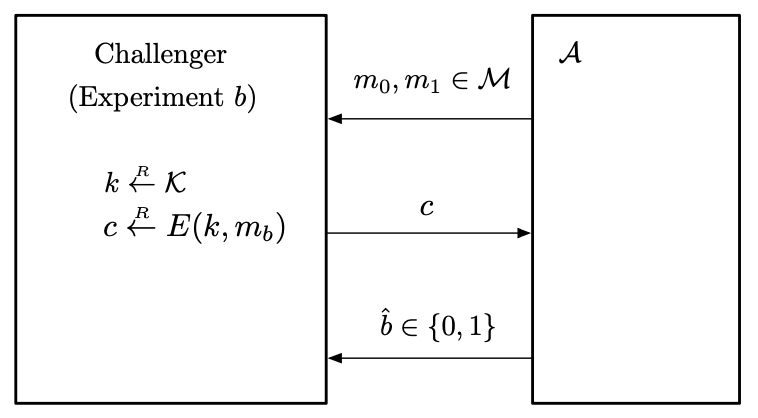
\includegraphics[width=0.5\linewidth]{figures/chapter2/fig1.png}
  \caption{攻击游戏 \ref{game:2-1} 中的实验 $b$}
  \label{fig:2-1}
\end{figure}

\begin{definition}[语义安全性]\label{def:2-2}
如果对于所有有效对手 $\mathcal{A}$,${\rm SS\mathsf{adv}}[\mathcal{A},\mathcal{E}]$ 的值都可以忽略不计,我们就称密码 $\mathcal{E}$ 是\textbf{语义安全}的。
\end{definition}

作为一个正式的定义,这还不是很完整,因为我们还没有定义``相同长度的消息"、``有效对手"和``可忽略不计"是什么意思。我们很快就会回到这个问题上。

让我们把这个正式定义与前面的讨论联系起来。假设攻击游戏 \ref{game:2-1} 中的对手 $\mathcal{A}$ 是确定性的。首先,对手以一种确定性的方式计算出消息 $m_0$和$m_1$,然后考察密文 $c$ 上的谓词 $\phi$,如果结果为真就输出 $1$,为假则输出 $0$。语义安全的意思是,式 \ref{eq:2-4} 中的 $\epsilon$ 是可以忽略不计的。如果 $\mathcal{A}$ 是概率性的,我们可以将 $\mathcal{A}$ 看作是这样的结构:它从某个适当的集合中生成一个随机数 $r$,并确定性地计算取决于$r$的消息 $m^{(r)}_0$ 和 $m^{(r)}_1$,接着评估谓词 $\phi^{(r)}$,它也取决于 $r$。这里,语义安全说明,当用 $m^{(r)}_0$、$m^{(r)}_1$ 和 $\phi^{(r)}$ 替换式 \ref{eq:2-4} 中的 $m_0$、$m_1$ 和 $\phi$ 时,$\epsilon$ 的大小仍然是可以忽略不计的,但现在的概率是针对一个随机选择的密钥和随机选择的 $r$ 值而言的。

\begin{remark}
现在让我们说一下,为什么我们要求在攻击游戏 \ref{game:2-1} 中,对手 $\mathcal{A}$ 计算出来的消息 $m_0$ 和 $m_1$ 必须是相同长度的。
\begin{itemize}
	\item 首先,消息的``长度"概念是针对特定的消息空间 $\mathcal{M}$ 而言的。换句话说,在指定一个消息空间时,我们必须指定一个规则,它能将长度(一个非负整数)与任何给定的消息关联起来。对于大多数具体的消息空间来说,这种联系是很显然的。例如,对于消息空间 $\{0, 1\}^{\leq L}$ (如例 \ref{exmp:2-2})来说,消息 $m\in\{0, 1\}^{\leq L}$ 的长度就是它的比特位数 $|m|$。然而,为了使我们的定义具有一定的普遍性,我们把长度的概念作为一个抽象概念。事实上,有些消息空间可能没有特别的长度概念,在这种情况下,所有的消息都可以被看作是长度为 $0$ 的。
	\item 其次,要求 $m_0$ 和 $m_1$ 具有相同的长度,意味着对手不会因为能够有效地根据长度区分两条密文就被认为是破坏了系统。这就是我们的正式定义所捕捉到的概念,即消息的加密被允许泄露消息的长度(但不会泄露其他信息)。
		
	我们在例 \ref{exmp:2-5} 中已经讨论过,在某些应用中,泄露消息的长度可能会带来灾难性的后果。然而,由于这个问题没有通用的解决方案,大多数现实世界的加密方案(例如TLS)根本没有尝试去隐藏消息的长度。这可能会导致真正的攻击。例如,Chen 等人表明,加密消息的长度可以揭示用户提供给云应用程序的私人数据的大量信息。他们以一个在线报税系统为例,但也有其他工作表明这种类型的攻击同样适用于很多其他的系统。
\end{itemize}
\end{remark}

\begin{example}\label{exmp:2-9}
令 $\mathcal{E}$ 是一个确定性密码,且是完美安全的。那么很容易看出,对于任意对手 $\mathcal{A}$(无论是否有效),我们都有 ${\rm SS\mathsf{adv}}[\mathcal{A},\mathcal{E}]=0$。这几乎可以立即从定理 \ref{theo:2-3} 中得出(唯一稍微复杂的是,我们在攻击游戏 \ref{game:2-1} 中的对手 $\mathcal{A}$ 可能是概率性的,但这很容易处理)。特别是,$\mathcal{E}$ 是语义安全的。因此,如果 $\mathcal{E}$ 是一次性密码本(见例 \ref{exmp:2-1}),那么对于所有对手 $\mathcal{A}$,我们有 ${\rm SS\mathsf{adv}}[\mathcal{A},\mathcal{E}]=0$,因此一次性密码本是语义安全的。由于语义安全的定义对于变长的消息空间来说是比较宽容的,所以也很容易看出,如果$\mathcal{E}$是变长一次性密码本(见例 \ref{exmp:2-2}),那么对于所有对手 $\mathcal{A}$,${\rm SS\mathsf{adv}}[\mathcal{A},\mathcal{E}]=0$都成立,因此变长一次性密码本也是语义安全的。
\end{example}

关于``有效"和``可忽略不计"这两个词,我们还要多说几句。在下面的 \ref{sec:2-3} 节中,我们将填补其余的细节(这些细节可能会稍显乏味,而且实际上并不是很有启发性)。 直观地说,\emph{可忽略不计}的意思是小到``对所有实际用途来说都是零":想像一下 $2^{-100}$ 这样的数字,如果你在下一年自燃的概率是 $2^{-100}$,那么你就不会担心这种事件的发生。我们还使用下列术语:
\begin{itemize}
	\item 一个\emph{有效对手}是一个能在``合理"时间内运行的对手。
	\item 如果 ${1}/{N}$ 可以忽略不计,就称$N$是\emph{超多项式(super-poly)}的。
	\item 一个\emph{多项式边界(poly-bounded)}的值是一个``合理"大小的数字。特别地,我们可以说,一个有效对手的运行时间是多项式边界的。
\end{itemize}

\begin{fact}\label{fact:2-6}
如果 $\epsilon$ 和 $\epsilon'$ 是两个可以忽略不计的值,而 $Q$ 和 $Q'$ 是两个多项式边界的值,那么:
\begin{enumerate}[(i)]
	\item $\epsilon+\epsilon'$ 是一个可以忽略不计的值,
	\item $Q + Q'$ 和 $Q\cdot Q'$ 都是多项式边界的,且
	\item $Q\cdot\epsilon$ 是一个可以忽略不计的值。
\end{enumerate}
\end{fact}



现在,读者可以把这些事实作为公理。我们不纠缠于这些技术问题,而是讨论一个例子,说明在分析一个使用语义安全密码的更大系统的安全性时,我们通常如何\emph{使用}这个定义。

\subsection{与较弱的安全概念的联系}\label{subsec:2-2-3}

\subsubsection{消息恢复攻击}\label{subsubsec:2-2-3-1}

直观地说,在消息恢复攻击(message recovery attack)中,对手被给定一个随机消息的加密,并且能够以明显优于随机猜测的概率(即概率为 ${1}/{|\mathcal{M}|}$)从密文中恢复消息。当然,任何合理的安全概念都应该排除这种攻击,语义安全当然也是如此。

虽然这在直觉上似乎是显而易见的,但我们给出了这一点的正式证明。我们这样做的动机之一是为了详细说明\emph{安全归约(security reduction)}的概念,这是用于推理系统安全性的主要技术。基本上,该证明将论证,任何能够有效地对 $\mathcal{E}$ 发起消息恢复攻击的有效对手 $\mathcal{A}$,都可以被用于建立一个能够破坏 $\mathcal{E}$ 的语义安全性的有效对手 $\mathcal{B}$;由于语义安全性意味着不存在这样的 $\mathcal{B}$,我们就可以得出结论,这样的 $\mathcal{A}$也是不存在的。

为了更详细地给出这个证明,我们需要一个消息恢复攻击的正式定义。和以前一样,这也是通过一个攻击游戏来完成的,该攻击游戏是一个挑战者与一个对手之间的游戏。

\begin{game}[消息恢复]\label{game:2-2}
给定一个定义在 $(\mathcal{K},\mathcal{M},\mathcal{C})$ 上的密码 $\mathcal{E}=(E,D)$,对于一个给定对手 $\mathcal{A}$,攻击游戏的过程如下:
\begin{itemize}
	\item 挑战者计算 $m\overset{\rm R}\leftarrow\mathcal{M}$,$k\overset{\rm R}\leftarrow\mathcal{K}$,$c\overset{\rm R}\leftarrow E(k,m)$,并将 $c$ 发送给对手。
	\item 对手输出一条消息 $\hat m\in\mathcal{M}$。
\end{itemize}
令 $W$ 为 $\hat m=m$ 成立的事件。我们称,在这种情况下,$\mathcal{A}$ 赢得该游戏。我们将对手 $\mathcal{A}$ 相对于 $\mathcal{E}$ 的\textbf{消息恢复优势}定义为:
$$
{\rm MR\mathsf{adv}}[\mathcal{A},\mathcal{E}]:=|\Pr[W] -{1}/{|\mathcal{M}|}|
$$
\end{game}

\begin{definition}[针对消息恢复的安全性]
如果对于所有有效对手 $\mathcal{A}$,${\rm MR\mathsf{adv}}[\mathcal{A},\mathcal{E}]$ 的值都可以忽略不计,我们就说密码 $\mathcal{E}$ \textbf{对消息恢复是安全的}。
\end{definition}

\begin{theorem}\label{theo:2-7}
令 $\mathcal{E}=(E,D)$ 是一个定义在 $(\mathcal{K},\mathcal{M},\mathcal{C})$ 上的密码。如果 $\mathcal{E}$ 是语义安全的,那么 $\mathcal{E}$ 对消息恢复也是安全的。
\end{theorem}

\begin{proof}
假设 $\mathcal{E}$ 是语义安全的。我们的目标是证明 $\mathcal{E}$ 对于消息恢复也是安全的。

为了证明 $\mathcal{E}$ 对于消息恢复是安全的,我们必须证明每一个有效对手 $\mathcal{A}$ 在攻击游戏 \ref{game:2-2} 中的优势都可忽略不计。为了证明这一点,我们给定一个任意但高效的对手 $\mathcal{A}$,现在我们的目标是证明 $\mathcal{A}$ 的消息恢复优势 ${\rm MR\mathsf{adv}}[\mathcal{A},\mathcal{E}]$ 是可以忽略不计的。令 $p$ 为 $\mathcal{A}$ 赢得消息恢复游戏的概率,那么有:
$$
{\rm MR\mathsf{adv}}[\mathcal{A},\mathcal{E}]=\left|p-{1}/{|\mathcal{M}|}\right|
$$
我们下面展示如何构建一个有效对手 $\mathcal{B}$,其在攻击游戏 \ref{game:2-1} 中的语义安全优势与 $\mathcal{A}$ 在攻击游戏 \ref{game:2-2} 中的消息恢复优势有如下关系:
\begin{equation}\label{eq:2-5}
{\rm MR\mathsf{adv}}[\mathcal{A},\mathcal{E}]\leq{\rm SS\mathsf{adv}}[\mathcal{B},\mathcal{E}]
\end{equation}
由于 $\mathcal{B}$ 是有效的,且我们假设 $\mathcal{E}$ 是语义安全的,因此式 \ref{eq:2-5} 中不等号右侧的值可以忽略不计,由此我们可以得出结论:${\rm MR\mathsf{adv}}[\mathcal{A},\mathcal{E}]$ 也可以忽略不计。

因此,完成证明所剩下的工作就是说明如何构造一个满足式 \ref{eq:2-5} 要求的有效的 $\mathcal{B}$。我们的想法是把 $\mathcal{A}$ 作为一个``黑箱",因为我们根本不需要了解 $\mathcal{A}$ 的内部运作情况。

以下是 $\mathcal{B}$ 的工作方式。对手 $\mathcal{B}$ 产生两条随机消息 $m_0,m_1\in\mathcal{M}$,并将其发送给自己的语义安全挑战者。这个挑战者向 $\mathcal{B}$ 发送一条密文 $c$,$\mathcal{B}$ 将其转发给 $\mathcal{A}$,\emph{就像它来自 $\mathcal{A}$ 的消息恢复挑战者一样}。当 $\mathcal{A}$ 输出一个信息 $\hat m$ 时,如果 $\hat m=m_1$,我们的对手 $\mathcal{B}$ 就输出 $\hat b=1$,否则输出 $\hat b=0$。

这就完成了对 $\mathcal{B}$ 的描述。注意,$\mathcal{B}$ 的运行时间与 $\mathcal{A}$ 的运行时间基本相同。我们现在分析 $\mathcal{B}$ 的语义安全优势,并将其与 $\mathcal{A}$ 的消息恢复优势关联起来。

对于 $b=0,1$,令 $p_b$ 表示当 $\mathcal{B}$ 的语义安全挑战者加密了 $m_b$ 时,$\mathcal{B}$ 的输出为 $1$ 的概率。根据定义,我们有:
$$
{\rm SS\mathsf{adv}}[\mathcal{B},\mathcal{E}]=|p_1-p_0|
$$
一方面,当 $c$ 是对 $m_1$ 的加密时,概率 $p_1$ 正好等于 $\mathcal{A}$ 在消息恢复游戏中获胜的概率,所以 $p_1=p$。另一方面,当 $c$ 是对 $m_0$ 的加密时,对手 $\mathcal{A}$ 的输出与 $m_1$ 无关,所以有$p_0={1}/{|\mathcal M|}$。由此可见:
$$
{\rm SS\mathsf{adv}}[\mathcal{B},\mathcal{E}]=|p_1-p_0|=|p-{1}/{|\mathcal{M}|}|={\rm MR\mathsf{adv}}[\mathcal{A},\mathcal{E}]
$$
这就证明了式 \ref{eq:2-5}。事实上,式 \ref{eq:2-5} 中的等号是成立的,但这对本证明并不重要。
\end{proof}

读者应该确保自己理解这个证明的逻辑,因为这种类型的证明将在本书中反复使用。我们再回顾一下该证明的重要部分,并给出另一种思考方式。

证明的核心建立在以下事实上:对于每一个在攻击游戏 \ref{game:2-2} 中攻击 $\mathcal{E}$ 的有效消息恢复对手 $\mathcal{A}$ ,都存在一个在攻击游戏 \ref{game:2-1} 中攻击 $\mathcal{E}$ 的有效语义安全对手 $\mathcal{B}$,使得:
\begin{equation}\label{eq:2-6}
{\rm MR\mathsf{adv}}[\mathcal{A},\mathcal{E}]\leq{\rm SS\mathsf{adv}}[\mathcal{B},\mathcal{E}]
\end{equation}
我们试图证明,如果 $\mathcal{E}$ 是语义安全的,那么 $\mathcal{E}$ 对消息恢复也是安全的。在上面的证明中,我们认为如果 $\mathcal{E}$ 是语义安全的,那么式 \ref{eq:2-6} 的右手边一定是可以忽略的,因此式 \ref{eq:2-6} 的右手边也一定是可以忽略的;由于这对所有有效对手 $\mathcal{A}$ 都是成立的,我们就能得出结论:$\mathcal{E}$ 对消息恢复是安全的。

证明该定理的另一种方法是反证法:如果 $\mathcal{E}$ 对消息恢复不是安全的,那么 $\mathcal{E}$ 也不是语义安全的。因此,我们假设 $\mathcal{E}$ 对消息恢复不安全。这意味着存在一个有效对手 $\mathcal{A}$,其消息恢复优势是不可忽略不计的。利用 $\mathcal{A}$,我们建立一个满足式 \ref{eq:2-6} 的有效对手 $\mathcal{B}$。根据假设,${\rm MR\mathsf{adv}}[\mathcal{A},\mathcal{E}]$ 是不可忽略不计的,而式 \ref{eq:2-6} 意味着 ${\rm SS\mathsf{adv}}[\mathcal{B},\mathcal{E}]$ 也只能是不可忽略的。由此,我们得出结论,$\mathcal{E}$ 不是语义安全的。

说得更简单些:为了证明语义安全意味着针对消息恢复的安全,我们展示了如何将一个可以打破消息恢复的有效对手转化成一个可以打破语义安全性的有效对手。

我们还强调,证明中构建的对手 $\mathcal{B}$ 只是将 $\mathcal{A}$ 作为一个``黑箱"。事实上,我们之后将要看到的几乎所有构造都是这种类型的。$\mathcal{B}$ 本质上只是 $\mathcal{A}$ 的一个包装,它由 $\mathcal{B}$ 的挑战者和 $\mathcal{A}$ 的单个运行实例之间的一些简单有效的``接口层"组成。理想情况下,我们希望接口层的计算复杂性不依赖于 $\mathcal{A}$ 的计算复杂性;然而,一些依赖性是不可避免的:如果一个攻击游戏允许 $\mathcal{A}$ 向其挑战者进行多次查询,$\mathcal{A}$ 的查询次数越多,接口层必须执行的工作就越多,但这个工作应该只依赖于查询的数量,而不是 $\mathcal{A}$ 的运行时间。

因此,当对手 $\mathcal{B}$ 可以像上述那样被结构化为与 $\mathcal{A}$ 互动的有效接口时,我们就称它是一个围绕对手 $\mathcal{A}$ 的\textbf{基本包装器(elementary wrapper)}。其突出的特性是:
\begin{itemize}
	\item 如果 $\mathcal{B}$ 是一个围绕 $\mathcal{A}$ 的基本包装器,并且 $\mathcal{A}$ 是有效的,那么 $\mathcal{B}$ 也是有效的。
	\item 如果 $\mathcal{C}$ 是一个围绕 $\mathcal{B}$ 的基本包装器,而 $\mathcal{B}$ 是 $\mathcal{A}$ 的一个基本包装器,那么 $\mathcal{C}$ 也是一个 $\mathcal{A}$ 的基本包装器。
\end{itemize}

\subsubsection{计算消息的单个比特}

如果一个加密方案是安全的,我们不仅应该很难恢复整个消息,也应该很难计算出关于消息的任何部分的信息。

我们不会在这里证明一个完全通用的定理,而是考虑一个具体的例子。

假设 $\mathcal{E}=(E,D)$ 是一个定义在 $(\mathcal{K},\mathcal{M},\mathcal{C})$ 上的密码,其中 $\mathcal{M}=\{0,1\}^L$。对于 $m\in\mathcal{M}$,如果 $m$ 中比特 $1$ 的数量是奇数,我们就定义 ${\rm parity}(m)$ 为的值 $1$,否则为 $0$。与这个结论等价的另一个结论是,${\rm parity}(m)$ 的值就等于对构成 $m$ 的所有比特做异或操作的结果。

我们将证明,如果 $\mathcal{E}$ 是语义安全的,那么给定一个随机消息 $m$ 的加密 $c$,很难预测 ${\rm parity}(m)$。由于 ${\rm parity}(m)$ 是一个 $1$ 比特的信息,任何对手都可以通过随机猜测以 ${1}/{2}$ 的概率猜中这个值。尽管如此,我们想要说明的是,没有任何有效对手能够稍微提升哪怕一点猜中的概率。

作为热身,假设有一个有效对手 $\mathcal{A}$ 能够以 $1$ 的概率猜中 ${\rm parity}(m)$。这意味着,对于每个消息 $m$,每个密钥 $k$,以及 $m$ 的每个加密 $c$,当我们向 $\mathcal{A}$ 提供密文 $c$ 时,它就能够输出 $m$ 的奇偶性。我们的对手任意选择两条消息 $m_0$ 和 $m_1$,但 ${\rm parity}(m_0)=0$,${\rm parity}(m_1)=1$。然后,它把这两条消息交给自己的语义安全挑战者,得到一个密文 $c$,然后将其转发给 $\mathcal{A}$。在收到 $c$ 后,对手 $\mathcal{A}$ 输出一个比特 $\hat b$,而 $\mathcal{B}$ 输出这个相同的比特 $\hat b$ 作为它自己的输出。很容易看出,$\mathcal{B}$ 的语义安全优势恰好是 $1$:当它的语义安全挑战者加密的是 $m_0$ 时,它总是输出 $0$,而当它的语义安全挑战者加密的是 $m_1$ 时,它总是输出 $1$。

这表明,如果 $\mathcal{E}$ 是语义安全的,就不存在能以 $1$ 的概率预测奇偶性的有效对手。然而,我们可以再进一步:如果 $\mathcal{E}$ 是语义安全的,就不存在能以明显优于 ${1}/{2}$ 的概率预测奇偶性的有效对手。为了准确说明这一点,我们给出一个攻击游戏。

\begin{game}[奇偶性预测]\label{game:2-3}
给定一个定义在 $(\mathcal{K},\mathcal{M},\mathcal{C})$ 上的密码 $\mathcal{E}=(E,D)$,对于一个给定对手 $\mathcal{A}$,攻击游戏的过程如下:
\begin{itemize}
	\item 挑战者计算 $m\overset{\rm R}\leftarrow\mathcal{M}$,$k\overset{\rm R}\leftarrow\mathcal{K}$,$c\overset{\rm R}\leftarrow E(k,m)$,并将 $c$ 发送给对手。
	\item 对手输出 $\hat b\in\{0,1\}$。
\end{itemize}

令 $W$ 为 $\hat b={\rm parity}(m)$ 的事件。我们定义 $\mathcal{A}$ 对于 $\mathcal{E}$ 的\textbf{奇偶性预测优势}为:
$$
{\rm Parity\mathsf{adv}}[\mathcal{A},\mathcal{E}]:=|\Pr[W]-{1}/{2}|
$$
\end{game}

\begin{definition}[奇偶性预测]
如果对于所有有效对手 $\mathcal{A}$,${\rm Parity\mathsf{adv}}[\mathcal{A},\mathcal{E}]$ 的值都可以忽略不计,我们就称密码 $\mathcal{E}$ \textbf{对奇偶性预测是安全的}。
\end{definition}

\begin{theorem}
令 $\mathcal{E}=(E,D)$ 是一个定义在 $(\mathcal{K},\mathcal{M},\mathcal{C})$ 上的密码,其中 $\mathcal{M}=\{0,1\}^L$。如果 $\mathcal{E}$ 是语义安全的,那么 $\mathcal{E}$ 对奇偶性预测是安全的。
\end{theorem}

\begin{proof}
与定理 \ref{theo:2-7} 的证明一样,我们也给出一个基于归约的证明。特别地,我们将证明,对于每个按照攻击游戏 \ref{game:2-3} 攻击 $\mathcal{E}$ 的奇偶性预测对手 $\mathcal{A}$,都存在一个按照攻击游戏 \ref{game:2-1} 攻击 $\mathcal{E}$ 的语义安全对手 $\mathcal{B}$,其中 $\mathcal{B}$ 是一个围绕 $\mathcal{A}$ 的基本包装器,满足:
$$
{\rm Parity\mathsf{adv}}[\mathcal{A},\mathcal{E}]=\frac{1}{2}\cdot{\rm SS\mathsf{adv}}[\mathcal{B},\mathcal{E}]
$$

令 $\mathcal{A}$ 是一个奇偶性预测对手,它能以 ${1}/{2}+\epsilon$ 的概率预测奇偶性,那么有 ${\rm Parity\mathsf{adv}}[\mathcal{A},\mathcal{E}]=\epsilon$。

下面我们展示,如何构建我们的语义安全对手 $\mathcal{B}$。

我们的对手 $\mathcal{B}$ 生成一个随机消息 $m_0$,并设置 $m_1\leftarrow m_0\oplus(0^{L-1}||1)$。也就是说,$m_1$ 除了最后一位被翻转之外,其他各位都与 $m_0$ 相同。因此 $m_0$ 与 $m_1$ 的奇偶性正好相反。

我们的对手 $\mathcal{B}$ 将这对 $m_0$,$m_1$ 发送给它自己的语义安全挑战者,并从挑战者那里收到一条密文 $c$,然后将 $c$ 转发给 $\mathcal{A}$。当 $\mathcal{A}$ 输出一个比特 $\hat b$ 时,如果 $\hat b={\rm parity}(m_0)$,我们的对手 $\mathcal{B}$ 就输出 $1$,否则就输出 $0$。

对于 $b=0,1$,令 $p_b$ 是当对手 $\mathcal{B}$ 的语义安全挑战者加密了 $m_b$ 的情况下对手 $\mathcal{B}$ 输出为 $1$ 的概率。所以根据定义,我们有:
$$
{\rm SS\mathsf{adv}}[\mathcal{B},\mathcal{E}]=|p_1-p_0|
$$

我们声称 $p_0={1}/{2}+\epsilon$,$p_1={1}/{2}-\epsilon$。这是因为,无论是加密的是 $m_0$ 还是 $m_1$,$m_b$ 在 $\mathcal{M}$ 上的分布都是均匀的,因此在 $b=0$ 的情况下,我们的奇偶性预测者 $\mathcal{A}$ 将以 ${1}/{2}+\epsilon$ 的概率输出 ${\rm parity}(m_0)$;而当 $b=1$ 时,我们的奇偶性预测者 $\mathcal{A}$ 将以 ${1}/{2}+\epsilon$ 的概率输出 ${\rm parity}(m_1)$,也就是以 $1-({1}/{2}+\epsilon)={1}/{2}-\epsilon$ 的概率输出 ${\rm parity}(m_0)$。

因此:
$$
{\rm SS\mathsf{adv}}[\mathcal{B},\mathcal{E}]=|p_1-p_0|=2|\epsilon|=2\cdot{\rm Parity\mathsf{adv}}[\mathcal{A},\mathcal{E}]
$$
这就证明了该定理。
\end{proof}

我们已经表明,如果一个对手能够有效地预测一条消息的奇偶性,那么它就可以被用来破坏语义安全。反过来说,事实证明,如果一个对手能够破坏语义安全,它就能有效地预测消息的某些谓词(见练习 3.15)。

\subsection{语义安全的结果}\label{subsec:2-2-4}

在本节中,我们将在一个具体的例子,即电子赌博的背景下研究语义安全的后果。这个例子的具体细节并不那么重要,但是这个例子说明了人们通常是如何在应用中使用语义安全假设的。

考虑下面这个极其简化的轮盘赌版本,它是一种在\emph{庄荷(house)}与一个\emph{玩家(player)}之间进行的游戏。玩家给庄荷 1 美元,然后它可以下两种赌注中的一种:
\begin{itemize}
	\item ``高或低",或者
	\item ``偶或奇"。
\end{itemize}
下注后,庄荷随机选择一个数字 $r\in\{0,1,...,36\}$。当 $r\neq 0$,并且:
\begin{itemize}
	\item 玩家下注``高",且 $r>18$,
	\item 玩家下注``低",且 $r\leq18$,
	\item 玩家下注``偶",且 $r$ 为偶数,
	\item 玩家下注``奇",且 $r$ 为奇数。
\end{itemize}
时,玩家获胜。如果玩家赢了,庄荷将付给它 2 美元(即玩家净赚 1 美元);如果玩家输了,庄荷将不会付给它钱(即玩家净输 1 美元)。显然,在这个游戏中,庄荷有一个虽然小但仍然显著的优势:玩家获胜的概率是 $18/37\approx48.65\%$。

现在,假设这个游戏是在互联网上进行的。此外,假设由于各种技术原因,在玩家下注\emph{之前},赌场需要公布 $r$ 的加密(也许是由一些与赌场共享密钥的监管机构来解密)。玩家可以在下注前自由地分析这个加密消息,以此试图来增加它赢钱的机会。然而,如果这个密码是好的,玩家的机会应该不能增加很多。让我们来证明这一点,假设 $r$ 是用定义在 $(\mathcal{K},\mathcal{M},\mathcal{C})$ 上的一个密码 $\mathcal{E}=(E,D)$ 加密的,其中 $\mathcal{M}=\{0,1,...,36\}$(在这个例子中,我们将 $\mathcal{M}$ 中的所有消息视为具有相同的长度)。另外,从现在开始,让我们称玩家为 $\mathcal{A}$,以强调玩家的对抗性,并假设 $\mathcal{A}$ 的策略可以被建模为一种有效算法。图 \ref{fig:2-2} 展示了这个游戏。这里,\emph{赌注(bet)}表示``高"、``低"、``偶"、``奇"中的一个。玩家 $\mathcal{A}$ 将赌注发送给庄荷,庄荷会评估函数 $W(r,bet)$。如果赌注相对于$r$而言是获胜的,函数的值就为$1$,否则就为$0$。我们定义:
$$
{\rm IR\mathsf{adv}}[A]:=|\Pr[W (r,bet)=1]-{18}/{37}|
$$

我们的目标是要证明以下定理。

\begin{figure}
  \centering
  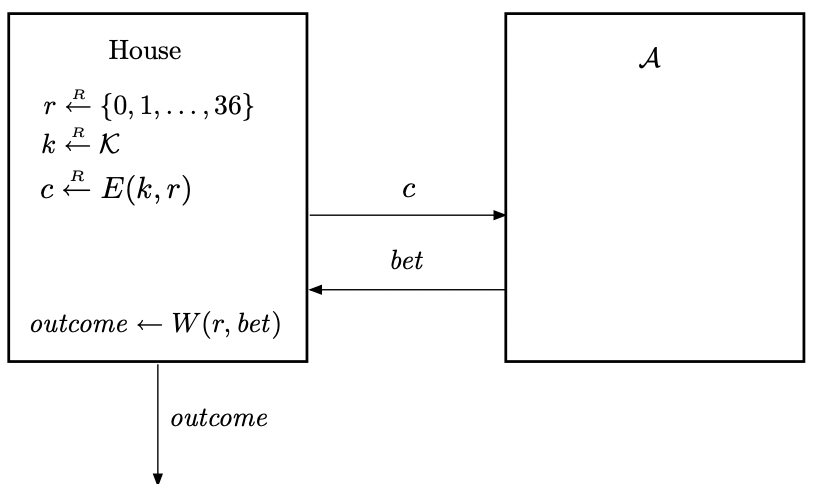
\includegraphics[width=0.6\linewidth]{figures/chapter2/fig2.png}
  \caption{网络轮盘赌}
  \label{fig:2-2}
\end{figure}

\begin{theorem}
如果 $\mathcal{E}$ 是语义安全的,那么对于每个有效玩家 $\mathcal{A}$,${\rm IR\mathsf{adv}}[\mathcal{A}]$ 的值都可忽略不计。
\end{theorem}

\begin{proof}
如我们在 \ref{subsec:2-2-3} 节所做的那样,我们仍然通过安全归约来证明这一点。更具体地说,我们将证明,对于每个玩家 $\mathcal{A}$,都存在一个语义安全对手 $\mathcal{B}$,使得 $\mathcal{B}$ 是 $\mathcal{A}$ 的一个基本包装器,并且:
\begin{equation}\label{eq:2-7}
{\rm IR\mathsf{adv}}[A]={\rm SS\mathsf{adv}}[\mathcal{B},\mathcal{E}]
\end{equation}

因此,如果存在一个优势不可忽略不计的有效玩家 $\mathcal{A}$,我们就能够得到一个有效的语义安全对手 $\mathcal{B}$,它可以打破 $\mathcal{E}$ 的语义安全性,而我们已经假设这是不可能的。因此,不存在这样的 $\mathcal{A}$。

为了分析我们的新对手 $\mathcal{B}$,我们先考虑一个``理想化"的互联网轮盘赌版本。在这个版本中,庄荷不公布实际的 $r$ 的加密,而是公布一个``假"值的加密,例如 $0$。图 \ref{fig:2-3} 展示了这个理想化的网络轮盘赌的逻辑。然而,请注意,在理想化版本的互联网轮盘赌中,庄荷仍然使用 $r$ 的实际值来决定游戏的结果。令 $p_0$ 为 $\mathcal{A}$ 在互联网轮盘赌中获胜的概率,$p_1$ 为 $\mathcal{A}$ 在理想化互联网轮盘赌中获胜的概率。

\begin{figure}
  \centering
  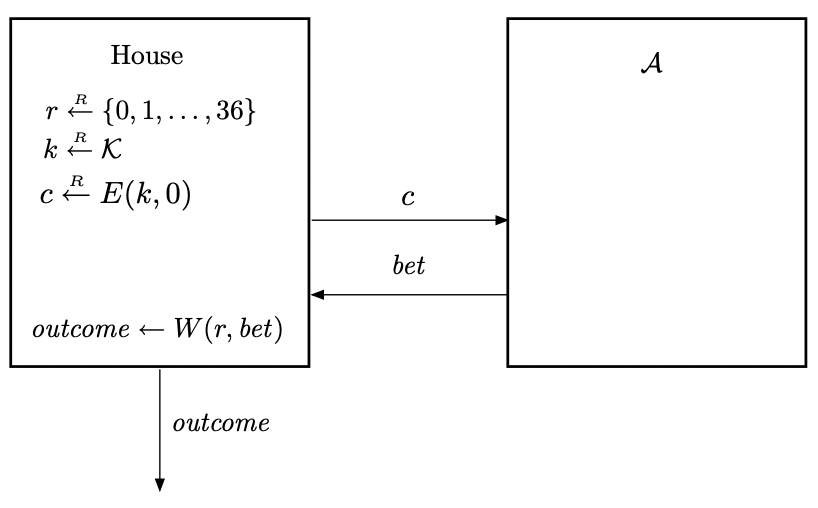
\includegraphics[width=0.6\linewidth]{figures/chapter2/fig3.png}
  \caption{网络轮盘赌的理想化版本}
  \label{fig:2-3}
\end{figure}

\begin{figure}
  \centering
  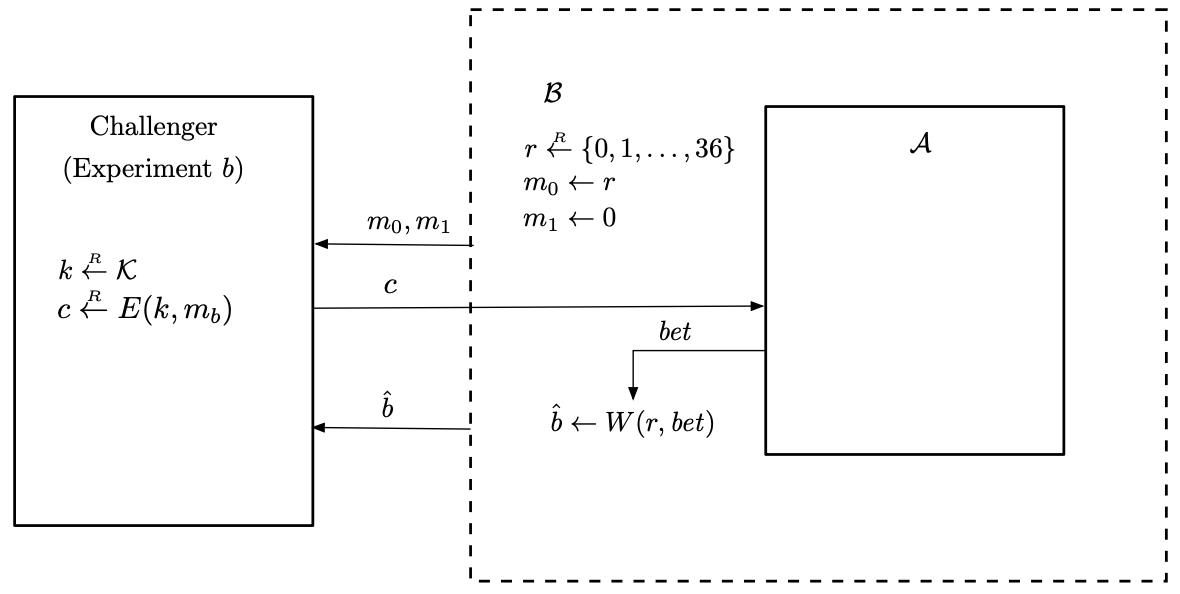
\includegraphics[width=0.85\linewidth]{figures/chapter2/fig4.png}
  \caption{攻击游戏 \ref{game:2-1} 中的语义安全对手 $\mathcal{B}$}
  \label{fig:2-4}
\end{figure}

我们的对手 $\mathcal{B}$ 被设计为在攻击游戏 \ref{game:2-1} 中进行游戏。因此,如果令 $\hat b$ 表示 $\mathcal{B}$ 在该游戏中的输出,我们有:
\begin{itemize}
	\item 如果 $\mathcal{B}$ 被置于实验 $0$ 中,那么有 $\Pr[\hat b=1]=p_0$;
	\item 如果 $\mathcal{B}$ 被置于实验 $1$ 中,那么有 $\Pr[\hat b=1]=p_1$。
\end{itemize}
图 \ref{fig:2-4} 展示了对手 $\mathcal{B}$ 的运行逻辑。通过构造可以看出,$\mathcal{B}$ 满足上面所声称的属性,特别是:
\begin{equation}\label{eq:2-8}
{\rm SS\mathsf{adv}}[\mathcal{B},\mathcal{E}]=|p_1-p_0|
\end{equation}

现在,考虑 $\mathcal{A}$ 在理想化互联网轮盘赌中获胜的概率 $p_1$。不管 $\mathcal{A}$ 的策略有多高明,它获胜的概率始终是 $18/37$,因为在这个理想化互联网轮盘赌中,\emph{赌注}的值是由 $c$ 计算出来的,而 $c$ 在统计上与 $r$ 的值毫无关系。因此:
\begin{equation}\label{eq:2-9}
{\rm IR\mathsf{adv}}[A]=|p_1-p_0|
\end{equation}

结合式 \ref{eq:2-8} 和式 \ref{eq:2-9},我们就能得到式 \ref{eq:2-7}。
\end{proof}

我们之后会反复使用这里用来分析互联网轮盘赌的方法。其基本思想是用一个理想化的系统组件替换原来的组件,然后分析这个新的、理想化版本的系统行为。

从上述例子中得到的另一个教训是,在推理一个系统的安全性时,我们将什么视为``对手",取决于我们想要做什么。在上面的分析中,我们用几个组件拼凑了一个新的对手 $\mathcal{B}$:其中一个组件是原来的对手 $\mathcal{A}$,而其他组件则是从系统的其他部分(在这个例子中是``庄荷"的算法)搜刮来的。这在我们全书的安全分析中会非常典型。直观地说,如果我们想象一个系统图,在安全分析的不同点上,我们将在系统的不同组件周围画一个圆圈,以确定我们在分析那个点时的``对手"。

\subsection{比特猜测:语义安全性的另一种表征}\label{subsec:2-2-5}

\ref{subsec:2-2-4} 小节中的例子很典型,它说明人们可以使用语义安全的定义来分析使用语义安全密码的较大系统的安全属性。然而,语义安全还有另一种更便于使用的表征,当我们试图证明一个给定的密码满足该定义时,它往往更方便使用。在这个替代性的表述中,我们定义一个新的攻击游戏。对手所扮演的角色与之前完全相同。然而,我们现在不再进行两个不同的实验,而是只有一个单一的实验。在这个\textbf{比特猜测版本(bit-guessing version)}的攻击游戏中,挑战者随机选择一个比特 $b\in\{0,1\}$并运行攻击游戏 \ref{game:2-1} 中的实验 $b$;对手的目标是以明显优于 ${1}/{2}$ 的概率猜中比特 $b$。下面是该攻击游戏的详细情况。

\begin{game}[语义安全性:比特猜测版本]\label{game:2-4}
给定一个定义在 $(\mathcal{K},\mathcal{M},\mathcal{C})$ 上的密码 $\mathcal{E}=(E,D)$,对于一个给定对手 $\mathcal{A}$,攻击游戏按如下方式运行:
\begin{itemize}
	\item 对手 $\mathcal{A}$ 计算相同长度的 $m_0, m_1\in\mathcal{M}$,并将它们发送给挑战者。
	\item 挑战者计算 $b\overset{\rm R}\leftarrow\{0,1\}$,$k\overset{\rm R}\leftarrow\mathcal{K}$,$c\overset{\rm R}\leftarrow E(k,m_b)$,并将 $c$ 发送给对手。
	\item 对手输出一个比特 $\hat b\in\{0,1\}$。
\end{itemize}

如果 $\hat b=b$,我们就称 $\mathcal{A}$ \textbf{赢得}这个游戏。
\end{game}

\begin{figure}
  \centering
  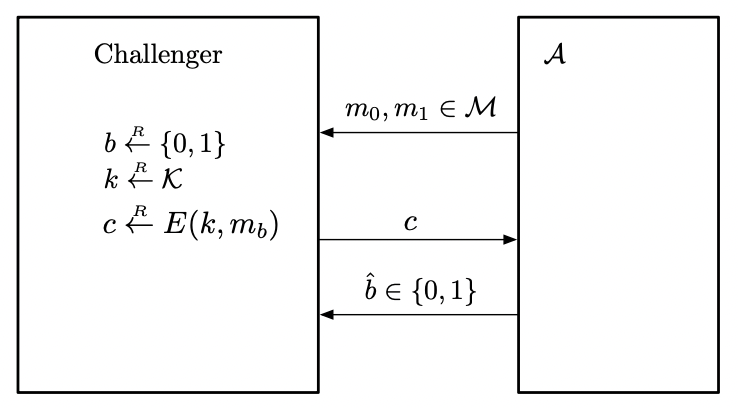
\includegraphics[width=0.5\linewidth]{figures/chapter2/fig5.png}
  \caption{攻击游戏 \ref{game:2-4}}
  \label{fig:2-5}
\end{figure}

图 \ref{fig:2-5} 展示了攻击游戏 \ref{game:2-4}。请注意,在这个游戏中,$\mathcal{A}$ 赢得游戏的事件是由 $b$ 与 $k$ 的随机选择、加密算法的随机选择(如果有的话)和对手的随机选择(如果有的话)共同构成的概率空间所定义的。

当然,任何对手都能以 ${1}/{2}$ 的概率赢得游戏,只需要完全忽略 $c$ 并随机选择 $\hat b$(或者说总是选择$\hat b=0$或总是选择$\hat b =1$)。我们感兴趣的是,对手能比随机猜测好多少。如果用 $W$ 表示对手赢得上述攻击游戏的比特猜测版本的事件,那么我们感兴趣的是 $|\Pr[W]-{1}/{2}|$ 的值,我们用 ${\rm SS\mathsf{adv}}^∗[\mathcal{A},\mathcal{E}]$ 表示该值。于是,我们有:

\begin{theorem}\label{theo:2-10}
对于每个密码 $\mathcal{E}$ 和每个对手 $\mathcal{A}$,我们都有:
\begin{equation}\label{eq:2-10}
{\rm SS\mathsf{adv}}[\mathcal{B},\mathcal{E}]= 2\cdot{\rm SS\mathsf{adv}}^∗[\mathcal{A},\mathcal{E}]
\end{equation}
\end{theorem}

\begin{proof}
这只是一个简单的计算。令 $p_0$ 是对手在攻击游戏 \ref{game:2-1} 的实验 $0$ 中输出 $1$ 的概率,$p_1$ 是对手在攻击游戏 \ref{game:2-1} 的实验 $1$ 中输出 $1$ 的概率。

现在考虑攻击游戏 \ref{game:2-4}。从现在开始,所有的事件和概率都是关于这个游戏的。如果我们以 $b=0$ 这一事件为条件,那么在这个条件概率空间中,挑战者和对手的所有其他随机选择的分布方式与攻击游戏 \ref{game:2-1} 的实验 $0$ 中的相应数值应该完全相同。因此,如果 $\hat b$ 是攻击游戏 \ref{game:2-4} 中对手的输出,则有:
$$
\Pr[\hat b=1\,|\,b=0]=p_0
$$
通过一个类似的论证,我们还可以得到:
$$
\Pr[\hat b=1\,|\,b=1]=p_1
$$
因此,我们有:
$$
\begin{aligned}
\Pr[\hat b=b]
&=\Pr[\hat b=b\,|\,b=0]\cdot\Pr[b=0]+\Pr[\hat b=b\,|\,b=1]\cdot\Pr[b=1]\\
&=\Pr[\hat b=0\,|\,b=0]\cdot \frac{1}{2}+\Pr[\hat b=b\,|\,b=1]\cdot\frac{1}{2}\\
& =\frac{1}{2}(1-\Pr[\hat b=1\,|\,b=0]+\Pr[\hat b=1\,|\,b=1])\\
& =\frac{1}{2}(1-p_0+p_1)
\end{aligned}
$$
因此:
$$
{\rm SS\mathsf{adv}}^∗[\mathcal{A},\mathcal{E}]=|\Pr[\hat b=b]-\frac{1}{2}|=\frac{1}{2}|p_1-p_0|=\frac{1}{2}\cdot{\rm SS\mathsf{adv}}[\mathcal{B},\mathcal{E}]
$$
这就证明了该定理。
\end{proof}

就像把 ${\rm SS\mathsf{adv}}[\mathcal{A},\mathcal{E}]$ 称为 $\mathcal{A}$ 的``语义安全优势"一样,我们将把 ${\rm SS\mathsf{adv}}^∗[\mathcal{A},\mathcal{E}]$ 称为 $\mathcal{A}$ 的``比特猜测语义安全优势"。

\subsubsection{一种推广}

事实证明,上面的情况是相当普遍的。虽然我们在本章中不需要它,但为了将来参考,我们在此指出如何推广上述情况到更一般的场景。我们可能会遇到一些情况,对于一些密码学系统(称为``$\mathcal{S}$"),其中的一些特定的安全属性(称为``$X$")可以用涉及两个实验(实验$0$和实验$1$)的攻击游戏来定义,其中对手 $\mathcal{A}$ 的协议在两个实验中是相同的,而挑战者的协议则是不同的。对于 $b=0,1$,我们定义 $W_b$ 为 $\mathcal{A}$ 在实验 $b$ 中输出为 $1$ 的事件,我们还定义:
$$
{\rm X\mathsf{adv}}[\mathcal{A},\mathcal{S}]:=|\Pr[W_0] -\Pr[W_1]|
$$
是 $\mathcal{A}$ 的 ``$X$ 优势"。就像上面一样,我们总是可以定义该攻击游戏的比特猜测版本,此时,挑战者随机选择一个 $b\in\{0,1\}$,然后运行实验 $b$ 作为它的协议。如果令 $W$ 是对手 $\mathcal{A}$ 的输出为 $b$ 的事件,那么我们定义:
$$
{\rm X\mathsf{adv}}^*[\mathcal{A},\mathcal{S}]:=|\Pr[W]-{1}/{2}|
$$
是 $\mathcal{A}$ 的``比特猜测$X$优势"。

使用与定理 \ref{theo:2-10} 的证明完全相同的计算方法,我们有:
\begin{equation}\label{eq:2-11}
{\rm X\mathsf{adv}}[\mathcal{A},\mathcal{S}]=2\cdot{\rm X\mathsf{adv}}^*[\mathcal{A},\mathcal{S}]
\end{equation}
\section{数学细节}\label{sec:2-3}

迄今为止,我们一直比较随意地使用\emph{有效(efficient)}和\emph{可忽略不计(negligible)}这两个术语,但没有给出它们的正式定义:
\begin{itemize}
	\item 我们要求,一个计算性密码要有\emph{有效}的加密和解密算法;
	\item 对于一个语义安全的密码,我们要求任何\emph{有效}对手在攻击游戏 \ref{game:2-1} 中的优势都\emph{可忽略不计}。
\end{itemize}
本节的目标是为这些术语提供精确的数学定义。虽然这些定义将密码学构建在坚实的数学理论基础上,并为我们的研究提供了一个令人满意的理论框架,我们仍需警告读者:
\begin{itemize}
	\item 这些定义相当复杂,需要大量的符号;并且
	\item 这些定义只是非常粗略地模拟了我们对这些术语的直观理解。
\end{itemize}
我们强调,读者可以安全地跳过这一节,而不会在理解上蒙受重大损失。在进入正式定义之前,我们先简要地告诉读者我们到底想要在这些定义中抓住哪些关键点:
\begin{itemize}
	\item 首先,当我们谈及一个有效的加密或解密算法时,我们通常指的是一种运行速度非常快的算法,比如说,以 $10$ 到 $100$ 个时钟周期每字节的速度加密数据。
	\item 其次,当我们谈及一个有效对手时,我们通常指的是一个能在某个大的,但仍然可行的时间(和其他计算资源)下完成运行的算法。通常情况下,我们假设一个试图破解密码学系统的对手愿意花费比密码学系统的使用者更多的资源。因此,$10,000$ 台计算机并行运行 $10$ 年,可以被视为一个有决心和耐心,且财力雄厚的对手的可行计算上限。然而,在某些情况下,比如在 \ref{subsec:2-2-4} 小节的网络轮盘赌的例子中,对手的计算时间可能会受到更大的限制。
	\item 第三,当我们说对手的优势可忽略不计时,我们的意思是,该优势是如此之小,以至于就所有实际目的而言,它都可以被视为等于零。正如我们在网络轮盘赌的例子中所看到的,如果在攻击游戏 \ref{game:2-1} 中,没有一个有效对手拥有超过 $2^{-100}$ 的优势,那么在实践中,也就没有一个玩家可以将它在网络轮盘赌中获胜的概率提升到 $2^{-100}$ 以上。
\end{itemize}

尽管我们对\emph{有效}一词的直观理解取决于上下文,但我们的正式定义不会做任何这种类型的区分。事实上,我们将采用计算复杂性理论的习惯,把\emph{有效}算法的概念等同于\emph{(概率性)多项式时间}算法的概念。无论好坏,这都为我们提供了一个独立于任何特定计算模型具体细节的形式化框架。

\subsection{可忽略不计、超多项式与多项式边界函数}\label{subsec:2-3-1}

我们首先从对\emph{可忽略不计(negligible)}、\emph{超多项式(super-poly)}和\emph{多项式边界(poly-bounded)}函数这三个概念的定义开始。

直观地讲,一个可忽略不计函数 $f:\mathbb{Z}_{\geq0}\to\mathbb{R}$ 是一个不仅在 $n\to\infty$ 时趋近于 $0$,而且趋近于 $0$ 的速度比任何多项式的倒数都要更快的函数。

\begin{definition}\label{def:2-5}
如果对于所有的 $c\in\mathbb{R}_{>0}$,都存在 $n_0\in\mathbb{Z}_{\geq 1}$ 使得对于所有的整数 $n\geq n_0$,都有 $|f(n)|<{1}/{n^c}$ 成立,我们就称函数 $f:\mathbb{Z}_{\geq1}\to\mathbb{R}$ 是\textbf{可忽略不计的(negligible)}。
\end{definition}

可忽略不计函数还有一种更加便于理解和使用的表示,如下所示:

\begin{theorem}\label{theo:2-11}
当且仅当对于所有的 $c>0$,都有:
\[
\lim_{n\to\infty}f(n)n^c=0
\]
时,函数 $f:\mathbb{Z}_{\geq1}\to\mathbb{R}$ 是可忽略不计的。
\end{theorem}

\begin{proof}
留作练习。
\end{proof}

\begin{example}\label{exmp:2-10}
一些不可忽略不计函数实例:
\[
2^{-n},
\quad
2^{-\sqrt{n}},
\quad
n^{-\log n}
\]
一些可忽略不计函数实例:
\[
\frac{1}{1000n^4+n^2\log n},
\quad
\frac{1}{n^{100}}
\]
\end{example}

当我们正式定义了``可忽略不计"这个术语后,定义``超多项式"就很容易了:

\begin{definition}\label{def:2-6}
如果 $1/f$ 可忽略不计,我们就称函数 $f:\mathbb{Z}_{\geq1}\to\mathbb{R}$ 是\textbf{超多项式的(super-poly)}。
\end{definition}

本质上,一个多项式边界函数 $f:\mathbb{Z}_{\geq1}\to\mathbb{R}$ 是一个被某个多项式(的绝对值)约束的函数。严格地说:

\begin{definition}\label{def:2-7}
如果存在 $c,d\in\mathbb{R}_{>0}$ 使得对于所有的整数 $n\geq0$,都有 $|f(n)|\leq n^c+d$,我们就称函数 $f:\mathbb{Z}_{\geq1}\to\mathbb{R}$ 是\textbf{多项式边界的(poly-bounded)}。
\end{definition}

请注意,如果 $f$ 是一个多项式边界函数,$1/f$ 就必然\emph{不是}一个可忽略不计函数。然而,正如下面的例子所说明的那样,请务必注意不要得出错误的推论。

\begin{example}\label{exmp:2-11}
定义 $f:\mathbb{Z}_{\geq1}\to\mathbb{R}$,使得对于所有偶数 $n$,都有 $f(n)={1}/{n}$;对于所有奇数 $n$,都有 $f(n)=2^{-n}$。那么 $f$ 不可忽略不计,但 $1/f$ 既不是多项式边界的,也不是超多项式的。
\end{example}

\subsection{计算性密码:正式定义}\label{subsec:2-3-2}

现在,我们讨论形式化的定义。首先,我们承认,我们之前说了个谎:当我们说一个计算性密码 $\mathcal{E}=(E,D)$ 定义在 $(\mathcal{K},\mathcal{M},\mathcal{C})$ 上,其中 $\mathcal{K}$ 是密钥空间,$\mathcal{M}$ 是消息空间,$\mathcal{C}$ 是密文空间,而且上述每个空间都是有限集时,我们并没有完全说出事实。在数学模型中(尽管在现实世界的系统中并不总是如此),我们将一个密码\emph{族} $\mathcal{E}$ 的密钥、消息和密文空间相关联,其索引为:
\begin{itemize}
	\item 一个\textbf{安全参数(security parameter)},它是一个正整数,用 $\lambda$ 表示,以及
	\item 一个\textbf{系统参数(system parameter)},它是一个比特序列,用 $\Lambda$ 表示。
\end{itemize}
因此,现在 $\mathcal{K},\mathcal{M},\mathcal{C}$ 不再单是三个有限集,而是三个有限集族:
\[
\{\mathcal{K}_{\lambda,\Lambda}\}_{\lambda,\Lambda},\quad
\{\mathcal{M}_{\lambda,\Lambda}\}_{\lambda,\Lambda},\quad
\{\mathcal{C}_{\lambda,\Lambda}\}_{\lambda,\Lambda}
\]
在本定义中,我们将其视为比特序列的集合(可以通过某些规范的编码函数来表示特定的数学对象)。

我们的想法是,当部署密码 $\mathcal{E}$ 时,安全参数 $\lambda$ 会被固定为某个值。一般来说,更大的 $\lambda$ 值往往意味着更高的安全水平(即针对拥有更多计算资源的对手的抵抗力),但这往往也意味着更长的密钥,以及更慢的加解密速度。因此,安全参数就像一个我们可以转动的``拨盘",用于在安全和效率之间设定一个权衡。

一旦选定了 $\lambda$,系统参数 $\Lambda$ 就会由一种特定于该密码的算法生成。我们的想法是,系统参数 $\Lambda$(连同 $\lambda$)给出了一种对密码的一个特定实例的详细描述,即:
\[
(\mathcal{K},\mathcal{M},\mathcal{C})
=(
\mathcal{K}_{\lambda,\Lambda},\;
\mathcal{M}_{\lambda,\Lambda},\;
\mathcal{C}_{\lambda,\Lambda}
)
\]
这一固定实例可能会被部署到一个更大的系统中,并被多方使用——$\lambda$ 和 $\Lambda$ 值都是公开的,(包括对手在内的)每个人都能知道。

\begin{example}\label{exmp:2-12}
考虑例 \ref{exmp:2-4} 中讨论的加性一次性密码本。该密码的描述中涉及到一个模数 $n$。要部署这样一个密码,需要生成一个合适的模数 $n$,并将其公开(有时甚至会将其直接``硬编码"到实现密码的程序里)。模数 $n$ 就是这个密码的系统参数。安全参数的特定值决定了 $n$ 的长度,以比特为单位。$n$ 本身可能由某些算法产生,这些算法可能是概率性的,其输出分布可能取决于预期的应用。例如,在某些场景下,我们可能希望 $n$ 是一个素数。
\end{example}

在进一步讨论之前,我们需要先定义有效算法的概念。在这个定义中,我们将只考虑以安全参数 $\lambda$ 和总长度由 $\lambda$ 的某个固定多项式约束的其他参数作为输入的算法 $A$。基本上,我们想称 $A$ 的运行时间以 $\lambda$ 的一个多项式为界,但如果 $A$ 是概率性的,情况将更加复杂:

\begin{definition}[有效算法]\label{def:2-8}
令 $A$ 是一个算法(可能是概率性的),它以一个安全参数 $\lambda\in\mathbb{Z}_{\geq1}$,以及其他被编码成的一个比特序列 $x\in\{0,1\}^{\leq p(\lambda)}$ 的若干参数作为输入,其中 $p$ 是某个固定的多项式。如果存在一个多项式边界函数 $t$ 和一个可忽略不计函数 $\epsilon$,使得对于所有的 $\lambda\in\mathbb{Z}_{\geq1}$ 和所有的 $x\in\{0,1\}^{\leq p(\lambda)}$,算法 $A$ 在输入 $(\lambda,x)$ 上的运行时间超过 $t(\lambda)$ 的概率最多为 $\epsilon(\lambda)$,我们就称 $A$ 为一个\textbf{有效算法(efficient algorithm)}。
\end{definition}

我们强调,上述定义中的概率是针对$A$的抛硬币而言的:对概率的这个约束必须对所有可能的输入$x$都成立。
\footnote{
\label{foot:2-1}
我们不坚持概率性算法在指定的时间范围内以$1$的概率停止,这样能给我们一点``回旋的余地",使得我们能够轻松地执行某些类型的随机抽样程序,这些程序没有\emph{先验的}运行时间限制,但不太可能运行非常长的时间(例如扔硬币直到出现正面)。另一种方法是约束\emph{预期的}运行时间,但由于技术原因,这被证明是有问题的。

请注意,这个有效算法的定义并不要求该算法在所有输入上都以$1$的概率停止。一个以$2^{-\lambda}$的概率进入无限循环的算法也可以满足这个定义,即使它不是以$1$的概率停止。这些问题是相当传统的。一般来说,我们只考虑在所有输入上都能以 $1$ 的概率停止的算法:这可以更自然地被看作是对算法的输出分布的要求,而不是对其运行时间的要求。
}

\vspace{5pt}

下面是一个正式定义,它抓住了由安全参数和系统参数进行参数化的系统的基本要求,并引入了更多的术语。在下面的定义中,我们用 ${\rm Supp}(P(\lambda))$ 来指代分布 $P(\lambda)$ 的\textbf{支持(support)},即算法 $P$ 在输入 $\lambda$ 上的所有可能输出的集合。

\begin{definition}\label{def:2-9}
一个\textbf{系统参数化(system parameterization)}是一个有效概率性算法 $P$,它以一个给定的安全参数 $\lambda\in\mathbb{Z}_{\geq1}$ 为输入,输出一个比特序列 $\Lambda$,称为\textbf{系统参数},其长度总是以 $\lambda$ 的一个多项式为界。我们还定义以下术语:
\begin{itemize}
	\item 对于一个由比特序列的有限集 $\mathbf{S}=\{\mathcal{S}_{\lambda,\Lambda}\}_{\lambda,\Lambda}$ 组成的集合,其中 $\lambda$ 在 $\mathbb{Z}_{\geq1}$ 上运行,$\Lambda$ 在 ${\rm Supp}(P(\lambda))$ 上运行,如果每个集合 $\mathcal{S}_{\lambda,\Lambda}$ 中所有比特序列的长度都以 $\lambda$ 的某个多项式 $p$ 为界,我们就称 $\mathbf{S}$ 为\textbf{具有系统参数化 $P$ 的空间族 (family of spaces with system parameterization $P$)}。
	\item 如果存在一个有效确定性算法,当输入 $\lambda\in\mathbb{Z}_{\geq1}$,$\Lambda\in{\rm Supp}(P(\lambda))$ 和 $s\in\{0,1\}^{\leq p(\lambda)}$ 时,能够确定 $s\in\mathcal{S}_{\lambda,\Lambda}$ 是否成立,我们就称 $\mathbf{S}$ 是\textbf{可有效识别的(efficiently recognizable)}。
	\item 如果存在一个有效概率性算法,当输入 $\lambda\in\mathbb{Z}_{\geq1}$ 和 $\Lambda\in{\rm Supp}(P(\lambda))$ 时,能够输出一个均匀分布在 $\mathcal{S}_{\lambda,\Lambda}$ 上的元素,我们就称 $\mathbf{S}$ 是\textbf{可有效采样的(efficiently sampleable)}。
	\item 如果存在一个有效确定性算法,当输入 $\lambda\in\mathbb{Z}_{\geq1}$,$\Lambda\in{\rm Supp}(P(\lambda))$ 和 $s\in\mathcal{S}_{\lambda,\Lambda}$ 时,能够输出一个非负整数,称为 $s$ 的\textbf{长度},我们就称 $\mathbf{S}$ \textbf{有一个有效长度函数(has an effective length function)}。
\end{itemize}
\end{definition}
现在,我们就可以为计算性密码给出一个完整、正式的定义:

\begin{definition}[计算性密码]\label{def:2-10}
一个\textbf{计算性密码}由一对算法 $E$ 和 $D$,以及三个具有系统参数化 $P$ 的空间族:
\[
\mathbf{K}=\{\mathcal{K}_{\lambda,\Lambda}\}_{\lambda,\Lambda},\quad
\mathbf{M}=\{\mathcal{M}_{\lambda,\Lambda}\}_{\lambda,\Lambda},\quad
\mathbf{C}=\{\mathcal{C}_{\lambda,\Lambda}\}_{\lambda,\Lambda}
\]
组成,满足:
\begin{enumerate}
	\item $\mathbf{K}$,$\mathbf{M}$和$\mathbf{C}$都是可有效识别的。
	\item $\mathbf{K}$是可有效采样的。
	\item $\mathbf{M}$有一个有效长度函数。
	\item 算法 $E$ 是一个有效概率性算法,它接受 $\lambda,\Lambda,k,m$ 作为输入,其中 $\lambda\in\mathbb{Z}_{\geq1}$,$\Lambda\in{\rm Supp}(P(\lambda))$,$k\in\mathcal{K}_{\lambda,\Lambda}$,$m\in\mathcal{M}_{\lambda,\Lambda}$,总是输出一个 $\mathcal{C}_{\lambda,\Lambda}$ 中的元素。
	\item 算法 $D$ 是一个有效确定性算法,它接受 $\lambda,\Lambda,k,c$ 作为输入,其中 $\lambda\in\mathbb{Z}_{\geq1}$,$\Lambda\in{\rm Supp}(P(\lambda))$,$k\in\mathcal{K}_{\lambda,\Lambda}$,$c\in\mathcal{C}_{\lambda,\Lambda}$,输出一个 $\mathcal{M}_{\lambda,\Lambda}$ 中的元素或一个特殊符号 $\mathsf{reject}\notin\mathcal{M}_{\lambda,\Lambda}$。
	\item 对于所有满足 $\lambda\in\mathbb{Z}_{\geq1}$,$\Lambda\in{\rm Supp}(P(\lambda))$,$k\in\mathcal{K}_{\lambda,\Lambda}$,$m\in\mathcal{M}_{\lambda,\Lambda}$ 和 $c\in{\rm Supp}(E(\lambda,\Lambda;k,m))$ 的 $\lambda,\Lambda,k,m,c$,我们都有 $D(\lambda,\Lambda;k,c)=m$。
\end{enumerate}
\end{definition}


注意,在上述定义中,加密和解密算法都接受 $\lambda$ 和 $\Lambda$ 作为辅助输入。为了与 \ref{subsec:2-2-1} 小节中所介绍的符号保持某种程度的一致性,我们将它们写成 $E(\lambda,\Lambda;\cdots)$ 和 $D(\lambda,\Lambda;\cdots)$。

\begin{example}\label{exmp:2-13}
考虑加性一次性密码本(见例 \ref{exmp:2-12})。在我们的正式框架中,安全参数 $\lambda$ 决定了模数 $n$ 的比特长度 $L(\lambda)$,也就是系统参数。系统参数生成算法将 $\lambda$ 作为输入,生成一个长度为 $L(\lambda)$ 的模数 $n$。函数 $L(\cdot)$ 应当是一个多项式边界函数。有了这个假设,很明显,系统参数生成算法满足我们对它的要求。对密钥、消息和密文空间的要求也得到了满足:
\begin{enumerate}
	\item 这些空间中的元素具有多项式边界长度:这是因为我们假设 $L(\cdot)$ 是一个多项式边界函数。
	\item 密钥空间是可有效采样的:只需随机选择 $k\overset{\rm R}\leftarrow\{0,\dots,n−1\}$ 即可。
	\item 密钥、信息和密文空间都是可有效识别的:只需测试一个比特序列 $s$ 是否是 $0$ 和 $n-1$ 之间的某个整数的二进制编码即可。
	\item 消息空间有一个有效长度函数:只需输出(比如说) $0$ 即可。
\end{enumerate}
\end{example}

我们注意到,有些密码(例如一次性密码本)可能根本就不需要系统参数。在这种情况下,我们可以假装系统参数是(比如说)一个空的字符序列。我们还注意到,有些密码也可能根本就没有真正的安全参数;事实上,很多行业标准的密码根本就是现成的,它们的密钥长度从最一开始就是固定的,也没有能够调整的安全参数。这在某些意义上是一种理论与实践的失配——但这就是现实。

这样,我们就完成了对计算性密码的正式数学描述,包含所有的细节。
\footnote{
请注意,我们在 \ref{subsec:2-2-1} 小节中对香农密码的定义不需要变动。我们在 \ref{subsec:2-2-1} 小节末尾声称的``任何确定性计算性密码都是香农密码"的说法需要恰当地理解:对于每个 $\lambda$ 和 $\Lambda$,我们都可以得到一个定义在 $(\mathcal{K}_{\lambda,\Lambda},\mathcal{M}_{\lambda,\Lambda},\mathcal{C}_{\lambda,\Lambda})$ 上的香农密码。
}
希望读者能够理解,虽然这些形式化的东西可以让我们在数学上给出精确并且有意义的陈述,但它们并不是很有启发性,而且在更多情况下甚至掩盖了真正发生的事情。因此,在正文中,我们将继续使用 \ref{subsec:2-2-1} 小节给出的简化术语与符号来讨论密码。但是读者需要理解,在本节讨论的所有形式化框架中,所有的陈述都有适当而自然的解释。这会是一个在接下来的章节中反复出现的模式:我们主要使用简化的术语来讨论各种类型的密码学方案,而不会考虑安全参数与系统参数。这些数学细节会在单独的小节中讨论,一般会遵循与这里所建立的通用模式相同的讨论方式。

\subsection{有效对手和攻击游戏}\label{subsec:2-3-3}

在定义语义安全性的概念时,我们必须定义所谓的\emph{有效对手 (efficient adversary)}是什么意思。由于这个概念将在本书中被广泛使用,我们要在这里提出一个更通用的框架。

对于任何类型的密码学方案,我们都需要使用一个攻击游戏来定义其安全性,它通常在一个对手 $\mathcal{A}$ 和一个挑战者之间进行:$\mathcal{A}$ 遵循一个任意的协议,而挑战者遵循某个简单且固定的协议,该协议由该密码学方案以及正在讨论的安全性概念决定。此外,对手和挑战者都将一个共同的安全参数 $\lambda$ 作为输入,挑战者通过计算出一个相应的系统参数 $\Lambda$,并将其发送给对手 $\mathcal{A}$ 来开始游戏。

为了对这些类型的交互进行建模,我们引入\textbf{交互式机器 (interactive machine)}的概念。在这样的机器 $M$ 启动之前,它总是会得到一个写在某个特殊的缓冲区中的安全参数 $\lambda$,然后将其内部状态的其他部分初始化为某些默认值。机器 $M$ 还有两个特殊的缓冲区:一个\emph{传入消息缓冲区(incoming message buffer)}和一个\emph{传出消息缓冲区(outcoming message buffer)}。机器 $M$ 可以被多次调用:当 $M$ 的外部环境向 $M$ 的传入消息缓冲区写入一个序列时,新的调用就开始了;$M$ 读取该消息,进行一些计算,更新其内部状态,并在其传出消息缓冲区上写入一个序列,结束调用,然后将传出消息交给外部环境。因此,$M$ 通过一个简单的消息传递系统与它的环境进行交互。我们假设 $M$ 可以在它的最后一个传出消息中嵌入某种信号以表示它已经停机,这样,$M$ 就会忽略任何在此之后调用它的尝试。

我们假设传入和传出机器 $M$ 的消息都被限制为\emph{恒定的长度}。这其实并不是一个真正的限制,因为我们总是可以通过发送许多较短的消息来模拟一个长消息的传输。然而,做出这样的限制可以简化一些技术问题。从现在开始,我们对对手和其他任何类型的交互式机器都施加这种长度限制。

对于任何给定的环境,我们可以通过计算 $M$ 在直至停机信号发出之前在所有调用中执行的步骤数来衡量 $M$ 的\textbf{总运行时间 (total running time)}。这个运行时间不仅取决于 $M$ 和它的随机选择,还取决于 $M$ 运行的环境。
\footnote{
与脚注 \ref{foot:2-1} 的讨论类似,我们对有效交互式机器的定义并不要求它在所有环境下都以 $1$ 的概率停机。这也是一个单独的问题,但它将是对我们考察的所有机器的一个隐式要求。
}

\begin{definition}[有效交互式机器]\label{def:2-11}
如果存在一个多项式边界函数 $t$ 和一个可忽略不计函数 $\epsilon$,使得对于所有环境(甚至不是计算上有界的环境),$M$ 的总运行时间超过 $t(\lambda)$ 的概率最多为 $\epsilon(\lambda)$,我们就称 $M$ 是一个\textbf{有效交互式机器 (efficient interactive machine)}。
\end{definition}

自然而然地,我们可以将对手建模为一个交互式机器。一个\textbf{有效对手 (efficient adversary)}就是一个有效交互式机器。

我们可以将两个交互式机器连接在一起,比如使用 $M'$ 和 $M$ 构建一个新的交互式机器 $M''=\langle M',M\rangle$。从环境到 $M''$ 的消息总是会被转发到 $M'$。机器 $M'$ 可以向环境发送消息,也可以向 $M$ 发送消息;在后一种情况下,$M$ 发送的输出消息会被发送到 $M'$。我们假设,如果 $M$ 停机,那么 $M'$ 就不会再向它发送任何消息。

因此,当 $M''$ 被调用时,其传入的消息会被转发到 $M'$,然后 $M'$ 和 $M$ 可能会交互若干次,然后,当 $M'$ 向环境发送消息时,$M''$ 的调用就结束了。我们将 $M'$ 称为``开放"机器(即它与外界交互),将 $M$ 称为``封闭"机器(即它只与 $M'$ 交互)。

\vspace{5pt} 

自然,我们可以通过将两台这样的机器像上面那样连接在一起,以模拟一个挑战者与一个对手之间的交互:挑战者被当作一台开放机器,而对手被当作一台封闭机器。

在我们的安全归约中,我们通常会展示如何使用能够破坏某个系统的对手 $\mathcal{A}$ 来构建能够破坏其他系统的对手 $\mathcal{B}$。我们想要的基本属性是,如果 $\mathcal{A}$ 是有效的,那么 $\mathcal{B}$ 也是如此。然而,我们的归约几乎总是采用一种非常特殊的形式,即 $\mathcal{B}$ 是一个围绕 $\mathcal{A}$ 的包装器,它由 $\mathcal{B}$ 的挑战者与 $\mathcal{A}$ 的单个运行实例之间的某个简单而有效的``接口层"组成。

理想情况下,我们希望接口层的计算复杂度不依赖于 $\mathcal{A}$ 的计算复杂度;然而,某种程度的依赖性是不可避免的:$\mathcal{A}$ 向其挑战者发起越多的查询,接口层就必须执行越多的工作。但是,这种工作应该只依赖于这种查询的数量,而不依赖于 $\mathcal{A}$ 的运行时间。

为了严格定义这一点,我们将 $\mathcal{B}$ 构建为一个组合式机器 $\langle M',M\rangle$,其中 $M'$ 代表接口层(即``开放"机器),$M$ 代表 $\mathcal{A}$ 的实例(即``封闭“机器)。这就将我们导向下面的定义。

\begin{definition}[基本包装器]\label{def:2-12}
如果存在一个多项式边界函数 $t$ 和一个可忽略不计函数 $\epsilon$,使得对于所有的 $M$(不必是计算上有界的),当我们在一个任意的环境(同样不必是计算上有界的)中执行组合式机器 $\langle M',M\rangle$ 时,下述属性成立:
\begin{quote}
在组合式机器 $\langle M',M\rangle$ 执行过程中的每一点上,如果 $I$ 是 $M'$ 和 $M$ 之间截至该点的交互次数,$T$ 是 $M'$ 截至该点的总运行时间,则 $T>t(\lambda+I)$ 成立的概率最大为 $\epsilon(\lambda)$。
\end{quote}
时,我们就称交互式机器 $M'$ 为一个\textbf{有效接口 (efficient interface)}。如果 $M'$ 是一个有效接口,而 $M$ 是任何机器,我们就称 $\langle M',M\rangle$ 是\textbf{一个围绕 $M$ 的基本包装器 (an elementary wrapper around $M$)}。
\end{definition}

因此,当对手 $\mathcal{B}$ 能够像上面那样被构造成一个与 $\mathcal{A}$ 交互的有效接口时,我们就称 $\mathcal{B}$ 是一个围绕 $\mathcal{A}$ 的基本包装器。我们的定义旨在设计一个适用于协同工作的形式,其突出的属性是:
\begin{itemize}
	\item 如果 $\mathcal{B}$ 是一个围绕 $\mathcal{A}$ 的基本包装器,而 $\mathcal{A}$ 是有效的,则 $\mathcal{B}$ 也是有效的。
	\item 如果 $\mathcal{C}$ 是一个围绕 $\mathcal{B}$ 的基本包装器,$\mathcal{B}$ 是一个围绕 $\mathcal{A}$ 的基本包装器,则 $\mathcal{C}$ 也是一个围绕 $\mathcal{A}$ 的基本包装器。
\end{itemize}

还要注意的是,在我们的攻击游戏中,挑战者通常满足我们对有效接口的定义。对于这样的挑战者和任何一个有效对手 $\mathcal{A}$,我们可以将它们的整个交互看作是一个单一的有效机器的交互。

\begin{snote}[查询有界的对手。]
在我们到目前为止所介绍的所有攻击游戏中,对手都只会发起固定数量的查询。在后面的章节中,我们将看到允许对手 $\mathcal{A}$ 进行多次查询的攻击游戏——即使对手允许发起的查询数量没有先验约束,但如果 $\mathcal{A}$ 是有效的,查询的次数也会被某个多项式边界值 $Q$ 所约束(至少以几乎可忽略不计的概率)。在证明这种攻击游戏的安全性时,为了基于 $\mathcal{A}$ 设计一个基本包装器 $\mathcal{B}$,我们通常会\emph{预先}向 $\mathcal{B}$ 告知 $\mathcal{A}$ 最终会发起查询的次数上界 $Q$。为了将其应用于我们的正式框架,我们可以这样设计:让 $\mathcal{A}$ 在一开始就发送一连串 $Q$ 个特殊消息,来向 $\mathcal{B}$ 发出这个查询次数上界的``信号"。如果这样做,那么 $\mathcal{B}$ 不仅可以在其逻辑中使用 $Q$ 值,而且还可以在不违反定义 \ref{def:2-12} 中的时间约束的情况下,在取决于 $Q$ 的时间内运行。这就使得 $\mathcal{B}$ 可以初始化一些大小可能取决于 $Q$ 的数据结构。当然,所有这些都只是一个理论上的``权宜之计",用来绕过那些本来就过于严苛的技术约束,因此不应该太过认真。我们在接下来的章节中都不会再明确说明这种``信号"机制。
\end{snote}


\subsection{语义安全性:正式定义}\label{subsec:2-3-4}

在定义任何类型的安全性时,我们都把对手在攻击游戏中的优势定义为一个函数 ${\rm Adv}(\lambda)$。它的值由攻击游戏中特定事件发生的概率来决定:对于 $\lambda$ 的每个值,我们都能得到一个不同的概率空间,它由挑战者的随机选择和对手的随机选择共同决定。安全性意味着,对于每个有效对手,函数 ${\rm Adv}(\cdot)$ 都是可忽略不计的。

下面,我们考察密码语义安全性这一具体的情况。在攻击游戏 \ref{game:2-1} 中,我们定义了 ${\rm SS\mathsf{adv}}[\mathcal{A},\mathcal{E}]$ 这个值。这个值实际上是安全参数 $\lambda$ 的一个函数。对定义 \ref{def:2-2} 的正确解释是,如果对于所有有效对手 $\mathcal{A}$(如上所述,它被建模为一个交互式机器)来说,安全参数 $\lambda$ 的函数 ${\rm SS\mathsf{adv}}[\mathcal{A},\mathcal{E}]$ 都可忽略不计(如定义 \ref{def:2-5} 所定义的那样),则 $\mathcal{E}$ 是安全的。回顾一下,挑战者和对手都接受 $\lambda$ 作为共同的输入。控制流从挑战者开始,它将系统参数发送给对手。对手随后将它的查询发送给挑战者,其中包含两条明文,而挑战者会用一条密文作为应答。最后,对手会输出一个比特(严格来说,在我们的形式化机器模型中,这个``输出"是发送给挑战者的一条消息,然后挑战者停机)。${\rm SS\mathsf{adv}}[\mathcal{A},\mathcal{E}](\lambda)$ 的值由挑战者的随机选择(包括系统参数的选择)和对手的随机选择共同决定。图 \ref{fig:2-6} 展示了攻击游戏 \ref{game:2-1} 的全貌。

\begin{figure}
	\centering
	\input{figures/chapter2/fig6.tex}
	\caption{攻击游戏 \ref{game:2-1} 的完整详细版本}
	\label{fig:2-6}
\end{figure}

此外,在攻击游戏 \ref{game:2-1} 中,我们要求对手给出的两条消息具有相同的长度,这意味着定义 \ref{def:2-10} 第 3 部分给出的长度函数在两条消息上评估为相同的值。

根据这个形式上的定义,我们也可以讨论一下密码 $\mathcal{E}$ 的不安全性到底意味着什么。这意味着存在一个有效对手 $\mathcal{A}$,使得 ${\rm SS\mathsf{adv}}[\mathcal{A},\mathcal{E}]$ 是一个安全参数 $\lambda$ 的不可忽略不计函数。也就意味着,对于某个 $c>0$ 和无限多个安全参数 $\lambda$ 的取值,有 ${\rm SS\mathsf{adv}}[\mathcal{A},\mathcal{E}]\geq{1}/{\lambda^c}$ 成立。所以,不安全性并不意味着对手在所有安全参数 $\lambda$ 的取值情况下都能``攻破"密码 $\mathcal{E}$,而只是攻破密码 $\mathcal{E}$ 的安全参数取值有无限多个。

在正文中,我们一般会忽略安全参数、系统参数等。但读者需要明白,所有这些``简写"的背后都存在一个相应的精确的、形式化的数学表达。特别地,我们经常会称某个值 $v$ 是可忽略不计的(多项式边界的),这实际上意味着 $v$ 是安全参数的一个可忽略不计(多项式边界)函数。
\section{一个有趣的应用:匿名路由}\label{sec:2-4}

我们的老朋友 Alice 想向 Bob 发送一条消息 $m$,但她不想让 Bob 或其他人知道这条消息 $m$ 是来自 Alice 的。比如说,Bob 可能在经营一个公共论坛,而 Alice 想在论坛上匿名发布一条评论。匿名发帖可以让 Alice 在不表明自己的真实身份的前提下自由地讨论健康问题等敏感议题。在本节中,我们假设 Alice 只想在论坛上发布\emph{一条}消息。

一种方法是,Alice 选择一个代理,即 Carol,她将 $m$ 发送给 Carol,并让 Carol 将消息转发给 Bob。这显然不能为 Alice 提供匿名性,因为任何监测网络的人都能看到 $m$ 是由 Alice 发给 Carol,再由 Carol 发给 Bob 的。通过追踪 $m$ 在网络中的路径,任何人都可以看到这个帖子来自于 Alice。

一种更好的方法是,Alice 与 Carol 建立一个共享密钥 $k$,并向 Carol 发送 $c:=E(k,m)$,其中 $\mathcal{E}=(E,D)$ 是一个语义安全的密码。Carol 对 $c$ 进行解密,并将 $m$ 转发给 Bob。现在,监测网络的人将看到一条由 Alice 发给 Carol 的消息,以及另一条由 Carol 发给 Bob 的消息。然而,这种方法仍然不能确保 Alice 的匿名性:如果在某一天,Carol 收到的唯一消息就来自 Alice,而她发送的唯一消息是给 Bob 的,那么监测者就可以将这两者联系起来,仍然可以推断出发布的信息来自 Alice。

我们可以通过让 Carol 提供一个\emph{混合服务(mixing service)}来解决这个问题。所谓混合服务,就是将来自许多不同参与方$A_1,\dots,A_n$ 的消息进行混合的服务。对于$i=1,\dots,n$,Carol 与 $A_i$ 建立一个密钥 $k_i$,每个参与方 $A_i$ 都向 Carol 发送了一条加密消息 $c_i:=E(k_i,\,\langle destination_i,m_i\rangle)$。Carol 收集所有 $N$ 条传入的密文,用正确的密钥解密每条密文,并将得到的明文以某种随机的顺序转发到它们的目的地。现在,一个监测者在检查 Carol 的通信时,只能看到有 $n$ 条消息传入和 $n$ 条消息传出,但无法知道哪条消息被转发到了哪里。Alice 的消息是 Carol 发出的 $n$ 条消息中的某一条,但监测者无法知道到底是哪一条。我们说 Alice 的\emph{匿名集(anonymity set)}大小为 $n$。

剩下的问题是,Carol 仍然知道 Alice 是在论坛发布某条特定消息的人。为了消除这最后的风险,Alice 可以使用多个混合服务,比如说Carol 和 David。她与 Carol 建立一个密钥 $k_{\rm c}$,与 David 建立一个密钥 $k_{\rm d}$。为了向 Bob 发送她的消息,她按如下方式构建她的密文 $c_2$:
\begin{equation}\label{eq:2-12}
c_2:=E(k_{\rm c},E(k_{\rm d},m))
\end{equation}
完整起见,Alice 可能想在密文中嵌入路由信息,因此 c2 的实际构造为:
\[
c_2:=E(k_{\rm c},\,\langle\mathsf{David},c_1\rangle)\quad\text{where}\quad
c_1:=E(k_{\rm d},\,\langle\mathsf{Bob},m\rangle)
\]
接下来,Alice 将 $c_2$ 发送给 Carol。Carol 对 $c_2$ 进行解密并得到明文 $\langle\mathsf{David},c_1\rangle$,这示意她要把 $c_1$ 发送给 David。David 解密 $c_1$ 得到明文 $\langle\mathsf{Bob},m\rangle$,示意他把 $m$ 发送给 Bob。图 \ref{fig:2-7} 展示了这个解密嵌套密文的过程,它类似于一层一层地剥开洋葱。由于这个原因,这种路由过程通常被称为\emph{洋葱路由(onion routing)}。

\begin{figure}
  \centering
  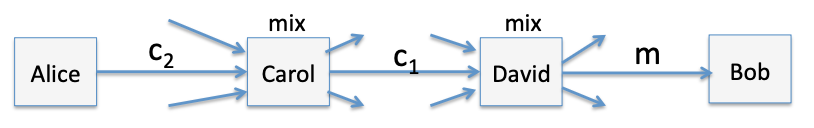
\includegraphics[width=0.6\linewidth]{figures/chapter2/fig7.png}
  \caption{一个使用两层混合的洋葱路由的例子}
  \label{fig:2-7}
\end{figure}

现在,即使 Carol 监测了所有的网络流量,也不能确定谁在 Bob 的论坛上发布了哪条消息。这对 David 来说也是如此。然而,如果 Carol 和 David 是串通的,他们就能搞清楚这些信息。由于这个原因,Alice 可能会通过两个以上的混合网络来传递她的信息。只要其中的一个混合服务不与其他混合服务共谋,Alice 就能够保护她的匿名性。

一个稍微有点复杂的情况是,当 Alice 与 David 建立共享秘钥 $k_{\rm d}$ 时,她不能向 David 透露她的身份。否则,David 就会知道 $c_1$ 来自 Alice,这是我们不希望看到的。这个目标并不难实现,我们将在本书后面介绍如何做到这一点(见 \ref{sec:21-13} 节)。

\begin{snote}[嵌套加密的安全性。]
为了保持Alice的匿名性,知道 $k_{\rm c}$ 的 Carol 不能从式 \ref{eq:2-12} 的嵌套密文 $c_2$ 中获取任何关于 $m$ 的信息。否则,Carol 就有可能利用她从 $c_2$ 中了解到的关于 $m$ 的信息,将 Alice 与她在 Bob 的论坛上发的帖子联系起来。比如说,假设 Carol 可以从 $c_2$ 中了解到 $m$ 的前几个字符,然后她发现 Bob 的论坛上只有一个帖子以这些字符开头。那么 Carol 就可以将整个帖子与 Alice 关联起来,因为她知道 $c_2$ 是来自 Alice 的。

对 David 来说也是如此:知道 $k_{\rm d}$ 的 David 最好无法从式 \ref{eq:2-12} 的嵌套密文 $c_2$ 中得知任何关于 $m$ 的信息。

我们下面论证,如果 $\mathcal{E}$ 是语义安全的,那么在给定 $c_2$ 和 $k_c$ 或 $k_d$ 两个密钥中的一个的情况下,任何有效对手都无法了解任何关于 $m$ 的信息。
\end{snote}

一般地,对于定义在 $(\mathcal{K},\mathcal{M},\mathcal{C})$ 上的密码 $\mathcal{E}=(E,D)$,我们定义 $n$ 层嵌套密码 $\mathcal{E}_n=(E_n,D_n)$ 如下:
\[
E_n\big((k0,\dots,k_{n-1}),\,m\big)=E\big(k_{n-1},E(k_{n-2},\,\cdots E(k_0,m)\cdots\big)
\]
解密算法以相反的顺序使用密钥:
\[
D_n\big((k0,\dots,k_{n-1}),\,c\big)=D\big(k_0,E(k_1,\,\cdots E(k_{n-1},m)\cdots\big)
\]
我们的目标是表明,如果$\mathcal{E}$是语义安全的,那么就算对手得到了除了$k_0,\dots,k_{n-1}$中某一个以外的所有密钥,$\mathcal{E}_n$也是语义安全的。为了更加精确,我们定义两个实验:实验$0$和实验$1$,对于$b=0,1$,实验$b$的工作方式如下:
\begin{itemize}
	\item 对手将 $(m_0,m_1,d)$ 交给挑战者,其中 $m_0,m_1\in\mathcal{M}$ 是长度相等的两条消息,且 $0\leq d<n$。
	\item 挑战者选择 $n$ 个密钥 $k_0,\dots,k_{n-1}\overset{\rm R}\leftarrow\mathcal{K}$ 并计算 $c\overset{\rm R}\leftarrow E_n\big((k_0,\dots,k_{n-1}),\,m_b\big)$。它将 $c$ 和所有的密钥 $k_0,\dots,k_{n-1}$ 一起发送给对手,但不包括密钥 $k_{\rm d}$。
	\item 对手输出一个比特 $\hat b\in\{0,1\}$。
\end{itemize}
这个游戏抓住了这样一个事实:对手得到除 $k_{\rm d}$ 以外的所有密钥 $k_0,\dots,k_{n-1}$,并试图破坏语义安全性。

如同语义安全性的定义,我们定义对手的优势 $\mathrm{NE^{(n)}}\mathsf{adv}[\mathcal{A},\mathcal{E}]$ 如下:
\[
\mathrm{NE^{(n)}}\mathsf{adv}[\mathcal{A},\mathcal{E}]=\big\vert\Pr[W_0]-\Pr[W_1]\big\vert
\]
其中 $W_b$ 是 $\mathcal{A}$ 在实验 $b$ 中输出 $1$ 的事件,对于$b=0,1$,如果 $\mathrm{NE^{(n)}}\mathsf{adv}[\mathcal{A},\mathcal{E}]$ 可忽略不计,我们就说 $\mathcal{E}$ 对于 $n$ 层嵌套是语义安全的。

\begin{theorem}
对于每个常数 $n>0$,如果 $\mathcal{E}=(E,D)$ 是语义安全的,那么 $\mathcal{E}$ 对于 $n$ 层嵌套来说也是语义安全的。
\begin{quote}
特别地,对于每个攻击 $\mathcal{E}_n$ 的 $n$ 层嵌套对手 $\mathcal{A}$,都存在一个攻击 $\mathcal{E}$ 的语义安全对手 $\mathcal{B}$,其中 $\mathcal{B}$ 是围绕 $\mathcal{A}$ 的一个基本包装器,满足:
\end{quote}
\[
\mathrm{NE^{(n)}}\mathsf{adv}[\mathcal{A},\mathcal{E}]=\mathrm{SS}\mathsf{adv}[\mathcal{B},\mathcal{E}]
\]
\end{theorem}

\noindent
这个定理的证明很适合作为安全归约的练习。我们把它留给练习 2.15。
\section{笔记}

一次性密码本由吉尔伯特·弗纳姆于1917年提出,尽管也有证据表明它其实在那之前就已经被发现了。

对文献的引用有待补充。

\section{练习}

\begin{exercise}[乘性一次性密码本]
我们还可以定义一个``乘法模$p$"的一次性密码本变体。这是一个定义在$(\mathcal{K},\mathcal{M},\mathcal{C})$上的密码$\mathcal{E}=(E,D)$,其中$\mathcal{K}:=\mathcal{M}:=\mathcal{C}:=\{1,\dots,p-1\}$,其中$p$是一个素数。加密和解密算法的定义如下:
\[
E(k,m):=k\cdot m \mod p\quad\quad
D(k,c):=k^{-1}\cdot c \mod p
\]
这里,$k^{-1}$表示$k$对$p$的模逆元。验证这个密码的正确性属性,并证明它是完美安全的。
\end{exercise}

\begin{exercise}[一个好的替换密码]
考虑例 \ref{exmp:2-3} 中定义的替换密码 $\mathcal{E}=(E,D)$ 的一个变体,其中消息的每个符号都是用\emph{独立的}置换来加密的。也就是说,令 $\mathcal{M}=\mathcal{C}=\Sigma^L$,其中$\Sigma$是某个有限符号表,$L$是某个长度。令密钥空间为$\mathcal{K}=S^L$,其中$S$是$\Sigma$上所有置换的集合。加密算法$E(k, m)$的定义为:
\[
E(k,m):=\Big(k[0](m[0]),\;k[1](m[1]),\;\dots,\;k[L-1](m[L-1])\Big)
\]
证明$\mathcal{E}$是完美安全的。
\end{exercise}

\begin{exercise}[链式加密]
令$\mathcal{E}=(E,D)$ 是一个定义在$(\mathcal{K},\mathcal{M},\mathcal{C})$上的完美安全密码,其中$\mathcal{K}=\mathcal{M}$。令$\mathcal{E}'=(E',D')$ 是一个密码,其加密算法的定义为 $E'((k_1,k_2),m):=\big(E(k_1,k_2),E(k_2,m)\big)$。证明$\mathcal{E}'$是完美安全的。
\end{exercise}

\begin{exercise}[被破坏的一次性密码本]
考虑一个消息空间为$\{0,1\}^L$的一次性密码本变体,其密钥空间$\mathcal{K}$被限制为所有包含偶数个$1$的$L$比特字符串所构成的集合。给出一个语义安全优势为$1$的有效对手。
\end{exercise}

\begin{exercise}[更强的不可能结果]
这个练习推广了香农定理(定理 \ref{theo:2-5})。令$\mathcal{E}$是一个定义在$(\mathcal{K},\mathcal{M},\mathcal{C})$上的密码。假设$\mathrm{SS}\mathsf{adv}[\mathcal{A},\mathcal{E}]\leq\epsilon$对\emph{所有的}对手$\mathcal{A}$都成立,甚至包括在\emph{计算上无界的}对手。证明$|\mathcal{K}|\geq(1-\epsilon)|\mathcal{M}|$。
\end{exercise}

\begin{exercise}[匹配的边界]
这个练习是对上一个练习的一种逆推。对于$j=0,\dots,L-1$,令$\epsilon=1/2^j$。考虑定义在$(\mathcal{K},\mathcal{M},\mathcal{C})$上的$L$比特一次性密码本变体$\mathcal{E}$,其中$\mathcal{M}=\mathcal{C}=\{0,1\}^L$。密钥空间$\mathcal{K}$被限制为所有前$j$位不全为零的$L$比特字符串所构成的集合,因此 $|\mathcal{K}|=(1-\epsilon)|\mathcal{M}|$。证明:
\begin{enumerate}[\indent(a)]
	\item 存在一个有效对手$\mathcal{A}$,使得$\mathrm{SS}\mathsf{adv}[\mathcal{A},\mathcal{E}]=\epsilon/(1-\epsilon)$;
	\item 对于\emph{所有的}对手$\mathcal{A}$,甚至包括\emph{计算上无界的}对手,都有$\mathrm{SS}\mathsf{adv}[\mathcal{A},\mathcal{E}]\leq\epsilon/(1-\epsilon)$。
\end{enumerate}
\textbf{注意:}由于(a)中$\mathcal{A}$的优势是非零的,所以密码$\mathcal{E}$不可能是完美安全的。
\end{exercise}

\begin{exercise}[确定性密码]
在这个练习中,我们要求你详细证明例 \ref{exmp:2-9} 中的声称。也就是证明,如果$\mathcal{E}$是一个完美安全的确定性密码,那么对于每个对手 $\mathcal{A}$ 都有 $\mathrm{SS}\mathsf{adv}[\mathcal{A},\mathcal{E}]=0$(记住,$\mathcal{A}$ 可能是概率性的);同时证明,如果$\mathcal{E}$是变长一次性密码本, 那么对于所有对手 $\mathcal{A}$ 都有 $\mathrm{SS}\mathsf{adv}[\mathcal{A},\mathcal{E}]=0$。
\end{exercise}

\begin{exercise}[轮盘赌]
在 \ref{subsec:2-2-4} 小节中,我们论证了如果使用语义安全的密码对一个值$r$进行加密,那么玩家在网络轮盘赌中获胜的几率与真实轮盘赌非常接近。然而,我们的``轮盘赌"游戏相当简单。假设我们有一个更复杂的游戏,不同的结果可能会导致不同的赢利。规则并不那么重要,但假设规则很容易评估(给定一个赌注和数字$r$),每个赌注的结果都是$0,1,\dots,n$美元,其中$n$是多项式边界的。令$\mu$是这个游戏的真实版本(没有加密)的最佳策略中的预期赢利。令$\mu'$是这个游戏的网络版本(有加密)中某个(有效)玩家的预期赢利。假设密码是语义安全的,证明$\mu'\leq\mu+\epsilon$,其中$\epsilon$可忽略不计。

	\vspace{3pt}
	
\noindent
\textbf{提示:}你可能需要利用这样一个事实:如果$\mathsf{X}$是一个在$\{0,1,\dots,n\}$中取值的随机变量,那么$\mathsf{X}$的期望等于$\sum_{i=1}^n\Pr[\mathsf{X}\geq i]$。
\end{exercise}

\begin{exercise}
使用 \ref{sec:2-3} 节中的正式定义证明事实 \ref{fact:2-6}。
\end{exercise}

\begin{exercise}[练习语义安全性的定义]
令$\mathcal{E}=(E,D)$是一个定义在$(\mathcal{K},\mathcal{M},\mathcal{C})$上的语义安全密码,其中$\mathcal{M}=\mathcal{C}=\{0,1\}^L$。以下哪种加密算法会产生语义安全的方案?要么给出一种攻击,要么通过明确的归约提供一个安全证明。
\begin{enumerate}[\indent(a)]
	\item $E_1(k,m):=0\;||\;E(k,m)$
	\item $E_2(k,m):=E(k,m)\;||\;\mathrm{parity}(m)$
	\item $E_3(k,m):=\mathrm{reverse}(E(k,m))$
	\item $E_4(k,m):=E(k,\mathrm{reverse}(m))$
\end{enumerate}
这里,对于一个比特串$s$,如果$s$中有奇数个比特$1$,则$\mathrm{parity}(s)$为$1$,否则为$0$;另外,$\mathrm{reverse}(s)$是通过颠倒$s$中比特的顺序得到的字符串,例如,$\mathrm{reverse}(1011)=1101$。
\end{exercise}

\begin{exercise}[密钥恢复攻击]
令$\mathcal{E}=(E,D)$是一个定义在$(\mathcal{K},\mathcal{M},\mathcal{C})$上的密码。密钥恢复攻击用下面的挑战者与对手$\mathcal{A}$之间的游戏建模:挑战者在$\mathcal{K}$中选择一个随机密钥$k$,在$\mathcal{M}$中选择一个随机消息$m$,计算$c\overset{\rm R}\leftarrow E(k,m)$,并将$(m,c)$发送给$\mathcal{A}$。$\mathcal{A}$输出一个$\mathcal{K}$中的猜测值$\hat k$作为应答。如果$D(\hat{k},c)=m$,我们就称$\mathcal{A}$赢得了游戏,并将$\mathcal{A}$赢得游戏的概率定义为$\mathrm{KR}\mathsf{adv}[\mathcal{A},\mathcal{E}]$。和往常一样,如果对于所有有效对手$\mathcal{A}$,优势$KRadv[A,E]$都可忽略不计,我们就说$\mathcal{E}$对于密钥恢复攻击是安全的。
\begin{enumerate}[\indent(a)]
	\item 证明一次性密码本对密钥恢复攻击是不安全的。
	\item 证明如果$\mathcal{E}$是语义安全的,并且$\epsilon=|\mathcal{K}|/|\mathcal{M}|$可忽略不计,那么$\mathcal{E}$对密钥恢复攻击是安全的。特别地,证明对于每个有效的密钥恢复对手$\mathcal{A}$,都存在一个有效的语义安全对手$\mathcal{B}$,其中$\mathcal{B}$是一个围绕$\mathcal{A}$的基本包装器,使得:
	$$\mathrm{KR}\mathsf{adv}[\mathcal{A},\mathcal{E}]\leq\mathrm{SS}\mathsf{adv}[\mathcal{B},\mathcal{E}]+\epsilon$$
	\textbf{提示:}你的语义安全对手$\mathcal{B}$在语义安全实验$0$中会以$\mathrm{KR}\mathsf{adv}[\mathcal{A},\mathcal{E}]$的概率输出$1$,在实验$1$中以最多$\epsilon$的概率输出$1$。由此可以推导出用$\epsilon$表示的$\mathrm{SS}\mathsf{adv}[\mathcal{B},\mathcal{E}]$的下界,并由该结果得到$\mathrm{KR}\mathsf{adv}[\mathcal{A},\mathcal{E}]$。
	\item 基于(b)证明,如果 $\mathcal{E}$ 在是语义安全的,并且$|\mathcal{M}|$是超多项式的,那么$|\mathcal{K}|$不可能是多项式边界的。

	\vspace{1pt}

	\textbf{注意:}当$|\mathcal{M}|$是多项式边界的时候,$|\mathcal{K}|$可以是多项式边界的,比如在一次性密码本中。
\end{enumerate}
\end{exercise}

\begin{exercise}[对消息恢复的安全性]
在 \ref{subsubsec:2-2-3-1} 小节中,我们提出了针对消息恢复的安全性的概念。构建一个对消息恢复安全,但不是语义安全的密码。
\end{exercise}

\begin{exercise}[在简单环境下计算优势]
考虑以下两个实验:实验$0$和实验$1$:
\begin{itemize}
	\item 在实验$0$中,挑战者抛出一枚公平的硬币(即抛出正面和反面的概率都是$1/2$),并将结果发送给对手$\mathcal{A}$。
	\item 在实验$1$中,挑战者总是向对手发送``反面"。
\end{itemize}
对手的目标是区分这两个实验:在每次实验结束时,对手输出一个比特$0$或$1$,作为其对所处实验的猜测。对于$b=0,1$,令$W_b$为实验$b$中对手输出$1$的事件。对手试图使其区分优势:
\[
\big\vert\Pr[W_0]-\Pr[W_1]\big\vert\in[0,1]
\]
最大化。如果这个优势对所有有效对手来说都是可忽略不计的,那么我们就称这两个实验是无法区分的。
\begin{enumerate}[\indent(a)]
	\item 计算下列对手的优势:
	\begin{enumerate}[(i)]
		\item $\mathcal{A}_1$:总是输出$1$。
		\item $\mathcal{A}_2$:忽略挑战者报告的结果,以相等的概率随机输出$0$或$1$。
		\item $\mathcal{A}_3$:如果从挑战者收到``正面",则输出$1$,否则输出$0$。
		\item $\mathcal{A}_4$:如果从挑战者收到``正面",则输出$0$,否则输出$1$。
		\item $\mathcal{A}_5$:如果收到``正面",则输出$1$;如果收到``反面",则以相等的概率随机输出$0$或$1$。
	\end{enumerate}
	\item 区分这两个实验的最大优势是多少?给出解释。
\end{enumerate}
\end{exercise}

\begin{exercise}[置换密码]
考虑一个定义在$(\mathcal{K},\mathcal{M},\mathcal{C})$上的密码$(E,D)$,其中$\mathcal{C}=\mathcal{M}=\{0,1\}^\ell$,$\mathcal{K}$是集合$\{0,\dots,\ell\}$的所有$\ell!$个置换排列的集合。对于密钥$k\in\mathcal{K}$和消息$m\in\mathcal{M}$,定义$E(k,m)$为使用置换$k$对$m$的所有比特进行重排列的结果,即$E(k,m)=m[k(0)]\dots m[k(\ell-1)]$。通过展示一个优势为$1$的对手来证明改密码不是语义安全的。
\end{exercise}

\begin{exercise}[嵌套加密]\label{exer:2-15}
对于一个密码$\mathcal{E}=(E,D)$,定义嵌套密码$\mathcal{E}'=(E',D')$为:
\[
E'\big((k_0,k_1),m\big)=E\big(k_1,E(k_0,m)\big),\quad
D'\big((k_0,k_1),c\big)=D\big(k_0,D(k_1,c)\big)
\]
我们的目标是证明,如果$\mathcal{E}$是语义安全的,那么就算对手得到了$k_0$或$k_1$中的任意一个密钥,$\mathcal{E}'$也是语义安全的。
\begin{enumerate}[\indent(a)]
	\item 考虑以下语义安全实验,即实验$0$和实验$1$:在实验$b$中,对于$b=0,1$,对手产生两条消息$m_0$和$m_1$,并得到$k_1$和$E'\big((k_0,k_1),m_b\big)$。对手输出一个$\{0,1\}$中的值$\hat b$。同之前在语义安全的定义中类似,我们定义对手的优势为 $\mathrm{NE}\mathsf{adv}[\mathcal{A},\mathcal{E}]$。证明对于每个攻击$\mathcal{E}'$的嵌套加密对手$\mathcal{A}$,都存在一个攻击$\mathcal{E}$的语义安全对手$\mathcal{B}$,其中$\mathcal{B}$是一个围绕$\mathcal{A}$的基本包装器,满足:
	\[
	\mathrm{NE}\mathsf{adv}[\mathcal{A},\mathcal{E}]=\mathrm{SS}\mathsf{adv}[\mathcal{B},\mathcal{E}]
	\]
	画一个图,$\mathcal{A}$在右边,$\mathcal{B}$在中间,$\mathcal{B}$的挑战者在左边。在你的安全证明中,展示发生在上述三方之间的信息流。
	\item 如果在(a)中,对手在实验$0$和实验$1$中得到的是$k_0$(而不是$k_1$)和$E'\big((k_0,k_1),m_b\big)$,重复(a)中的证明。像(a)一样,画一张图展示安全证明中的信息流。
\end{enumerate}
这个问题出现在了 \ref{sec:2-4} 节中讨论的互联网匿名路由中。
\end{exercise}

\begin{exercise}[自指加密]
证明用一个密钥加密其自身是危险的。令$\mathcal{E}$是一个定义在$(\mathcal{K},\mathcal{M},\mathcal{C})$上的语义安全密码,其中$\mathcal{K}\subseteq\mathcal{M}$,并令$k\overset{\rm R}\leftarrow\mathcal{K}$。一个密文$c_*:=E(k,k)$,即用$k$加密$k$,被称为\textbf{自指加密(self-referential encryption)}。
\begin{enumerate}[\indent(a)]
	\item 构建一个派生自$\mathcal{E}$的密码$\mathcal{\tilde{E}}=(\tilde{E},\tilde{D})$,使得$\tilde{E}$在是语义安全的,但如果对手得到了$\tilde{E}(k,k)$,则变得不安全。这证明了语义安全并不意味着加密自己的密钥也是安全的。
	\item 构建一个派生自$\mathcal{E}$的密码$\mathcal{\hat{E}}=(\hat{E},\hat{D})$,使得$\hat{E}$是语义安全的,并且即使对手得到了$\hat{E}(k,k)$,也能(被证明)保持语义安全性。为了证明$\hat{E}$是语义安全的,你应该证明:对于每个攻击$\mathcal{\hat{E}}$的对手$\mathcal{A}$,都存在一个攻击$\mathcal{E}$的对手$\mathcal{B}$,使得(i) $\mathcal{B}$的运行时间与$\mathcal{A}$差不多,(ii) $\mathrm{SS}\mathsf{adv}[\mathcal{A},\mathcal{\hat{E}}]\leq\mathrm{SS}\mathsf{adv}[\mathcal{B},\mathcal{E}]$。
\end{enumerate}
\end{exercise}

\begin{exercise}[压缩并加密]
有两个标准委员会提议将压缩与加密相结合以节省带宽(如zip和gzip程序中使用的Lempel-Ziv算法)。这两个委员会都计划使用变长一次性密码本进行加密。
\begin{itemize}
	\item 一个委员会提议先压缩后加密。解释一下为什么这是个坏主意。

	\vspace{1pt}

	\textbf{提示:}回顾一下,压缩可以大大缩减某些消息的大小,而对某些消息的长度影响不大。
	\item 另一个委员会提议先加密后压缩。解释一下为什么这也是个坏主意。
\end{itemize}
多年来,在结合加密和压缩时出现过许多问题。CRIME和BREACH攻击就是很有代表性的例子。
\end{exercise}

\begin{exercise}[投票协议]
这个练习提供了一种基于加性一次性密码本的简易投票协议(例 \ref{exmp:2-4})。假设我们有$t$个投票者和一个计票中心。每个投票者都要投$0$或$1$票,计票中心要统计票数并公布总和$S$。然而,他们将使用一个协议,保证没有任何一方(投票者或计票中心)能知道$S$之外的信息(但我们假定每一方都忠实地遵守该协议)。

该协议的工作方式如下。令$n>t$是一个整数。计票中心产生一个对$0$的加密:$c_0\overset{\rm R}\leftarrow\{0,\dots,n-1\}$,并将 $c_0$ 发送给投票者 $1$。投票者 $1$ 将它的票 $v_1$ 加到 $c_0$ 上,计算 $c_1\leftarrow c_0+v_1 \mod n$,并将 $c_1$ 发送给投票者 $2$。这样继续下去,每个投票者 $i$ 把 $v_i$ 加到 $c_{i-1} $上,计算 $c_i\leftarrow c_{i-1}+v_i \mod n$,并把 $c_i$ 发送给投票者 $i+1$,最后投票者 $t$ 把 $c_t$ 发回计票中心。计票中心计算总和为$S\leftarrow c_t-c_0 \mod n$,并将 $S$ 广播给所有投票者。
\begin{enumerate}[\indent(a)]
	\item 证明该协议能正确计算出总和。
	\item 证明该协议在以下意义上是完美安全的。对于投票者$i=1,\dots,t$,定义$View_i:=(S,c_{i-1})$,它代表投票者$i$的``观点"。我们还定义$View_0:=(c_0,c_t)$代表计票中心的``观点"。证明对于每个$i=0,\dots,t$和$S=0,\dots,t$,以下结论成立:
	\begin{quote}
		无论$v_1,\dots,v_t$的选择如何变化,在$v_j\in\{0,1\}$和$\sum^t_{j=1}v_j=S$的约束下,$View_i$的分布保持不变。
	\end{quote}
	\item 证明如果两个投票者$i$和$j$串通,他们就可以确定第三个投票者$k$的投票。你可以自由选择索引$i$,$j$和$k$。
\end{enumerate}
\end{exercise}

\begin{exercise}[双向分割密钥]
令$\mathcal{E}=(E,D)$是一个定义在$(\mathcal{K},\mathcal{M},\mathcal{C})$上的语义安全密码,其中$\mathcal{K}=\{0,1\}^d$。假设我们希望将解密密文的能力分给两方,比如 Alice 和 Bob。这样,想要解密密文,这两方都必不可少。对于一个$\mathcal{K}$上的随机密钥$k$,随机从$\mathcal{K}$中选择一个$r$并定义$k_a:=r$和$k_b:=k\oplus r$。现在,如果 Alice 和 Bob 在一起,他们就可以重建密钥$k=k_a\oplus k_b$,然后计算$D(k,c)$来解密密文$c$。我们的目标是证明 Alice 和 Bob 都不能单独解密密文。
\begin{enumerate}[\indent(a)]
	\item 构建一个安全概念以捕捉对手在给定 Bob 的密钥 $k_b$ 时打破语义安全性的优势。将这种双向密钥分割优势记为$\mathrm{2KS}\mathsf{adv}[\mathcal{A},\mathcal{E}]$。
	\item 证明对于每一个双向密钥分割对手$\mathcal{A}$,都存在一个语义安全对手$\mathcal{B}$,使得$\mathrm{2KS}\mathsf{adv}[\mathcal{A},\mathcal{E}]=\mathrm{SS}\mathsf{adv}[\mathcal{B},\mathcal{E}]$。
\end{enumerate}
\end{exercise}

\begin{exercise}[简单的秘密共享]\label{exer:2-20}
令$\mathcal{E}=(E,D)$是一个语义安全的密码,密钥空间为$\mathcal{K}=\{0,1\}^L$。一家银行希望将一个解密密钥$k\in\{0,1\}^L$分成$p_0$,$p_1$和$p_2$三份,并且解密至少需要其中的两份。每一份都可以交给不同的银行主管保管,并且每次解密都必须要获得三人中的至少两人的部分。这样一来,即使其中一位高管病休,解密也能进行。
\begin{enumerate}[\indent(a)]
	\item 为了实现这个方案,银行产生两个随机数对$(k_0,k_0')$和$(k_1,k_1')$,它们满足$k_0\oplus k_0'=k_1\oplus k_1'=k$。银行应如何分配密钥份额,才能使得任何两个部分都能用于解密,但任何单独部分都无法完成任务?

	\vspace{1pt}

	\textbf{提示:}第一个执行者得到的部分是$p_0:=(k_0,k_1)$。
	\item 推广(a)的方案,使得解密需要5份中的3份。重组密钥只需要使用各部分的异或。任何两部分都不能透露关于密钥$k$的信息。
	\item 进一步推广,对于任何$t<w$,设计出一个``$w$中选择$t$份"的系统。我们将在 \ref{sec:11-6} 节中看到一个更好的解决该问题的方法。
\end{enumerate}
\end{exercise}

\begin{exercise}[简单的门限解密]
令$\mathcal{E}=(E,D)$是一个语义安全的密码,其密钥空间为$\mathcal{K}$。在这个练习中,我们将设计一个系统,让银行能将一个密钥$k$分成$p_0$,$p_1$和$p_2$三份,并且解密至少需要其中的两份,就像练习 \ref{exer:2-20} 中那样。然而,解密时不需要在一个地方重新组建完整的密钥。

我们使用练习 \ref{exer:2-15} 中介绍的嵌套加密。在$\mathcal{K}^4$中随机选择一个密钥$k:=(k_0,k_1,k_2,k_3)$,并对消息$m$进行加密,即:
\[
c\overset{\rm R}\leftarrow\Big( E\big(k_1,E(k_0,m)\big),\;\,E\big(k_3,E(k_2,m)\big)\Big)
\]
\begin{enumerate}[\indent(a)]
	\item 构建$p_0$,$p_1$和$p_2$的分配方案,使得任何两个部分都能用于解密,但任何单独部分都无法完成任务。

	\vspace{1pt}

	\textbf{提示:}第一个部分是$p_0:=(k_0,k_3)$。
	
	\vspace{1pt}

	\textbf{讨论:}假设持有$p_0$和$p_2$的实体可以进行解密。要解密密文$c$,首先将$c$发送给持有$p_2$的实体以部分解密$c$,然后将结果转发给持有$p_0$的实体以完成解密。这样一来解密就完成了,并不需要在一个地方先组建完整的密钥$k$。
	\item 推广(a)的方案,使得解密需要5份中的3份。解释如何在不重新组合密钥的情况下进行解密。
\end{enumerate}
一种加密方案,如果它的密钥可以被分成若干份,从而使解密需要$w$份中的$t$份,并且解密不需要在单一地点重新装配密钥,就被称为提供\textbf{门限解密(threshold decryption)}。我们将在 \ref{sec:11-6} 节中看到一个更好的解决该问题的方法。
\end{exercise}

\begin{exercise}[偏差校正]
再考虑一下语义安全攻击游戏的比特猜测版本(即攻击游戏 \ref{game:2-4})。假设一个有效对手$\mathcal{A}$能以$1/2+\epsilon$的概率赢得游戏(即猜中隐藏比特$b$),其中$\epsilon$不可忽略不计。请注意,$\epsilon$可以是正数或负数(可忽略不计的定义在绝对值上起作用)。我们的目标是证明存在另一个有效对手$\mathcal{B}$能以$1/2+\epsilon'$的概率赢得游戏,其中$\epsilon'$是一个不可忽略不计的正数。
\begin{enumerate}[\indent(a)]
	\item 考虑以下对手$\mathcal{B}$,它将$\mathcal{A}$作为攻击游戏 \ref{game:2-4} 中的一个子程序,进行以下的两阶段攻击。在第一阶段,$\mathcal{B}$扮演$\mathcal{A}$的挑战者,但$\mathcal{B}$生成自己的隐藏比特$b_0$和自己的密钥$k_0$,最终$\mathcal{A}$输出其猜测比特$\hat b_0$。注意,在这个阶段,$\mathcal{B}$在攻击游戏 \ref{game:2-4} 中的挑战者根本没有参与。在第二阶段,$\mathcal{B}$ 重新启动 $\mathcal{A}$,并让 $\mathcal{A}$ 与攻击游戏 \ref{game:2-4} 中``真正的"挑战者互动,最终 $\mathcal{A}$ 输出一个猜测比特$\hat b$。当这种情况发生时,$\mathcal{B}$ 输出 $\hat{b}\oplus\hat{b}_0\oplus b_0$。请注意,$\mathcal{A}$ 的这次运行完全独立于第一次运行——$\mathcal{A}$ 的硬币和系统参数在这两次运行中是独立产生的。
	
	\vspace{1pt}
	
	证明 $\mathcal{B}$ 赢得攻击游戏 \ref{game:2-4} 的概率为 $1/2+2\epsilon^2$。
	\item 人们可能会倾向于如下论证。只要构造一个运行 $\mathcal{A}$ 的对抗者 $\mathcal{B}$,当 $\mathcal{A}$ 输出 $\hat b$ 时,对手 $\mathcal{B}$ 输出 $\hat{b}\oplus 1$。现在,我们不知道$\epsilon$是正的还是负的。如果它是正的,那么 $\mathcal{A}$ 就满足我们的要求。如果它是负的,那么 $\mathcal{B}$ 就满足我们的要求。虽然我们不知道这两个对手中的哪一个满足我们的要求,但我们知道其中一个肯定满足,所以存在性就被证明了。
	
	\vspace{1pt}
	
	这个论证有什么问题?想要解释这一点,你需要了解有关安全参数的数学细节(见 \ref{sec:2-3} 节)。
	\item 你能想出另一个能以至少 $1/2+|\epsilon|/2$ 的概率赢得比特猜测游戏的有效对手 $\mathcal{B}'$吗?你的对手$\mathcal{B}'$的效率可以比$\mathcal{B}$ 低。
	
	\vspace{1pt}

	\textbf{提示:}尝试多次运行对手 $\mathcal{B}$ 的第一阶段。
\end{enumerate}
\end{exercise}
\chapter{流密码}\label{chap:3}

在上一章中,我们介绍了完美安全加密和语义安全加密的概念。完美安全性的问题在于,想要实现它,我们就必须使用一个很长的密钥。语义安全性旨在提供一个稍弱的安全概念,它允许我们在使用较短密钥的同时构建安全的密码;尽管如此,我们尚未介绍任何满足这个要求的密码。在本章中,我们将考察一类能够实现这一目标的密码:流密码。

\section{伪随机生成器}\label{sec:3-1}

回顾一下,在一次性密码本中,密钥、消息和密文都是 $L$ 比特的序列。然而,我们可能想要使用一个短得多的密钥。我们的想法是,使用一个短的、$\ell$ 比特的``种子" $s$ 作为加密密钥,其中 $\ell$ 比 $L$ 要小得多,然后将这个种子``拉伸"成一个较长的、$L$ 比特的序列,用来掩盖消息(以及解除对密文的掩盖)。拉伸种子 $s$ 需要使用某个有效的确定性算法 $G$,该算法能够将任意 $\ell$ 比特的序列映射为 $L$ 比特的序列。因此,这种修改后的一次性密码本的密钥空间为 $\{0,1\}^\ell$,而消息空间与密文空间仍为 $\{0,1\}^L$。对于 $s\in\{0,1\}^\ell$ 和 $m,c\in\{0,1\}^L$,加密和解密的定义如下:
\[
E(s,m):=G(s)\oplus m,\quad
D(s,c):=G(s)\oplus c
\]
这种修改后的一次性密码本被称作\textbf{流密码(stream cipher)},而函数 $G$ 被称为\textbf{伪随机生成器 (pseudo-random generator)}。

如果 $\ell<L$,那么根据香农定理,这种流密码肯定不能提供完美安全性。但是如果 $G$ 满足适当的安全属性,这种密码仍然可以被视作是语义安全的。假设 $s$ 是一个随机的 $\ell$ 比特序列,$r$ 是一个随机的 $L$ 比特序列。直观地说,如果一个对手无法有效地区分 $G(s)$ 与 $r$,它应该也就无法分辨出这个流密码与一次性密码本之间的区别;此外,既然后者是语义安全的,前者自然也是如此。为了使上述推理更加严谨,我们需要严格定义对手不能``有效区分 $G(s)$ 与 $r$"这一概念。

一种用于区分伪随机序列 $G(s)$ 和真随机序列 $r$ 的算法被称为\textbf{统计检验(statistical test)}。它将一个序列作为输入,并输出 $0$ 或 $1$。如果它在一个伪随机输入上输出 $1$ 的概率和在一个真随机输入上输出 $1$ 的概率之间存在显著的差异,这样的检验就被称作是\textbf{有效的}。即便是相对较小的概率差异,比如说 $1\%$,我们也认为是显著的;事实上,即使只有 $1\%$ 的差异,如果我们能够获得几百个互相独立的样本,而且这些样本要么都是伪随机的,要么都是真随机的,我们就能很有把握地推断出,我们所看到的序列到底是伪随机的,还是真随机的。然而,一个非零但可忽略不计的概率差异,比如 $2^{-100}$,就是没有帮助的。

我们该如何去设计一个有效的统计检验呢?一个基本的方法是:给定一个 $L$ 比特序列,计算某个统计量,然后看看在假设该序列是真随机序列的情况下,这个统计量是否与我们的预期存在较大的差异。

比如说,一个非常简单的、很容易计算的统计量就是二进制序列中比特 $1$ 出现的次数 $k$。对于一个真随机序列,我们期望 $k\approx L/2$。如果 PRG $G$ 对比特 $1$ 或者比特 $0$ 存在某种偏向性,我们就可以通过一个统计检验有效地侦测到这样的偏差。比如说,如果 $|k-0.5L|<0.01L$,我们就输出 $1$,否则输出 $0$。如果 PRG $G$ 确实对 $0$ 或 $1$ 有一些明显的偏向,这个统计检验是就会相当有效。

上面例子中的检验还可以进一步加强,我们不仅可以考虑单个比特,还能够考虑成对的比特。我们可以将 $L$ 比特的序列分解成 $\approx L/2$ 个比特对,并统计数对 $00$ 出现的次数 $k_{00}$,数对 $01$ 出现的次数 $k_{01}$,数对 $10$ 出现的次数 $k_{10}$,以及数对 $11$ 出现的次数 $k_{11}$。对于一个真随机序列,我们期望上面的这四个统计量都 $\approx L/2\cdot 1/4=1/8$。因此,一个自然而然的统计检验就是检验这些统计量与 $L/8$ 之间的偏差是否小于某个特定界限。或者,我们也可以将这些偏差的平方相加,并检验这个和是否小于某个特定界限——这就是统计学中经典的 $\chi$ 方检验。很显然,我们可以从比特对出发,将这个想法进一步推广到任何长度的元组。

我们还可以检查其他的许多简单的统计量。然而,这些简单的检验并不倾向于利用算法 $G$ 的更深层次的数学特性,而后者很可能被恶意对手利用,以设计专门针对 $G$ 的攻击。比如说,对于一些 PRG,上面介绍的两种简单的检验对其完全无效,但当给定足够多的输出比特时,其模式是完全可以预测的;也就是说,给定 $G(s)$ 的一个足够长的前缀,对手就可以计算出 $G(s)$ 的所有剩余比特,甚至能够计算出种子 $s$ 本身。

我们对 PRG 的安全性的定义正式地确定了一个概念,即不应该存在有效的(并且可有效计算的)统计检验。

\subsection{伪随机生成器的定义}\label{subsec:3-1-1}

\textbf{伪随机生成器(pseudo-random generator)},简称\textbf{PRG},是一种有效的确定性算法 $G$,它以一个种子 $s$ 为输入,计算并输出一个值 $r$。种子 $s$ 来自一个有限的\textbf{种子空间} $\mathcal{S}$,而输出 $r$ 属于一个有限的\textbf{输出空间} $\mathcal{R}$。通常情况下,$\mathcal{S}$ 和 $\mathcal{R}$ 是两个比特序列的集合,它们的长度都是被提前规定的(例如,在上面的讨论中,我们有 $\mathcal{S}=\{0,1\}^\ell$ 和 $\mathcal{R}=\{0,1\}^L$)。我们称 $G$ 是一个定义在 $(\mathcal{S},\mathcal{R})$ 上的 PRG。

我们对 PRG 的安全定义抓住了这样一个直观的概念:如果 $s$ 是从 $\mathcal{S}$ 中随机选出的,而 $r$ 是从 $\mathcal{R}$ 中随机选出的,那么任何有效对手都无法有效地分辨 $G(s)$ 和 $r$ 之间的差别:两者是\textbf{计算上不可区分(computationally indistinguishable)}的。我们将该定义表述为一个攻击游戏。

\begin{game}[伪随机生成器]\label{game:3-1}
对于一个定义在 $(\mathcal{S},\mathcal{R})$ 上的给定 PRG $G$ 和一个给定对手 $\mathcal{A}$,我们定义两个实验:实验 $0$ 和实验 $1$。对于 $b=0,1$,我们定义:

\vspace{5pt}

\noindent\textbf{实验 $b$:}
\begin{itemize}
	\item 挑战者按如下方式计算 $r\in\mathcal{R}$:
	\begin{itemize}
		\item 如果 $b=0$:$s\overset{\rm R}\leftarrow\mathcal{S}$,$r\leftarrow G(s)$;
		\item 如果 $b=1$:$r\overset{\rm R}\leftarrow\mathcal{R}$。
	\end{itemize}
	然后将 $r$ 发送给对手。
	\item 给定$r$,对手计算并输出一个比特 $\hat{b}\in\{0,1\}$。
\end{itemize}

对于 $b=0,1$,定义 $W_b$ 是 $\mathcal{A}$ 在实验 $b$ 中输出 $1$ 的事件。我们将 $\mathcal{A}$ 就 $G$ 的\textbf{优势}定义为:
\[
{\rm PRG\mathsf{adv}}[\mathcal{A},G]
:=
\big\lvert
\Pr[W_0]-\Pr[W_1]
\big\rvert
\]
\end{game}

该攻击游戏如图 \ref{fig:3-1} 所示。

\begin{figure}
	\centering
	\input{figures/chapter3/fig1.tex}
	\caption{攻击游戏 \ref{game:3-1} 的实验$0$和实验$1$}
	\label{fig:3-1}
\end{figure}

\begin{definition}[安全的 PRG]\label{def:3-1}
如果对于所有有效对手 $\mathcal{A}$,${\rm PRG\mathsf{adv}}[\mathcal{A},G]$ 的值都可忽略不计,我们就称 PRG $G$ 是\textbf{安全的}。

\end{definition}

正如 \ref{subsec:2-2-5} 小节所讨论的,攻击游戏 \ref{game:3-1} 可以被重构为一个``比特猜测"游戏。此时,挑战者不再进行两个独立的实验,而是随机选择一个 $b\in\{0,1\}$,然后针对对手 $\mathcal{A}$ 运行实验 $b$。在这个游戏中,我们记 $\mathcal{A}$ 的\emph{比特猜测优势} ${\rm PRG\mathsf{adv}}^*[\mathcal{A},G]$ 为 $|\Pr[\hat{b}=b]-1/2|$。\ref{subsec:2-2-5} 小节的推广结论(即式 \ref{eq:2-11})在此也适用:
\begin{equation}
\mathrm{PRG}\mathsf{adv}[\mathcal{A},G]
=2\cdot
\mathrm{PRG}\mathsf{adv}^*[\mathcal{A},G]
\end{equation}

我们还注意到,只有当种子空间的\emph{势 (cardinality)}是超多项式的时候,PRG 才是安全的(见练习 \ref{exer:3-5})。

\subsection{数学细节}\label{subsec:3-1-2}

和 \ref{sec:2-3} 节一样,我们在这里给出更多与 PRG 有关的数学细节。读者在初读这一小节时可以安全地跳过,而不用担心在理解上有什么损失。

首先,我们使用定义 \ref{def:2-9} 中提供的术语来精确地定义 PRG。

\begin{definition}[伪随机生成器]\label{def:3-2}
一个伪随机生成器包含一个算法 $G$,以及两个具有系统参数化 $P$ 的空间族:
\[
\mathbf{S}=\{\mathcal{S}_{\lambda,\Lambda}\}_{\lambda,\Lambda},\quad
\mathbf{R}=\{\mathcal{R}_{\lambda,\Lambda}\}_{\lambda,\Lambda}
\]
满足:
\begin{enumerate}
	\item $\mathbf{S}$ 和 $\mathbf{R}$ 是可有效识别和采样的。
	\item 算法 $G$ 是一个有效的确定性算法,对于输入 $\lambda,\Lambda,s$,其中 $\lambda\in\mathbb{Z}_{\geq1}$,$\Lambda\in{\rm Supp}(P(\lambda))$,$s\in\mathcal{S}_{\lambda,\Lambda}$,它输出 $\mathcal{R}_{\lambda,\Lambda}$ 中的一个元素。
\end{enumerate}
\end{definition}

接下来,我们需要对定义 \ref{def:3-1} 进行正确的解释。首先,在攻击游戏 \ref{game:3-1} 中,读者需要理解,对于安全参数 $\lambda$ 的每个可能取值,我们都能得到一个不同的概率空间,该空间由挑战者的随机选择和对手的随机选择共同决定。其次,挑战者会产生一个系统参数 $\Lambda$,并在游戏一开始时将其发送给对手。第三,优势 ${\rm PRG\mathsf{adv}}[\mathcal{A},G]$ 是安全参数 $\lambda$ 的一个函数,而安全性意味着,该函数是一个可忽略不计函数。
\section{流密码:使用 PRG 进行加密}\label{sec:3-2}

令 $G$ 是一个定义在 $(\{0,1\}^\ell,\{0,1\}^L)$ 上的 PRG;也就是说,$G$ 将一个 $\ell$ 比特的种子拉伸为一个 $L$ 比特的输出。由 $G$ 构建的\textbf{流密码} $\mathcal E=(E,D)$ 定义在 $(\{0,1\}^\ell,\{0,1\}^{\leq L},\{0,1\}^{\leq L})$ 上;对于 $s\in\{0,1\}^\ell$ 和 $m,c\in\{0,1\}^{\leq L}$,加密和解密定义如下:如果 $|m|=v$,则:
\[
E(s,m)=G(s)[0\dots v-1]\oplus m
\]
如果 $|c| = v$,则:
\[
D(s,c)=G(s)[0\dots v-1]\oplus c
\]
读者很容易验证,上述加解密方案能够满足我们对密码的定义(特别是满足了正确性属性)。

请注意,为了分析 $\mathcal E$ 的语义安全性,在攻击游戏 \ref{game:2-1} 中与信息 $m$ 相关的长度就是$m$的自然比特长度 $|m|$。此外还需注意,如果 $v$ 比 $L$ 小得多,那么对于许多实际的 PRG 来说,计算 $G(s)$ 的前 $v$ 位有可能比计算出 $G(s)$ 的所有位然后截断要快得多。

本节的主要结论如下:

\begin{theorem}\label{theo:3-1}
如果 $G$ 是一个安全的 PRG,那么由 $G$ 构建的流密码 $\mathcal E$ 就是一个语义安全的密码。
\begin{quote}
特别地,对于每个如攻击游戏 \ref{game:2-1} 中那样攻击 $\mathcal E$ 的 SS 对手 $\mathcal A$,都存在一个如攻击游戏 \ref{game:3-1} 中那样攻击 $G$ 的 PRG 对手 $\mathcal B$,其中 $\mathcal B$ 是一个围绕 $\mathcal A$ 的基本包装器,满足:
\end{quote}
\begin{equation}\label{eq:3-2}
{\rm SS\mathsf{adv}}[\mathcal{A},\mathcal{E}]=2\cdot{\rm PRG\mathsf{adv}}[\mathcal{B},G]
\end{equation}
\end{theorem}

\begin{proof}[证明思路]
基本思想是,我们可以用一个真随机字符串来替换 PRG 的输出,而不会使得对手的优势增长超过一个不可忽略不计的量。然而,在进行这种替换后,对手的优势为零。
\end{proof}

\begin{proof}
令 $\mathcal A$ 是一个如攻击游戏 \ref{game:2-1} 中那样的攻击 $\mathcal E$ 的有效对手。我们想要证明,如果 $G$ 是一个安全的 PRG,那么 ${\rm SS\mathsf{adv}}[\mathcal{A},\mathcal{E}]$ 可以忽略不计。用语义安全攻击游戏的比特猜测版本更为方便。我们证明:
\begin{equation}\label{eq:3-3}
{\rm SS\mathsf{adv}}^∗[\mathcal{A},\mathcal{E}]={\rm PRG\mathsf{adv}}[\mathcal{B},G]
\end{equation}
对于某个有效对手$\mathcal{B}$成立。那么式 \ref{eq:3-2} 就可以由定理 \ref{theo:2-10} 推出。此外,由于我们假设 $G$ 是一个安全的 PRG,那么 ${\rm PRG\mathsf{adv}}[\mathcal{B},G]$ 的值一定是可忽略不计的,因此 ${\rm SS\mathsf{adv}}[\mathcal{A},\mathcal{E}]$ 也是可忽略不计的。

所以,考虑对手 $\mathcal A$ 在攻击游戏 \ref{game:2-1} 的比特猜测版本中对 $\mathcal E$ 的攻击。在这个游戏中,$\mathcal{A}$ 向挑战者提供两个相同长度的消息 $m_0$ 和 $m_1$,然后挑战者选择一个随机密钥 $s$ 和一个随机比特 $b$,并在 $s$ 下对 $m_b$ 进行加密,将得到的密文 $c$ 交给 $\mathcal{A}$;最后,$\mathcal A$ 输出一个比特 $\hat b$。如果 $\hat b=b$,则对手 $\mathcal A$ 赢得游戏。

让我们称这个游戏为\textbf{游戏 $\mathbf{0}$}。 挑战者在这个游戏中的逻辑可以表示如下:

\vspace*{5pt}

\hspace*{5pt} 当收到来自 $\mathcal A$ 的 $m_0,m_1\in\{0,1\}^v$,其中$v\leq L$时:\\
\hspace*{50pt} 计算 $b\overset{\rm R}\leftarrow\{0,1\}$\\
\hspace*{50pt} 计算 $s\overset{\rm R}\leftarrow\{0,1\}^l$,$r\leftarrow G(s)$\\
\hspace*{50pt} 计算 $c\leftarrow r[0\dots v-1]\oplus m_b$\\
\hspace*{50pt} 将 $c$ 发送给 $\mathcal A$。

\vspace*{5pt}

\noindent
图 \ref{fig:3-2} 展示了游戏 $0$ 的流程。

\begin{figure}
	\centering
	\input{figures/chapter3/fig2.tex}
	\caption{定理 \ref{theo:3-1} 的证明中的游戏 $0$}
	\label{fig:3-2}
\end{figure}

记 $W_0$ 为游戏 $0$ 中 $\hat b=b$ 的事件。根据定义,我们有:
\begin{equation}\label{eq:3-4}
{\rm SS\mathsf{adv}}^∗[\mathcal{A},\mathcal{E}]=|\Pr[W_0]-{1}/{2}|
\end{equation}

接下来,我们修改游戏 $0$ 中挑战者的逻辑,得到一个新的游戏,我们称之为\textbf{游戏 $\mathbf{1}$}。游戏 $1$ 与游戏 $0$基本相同,只是挑战者现在会用一个真随机字符串代替伪随机字符串。游戏 $1$ 中挑战者的逻辑如下:

\vspace*{5pt}

\hspace*{5pt} 当收到来自 $\mathcal A$ 的 $m_0,m_1\in\{0,1\}^v$,其中$v\leq L$时:\\
\hspace*{50pt} 计算 $b\overset{\rm R}\leftarrow\{0,1\}$\\
\hspace*{47pt} \colorbox{gray!50}{计算 $r\overset{\rm R}\leftarrow\{0,1\}^L$}\\
\hspace*{50pt} 计算 $c\leftarrow r[0\dots v-1]\oplus m_b$\\
\hspace*{50pt} 将 $c$ 发送给 $\mathcal A$。

\vspace*{5pt}

与之前一样,$\mathcal A$ 在该游戏结束时输出一个比特 $\hat b$。我们用灰色强调了和游戏$0$之间的差别。图 \ref{fig:3-3} 展示了游戏$1$的流程。

\begin{figure}
	\centering
	\input{figures/chapter3/fig3.tex}
	\caption{定理 \ref{theo:3-1} 的证明中的游戏 $1$}
	\label{fig:3-3}
\end{figure}

记 $W_1$ 为游戏 $1$ 中 $\hat b=b$ 的事件。我们声称:
\begin{equation}\label{eq:3-5}
\Pr[W_1]={1}/{2}
\end{equation}
这是因为在游戏 $1$ 中,对手事实上攻击的是变长一次性密码本。特别地,很容易看到,对手的输出 $\hat b$ 和挑战者的隐藏比特 $b$ 是相互独立的。

最后,我们展示如何构建一个有效 PRG 对手 $\mathcal B$,它将 $\mathcal A$ 作为一个子程序,使得:
\begin{equation}\label{eq:3-6}
|\Pr[W_0]-\Pr[W_1]|={\rm PRG\mathsf{adv}}[\mathcal{B},G]
\end{equation}
成立。这实际上非常简单。我们的新对手 $\mathcal B$ 的逻辑如图 \ref{fig:3-4} 所示。这里,$\delta$的定义如下:
\begin{equation}\label{eq:3-7}
\delta(x,y)=
\left\{
\begin{array}{ll}
1, & x=y\\
0, & x\neq y
\end{array}
\right.
\end{equation}
另外,标有``PRG 挑战者"的方框扮演攻击游戏 \ref{game:3-1} 中 $G$ 的挑战者的角色。

\begin{figure}
	\centering
	\input{figures/chapter3/fig4.tex}
	\caption{定理 \ref{theo:3-1} 的证明中的PRG对手$\mathcal{B}$}
	\label{fig:3-4}
\end{figure}

换句话说,对手 $\mathcal B$ 是一个(如攻击游戏 \ref{game:3-1} 中那样)旨在攻击 $G$ 的 PRG 对手,它从它的 PRG 挑战者那里收到 $r\in\{0,1\}^L$,然后扮演 $\mathcal A$ 的挑战者角色,如下所示:

\vspace*{5pt}

\hspace*{5pt} 当收到来自 $\mathcal A$ 的 $m_0,m_1\in\{0,1\}^v$,其中$v\leq L$时:\\
\hspace*{50pt} 计算 $b\overset{\rm R}\leftarrow\{0,1\}$\\
\hspace*{50pt} 计算 $c\leftarrow r[0\dots v-1]\oplus m_b$\\
\hspace*{50pt} 将 $c$ 发送给 $\mathcal A$。

\vspace*{5pt}

\noindent
最后,当 $\mathcal A$ 输出一个比特 $\hat b$ 时,$\mathcal B$ 输出比特 $\delta(\hat b,b)$。

令 $p_0$ 为 PRG 挑战者在运行攻击游戏 \ref{game:3-1} 的实验 $0$ 时,$\mathcal B$ 输出 $1$ 的概率,令 $p_1$ 为 PRG 挑战者运行攻击游戏 \ref{game:3-1} 的实验 $1$ 时,对手 $\mathcal B$ 输出 $1$ 的概率。根据定义,${\rm PRG\mathsf{adv}}[\mathcal{A},G]=|p_1-p_0|$。此外,如果 PRG 挑战者正在运行实验 $0$,那么对手 $\mathcal A$ 本质上就是在进行我们这里的游戏 $0$,所以有 $p_0=\Pr[W_0]$;而如果 PRG 挑战者正在进行实验  $1$,那么对手 $\mathcal A$ 本质上就是在进行我们这里的游戏 $1$,所以有$p_1=\Pr[W_1]$。于是我们立即就能得到式 \ref{eq:3-6}。

结合式 \ref{eq:3-4},\ref{eq:3-5} 和 \ref{eq:3-6},我们就可得到式\ref{eq:3-3}。
\end{proof}

在上述定理中,我们将 $\mathcal E$ 的安全性归约到 $G$ 的安全性上,并表明如果 $\mathcal A$ 是一个攻击 $\mathcal E$ 的有效语义安全对手,那么存在一个攻击 $G$ 的有效 PRG 对手 $\mathcal B$,使得:
\[
{\rm SS\mathsf{adv}}[\mathcal{A},\mathcal{E}]\leq 2\cdot{\rm PRG\mathsf{adv}}[\mathcal{B},G]
\]
(实际上,我们还证明了等号是成立的,但这并不重要。)在证明中,我们认为如果 $G$ 是安全的,那么 ${\rm PRG\mathsf{adv}}[\mathcal{B},G]$ 的值可忽略不计。因此,根据上述不等式,我们得出结论,${\rm SS\mathsf{adv}}[\mathcal{A},\mathcal{E}]$ 也是可忽略不计的。由于这对所有的有效对手 $\mathcal A$ 都成立,于是我们可以得出结论,$\mathcal E$ 是语义安全的。

类似于定理 \ref{theo:2-7} 之后的讨论,另一种结构化的证明方法是反证法:事实上,如果我们假设 $\mathcal E$ 是不安全的,那么一定有一个有效对手 $\mathcal A$ 能使得 ${\rm SS\mathsf{adv}}[\mathcal{A},\mathcal{E}]$ 的值不可忽略不计。而安全归约(以及上述不等式)赋予我们一个有效对手 $\mathcal B$,使得 ${\rm PRG\mathsf{adv}}[\mathcal{B},G]$ 的值也不可忽略不计。也就是说,如果我们能破解 $\mathcal E$,我们也就能破解 $G$。虽然这在逻辑上是等价的,但这样的证明有一种不同的``感觉":我们从破解 $\mathcal E$ 的对手 $\mathcal A$ 开始,并说明如何使用 $\mathcal A$ 来构造一个能破解 $G$ 的新对手 $\mathcal B$。

读者应该注意到,上述定理的证明与我们在 \ref{subsec:2-2-4} 小节中对网络电子轮盘赌的分析遵循基本相同的模式。在这两种情况下,我们都从一个攻击游戏开始(图 \ref{fig:2-2} 和图 \ref{fig:3-2}),我们对其进行修改,从而得到一个新的攻击游戏(图 \ref{fig:2-3} 和图 \ref{fig:3-3});而在这个新的攻击游戏中,计算对手的优势非常容易。此外,我们还使用了一个适当的安全假设,以证明对手在原始游戏和修改后的游戏中的优势差异是可忽略不计的。这是通过引入一个新的对手(图 \ref{fig:2-4} 和图 \ref{fig:3-4})来实现的,该对手攻击底层的密码学原语(密码或 PRG),其优势等于这一差异。假设底层原语是安全的,那么这个差异一定是可忽略不计的;或者,我们可以反过来说:如果这个差异是不可忽略不计的,那么新对手就会``破坏"底层密码学原语。

这是一个将在本文中反复出现的模式。因此读者应该仔细研究这种两种分析方法,以确保能够完全理解其中的原理。
\section{流密码的局限性:对一次性密码本的攻击}

尽管流密码是语义安全的,但它们非常脆弱。如果使用不当,它们就会完全丧失安全性。

\subsection{两次密码本是不安全的}

一个流密码可以很好地加密从 Alice 到 Bob 的\emph{单一}消息。然而,Alice 可能希望向 Bob 发送多条消息。简单起见,假设 Alice 希望对两条消息 $m_1$ 和 $m_2$ 进行加密。一个简陋的方案是是使用相同的密钥 $s$ 来加密这两条消息:
\begin{equation}\label{eq:3-8}
c_1\leftarrow m_1\oplus G(s),\quad
c_2\leftarrow m_2\oplus G(s)
\end{equation}
读者稍加思考就会发现,这个构造根本就不安全。一个对手如果能够截获 $c_1$ 和 $c_2$,就能计算出:
\[
\Delta
:=c_1\oplus c_2
=\big(m_1\oplus G(s)\big)\oplus\big(m_2\oplus G(s)\big)
=m_1\oplus m_2
\]
并得到 $m_1$ 和 $m_2$ 的异或。考虑到英文文本中往往会包含足够多的冗余,因此给定 $\Delta=m_1\oplus m_2$,对手就能轻易地恢复出 $m_1$ 和 $m_2$。因此,只要能够获得足够长的密文,式 \ref{eq:3-8} 中的构造就会泄露明文。

式 \ref{eq:3-8} 中的构造被戏称为\textbf{两次密码本(two-time pad)}。我们在上面论证了两次密码本是完全不安全的,特别是,\textbf{一个流密码的密钥不应该被用来加密多条消息}。在本书的很多实例中,使用一次性密码本就足以满足需求。例如像在 \ref{subsec:5-4-1} 小节中,我们将为每条消息选择一个新的随机密钥。然而,在一条密钥可能会被多次使用的环境中,我们绝不能直接使用流密码。我们会在第\ref{chap:5}章构建可以多次使用的密码。

不正确地重复使用流密码密钥是已部署系统中的一个常见错误。例如,一个叫做 PPTP 的协议能够让 $A$ 和 $B$ 两方互相发送加密消息。微软在 Windows NT 中使用了一种叫做 RC4 的流密码来实现 PPTP 协议。在微软最初的实现中,从 $B$ 到 $A$ 的加密密钥与从 $A$ 到 $B$ 的加密密钥是完全相同的 \cite{schneier1998cryptanalysis}。因此,只要窃听到两条方向相反的加密信息,攻击者就可以恢复这两条消息的明文。

另一个关于两次密码本的有趣故事来自 Klehr 的转述,他非常详细地描述了二战期间在美国的俄罗斯间谍是如何使用一次性密码本把消息送回莫斯科的 \cite{haynes1999venona}。正如 Klehr 所解释的,该系统存在一个致命的缺陷:
\begin{quote}
在二战期间,苏联无法生产足够多的一次性密码本 $\dots$ 来满足庞大的密码需求 $\dots$。因此,他们把一些一次性密码本用了两次,还认为这不会损害他们的系统。美国的反间谍部门收集了所有进出美国的国际电报。从 1946 年开始,在英国人的帮助下,他们开始大力破解苏联的信息,由于 $\dots$ 苏联把一些一次性密码本当作两次密码本使用的错误,在接下来的 25 年里,它们破获了大约 2,900 条消息,包含 1941 年至 1946 年(苏联在此期间改用另外一套系统)之间发送的 5,000 多页共计数十万条消息。
\end{quote}
解密工作的代号为 Venona 计划。Venona 计划因揭发了 Julius Rosenberg 和 Ethel Rosenberg 夫妇而声名鹊起,他们参与苏联间谍集团的证据被 Venona 计划完整地揭露出来。从 1995 年开始,所有 3,000 多份由 Venona 计划解密的消息都被公开了。

\subsection{一次性密码本是易被控制的}

语义安全性尽管能够确保对手无法读取明文,却无法提供完整性的保证。在使用流密码时,对手可以改变密文,而这种修改永远不会被解密者发现。更糟糕的是,我们将表明,通过改变密文,攻击者甚至可以控制解密后的明文。

假设攻击者截获了一条密文 $c:=E(s,m)=m\oplus G(s)$。攻击者将 $c$ 改为 $c':=c\oplus\Delta$,其中的 $\Delta$ 是攻击者选取的某个值。因此,解密者收到修改后的消息:
\[
D(s,c')
=c'\oplus G(s)
=(c\oplus\Delta)\oplus G(s)
=m\oplus\Delta
\]
因此,即使攻击者不知道 $m$ 或 $s$,它也能将解密后的消息变成 $m\oplus\Delta$,而 $\Delta$ 是由攻击者选择的。我们称流密码是\textbf{易被控制的(malleable)},因为攻击者可以对明文造成可预测的变化。我们将在第\ref{chap:9}章构建能够同时提供机密性和完整性的密码。

易被控制性可以帮助攻击者的一个简单的案例是加密文件系统。为了具体说明这一问题,假设 Bob 是一位教授,Alice 和 Molly 是两个学生。Bob 的学生通过电子邮件提交他们的作业,然后 Bob 将这些电子邮件存储在一个用流密码加密的磁盘上。一封电子邮件总是以一个标准头部开始。简化一下,我们可以假设一封来自 Alice 的电子邮件总是以 \texttt{From:Alice} 为开头。

现在,假设 Molly 能够进入 Bob 的磁盘,并找到 Alice 发出的,包含她的作业的电子邮件密文。那么,Molly 就可以窃取 Alice 的作业,方法如下。她只需将适当的五字符序列异或到密文的第 $6$ 至 $10$ 位,以将邮件头部的 \texttt{From:Alice} 改为 \texttt{From:Molly}。Molly 只需要对密文进行操作,并且不需要知道 Bob 的私钥。Bob 永远不会知道文件被修改过,当他给 Alice 的作业打分时,还以为这份作业是 Molly 交的。这样,Molly 就窃取了 Alice 的成果。

当然,为了让这种攻击生效,Molly 必须能以某种方式在 Bob 的加密磁盘上找到 Alice 的电子邮件。然而,在加密文件系统的一些具体实现中,文件的元数据(如文件名、修改时间等)是不会被加密的。有了这些元数据,Molly 就可以直接找到 Alice 的加密邮件并进行攻击了。
\section{组合 PRG}

在本节中,我们将讨论两种构造,以允许我们基于旧的 PRG 建立新的 PRG。这些构造允许我们扩展原始 PRG 的输出空间的大小,同时保留其安全性。更重要的是,在本节中我们将介绍一种非常重要的论证技术,称为\textbf{混合论证 (hybrid argument)},该技术在现代密码学中的应用非常广泛。

\subsection{一种并行构造}\label{subsec:3-4-1}

令 $G$ 是一个定义在 $(\mathcal S,\mathcal R)$ 上的 PRG。假设在某些应用中,我们想多次使用 $G$。我们希望$G$的所有输出与$\mathcal{\rm R}$上的随机元素是计算上无法区分的。如果 $G$ 是一个安全的 PRG,并且种子是独立产生的,那么这样的$G$就能满足这个要求。

我们可以将 $G$ 的多个应用建模为一个新的 PRG $G'$。也就是说,我们构建一个新的PRG $G'$,它将$G$应用于$n$个种子,并将输出连接起来。因此,$G'$定义在 $(\mathcal S^n,\mathcal R^n)$ 上,对于 $s_1,\dots,d_n\in\mathcal S$,我们有:
$$
G'(s_1,\dots,s_n):=\big(G(s_1),\dots,G(s_n)\big)
$$
我们称 $G'$ 为 $G$ 的 \textbf{$n$ 次并行组合 ($n$-wise parallel composition)},$n$ 称为\textbf{重复参数 (repetition parameter)},并且,我们要求$n$是一个多项式边界的值。

\begin{theorem}\label{theo:3-2}
如果 $G$ 是一个安全的 PRG,那么 $G$ 的 $n$ 次并行组合 $G'$ 也是一个安全的 PRG。
\begin{quote}
特别地,对于每一个如攻击游戏 \ref{game:3-1} 中那样攻击 $G'$ 的 PRG 对手 $\mathcal A$,都存在一个如攻击游戏 \ref{game:3-1} 中那样攻击 $G$ 的 PRG 对手 $\mathcal B$,其中 $\mathcal B$ 是围绕 $\mathcal A$ 的一个基本包装器,满足:
\end{quote}
$$
{\rm PRG\mathsf{adv}}[\mathcal{A},G']=n\cdot{\rm PRG\mathsf{adv}}[\mathcal{B},G]
$$
\end{theorem}

作为热身,我们首先在 $n=2$ 的特殊情况下证明这个定理。令 $\mathcal A$ 是一个有效 PRG 对手,在攻击游戏 \ref{game:3-1} 中攻击 $G'$ 时有优势 $\epsilon$。我们想证明,如果 $G$ 是一个安全 PRG,则 $\epsilon$ 可以忽略不计。为此,我们把\textbf{游戏 $\mathbf{0}$} 定义为攻击游戏 \ref{game:3-1} 中的实验 $0$。这个游戏中的挑战者的工作方式如下:

\vspace*{5pt}

\hspace*{5pt} 计算 $s_1\overset{\rm R}\leftarrow\mathcal S$,$r_1\leftarrow G(s_1)$\\
\hspace*{26pt} 计算 $s_2\overset{\rm R}\leftarrow\mathcal S$,$r_2\leftarrow G(s_2)$\\
\hspace*{26pt} 将 $(r_1,r_2)$ 发送给 $\mathcal A$。

\vspace*{5pt}

\noindent
令 $p_0$ 为 $\mathcal A$ 在该游戏中输出 $1$ 的概率。

下面,我们定义\textbf{游戏$\mathbf{1}$},它在 $\mathcal A$ 和一个挑战者之间进行,其工作方式如下:

\vspace*{5pt}

\hspace*{2pt} \colorbox{gray!50}{计算 $r_1\overset{\rm R}\leftarrow\mathcal R$}\\
\hspace*{26pt} 计算 $s_2\overset{\rm R}\leftarrow\mathcal S$,$r_2\leftarrow G(s_2)$\\
\hspace*{26pt} 将 $(r_1,r_2)$ 发送给 $\mathcal A$。

\vspace*{5pt}

\noindent
请注意,游戏 $1$ 既不对应于攻击游戏 \ref{game:3-1} 中的实验 $0$,也不对应于实验 $1$;相反,它是一个``混合"实验,对应于实验$0$和实验$1$之间的某个状态。 我们所做的就是在游戏 $0$ 中用一个真随机值取代伪随机值 $r_1$(见上面的高亮行)。直观地说,在假设 $G$ 是一个安全 PRG 的情况下,对手 $\mathcal A$ 应该注意不到这种差异。为了更精确地论证这一点,令 $p_1$ 是 $\mathcal A$ 在游戏 $1$ 中输出 $1$ 的概率。

令 $\delta_1:=|p_1-p_0|$。我们声称,假设 $G$ 是一个安全的 PRG,则 $\delta_1$ 是可忽略不计的。事实上,我们很容易构建一个有效 PRG 对手 $\mathcal B_1$,他在攻击游戏 \ref{game:3-1} 中攻击 $G$ 的优势正好等于 $\delta_1$。对手 $\mathcal B_1$ 的工作方式如下:

\vspace*{5pt}

\hspace*{5pt} 当收到来自挑战者的 $r\in\mathcal R$,$\mathcal B_1$ 扮演 $\mathcal A$ 的挑战者的角色:\\
\hspace*{50pt} 令 $r_1\leftarrow r$\\
\hspace*{50pt} 计算 $s_2\overset{\rm R}\leftarrow\mathcal S$,$r_2\leftarrow G(s_2)$\\
\hspace*{50pt} 将 $(r_1,r_2)$ 发送给 $\mathcal A$。\\
\hspace*{26pt} 最后,$\mathcal B_1$ 输出 $\mathcal A$ 所输出的任何东西。

\vspace*{5pt}

\noindent
请注意,当 $\mathcal B_1$ 在其攻击游戏的实验 $0$ 中时,它完全模仿挑战者在游戏 $0$ 中的行为,而在实验 $1$ 中,它完全模仿挑战者在游戏 $1$ 中的行为。因此,$p_0$ 等于 $\mathcal B_1$ 在攻击游戏 \ref{game:3-1} 的实验 $0$ 中输出 $1$ 的概率,而 $p_1$ 等于 $\mathcal B_1$ 在攻击游戏 \ref{game:3-1} 的实验 $1$ 中输出 $1$ 的概率。因此,$\mathcal B_1$ 在攻击 $G$ 时的优势恰好是 $|p_1-p_0|$,正如我们上面声称的。

接下来,我们定义\textbf{游戏$\mathbf{2}$},它在 $\mathcal A$ 和一个挑战者之间进行,其工作方式如下:

\vspace*{5pt}

\hspace*{5pt} 计算 $r_1\overset{\rm R}\leftarrow\mathcal R$\\
\hspace*{23pt} \colorbox{gray!50}{计算 $r_2\overset{\rm R}\leftarrow\mathcal R$}\\
\hspace*{26pt} 将 $(r_1,r_2)$ 发送给 $\mathcal A$。

\vspace*{5pt}

\noindent
我们所做的就是把游戏 $1$ 中的伪随机值 $r_2$ 替换成一个真正的随机值(见上面的高亮行)。令 $p_2$ 为 $\mathcal A$ 在游戏 $2$ 中输出 $1$ 的概率。请注意,游戏 $2$ 对应于攻击游戏 \ref{game:3-1} 的实验 $1$,因此 $p_2$ 等于攻击游戏 \ref{game:3-1} 的实验 $1$ 中 $\mathcal A$ 相对于 PRG $G'$ 输出 $1$ 的概率。

令 $\delta_2:=|p_2-p_1|$。通过与上面类似的论证,很容易看到当 $G$ 是一个安全的 PRG 时,$\delta_2$ 是可忽略不计的。事实上,我们很容易构建一个有效 PRG 对手 $\mathcal B_2$,他在攻击游戏 \ref{game:3-1} 中攻击 $G$ 的优势正好等于 $\delta_2$。对手 $\mathcal B_2$ 的工作方式如下:

\vspace*{5pt}

\hspace*{5pt} 当收到来自挑战者的 $r\in\mathcal R$,$\mathcal B_2$ 扮演 $\mathcal A$ 的挑战者的角色:\\
\hspace*{50pt} 计算 $r_1\overset{\rm R}\leftarrow\mathcal R$\\
\hspace*{50pt} 令 $r_2\leftarrow r$\\
\hspace*{50pt} 将 $(r_1,r_2)$ 发送给 $\mathcal A$。\\
\hspace*{26pt} 最后,$\mathcal B_2$ 输出 $\mathcal A$ 所输出的任何东西。

\vspace*{5pt}

\noindent
$p_1$ 显然就等于 $\mathcal B_2$ 在攻击游戏 \ref{game:3-1} 的实验 $0$ 中输出 $1$ 的概率,而 $p_2$ 等于 $\mathcal B_2$ 在攻击游戏 \ref{game:3-1} 的实验 $1$ 中输出 $1$ 的概率。

回顾一下,我们有$\epsilon={\rm PRG\mathsf{adv}}[\mathcal{A},G']$,那么从上面的讨论中,我们有:
$$
\epsilon=|p_2-p_0|=|p_2-p_1+p_1-p_0|\leq|p_1-p_0|+|p_2-p_1|=\delta_1+\delta_2
$$
由于 $\delta_1$ 和 $\delta_2$ 都可忽略不计,那么$\epsilon$ 也可忽略不计(见事实 \ref{fact:2-6})。

这就完成了 $G'$ 在 $n=2$ 情况下的安全证明。在给出一般情况下的证明之前,我们先给出 $n=2$ 情况下的另一种证明方式。我们的第一个证明采用了构建两个对手 $\mathcal B_1$ 和 $\mathcal B_2$ 的方法,而第二个证明会把这两个对手合并为一个单一的如同攻击游戏 \ref{game:3-1} 中攻击 $G$ 的 PRG 对手 $\mathcal B$,其工作方式如下:

\vspace*{5pt}

\hspace*{5pt} 当收到来自挑战者的 $r\in\mathcal R$ 时,$\mathcal B$ 进行以下操作:\\
\hspace*{50pt} 随机选取 $\omega\in\{1,2\}$\\
\hspace*{50pt} 将 $r$ 发送给 $\mathcal B_\omega$。\\
\hspace*{26pt} 最后,$\mathcal B$ 输出 $\mathcal B_\omega$ 所输出的任何东西。

\vspace*{5pt}

记 $W_0$ 为 $\mathcal B$ 在攻击游戏 \ref{game:3-1} 的实验 $0$ 中输出 $1$ 的事件,$W_1$ 为 $\mathcal B$ 在攻击游戏 \ref{game:3-1} 的实验 $1$ 中输出 $1$ 的事件。以 $\omega=1$ 和 $\omega=2$ 为条件,我们有:
$$
\begin{aligned}
\Pr[W_0]
&=\Pr[W_0\,|\,\omega=1]\Pr[\omega=1]+\Pr[W_0\,|\,\omega=2]\Pr[\omega=2]\\
&=\frac{1}{2}\Big(\Pr[W_0\,|\,\omega=1]+\Pr[W_0\,|\,\omega=2]\Big)\\
&=\frac{1}{2}(p_0+p_1)
\end{aligned}
$$
类似地,我们也有:
$$
\begin{aligned}
\Pr[W_1]
&=\Pr[W_1\,|\,\omega=1]\Pr[\omega=1]+\Pr[W_1\,|\,\omega=2]\Pr[\omega=2]\\
&=\frac{1}{2}\Big(\Pr[W_1\,|\,\omega=1]+\Pr[W_1\,|\,\omega=2]\Big)\\
&=\frac{1}{2}(p_1+p_2)
\end{aligned}
$$
因此,如果 $\delta$ 是 $\mathcal B$ 在攻击游戏 \ref{game:3-1} 中相对于 $G$ 的优势,我们就有:
$$
\delta=\big\lvert\Pr[W_1]-\Pr[W_0]\big\rvert
=\bigg\lvert\frac{1}{2}(p_1+p_2)-\frac{1}{2}(p_0+p_1)\bigg\lvert
=\frac{1}{2}|p_2-p_0|
={\epsilon}/{2}
$$
即 $\epsilon=2\delta$。由于 $\delta$ 可忽略不计,$\epsilon$ 也可以忽略不计(见事实 \ref{fact:2-6})。

下面,我们正式介绍当 $n$ 为一个普通的,多项式边界的值时,定理 \ref{theo:3-2} 的证明。

\begin{proof}[证明思路]
我们可以尝试将上述第一种策略从 $n=2$ 的情况扩展到任意的 $n$ 的情况。也就是说,我们可以构建一个由 $n+1$ 个游戏构成的游戏序列。挑战者在开始时产生一个伪随机序列 $G(s_1),\dots,G(s_n)$,每次用 $\mathcal R$ 上的真随机元素替换其中的一个元素,最终得到一个 $\mathcal R$ 上的真随机序列 $(r_1,\dots,r_n)$。直觉上,对手应该注意不到这些替换中的哪怕任何一个,因为 $G$ 是一个安全的 PRG;然而,正式证明这一点需要构建 $n$ 个不同的对手,每个对手以稍微不同的方式去攻击 $G$。事实上,当 $n$ 不是一个绝对的常数,而单纯只是一个多项式边界的值时,这会导致一些恼人的技术困难;而扩展上面概述的第二种策略则要简单得多,因为这只需要构建一个对手,就能够``一击即中"地攻击 $G$。
\end{proof}

\begin{proof}
令 $\mathcal A$ 是一个有效 PRG 对手,他对 $G'$ 进行攻击游戏 \ref{game:3-1} 中的攻击。我们首先引入一个大小为 $n+1$ 的\textbf{混合游戏(hybrid games)}序列,称为混合$0$,混合$1$,$\dots$,混合$n$。对于$j=0,1,\dots,n$,混合 $j$ 是一个 $\mathcal A$ 和挑战者之间的游戏。挑战者会准备一个 $n$ 个值的元组,其中的前 $j$ 个元素是真随机值,其余的 $n-j$ 个元素是由 $G$ 输出的伪随机值;也就是说,挑战者的工作方式如下:

\vspace*{5pt}

\hspace*{5pt} $r_1\overset{\rm R}\leftarrow\mathcal R$\\
\hspace*{50pt} $\vdots$\\
\hspace*{26pt} $r_j\overset{\rm R}\leftarrow\mathcal R$\\
\hspace*{26pt} $s_{j+1}\overset{\rm R}\leftarrow\mathcal{S},\;r_{j+1}\leftarrow G(s_{j+1})$\\
\hspace*{50pt} $\vdots$\\
\hspace*{26pt} $s_{n}\overset{\rm R}\leftarrow\mathcal{S},\;r_{n}\leftarrow G(s_{j+1})$\\
\hspace*{26pt} 将 $(r_1,\dots,r_n)$ 发送给 $\mathcal A$。

\vspace*{5pt}

\noindent
像之前一样,$\mathcal A$ 在游戏结束时输出 $0$ 或 $1$。图 \ref{fig:3-5} 展示了挑战者在这 $n+1$ 个游戏中的每个游戏中准备的数值。令 $p_j$ 为 $\mathcal A$ 在混合 $j$ 中输出 $1$ 的概率。注意,$p_0$ 等于 $\mathcal A$ 在攻击游戏 \ref{game:3-1} 的实验 $0$ 中输出 $1$ 的概率,而 $p_n$ 则等于 $\mathcal A$ 在实验 $1$ 中输出 $1$ 的概率。因此,我们有:
\begin{equation}\label{eq:3-9}
{\rm PRG\mathsf{adv}}[\mathcal{A},G']=|p_n-p_0|
\end{equation}

\begin{figure}
  \centering
  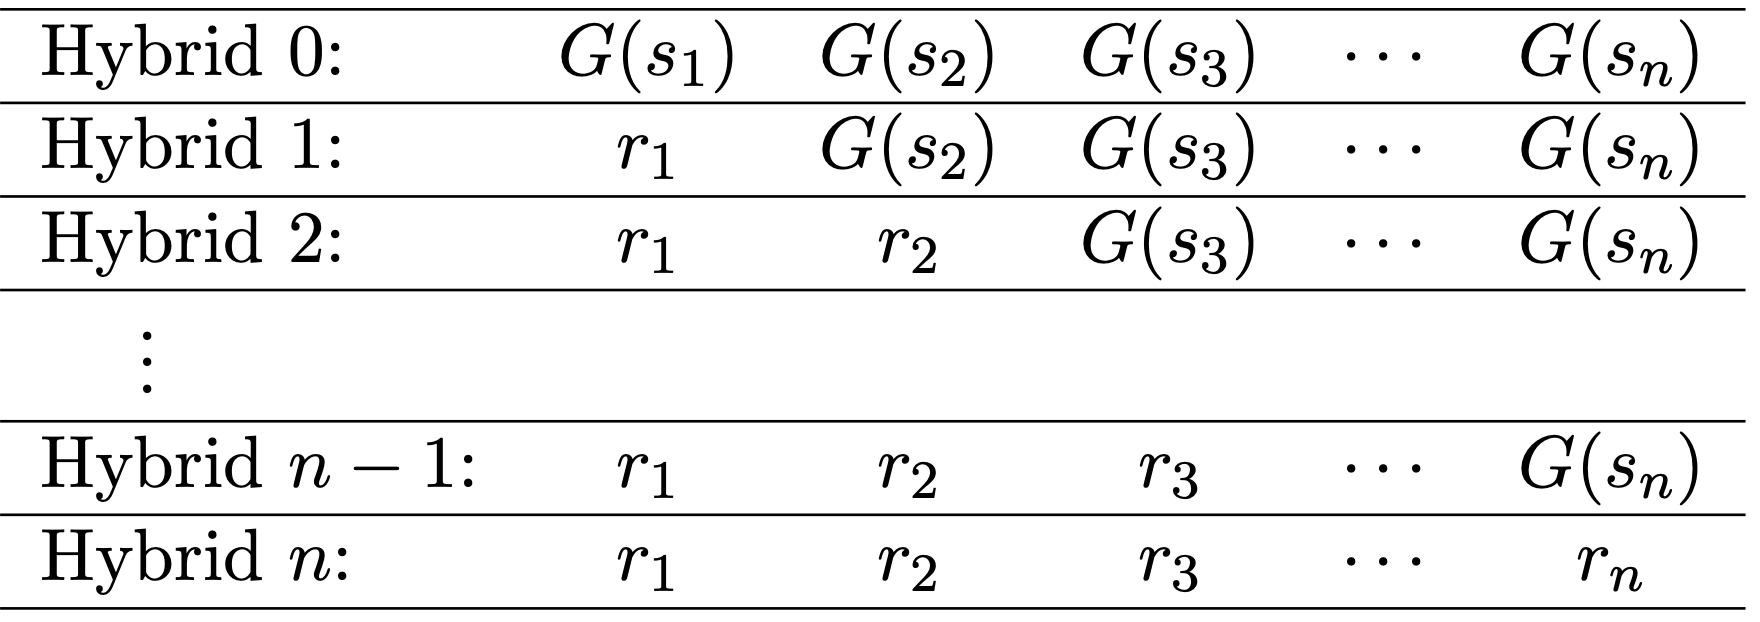
\includegraphics[width=0.55\linewidth]{figures/chapter3/fig5.png}
  \caption{挑战者在混合$0,1,\dots,n$中准备的数值。每个$r_i$都是$\mathcal{R}$上的一个随机元素,每个$s_i$都是$\mathcal{S}$上的一个随机元素。}
  \label{fig:3-5}
\end{figure}

接下来我们定义一个 PRG 对手 $\mathcal B$,它对 $G$ 进行攻击游戏 \ref{game:3-1} 中的攻击,其工作方式如下:

\vspace*{5pt}

\hspace*{5pt} 当收到来自挑战者的 $r\in\mathcal R$,$\mathcal B$ 扮演 $\mathcal A$ 的挑战者的角色:\\
\hspace*{50pt} $\omega\overset{\rm R}\leftarrow\{1,\dots,n\}$\\
\hspace*{50pt} $r_1\overset{\rm R}\leftarrow\mathcal R$\\
\hspace*{74pt} $\vdots$\\
\hspace*{50pt} $r_{\omega-1}\overset{\rm R}\leftarrow\mathcal R$\\
\hspace*{50pt} $r_{\omega}\leftarrow r$\\
\hspace*{50pt} $s_{\omega+1}\overset{\rm R}\leftarrow\mathcal{S},\;r_{\omega+1}\leftarrow G(s_{\omega+1})$\\
\hspace*{74pt} $\vdots$\\
\hspace*{50pt} $s_{n}\overset{\rm R}\leftarrow\mathcal{S},\;r_{n}\leftarrow G(s_{j+1})$\\
\hspace*{50pt} 将 $(r_1,\dots,r_n)$ 发送给 $\mathcal A$。\\
\hspace*{26pt} 最后,$\mathcal B$ 输出 $\mathcal A$ 所输出的任何东西。

\vspace*{5pt}

令 $W_0$ 是$\mathcal B$ 在攻击游戏 \ref{game:3-1} 的实验 $0$ 中输出 $1$ 的事件,$W_1$ 是$\mathcal B$在攻击游戏 \ref{game:3-1} 的实验 $1$ 中输出 $1$ 的事件。一个关键的观察是:

\begin{quote}
\emph{对于每个固定的 $j=1,\dots,n$,以 $\omega=j$ 为条件,$\mathcal B$ 的攻击游戏的实验 $0$ 就相当于混合 $j-1$,而 $\mathcal B$ 的攻击游戏的实验 $1$ 则相当于混合 $j$。
}
\end{quote}
因此:
$$
\Pr[W_0\,|\,\omega=j]=p_{j-1},\quad
\Pr[W_1\,|\,\omega=j]=p_{j}
$$
所以,我们有:
$$
\Pr[W_0]
=\sum_{j=1}^n\Pr[W_0\,|\,\omega=j]\Pr[\omega=j]
=\frac{1}{n}\sum_{j=1}^n\Pr[W_0\,|\,\omega=j]
=\frac{1}{n}\sum_{j=1}^np_{j-1}
$$
类似地:
$$
\Pr[W_1]
=\sum_{j=1}^n\Pr[W_1\,|\,\omega=j]\Pr[\omega=j]
=\frac{1}{n}\sum_{j=1}^n\Pr[W_1\,|\,\omega=j]
=\frac{1}{n}\sum_{j=1}^np_{j}
$$
最终,我们有:
$$
\begin{aligned}
{\rm PRG\mathsf{adv}}[\mathcal{B},G]
&=|\Pr[W_1]-\Pr[W_0]|\\
&=\Bigg\lvert\frac{1}{n}\sum_{j=1}^np_j-\frac{1}{n}\sum_{j=1}^np_{j-1}\Bigg\rvert\\
&=\frac{1}{n}|p_n-p_0|
\end{aligned}
$$
将其与式 \ref{eq:3-9} 相结合,我们可以得到:
$$
{\rm PRG\mathsf{adv}}[\mathcal{A},G']=n\cdot{\rm PRG\mathsf{adv}}[\mathcal{B},G]
$$
由于我们假设 $G$ 是一个安全 PRG,因此 ${\rm PRG\mathsf{adv}}[\mathcal{B},G]$ 可以忽略不计,而由于 $n$ 是多项式边界的,${\rm PRG\mathsf{adv}}[\mathcal{B},G']$ 也是可忽略不计的(见事实 \ref{fact:2-6})。这就证明了该定理。
\end{proof}

定理 3.2 表明,PRG 的安全性随着我们使用它的次数增多而最多呈线性下降。有人可能会问,这个约束是否是严格的?也即,安全性是否真的会随着使用次数的增加而线性下降?答案其实是肯定的(见练习 3.14)。

\subsection{一种串行构造:Blum-Micali 方法}\label{subsec:3-4-2}

我们下面介绍一种由 Blum 和 Micali 发明的串行构造,它使用一个只稍做延展的 PRG,建立一个可以伸展到任意长度的 PRG。

令 $G$ 是一个定义在 $(\mathcal{S},\mathcal{R}\times\mathcal{S})$ 上的 PRG,其中 $\mathcal S$ 和 $\mathcal R$ 是有限集。对于每个多项式边界的值 $n\geq 1$,我们可以构造一个定义在 $(\mathcal{S},\mathcal{R}^n\times\mathcal{S})$ 上的新的 PRG $G'$。对于 $s\in\mathcal{S}$,我们令:

\vspace*{5pt}

\hspace*{5pt} $G'(s):=$\\
\hspace*{50pt} $s_0\leftarrow s$\\
\hspace*{50pt} 对于 $i\leftarrow1$ 到 $n$:\\
\hspace*{75pt} $(r_i,s_i)\leftarrow G(s_{i-1})$\\
\hspace*{50pt} 输出$(r_1,\dots,r_n,s_n)$

\vspace*{5pt}

\noindent
我们称 $G'$ 为 $G$ 的 \textbf{$n$ 次串行组合 ($n$-wise sequential composition)}。图 \ref{fig:3-6} 是 $n=3$ 时$G'$ 的示意图。

\begin{figure}
  \centering
  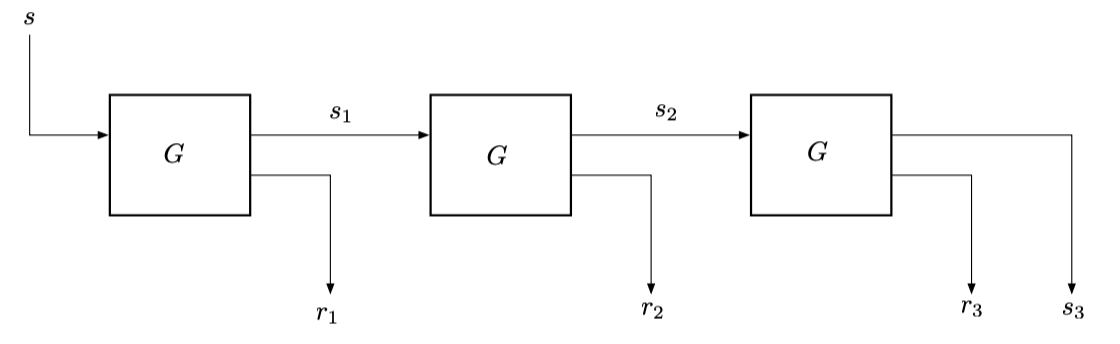
\includegraphics[width=0.8\linewidth]{figures/chapter3/fig6.png}
  \caption{$n=3$时的串行构造}
  \label{fig:3-6}
\end{figure}

我们将在下面的定理 \ref{theo:3-3} 中证明,如果 $G$ 是一个安全 PRG,那么 $G'$ 也是一个安全 PRG。作为这个构造的一个特例,假设 $G$ 是一个定义在 $(\{0,1\}^\ell,\{0,1\}^{t+\ell})$ 上的 PRG,其中 $\ell$ 和 $t$ 是正整数;也就是说,$G$ 把 $\ell$ 比特字符串拉伸为 $t+\ell$ 比特字符串。我们可以很自然地把 $G$ 的输出空间看作是 $\{0,1\}^t\times\{0,1\}^\ell$。应用上述构造,并把输出解释为比特串,我们就能得到一个PRG $G'$,它能把 $\ell$ 位比特串拉伸为 $nt+\ell$ 位比特串。

\begin{theorem}\label{theo:3-3}
如果 $G$ 是一个安全 PRG,那么 $G$ 的 $n$ 次串行组合 $G'$ 也是一个安全 PRG。
\begin{quote}
特别地,对于每个就 $G'$ 进行攻击游戏 \ref{game:3-1} 的 PRG 对手 $\mathcal A$,都存在一个就 $G$ 进行攻击游戏 \ref{game:3-1} 的 PRG 对手 $\mathcal B$,其中 $\mathcal B$ 是围绕 $\mathcal A$ 的一个基本包装器,满足:
\end{quote}
$$
{\rm PRG\mathsf{adv}}[\mathcal{A},G']=n\cdot{\rm PRG\mathsf{adv}}[\mathcal{B},G]
$$
\end{theorem}

\begin{proof}[证明思路]
该定理的证明是一个混合论证,其思路与定理 \ref{theo:3-2} 的证明非常相似。该证明背后的直觉如下所述。考虑一个 PRG 对手 $\mathcal A$,他在攻击游戏 \ref{game:3-1} 的实验 $0$ 中收到 $(r_1,\dots,r_n,s_n)$。由于 $s=s_0$ 是随机的,而且 $G$ 是一个安全 PRG,我们可以用 $\mathcal{R}\times\mathcal{S}$ 中的一个完全随机的元素来代替 $(r_1,s_1)$,且 $\mathcal A$ 在这个新的混合游戏中输出 $1$ 的概率应该只会发生可忽略不计的变化。现在,由于 $s_1$ 是随机的(同样是因为$G$ 是一个安全 PRG),我们就可以用 $\mathcal{R}\times\mathcal{S}$ 上的一个完全随机的元素来代替 $(r_2,s_2)$,而 $\mathcal A$ 在这第二个混合游戏中输出 $1$ 的概率应该也只会发生可忽略不计的变化。继续这样下去,我们可以用 $\mathcal{R}\times\mathcal{S}$ 中的随机元素逐步替换 $(r_3,s_3)$ 到 $(r_n,s_n)$,在做出这些改变之后,$\mathcal A$ 输出 $1$ 的概率应该都只会发生可忽略不计的变化(假设$n$是多项式边界的)。然而,在这一点上,$\mathcal A$ 输出 $1$ 的概率与他在攻击游戏 \ref{game:3-1} 的实验 $1$ 中输出 $1$ 的概率相同,因此,这个概率与$\mathcal A$在攻击游戏 \ref{game:3-1} 的实验 $0$ 中输出 $1$ 的概率接近得可以忽略不计。

这就是我们的想法;然而,就像在定理 \ref{theo:3-2} 的证明中一样,由于技术原因,我们设计了一个攻击$G$的 PRG 对手。
\end{proof}

\begin{proof}
令 $\mathcal A$ 是一个对 $G'$ 进行攻击游戏 \ref{game:3-1} 中的攻击的 PRG 对手。我们首先引入一个大小为 $n+1$ 的混合游戏序列,称为混合$0$,混合$1$,$\dots$,混合$n$。对于$j=0,1,\dots,n$,我们定义混合 $j$ 为 $\mathcal A$ 和以下挑战者之间的游戏。挑战者的工作方式如下:

\vspace*{5pt}

\hspace*{5pt} $r_1\overset{\rm R}\leftarrow\mathcal R$\\
\hspace*{50pt} $\vdots$\\
\hspace*{26pt} $r_j\overset{\rm R}\leftarrow\mathcal R$\\
\hspace*{26pt} $s_j\overset{\rm R}\leftarrow\mathcal S$\\
\hspace*{26pt} $(r_{j+1},s_{j+1})\leftarrow G(s_{j})$\\
\hspace*{50pt} $\vdots$\\
\hspace*{26pt} $(r_n,s_{n})\leftarrow G(s_{n-1})$\\
\hspace*{26pt} 将 $(r_1,\dots,r_n,s_n)$ 发送给 $\mathcal A$。

\vspace*{5pt}

\noindent
像之前一样,$\mathcal A$ 在游戏结束时输出 $0$ 或 $1$。图 \ref{fig:3-7} 展示了挑战者在 $n=3$ 的情况下的工作流程。请注意,$p_0$ 也等于 $\mathcal A$ 在攻击游戏 \ref{game:3-1} 的实验 $0$ 中输出 $1$ 的概率,而 $p_n$ 则等于 $\mathcal A$ 在攻击游戏 \ref{game:3-1} 的实验 $1$ 中输出 $1$ 的概率。因此,我们有:
\begin{equation}
{\rm PRG\mathsf{adv}}[\mathcal{A},G']=|p_n-p_0|
\end{equation}

接下来我们定义一个 PRG 对手 $\mathcal B$,它对 $G$ 进行攻击游戏 \ref{game:3-1} 中的攻击,其工作方式如下:

\vspace*{5pt}

\hspace*{5pt} 当收到来自挑战者的 $(r,s)\in\mathcal{R}\times\mathcal{S}$,$\mathcal B$ 扮演 $\mathcal A$ 的挑战者的角色:\\
\hspace*{50pt} $\omega\overset{\rm R}\leftarrow\{1,\dots,n\}$\\
\hspace*{50pt} $r_1\overset{\rm R}\leftarrow\mathcal R,\dots,r_{\omega-1}\overset{\rm R}\leftarrow\mathcal R$\\
\hspace*{50pt} $(r_{\omega},s_{\omega})\leftarrow(r,s)$\\
\hspace*{50pt} $(r_{\omega+1},s_{\omega+1})\leftarrow G(s_{\omega}),\dots,(r_n,s_n)\leftarrow G(s_{n-1})$\\
\hspace*{50pt} 将 $(r_1,\dots,r_n,s_n)$ 发送给 $\mathcal A$。\\
\hspace*{26pt} 最后,$\mathcal B$ 输出 $\mathcal A$ 所输出的任何东西。

\vspace*{5pt}

令 $W_0$ 是$\mathcal B$在攻击游戏 \ref{game:3-1} 的实验 $0$ 中输出 $1$ 的事件,$W_1$ 是$\mathcal B$在攻击游戏 \ref{game:3-1} 的实验 $1$ 中输出 $1$ 的事件。一个关键的观察是:
\begin{quote}
\emph{对于每个固定的 $j=1,\dots,n$,以 $\omega=j$ 为条件,$\mathcal B$ 的攻击游戏的实验 $0$ 等同于混合 $j-1$,而 $\mathcal B$ 的攻击游戏的实验 $1$ 则等同于混合 $j$。
}
\end{quote}
因此:
$$
\Pr[W_0\,|\,\omega=j]=p_{j-1},\quad
\Pr[W_1\,|\,\omega=j]=p_{j}
$$

\begin{figure}
  \centering
  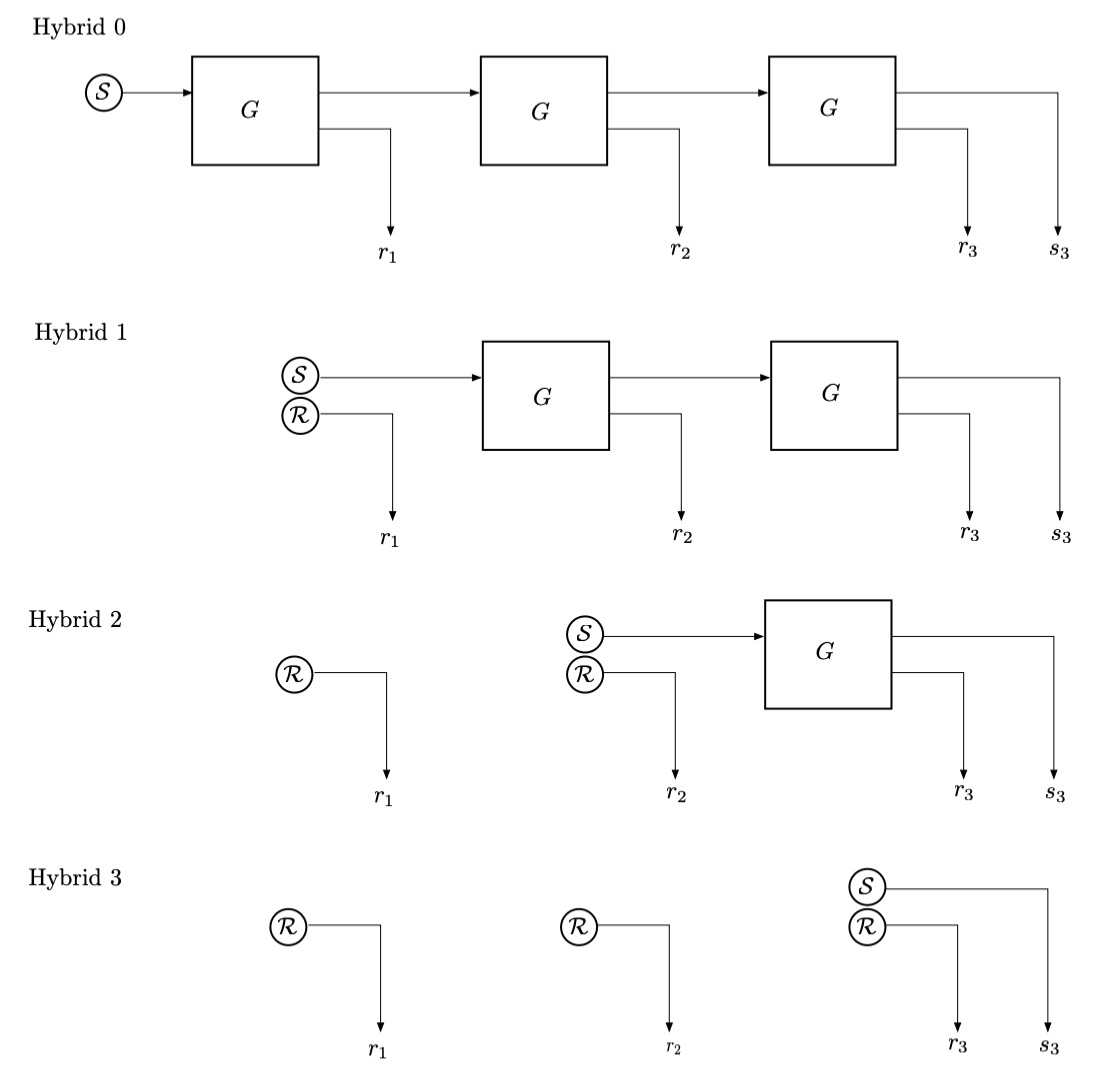
\includegraphics[width=0.8\linewidth]{figures/chapter3/fig7.png}
  \caption{$n=3$时,混合游戏中挑战者的计算。圆圈表示随机产生的$\mathcal{S}$或$\mathcal{R}$上的元素,如标签所示。}
  \label{fig:3-7}
\end{figure}

接下来的证明只是简单的计算,与定理 \ref{theo:3-2} 的证明的最后一段\emph{相同},不再赘述。
\end{proof}

评价 PRG 的一个标准是它的\textbf{扩展率 (expansion rate)}:一个将 $n$ 比特种子扩展到 $m$ 比特输出的 PRG 的扩展率为 ${m}/{n}$。更一般地说,如果种子空间是 $\mathcal{S}$,输出空间是 $\mathcal{\rm R}$,我们将扩展率定义为 ${\log|\mathcal{\rm R}|}/{\log|\mathcal{S}|}$。串行组合构造比并行组合构造提供了更好的扩展率,但是它有一个缺点,那就是它不能被并行化。事实上,存在一种构造可以兼顾两种优点:大的扩展率和高度可并行的结构,见 \ref{subsec:4-4-4} 小节。

\subsection{数学细节}

在定理 \ref{theo:3-2} 和 \ref{theo:3-3} 的证明中,有一些微妙的地方值得讨论。

首先,在这两个构造中,底层的 PRG $G$ 可能有系统参数。也就是说,可能存在一个概率性算法,它将安全参数 $\lambda$ 作为输入,并输出一个系统参数 $\Lambda$。回顾一下,系统参数是能够完全将构造实例化的公共数据(在这个场景中,它可能定义了种子空间和输出空间)。对于并行和串行构造,我们可以对 $G$ 的所有 $n$ 个实例使用相同的系统参数;事实上,对于串行构造来说,这是必须的,因为我们要确保一轮的输出可以被用作下一轮的输入。无论是对所有 $G$ 的实例使用相同的系统参数,还是对不同的实例使用不同的系统参数,这些安全定理的证明都是完全有效的。

其次,我们要简要讨论关于混合论证的一个相当深奥的问题。为了更具体一点,我们把注意力集中在定理 \ref{theo:3-2} 的证明上(尽管类似的讨论也适用于定理 \ref{theo:3-3} 的证明,或任何其他的混合论证)。在证明该定理时,我们最终想要证明,如果存在一个能破解 $G'$ 的有效对手 $\mathcal A$,那么也必然存在一个能破解 $G$ 的有效对手。假设 $\mathcal A$ 是一个能破解 $G'$ 的有效对手,那么它相对于 $G'$ 的优势 $\epsilon(\lambda)$(我们这里明确地把它表示成安全参数$\lambda$的一个函数)是不可忽略不计的。这意味着存在一个常数 $c$使得 $\epsilon(\lambda)\geq{1}/{\lambda^c}$适用于无限多的 $\lambda$。

现在,在定理 \ref{theo:3-2} 证明之前的讨论中,我们考虑了 $n=2$ 的特殊情况,并表明存在有效对手 $\mathcal{B}_1$ 和 $\mathcal{B}_2$,使得 $\epsilon(\lambda)\leq\delta_1(\lambda)+\delta_2(\lambda)$ 对于任意 $\lambda$ 都成立,其中 $\delta_j(\lambda)$ 表示 $\mathcal{B}_j$ 相对于 $G$ 的优势。由此可见,要么 $\delta_1(\lambda)\geq{1}/{2\lambda^c}$ 无限频繁,要么 $\delta_2(\lambda)\geq{1}/{2\lambda^c}$ 无限频繁。因此我们可以得出结论,要么是$\mathcal{B}_1$ 打破 $G$,要么是$\mathcal{B}_2$ 打破 $G$(也可能两者皆然)。因此,\emph{存在}一个能破解 $G$ 的有效对手:它要么是 $\mathcal{B}_1$ 要么是 $\mathcal{B}_2$,我们不知道到底是哪一个(也不必分清是哪一个)。然而无论是哪一个,它都是一个固定的对手,对所有的 $\lambda$ 都是统一定义的;也就是说,它是一个固定的,以 $\lambda$ 为输入的机器。

这个论证是完全有效的,并且可以扩展到任意\emph{常数} $n$:我们可以构造 $n$ 个对手 $\mathcal{B}_1,\dots,\mathcal{B}_n$,并论证对于某个 $j\in\{1,\dots,n\}$,对手 $\mathcal{B}_j$ 无限频繁地对 $G$ 有优势 ${1}/{n\lambda^c}$,从而攻破 $G$。然而这个论证并没有扩展到 $n$ 是 $\lambda$ 的函数的情况,我们现在把它明确写成 $n(\lambda)$。问题不在于 ${1}/({n(\lambda)\lambda^c})$ 也许太小(其实并不是)。这个问题相当微妙,所以在我们讨论它之前,让我们先回顾一下我们所给出的(合法)证明。对于每个 $\lambda$,我们定义一个大小为 $n(\lambda)+1$ 的混合游戏序列,因此对于每个 $\lambda$,我们实际上得到了一个不同的游戏序列。事实上,我们不能说有一个单一、有限的游戏序列对所有 $\lambda$ 都有效,因为 $n(\lambda)\to\infty$。尽管如此,我们还是明确地构造了一个固定的对手 $\mathcal B$,它是为所有 $\lambda$ 统一定义的;也就是说,$\mathcal B$ 是一个固定的机器,它把 $\lambda$ 作为输入。我们为每个 $\lambda$ 定义的混合游戏序列是一个数学对象,我们对其可计算性不做任何主张,它只是在分析 $\mathcal B$ 时使用的一个方便的工具。

希望到现在为止,读者至少对我们试图将常数 $n$ 的论证推广到一个函数 $n(\lambda)$ 时所产生的问题有了一个直观感觉。首先,我们甚至不清楚 $n(\lambda)$ 个对手 $\mathcal{B}_1,\dots,\mathcal{B}_{n(\lambda)}$ 是什么意思:我们的对手应该是将 $\lambda$ 作为输入的固定机器,而机器本身不应该依赖于 $\lambda$。撇开这种语言上的混乱不谈,我们对常数情况的证明只表明存在一个``对手",对于无限多的 $\lambda$ 值来说,它能以某种方式知道 $j=j(\lambda)$ 的``正确"值,以便在 $(n(\lambda)+1)$ 游戏混合论证中使用——没有一个 $j$ 常数值一定对无限多的 $\lambda$ 有效。如果使用非统一的计算模型,我们实际上可以使这种类型的论证有意义,但我们在本文中不会采取这种方法。

当我们使用一个构建单一对手 $\mathcal B$ 的混合论证时,所有这些问题都会消失,就像我们在定理 \ref{theo:3-2} 和 \ref{theo:3-3} 的证明中所做的。然而我们重申,我们在 $n=2$,或自然延伸到每一个常数 $n$ 的情况下所做的原始分析是完全有效的。在这种情况下,我们构建了一个单一、固定的 $n+1$ 游戏序列,每个单独的游戏对所有 $\lambda$ 都是统一定义的(就像我们的安全定义中的攻击游戏一样),我们还定义了一个有限的对手集合,每个对手都是一个固定的机器。我们重申这一点,因为在后面的内容中,我们将经常构建涉及这样的有限序列游戏的证明(事实上,定理\ref{theo:3-1}的证明就是这种类型)。在这种情况下,每个游戏将为所有 $\lambda$ 统一定义,并被称为游戏 $0$、游戏 $1$,等等。相反,当我们进行混合论证,使用非均匀的游戏序列时,我们将这些游戏表示为混合 $0$,混合 $1$ 等,以避免任何可能的混淆。
\section{下一比特测试}

令 $G$ 是一个定义在 $(\{0,1\}^\ell,\{0,1\}^L)$ 上的 PRG,它能将 $\ell$ 比特字符串拉伸到 $L$ 比特长。有许多方法可以让对手区分 $G$ 的伪随机输出和真正的随机比特序列。事实上,假设一个有效对手能在给定 $G$ 输出的前 $L-1$ 比特的情况下预测出其输出的最后一比特,则 $G$ 从直观上来说就是不安全的,因为给定一个真随机 $L$ 位比特序列的前 $L-1$ 位,任何人最多只有一半的机会猜中最后一比特。事实上,该结论一个有趣的逆命题也是真命题。

我们下面会正式定义 PRG 的\textbf{不可预测性 (unpredictability)} 的概念。它本质上指,给定 $G$ 输出的前 $i$ 比特(这里的$i$是一个对手选择的索引),能够以显著高于$1/2$的概率预测出下一个比特(即第 $i+1$ 比特)是困难的。之后,我们将证明不可预测性和安全性是等价的。安全性能够导出不可预测性这一事实是很直观的:如果能够有效预测伪随机序列中的下一比特,那么我们就能直接给出一个有效的统计测试来打破安全性。相反,由不可预测性能够导出安全性,这是相当有趣的(需要花一些精力来证明),这实际上是指,如果存在任何有效的统计测试能够打破 PRG 的安全性,那么必然存在一个方法能够有效预测伪随机序列将要输出的下一比特。

\begin{game}[不可预测的 PRG]\label{game:3-2}
对于一个定义在 $(\mathcal{S},\{0,1\}^L)$ 上的给定 PRG $G$ 和一个给定对手 $\mathcal{A}$,攻击游戏的过程如下:
\begin{itemize}
	\item 对手向挑战者发送一个索引 $i$,其中 $0\leq i\leq L-1$。
	\item 挑战者计算
	$$s\overset{\rm R}\leftarrow\mathcal{S},\;\; r\leftarrow G(s)$$
	并将 $r[0\dots i-1]$ 发送给对手。
	\item 对手输出 $g\in\{0,1\}$。
\end{itemize}
如果 $r[i]=g$,我们就说 $\mathcal{A}$ \textbf{获胜}。我们定义 $\mathcal{A}$ 相对于 $G$ 的\textbf{优势}为 ${\rm Pred\mathsf{adv}}[\mathcal{A},G]$,其值为$|\Pr[\mathcal{A}\text{ wins}]-{1}/{2}|$。
\end{game}

\begin{definition}[不可预测的 PRG]
如果 ${\rm Pred\mathsf{adv}}[\mathcal{A},G]$ 对所有有效对手 $\mathcal{A}$ 来说都是可忽略不计的,那么 PRG $G$ 就是\textbf{不可预测的 (unpredictable)}。
\end{definition}

我们下面先证明安全性能够推出不可预测性。

\begin{theorem}
令 $G$ 是一个定义在 $(\mathcal{S},\{0,1\}^L)$ 上的 PRG。如果 $G$ 是安全的,那么 $G$ 就是不可预测的。
\begin{quote}
特别地,对于每个如攻击游戏 \ref{game:3-2} 那样攻击 $G$ 的不可预测性对手 $\mathcal{A}$,必然存在一个如攻击游戏 \ref{game:3-1} 那样攻击 $G$ 的安全性对手 $\mathcal{B}$,其中 $\mathcal{B}$ 是围绕 $\mathcal{A}$ 的一个基本包装器,满足:
\end{quote}
$$
{\rm Pred\mathsf{adv}}[\mathcal{A},G]={\rm PRG\mathsf{adv}}[\mathcal{B},G]
$$
\end{theorem}

\begin{proof}
令 $\mathcal{A}$ 是一个攻击 $G$ 的不可预测性的对手,令 $i$ 表示 $\mathcal{A}$ 所选择的索引。同时,假设 $\mathcal{A}$ 能以 ${1}/{2}+\epsilon$ 的概率赢得攻击游戏 \ref{game:3-2},则有${\rm Pred\mathsf{adv}}[\mathcal{A},G]=|\epsilon|$。

我们下面以 $\mathcal{A}$ 为子程序,建立一个攻击 $G$ 的安全性的对手 $\mathcal{B}$,其运行方式如下:

\vspace*{5pt}

\hspace*{5pt} 当收到来自挑战者的 $r\in\{0,1\}^L$ 时,$\mathcal B$ 进行以下操作:\\
\hspace*{50pt} $\mathcal{B}$ 将 $r[0\dots i-1]$ 发送 $\mathcal{A}$,获得 $\mathcal{A}$ 的输出 $g\in\{0,1\}$;\\
\hspace*{50pt} 如果 $r[i]=g$,$\mathcal{B}$ 输出 $1$,否则输出 $0$。

\vspace*{5pt}

对于 $b=0,1$,令 $W_b$ 为$\mathcal{B}$在攻击游戏 \ref{game:3-1} 的实验 $b$ 中输出 $1$ 的事件。在实验 $0$ 中,$r$ 是 $G$ 的一个伪随机输出,当且仅当 $r[i]=g$ 时 $W_0$ 才会发生,因此根据定义,有:
$$
\Pr[W_0]={1}/{2}+\epsilon
$$
在实验 $1$ 中,$r$ 是一个真随机比特序列。同样地,当且仅当 $r[i]=g$ 时 $W_1$ 才会发生;然而,在这种情况下,随机变量 $r[i]$ 和 $g$ 的值相互独立,因此有:
$$
\Pr[W_1]={1}/{2}
$$
因此可以得到:
$$
{\rm Pred\mathsf{adv}}[\mathcal{B},G]=|\Pr[W_1]-\Pr[W_0]|=|\epsilon|={\rm PRG\mathsf{adv}}[\mathcal{A},G]
$$
\end{proof}

更有趣也更有挑战性的任务是证明不可预测性能够推出着安全性。在详细介绍具体的证明之前,我们先勾勒出高层次的想法。

首先,我们会采用一个混合论证,目的是论证如果 $\mathcal{A}$ 是一个能够有效区分伪随机 $L$ 比特序列和真随机 $L$ 比特序列的有效对手,那么我们必然可以构造一个有效对手 $\mathcal{B}$,他能够有效地区分:
$$
x_1\cdots x_j~r
$$
和:
$$
x_1\cdots x_j~x_{j+1}
$$
其中 $j$ 是一个随机选出的索引,$x_1,\dots,x_L$ 是伪随机输出,而 $r$ 是一个随机比特。因此,对手 $\mathcal{B}$ 可以在给定 $x_1,\dots,x_j$ 这个``侧信息"的情况下有效区分伪随机比特 $x_{j+1}$ 和真随机比特 $r$。

我们想把 $\mathcal{B}$ 的区分优势变成预测优势,大致的想法是这样的:给定 $x_1,\dots,x_j$,我们给 $\mathcal{B}$ 提供一个序列 $x_1\cdots x_j~r$,其中的 $r$ 是一个随机选出的比特;如果 $\mathcal{B}$ 输出 $1$,我们对 $x_{j+1}$ 的预测值就是 $r$;否则我们对 $x_{j+1}$ 的预测值就是 $\overline r$($r$ 的补码)。

这一预测策略的有效性由以下的一般结论给出,我们称之为\emph{区分者/预测者引理}。我们有一半设置如下:
\begin{itemize}
	\item 一个随机变量 $\mathsf{X}$,它对应于上面的``侧信息" $x_1,\dots,x_j$ 以及对手 $\mathcal{B}$ 所使用的任何随机硬币;
	\item 一个取值为 $0$ 或 $1$ 的随机变量 $\mathsf{B}$,它对应于上面的 $x_{j+1}$,并可能与 $\mathsf{X}$ 相关;
	\item 一个取值为 $0$ 或 $1$ 的随机变量 $\mathsf{R}$,它对应于上面的 $r$,并且与 $(\mathsf{X},\mathsf{B})$ 无关。
	\item 一个函数 $d$,它对应于使得$\mathcal{B}$的区分优势为$|\epsilon|$的策略,其中$\epsilon=\Pr[d(\mathsf{X},\mathsf{B})=1]-\Pr[d(\mathsf{X},\mathsf{R})=1]$。
\end{itemize}
该引理表明,如果我们用上述预测策略定义 $\mathsf{B}'$,即如果 $d(\mathsf{X},\mathsf{R})=1$,就有 $\mathsf{B}'=\mathsf{R}$,否则有 $\mathsf{B}'=\mathsf{\overline R}$,那么预测 $\mathsf{B}'$ 等于实际值 $\mathsf{B}$ 的概率正好是 ${1}/{2}+\epsilon$。下面是该引理的精确陈述:

\begin{lemma}[区分者/预测者引理]\label{lemma:3-5}
令 $\mathsf{X}$ 是一个在某个集合 $S$ 中取值的随机变量,令 $\mathsf{B}$ 和 $\mathsf{R}$ 是取值为 $0$ 或 $1$ 的随机变量,其中 $\mathsf{R}$ 在 $\{0,1\}$ 上均匀分布,且与 $(\mathsf{X},\mathsf{B})$ 无关。令 $d:S\times\{0,1\}\to\{0,1\}$ 是一个任意的函数,并令:
$$
\epsilon:=\Pr[d(\mathsf{X},\mathsf{B})=1]-\Pr[d(\mathsf{X},\mathsf{R})=1]
$$
随机变量 $\mathsf{B}'$的定义如下:
$$
\mathsf{B}':=
\left\{
\begin{array}{ll}
\mathsf{R}, & d(\mathsf{X},\mathsf{R})=1\\
\mathsf{\overline R}, & d(\mathsf{X},\mathsf{R})\neq 1
\end{array}
\right.
$$
则有:
$$
\Pr[\mathsf{B}'=\mathsf{B}]={1}/{2}+\epsilon
$$
\end{lemma}

\begin{proof}
我们首先以事件 $\mathsf{B}=\mathsf{R}$ 和 $\mathsf{B}=\mathsf{\overline R}$ 为条件计算 $\Pr[\mathsf{B}'=\mathsf{B}]$:

$$
\begin{aligned}
\Pr[\mathsf{B}'=\mathsf{B}]
&=\Pr[\mathsf{B}'=\mathsf{B}\,|\,\mathsf{B}=\mathsf{R}]\cdot\Pr[\mathsf{B}=\mathsf{R}]+\Pr[\mathsf{B}'=\mathsf{B}\,|\,\mathsf{B}=\mathsf{\overline R}]\cdot\Pr[\mathsf{B}=\mathsf{\overline R}]\\
&=\Pr[d(\mathsf{X},\mathsf{R})=1\,|\,\mathsf{B}=\mathsf{R}]\cdot\frac{1}{2}+\Pr[d(\mathsf{X},\mathsf{R})=0\,|\,\mathsf{B}=\mathsf{\overline R}]\cdot\frac{1}{2}\\
&=\frac{1}{2}
\Big(\Pr[d(\mathsf{X},\mathsf{R})=1\,|\,\mathsf{B}=\mathsf{R}]+
\big(
1-\Pr[d(\mathsf{X},\mathsf{R})=1\,|\,\mathsf{B}=\mathsf{\overline R}]
\big)
\Big)\\
&=\frac{1}{2}+\frac{1}{2}(\alpha-\beta)
\end{aligned}
$$
其中:
$$
\alpha:=\Pr[d(\mathsf{X},\mathsf{R})=1\,|\,\mathsf{B}=\mathsf{R}],\quad
\beta:=\Pr[d(\mathsf{X},\mathsf{R})=1\,|\,\mathsf{B}=\mathsf{\overline R}]
$$
根据独立性,我们有:
$$
\alpha=\Pr[d(\mathsf{X},\mathsf{R})=1\,|\,\mathsf{B}=\mathsf{R}]=\Pr[d(\mathsf{X},\mathsf{B})=1\,|\,\mathsf{B}=\mathsf{R}]=\Pr[d(\mathsf{X},\mathsf{B})=1]
$$
想要知道最后一个等式为什么成立,可以参考练习 3.25 的结论。

因此,我们可以计算出:
$$
\begin{aligned}
\epsilon
&=\Pr[d(\mathsf{X},\mathsf{B})=1]-\Pr[d(\mathsf{X},\mathsf{R})=1]\\
&=\alpha-
\Big(\Pr[d(\mathsf{X},\mathsf{R})=1\,|\,\mathsf{B}=\mathsf{R}]\cdot\Pr[\mathsf{B}=\mathsf{R}]+\Pr[d(\mathsf{X},\mathsf{R})=1\,|\,\mathsf{B}=\mathsf{\overline R}]\cdot\Pr[\mathsf{B}=\mathsf{\overline R}]
\Big)\\
&=\alpha-\frac{1}{2}(\alpha+\beta)\\
&=\frac{1}{2}(\alpha-\beta)
\end{aligned}
$$
这就证明了该引理。
\end{proof}

\begin{theorem}
令 $G$ 是一个定义在 $(\mathcal{S},\{0,1\}^L)$ 上的 PRG。如果 $G$ 是不可预测的,那么 $G$ 就是安全的。
\begin{quote}
特别地,对于每个像攻击游戏 \ref{game:3-1} 那样攻击 $G$ 的安全性的对手 $\mathcal{A}$,必然存在一个像攻击游戏 \ref{game:3-2} 那样攻击 $G$ 的不可预测性的对手 $\mathcal{B}$,其中 $\mathcal{B}$ 是围绕 $\mathcal{A}$ 的一个基本包装器,满足:
\end{quote}
$$
{\rm PRG\mathsf{adv}}[\mathcal{A},G]=L\cdot{\rm Pred\mathsf{adv}}[\mathcal{B},G]
$$
\end{theorem}

\begin{proof}
令 $\mathcal{A}$ 像攻击游戏 \ref{game:3-1} 中那样攻击 $G$。利用 $\mathcal{A}$,我们建立一个预测器 $\mathcal{B}$,它像攻击游戏 \ref{game:3-2} 那样攻击 $G$。$\mathcal{B}$ 的工作方式如下:
\begin{itemize}
	\item 随机选出 $\omega\in\{1,\dots,L\}$。
	\item 向挑战者发送 $L-\omega$,得到一个字符串 $x\in\{0,1\}^{L-\omega}$。
	\item 随机生成 $\omega$ 个比特 $r_1,\dots,r_\omega$,并将 $L$ 比特序列 $x~||~r_1\cdots r_\omega$ 发送给 $\mathcal{A}$。
	\item 如果 $\mathcal{A}$ 输出 $1$,则 $\mathcal{B}$ 输出 $r_1$,否则 $\mathcal{B}$ 输出 $\overline r_1$。
\end{itemize}

为了分析 $\mathcal{B}$,我们考虑 $L+1$ 个混合游戏,称为混合$0$,混合$1$,$\dots$,混合$L$。对于 $j=0,\dots,L$,我们定义混合 $j$ 为 $\mathcal{A}$ 和挑战者之间的游戏,挑战者生成一个由 $L-j$ 个伪随机比特和 $j$ 个真随机比特组成的序列 $r$;也就是说,挑战者随机选择 $s\in\mathcal{S}$ 和 $t\in\{0,1\}^j$,并向 $\mathcal{A}$ 发送比特序列:
$$
r=G(s)[0\dots L-j-1]~||~t
$$
和之前一样,$\mathcal{A}$ 在游戏结束时输出 $0$ 或 $1$,我们定义 $p_j$ 为 $\mathcal{A}$ 在混合 $j$ 中输出 $1$ 的概率。注意 $p_0$ 是 $\mathcal{A}$ 在攻击游戏 \ref{game:3-1} 的实验 $0$ 中输出 $1$ 的概率,而 $p_L$ 是 $\mathcal{A}$ 在攻击游戏 \ref{game:3-1} 的实验 $1$ 中输出 $1$ 的概率。

令 $W$ 为 $\mathcal{B}$ 在攻击游戏 \ref{game:3-2} 中获胜的事件(即他正确预测了下一个比特),那么我们有:
$$
\begin{aligned}
\Pr[W]
&=\sum_{j=1}^L\Pr[W|\omega=j]\cdot\Pr[\omega=j]\\
&=\frac{1}{L}\sum_{j=1}^L\Pr[W\,|\,\omega=j]\\
&=\frac{1}{L}\sum_{j=1}^L
\Big(\frac{1}{2}+p_{j-1}-p_j
\Big)
\quad\text{\emph{(根据引理} \ref{lemma:3-5}\emph{\,)}}\\
&=\frac{1}{2}+\frac{1}{L}(p_0-p_L)
\end{aligned}
$$
这就证明了该定理。
\end{proof}
\section{案例研究:Salsa 和 ChaCha PRG}\label{sec:3-6}

在实践中,有许多建立 PRG 和流密码的方法。一种方法是使用 \ref{subsec:3-4-2} 小节中介绍的 Blum-Micali 范式来构建 PRG。我们还将会在第\ref{chap:5}章中讨论另一种方法,它将使用一种更加通用的密码学原语(即计数器模式下的\emph{伪随机函数})来构建它们。我们从一个基于后者的构造开始。

Salsa20/12 和 Salsa20/20 是 Dan Bernstein 于 2005 年设计的快速流密码。Salsa20/12 是被选入 eStream 流密码组合的四种Profile 1 流密码之一。eStream 是一个旨在选择适用于实际场景中的快速且安全的流密码的项目。Bernstein 又于 2008 年提出了 Salsa20/12 和 Salsa20/20 的变体,分别被称作 ChaCha12 和 ChaCha20。这些流密码已经被用在了一些广泛部署的协议——比如 TLS 和 SSH——之中了。

\begin{figure}
	\centering
	\input{figures/chapter3/fig8.tex}
	\caption{Salsa 和 ChaCha PRG 的示意图}
	\label{fig:3-8}
\end{figure}

让我们先简单介绍一下 Salsa 和 ChaCha 流密码家族的底层 PRG。这些 PRG 将一个 $256$ 比特的种子和一个 $64$ 比特的 nonce 作为输入。我们暂时先忽略 nonce,简单地将其置为 $0$,我们将在本节末尾讨论 nonce 的作用。Salsa 和 ChaCha PRG 都遵循图 \ref{fig:3-8} 所示的上层结构。它们都包含两个组件:
\begin{itemize}
	\item 一个填充函数 $\mathrm{pad}(s,j,0)$,它将一个 $256$ 比特的种子 $s$ 和一个 $64$ 比特的计数器 $j$ 结合,以生成一个 $512$ 比特的分组。第三个输入是一个 $64$ 比特的 nonce,我们目前先把它置为 $0$。
	\item 一个固定且公开的置换 $\pi:\{0,1\}^{512}\to\{0,1\}^{512}$。
\end{itemize}
这两个组件使用以下算法(见图 \ref{fig:3-8})输出 $L<2^{64}$ 个伪随机分组,每个 $512$ 比特长:

\vspace*{10pt}

\hspace*{5pt} 输入:种子$s\in\{0,1\}^{256}$

\vspace*{5pt}

\hspace*{5pt} 1. \quad 对于 $j\leftarrow0$ 到 $L-1$:\\
\hspace*{26pt} 2. \quad\quad\quad\quad$h_j\leftarrow\mathrm{pad}(s,j,0)\in\{0,1\}^{512}$\\
\hspace*{26pt} 3. \quad\quad\quad\quad$r_j\leftarrow\pi(h_j)\oplus h_j$\\
\hspace*{26pt} 4. \quad 输出 $(r_0,\dots,r_{L-1})$。

\vspace*{10pt}

\noindent
PRG 的最终输出有 $512\cdot L$ 比特长。我们注意到,在 Salsa 和 ChaCha 中,第 $3$ 行中的异或运算实际上是一个更加复杂的操作:将 $512$ 比特的操作数 $h_j$ 和 $\pi(h_j)$ 拆分成 $16$ 个字,每个字长 $32$ 比特,然后逐字计算模 $2^{32}$ 加法。

Salsa 和 ChaCha 的设计是高度并行的,并且可以同时利用多个处理器核心来加快加密速度。此外,它还可以实现对输出分组的随机访问:不必计算出所有的前序分组,就可以单独计算输出中编号为 $j$ 的分组。基于 Blum-Micali 范式的生成器就不具备这些特性。

我们将在下一章的练习 \ref{exer:4-23} 中分析 Salsa 和 ChaCha 的安全性,但在那之前,我们还需要其他的一些密码学工具。

\begin{snote}[实现细节。]
我们下面简单介绍 ChaCha20 中使用的填充函数 $\mathrm{pad}(s,j,n)$ 和置换 $\pi$。填充函数的输入是一个 $256$ 比特的种子$s_0,\dots,s_7\in\{0,1\}^{32}$,一个 $64$ 比特的计数器 $j_0,j_1\in\{0,1\}^{32}$,以及一个 $64$ 比特的 nonce $n_0,n_1\in\{0,1\}^{32}$。它输出一个 $512$ 比特的分组,记为 $x_0,\dots,x_{15}\in\{0,1\}^{32}$。输出会被组织为一个由 $32$ 比特字构成的 $4\times4$ 矩阵,如下所示:
\begin{equation}
\begin{pmatrix}
x_0 & x_1 & x_2 & x_3 \\
x_4 & x_5 & x_6 & x_7 \\
x_8 & x_9 & x_{10} & x_{11} \\
x_{12} & x_{13} & x_{14} & x_{15}
\end{pmatrix}
\longleftarrow
\begin{pmatrix}
c_0 & c_1 & c_2 & c_3 \\
s_0 & s_1 & s_2 & s_3 \\
s_4 & s_5 & s_6 & s_7 \\
j_0 & j_1 & n_0 & n_1
\end{pmatrix}
\end{equation}
其中 $c_0,c_1,c_2,c_3$ 都是固定的 $32$ 比特常数。

通过对一个简单的置换进行固定次数的迭代,我们就能够得到置换 $\pi:\{0,1\}^{512}\to\{0,1\}^{512}$。$\pi$ 的 $512$ 比特输入会被当作一个由 $16$ 个 $32$ 比特字 $x_0,\dots,x_{15}$ 构成的 $4\times4$ 数组。在 ChaCha20 中,函数 $\pi$ 是通过重复 $10$ 次下列步骤实现的:
\begin{center}
\begin{tabular}{ll}
 (1) $\mathrm{QuarterRound}(x_0,x_4,x_8,x_{12})$, & (2) $\mathrm{QuarterRound}(x_1,x_5,x_9,x_{13})$,\\ 
 (3) $\mathrm{QuarterRound}(x_2,x_6,x_{10},x_{14})$, & (4) $\mathrm{QuarterRound}(x_3,x_7,x_{11},x_{15})$,\\  
 (5) $\mathrm{QuarterRound}(x_0,x_5,x_{10},x_{15})$, & (6) $\mathrm{QuarterRound}(x_1,x_6,x_{11},x_{12})$,\\
 (7) $\mathrm{QuarterRound}(x_2,x_7,x_8,x_{13})$, & (8) $\mathrm{QuarterRound}(x_3,x_4,x_9,x_{14})$\\
\end{tabular}
\end{center}
这里,$\mathrm{QuarterRound}(\texttt{a},\texttt{b},\texttt{c},\texttt{d})$ 的定义可参见下面用 C 程序表示的步骤:
\begin{center}
\begin{tabular}{lll}
\texttt{a += b;} & \texttt{d \^{}=  a;} & \texttt{d <<<= 16;}\\
\texttt{c += d;} & \texttt{b \^{}=  c;} & \texttt{b <<<= 12;}\\
\texttt{a += b;} & \texttt{d \^{}=  a;} & \texttt{d <<<= 8;}\\
\texttt{c += d;} & \texttt{b \^{}=  c;} & \texttt{b <<<= 7;}
\end{tabular}
\end{center}
注意到 QuarterRound 的前四个调用,即步骤 (1-4),从左到右分别被应用到 $4\times4$ 矩阵的四列上。接下来的四次调用,即步骤(5-8),分别被应用到了矩阵的四条对角线上。这样,我们就完成了对 ChaCha20 的描述,只是,我们还需要讨论一下 nonce 的使用。
\end{snote}

\begin{snote}[使用nonce。]
虽然我们到目前为止讨论的 PRG 只把种子作为输入,但在实践中使用的许多 PRG 还需要一个额外的输入,称为\emph{nonce}。也就是说,PRG 是一个函数 $G:\mathcal{S}\times\mathcal{N}\to\mathcal{R}$,其中的 $\mathcal{S}$ 和 $\mathcal{R}$ 和之前一样,而 $\mathcal{N}$ 被称为\emph{nonce 空间}。nonce 能让我们使用单个种子 $s$ 产生多个伪随机输出。也就是说,$G(s,n_0)$ 是一个伪随机输出,而当 $n_1\neq n_0$ 时,$G(s,n_1)$ 就是另一个伪随机输出。nonce 将 PRG 变成了一个更强大的密码学原语,称为\emph{伪随机函数(pseudo-random function)},我们将在下一章更详细地讨论它。正如我们将要看到的,安全的伪随机函数能让我们使用同一个种子来安全地加密多条消息。
\end{snote}
\section{案例研究:线性生成器}

在这一节中,我们将看到两个由线性函数构建的 PRG 的例子。这两个生成器都遵循 \ref{subsec:3-4-2} 小节中介绍的 Blum-Micali 范式。我们的第一个例子称为\emph{线性同构生成器},它是完全不安全的。我们之所以以它为例,是想举例说明攻击 PRG 时可能会出现的一些优美的数学构造。我们的第二个例子称为\emph{子集和生成器},如果我们假设经典子集和问题的某个特定版本是困难的,就可以证明它是一个安全的 PRG。

\subsection{一个密码分析的例子:线性同构生成器}

线性同构生成器(linear congruential generators, LCG) 常被用来在统计模拟中产生伪随机值。它们速度快,易实现,并且被广泛部署。LCG 的几个变体也被用于早期的 glibc、Microsoft Visual Basic 和 Java 运行时中,目的是为了提供随机元。尽管这些生成器用于模拟是足够的,但它们\emph{绝不}应该用在密码学应用中,因为它们作为 PRG 是不安全的。尤其是,它们是可预测的:给定 LCG 的连续若干输出,我们很容易计算出所有后续的输出。在本节中,我们通过展示一种预测算法来描述针对 LCG 的攻击。

基本的线性同构生成器由四个公共系统参数指定:一个整数 $q$,两个常数 $a,b\in\{0,\dots,q-1\}$,以及一个正整数 $w\leq q$。选取的常数 $a$ 应与 $q$ 互素。我们用 $\mathcal{S}_q$ 和 $\mathcal{R}$ 来表示集合:
\[
\mathcal{S}_q:=\{0,\dots,q-1\},
\quad
\mathcal{R}:=\{0,\dots,\lfloor(q-1)/w\rfloor\}
\]
这里,$\lfloor\cdot\rfloor$ 表示向下取整:对于一个实数 $x$,$\lfloor x\rfloor$ 是小于或等于 $x$ 的最大整数。现在,以$s\in\mathcal{S}_q$ 为种子的生成器 $G_\mathrm{lcg}:\mathcal{S}_q\to\mathcal{R}\times\mathcal{S}_q$ 的定义如下:
\[
G_\mathrm{lcg}(s)
:=
\big(
\lfloor s/w \rfloor,\;
as+b\bmod q
\big)
\]
当 $w$ 是 $2$ 的整数次幂,比如 $w=2^t$ 时,$\lfloor s/w \rfloor$ 其实就是简单地抹除 $s$ 的 $t$ 个最小有效比特。因此,$G_\mathrm{lcg}(s)$ 的表达式的前半部分就是抹去 $s$ 的 $t$ 个最小有效比特后的结果。

生成器 $G_\mathrm{lcg}(s)$ 显然是不安全的,因为只要给定 $s':=as+b\bmod q$,我们就可以直接重建 $s$,然后将 $\lfloor s/w \rfloor$ 从随机值中区分出来。然而,考虑下面的一种 Blum-Micali 构造的变体,其中,最终的 $\mathcal{S}_q$ 中的值不会被输出:

\vspace*{10pt}

\hspace*{5pt} $G_\mathrm{lcg}^{(n)}(s):=$
\hspace*{20pt} $s_0\leftarrow s$\\
\hspace*{100pt} 对于 $i\leftarrow 1$ 到 $n$:\\
\hspace*{100pt} \quad\quad\quad
$r_i\leftarrow\lfloor s_{i-1}/w \rfloor$,
\quad
$s_i\leftarrow as_{i-1}+b\bmod q$\\
\hspace*{100pt} 输出 $(r_0,\dots,r_n)$。

\vspace*{10pt}

\noindent
我们将每一次循环称为 LCG 的一次迭代,并称 $r_1,\dots,r_n$ 中的元素为一次迭代的输出。

不同的实现会使用不同的系统参数 $q$,$a$,$b$ 和 $w$。例如,Java 8 中的 \texttt{Math.random} 函数使用的是 $q=2^{48}$,$w=2^{22}$ 以及十六进制常数 $a=\texttt{0x5DEECE66D}$,$b=\texttt{0x0B}$。因此,LCG 的每次迭代都会输出 $48$ 比特状态 $s_i$ 的前 $48-22=26$ 比特。

这个 Java 8 生成器所使用的参数对于安全应用来说显然太小了,因为生成器的第一次迭代输出就会揭示 $s$ 中除了 $22$ 比特之外的所有其他比特。攻击者可以通过穷举搜索轻易地恢复未知的这 $22$ 比特:对于这 $22$ 比特的每一个可能值,它都生成一个候选种子 $\hat s$。它可以从 $\hat s$ 出发计算若干个后续输出,并将其与从实际的生成器中观察到的后续比特进行对比,以此来测试 $\hat s$ 是否是正确的种子。只要遍历所有 $2^{22}$ 个候选种子(约 $400$ 万个),攻击者就能最终找到正确的种子 $s$,然后就可以预测生成器的所有后续输出。这种攻击在现代处理器上的运行时间甚至不会超过一秒。

就算 LCG 的参数大到足以抵抗穷举搜索,比如说令 $q=2^{512}$,生成器 $G_\mathrm{lcg}^{(n)}$ 也是不安全的。就算你可以从各种软件库中找到它,也永远不要把它用在安全应用中。已知的针对 LCG 的攻击表明,即使生成器每次迭代只输出几个比特,我们仍有可能基于几个连续的输出预测整个序列。让我们看看一种优雅的攻击方式。

\begin{snote}[密码分析。]
假设 $q$ 很大(例如 $q=2^{512}$),LCG $G_\mathrm{lcg}^{(n)}$ 的每次迭代都会输出状态 $s$ 中大约一半的比特,就像 Java 8 中的 \texttt{Math.random} 生成器那样。考虑到种子 $s$ 的大小,对其进行穷举搜索是不可能的。然而,我们下面将会展示,如何用仅仅两次连续迭代的输出来快速地预测生成器。

更确切地说,假设对于某个固定的 $c>0$,例如 $c=32$,我们有 $w<\sqrt{q}/c$。这就意味着在每次迭代中,生成器所输出的比特数都只略多于当前内部状态的比特数的一半。

假设攻击者得到了生成器的连续两个输出 $r_i,r_{i+1}\in\mathcal{R}$。我们下面展示它预测剩余序列的方法。对于某个未知的 $s_i\in\mathcal{S}_q$,攻击者知道:
\[
r_i=\lfloor s_i/w\rfloor,
\quad\quad
r_{i+1}=\lfloor s_{i+1}/w\rfloor=\lfloor(as_i+b\bmod q)/w\rfloor
\]
我们有:
\[
r_i\cdot w+e_0=s_i,\quad\quad
r_{i+1}\cdot w+e_1=(as_i+b\bmod q)
\]
其中,$e_0$ 和 $e_1$ 是 $s_i$ 和 $s_{i+1}$ 除以 $w$ 后的余数;特别地,我们有 $0\leq e_0$,且 $e_1<w<\sqrt{q}/c$。$e_0$ 和 $e_1$ 都小于 $\sqrt{q}$ 这一事实是攻击能够成功的一个重要因素。接下来,我们用 $s$ 代换 $s_i$,并引入一个整数变量 $x$ 来消除 $\mathrm{mod}\;q$,得到:
\[
r_i\cdot w+e_0=s,\quad\quad
r_{i+1}\cdot w+e_1=as+b+qx
\]
$x$,$s$,$e_0$ 和 $e_1$ 对于攻击者来说都是未知的,但它知道 $r_i$,$r_{i+1}$,$w$,$a$ 和 $b$。最后,重新排列各项,把涉及 $x$ 和 $s$ 的项都放到左边,得到:
\begin{equation}\label{eq:3-12}
s=r_i\cdot w+e_0,
\quad\quad
as+qx=r_{i+1}w-b+e_1
\end{equation}
我们可以将式 \ref{eq:3-12} 重写为向量形式:
\begin{equation}
s\cdot
\begin{pmatrix}
1\\a
\end{pmatrix}
+x\cdot
\begin{pmatrix}
0\\q
\end{pmatrix}
=\boldsymbol{g}+\boldsymbol{e}
\quad\quad
\text{其中}
\quad\quad
\boldsymbol{g}:=
\begin{pmatrix}
r_iw\\r_{i+1}w-b
\end{pmatrix}
,\;\;
\boldsymbol{e}:=
\begin{pmatrix}
e_0\\e_1
\end{pmatrix}
\end{equation}
令 $\boldsymbol{u}\in\mathbb{Z}^2$ 表示未知向量 $\boldsymbol{u}:=\boldsymbol{g}+\boldsymbol{e}=s\cdot(1,a)^\mathrm{T}+x\cdot(0,q)^\mathrm{T}$。如果攻击者能够找到 $\boldsymbol{u}$,它就可以通过线性代数计算轻松地从 $\boldsymbol{u}$ 中恢复 $s$ 和 $x$。利用 $s$,它就可以预测 PRG 的其余输出。因此,想要破解生成器,只需要找到这样的向量 $\boldsymbol{u}$ 即可。攻击者知道向量 $\boldsymbol{g}\in\mathbb{Z}^2$,此外,它也知道 $\boldsymbol{e}$ 是很短的,即 $\lVert\boldsymbol{e}\rVert_\infty$ 最大为 $\sqrt{q}/c$。因此,它知道 $\boldsymbol{u}$ 是``接近" $\boldsymbol{g}$ 的。

我们下面展示如何由 $\boldsymbol{g}$ 找到 $\boldsymbol{u}$。考虑向量 $(1,a)^\mathrm{T}$ 和 $(0,q)^\mathrm{T}$ 的所有整系数线性组合所构成的集合。我们用 $\mathcal{L}_a$ 表示这个集合,它是 $\mathbb{Z}^2$ 的一个子集,包含像 $(1,a)^\mathrm{T}$,$(2,2a)^\mathrm{T}$ 和 $(3,3a-2q)^\mathrm{T}$ 这样的向量。图 \ref{fig:3-9} 展示了集合 $\mathcal{L}_a$,图中的实心点都是向量 $(1,a)^\mathrm{T}$ 和 $(0,q)^\mathrm{T}$ 的整系数线性组合。我们称集合 $\mathcal{L}_a$ 是由向量 $(1,a)^\mathrm{T}$ 和 $(0,q)^\mathrm{T}$ 生成的二维\textbf{网格(lattice)}。

\begin{figure}
	\centering
	\input{figures/chapter3/fig9.tex}
	\caption{与攻击LCG相关的二维网格。这里的网格是由向量$(1,5)^\mathrm{T}$和$(0,29)^\mathrm{T}$生成的。攻击者持有向量$\boldsymbol{g}=(9,7)^\mathrm{T}$,并希望找到最接近的网格向量$\boldsymbol{u}$。在这本图中确实只有一个``接近" $\boldsymbol{g}$ 的网格向量。}
	\label{fig:3-9}
\end{figure}

现在,攻击者有一个向量 $\boldsymbol{g}\in\mathbb{Z}^2$,并且知道它的目标向量 $\boldsymbol{u}\in\mathcal{L}_a$ 接近 $\boldsymbol{g}$。如果它能在 $\mathcal{L}_a$ 中找到与 $\boldsymbol{g}$ 最接近的向量,那么这个向量很有可能就是所需的向量 $\boldsymbol{u}$。下面的定理将表明,对于大多数的 $a\in\mathcal{S}_q$ 来说,情况就是如此。
\end{snote}

\begin{lemma}\label{lemma:3-7}
对于 $\mathcal{S}_q$ 上至少 $(1-16/c^2)\cdot q$ 个 $a$,网格 $\mathcal{L}_a\subseteq\mathbb{Z}^2$ 有如下性质:对于每个 $\boldsymbol{g}\in\mathbb{Z}^2$,最多只存在一个向量 $\boldsymbol{u}\in\mathcal{L}_a$ 满足 $\lVert\boldsymbol{g}-\boldsymbol{u}\rVert_\infty < \sqrt{q}/c$。
\end{lemma}

在引理 \ref{lemma:3-7} 中取 $c=32$(则 $w=\sqrt{q}/30$),那么对于 $98\%$ 的 $a\in\mathcal{S}_q$ 来说,$\mathcal{L}_a$ 上离 $\boldsymbol{g}$ 最近的向量恰好就是所需的向量 $\boldsymbol{u}$。在证明该引理之前,我们首先完成对攻击的描述。

剩下的工作就是有效地找到 $\mathcal{L}_a$ 上离 $\boldsymbol{g}$ 最近的向量。这个问题是一个更一般的问题的特例,它叫做\textbf{最近向量问题(closest vector problem)}:给定一个网格 $\mathcal{L}$ 和一个向量 $\boldsymbol{g}$,找到 $\mathcal{L}$ 上离 $\boldsymbol{g}$ 最近的向量。有了这个算法,攻击者就可以根据生成器的两个输出 $r_i$ 和$r_{i+1}$ 恢复 LCG 的内部状态 $s_i$,并预测剩余的序列。这种攻击对 $98\%$ 的 $a\in\mathcal{S}_q$ 都有效。

完整起见,我们注意到,在剩下的 $2\%$ 中,一些 $a\in\mathcal{S}_q$ 所发起的攻击会失败,比如 $a=1$ 和 $a=2$。对于这些 $a$,在 $\mathcal{L}_a$ 上可能会有多个接近给定的 $\boldsymbol{g}$ 的网格向量。我们把设计一个对于 $\mathcal{S}_q$ 上那些不适用于引理 \ref{lemma:3-7} 的 $a$ 有效的攻击作为一个有趣的练习。最后,我们证明引理 \ref{lemma:3-7},以此来结束本小节。

\begin{proof}[引理 \ref{lemma:3-7} 的证明]
令 $\boldsymbol{g}\in\mathbb{Z}^2$,假设 $\mathcal{L}_a$ 中存在两个接近 $\boldsymbol{g}$ 的向量 $\boldsymbol{u}_0$ 和 $\boldsymbol{u}_1$,即 $\lVert\boldsymbol{u}_i-\boldsymbol{g}\rVert_\infty<\sqrt{q}/c$ 对于 $i=0,1$ 都成立。那么 $\boldsymbol{u}_0$ 和 $\boldsymbol{u}_1$ 一定是相互接近的。事实上,根据三角不等式,我们有:
\[
\lVert\boldsymbol{u}_0-\boldsymbol{u}_1\rVert_\infty
\leq
\lVert\boldsymbol{u}_0-\boldsymbol{g}\rVert_\infty
+\lVert\boldsymbol{g}-\boldsymbol{u}_1\rVert_\infty
\leq
2\sqrt{q}/c
\]
由于任何网格在加法下都是封闭的,我们可以看出 $\boldsymbol{u}:=\boldsymbol{u}_0-\boldsymbol{u}_1$ 也是网格 $\mathcal{L}_a$ 中的一个向量,并且我们可以得出结论:$\mathcal{L}_a$ 中一定包含一个``短的"向量,即一个范数最大为 $B:= 2\sqrt{q}/c$ 的非零向量。因此,我们对使得 $\mathcal{L}_a$ 包含这样一个短向量的``坏的" $a$ 的数量进行约束。

我们首先考虑 $q$ 是素数的情况。我们声称,每个短向量最多只会被包含在一个网格 $\mathcal{L}_a$ 中,因此坏的 $a$ 的数量不会超过短向量的数量。假设 $\boldsymbol{t}=(s,y)^\mathrm{T}\in\mathbb{Z}^2$ 是某个非零向量,满足 $\lVert\boldsymbol{t}\rVert_\infty\leq B$。假设对于某个 $a\in\mathcal{S}_q$,我们有 $\boldsymbol{t}\in\mathcal{L}_a$,则必然存在整数 $s_a$ 和 $x_a$ 使得 $s_a\cdot(1,a)^\mathrm{T}+x_a\cdot(0,q)^\mathrm{T}=\boldsymbol{t}=(s,y)^\mathrm{T}$ 成立。由此我们可得 $s=s_a$ 和 $y=as\bmod q$。此外,我们还有 $s\neq0$,因为如果不是这样,我们就有 $\boldsymbol{t}=\boldsymbol{0}$。但是由于 $y=as\bmod q$,且 $s\neq0$,$a$ 的值是唯一确定的,即 $a=ys^{-1}\bmod q$。因此,当 $q$ 是素数时,每个非零的短向量 $\boldsymbol{t}$ 最多都只包含在一个 $a\in\mathcal{S}_q$ 的网格中。进而可知,坏的 $a$ 的数量不会超过短向量的数量,即 $(2B)^2=16q/c^2$。

当 $q$ 不是素数时,对坏的 $a$ 的数量的约束同样成立。为了说明原因,考虑一个特定的非零 $s\in\mathcal{S}_q$,并令 $d=\gcd(s, q)$。如上所述,只有当存在一个 $a\in\mathcal{S}_q$ 满足 $as\equiv y\,(\bmod\,q)$ 时,向量 $\boldsymbol{t}=(s,y)^\mathrm{T}$ 才会被包含在某个网格 $\mathcal{L}_a$ 中。这意味着 $y$ 必须是 $d$ 的整数倍,所以我们只需要考虑 $y$ 的 $2B/d$ 个可能取值。对于每个这样的 $y$,向量 $\boldsymbol{t}=(s,y)^\mathrm{T}$ 最多都只会被包含在 $d$ 个网格中。由于 $s$ 有 $2B$ 种可能取值,这就表明坏的 $a$ 的数量以 $d\cdot 2B/d \cdot 2B=(2B)^2$ 为上界,这与 $q$ 是素数的情况相同。

总之,$\mathcal{S}_q$ 中最多有 $16q/c^2$ 个坏的 $a$。因此,对于 $\mathcal{S}_q$ 中的 $(1-16/c^2)\cdot q$ 个 $a$ 的取值,网格 $\mathcal{L}_a$ 中都不包含非零短向量,故而该引理得证。
\end{proof}

\subsection{子集和生成器}

接下来,我们介绍如何基于简单的线性运算构建一个伪随机生成器。假设经典\emph{子集和问题(subset sum problem)}的某个随机化版本是困难的,则这个生成器就是安全的。

\begin{snote}[模子集问题。]
令 $q$ 是一个正整数,令 $\mathcal{S}_q:=\{0,\dots,q-1\}$。在 $\mathcal{S}_q$ 中选择 $n$ 个整数 $\boldsymbol{a}:=(a_0,\dots,a_{n-1})$,并定义子集和函数 $f_{\boldsymbol{a}}:\{0,1\}^n\to\mathcal{S}_q$ 如下:
\[
f_{\boldsymbol{a}}(\boldsymbol{s})
:=\sum_{i: s_i=1}a_i\bmod q
\]
例如,$f_{\boldsymbol{a}}(101101)=a_0+a_1+a_2+a_4\bmod q$。现在,对于一个目标整数 $t\in\mathcal{S}_q$,模子集问题的定义如下:
\begin{quote}
给定 $(q,\boldsymbol{a},t)$ 作为输入,如果存在一个向量 $\boldsymbol{s}\in\{0,1\}^n$ 满足 $f_{\boldsymbol{a}}(\boldsymbol{s})=t$,就将其输出。
\end{quote}
换句话说,该问题是,如果函数 $f_{\boldsymbol{a}}(\cdot)$ 存在反函数,就通过寻找 $t$ 的原像的方式来求得该反函数。模子集问题目前被认为是 $\mathcal{NP}$ 困难的。
\end{snote}

\begin{snote}[子集和与PRG。]
子集问题能够自然地导出下面的 PRG:在设置阶段,选择一个固定整数 $q$,并从 $\mathcal{S}_q$ 中随机选择 $n$ 个整数 $\vec{a}:=(a_0,\dots,a_{n-1})$。PRG $G_{q,\vec{a}}$ 将一个种子 $\boldsymbol{s}\in\{0,1\}^n$ 作为输入,并输出一个 $\mathcal{S}_q$ 上的伪随机值。其定义为:
\[
G_{q,\vec{a}}(\boldsymbol{s})
:=\sum_{i=1}^na_i\cdot s_i\bmod q
\]
该 PRG 将一个 $n$ 比特的种子拉伸为一个 $\log_2q$ 比特的输出。选择 $n$ 和 $q$ 使得 $2n=\log_2q$,我们就可以得到一个 PRG,其输出长度是输入长度的两倍。我们可以将其插入 Blum-Micali 构造中以进一步拉长输出。

虽然这个 PRG 比 \ref{sec:3-6} 节中介绍的 ChaCha20 等自定义构造要慢得多,但每一位输出所对应的工作都只是 $\mathcal{S}_q$ 上的一个模加法,这可能适合一些对时间不敏感的应用。

Impagliazzo 和 Naor 表明,攻击基于 $G_{q,\vec{a}}$ 的 PRG 的难度与解决模子集和问题的某个随机化变体一致 \cite{impagliazzo1996efficient}。尽管已经有很多工作试图解决模子集问题,但对于较大的 $n$,比如 $n>1000$,当 $2n=\log_2q$ 时,该问题似乎仍然是很难的,这就意味着 $G_{q,\vec{a}}$ 作为一个 PRG 仍然是安全的。
\end{snote}

\begin{snote}[变体。]
Fischer 和 Stern 提出了下面这种子集和生成器的变体 \cite{fischer1996efficient}:
\[
G_{q,A}(\boldsymbol{s})
:=A\cdot\boldsymbol{s}\bmod q
\]
其中,$q$ 是一个小素数,$A$ 是一个 $\mathcal{S}_q^{n\times m}$ 上的随机矩阵,$n<m$,并且种子 $\boldsymbol{s}$ 均匀分布在 $\{0,1\}^m$ 上。该生成器将 $m$ 比特的种子映射为 $n\log_2q$ 比特的输出。我们将在第\ref{chap:16}章进一步讨论这个生成器。
\end{snote}
\section{案例研究:对DVD加密系统的密码学分析}\label{sec:3-8}

内容加扰系统 (Content Scrambling System, CSS) 是一个用于保护 DVD 光盘上的电影的系统。它使用一种称为 CSS 的流密码来加密电影内容。CSS 设计于 20 世纪 80 年代,当时,可出口的加密算法被限制在 $40$ 比特密钥以内。因此,CSS 使用 $40$ 比特的密钥对电影进行加密。虽然我们现在已经知道,使用 $40$ 比特密钥的密码是非常不安全的,但我们将表明,CSS 流密码格外弱,以至于我们可以找到比穷举所有 $2^{40}$ 个密钥耗时更短的破解方法。它为密码分析提供了一个有趣的机会。

\begin{snote}[线性反馈移位寄存器(Linear feedback shift register, LFSR)。]
CSS 流密码由两个 LFSR 构建。一个 $n$ 比特 LFSR 由一组整数 $V:=\{v_1,\dots,v_d\}$ 定义,其中每个 $v_i$ 都在 $\{0,\dots,n-1\}$ 区间内。$V$ 中的元素被称为\textbf{抽头位置 (tap position)}。一个 LFSR 能够提供一个 PRG(见图 \ref{fig:3-10}),如下所述:

\vspace*{10pt}

\hspace*{5pt} 输入:$s=(b_{n-1},\dots,n_0)\in\{0,1\}^n$,其中$s\neq 0^n$\\
\hspace*{26pt} 输出:$y\in\{0,1\}^\ell$,其中$\ell>n$

\vspace*{5pt}

\hspace*{5pt} 对于 $i\leftarrow1\dots\ell$:\\
\hspace*{26pt} \quad\quad\quad 输出 $b_0$
\hspace*{86.5pt} // \emph{输出一比特}\\
\hspace*{26pt} \quad\quad\quad $b\leftarrow b_{v_1}\oplus\cdots\oplus b_{v_d}$
\hspace*{34.5pt} // \emph{计算反馈比特}\\
\hspace*{26pt} \quad\quad\quad $s\leftarrow(b,\,b_{n-1},\,\dots,\,b_1)$
\hspace*{22.5pt} // \emph{将寄存器中的比特右移}

\vspace*{10pt}

\noindent
LFSR 每个时钟周期输出一个比特。请注意,如果一个 LFSR 在启动时状态为 $s=0^n$,那么它的输出会退化为全 $0$。由于这个原因,种子中的某一比特必须总是被置为 $1$。

LFSR 可以用很少的晶体管在硬件上实现。因此,由 LFSR 构建的流密码对于低成本的消费电子产品(如 DVD 播放器、手机和蓝牙设备)很有吸引力。
\end{snote}

\begin{figure}
	\centering
	\input{figures/chapter3/fig10.tex}
	\caption{$8$比特的线性反馈移位寄存器$\{4,3,2,0\}$}
	\label{fig:3-10}
\end{figure}

\begin{snote}[来自 LSFR 的流密码。]
一个单一的 LFSR 作为 PRG 是完全不安全的,因为给定其输出的 $n$ 个连续比特,很容易就能计算出所有的后续比特。然而,使用一个非线性组件把几个 LFSR 组合起来,我们就有可能得到在某种程度上(弱)安全的 PRG。一种属于 eStream 组合的流密码 Trivium 就是这样构建出来的。

从 LFSR 构建流密码的一种方法是并行地运行几个 LFSR,并使用非线性操作组合它们的输出。接下来描述的 CSS 流密码使用整数域上的加法将两个 LFSR 组合起来。而被用于加密 GSM 手机流量的 A5/1 流密码组合了三个 LFSR 的输出。蓝牙 E0 流密码使用一个 $2$ 比特的有限状态机将四个 LFSR 组合起来。所有这些算法都已经被证明是不安全的,并且不应该再被使用。这是因为对于这些密码,恢复明文所需的时间远远少于对密钥空间进行穷举搜索的耗时。

另一种方法是只运行一个 LFSR,并对其内部状态进行非线性操作来产生输出。用于加密 3GPP 手机流量的 \texttt{snow} 3G 密码就是这样操作的。
\end{snote}

\begin{snote}[CSS 流密码。]
CSS 流密码是由图 \ref{fig:3-11} 所示的 PRG 构建的。该 PRG 的工作原理如下:

\vspace*{10pt}

\hspace*{5pt} 输入:种子 $s\in\{0,1\}^{40}$\\
\hspace*{26pt} 输出:$\ell$ 个比特

\vspace{5pt}

\hspace*{5pt} 令 $s=s_1\,\Vert\,s_2$,其中 $s_1\in\{0,1\}^{16}$,$s_2\in\{0,1\}^{24}$\\
\hspace*{26pt} 将 $1\,\Vert\,s_1$ 加载到一个 $17$ 比特的 LFSR 中\\
\hspace*{26pt} 将 $1\,\Vert\,s_2$ 加载到一个 $25$ 比特的 LFSR 中\\
\hspace*{26pt} 令 $c\leftarrow 0$ \quad\quad // \emph{进位}\\
\hspace*{26pt} 对于 $i=1,\dots,\ell$:\\
\hspace*{50pt} 将两个 LFSR 运行 $8$ 个周期,得到 $x_i,y_i\in\{0,1\}^8$\\
\hspace*{50pt} 将 $x_i$ 和 $y_i$ 视作 $\{0,\dots,255\}$ 中的两个整数\\
\hspace*{50pt} 输出 $z_i:=x_i+y_i+c\bmod 256$\\
\hspace*{50pt} 如果 $x_i+y_i>255$,则令 $c\leftarrow1$,否则令 $c\leftarrow0$ \quad\quad // \emph{进位}

\vspace*{10pt}

该 PRG 每次迭代输出一个字节。在 $s_1$ 和 $s_2$ 中预留的 $1$ 确保 LFSR 不会被初始化为全 $0$ 状态。两个 LFSR 的抽头是固定的。$17$ 比特的 LFSR 使用的是抽头 $\{14,0\}$,25比特的 LFSR 使用抽头 $\{12,4,3,0\}$。

我们展示的 CSS PRG 是 CSS 的一个小变体,它描述起来比较容易,但和真正的 CSS 具有同等的安全性。在真正的 CSS 中,对于 $17$ 比特的 LFSR,我们不是在初始种子中预置 $1$,而是在第 $9$ 比特的位置插入 $1$;而对于 $25$ 比特的 LFSR,是在第 $22$ 比特处插入 $1$。此外,真正的 CSS 会丢弃 $17$ 比特 LFSR 输出的第一个字节和 $25$ 比特 LFSR 输出的前两个字节。这两个问题都不会影响到接下来的分析。
\end{snote}

\begin{figure}
	\centering
	\input{figures/chapter3/fig11.tex}
	\caption{CSS流密码}
	\label{fig:3-11}
\end{figure}

\begin{snote}[CSS的不安全性。]
给定 PRG 的输出,通过对种子空间进行穷举搜索,我们显然可以在 $2^{40}$ 次计算内恢复秘密的种子。我们下面展示一种更快的攻击方法,它只需要进行 $2^{16}$ 次猜测。假设我们得到了 PRG 输出的前 $100$ 字节 $\bar{z}:=(z_1,z_2,\dots)$。该攻击基于以下观察:
\begin{quote}
令 $(x_1,x_2,x_3)$ 和 $(y_1,y_2,y_3)$ 分别为 $17$ 比特和 $25$ 比特 LFSR 输出的前 $3$ 字节。则有:
\[
(2^{16}x_3+2^8x_2+x_1)+(2^{16}y_3+2^8y_2+y_1)
\equiv(2^{16}z_3+2^8z_2+z_1)\;\;(\bmod\;2^{24})
\]
因此,一旦已知 $(z_1,z_2,z_3)$ 和 $(x_1,x_2,x_3)$,我们就很容易算出 $(y_1,y_2,y_3)$,进而很容易得到 $25$ 比特 LFSR 的初始状态 $s_2$。
\end{quote}
有了这个观察,攻击者就可以尝试 $s_1$ 的所有 $16$ 比特可能值,以此恢复种子 $s$。对于每个 $s_1$ 的猜测,攻击者计算出 $17$ 比特 LFSR 对应的输出 $(x_1,x_2,x_3)$。利用上面的观察,它就能够获得一个 $25$ 比特 LFSR 的候选种子 $s_2$。然后,为了确认 $\hat{s}:=s_1\Vert s_2$ 是否是正确的秘密种子,它使用种子 $\hat{s}$ 运行 PRG 的 $100$ 次迭代,并将输出的结果与给定的序列 $\bar{z}$ 进行比较。如果序列不匹配,就换一个 $s_1$ 重新进行计算。一旦攻击者找到了正确的 $s_1$,生成的序列就会与给定的 $\bar{z}$ 一致,在这种情况下,攻击者就得到了正确的秘密种子 $\hat{s}:=s_1\,\Vert\,s_2$。

我们上面的分析表明,对 $s_1$ 进行预计大概 $2^{15}$ 次猜测后,我们就可以恢复整个种子 $s$。这比单纯地进行 $2^{40}$ 次穷举搜索攻击要快得多。
\end{snote}
\section{案例研究:对RC4流密码的密码学分析}

RC4流密码由Ron Rivest在1987年设计,历史上曾用于保护网络流量(在SSL/TLS协议中)和无线流量(在802.11b WEP协议中)的安全。它被设计为可在内存很小的$8$位处理器上运行。虽然RC4仍在使用,但它已被证明容易遭受一些显著的攻击,因而不应该被应用在新的项目中。我们对RC4的讨论可以作为流密码分析的一个优雅的例子。

RC4密码的核心是一个PRG,称为RC4 PRG。PRG维护一个内部状态,包含一个$256$字节的数组$S$和两个额外的字节$i,j$,作为指入$S$的两个指针。数组$S$包含$\{0,\dots,255\}$中的所有的数字,且每个数字正好出现一次。图 \ref{fig:3-12} 给出了一个 RC4 状态的例子。

\begin{figure}
  \centering
  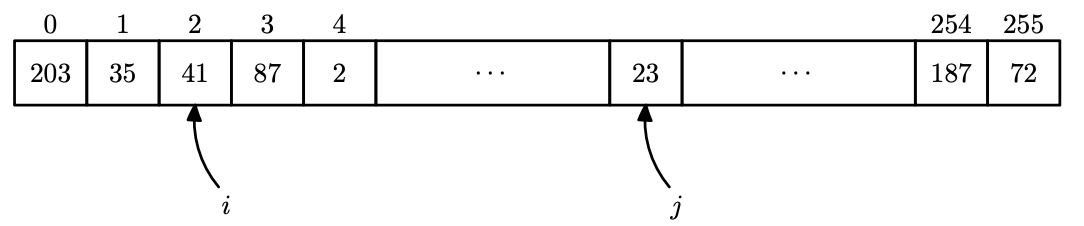
\includegraphics[width=0.75\linewidth]{figures/chapter3/fig12.png}
  \caption{RC4内部状态的一个例子}
  \label{fig:3-12}
\end{figure}

RC4流密码的密钥 $s$ 也是 PRG 的种子,用于将数组 $S$ 初始化为数字 $0 \dots 255$ 一个伪随机置换排列。初始化是使用下面的\textbf{设置算法(setup algorithm)}进行的:

\vspace*{5pt}

\hspace*{5pt} 输入:字节序列$s$

\vspace{3pt}

\hspace*{5pt} 对于 $i=1,\dots,255$:\\
\hspace*{50pt} 令 $S[i]\leftarrow i$ \\
\hspace*{26pt} 令 $j\leftarrow0$\\
\hspace*{26pt} 对于 $i=1,\dots,255$:\\
\hspace*{50pt} 令 $k\leftarrow s[i\;\mathrm{mod}\;|s|]$ \quad\quad // \emph{从种子中提取一个字节}\\
\hspace*{50pt} 令 $j\leftarrow(j+S[i]+k)\;\mathrm{mod}\;256$\\
\hspace*{50pt} $\mathrm{swap}(S[i],S[j])$

\vspace*{5pt}

在循环过程中,索引 $i$ 在数组中线性增长,而索引 $j$ 则跳来跳去。在每次迭代中,指针 $i$ 所指向的内容都会与 $j$ 所指向的内容互换。

一旦数组 $S$ 被初始化,PRG 就可以使用下面的\textbf{流生成器(stream generator)}一次生成一个字节的伪随机输出:

\vspace*{5pt}

\hspace*{5pt} 令 $i\leftarrow0$,$j\leftarrow0$\\
\hspace*{26pt} 重复:\\
\hspace*{50pt} 令 $i\leftarrow(i+1) \;\mathrm{mod}\;256$\\
\hspace*{50pt} 令 $j\leftarrow(j+S[i])\;\mathrm{mod}\;256$\\
\hspace*{50pt} $\mathrm{swap}(S[i],S[j])$ \\
\hspace*{50pt} 输出 $S\big[\,(S[i]+S[j])\;\mathrm{mod}\;256\,\big]$ \\
\hspace*{26pt} 直到永远

\vspace*{5pt}

该程序的运行时间视需要而定。同样地,索引 $i$ 在数组中线性增长,而索引 $j$ 则跳来跳去。交换 $S[i]$ 和 $S[j]$ 会不断地打乱数组 $S$。

\begin{snote}[RC4的加密速度。]
RC4 很适合用软件实现。其他流密码,如 Grain 和 Trivium,是为硬件设计的,在软件实现下的性能表现很差。表 \ref{tab:3-1} 提供了 RC4 和其他一些软件实现的流密码的运行时间对比。现代处理器运行在 $64$ 比特字长上,使得基于 $8$ 比特设计的 RC4 在这些架构上稍显缓慢。
\end{snote}

\begin{table}
  \centering
  \begin{tabular}{|c|c|}
    \hline
    密码 & 速度\footnotemark[1](MB/s)\\
    \hline
    RC4 & 126\\
    SEAL & 375\\
    Salsa20 & 408\\
    Sosemanuk & 727\\
    \hline
  \end{tabular}
  \caption{软件实现的流密码的速度比较(速度越高越好)。}
\end{table}

\subsection{RC4的安全性}

\footnotetext[1]{性能数字是使用 Crypto++ 5.6.0 benchmark 在 1.83 Ghz Intel Core 2 处理器上运行获得的。}

RC4一度被认为是一个安全的流密码,并被广泛部署在应用程序中。在一些攻击表明它的输出有一定的偏差后,该密码就失宠了。我们下面提出两种攻击,它们都能将 RC4 的输出与随机字符串区分开来。在本小节中,我们用$n$表示数组$S$的大小。对于RC4,我们有$n=256$。

\begin{snote}[初始 RC4 输出中的偏差。]
RC4的设置算法基于给定的随机种子将数组$S$初始化为$0 \dots 255$的一个置换。我们先暂且假设 RC4 的设置算法是完美的,它能从所有可能的 $256!$ 个排列组合中产生一个均匀的置换排列。Mantin和Shamir表明,即使假设初始化是完美的,RC4 的输出也是有偏差的。
\end{snote}

\begin{lemma}[Mantin-Shamir定理]\label{lemma:3-8}
假设数组 $S$ 被设置为 $0\dots n-1$ 的一个随机排列,并且 $i$ 和 $j$ 都被置为 $0$,那么 RC4 输出的第二个字节等于 $0$ 的概率为 $2/n$。
\end{lemma}

\begin{proof}[证明思路]
令$z_2$是 RC4 输出的第二个字节。令 $P$ 是 $S[2]=0$和 $S[1]\neq2$ 成立的事件。关键的观察是,当事件 $P$ 发生时,$z_2=0$ 的概率为 $1$,见图 \ref{fig:3-13}。然而,当 $P$ 没有发生时,$z_2$ 均匀分布在 $0\dots n-1$ 上,因此它等于 $0$ 的概率为 $1/n$。由于 $\Pr[P]$ 约为 $1/n$,我们可以得到以下(近似)结果:
\[
\begin{aligned}
\Pr[z_2=0] & =\Pr[(z_2=0)\;|\;P]\cdot\Pr[P]+\Pr[(z_2=0)\;|\;\neg P]\cdot\Pr[\neg P]\\
& \approx 1\cdot(1/n)+(1/n)\cdot(1-1/n)\approx2/n\qedhere
\end{aligned}
\]
\end{proof}

该引理表明,RC4输出的第二个字节为 $0$ 的概率是它本应有的两倍。这就导出了一个简单的 RC4 PRG 区分器。给定一个序列$x\in\{0,\dots,255\}^\ell$,对于$\ell\geq2$,如果$x$的第二个字节是$0$,区分器输出$0$,否则就输出$1$。根据引理 \ref{lemma:3-8},这个区分器的优势约为 $1/n$,对于 RC4 来说就是 $0.39\%$。

\begin{figure}
  \centering
  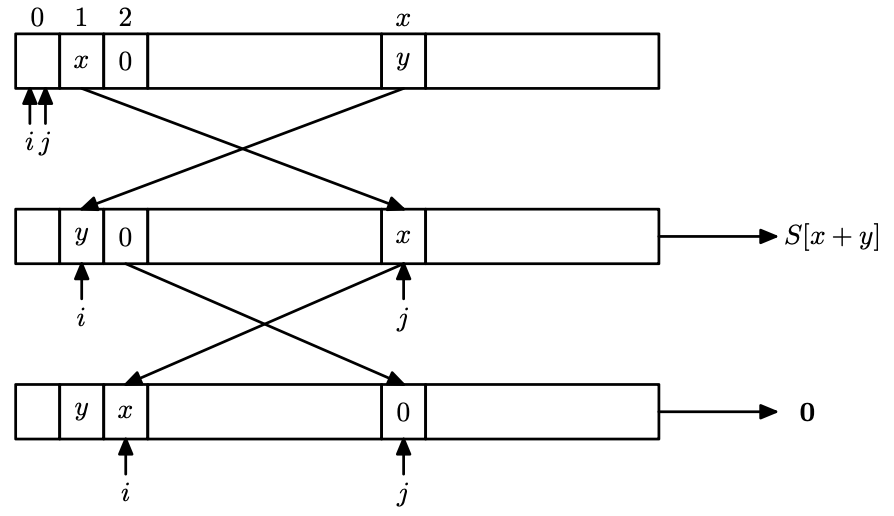
\includegraphics[width=0.55\linewidth]{figures/chapter3/fig13.png}
  \caption{引理 \ref{lemma:3-8} 的证明}
  \label{fig:3-13}
\end{figure}

Mantin-Shamir 区分器表明 RC4 输出的第二字节是有偏差的。AlFardan等人推广了这一结论,他们通过测量许多随机密钥上的偏差,表明输出的前$256$个字节中的每一个都有偏差:每个字节的分布都与均匀性相差甚远。这种偏差不像第二字节那样明显,但它仍是不可忽略不计的,足以用来对密码发动攻击。例如,他们表明,给定用 $2^{30}$ 个随机密钥加密的单一明文的对应密文,我们有可能以接近 $1$ 的概率恢复明文的前 $128$ 字节。这种攻击很容易在网络上进行,因为在网络上,一个秘密的 cookie 通常被嵌入到一个消息的前几个字节中。每次浏览器连接到受害者的网络服务器时,这个 cookie 都会用新的密钥重新加密。攻击者可以使用 Javascript 脚本令用户的浏览器反复重连到目标网站,以向攻击者提供发动攻击和暴露 cookie 所需的 $2^{30}$ 个密文。

作为回应,RSA实验室发布了一项建议,建议放弃RC4流生成器输出的前 $1024$ 字节,而只使用第 $1025$ 字节及以后的字节。这可以防御最初的密钥流偏差区分器,但不能防御我们接下来将要讨论的攻击。

\begin{snote}[RC4流生成器中的偏差。]
假设RC4设置算法已经被修改,从而使得上面介绍的攻击无效。Fluhrer和McGrew给出了一个直接针对流生成器的攻击。他们声称字节对$(0,0)$ 在 RC4 的输出中出现的次数多于它应该在随机序列中出现的次数。这足以将 RC4 的输出与随序列区分开来。

令 $\mathrm{ST}_\mathrm{RC4}$ 为 RC4 所有可能的内部状态的集合。由于数组 $S$ 有 $n$ 个可能的设置,$i$ 和 $j$ 各有 $n$ 个可能的设置,所以 $\mathrm{ST}_\mathrm{RC4}$ 的大小为 $n!\cdot n^2$。由于在 RC4 中$n=256$,$\mathrm{ST}_\mathrm{RC4}$ 的大小是非常巨大的,大约为 $10^{511}$。
\end{snote}

\begin{lemma}[Fluhrer-McGrew定理]
假设RC4使用一个$\mathrm{ST}_\mathrm{RC4}$中的随机状态$T$初始化。令$(z_1,z_2)$是 RC4 在状态 $T$ 下启动时输出的前两个字节。则有:
\[
\begin{aligned}\label{lemma:3-9}
& i\neq n−1 & \Longrightarrow & \quad\Pr[(z_1,z_2)=(0,0)]\geq(1/n^2)\cdot\big(1+(1/n)\big)\\
& i\neq 0,1 & \Longrightarrow & \quad\Pr[(z_1,z_2)=(0,1)]\geq(1/n^2)\cdot\big(1+(1/n)\big)
\end{aligned}
\]
\end{lemma}

我们将一对连续输出 $(z_1,z_2)$ 称为一个\textbf{二重字(digraph)}。在一个真正的随机序列中,所有二重字$(x,y)$出现的概率都应当正好是 $1/n^2$。上面的引理表明,对于RC4,$(0,0)$出现的概率比它应有的值大$1/n^3$。$(0,1)$也是如此。事实上,除了引理 \ref{lemma:3-9} 所述的两个二重字,Fluhrer-McGrew 还确定了其他几个异常的二重字。

该引理导出了一个简单的区分 RC4 的输出和随机序列的区分器 $D$。如果区分器在给定的序列中发现的 $(0,0)$ 的数量大于随机序列中应有的数量,它就输出 $1$,否则就输出 $0$。

\vspace*{5pt}

\hspace*{5pt} 输入:序列$s\in\{0,\dots,n\}^\ell$\\
\hspace*{26pt} 输出:$0$ 或 $1$

\vspace{3pt}

\hspace*{5pt} 令 $q$ 为 $x$ 中出现二重字 $(0,0)$ 的次数\\
\hspace*{26pt} 如果 $(q/\ell)-(1/n^2)>1/(2n^3)$ 则输出 $0$,否则输出 $1$

\vspace*{5pt}

使用定理 \ref{theo:B-3},我们可以估计出 $D$ 的优势与输入长度 $\ell$ 的关系。特别地,区分器 $D$ 能获取下述优势:
\[
\begin{aligned}
\ell=2^{14}\text{ 字节}: &\quad\quad \mathrm{PRG}\mathsf{adv}[D,RC4]\geq2^{-8}\\
\ell=2^{34}\text{ 字节}: &\quad\quad \mathrm{PRG}\mathsf{adv}[D,RC4]\geq0.5
\end{aligned}
\]
使用Fluhrer和McGrew提供的所有异常二重字,我们就可以建立一个区分器,只用 $2^{30.6}$ 字节的输出就能实现 $0.8$ 的优势。

\begin{snote}[对RC4的相关密钥攻击。]
Fluhrer、Mantin和Shamir表明,RC4 与相关密钥一起使用时是不安全的。我们将在 \ref{sec:9-10} 节的攻击 $2$ 中讨论这种攻击及其对 802.11b WiFi 协议的影响。
\end{snote}
\section{在实践中生成随机比特}

在密码学中,许多任务都需要随机比特,例如生成密钥和其他被称为 nonce 的短时值。在整本书中,我们假设所有参与方都能获得良好的随机源,否则许多理想的密码学目标就都不可能实现。到目前为止,我们使用 PRG 将一个短的均匀分布的秘密种子拉伸成一个长的伪随机序列。虽然 PRG 是生成伪随机比特序列的一个重要工具,但它只是故事的一部分。

在实践中,随机比特序列通常是使用\textbf{随机数生成器 (random number generator, RNG)} 生成的。RNG 和 PRG 一样输出一串随机或伪随机的比特。然而 RNG 有一个额外的接口,用于不断向 RNG 的内部状态添加熵,如图 \ref{fig:3-14} 所示。其原理是,每当系统有更多的随机熵贡献给 RNG 时,这些熵就被添加到 RNG 的内部状态中。每当有人从 RNG 中读取比特时,这些比特都是用当前的内部状态生成的。

\begin{figure}
  \centering
  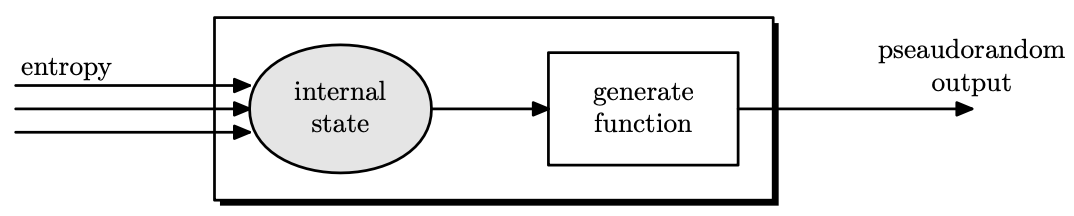
\includegraphics[width=0.7\linewidth]{figures/chapter3/fig14.png}
  \caption{一个随机数生成器}
  \label{fig:3-14}
\end{figure}

一个典型的例子是 Linux 操作系统中的 RNG,它被实现成一个名为 \texttt{/dev/random} 的设备。任何人都可以从该设备中读取到随机比特。你可以在 UNIX shell 中输出 \texttt{cat /dev/random} 来试着玩一玩这个工具,你将会看到一串无休止的、看起来很随机的字符。UNIX RNG 从一些硬件来源获得随机熵,包括:
\begin{itemize}
	\item 键盘事件:按键时间间隔能够提供随机熵;
	\item 鼠标事件:中断时间和鼠标位置都能够提供随机熵;
	\item 硬件中断:硬件中断的时间间隔也能提供较高质量的随机熵。
\end{itemize}
这些随机源能够产生连续的随机流,并会被定期异或到 RNG 的内部状态上。请注意,具体的键盘输入内容不会被用作熵的来源,通常使用的只是按键的时间,这是为了确保用户的输入内容不会通过 RNG 泄露给系统中的其他用户。

\begin{snote}[高熵的随机生成。]
上述熵源产生随机流的速度相对较慢。为了以更快的速度生成真随机比特,英特尔从 2012 年的 Ivy Bridge 处理器系列开始,增加了一个硬件随机数生成器。使用 \texttt{RdRand} 指令即可读取这个生成器的输出,它旨在提供一个快速且均匀的随机比特生成器。

为了减少生成器输出中的偏差,原始比特首先通过一个被称为``调节器"的函数,以确保在提供足够熵源作为输入时,输出是一个均匀分布的比特序列。我们在 \ref{sec:8-10} 节讨论密钥推导问题时会更详细地讨论这个问题。

\texttt{RdRand} 发生器不应该取代其他的熵源,比如上面描述的几个熵源;它只应该作为 RNG 的一个\emph{额外的}熵源来增强它们。这样一来,如果生成器有缺陷,就不会完全影响到加密应用。

英特尔的方法的一个困难是,随着时间的推移,被采样的硬件元素可能由于硬件故障而停止产生随机流。例如,被采样的比特可能总是 ``$0$",这会导致高度非随机的输出。为了防止这种情况的发生,RNG 的输出会被不断地用一套固定的统计方法来测试。如果任何一项测试报告为``非随机",发生器就会被认为有缺陷。
\end{snote}
\section{一个更广阔的视角:计算上不可区分性}

我们对伪随机数发生器 $G$ 的安全性的定义将下面这个直观的想法进行了形式化,即对手不应该能够有效区分 $G(s)$ 和 $r$,其中 $s$ 是一个随机选出的种子,而 $r$ 是输出空间中的一个随机元素。

这个想法可以很自然地推广到其他场合。假设 $P_0$ 和 $P_1$ 是有限集 $\mathcal{R}$ 上的两个概率分布。我们的目标是定义一个直观的概念,即对手无法有效地区分 $P_0$ 和 $P_1$。与之前一样,这通过设计一个攻击游戏来完成。对于 $b=0,1$,我们记 $x\overset{\rm R}\leftarrow P_b$ 为根据概率分布 $P_b$ 从集合 $\mathcal R$ 中随机选出一个值赋给 $x$。

\begin{game}[区分 $P_0$ 和 $P_1$]\label{game:3-3}
对于有限集 $\mathcal{R}$ 上的给定概率分布 $P_0$ 和 $P_1$ 以及一个给定对手 $\mathcal A$,我们定义两个实验:实验 $0$ 和实验 $1$。对于 $b=0,1$,我们定义:

\noindent\textbf{实验 $b$:}
\begin{itemize}
	\item 挑战者计算 $x\overset{\rm R}\leftarrow P_b$,并将 $x$ 发送给对手。
	\item 给定 $x$,对手计算并输出一个比特 $\hat b\in\{0,1\}$。
\end{itemize}

对于 $b=0,1$,令 $W_b$ 为对手 $\mathcal A$ 在实验 $b$ 中输出 $1$ 的事件。 我们定义 $\mathcal A$ 相对于 $P_0$ 和 $P_1$ 的\textbf{优势}为:
\[
\mathrm{Dist}\mathsf{adv}[\mathcal{A},P_0,P_1]:=\big\lvert\Pr[W_0]-\Pr[W_1]\big\rvert
\]
\end{game}

\begin{definition}[计算上不可区分性]\label{def:3-4}
如果 $\mathrm{Dist}\mathsf{adv}[\mathcal{A},P_0,P_1]$ 的值对任意有效对手 $\mathcal A$ 来说均可忽略不计,则称概率分布 $P_0$ 和 $P_1$ \textbf{在计算上不可区分 (computationally indistinguishable)}。
\end{definition}

利用该定义,我们可以更简单地重新表述安全 PRG 的定义:如果 $P_1$ 是 $\mathcal R$ 上的均匀分布,$P_0$ 是对 $r\in\mathcal R$ 的赋值的概率分布:
\[
P_0(r):=\frac{|\{s\in\mathcal{S}:G(s)=r\}|}{|\mathcal{S}|}
\]
当且仅当 $P_0$ 和 $P_1$ 在计算上不可区分时,定义在 $(\mathcal S,\mathcal R)$ 上的 PRG 是安全的。

与 \ref{subsec:2-2-5} 中讨论的相同,攻击游戏 \ref{game:3-3} 可以被改写为一个``比特猜测"游戏,其中挑战者不再有两个独立的实验,而是随机选择一个 $b\in\{0,1\}$,然后与对手 $\mathcal A$ 运行实验 $b$。在这个游戏中,我们将 $\mathcal A$ 的\emph{比特猜测优势}$\mathrm{Dist}\mathsf{adv}^*[\mathcal{A},P_0,P_1]$记为$|\Pr[\hat b=b]-{1}/{2}|$。那么 \ref{subsec:2-2-5} 中的推广结论(即式 \ref{eq:2-11})也适用于此:
\begin{equation}
{\rm Dist\mathsf{adv}}[\mathcal{A},P_0,P_1]=2\cdot\mathrm{Dist}\mathsf{adv}^*[\mathcal{A},P_0,P_1]
\end{equation}

通常情况下,为了证明两个分布在计算上是不可区分的,我们不得不做某些其他的计算上的假设。然而有时两个分布真的极其相似,以至于无论对手有多么强大的计算能力,都无法有效区分它们。为了准确表述这种``相似性"的概念,我们下面将引入一个有用的工具,称为\textbf{统计距离 (statistical distance)}:

\begin{definition}[统计距离]\label{def:3-5}
假设 $P_0$ 和 $P_1$ 是有限集 $\mathcal R$ 上的概率分布,那么它们的\textbf{统计距离}定义为:
\[
\Delta[P_0,P_1]:=\frac{1}{2}\sum_{r\in\mathcal{R}}\big\lvert P_0(r)-P_1(r)\big\rvert
\]
\end{definition}

\begin{example}\label{exmp:3-1}
假设 $P_0$ 是 $\{1,\dots,m\}$ 上的均匀分布,$P_1$ 是 $\{1,\dots,m-\delta\}$ 上的均匀分布,其中 $\delta\in\{0,\dots,m-1\}$。我们下面试着计算 $\Delta[P_0,P_1]$。我们固然可以直接使用统计距离的定义来计算 $\Delta[P_0,P_1]$;但是,不妨考虑下面这张关于 $P_0$ 和 $P_1$ 的图:

\begin{figure*}[h!]
  \centering
  \input{figures/chapter3/vac1.tex}
\end{figure*}

$P_0$ 和 $P_1$ 的统计距离就是图中区域 $A$ 和区域 $C$ 面积和的一半。此外,由于概率分布的总和为 $1$,我们必然有:
\[
\text{area of } B+ \text{area of } A= 1 = \text{area of } B+ \text{area of } C
\]
因此区域 $A$ 和区域 $C$ 的面积相等。所以:
\[
\Delta[P_0,P_1]=\text{area of } A = \text{area of } C ={\delta}/{m}
\]
\end{example}

下面的定理使我们能够在计算上不可区分性和统计距离这两个概念之间建立起联系。

\begin{theorem}\label{theo:3-10}
令 $P_0$ 和 $P_1$ 是有限集 $\mathcal R$ 上的两个概率分布,那么我们有:
\[
\max_{\mathcal{R}'\subseteq\mathcal{R}}|P_0[\mathcal{R}']-P_1[\mathcal{R}']|=\Delta[P_0,P_1]
\]
其中,最大值在 $\mathcal R$ 的所有子集 $\mathcal R'$ 上都能取得。
\end{theorem}

\begin{proof}
假设我们把 $\mathcal{R}$ 分成两个互不相干的子集:由使得 $P_0(r)<P_1(r)$ 的 $r\in\mathcal R$ 组成的集合 $\mathcal{R}_0$,以及由使得 $P_0(r)\geq P_1(r)$ 的 $r\in\mathcal R$ 组成的集合 $\mathcal{R}_1$。考虑下面的 $P_0$ 和 $P_1$ 分布的示意图,其中 $\mathcal{R}_0$ 的元素被放在 $\mathcal{R}_1$ 的元素的左边:

\begin{figure*}[h!]
  \centering
  \input{figures/chapter3/vac2.tex}
\end{figure*}

现在,与例 \ref{exmp:3-1} 中一样,我们有:
\[
\Delta[P_0,P_1]=\text{area of } A = \text{area of } C
\]
注意到,对于 $\mathcal{R}$ 的每个子集 $\mathcal{R}'$,我们都有:
\[
P_0[\mathcal{R}']-P_1[\mathcal{R}']=\text{area of } C' - \text{area of } A'
\]
其中 $C'$ 指位于 $\mathcal{R}'$ 上的 $C$ 的子区域,$A'$ 指位于 $\mathcal{R}'$ 上的 $A$ 的子区域。由此可知,当 $\mathcal{R}'=\mathcal{R}_0$ 或 $\mathcal{R}'=\mathcal{R}_1$ 时,$|P_0[\mathcal{R}']-P_1[\mathcal{R}']|$ 取得最大值,此时最大值就等于 $\Delta[P_0,P_1]$。
\end{proof}

与计算上不可分性的联系如下:

\begin{theorem}\label{theo:3-11}
假设 $P_0$ 和 $P_1$ 是有限集 $\mathcal{R}$ 上的概率分布,那么对于任意对手 $\mathcal A$,我们都有:
\[
{\rm Dist\mathsf{adv}}[\mathcal{A},P_0,P_1]\leq\Delta[P_0,P_1]
\]
\end{theorem}

\begin{proof}
考虑一个如攻击游戏 \ref{game:3-3} 中那样试图区分 $P_0$ 和 $P_1$ 的对手 $\mathcal A$。

首先,我们考虑 $\mathcal A$ 是确定性算法的情况。在这种情况下,$\mathcal A$ 的输出是一个 $r\in\mathcal{R}$ 的函数 $f(r)$,它是由挑战者发送给 $\mathcal A$ 的。令 $\mathcal{R}':=\{r\in\mathcal{R}:f(r)=1\}$。如果 $W_0$ 和 $W_1$ 是攻击游戏 \ref{game:3-3} 中定义的两个事件,那么对于 $b=0,1$,我们有:
\[
\Pr[W_b]=P_b[\mathcal{R}']
\]
根据定理 \ref{theo:3-10},我们有:
\[
{\rm Dist\mathsf{adv}}[\mathcal{A},P_0,P_1]=|P_0[\mathcal{R}']-P_1[\mathcal{R}']|\leq\Delta[P_0, P_1]
\]

我们下面考虑 $\mathcal A$ 是概率性算法的情况。我们可以认为 $\mathcal A$ 接受一个辅助输入 $t$ ,代表它的随机选择。我们认为 $t$ 是从某个有限集 $\mathcal{T}$ 中均匀随机选出的。因此,$\mathcal A$ 的输出是挑战者交给它的值 $r\in\mathcal{R}$ 和代表其随机选择的值 $t\in\mathcal{T}$ 的函数 $g(r,t)$。对于一个给定的 $t\in\mathcal{T}$,令 $\mathcal{R}_t':=\{r\in\mathcal{R}:g(r,t)=1\}$。然后,对 $t$ 的随机选择进行平均化,我们有:
\[
\Pr[W_b]=\frac{1}{|\mathcal{T}|}\sum_{t\in\mathcal{T}}P_b[\mathcal{R}_t']
\]
由此可得:
\[
\begin{aligned}
{\rm Dist\mathsf{adv}}[\mathcal{A},P_0,P_1]
&=|P_0[\mathcal{R}']-P_1[\mathcal{R}']|\\
&=\frac{1}{|\mathcal{T}|}\bigg\lvert\sum_{t\in\mathcal{T}}(P_0[\mathcal{R}_t']-P_1[\mathcal{R}_t'])\bigg\rvert\\
&\leq\frac{1}{|\mathcal{T}|}\sum_{t\in\mathcal{T}}|P_0[\mathcal{R}_t']-P_1[\mathcal{R}_t']|\\
&\leq\frac{1}{|\mathcal{T}|}\sum_{t\in\mathcal{T}}\Delta[P_0,P_1]\\
&=\Delta[P_0,P_1]\qedhere
\end{aligned}
\]
\end{proof}

作为该定理的一个结论,我们可以看到,如果 $\Delta[P_0,P_1]$ 可忽略不计,那么 $P_0$ 和 $P_1$ 是计算上不可区分的。

\vspace{5pt}

我们还可以将两个随机变量之间的统计距离定义为它们相应分布之间的统计距离。也就是说,如果 $\mathsf{X}$ 和 $\mathsf{Y}$ 是在一个有限集 $\mathcal{R}$ 中取值的随机变量,那么它们的\textbf{统计距离}是:
\[
\Delta[\mathsf{X},\mathsf{Y}]
:=
\frac{1}{2}
\sum_{r\in\mathcal{R}}
|\Pr[\mathsf{X}=r]-Pr[\mathsf{Y}=r]|
\]
在这种情况下,定理 \ref{theo:3-10} 表明:
\[
\max_{\mathcal{R}'\subseteq\mathcal{R}}
|\Pr[\mathsf{X}\in\mathcal{R}']-\Pr[\mathsf{Y}\in\mathcal{R}']|=\Delta[\mathsf{X},\mathsf{Y}]
\]
其中,最大值在 $\mathcal R$ 的所有子集 $\mathcal R'$ 上都能取得。

类似地,我们还可以对随机变量而非分布来定义区分优势。使用随机变量的好处是,我们可以更方便地处理彼此相关的分布,正如下面的定理所例证的那样。

\begin{theorem}\label{theo:3-12}
如果 $\mathcal{S}$ 和 $\mathcal{T}$ 是有限集,$\mathsf{X}$ 和 $\mathsf{Y}$ 是在 $\mathcal{S}$ 上取值的随机变量,并且 $f:\mathcal{S}\to\mathcal{T}$ 是一个函数,那么 $\Delta[f(\mathsf{X}),f(\mathsf{Y})]\leq\Delta[\mathsf{X},\mathsf{Y}]$。
\end{theorem}

\begin{proof}
对于某个 $\mathcal{T}'\subseteq\mathcal{T}$,我们有:
\[
\begin{aligned}
\Delta[f(\mathsf{X}),f(\mathsf{Y})]
&=|\Pr[f(\mathsf{X})\in\mathcal{T}']-\Pr[f(\mathsf{Y})\in\mathcal{T}']|\quad\text{\emph{(根据定理} \ref{theo:3-10}\emph{\,)}}\\
&=|\Pr[\mathsf{X}\in f^{-1}(\mathcal{T}')]-\Pr[\mathsf{Y}\in f^{-1}(\mathcal{T}')]|\\
&\leq\Delta[\mathsf{X},\mathsf{Y}]\quad\text{\emph{(根据定理} \ref{theo:3-10}\emph{\,)}}\qedhere
\end{aligned}
\]
\end{proof}

\begin{example}\label{exmp:3-2}
令 $\mathsf{X}$ 均匀分布在集合 $\{0,\dots,m-1\}$ 上,$\mathsf{Y}$ 均匀分布在集合 $\{0,\dots,N-1\}$ 上,且 $N\geq m$。令 $f(t):=t\;\mathrm{mod}\;m$。我们想计算 $\mathsf{X}$ 和 $f(\mathsf{Y})$ 之间的统计距离的上界。我们可以这样做。令 $N=qm-r$,其中 $0\leq r<m$,因此 $q=\lceil{N}/{m}\rceil$。同时,令 $\mathsf{Z}$ 均匀分布在集合 $\{0,\dots,qm-1\}$ 上。那么 $f(\mathsf{Z})$ 就均匀分布在集合 $\{0,\dots,m-1\}$ 上,这是因为 $\{0,\dots,m-1\}$ 中的每个元素在函数 $f$ 下都有相同个数的原像(即$q$个),这些原像都落在集合 $\{0,\dots,qm-1\}$ 中。由于统计距离只取决于随机变量的分布,根据定理 \ref{theo:3-12},我们有:
\[
\Delta[\mathsf{X},f(\mathsf{Y})]=\Delta[f(\mathsf{Z}),f(\mathsf{Y})]\leq\Delta[\mathsf{Z},\mathsf{Y}]
\]
正如我们在例 \ref{exmp:3-1} 中所看到的:
\[
\Delta[\mathsf{Z},\mathsf{Y}]=\frac{r}{qm}<\frac{1}{q}\leq\frac{m}{N}
\]
因此有:
\[
\Delta[\mathsf{X},f(\mathsf{Y})]<\frac{m}{N}
\]
\end{example}

\begin{example}
现在我们想要生成一个给定区间 $\{0,\dots,m-1\}$ 上的伪随机数。假设我们有一个PRG $G$,它可以输出 $L$ 比特的序列。当然,一个 $L$ 比特的序列可以被看作是 $\{0,\dots,N-1\}$ 中的一个数,其中 $N:=2^L$。让我们假设 $N\geq m$。

为了生成一个区间 $\{0,\dots,m-1\}$ 上的伪随机数,我们可以把 $G$ 的输出看作是 $\{0,\dots,N-1\}$ 中的一个数,并将其模 $m$ 后输出。我们下面将表明,只要 $G$ 是安全的,且 ${m}/{N}$ 可忽略不计,上述方法所产生的数和从区间 $\{0,\dots,m-1\}$ 中随机挑选的真随机数在计算上不可区分。

为此,令 $P_0$ 为 $G$ 输出并模 $m$ 后的分布,$P_1$ 为 $\{0,\dots,m-1\}$ 上的均匀分布,令 $\mathcal A$ 是一个试图区分 $P_0$ 和 $P_1$ 的对手,就像在攻击游戏 \ref{game:3-3} 中的那样。

令游戏 $0$ 为攻击游戏 \ref{game:3-3} 中的实验 $0$,在这个实验中,$\mathcal A$ 被赋予了一个按照 $P_0$ 分布的随机样本,记 $W_0$ 是 $\mathcal A$ 在游戏 $0$ 中输出 $1$ 的事件。

现在,定义游戏 $1$ 与游戏 $0$ 基本相同,只是我们用一个从区间 $\{0,\dots,N-1\}$ 中随机选出的真随机数代替 $G$ 的输出。记 $W_1$ 为 $\mathcal A$ 在游戏 $1$ 中输出 $1$ 的事件。我们很容易构建出一个有效对手 $\mathcal{B}$,它可以像攻击游戏 \ref{game:3-1} 中那样攻击 $G$,并使得:
\[
{\rm PRG\mathsf{adv}}[\mathcal{B},G]=|{\rm Pr}[W_0]-{\rm Pr}[W_1]|
\]
思路是 $\mathcal{B}$ 获取到它的挑战值并模 $m$,然后将这个值交给 $\mathcal A$,然后原样输出 $\mathcal A$ 输出的任何东西。

最后,我们定义游戏 $2$ 为攻击游戏 \ref{game:3-3} 中的实验 $1$,在这个实验中,$\mathcal A$ 被赋予了一个按照 $P_1$ 分布的随机样本,也就是 $\{0,\dots,m-1\}$ 上的均匀分布。记 $W_2$ 为 $\mathcal A$ 在游戏 $2$ 中输出 $1$ 的事件。如果 $P$ 是游戏 $1$ 中交给 $\mathcal A$ 的值的分布,那么根据定理 \ref	{theo:3-11},我们就有 $|\Pr[W_1]-\Pr[W_2]|\leq\Delta[P,P_1]$;此外,根据例 \ref{exmp:3-2},我们还有 $\Delta[P,P_1]\leq{m}/{N}$。

将以上结论综合起来,可以得到:
\[
\begin{aligned}
{\rm Dist\mathsf{adv}}[\mathcal{A},P_0,P_1]
&=|\Pr[W_0]-\Pr[W_2]|\leq|\Pr[W_0]-\Pr[W_1]|+|\Pr[W_1]-\Pr[W_2]|\\
&\leq{\rm PRG\mathsf{adv}}[\mathcal{B},G]+\frac{m}{N}
\end{aligned}
\]
而根据假设,该值可忽略不计。
\end{example}

\subsection{数学细节}

和之前一样,我们下面会详述相关的数学细节,以便从渐进复杂性理论的角度解释本节的定义和结论。

在定义计算上不可区分性(定义 \ref{def:3-4})时,我们应该考虑两个概率分布族 $P_0=\{P_{0,\lambda}\}_{\lambda}$ 和 $P_1=\{P_{1,\lambda}\}_{\lambda}$,它们都由安全参数 $\lambda$ 索引。对于每个 $\lambda$,分布 $P_{0,\lambda}$ 和 $P_{1,\lambda}$ 都应该在有限比特序列集合 $\mathcal{R}_\lambda$ 中取值,其中 $\mathcal{R}_\lambda$ 中的序列长度以 $\lambda$ 的多项式为界。 在攻击游戏 \ref{game:3-3} 中,安全参数 $\lambda$ 是挑战者和对手的输入,而在实验 $b$ 中,挑战者产生一个根据 $P_{b,\lambda}$ 分布的样本。优势应当被正确地表记为 ${\rm Dist\mathsf{adv}}[\mathcal{A},P_0,P_1](\lambda)$,它是 $\lambda$ 的一个函数,而计算上不可区分性意味着该函数可以忽略不计。

在某些情况下,引入一个概率生成的系统参数可能是很自然的;然而,从技术角度来看,这不是必要的,因为这样的系统参数可以被纳入到分布 $P_{0,\lambda}$ 和 $P_{1,\lambda}$ 中。我们还可以要求 $P_{0,\lambda}$ 和 $P_{1,\lambda}$ 是可有效采样的;然而,为了保持定义的简单性,我们不会强制要求这样做。

统计距离的定义(定义 \ref{def:3-5})从非渐进的角度来看是完全合理的,不需要任何修改或阐述。如前所述,定理 \ref{theo:3-10} 对特定的分布 $P_0$ 和 $P_1$ 成立。定理 \ref{theo:3-11} 可以渐进地看作是说,对于所有分布族 $P_0=\{P_{0,\lambda}\}_{\lambda}$ 和 $P_1=\{P_{1,\lambda}\}_{\lambda}$,对于任意对手(甚至是计算上无界的对手),以及对于所有 $\lambda$,我们都有:
\[
{\rm Dist\mathsf{adv}}[\mathcal{A},P_0,P_1](\lambda)\leq\Delta[P_{0,\lambda},P_{1,\lambda}]
\]
\section{一个有趣的应用:抛掷硬币与比特承诺}\label{sec:3-12}

Alice 和 Bob 要出去约会了。Alice 想看某一部电影,而 Bob 想看另一部。他们决定抛一枚硬币来随机选择电影。如果抛硬币的结果是正面,他们就去看 Alice 选择的电影,否则就去看 Bob 选择的电影。当 Alice 和 Bob 离得很近的时候,这很容易操作:他们中的一个人,比如说 Bob,抛出一枚硬币,他们都能验证这个结果。但当他们相距甚远,并且在电话中交谈时,这就比较难了。Bob 可以在他那边掷硬币,然后告诉 Alice 结果,但是 Alice 却没有理由相信这个结果。Bob 可以简单地声称抛硬币的结果是反面,而 Alice 则没有办法证实这一点。这不是一个开始约会的好方法。

解决这个问题的一个简单方法是利用一种叫做\textbf{比特承诺(bit commitment)}的密码学原语。它能够让 Bob 承诺一个他选择的比特 $b\in\{0,1\}$。稍后,Bob 可以打开承诺,让 Alice 相信 $b$ 是 Bob 所承诺的值。承诺一个比特 $b$ 会产生一个\textbf{承诺序列(commitment string)} $c$,它会被 Bob 发送给 Alice;还会产生一个\textbf{打开序列(opening string)},它在之后会被 Bob 用于打开承诺。如果一个承诺方案满足以下两个特性,它就是安全的:
\begin{itemize}
	\item \textbf{隐藏(hiding)}:承诺序列 $c$ 不会透露关于承诺比特 $b$ 的任何信息。更确切地说,承诺比特为 $0$ 时 $c$ 的分布与承诺比特为 $1$ 时 $c$ 的分布是不可区分的。在我们提出的比特承诺方案中,隐藏属性取决于特定的 PRG $G$ 的安全性。
	\item \textbf{绑定(binding)}:令 $c$ 是 Bob 输出的承诺序列。如果 Bob 可以将该承诺打开为某个 $b\in\{0,1\}$,他就不能将其打开为 $\bar{b}$。这就保证了,一旦 Bob 承诺了一个比特 $b$,他就只可以把它打开为 $b$,而不能是其他的值。在我们提出的承诺方案中,绑定属性无条件成立。
\end{itemize}

\begin{snote}[抛掷硬币。]
使用一个承诺方案,Alice 和 Bob 就可以生成一个随机比特 $b\in\{0,1\}$,这样,假设协议成功终止,任何一方都不能使结果朝着自己的方向偏移。这样的协议被称为\textbf{抛掷硬币协议(coin flipping protocols)}。结果比特 $b$ 将决定他们去看什么电影。

Alice 和 Bob 使用下面这个简单的抛掷硬币协议:

\vspace*{10pt}

\hspace*{5pt} 步骤 1:Bob 随机选择一个比特 $b_0\overset{\rm R}\leftarrow\{0,1\}$。\\
\hspace*{66pt} Alice 和 Bob 执行承诺协议。\\
\hspace*{66pt} 通过该协议,Alice 获得对 $b_0$ 的承诺 $c$,Bob 获得一个打开序列 $s$。\\
\hspace*{26pt} 步骤 2:Alice 随机选择一个比特 $b_1\overset{\rm R}\leftarrow\{0,1\}$,并将其明文发送给 Bob。\\
\hspace*{26pt} 步骤 3:Bob 通过向 Alice 揭露 $b_0$ 和 $s$ 来打开承诺。\\
\hspace*{66pt} Alice 验证 $c$ 是否是对 $b_0$ 的承诺,如果验证失败则终止。

\vspace*{5pt}

\hspace*{5pt} 输出:结果比特 $b:=b_0\oplus b_1$。

\vspace*{10pt}

\noindent
我们声称,如果协议成功终止,并且一方诚实地遵守协议,那么另一方就不能使结果朝它的倾向偏移。根据隐藏属性,Alice 在步骤 $1$ 结束时不会得到任何关于 $b_0$ 的信息,因此她对 $b_1$ 的选择与 $b_0$ 的值无关。根据绑定属性,Bob 只能在步骤 $3$ 中对他在步骤 $1$ 中选择的 $b_0$ 打开承诺 $c$。而由于他在 Alice 选择 $b_1$ 之前就选择了 $b_0$,所以 Bob 对 $b_0$ 的选择与 $b_1$ 无关。我们可以得出结论,输出比特 $b$ 是两个独立比特的异或。因此,如果一方诚实地遵守协议,另一方就不可能使产生的比特有所偏向。

这个协议的一个问题是,Bob 在步骤 $2$ 结束时,在 Alice 获取比特之前就知道了生成的比特。原则上,如果结果不是 Bob 想要的,他也可以在步骤 $2$ 结束时中止协议,并试图重新启动协议,并且期待下一次运行能得到他想要的结果。更复杂的抛掷硬币协议能够避免这个问题,但代价是需要更多回合的交互(比如,参见 \cite{moran2009optimally})。
\end{snote}

\begin{snote}[来自安全PRG的比特承诺。]
剩下的工作就是构建一个让 Bob 承诺他的比特 $b_0\in\{0,1\}$ 的安全比特承诺方案。我们使用 Naor 提出的一个优雅的构造来完成这个工作 \cite{naor1989bit}。

令 $G:\mathcal{S}\to\mathcal{R}$ 是一个安全的 PRG,其中 $|\mathcal{R}|\geq|\mathcal{S}|^3$,$\mathcal{R}=\{0,1\}^n$,$n$ 是某个正整数。为了承诺比特 $b_0$,Alice 和 Bob 参与以下协议:

\vspace*{5pt}

\hspace*{5pt} Bob 承诺比特 $b_0\in\{0,1\}$:\\
\hspace*{50pt} 步骤 1:Alice 随机选择一个 $r\in\mathcal{R}$,并将 $r$ 发送给 Bob。\\
\hspace*{50pt} 步骤 2:Bob 随机选择一个 $s\in\mathcal{S}$ 并计算 $c\leftarrow\mathrm{com}(s,r,b_0)$\\
\hspace*{90pt} 其中 $\mathrm{com}(s,r,b_0)$ 是以下函数:\\
\[
c=\mathrm{com}(s,r,b_0):=
\left\{
\begin{array}{ll}
G(s), & b_0=0\\
G(s)\oplus r, & b_0=1
\end{array}	
\right.
\]

\hspace*{5pt} Bob 输出 $c$ 作为承诺序列,并将 $s$ 作为打开序列。

\vspace*{5pt}

\noindent
当到了打开承诺的时候,Bob 将 $(b_0,s)$ 发送给 Alice。如果 $c=\mathrm{com}(s,r,b_0)$ 成立,Alice 就接受打开值,否则就拒绝它。

隐藏属性直接来自于 PRG 的安全性:因为输出 $G(s)$ 与 $\mathcal{R}$ 上的均匀随机序列在计算上是不可区分的,所以 $G(s)\oplus r$ 与 $\mathcal{R}$ 上的均匀随机序列在计算上也是不可区分的。因此,无论是 $b_0=0$ 还是 $b_0=1$,承诺序列 $c$ 与 $\mathcal{R}$ 上的均匀序列在计算上都是不可区分的,正如所要求的那样。

只要 $1/|\mathcal{S}|$ 可忽略不计,绑定属性就无条件成立。Bob 可以将一个承诺 $c\in\mathcal{R}$ 打开为 $0$ 和 $1$ 的唯一办法,就是找到两个种子 $s_0,s_1\in\mathcal{S}$ 满足 $c=G(s_0)=G(s_1)\oplus r$,这意味着 $G(s_0)\oplus G(s_1)=r$。如果存在种子 $s_0,s_1\in\mathcal{S}$ 满足 $G(s_0)\oplus G(s_1)=r$,我们就称这样的 $r\in\mathcal{R}$ 是``坏的"。种子对 $(s_0,s_1)$ 的数量是 $|\mathcal{S}|^2$,因此坏的 $r$ 的数量最多也是 $|\mathcal{S}|^2$。由此可见,Alice 选到坏的 $r$ 的概率最多为 $|\mathcal{S}|^2/|\mathcal{R}| < |\mathcal{S}|^2/|\mathcal{S}|^3 = 1/|\mathcal{S}|$,该值可忽略不计。因此,Bob 能把承诺 $c$ 打开为 $0$ 和 $1$ 的概率是可忽略不计的。
\end{snote}

这样,我们就完成了对比特承诺方案的介绍。我们将在 \ref{sec:8-12} 节看到一个更有效的承诺方案以及更多与承诺有关的应用,但在那之前,我们还需要引入更多的密码学工具。
\section{笔记}\label{sec:3-13}

对文献的引用有待补充。

\section{练习}

\chapter{分组密码}

接着上一章,本章继续讨论抵御窃听者并保护隐私的话题。在本章中,我们将研究另外一种密码,被称为\textbf{分组密码(block cipher)}。除此之外,我们还将会考察\textbf{伪随机函数(pseudo-random function)}的相关概念。

分组密码是实用密码学的``老黄牛":它们不仅可以用来构建流密码,还可以用来构建具有更强安全属性的密码(正如我们将在第\ref{chap:5}章中所探讨的那样),以及许多其他的密码学原语。


\section{分组密码:基本定义与性质}\label{sec:4-1}

从功能上讲,\textbf{分组密码}是一种确定性密码 $\mathcal{E}=(E,D)$,其消息空间和密码空间是同一(有限)集 $\mathcal{X}$。如果 $\mathcal{E}$ 的密钥空间是 $\mathcal{K}$,我们就称 $\mathcal{E}$ 是一个\textbf{定义在 $(\mathcal{K},\mathcal{X})$ 上}的分组密码。我们称元素 $x\in\mathcal{X}$ 为一个\textbf{数据分组(data block)},并称 $\mathcal{X}$ 为 $\mathcal{E}$ 的\textbf{数据分组空间}。

对于每个固定的密钥 $k\in\mathcal{K}$,我们可以定义函数 $f_k:=E(k,\cdot)$;也就是说,$f_k:\mathcal{X}\to\mathcal{X}$ 可以把 $x\in\mathcal{X}$ 映射为 $E(k,x)\in\mathcal{X}$。密码的正确性属性要求,对于任意的固定密钥 $k$,函数 $f_k$ 都是一一对应的,并且由于 $\mathcal{X}$ 是有限集,$f_k$ 也必须在有限集上。因此,$f_k$ 本质上就是有限集 $\mathcal{X}$ 上的一个置换,而 $D(k,\cdot)$ 是其逆置换 $f^{-1}_k$。

尽管从语法上讲,分组密码只是一种特殊的密码,但我们期望分组密码具备比语义安全性强得多的安全属性:对于一个随机选择的密钥 $k$,就所有的实际情况而言,置换 $E(k,\cdot)$ 都应该``看起来"像一个随机置换。我们下面会更精确地定义这一概念。

一个非常重要且流行的分组密码是高级加密标准 (Advanced Encryption Standard, AES)。我们将在后面详细地研究 AES 的内部设计,但现在我们先给出一个非常顶层的描述。AES 的密钥通常是 $128$ 比特的序列(但也可以使用更长的密钥,比如 $192$ 比特或 $256$ 比特)。AES 数据分组是 $128$ 比特的序列,见图 \ref{fig:4-1}。AES 的设计是相当高效的:使用一台典型的消费级计算机进行一次 AES 加(解)密仅需几百个时钟周期。

\begin{figure}
  \centering
  \input{figures/chapter4/fig1.tex}
  \caption{分组密码 AES}
  \label{fig:4-1}
\end{figure}

分组密码的安全性定义被表述为一种``黑盒测试"。大致思路是这样的:一个有效对手被赋予一个``黑盒",盒子里是 $\mathcal{X}$ 上的一个置换 $f$,它来自以下两个随机过程中的一个:
\begin{itemize}
	\item $f=E(k,\cdot)$,其中 $k$ 是一个随机选出的密钥,或者
	\item $f$ 是从 $\mathcal{X}$ 的\emph{所有}置换中随机均匀选出的一个真随机置换。
\end{itemize}
对手无法看到盒子的内部,但它可以用提问的方式来``探测"它:它可以给盒子一个值 $x\in\mathcal{X}$ 并得到一个 $y:=f(x)\in\mathcal{X}$。我们允许对手发起多次提问,而且我们允许它以任何它想要的方式选择问题;特别地,这些问题甚至可以以某种巧妙的方式依赖于盒子对之前的某个或某些问题的回答。安全性意味着,对手无论如何也无法得知盒子里的是哪种类型的函数——是随机密钥控制的分组密码,还是一个真的随机置换。换句话说,一个安全的分组密码应该与一个随机置换\textbf{在计算上不可区分}。

为了更正式地定义这一概念,我们首先引入一些表记符号。我们用:
\[
{\rm Perms}[\mathcal{X}]
\]
表示 $\mathcal{X}$ 上\emph{所有}置换的集合。需要注意,这是一个非常大的集合:
\[
\big\lvert
{\rm Perms}[\mathcal{X}]
\big\rvert
=|\mathcal{X}|!
\]
对于 AES 来说,$|\mathcal{X}|=2^{128}$,因此,置换的数量约为:
\[
\big\lvert
{\rm Perms}[\mathcal{X}]
\big\rvert
\approx 2^{2^{135}}
\]
而 $128$ 比特的 AES 密钥所定义置换的数量最多为 $2^{128}$。

和之前一样,为了定义安全性,我们引入一个攻击游戏。就如定义 PRG 的攻击游戏一样,这个攻击游戏也包含两个独立的实验。在这两个实验中,对手将遵循相同的协议,即它会向挑战者提交一连串的查询 $x_1,x_2,\dots$;挑战者则用 $f(x_i)$ 回应查询 $x_i$。在第一个实验中,$f=E(k,\cdot)$,其中 $k\in\mathcal{K}$ 是随机选出的一个元素;而在第二个实验中,$f$ 是从 ${\rm Perms}[\mathcal{X}]$ 中随机选出的一个置换。在每个实验中,挑战者都只能使用同一个 $f$ 来回应所有来自对手的查询。当对手决定终止对挑战者的查询时,它就会输出一个比特。

\begin{game}[分组密码]\label{game:4-1}
对于一个定义在 $(\mathcal{K},\mathcal{X})$ 上的给定分组密码 $(E,D)$ 和一个给定对手 $\mathcal{A}$,我们定义两个实验:实验 $0$ 和实验 $1$。对于 $b=0,1$,我们定义:

\noindent\textbf{实验 $b$:}
\begin{itemize}
	\item 挑战者按如下方式选择 $f\in{\rm Perms}[\mathcal{X}]$:
	
	\hspace*{26pt} 如果 $b=0$:随机选取 $k\overset{\rm R}\leftarrow\mathcal{K}$,令 $f\leftarrow E(k,\cdot)$;\\
	\hspace*{26pt} 如果 $b=1$:随机选取 $f\overset{\rm R}\leftarrow{\rm Perms}[\mathcal{X}]$。
	
	\item 对手向挑战者发起一系列查询。\\
	对于 $i=1,2,\dots$,第 $i$ 个查询是一个数据分组 $x_i\in\mathcal{X}$。\\
	挑战者计算 $y_i\leftarrow f(x_i)\in\mathcal{X}$,并将 $y_i$ 交给对手。
	\item 对手计算并输出一个比特 $\hat b\in\{0,1\}$。
\end{itemize}

对于 $b=0,1$,令 $W_b$ 为 $\mathcal{A}$ 在实验 $b$ 中输出 $1$ 的事件。我们将 $\mathcal{A}$ 就 $\mathcal{E}$ 的\textbf{优势}定义为:
\[
\mathrm{BC}\mathsf{adv}[\mathcal{A},\mathcal{E}]
:=
\big\lvert
\Pr[W_0]-\Pr[W_1]
\big\rvert
\]
最后,如果 $\mathcal{A}$ 最多发起 $Q$ 次查询,我们就称 $\mathcal{A}$ 就是一个 \textbf{$Q$ 次查询 BC 对手}。
\end{game}

图 \ref{fig:4-2} 展示了攻击游戏 \ref{game:4-1} 中的两个实验。

\begin{definition}[安全的分组密码]\label{def:4-1}
如果对于所有有效对手 $\mathcal{A}$,${\rm BC\mathsf{adv}}[\mathcal{A},\mathcal{E}]$ 的值都可忽略不计,那么分组密码 $\mathcal{E}$ 就是\textbf{安全的}。
\end{definition}

我们强调,挑战者在攻击游戏 \ref{game:4-1} 中的查询可以是\emph{自适应的(adaptive)};也就是说,对手不需要事先选择所有的查询;相对地,对手可以以某种巧妙的方式,根据挑战者之前的应答来炮制接下来的每个查询(见练习 \ref{exer:4-6})。

正如 \ref{subsec:2-2-5} 小节所讨论的,攻击游戏 \ref{game:4-1} 也可以被重构为一个``比特猜测"游戏,此时挑战者不再有两个独立的实验,而是随机选择 $b\in\{0,1\}$,然后针对对手 $\mathcal{A}$ 运行实验 $b$。在这个游戏中,我们记 $\mathcal{A}$ 的\emph{比特猜测优势}${\rm BC\mathsf{adv}}^*[\mathcal{A},\mathcal{E}]$ 为 $|\Pr[\hat b = b]-{1}/{2}|$。\ref{subsec:2-2-5} 小节的推广结论(即式 \ref{eq:2-11})在此依旧适用:
\begin{equation}
\mathrm{BC}\mathsf{adv}[\mathcal{A},\mathcal{E}]
=2\cdot
\mathrm{BC}\mathsf{adv}^*[\mathcal{A},\mathcal{E}]
\end{equation}

\begin{figure}[p!]
  \centering
  \input{figures/chapter4/fig2.tex}  
  \caption{攻击游戏 \ref{game:4-1}}
  \label{fig:4-2}
\end{figure}

\subsection{安全性的引申义}\label{subsec:4-1-1}

令 $\mathcal{E}=(E,D)$ 是一个定义在 $(\mathcal{K},\mathcal{X})$ 上的分组密码。为了进一步了解安全性的含义,我们下面讨论几个简单的结论。简单起见,我们假设 $|\mathcal{X}|$ 是大的(即超多项式的)。

\subsubsection{安全的分组密码是不可预测的}\label{subsubsec:4-1-1-1}

我们下面说明,如果密码 $\mathcal{E}$ 在定义 \ref{def:4-1} 的意义上是安全的,那么它一定是\emph{不可预测的},这意味着,每个有效对手赢得下面的\emph{预测游戏}的概率都可忽略不计。在这个游戏中,挑战者随机选择一个密钥 $k$,而对手提交一连串的查询 $x_1,\dots,x_Q$;对于对手的第 $i$ 次查询,挑战者以 $E(k,x_i)$ 作为应答。这些查询是自适应的,也就是说,对手的每个查询都可能取决于挑战者之前的应答。最后,挑战者会输出数对 $(x_{Q+1},y)$,其中 $x_{Q+1}\notin\{x_1,\dots,x_Q\}$。如果有 $y=E(k,x_{Q+1})$,我们就称对手赢得了这个游戏。

为了证明这一结论,我们不妨先假设 $\mathcal{E}$ 不是不可预测的,这就意味着,存在一个有效对手 $\mathcal{A}$,它能以不可忽略不计的概率 $p$ 赢得上述预测游戏。于是,我们可以利用 $\mathcal{A}$ 来打破 $\mathcal{E}$ 在定义 \ref{def:4-1} 意义上的安全性。为此,我们可以构造一个对手 $\mathcal{B}$,它一边进行攻击游戏 \ref{game:4-1},一边在上述预测游戏中扮演 $\mathcal{A}$ 的挑战者的角色。每当 $\mathcal{A}$ 发起查询 $x_i$ 时,对手 $\mathcal{B}$ 就将 $x_i$ 转发给自己在攻击游戏 \ref{game:4-1} 中的挑战者,然后得到一个应答 $y_i$,并将其传回给 $\mathcal{A}$。最后,当 $\mathcal{A}$ 输出 $(x_{Q+1},y)$ 时,对手 $\mathcal{B}$ 就将 $x_{Q+1}$ 提交给自己的挑战者,得到 $y_{Q+1}$。如果 $y=y_{Q+1}$,$\mathcal{B}$ 就输出 $1$,否则就输出 $0$。

一方面,如果 $\mathcal{B}$ 的挑战者运行的是实验 $0$,$\mathcal{B}$ 就会以概率 $p$ 输出 $1$。另一方面,如果 $\mathcal{B}$ 的挑战者运行的是实验 $1$,$\mathcal{B}$ 就会以可忽略不计的概率 $\epsilon$ 输出 $1$(这是因为我们假设 $|\mathcal{X}|$ 是超多项式的)。这意味着 $\mathcal{B}$ 在攻击游戏 \ref{game:4-1} 中的优势是 $|p-\epsilon|$,而这个值是不可忽略不计的。

\subsubsection{不可预测性意味着对密钥恢复的安全性}\label{subsubsec:4-1-1-2}

我们下面说明,如果 $\mathcal{E}$ 是不可预测的,那么它\emph{对密钥恢复攻击是安全的},这意味着每个有效对手赢得下面的\emph{密钥恢复游戏}的概率都可忽略不计。在这个游戏中,对手与挑战者的交互方式与上面的预测游戏完全一样,区别只是在最后,对手需要输出一个候选密钥 $\mathpzc{k}\in\mathcal{K}$。如果 $\mathpzc{k}=k$,我们就称对手赢得了该游戏。

为了证明这一结论,我们不妨先假设 $\mathcal{E}$ 对密钥恢复攻击不安全,这就意味着,存在一个有效对手 $\mathcal{A}$,它能以不可忽略不计的概率 $p$ 赢得密钥恢复游戏。于是,我们可以使用 $\mathcal{A}$ 来建立一个有效对手 $\mathcal{B}$,它能以至少 $p$ 的概率赢得上面的预测游戏。对手 $\mathcal{B}$ 只需要运行 $\mathcal{A}$ 的攻击,然后在 $\mathcal{A}$ 输出 $\mathpzc{k}$ 的时侯任意选择一个 $x_{Q+1}\notin\{x_1,\dots,x_Q\}$,计算 $y\leftarrow E(\mathpzc{k},x_{Q+1})$ 并输出 $(x_{Q+1},y)$。

不难看出,如果 $\mathcal{A}$ 能够赢得密钥恢复游戏,$\mathcal{B}$ 就能够赢得预测游戏。

\subsubsection{密钥空间大小和穷举搜索攻击}

结合上面的两个结论,我们可以知道:如果 $\mathcal{E}$ 是一个安全的分组密码,那么它对密钥恢复攻击也一定是安全的。此外,如果 $\mathcal{E}$ 对密钥恢复攻击是安全的,那么 $|\mathcal{K}|$ 一定是大的。

下面的这种方法可以证明这个结论。任何一个对手只要从密钥空间 $\mathcal{K}$ 中随机选取一个 $\mathpzc{k}$,就能以 ${1}/{|\mathcal{K}|}$ 的概率赢得密钥恢复游戏。而如果 $|\mathcal{K}|$ 不是超多项式的,${1}/{|\mathcal{K}|}$ 就不可忽略不计。因此,当 $|\mathcal{K}|$ 不是超多项式的时候,这个简单的密钥猜测对手就能以不可忽略不计的概率赢得密钥恢复游戏。

我们也可以通过另一种称为\emph{穷举搜索攻击(exhaustive-search attack)}的方式来用运行时间换取成功概率。在这种攻击中,我们的对手在密钥恢复游戏中进行一些任意的查询 $x_1,\dots,x_Q$,并获得应答 $y_1,\dots,y_Q$。我们可以认为——至少从启发式的角度来看——假设 $|\mathcal{X}|\geq|\mathcal{K}|$,并且 $|\mathcal{X}|$ 是超多项式的,对于相当小的 $Q$ 值(事实上 $Q=2$),仅有一个密钥 $k$ 能够以与 $1$ 相差可不略不计的概率使得:
\begin{equation}\label{eq:4-2}
y_i=E(k,x_i),
\;\;
i=1,\dots,Q
\end{equation}
因此,我们的对手只需尝试所有可能的密钥,必然能够找到一个满足式 \ref{eq:4-2} 的密钥 $k$。如果只有一个符合条件的密钥,那么对手找到的密钥就会是挑战者选择的密钥,而对手将赢得游戏。因此,对手能以与 $1$ 相差可忽略不计的概率赢得密钥恢复游戏,但是它的运行时间是 $|\mathcal{K}|$ 的线性函数。

这种时间/优势的权衡很容易被推广。事实上,考虑一个随机选择 $t$ 个密钥的对手,它测试每个密钥是否满足式 \ref{eq:4-2}。该对手的运行时间是 $t$ 的线性函数,并且它能以 $\approx{t}/{|\mathcal{K}|}$ 的概率赢得密钥恢复游戏。

我们将在 \ref{subsec:4-2-2} 小节中描述一些现实世界中的穷举搜索攻击。我们将在 \ref{subsec:4-7-2} 小节中对穷举搜索进行详细的处理,特别是,我们届时将证明上面所使用的启发式假设,即最多仅有一个密钥能够以高概率满足式 \ref{eq:4-2}。

因此,很显然地,我们如果想要保证一个分组密码是安全的,就必须赋予它一个大的密钥空间,目的是使其能够抵抗密钥恢复攻击。

\subsection{随机置换的有效实现}\label{subsec:4-1-2}

请注意,在攻击游戏 \ref{game:4-1} 的实验 $1$ 中,挑战者的协议并不是很高效,因为它需要构造一个\emph{极大的}随机对象。事实上,仅仅写下 ${\rm Perms}[\mathcal{X}]$ 中的一个元素就需要大约 $|\mathcal{X}|\log_2|\mathcal{X}|$ 个比特。对于 AES 来说,$|\mathcal{X}|=2^{128}$,这意味着大约需要 $10^{40}$ 个比特!

虽然从纯粹的定义角度来看,这好像并不是一个问题。但考虑到审美和技术实现,如果能有一个更高效的实现就更好了。事实上,我们可以通过一个``惰性"的方式来实现 $f$。具体来说,挑战者可以通过跟踪输入/输出对 $(x_i,y_i)$ 来表示随机置换 $f$。当挑战者收到第 $i$ 个查询 $x_i$ 时,它会测试是否存在某个 $j<i$ 能使得 $x_i=x_j$;如果确实存在这样的 $j$,它就令 $y_i\leftarrow y_j$(这保证挑战者实现的是一个函数);否则,它就从 $\mathcal{X}\setminus\{y_1,\dots,y_{i-1}\}$ 中随机选出一个 $y_i$(这确保该函数是一个置换);最后,它将 $y_i$ 发送给对手。我们可以把挑战者的逻辑表述如下:

\vspace*{10pt}

\hspace*{5pt} 当从对手 $\mathcal{A}$ 处收到第 $i$ 个查询 $x_i\in\mathcal{X}$ 时:\\
\hspace*{50pt} 如果存在某个 $j<i$ 使得 $x_i=x_j$ 成立:\\
\hspace*{75pt} 则令 $y_i\leftarrow y_j$\\
\hspace*{75pt} 否则令 $y_i\overset{\rm R}\leftarrow\mathcal{X}\setminus\{y_1,\dots,y_{i-1}\}$\\
\hspace*{50pt} 将 $y_i$ 发送给 $\mathcal{A}$。

\vspace*{10pt}

\noindent
为了使这个实现尽可能快,我们可以使用一个恰当的字典数据结构(比如哈希表、搜索前缀树、平衡树等)来实现对``是否存在某个 $j<i$ 使得 $x_i=x_j$ 成立"的检验。假设可以有效地生成 $\mathcal{X}$ 中的随机元素,那么实现 ``$y_i\overset{R}\leftarrow\mathcal{X}\setminus\{y_1,\dots,y_{i-1}\}$"这一步的方法如下:

\vspace*{10pt}

\hspace*{5pt} 重复 $y\overset{\rm R}\leftarrow\mathcal{X}$,直至 $y\notin\{y_1,\dots,y_{i-1}\}$\\
\hspace*{26pt} 令 $y_i\leftarrow y$

\vspace*{10pt}

\noindent
同样,我们可以使用适当的字典数据结构来检验``$y\notin\{y_1,\dots,y_{i-1}\}$"是否成立。当 $i<{|\mathcal{X}|}/{2}$ 时,预期上只需要运行两次迭代即可找到满足要求的 $y_i$。

一种理解这个实现的方式是,实验 $1$ 中的挑战者就是一个``黑盒",但盒子里有一个\textbf{忠实的侏儒(faithful gnome)},它的工作就是维护一张表示随机置换 $f$ 的输入/输出表,如图 \ref{fig:4-3} 所示。

\begin{figure}
  \centering
  \input{figures/chapter4/fig3.tex}
  \caption{一个忠实的侏儒实现了随机置换$f$}
  \label{fig:4-3}
\end{figure}

\subsection{强安全的分组密码}\label{subsec:4-1-3}

请注意,在攻击游戏 \ref{game:4-1} 中,解密算法 $D$ 从未被使用过。事实上,我们可以定义一个攻击游戏来给出一个更强的安全概念,在这个游戏中,对手被允许向挑战者发起两种类型的查询:
\begin{itemize}
	\item \textbf{前向查询}:对手向挑战者发送一个值 $x_i\in\mathcal{X}$,挑战者以 $y_i:=f(x_i)$ 应答对手;
	\item \textbf{反向查询}:对手向挑战者发送一个值 $y_i\in\mathcal{X}$,挑战者以 $x_i:=f^{-1}(y_i)$ 应答对手(在攻击游戏的实验$0$中,这是使用算法$D$完成的)。
\end{itemize}
接下来,我们可以为这个攻击游戏定义一个相应的优势。如果对于所有有效对手,这个优势都是可忽略不计的,我们就称这个分组密码是\textbf{强安全(strongly secure)}的。我们把这个定义的细节留给读者去解决(见练习 \ref{exer:4-9})。除了在后续章节中的一个应用实例(练习 \ref{exer:9-12})之外,我们不会在本文中使用这个概念。

\subsection{直接使用分组密码进行加密}\label{subsec:4-1-4}

既然分组密码是一种特殊的密码,我们当然可以考虑直接使用它进行加密。问题是,一个安全的分组密码是否也是语义安全的?

只要消息空间和数据分组空间相等,上面的问题的答案就是``是的"。下面的定理 \ref{theo:4-1} 将会指出这一点。然而在实践中,分组密码的数据分组非常短,正如我们之前提到的,AES 的数据分组只有 128 比特。如果我们想加密更长的消息,一个自然的想法是将一个长消息分解成一连串的数据分组,并对每个数据分组单独进行加密。这种使用分组密码来加密长消息的方法被称为\textbf{电子密码本模式 (electronic codebook mode, ECB)}。

更确切地说,假设 $\mathcal{E}=(E,D)$ 是一个定义在 $(\mathcal{K},\mathcal{X})$ 上的分组密码。对于任意多项式边界的 $\ell\geq1$,我们可以定义一个 $(\mathcal{K},\mathcal{X}^{\leq\ell},\mathcal{X}^{\leq\ell})$ 上的密码 $\mathcal{E}'=(E',D')$ 如下:
\begin{itemize}
	\item 对于 $k\in\mathcal{K}$ 和 $m\in\mathcal{X}^{\leq\ell}$,如果记 $v:=|m|$,我们定义:
	\[
    E'(k,m)=(E(k,m[0]),\dots,E(k,m[v-1]))
    \]
	\item 对于 $k\in\mathcal{K}$ 和 $c\in\mathcal{X}^{\leq\ell}$,如果记 $v:=|c|$,我们定义:
	\[
	D'(k,c)=(D(k,c[0]),\dots,D(k,c[v-1]))
	\]
\end{itemize}
图 \ref{fig:4-4} 展示了加解密的工作逻辑。我们称 $\mathcal{E}'$ 为\textbf{由 $\mathcal{E}$ 派生的 $\ell$ 次 ECB 密码 ($\ell$-wise ECB cipher derived from $\mathcal{E}$)}。

\begin{figure}
  \centering
  \subfigure[加密]{\input{figures/chapter4/fig4-a.tex}}
  
  \,
  
  \,
  
  \subfigure[解密]{\input{figures/chapter4/fig4-b.tex}}
  \caption{ECB模式的加密与解密}
  \label{fig:4-4}
\end{figure}

ECB 密码与例 \ref{exmp:2-3} 和例 \ref{exmp:2-6} 中讨论的置换密码有非常密切的关系。主要区别在于,我们现在不是从 $\mathcal{X}$ 上所有可能的置换中完全随机地选择一个,而是在小得多的置换 $\{E(k,\cdot):k\in\mathcal{K}\}$ 中选择。另一个不太重要的区别是,在例 \ref{exmp:2-3} 中,我们定义的置换密码拥有定长的消息空间(这实际上只是一个任意的选择,因为我们也可以将置换密码定义在变长的消息空间上),而 ECB 密码的消息空间可以是变长的。除此以外,在例 \ref{exmp:2-3} 中,我们举了一个大小为 $27$ 的置换密码的例子,但如果我们使用像 AES 这样的分组长度为 $128$ 比特的密码,其``字母表"要大得多得多,事实上有 $2^{128}$ 那么大。尽管存在如此多的差异,例 \ref{exmp:2-6} 中讨论的置换密码的一些缺陷在 ECB 密码中也同样存在。下面我们举个例子。如果对两条消息 $m_0,m_1\in\mathcal{M}^2$ 进行 ECB 加密,其中 $m_0$ 由两个相同的分组组成(即 $m_0[0]=m_0[1]$),而 $m_1$ 由两个不同的分组组成(即 $m_1[0]\neq m_1[1]$),那么对手很容易就能区分出这两条消息的加密结果。单只因为这个原因,\emph{ECB 密码就不符合我们对语义安全的定义,因此,我们强烈反对将它作为加密方案使用}。

图 \ref{fig:4-5} 以图像的方式表现了这种能够轻易分辨相同明文分组的能力。这里,图像数据使用 ECB 模式加密,每个数据分组都来自对明文中小像素点的编码。由于相同的像素块会被映射到相同的密文上,所以原始图片中相同的像素在密文中也是相同的,我们可以从密文中依稀看到明文的轮廓。

但是请注意,也有一些例 \ref{exmp:2-6} 中讨论的缺陷在这里并不直接适用。假设我们在加密一个 ASCII 编码的文本。如果分组大小是 $128$ 比特,那么每个字符通常会被编码为一个字节,这样一个分组就由 $16$ 个字符组成。这时对手就无法像例 \ref{exmp:2-6} 中那样轻易地找到个别重复字符的位置了。

\vspace{10pt}

在本节的最后,我们将要表明,如果消息空间被限制为\emph{各不相同的}数据分组的序列,那么 ECB 模式实际上是安全的。这对于单个分组加密的特殊情况也是适用的。例如,假设我们使用的是 AES,它有 $128$ 比特的数据分组。那么,我们可以从每个数据分组中分配出 $32$ 比特作为计数器,并将剩余的 $96$ 比特作为承载消息的比特。有了这样的策略,我们可以将任何长达 $2^{32}\cdot 96$ 比特的消息编码为一串各不相同的数据分组。当然,这种策略的缺点是密文会比明文长 $33\%$。

\begin{figure}
  \centering
  \subfigure[明文]{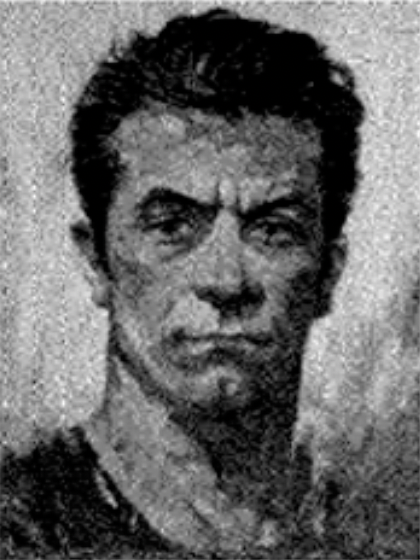
\includegraphics[width=0.21\linewidth]{figures/chapter4/fig5-a.png}}
  \quad\quad\quad\quad\quad
  \subfigure[使用AES在ECB模式下加密明文]{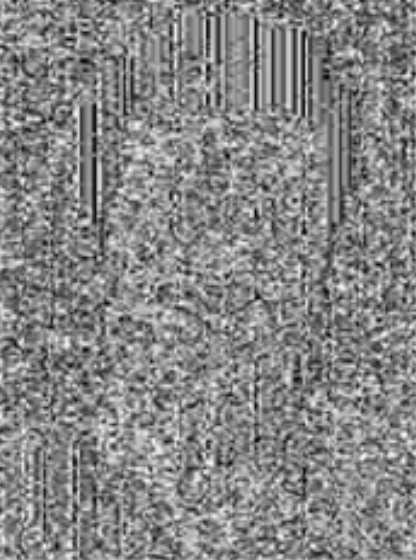
\includegraphics[width=0.21\linewidth]{figures/chapter4/fig5-b.png}}
  \caption{ECB模式中的加密}
  \label{fig:4-5}
\end{figure}

\begin{theorem}\label{theo:4-1}
令 $\mathcal{E}=(E,D)$ 是一个分组密码,$\ell\geq1$ 是任意多项式边界的值,令 $\mathcal{E}'=(E',D')$ 是由 $\mathcal{E}$ 派生的 $\ell$ 次 ECB 密码,但其消息空间被限制为最多 $\ell$ 个各不相同的数据分组的所有可能序列。如果 $\mathcal{E}$ 是一个安全的分组密码,那么 $\mathcal{E}'$ 就是一个语义安全的密码。
\begin{quote}
特别地,对于每个就 $\mathcal{E}'$ 进行攻击游戏 \ref{game:2-1} 的 SS 对手 $\mathcal{A}$,都存在一个就 $\mathcal{E}$ 进行攻击游戏 \ref{game:4-1} 的 BC 对手 $\mathcal{B}$,其中 $\mathcal{B}$ 是一个围绕 $\mathcal{A}$ 的基本包装器,满足:
\end{quote}
\begin{equation}\label{eq:4-3}
{\rm SS\mathsf{adv}}[\mathcal{A},\mathcal{E}']=2\cdot{\rm BC\mathsf{adv}}[\mathcal{B},\mathcal{E}]
\end{equation}
\end{theorem}

\begin{proof}[证明思路]
基本思想是,如果对手被赋予了一条消息的加密,而该消息是一串各不相同的数据分组,那么对手能看到的实际上也只是一个随机数据分组的序列(无替换采样)。
\end{proof}

\begin{proof}
如果 $\mathcal{E}$ 定义在 $(\mathcal{K},\mathcal{X})$ 上,令 $\mathcal{X}_*^{\leq\ell}$ 表示 $\mathcal{X}$ 中由最多 $\ell$ 个不同元素所组成的所有序列的集合。

令 $\mathcal{A}$ 是一个有效对手,它像攻击游戏 \ref{game:2-1} 中那样攻击 $\mathcal{E}'$。我们的目标是,假设 $\mathcal{E}$ 是一个安全的分组密码,证明 ${\rm SS\mathsf{adv}}[\mathcal{A},\mathcal{E}']$ 是可忽略不计的。使用语义安全攻击游戏的比特猜测版本更加方便。我们试图证明:
\begin{equation}\label{eq:4-4}
{\rm SS\mathsf{adv}}^*[\mathcal{A},\mathcal{E}']={\rm BC\mathsf{adv}}[\mathcal{B},\mathcal{E}]
\end{equation}
对于某个有效对手 $\mathcal{B}$ 成立。那么根据定理 \ref{theo:2-10},我们就能得到式 \ref{eq:4-3}。

所以,考虑对手 $\mathcal{A}$ 在攻击游戏 \ref{game:2-1} 的比特猜测版本中对 $\mathcal{E}'$ 的攻击。在这个游戏中,$\mathcal{A}$ 向挑战者发送两条长度相同的消息 $m_0,m_1$,然后挑战者选择一个随机密钥 $k$ 和一个随机比特 $b$,并用 $k$ 加密 $m_b$,将得到的密文 $c$ 交给 $\mathcal{A}$;最后,$\mathcal{A}$ 输出一个比特 $\hat b$。如果 $\hat b=b$,则对手 $\mathcal{A}$ 赢得游戏。

挑战者在该游戏中的逻辑可以表示如下:

\vspace*{10pt}

\hspace*{5pt} 当从对手 $\mathcal{A}$ 处收到消息 $m_0,m_1\in\mathcal{X}_*^{\leq\ell}$ 时,记 $v:=|m_0|=|m_1|$:\\
\hspace*{50pt} 选取 $b\overset{\rm R}\leftarrow\{0,1\}$\\
\hspace*{50pt} 选取 $k\overset{\rm R}\leftarrow\mathcal{K}$\\
\hspace*{50pt} 令 $c\leftarrow(E(k,m_b[0]),\dots,E(k, m_b[v-1]))$\\
\hspace*{50pt} 将 $c$ 发送给 $\mathcal{A}$。

\vspace*{10pt}

我们将该游戏称作\textbf{游戏 $\mathbf{0}$}。我们下面还将定义游戏 $1$ 和游戏 $2$。对于 $j=0,1,2$,我们定义 $W_j$ 为 $\mathcal{A}$ 在游戏 $j$ 中输出的 $\hat b=b$ 的事件。根据定义,我们有:
\begin{equation}\label{eq:4-5}
\mathrm{SS}\mathsf{adv}^*[\mathcal{A},\mathcal{E}']
=
|\Pr[W_0]-{1}/{2}|
\end{equation}

\noindent
\textbf{游戏 $\mathbf{1}$}。该游戏与游戏 $0$ 基本相同,只是现在,挑战者用一个随机的 $f\in{\rm Perms}[\mathcal{X}]$ 代替 $E(k,\cdot)$。我们的挑战者现在看起来是这样的:

\vspace*{10pt}

\hspace*{5pt} 当从对手 $\mathcal{A}$ 处收到消息 $m_0,m_1\in\mathcal{X}_*^{\leq\ell}$ 时,记 $v:=|m_0|=|m_1|$:\\
\hspace*{50pt} 选取 $b\overset{\rm R}\leftarrow\{0,1\}$\\
\hspace*{50pt} 选取 $f\overset{\rm R}\leftarrow{\rm Perms}[\mathcal{X}]$\\
\hspace*{50pt} 令 $c\leftarrow(f(m_b[0]),\dots,f(m_b[v-1]))$\\
\hspace*{50pt} 将 $c$ 发送给 $\mathcal{A}$。

\vspace*{10pt}

直观地说,$\mathcal{E}$ 是一个安全的分组密码的事实意味着,对手应该注意不到这个变化。为了严格地证明这一点,我们下面展示,如何构建一个分组密码对手 $\mathcal{B}$,使得它是一个围绕 $\mathcal{A}$ 的基本包装器,且满足:
\begin{equation}\label{eq:4-6}
\big\lvert
\Pr[W_0]-\Pr[W_1]
\big\rvert
=\mathrm{BC}\mathsf{adv}[\mathcal{B},\mathcal{E}]
\end{equation}

$\mathcal{B}$ 的设计直接来自于游戏 $0$ 和 $1$ 的逻辑。对手 $\mathcal{B}$ 就 $\mathcal{E}$ 进行攻击游戏 \ref{game:4-1},其工作原理如下:
\begin{quote}
记 $f$ 为 $\mathcal{B}$ 的分组密码挑战者在攻击游戏 \ref{game:4-1} 中选择的函数。我们让 $\mathcal{B}$ 扮演 $\mathcal{A}$ 的挑战者的角色,其工作逻辑如下:

\vspace*{5pt}

\hspace*{20pt} 当从对手 $\mathcal{A}$ 处收到消息 $m_0,m_1\in\mathcal{X}_*^{\leq\ell}$ 时,记 $v:=|m_0|=|m_1|$:\\
\hspace*{50pt} 选取 $b\overset{\rm R}\leftarrow\{0,1\}$\\
\hspace*{50pt} 令 $c\leftarrow(f(m_b[0]),\dots,f(m_b[v-1]))$\\
\hspace*{50pt} 将 $c$ 发送给 $\mathcal{A}$。

\vspace*{5pt}

请注意,$\mathcal{B}$ 通过查询它自己的分组密码挑战者来计算 $f(m_b[0]),\dots,f(m_b[v-1])$。最后,当 $\mathcal{A}$ 输出一个比特 $\hat b$ 时,$\mathcal{B}$ 输出 $\delta(\hat b,b)$,其中 $\delta$ 的定义见式 \ref{eq:3-7}。
\end{quote}

\vspace{8pt}

\noindent
显然,当 $\mathcal{B}$ 处于其攻击游戏的实验 $0$ 时,它会以 $\Pr[W_0]$ 的概率输出 $1$。而当 $\mathcal{B}$ 处于其攻击游戏的实验 $1$ 时,它会以 $\Pr[W_1]$ 的概率输出 $1$。这样,我们就能得到式 \ref{eq:4-6}。

\vspace{8pt}

\noindent
\textbf{游戏 $\mathbf{2}$}。
现在,我们重写游戏 $1$ 中的挑战者,让其使用我们在 \ref{subsec:4-1-2} 小节中讨论的``忠实的侏儒"来实现随机置换。$m_0$ 和 $m_1$ 的每条消息都需要由各不相同的数据分组组成(我们的挑战者不需要验证这一点),因此我们的侏儒的工作很容易:它甚至不需要看输入数据分组,因为这些数据分组被确保是各不相同的;然而,它仍然需要确保它产生的输出分组是各不相同的。

我们可以把我们的挑战者的逻辑表述如下:

\vspace*{10pt}

\hspace*{5pt} 选取 $y_0\overset{\rm R}\leftarrow\mathcal{X}$,$y_1\overset{\rm R}\leftarrow\mathcal{X}\setminus\{y_0\}$,$\dots$,$y_{\ell-1}\overset{\rm R}\leftarrow\mathcal{X}\setminus\{y_0,\dots,y_{\ell-2}\}$\\
\hspace*{26pt} 当从对手 $\mathcal{A}$ 处收到消息 $m_0,m_1\in\mathcal{X}_*^{\leq\ell}$ 时,记 $v:=|m_0|=|m_1|$:\\
\hspace*{50pt} 选取 $b\overset{\rm R}\leftarrow\{0,1\}$\\
\hspace*{50pt} 令 $c\leftarrow(y_0,\dots,y_{v-1})$\\
\hspace*{50pt} 将 $c$ 发送给 $\mathcal{A}$。

\vspace*{10pt}

由于我们的侏儒是忠实的,我们有:
\begin{equation}\label{eq:4-7}
\Pr[W_1]=\Pr[W_2]
\end{equation}
此外,我们声称:
\begin{equation}\label{eq:4-8}
\Pr[W_2]={1}/{2}
\end{equation}
这来自这样一个事实:在游戏 $2$ 中,对手的输出 $\hat b$ 是它自己的随机选择,以及 $y_0,\dots,y_{\ell-1}$ 的一个函数。由于这些值(根据定义)与 $b$ 无关,因此 $\hat b$ 和 $b$ 是相互独立的。所以式 \ref{eq:4-8} 成立。

综合式 \ref{eq:4-5},式 \ref{eq:4-6},式 \ref{eq:4-7} 和式 \ref{eq:4-8},我们就能得到式 \ref{eq:4-4},因此定理 \ref{theo:4-1} 得证。
\end{proof}

\subsection{数学细节}\label{subsec:4-1-5}

和之前一样,我们下面讨论一些之前被忽略了的数学细节。

由于分组密码只是一种特殊的密码,所以关于分组密码的定义,其实没有什么是 \ref{sec:2-3} 节中没有交代的。像往常一样,定义 \ref{def:4-1} 需要被正确地解释。首先,在攻击游戏 \ref{game:4-1} 中,我们要理解,对于安全参数 $\lambda$ 的每个值,我们都会得到一个不同的概率空间,它由挑战者的随机选择和对手的随机选择共同决定。其次,挑战者会产生一个系统参数 $\Lambda$,并在游戏一开始就将其发送给对手。第三,优势 ${\rm BC\mathsf{adv}}[\mathcal{B},\mathcal{E}]$ 是安全参数 $\lambda$ 的一个函数,安全性则意味着它是一个可忽略不计函数。
\section{在实践中构建分组密码}\label{sec:4-2}

分组密码是密码学中的一个基本原语,许多其他系统都是基于它建立的。几乎所有在实践中使用的分组密码都使用了相同的基本框架,称为\textbf{迭代密码 (iterated cipher)}范式。为了构建一个迭代分组密码,设计者需要做出以下两个抉择:
\begin{itemize}
	\item 首先,他需要选择一个简单的分组密码 $\mathcal{\hat E}:=(\hat E,\hat D)$,它本身显然是不安全的。我们称 $\mathcal{\hat E}$ 为\textbf{轮密码 (round cipher)}。
	\item 其次,他还需要选择一个简单(但不一定安全)的 PRG $G$,用来将密钥 $k$ 扩展为 $\mathcal{\hat E}$ 的 $d$ 个密钥 $k_1,\dots,k_d$。我们称 $G$ 为\textbf{密钥扩展函数 (key expansion function)}。
\end{itemize}
一旦做出这两个选择,迭代分组密码 $\mathcal{E}$ 就完全确定下来了。加密算法 $E(k,x)$ 的工作原理如下(另见图 \ref{fig:4-6}):

\begin{figure}
  \centering
  \input{figures/chapter4/fig6.tex}
  \caption{现实世界中分组密码的加密}
  \label{fig:4-6}
\end{figure}

\begin{quote}
\begin{quote}
\begin{quote}
\begin{tcolorbox}[colframe=black,colback=white,boxrule=0.6pt,arc=0pt]
算法$E(k,x)$:

\vspace{5pt}

\begin{enumerate}
	\item \textbf{密钥扩展}:使用密钥扩展函数 $G$ 将 $\mathcal{E}$ 的密钥 $k$ 扩展为 $\mathcal{\hat E}$ 的 $d$ 个密钥:
	\[(k_1,\dots,k_d)\leftarrow G(k)\]
    \item \textbf{迭代}:对于 $i=1,2,\dots,d$,计算 $\hat E(k_i,\cdot)$,即:
    \[y\leftarrow\hat{E}(k_d,\;\hat{E}(k_{d-1},\dots,\hat{E}(k_2,\;\hat{E}(k_1,\;x))\dots))\]
\end{enumerate}
\end{tcolorbox}
\end{quote}
\end{quote}
\end{quote}
$\mathcal{\hat E}$ 的每次应用都被称为一\textbf{轮 (round)},总轮数为 $d$。$k_1,\dots,k_d$ 被称为\textbf{轮密钥 (round keys)}。解密算法 $D(k, y)$ 与加密算法 $E(k,x)$ 基本相同,除了在解密时,轮密钥是被反向使用的。$D(k,y)$ 的定义如下:
\[
x\leftarrow\hat{D}(k_1,\hat{D}(k_2,\dots,\hat{D}(k_{d-1},\hat{D}(k_d,y))\dots))
\]
表 \ref{tab:4-1} 列出了一些常见的分组密码和它们的相关参数。我们将在下一节中介绍 DES 和 AES。

\begin{snote}[迭代是否能提供安全的分组密码?]
没有人知道。然而,启发式的证据表明,分组密码的安全性来自于对简单密码的多次迭代。但并非所有的轮密码都能发挥作用。例如,无论迭代多少次,下面这样的线性函数:
\[
\hat E(k,x)=k\cdot x\bmod q
\]
都无法产生一个安全的分组密码,因为对 $\hat E$ 的迭代只会产生另一个线性函数。目前还没有办法辨别哪些轮密码最终能产生安全的分组密码。此外,对于一个候选的轮密码 $\hat E$,我们也还没有严格的方法来衡量需要迭代它多少次才能生成一个安全的分组密码。我们知道的是,某些函数,比如线性函数,是完全不可能导出安全分组密码的。但是简单的非线性函数似乎在几次迭代后就能得到一个安全的分组密码。

密码学家面临的挑战是要想出一个快速的轮密码,它在几轮之内就能收敛为一个安全分组密码。看看表 \ref{tab:4-1},以 AES-128 为例,它使用了一个很简单的轮密码,但只需要十轮迭代就能产生一个安全的分组密码,这种卓越的性能表现令人印象深刻。
\end{snote}

\begin{table}
\centering
\begin{tabular}{lcccc}
\hline
 &
  \begin{tabular}[c]{@{}c@{}}key size\\ (bits)\end{tabular} &
  \begin{tabular}[c]{@{}c@{}}block size\\ (bits)\end{tabular} &
  \begin{tabular}[c]{@{}c@{}}number of\\ rounds\end{tabular} &
  \begin{tabular}[c]{@{}c@{}}performance\footnotemark[1]\\ (MB/s)\end{tabular} \\ \hline
DES     & 56  & 64  & 16 & 80  \\
3DES    & 168 & 64  & 48 & 30  \\
AES-128 & 128 & 128 & 10 & 163 \\
AES-256 & 256 & 128 & 14 & 115 \\ \hline
\end{tabular}
\caption{分组密码示例}
\label{tab:4-1}
\end{table}

\footnotetext[1]{性能数字是使用 OpenSSL 1.0.1e 在 Intel(R) Xeon(R) CPU E5-2698 v3 @ 2.30GHz (Haswell) 处理器上运行获得的。}

\begin{snote}[注意事项。]
虽然本节将要解释几种分组密码的内部工作原理,但它并不会教授如何设计新的分组密码。事实上,本节的主要收获之一是,读者不应自行设计分组密码,而应该始终使用这里描述的标准密码。分组密码的设计非同小可,需要经过多年的分析才能对某一具体方案产生充分信心。此外,读者甚至不应该自己实现分组密码,因为分组密码的实现往往容易受到计时攻击和功耗攻击,就如 \ref{subsec:4-3-2} 小节将要讨论的。使用诸如 OpenSSL 等密码库中免费提供的标准实现要安全得多。这些实现经历了多年来的反复分析,并已被多次加固以抵御各种攻击。
\end{snote}

\subsection{案例研究:DES}\label{subsec:4-2-1}

上世纪 70 年代,美国国家标准局 (National Bureau of Standards, NBS),即现在的美国国家标准技术研究所 (National Institute of Standards and Technology, NIST) 向社会公开征集加密方案。因应这一需求,IBM 开发了数据加密标准 (Data Encryption Standard, DES)。它于 1975 年在联邦公报上发表,并于 1977 年被采纳为``非机密"应用的加密标准。DES 算法单枪匹马地开启了密码分析领域,因为所有人都想破解它。自诞生以来,DES 经历了相当多的分析,也间接导致了许多分组密码分析工具的出现。

DES 的前身是 IBM 早期设计的一个分组密码,名为 Lucifer。Lucifer 的某些变体使用 $128$ 比特密钥对 $128$ 比特的分组进行操作。然而,国家标准局要求设计使用更短分组($64$ 比特)和更短密钥($56$ 比特)的分组密码。作为回应,IBM 团队设计了一个符合这些要求的密码,并在最终成为了 DES。将 DES 的密钥大小设定为 $56$ 比特在当时饱受批评。甚至有人猜测 DES 的这种弱设计是美国情报机构故意要求的。在接下来的章节中,我们还会看到将分组大小减少到 $64$ 比特也带来了许多问题。

由于密钥太短,DES 算法现在被认为是不安全的,不应该再被使用。然而,一个名为 Triple-DES (3DES) 的加强版 DES 在 1998 年被重新确立为美国国家标准。NIST 已经批准 3DES 供政府使用,直至 2030 年。在 2002 年,DES 被一个更高效的分组密码标准所取代,后者就是 AES,它使用 $128$ 比特(或更长)的密钥,并在 $128$ 比特的分组上运行。

\subsubsection{DES 算法}\label{subsubsec:4-2-1-1}

DES 算法由一个简单的轮密码经 $16$ 次迭代组成。为了描述 DES,我们需要先介绍 DES 的轮密码和密钥扩展函数。我们下面依次介绍它们。

\begin{snote}[Feistel 置换法。]
DES 的关键创新之一是由 IBM 的 Horst Feistel 发明的 Feistel 置换法 (Feistel Permutation),它能基于任意函数建立一个置换。令 $f:\mathcal{X}\to\mathcal{X}$ 是一个函数,我们按如下方法构建一个置换 $\pi:\mathcal{X}^2\to\mathcal{X}^2$(见图 \ref{fig:4-7}):
\[
\pi(x,y)
:=
\big(
y,\;x\oplus f(y)
\big)
\]
为了证明 $\pi$ 是一个双射,我们给出它的逆变换:
\[
\pi^{-1}(u,v)
=
\big(
v\oplus f(u),\;u
\big)
\]
映射 $\pi$ 被称为\textbf{Feistel 置换},它被用于构建 DES 轮密码。$n$ 个 Feistel 置换的组合被称为 \textbf{$n$ 轮 Feistel 网络 ($n$-round Feistel network)}。设计成 Feistel 网络的分组密码被称为\textbf{Feistel 密码}。对于 DES 来说,函数 $f$ 需要 $32$ 比特输入,产生的映射 $\pi$ 对 $64$ 比特的分组进行操作。

需要注意的是,Feistel 逆置换 $\pi^{-1}$ 几乎与 $\pi$ 完全相同。因此,我们只用设计一套硬件电路,就能同时计算 $\pi^{-1}$ 和 $\pi$。这也意味着加密和解密电路也可以使用相同的硬件实现。
\end{snote}

\begin{figure}
  \centering
  \input{figures/chapter4/fig7.tex}
  \caption{Feistel 置换法}
  \label{fig:4-7}
\end{figure}

\begin{figure}[p!]
  \centering
  \input{figures/chapter4/fig8.tex}
  \caption{DES的轮函数$F(k,x)$}
  \label{fig:4-8}
\end{figure}

\begin{snote}[DES 轮函数。]
DES 加密算法是一个 $16$ 轮 Feistel 网络,每轮使用一个不同的函数 $f:\mathcal{X}\to\mathcal{X}$。在第 $i$ 轮中,函数 $f$ 的定义为:
\[
f(x):=F(k_i,x)
\]
其中,$k_i$ 是第 $i$ 轮的 $48$ 比特密钥,$F$ 是一个固定函数,称为 \textbf{DES 轮函数}。函数 $F$ 是 DES 算法的核心,如图 \ref{fig:4-8} 所示。$F$ 使用的几个辅助函数 $E$、$P$ 和 $S_1,\dots,S_8$ 定义如下:
\begin{itemize}
	\item 函数 $E$ 通过对输入比特的重新排列和复制,将 $32$ 比特输入扩展为 $48$ 比特输出。例如,$E$ 将输入的第 $1$ 比特映射到输出的第 $2$ 和第 $48$ 比特,将输入的第 $2$ 比特映射到输出的第 $3$ 比特,以此类推。
	\item 函数 $P$ 称为\textbf{混合置换 (mixing permutation)},它通过重新排列输入的比特,将 $32$ 比特输入映射到 $32$ 比特输出。例如,$P$ 将输入的第 $1$ 比特映射到输出的第 $9$ 比特,将输入的第 $2$ 比特映射到输出的第 $15$ 比特,以此类推。
	\item 函数 $S_1,\dots,S_8$ 称为 \textbf{S 盒 (S-boxes)}。每个 S 盒 $S_i$ 通过一张查找表将一个 $6$ 比特输入映射为一个 $4$ 比特输出。DES 标准列出了这 $8$ 张查找表,每张表中包含 $64$ 项。
\end{itemize}

\noindent
基于以上函数,DES 的轮函数 $F(k,x)$ 工作原理如下:

\vspace*{10pt}

\hspace*{5pt} 输入:$k\in\{0,1\}^{48}$ 和 $x\in\{0,1\}^{32}$\\
\hspace*{26pt} 输出:$y\in\{0,1\}^{32}$

\vspace*{5pt}

\hspace*{5pt} $F(k,x)$:\\
\hspace*{50pt} 计算 $t\leftarrow E(x)\oplus k\quad\in\{0,1\}^{48}$\\
\hspace*{50pt} 将 $t$ 分成 $8$ 组,每组 $6$ 比特:$t:=t_1\,\Vert\,\cdots\,\Vert\,t_8$\\
\hspace*{50pt} 对于 $i=1,2,\dots,8$,令 $s_i\leftarrow S_i(t_i)$\\
\hspace*{50pt} 组合 $s\leftarrow s_1\,\Vert\,\cdots\,\Vert\,s_8\quad\in\{0,1\}^{32}$\\
\hspace*{50pt} 计算 $y\leftarrow P(s)\quad\in\{0,1\}^{32}$\\
\hspace*{50pt} 输出 $y$

\vspace*{10pt}

\noindent
除了 S 盒,DES 的轮密码完全由异或操作和比特置换组成。八个 S 盒是设计中唯一引入的非线性组件。在公开文献揭示了一种名为``差分密码分析"的强大攻击技术后,IBM 于 1994 年公布了 S 盒的设计标准 \cite{coppersmith1994data}。IBM 的这份报告清楚地表明,DES 的设计者早在 1973 年就已经了解了多年后才在公开文献中出现的这种攻击技术。他们在设计 DES 时加入了抵抗这种攻击的因素。下面这段话解释了对 S 盒设计标准保密的原因 \cite{coppersmith1994data}:
\begin{quote}
我们在设计 DES 时利用了某些密码分析技术的知识,其中最突出的是``差分密码分析"技术,这些技术在公开的文献中并不为人所知。在与美国国家安全局讨论后,我们认为,设计思路一经披露,就会反过来揭示这种差分密码分析技术。这种技术非常强大,可以用来对付很多密码器,因此会削弱美国在密码学领域相对其他国家的竞争优势。
\end{quote}
一旦差分密码分析技术被公开,再保密 DES 的设计思路也就没有太多意义了。考虑到 S 盒的重要性,我们下面列举了当初设计它的一些准则,正如 \cite{coppersmith1994data} 中所解释的那样:
\begin{enumerate}
	\item 查找表的大小,即将 $6$ 比特输入映射为 $4$ 比特输出,是以 1974 年的技术能在单个芯片上做到的最大尺寸。
	\item S 盒的任何输出比特都不应该接近于输入比特的某个线性函数。也就是说,如果我们选择任何一个输出比特和 $6$ 个输入比特的任何一个子集,这个输出比特等于这些输入比特的异或结果的概率都应该接近 $1/2$。
	\item 如果我们把输入的最左边和最右边的比特固定在一个 S 盒上,那么产生的 $4$ 比特到 $4$ 比特的函数是一个双射。特别地,这意味着每个 S 盒都是一个 $4$ 到 $1$ 的映射。
	\item 改变 S 盒的一个输入比特,至少会导致两个输出比特被改变。
	\item 对于每个 $\Delta\in\{0,1\}^6$,在满足 $x\oplus y=\Delta$ 的 $64$ 对 $x,y\in\{0,1\}^6$ 中,$S_i(x)\oplus S_i(y)$ 计算得到同一个值的情况不得超过 $8$ 次。
\end{enumerate}
这些标准是为了让 DES 尽可能地强大,尽管限制它的密钥只能有 $56$ 比特长。现在我们已经知道,如果 S 盒是简单随机选出的,产生的 DES 密码有很大概率是不安全的。特别是,对手可能只需要对挑战者进行几百万次查询,就可以恢复出秘钥。

除了 S 盒之外,混合置换 $P$ 也起着重要的作用。它确保 S 盒不总是在同一组 $6$ 比特上进行操作。同样,\cite{coppersmith1994data} 也列出了选择置换 $P$ 的一系列标准。如果 $P$ 是简单随机选出的,DES 的安全性也将大打折扣。

\end{snote}

\begin{figure}
  \centering
  \input{figures/chapter4/fig9.tex}
  \caption{完整的DES电路}
  \label{fig:4-9}
\end{figure}

\begin{snote}[密钥扩展函数。]
DES 的密钥扩展函数 $G$ 将 $56$ 比特的密钥 $k$ 作为输入,输出 $16$ 个密钥 $k_1,\dots,k_{16}$,每个 $48$ 比特长。每个密钥 $k_i$ 都由从 $56$ 比特密钥 $k$ 中选出的 $48$ 个比特组成,每个 $k_i$ 都使用 $k$ 中比特的不同子集。
\end{snote}

\begin{snote}[DES 算法。]
完整的 DES 算法架构如图 \ref{fig:4-9} 所示,它包括对 DES 轮密码的 $16$ 次迭代,以及被称为 IP 和 FP 的初始和最后的置换。这些置换只是重新排列了 $64$ 比特的输入和输出,其中,FP 置换是 IP 置换的逆变换。

IP 和 FP 没有任何密码学意义,被包括在算法内的原因至今不明。由于比特置换在软件实现中很慢,但在硬件实现中却很快,一种理论认为,IP 和 FP 是为了故意减慢 DES 的软件实现才被加入的。
\end{snote}

\subsection{对 DES 的穷举搜索:DES 挑战}\label{subsec:4-2-2}

回顾一下,对分组密码 $(E,D)$ 的穷举搜索攻击(\ref{subsubsec:4-1-1-2} 小节)指的是这样的攻击:给予对手少量的明文分组 $x_1,\dots,x_Q\in\mathcal{X}$ 和使用 $\mathcal{K}$ 中的密钥 $k$ 加密它们得到的密文分组 $y_1,\dots,y_Q$。对手尝试所有可能的 $\mathpzc{k}\in\mathcal{K}$,直至找到一个密钥 $k$,能够将所有给定的明文分组映射到给定的密文分组上。如果给定的密文分组足够多,$k$ 就是唯一能够实现这种映射的密钥,而且它终将被对手发现。

对于像 DES 和 AES-128 这样的分组密码,仅需\emph{三}个分组就足以确保有唯一密钥能以较大概率将给定的明文分组映射到给定的密文分组。我们将在 \ref{subsec:4-7-2} 小节讨论理想密码及其特性时看到原因。现在我们只需知道,给定三个明文/密文分组对,攻击者就可以用穷举法找到秘钥 $k$。

在 1974 年设计 DES 时,对大小为 $2^{56}$ 的密钥空间进行穷举搜索攻击被认为是不可行的。但随着计算机硬件的持续发展,人们渐渐发现 $56$ 比特的密钥远远不够。

为了证明对 DES 的穷举搜索是可行的,RSA 数据安全部设置了一连串的挑战,称为 \textbf{DES 挑战}。规则很简单:在一个预先宣布的日期,RSA 数据安全部将会公布三个 DES 输入/输出对。第一个找到相应密钥的小组就能赢得一万美元。为了使挑战更具娱乐性,挑战包含 $n$ 个 DES 输出 $y_1,y_2,\dots,y_n$,其中的前三个输出 $y_1,y_2,y_3$ 是对下面这 $24$ 字节明文消息应用 DES 后得到的结果:
\begin{figure*}[h!]
  \centering
  \input{figures/chapter4/vac1.tex}
\end{figure*}

\noindent
该消息由 $3$ 个 DES 分组构成,每个分组为 $8$ 字节,也就是 $64$ 比特。目标是找到一个 DES 密钥,对于 $i=1,2,3$,该密钥能够将 $x_i$ 映射到 $y_i$。得到密钥后,挑战者就能够使用密钥来解密 $y_4,\dots,y_n$ 编码的秘密消息。

第一个挑战在 1997 年 1 月发布。\textsc{deschall} 项目组用 $96$ 天的时间解决了它。该团队在 $78,000$ 名志愿者的帮助下使用众包搜索的方式进行破解,这些志愿者贡献了他们自己设备的闲置算力。找到秘钥的志愿者获得了 $40\%$ 的奖金。解密后大家得知,$y_4,\dots,y_n$ 对应的明文是``强大的密码学使世界更加安全。" (Strong cryptography makes the world a safer place.)

第二个挑战于 1998 年 1 月发布。\textbf{distributed.net} 项目组使用了类似的但规模更大的众包搜索,仅用时 41 天就解决了该挑战。

1998 年初,电子前沿基金会 (Electronic Frontiers Foundation, EFF) 与 Paul Kocher 签订合同,建造一台专门的设备来进行针对 DES 的穷举密钥搜索。这台机器被称为\textbf{DeepCrack},耗资 25 万美元,包含大约 1900 个专用 DES 芯片,装在六个柜子里。这些芯片并行工作,每个芯片在指定的密钥空间中搜索。当 RSA 数据安全部在 1998 年 7 月发布下一个挑战时,DeepCrack 在 56 小时内就解决了这个挑战,并轻松赢得了一万美元的奖金。这还不足以支付机器的成本,但足以说明 DES 存在致命问题。

最后的挑战是在 1999 年 1 月发布的。在 DeepCrack 和 \emph{distributed.net} 的共同努力下,它在 22 小时内就被破解了。这在 DES 的棺材板上钉上了最后一颗钉子,表明 $56$ 比特的密钥可以在短短几个小时内就被破解。

在这个故事的末尾,2007 年,\textsc{copacobana} 团队建立了一个由现成的 120 块 FPGA 板组成的集群,总成本约为 1 万美元。该集群可以在大约 12.8 天内搜索完整个 $2^{56}$ 的 DES 密钥空间 \cite{guneysu2008cryptanalysis}。

上述所有工作将我们导向一个共同的结论,那就是 $56$ 比特密钥实在太短了。目前的最小安全密钥长度是 $128$ 比特。

\subsubsection{穷举搜索对 AES-128 是否奏效?}\label{subsubsec:4-2-2-1}

让我们把 DES 上的结论推广到 AES。虽然这些估计本身是不精确的,但它们在一定程度上说明了针对 AES 的穷举搜索的复杂性。AES 的密钥空间最小是 $2^{128}$。如果扫描一个 $2^{56}$ 的空间需要 22 小时,那么扫描一个 $2^{128}$ 大小的空间将需要:
\[
(22\;{\rm hours})\times2^{128-56}\approx1.18\times10^{20}\;{\rm years}
\]
即使计算速度和计算资源能提升十亿倍,即使 AES 计算比 DES 计算更快,所需的时间也远超人类的认知范围。因此,我们可以得出这样的结论:对 AES 进行暴力穷举式的搜索攻击是不现实的。然而,正如我们将在 \ref{sec:18-7} 节中讨论的,如果利用时空权衡这一经典思路,我们仍然可以对 AES-128 发起更复杂的暴力攻击。

\subsection{加强密码以抵抗穷举攻击:$3\mathcal{E}$构造}\label{subsec:4-2-3}

事实证明,DES 密码对复杂的攻击有很强的抵抗力。尽管经过了多年的分析,对 DES 最实用的攻击仍然是对整个密钥空间进行暴力穷举搜索。唯一的问题就是,$56$ 比特的密钥空间太小了。

一个自然而然的想法是,我们能否在不改变其内部结构的情况下加强密码的抗穷举攻击能力?最简单的解决方案是使用独立的密钥对密码进行多次迭代。

令 $\mathcal{E}=(E,D)$ 是一个定义在 $(\mathcal{K},\mathcal{X})$ 上的分组密码。我们定义分组密码 $3\mathcal{E}=(E_3,D_3)$ 为:
\[
E_3\big((k_1,k_2,k_3),\;x\big)
:=
E\big(k_3,\;E(k_2,\;E(k_1,x))\big)
\]
$3\mathcal{E}$ 密码的密钥在 $\mathcal{K}^3$ 上。基于 DES 算法的 $3\mathcal{E}$ 密码被称为 \textbf{Triple-DES},它的密钥长度为 $3\times56=168$ 比特。

\begin{snote}[安全性。]
为了分析 $3\mathcal{E}$ 密码的安全性,我们需要一个称为\emph{理想密码模型}的框架。我们将在本章末尾介绍这个框架,并在那一节中分析 $3\mathcal{E}$ 密码的安全性。
\end{snote}

\begin{snote}[Triple-DES 标准。]
NIST 批准 Triple-DES 在 2030 年前可以供政府使用。严格来说,NIST 版本的 Triple-DES 的定义为:
\[
E_3\big((k_1,k_2,k_3),\;x\big)
:=
E\big(k_3,\;D(k_2,\;E(k_1,x))\big)
\]
其原因是,如果设置 $k_1=k_2=k_3$,NIST 的 Triple-DES 就可以被还原为普通 DES,因此 Triple-DES 的硬件实现也可以直接复用于单一 DES 的场景中。这个修改不会影响我们对 Triple-DES 安全性的讨论。练习 \ref{exer:4-5} 中还讨论了 Triple-DES 的另一个变体。
\end{snote}

\subsubsection{$2\mathcal{E}$ 构造是不安全的}

虽然 Triple-DES 不容易被穷举搜索攻击所攻破,但它的性能比单一 DES 慢三倍,如表 \ref{tab:4-1} 所示。

那么为什么不使用 Double-DES 呢?它的密钥长度是 $2\times56=112$ 比特,这已经足以抵抗穷举搜索,而且它的性能也要比 Triple-DES 好得多。

问题在于,Double-DES 并不比单一 DES 更安全。更一般地说,令 $\mathcal{E}=(E,D)$ 是一个具有密钥空间 $\mathcal{K}$ 的分组密码。我们能够证明,定义为:
\[
E_2\big((k_1,k_2),\;x\big)
:=
E\big(k_2,\;E(k_1,x)\big)
\]
的 $2\mathcal{E}=(E_2,D_2)$ 构造不会比 $\mathcal{E}$ 更安全。针对它的攻击策略被称为\textbf{中间相遇 (meet in the middle)}。

假设我们得到了 $Q$ 个明文分组 $x_1,\dots,x_Q$,以及它们的 $2\mathcal{E}$ 加密 $y_i=E_2\big((k_1,k_2),x_i\big)$,其中 $i=1,\dots,Q$。我们下面展示如何在正比于 $|\mathcal{K}|$ 的时间内恢复密钥 $(k_1,k_2)$,即使密钥空间的大小为 $|\mathcal{K}|^2$。和单一 DES 的穷举搜索一样,我们只需少量的明文/密文对,就足以确保以高概率恢复唯一的密钥 $(k_1,k_2)$。事实上,对于像 Double-DES 这样的分组密码来说,$10$ 个分组就足以确保密钥的唯一性了。

\begin{theorem}\label{theo:4-2}
令 $\mathcal{E}=(E,D)$ 是一个定义在 $(\mathcal{K},\mathcal{X})$ 上的分组密码。存在一种算法 $\mathcal{A}_{{\rm E}X}$,它以 $Q$ 个明文/密文对 $(x_i,y_i)\in\mathcal{X}^2$作为输入,其中 $i=1,\dots,Q$,输出一个密钥对 $(\mathpzc{k}_1,\mathpzc{k}_2)\in\mathcal{K}^2$,满足:
\begin{equation}\label{eq:4-9}
y_i=E_2\big((\mathpzc{k}_1,\mathpzc{k}_2),\;x_i\big)
\quad\text{ for all }
i=1,\dots,Q
\end{equation}
其运行时间的主要成分是对算法 $E$ 和算法 $D$ 的总计 $2Q\cdot|\mathcal{K}|$ 次评估的耗时。
\end{theorem}

\begin{figure}
  \centering
  \input{figures/chapter4/fig10.tex}
  \caption{$2\mathcal{E}$上的中间相遇攻击}
  \label{fig:4-10}
\end{figure}

\begin{proof}
令 $\bar{x}:=(x_1,\dots,x_Q)$,$\bar{y}:=(y_1,\dots,y_Q)$。为了简化符号,我们用:
\[
\bar y=E_2\big((\mathpzc{k}_1,\mathpzc{k}_2),\;\bar x)=E(\mathpzc{k}_2,\;E(\mathpzc{k}_1,\bar x)\big)
\]
来描述式 \ref{eq:4-9} 中的 $Q$ 个映射。我们也可以把它写成:
\begin{equation}\label{eq:4-10}
D(\mathpzc{k}_2,\bar y)=E(\mathpzc{k}_1,\bar x)
\end{equation}
为了找到能满足式 \ref{eq:4-10} 的一对 $(\mathpzc{k}_1,\mathpzc{k}_2)$,算法 $\mathcal{A}_{{\rm E}X}$ 进行以下操作:

\vspace*{10pt}

\hspace*{5pt} 步骤 $1$:对于所有的 $\mathpzc{k}_1\in\mathcal{K}$,构建一张包含所有数对 $\big(\mathpzc{k}_1,\;E(\mathpzc{k}_1,\bar x)\big)$ 的表 $T$\\
\hspace*{26pt} 步骤 $2$:对于所有的 $\mathpzc{k}_2\in\mathcal{K}$,进行如下操作:\\
\hspace*{80pt} 计算 $\bar x\leftarrow D(\mathpzc{k}_2,\bar y)$\\
\hspace*{80pt} 查表:如果 $T$ 中包含数对 $(\cdot,\bar x)$,则\\
\hspace*{112pt} 令 $(\mathpzc{k}_1,\bar x)$ 为该数对,输出 $(\mathpzc{k}_1,\mathpzc{k}_2)$ 并停机

\vspace*{10pt}

\noindent
图 \ref{fig:4-10} 描述了这种中间相遇攻击。根据构造,算法输出的数对 $(\mathpzc{k}_1,\mathpzc{k}_2)$ 必然满足式 \ref{eq:4-10},正如定理所要求的那样。

算法 $\mathcal{A}_{{\rm E}X}$ 的步骤 $1$ 需要对 $E$ 进行 $Q\cdot|\mathcal{K}|$ 次评估,而步骤 $2$ 需要对 $D$ 进行 $Q\cdot|\mathcal{K}|$ 次评估。因此,该算法的全部运行时间大约是 $2Q\cdot|\mathcal{K}|$ 次对 $E$ 或 $D$ 进行评估的时间。我们假设向查找表 $T$ 中插入元素和查找元素的时间小于评估算法 $E$ 和 $D$ 的时间。
\end{proof}

如上所述,对于相对较小的 $Q$ 值,绝大多数情况下只有一个密钥对 $(\mathpzc{k}_1,\mathpzc{k}_2)$ 满足式 \ref{eq:4-9},它就会是定理 \ref{theo:4-2} 中算法 $\mathcal{A}_{{\rm E}X}$ 的输出。

定理 \ref{theo:4-2} 中算法 $\mathcal{A}_{{\rm E}X}$ 的运行时间与对 $\mathcal{E}$ 进行穷举搜索攻击的时间差不多,这表明 $2\mathcal{E}$ 并没有增强 $\mathcal{E}$ 对穷举搜索的抵抗力。然而,该定理只考虑了 $\mathcal{A}_{{\rm E}X}$ 的运行时间。需要注意的是,$\mathcal{A}_{{\rm E}X}$ 必须在内存中维护一张很大的查找表,这可能是很困难的。为了攻击 Double-DES,$\mathcal{A}_{{\rm E}X}$ 需要存储一张规模为 $2^{56}$ 的表,其中每个表项包含一个 DES 密钥和一条短的密文。总的来说,这相当于至少 $2^{60}$ 字节,也就是大约一百万 TB。虽然不是完全不可能,但获得如此多的存储可能是相当困难的。但是,攻击者可以通过时空权衡的方式来减少存储上的要求,方法是修改 $\mathcal{A}_{{\rm E}X}$,使其在运行过程中仅保留查找表的 ${1}/{\epsilon}$ 部分,代价是运行时间也要相应地增加一个 ${1}/{\epsilon}$ 因子。


\begin{snote}[Triple-DES 上的中间相遇攻击。]
类似的中间相遇攻击也适用于上一小节中的 $3\mathcal{E}$ 构造。虽然 $3\mathcal{E}$ 的密钥空间为 $\mathcal{K}^3$,但对 $3\mathcal{E}$ 的中间相遇攻击的时间大约为 $|\mathcal{K}|^2$,所需空间为 $|\mathcal{K}|$。在 Triple-DES 的情况下,该攻击需要对 DES 进行大约 $|\mathcal{K}|^2=2^{112}$ 次评估,这在实践中的运行时间实在太长了。因此,Triple-DES 可以抵御这种中间相遇攻击,这也是 Triple-DES 在实践中能够被广泛使用的原因。
\end{snote}

\subsection{案例研究:AES}\label{subsec:4-2-4}

虽然 Triple-DES 是 NIST 批准的密码,但它有一些明显的缺点。首先,Triple-DES 比 DES 慢三倍,在软件实现中表现很差。其次,$64$ 比特的分组长度对于一些重要的应用来说还是不够(即第\ref{chap:6}章中的应用)。到 20 世纪 90 年代中期,所有人都在期待一个新的联邦分组密码标准。

\begin{snote}[AES的历程。]
1997 年,NIST 发起了一个关于新的分组密码标准的提案征求,该标准被称为\textbf{高级加密标准 (Advanced Encryption Standard, AES)}。NIST 要求 AES 密码必须在 $128$ 比特分组上运行,并支持 $128$、$192$ 和 $256$ 比特三种密钥长度。截止到 1997 年 9 月,NIST 收到了 15 份提案,其中许多来自美国以外的国家。在举行了两次公开会议讨论这些提案后,NIST 在 1999 年将名单缩小到五个候选者。随后又进行了一轮激烈的密码分析,最终在 2000 年 4 月举行的 AES3 会议上,最后五个团队的代表分别作了发言,论证他们的标准为什么应该被选为 AES。2000 年 10 月,NIST 宣布一个来自比利时的分组密码 \textbf{Rijndael} 被选为 AES 密码。2001 年 11 月,当 AES 作为 NIST 的标准在 FIPS 197 中公布后,它正式成为了一个官方标准。这结束了长达五年的替换 DES 的标准化过程。

Rijndael 由比利时的密码学家 Joan Daemen 和 Vincent Rijmen 设计 \cite{daemen2002design}。AES 与原始版本的 Rijndael 密码略有不同。例如,Rijndael 支持大小为 $128$、$192$ 或 $256$ 比特的分组,而 AES 只支持 $128$ 比特的分组。
\end{snote}

\subsubsection{AES 算法}

和许多现实世界中的分组密码一样,AES 也是一个迭代密码,它将一个简单的轮密码迭代数次。迭代的次数取决于秘钥的长度:

\begin{center}
\begin{tabular}{c|c|c|c}
\begin{tabular}[c]{@{}c@{}}密码\\ 名称\end{tabular} &
  \begin{tabular}[c]{@{}c@{}}密钥长度\\  (比特)\end{tabular} &
  \begin{tabular}[c]{@{}c@{}}分组长度 \\ (比特)\end{tabular} &
  \begin{tabular}[c]{@{}c@{}}迭代\\ 轮数\end{tabular} \\ \hline\hline
AES-128 & 128 & 128 & 10 \\
AES-192 & 192 & 128 & 12 \\
AES-256 & 256 & 128 & 14 \\ \hline
\end{tabular}
\end{center}
例如,图 \ref{fig:4-11} 展示了一个包含十轮的 AES-128 密码的结构。这里的 $\Pi_{\rm AES}$ 是 $\{0,1\}^{128}$ 上的一个固定置换(一个双射),它不依赖于密钥。每轮的最后一步是将本轮密钥与 $\Pi_{\rm AES}$ 的输出进行异或。这样重复 $9$ 次,直至最后一轮使用一个稍加修改的置换 $\hat\Pi_{\rm AES}$。AES 的逆运算可以通过反向运行上面的步骤来完成。之所以只需要简单地反向就可以,是因为AES的每一步都是很容易反向运行的。

遵循图 \ref{fig:4-11} 所示结构的密码被称为\textbf{交替密钥密码 (alternating key cipher)} 或\textbf{迭代 Even-Mansour 密码 (iterated Even-Mansour cipher)}。如果每轮的置换 $\Pi_{\rm AES}$ 满足某些``理想"假设,这种密码就能够确保安全性。我们会在本章后面的定理 \ref{theo:4-14} 中详细分析这一点。

\begin{figure}
  \centering
  \input{figures/chapter4/fig11.tex}
  \caption{AES-128分组密码的示意图}
  \label{fig:4-11}
\end{figure}

\begin{snote}[AES 轮置换。]
置换 $\Pi_{\rm AES}$ 是由集合 $\{0,1\}^{128}$ 上的三个可逆操作序列组成的。输入的 $128$ 比特会被组织成一个 $4\times4$ 的元胞数组,其中每个元胞是 $8$ 比特。然后,以下三个可逆运算会在这个 $4\times4$ 的数组上依次执行:
\begin{enumerate}
	\item $\mathtt{SubBytes}$:令 $S:\{0,1\}^8\to\{0,1\}^8$ 是一个固定置换(一个双射)。这个置换会被应用于所有 $16$ 个元胞上,一次一个元胞。在 AES 标准中,$S$ 被设计成一个包含 $256$ 个表项的硬编码表。在数学上,$S$ 没有不动点,即对于任意的 $x\in\{0,1\}^8$,$S(x)\neq x$ 都成立。$S$ 也没有逆不动点,即对于任意的 $x\in\{0,1\}^8$,$S(x)\neq \bar x$ 也都成立,其中 $\bar x$ 表示 $x$ 的按位补码。这些要求是抵御 \ref{subsec:4-3-1} 小节中将要讨论的某些攻击所必须的。
	\item $\mathtt{ShiftRows}$:这一步对输入的 $4\times4$ 数组的四行进行按行循环移位:第一行不变,第二行向左循环移动 $1$ 字节,第三行向左循环移动 $2$ 字节,第四行向左循环移动 $3$ 字节。更直观地说,这一步进行了下面这样的转换:
	\begin{equation}\label{eq:4-11}
    \begin{pmatrix}
       a_0 & a_1 & a_2 & a_3\\
       a_4 & a_5 & a_6 & a_7\\
       a_8 & a_9 & a_{10} & a_{11}\\
       a_{12} & a_{13} & a_{14} & a_{15}
    \end{pmatrix}
    \Longrightarrow
    \begin{pmatrix}
       a_0 & a_1 & a_2 & a_3\\
       a_5 & a_6 & a_7 & a_4\\
       a_{10} & a_{11} & a_{8} & a_{9}\\
       a_{15} & a_{12} & a_{13} & a_{14}
    \end{pmatrix}
    \end{equation}
    \item $\mathtt{MixColumns}$:在这一步中,$4\times4$ 数组被视为一个矩阵,该矩阵会与一个固定的矩阵相乘,其中的算术是有限域 ${\rm GF}(2^8)$ 上的运算。有限域 ${\rm GF}(2^8)$ 中的元素可以表示成 ${\rm GF}(2)$ 中元素的不大于 $8$ 阶的多项式,其中的乘法以既约多项式 $x^8+x^4+x^3+x+1$ 为模。具体来说,$\mathtt{MixColumns}$ 的变换是这样的:
    \begin{equation}\label{eq:4-12}
    	\begin{pmatrix}	
    		02 & 03 & 01 & 01\\
    		01 & 02 & 03 & 01\\
    		01 & 01 & 02 & 03\\
    		03 & 01 & 01 & 02
    	\end{pmatrix}
    	\times
    	\begin{pmatrix}
    		a_0 & a_1 & a_2 & a_3\\
    		a_5 & a_6 & a_7 & a_4\\
    		a_{10} & a_{11} & a_{8} & a_{9}\\
    		a_{15} & a_{12} & a_{13} & a_{14}
    	\end{pmatrix}
    	\Longrightarrow
    	\begin{pmatrix}
    		a_0' & a_1' & a_2' & a_3'\\
    		a_4' & a_5' & a_6' & a_7'\\
    		a_8' & a_9' & a_{10}' & a_{11}'\\
    		a_{12}' & a_{13}' & a_{14}' & a_{15}'
    	\end{pmatrix}
    \end{equation}
    这里,标量 $01,02,03$ 被解释为 ${\rm GF}(2^8)$ 上的元素,并用它们的二进制表示(比如说,$03$ 代表 ${\rm GF}(2^8)$ 上的元素 $x+1$)。这个固定矩阵在 ${\rm GF}(2^8)$ 上是可逆的,所以整个变换也是可逆的。
\end{enumerate}

图 \ref{fig:4-11} 所示的 AES 电路中使用的置换 $\Pi_{\rm AES}$ 就由 $\mathtt{SubBytes}$、$\mathtt{ShiftRows}$ 和 $\mathtt{MixColumns}$ 这三个置换按顺序排列而成。在最后一轮,AES 会使用一个稍微不同的函数,我们称之为 $\hat\Pi_{\rm AES}$。这个函数大体上与 $\Pi_{\rm AES}$ 相同,只是省略了 $\mathtt{MixColumns}$ 这一步骤,这是为了使 AES 的解密电路看起来与 AES 的加密电路类似。\cite{dunkelman2010effects} 讨论了这种省略带来的安全影响。

因为 $\Pi_{\rm AES}$ 的每一步都是容易逆运算的,所以整个 $\Pi_{\rm AES}$ 置换的全过程也容易逆运算,这也是解密所需要的。
\end{snote}

\begin{snote}[使用预计算表实现 AES。]
AES 的轮函数是由我们之前介绍的置换 $\Pi_{\rm AES}$ 构建的,它包含 $\mathtt{SubBytes}$、$\mathtt{ShiftRows}$ 和 $\mathtt{MixColumns}$ 这三个步骤。但是 AES 的设计者并不是按照这种方式实现 $\Pi_{\rm AES}$ 的,他们提出了一种更高效的方式,能够利用四个固定的查找表 $T_0,T_1,T_2,T_3$ 一次性地完成上面的三个步骤。

为了解释其工作原理,回顾一下,$\Pi_{\rm AES}$ 将一个 $4\times4$ 的矩阵 $A=(a_i)_{i=0,\dots,15}$ 作为输入,并输出一个尺寸相同的矩阵 $A'=\Pi_{\rm AES}(A)$。令 $S[a]$ 为对输入的 $a\in\{0,1\}^8$ 进行 $\mathtt{SubBytes}$ 运算后的结果。类似地,回顾一下,$\mathtt{MixColumns}$ 将当前状态乘以一个固定的 $4\times4$ 矩阵 $M$。令 $M[i]$ 表示 $M$ 的第 $i$ 列,$A'[i]$ 表示 $A'$ 的第 $i$ 列。

现在看一下式 \ref{eq:4-12},我们可以把 $\Pi_{\rm AES}(A)$ 输出的四列表示为:
\begin{equation}\label{eq:4-13}
	\begin{aligned}
		A'[0] & = M[0]\cdot S[a_0]+M[1]\cdot S[a_5]+M[2]\cdot S[a_{10}]+M[3]\cdot S[a_{15}]\\ 
		A'[1] & = M[0]\cdot S[a_1]+M[1]\cdot S[a_6]+M[2]\cdot S[a_{11}]+M[3]\cdot S[a_{12}]\\ 
		A'[2] & = M[0]\cdot S[a_2]+M[1]\cdot S[a_7]+M[2]\cdot S[a_8]+M[3]\cdot S[a_{13}] \\ 
		A'[3] & = M[0]\cdot S[a_3]+M[1]\cdot S[a_4]+M[2]\cdot S[a_9]+M[3]\cdot S[a_{14}]
	\end{aligned}
\end{equation}
其中的加法和乘法都是在域 ${\rm GF}(2^8)$ 上进行的。对于 $i=0,1,2,3$,每一列 $M[i]$ 都是 ${\rm GF}(2^8)$ 上的一个 $4$ 字节向量,而 $S[a_i]$ 是 ${\rm GF}(2^8)$ 上的 $1$ 字节标量。

式 \ref{eq:4-13} 中的每一项都可以用一张固定的预计算表来快速评估。对于 $i=0,1,2,3$,我们定义一张有 $256$ 项的表 $T_i$ 如下:
\[
\text{对于}\;a\in\{0,1\}^8:\quad\quad
T_i[a]:=M[i]\cdot S[a]\quad\in\{0,1\}^{32}
\]
将这些表格接驳到式 \ref{eq:4-13} 上,我们就可以得到一个快速计算 $\Pi_{\rm AES}(A)$ 的方法:
\[
\begin{aligned}
A'[0] & = T_0[a_0]+T_1[a_5]+T_2[a_{10}]+T_3[a_{15}]\\
A'[1] & = T_0[a_1]+T_1[a_6]+T_2[a_{11}]+T_3[a_{12}]\\
A'[2] & = T_0[a_2]+T_1[a_7]+T_2[a_8]+T_3[a_{13}]\\
A'[3] & = T_0[a_3]+T_1[a_4]+T_2[a_9]+T_3[a_{14}]
\end{aligned}
\]
以这种方式实现的 AES 电路就是一个简单的查表序列。由于每张 $T_i$ 表中包含 $256$ 个表项,每个表项大小为 $4$ 字节,所以四张表的总大小也不过 4 KB。$M$ 矩阵的循环结构使我们可以进一步将四张表压缩到 2 KB,而不对性能产生大的影响。

式 \ref{eq:4-13} 的一个例外是 AES 的最后一轮,这一轮中的 $\mathtt{MixColumns}$ 步骤被省略了。为了计算最后一轮,我们需要第五张 $256$ 字节的表 $S$,它只包含 $\mathtt{SubBytes}$ 的操作。

这个 AES 优化并不是必须的。如果环境极度受限以至于没有足够的空间存储 4 KB 的查找表,你也可以直接按照基本原理用代码分别实现 $\Pi_{\rm AES}$ 的三个步骤,这节约了存储空间,但运算速度可能会慢一点。因此,AES 可以同时适用于有算力约束和算力不受限的环境。

必须要注意的是,这种查表优化的 AES 实现很可能会受到缓存定时攻击,我们将在 \ref{subsec:4-3-2} 小节中介绍这种攻击。
\end{snote}


\begin{snote}[AES-128 的密钥扩展方法。]
回顾图 \ref{fig:4-11},我们看到 AES-128 的密钥扩展算法需要生成 $11$ 个轮密钥 $k_0,\dots,k_{10}$,其中的每个轮密钥都是 $128$ 比特。为此,$128$ 比特的 AES 密钥会被分割成四个 $32$ 比特长的字 $w_{0,0},w_{0,1},w_{0,2},w_{0,3}$,这些字构成了第一个轮密钥 $k_0$。其余 $10$ 个轮回密钥按以下顺序产生:对于 $i=1,\dots,10$,$128$比特的轮密钥 $k_i=(w_{i,0},w_{i,1},w_{i,2},w_{i,3})$ 由上一个轮密钥 $k_{i-1}=(w_{i-1,0},w_{i-1,1},w_{i-1,2},w_{i-1,3})$ 产生,方式如下:
 
\vspace*{10pt}

\hspace*{5pt} $w_{i,0}\leftarrow w_{i-1,0}\oplus g_i(w_{i-1,3})$\\
\hspace*{26pt} $w_{i,1}\leftarrow w_{i-1,1}\oplus w_{i,0}$\\
\hspace*{26pt} $w_{i,2}\leftarrow w_{i-1,2}\oplus w_{i,1}$\\
\hspace*{26pt} $w_{i,3}\leftarrow w_{i-1,3}\oplus w_{i,2}$

\vspace*{10pt}

\noindent
这里的函数 $g_i:\{0,1\}^{32}\to\{0,1\}^{32}$ 是 AES 标准中规定的一个固定函数。它对 $4$ 字节输入进行以下三步操作:
(1) 对 $4$ 字节输入进行 $1$ 字节循环左移,
(2) 对得到的 $4$ 字节中的每个字节分别计算 $\mathtt{SubBytes}$,然后
(3) 将最左边的字节与一个固定的轮常数 $c_i$ 进行异或。
轮常数 $c_1,\dots,c_{10}$ 也是在 AES 标准中规定的,其中 $c_i$ 就是 ${\rm GF}(2^8)$ 上的元素 $x^{i-1}$,它被当作一个 $8$ 比特序列处理。

AES-192 和 AES-256 的密钥扩展方法与 AES-128 的类似。对于 AES-192 来说,每次迭代都会产生 $6$ 个 $32$ 比特的字(共计 $192$ 比特),但只有前 $4$ 个字(共计 $128$ 比特)会被用作 AES 的轮密钥。对于 AES-256,每次迭代产生 $8$ 个 $32$ 比特的字(共计 $256$ 比特),也只有前 $4$ 个字(共计 $128$ 比特)会被用作 AES 的轮密钥。

AES 的密钥扩展方法被有意设计成是可逆的:只要给定最后一轮的密钥,我们就可以反过来恢复完整的 AES 秘钥 $k$。这样做的原因是为了确保每个 AES-128 的轮密钥,就其本身而言,具有与 AES-128 的秘钥 $k$ 相同的熵。不幸的是,可逆性也有助于攻击,它可以被用来发起对 AES 的相关密钥攻击和边信道攻击,我们将在之后讨论这些攻击。
\end{snote}

\begin{snote}[AES的安全性。]
AES 算法经受住了针对它的各种复杂的密码分析尝试。截止到成稿时,最有名的攻击有如下这些:
\begin{itemize}
	\item \textbf{密钥恢复}。密钥恢复攻击是指对手在得到若干明文/密文对的情况下,使用如穷举搜索攻击等方式从这些明密文对中恢复密钥的攻击方式。已知最好的对 AES-128 的密钥恢复攻击需要进行 $2^{126.1}$ 次 AES 计算 \cite{bogdanov2011biclique}。这比穷举搜索要快四倍左右,但需要的时间仍然太长了。因此这种攻击对 AES-128 的安全性威胁不大。
	
	对 AES-192 最好的攻击需要进行 $2^{189.74}$ 次 AES 计算,这也只比穷举搜索快了四倍左右。对 AES-256 的最著名的攻击需要 $2^{254.42}$ 次 AES 计算,这比穷举搜索快三倍。这些攻击都不能影响任何一个 AES 变体的安全性。
	\item \textbf{相关密钥攻击(related key attack)}。在 $\ell$ 路相关密钥攻击中,对手得到了 $\ell$ 张明文/密文对的列表:对于 $i=1,\dots,\ell$,第 $i$ 张表是用密钥 $k_i$ 生成的。重点是,所有 $\ell$ 个密钥 $k_1,\dots,k_\ell$ 都必须满足对手选择的一些固定关系。攻击者的目标是恢复其中一个密钥,比如说 $k_1$。在实现良好的密码系统中,密钥总是独立随机生成的,因此不太可能满足攻击者所需的关系。因此,相关密钥攻击通常不会威胁到正确的加密实现。

    AES-256 容易受到相关密钥攻击,该攻击利用了其相对简单的密钥扩展机制 \cite{biryukov2009related}。该攻击需要四个相关密钥 $k_1,k_2,k_3,k_4$,其中的关系是一个简单的异或关系:它要求 $k_1\oplus k_2$,$k_1\oplus k_3$ 和 $k_2\oplus k_4$ 的某些比特被置为特定值。然后给定由这四个密钥产生的明密文对的列表,攻击者可以在 $2^{99.5}$ 时间内恢复这四个密钥。这比在 AES-256 上进行穷举搜索的时间要快得多。虽然这种攻击相当有趣,但它并不能影响 AES-256 在完善的系统中的安全性。
\end{itemize}
\end{snote}

\begin{snote}[AES的硬件实现。]
在 AES 刚被标准化为美国国家加密标准的时候,大多数的实现都还是基于软件的。软件产品对 AES 的广泛采用,促使所有主要的处理器供应商扩展他们的指令集,以增加对 AES 硬件实现的支持。

例如,英特尔在其 Xeon 和 Core 系列处理器中增加了名为 \textbf{AES-NI} 的新指令,以加快在软件中使用 AES 的过程。新指令的工作原理如下:
\begin{itemize}
	\item $\tt{AESKEYGENASSIST}$:运行密钥扩展程序,从 AES 密钥中生成 AES 轮密钥。
	\item $\tt{AESENC}$:运行一轮 AES 轮加密算法。该指令的调用方法是:
	\[
    \tt{AESENC\;\;xmm15,\;\;xmm1}
    \]
    其中 $\tt xmm15$ 寄存器保存 $128$ 比特数据分组,$\tt xmm1$ 寄存器保存该轮的 $128$ 比特轮密钥。得到的 $128$ 比特分组会被写入寄存器 $\tt xmm15$。在 AES 的前九轮中,可以事先将轮密钥加载到寄存器 $\tt{xmm1,\dots,xmm9}$ 中,然后调用九次该指令。
    \item $\tt AESENCLAST$:调用与 $\tt AESENC$ 类似的指令来运行 AES 算法的最后一轮。回顾一下,AES 最后一轮的功能与前面几轮稍有不同,它省略了 $\tt MixColumns$ 这一步。
    \item $\tt AESDEC$ 和 $\tt AESDECLAST$:运行 AES 解密算法,与加密指令类似。
\end{itemize}
这些 AES-NI 硬件指令的速度比极尽所能去优化 AES 的软件实现还要更快。Emilia Käsper 在 2009 年的实验表明,在英特尔 Core 2 处理器上,使用 AES-NI 指令的 AES 需要 $1.35$ 周期/字节(流水线化),而优化的软件实现则需要 $7.59$ 周期/字节。

在英特尔 2015 年推出的 Skylake 处理器中,$\tt AESENC$、$\tt AESDEC$ 和 $\tt AESENCLAST$ 指令各需要四个周期来完成。这些指令是完全流水线式的,因此每个周期都可以发射一条新指令。换句话说,英特尔将 $\tt AESENC$ 的执行划分为四个阶段的流水线,四个 AES 分组可以由流水线的不同阶段同时处理。虽然处理一个 AES-128 分组需要(4 个周期)$\times$(10 轮)$=$($40$ 个周期)($2.5$ 周期/字节),但在一条流水线上处理四个分组只需要 $44$ 个周期($0.69$ 周期/字节)。因此,流水线可以将 AES 的速度提高近 $4$ 倍。正如我们将在下一章看到的,这在选择我们用来加密长消息的确切方法时起到了重要的作用:选择一种能尽可能地利用并行性来保持流水线繁忙的加密方法是最理想的。

除了速度之外,AES 的硬件实现还提供了更好的安全性,因为它可以抵御下一节中将介绍的边信道攻击。
\end{snote}
\section{针对分组密码的复杂攻击}

像 AES 这样被广泛使用的分组密码在被标准化之前都要经过一个漫长的选择过程,并在之后持续受到密码分析的影响。在本节中,我们将调查多年来开发的一些攻击技术。

在 \ref{subsec:4-3-1} 小节,我们将讨论对密码设计的攻击,这些攻击可能会从对明文/密文对的观察中获得关于密钥的信息。与暴力穷举搜索攻击不同,这些\textbf{算法攻击(algorithmic attack)}依赖于对特定分组密码内部结构的巧妙分析。

在 \ref{subsec:4-3-2} 小节,我们将介绍一种非常不同的攻击类别,称为\textbf{边信道攻击(side-channel attack)}。在分析任何密码系统时,我们都会考虑对手与密码系统的用户交互的情况。在这些交互的过程中,对手收集到的信息可能会帮助其破解系统。在本书中,我们通常假设这种信息仅限于用户的输入/输出行为(例如明文/密文对)。然而,这个假设忽略了一个事实,即\textbf{计算本身是一个物理过程}。正如我们将看到的,在某些情况下,对手有可能通过测量计算的物理特性,例如运行时间或功耗,来破解一个密码系统。

另一类对密码系统的物理实现的攻击是\textbf{错误注入攻击(fault-injection attack)},我们将在 \ref{subsec:4-3-3} 小节讨论。最后,在 \ref{subsec:4-3-4} 小节,我们还会考虑另一类算法攻击,即对手可以利用\textbf{量子力学}定律来加快其计算速度。

这些巧妙的攻击导出了两个非常重要的观点:
\begin{enumerate}
	\item 密码学的普通用户应该只使用像 AES 这样的标准化算法,而不是去设计他们自己的分组密码。
	\item 最好不要自己实现算法,因为自己的实现很可能容易受到边信道攻击。最好是使用已经被广泛验证的成熟密码库。
\end{enumerate}
为了进一步强调这些观点,我们鼓励任何第一次了解 AES 内部工作原理的人作出以下娱乐性的承诺,它最早由杰夫·莫瑟(Jeff Moser)提出:
\begin{quote}
我保证,一旦我看到AES到底有多简单,我就不会在生产代码中去实现它,就算它真的很有趣。这个承诺将一直有效,直到我了解了所有关于边信道攻击及其反制对策的知识,以至于我对自己实现AES失去兴趣。
\end{quote}

\subsection{算法攻击}\label{subsec:4-3-1}

攻击分组密码的设计是一个庞大的领域,其中包含许多复杂的技术:线性密码分析、差分密码分析、滑动攻击、飞去来器攻击等等。在此,我们简要介绍一种称为\emph{线性密码分析}的技术,该技术已被成功用于破解 DES 密码。这种技术是由日本密码学家松井充(Matsui Mitsuru)提出的,它解释了这个问题,即为什么我们一直说设计有效的密码是非常具有挑战性的一项工作。另外,这种方法已经被证明对 AES 不起作用。

\begin{snote}[线性密码分析。]
令 $(E,D)$ 是一个数据分组和密钥都是比特序列的分组密码,即 $\mathcal{M}=\mathcal{C}=\{0,1\}^n$,$\mathcal{K}=\{0,1\}^h$。

对于一个比特序列 $m\in\{0,1\}^n$ 和一组比特位置 $S\subseteq\{0,\dots,n-1\}$,我们用 $m[S]$ 表示 $S$ 中对应位置的比特的异或。也就是说,如果 $S=\{i_1,\dots,i_\ell\}$,则 $m[S]:=m[i_1]\oplus\dots\oplus m[i_\ell]$。

如果存在比特位置集合 $S_0,S_1\subseteq\{0,\dots,n-1\}$ 和 $S_2\subseteq\{0,\dots,h-1\}$ 使得对于\emph{所有的}密钥 $k\in\mathcal{K}$ 和\emph{随机挑选的} $m\in\mathcal{M}$,都有:
\begin{equation}\label{eq:4-14}
\Pr[m[S_0]\oplus E(k,m)[S_1]=k[S_2]]\geq\frac{1}{2}+\epsilon
\end{equation}
我们就称分组密码 $(E,D)$ 具有\textbf{线性关系 (linear relation)}。其中的 $\epsilon$ 是一个不可忽略不计的值,称为\textbf{偏差 (bias)}。对于一个``理想的"密码,明文和密文表现地就像两个相互独立的序列一样,因此式 \ref{eq:4-14} 中的关系 $m[S_0]\oplus E(k,m)[S_1]=k[S_2]$ 恰好以 $1/2$ 的概率成立,因此有 $\epsilon=0$。令人惊讶的是,DES 密码就有一个线性关系,其偏差 $\epsilon$ 虽小但不可忽略不计。

让我们看看线性关系是如何导致攻击的。考虑一个密码 $(E,D)$,它有一个如式 \ref{eq:4-14} 那样的线性关系,对于某个不可忽略不计的 $\epsilon>0$ 成立。我们假设线性关系是明确的,所以攻击者知道关系中使用的集合 $S_0$,$S_1$ 和 $S_2$。假设对于某个未知的密钥 $k\in\mathcal{K}$,攻击者能够获得许多明文/密文对 $(m_i,c_i)$,$i=1,\dots,t$。我们假设消息 $m_1,\dots,m_t$ 是从 $\mathcal{M}$ 中独立均匀采样的,并且 $c_i=E(k,m_i)$ 对于 $i=1,\dots,t$ 成立。利用这些信息,假设攻击者得到了足够多的明文/密文对,它就可以了解关于密钥 $k$ 的一个比特的信息,即 $k[S_2]\in\{0,1\}$。下面的定理说明了这一点。
\end{snote}

\begin{lemma}\label{lemma:4-3}
假设 $(E, D)$ 是一个满足式 \ref{eq:4-14} 的分组密码。令 $m_1,\dots,m_t$ 是从消息空间 $\mathcal{M}$ 中均匀独立采样得到的消息,令 $c_i:=E(k,m_i)$ 对 $i=1,\dots,t$ 成立。那么:
\begin{equation}\label{eq:4-15}
\Pr
\Bigm[
k[S_2]={\rm Majority}^t_{i=1}(m_i[S_0]\oplus c_i[S_1])
\Bigm]
\geq1-e^{-{t\epsilon^2}/{2}}
\end{equation}
\end{lemma}


这里,$\rm Majority$ 表示对给定的比特进行多数投票;例如,对于输入 $(0,0,1)$,$\rm Majority$ 的结果就是 $0$;对于 $(0,1,1)$,结果就是 $1$。直接应用经典切尔诺夫约束(Chernoff bound)就可以证明该引理。

式 \ref{eq:4-15} 中的下界表明,一旦给定的明文/密文对的数量超过 ${4}/{\epsilon^2}$,$\rm Majority$ 的输出等于 $k[S_2]$ 的概率就会超过 $86\%$。这样,攻击者就可以从给定的明文/密文对中计算出 $k[S_2]$,并获得关于密钥的一个比特的信息。虽然仅一比特的信息看起来可能不多,但它是迈向更强攻击的垫脚石,而后者可能就能暴露整个密钥。

\begin{snote}[对 DES 的线性密码分析。]
松井充表明,DES 密码中的 $14$ 轮加密中存在一个线性关系,其中的偏差至少有 $\epsilon\geq2^{-21}$。事实上,我们可以得到两个线性关系:其中一个利用 DES 加密电路的线性性质,另一个则利用解密电路的线性性质。对于一个 $64$ 比特的明文 $m$,令 $m_{\rm L}$ 和 $m_{\rm R}$ 分别表示 $m$ 的左 $32$ 比特和右 $32$ 比特。同样地,对于一个 $64$ 比特的密文 $c$,令 $c_{\rm L}$ 和 $c_{\rm R}$ 分别表示 $c$ 的左 $32$ 比特和右 $32$ 比特。那么 DES 的中包含的两个线性关系是:
\begin{equation}\label{eq:4-16}
	\begin{aligned}
		m_{\rm R}[17,18,24]\oplus c_{\rm L}[7,18,24,29]\oplus c_{\rm R}[15] & = k[S_{\rm e}]\\
		c_{\rm R}[17,18,24]\oplus m_{\rm L}[7,18,24,29]\oplus m_{\rm R}[15] & = k[S_{\rm d}]
	\end{aligned}
\end{equation}
其中 $S_{\rm e}$ 和 $S_{\rm d}$ 是 $56$ 比特密钥 $k$ 的某两个比特位置。当应用到 $14$ 轮 DES 中时,上面两个关系的偏差都是 $\epsilon\geq2^{-21}$。

通过将 DES 的首轮和末轮(即第$1$轮和第$16$轮)纳入这它们,这两个关系就可以被扩展到全部 $16$ 轮 DES 中。令 $k_1$ 是第一轮密钥,$k_{16}$ 是最后一轮密钥。根据 DES 轮函数的定义,我们从式 \ref{eq:4-16} 可以得到全部 $16$ 轮 DES 电路的以下关系:
\begin{align}
	\Big(m_{\rm L}\oplus F(k_1,m_{\rm R})\Big)[17,18,24]\oplus c_{\rm R}[7,18,24,29]\oplus\Big(c_{\rm L}\oplus F(k_{16},c_{\rm R})\Big)[15]=k[S_{\rm e}'] \label{eq:4-17}\\
	\Big(c_{\rm L}\oplus F(k_{16},c_{\rm R})\Big)[17,18,24]\oplus m_{\rm R}[7,18,24,29]\oplus\Big(m_{\rm L}\oplus F(k_1,m_{\rm R})\Big)[15]=k[S_{\rm d}'] \label{eq:4-18}
\end{align}
其中 $S_{\rm e}'$ 和 $S_{\rm d}'$ 是 $56$ 比特密钥 $k$ 中某两个比特的位置,即$S_{\rm e}', S_{\rm d}'\in\{0,\dots,55\}$。

我们首先考察式 \ref{eq:4-17} 中的关系。$F(k_1,m_{\rm R})$ 的第 $17,18,24$ 比特是同一个的 S 盒的结果,因此它们只取决于 $k_1$ 的 $6$ 个比特。类似地,$F(k_{16},c_{\rm R})[15]$ 只取决于 $k_{16}$ 的 $6$ 个比特。因此,式 \ref{eq:4-17} 的左手边只取决于密钥 $k$ 的 $12$ 比特,我们用 $k^{(12)}$ 表示这 $12$ 个比特。我们知道,当这 $12$ 比特被设定为正确的值时,式 \ref{eq:4-17} 的左手边在计算随机的明文/密文对时相对于 $k[S_{\rm e}']$ 表现出约 $2^{-21}$ 的偏差。而当这 $12$ 比特被设定为错误的值时,式 \ref{eq:4-17} 中的偏差就小得多。正如我们将要看到的,这个结论已经在实验中得到了验证。

这一观察让攻击者能以下面介绍的方式恢复密钥 $k$ 的 $12$ 比特 $k^{(12)}$。给定一个由 $t$ 个明文/密文对组成的列表 $L$(例如 $t=2^{43}$),攻击者进行以下操作:
\begin{itemize}
    \item 步骤 $1$:对于密钥比特 $k^{(12)}$ 的 $2^{12}$ 的候选情况中的每一个,计算式 \ref{eq:4-17} 中的偏差。也就是说,对 $L$ 中的所有 $t$ 个明文/密文对计算式 \ref{eq:4-17} 的左手边,令 $t_0$ 为表达式结果为 $0$ 的次数。偏差的计算方法是$\epsilon=|(t_0/t)-(1/2)|$。这就产生了一个由 $2^{12}$ 个偏差组成的向量,每一个 $k^{(12)}$ 的 $12$ 比特候选值都对应着一个偏差。
	\item 步骤 $2$:将 $2^{12}$ 个候选值按其偏差从大到小排序。如果给定的明文/密文对的列表 $L$ 足够大,那么偏差最高的 $12$ 位候选值就最有可能等于 $k^{(12)}$,这样就可以恢复密钥中的 $12$ 比特。一旦知道了 $k^{(12)}$,我们就可以用引理 \ref{lemma:4-3} 确定 $k[S_{\rm e}']$ 这个比特,从而得到密钥 $k$ 中共计 $13$ 个比特。
\end{itemize}
攻击者可以用完全相同的方法由式 \ref{eq:4-18} 得到 $k$ 的另外 $13$ 个比特,这样就一共得到了 $26$ 比特。剩余的 $56-26=30$ 个比特就可以通过暴力穷举搜索来恢复。

单纯地计算步骤 $1$ 中的偏差需要耗时 $2^{12}\times t$:对于每个 $k^{(12)}$ 的候选值,我们必须在 $L$ 中的所有 $t$ 个明文/密文对上计算式 \ref{eq:4-17}。但下面的思路能将工作时间减少到大约 $t$。对于一个给定的数对 $(m,c)$,式 \ref{eq:4-17} 的左手边只需 $(m,c)$ 中的 $13$ 个比特就能计算出来:计算 $F(k_1,m_{\rm R})[17,18,24]$ 需要 $m$ 的 $6$ 个比特,计算 $F(k_{16},c_{\rm R})[15]$ 需要 $c$ 的 $6$ 个比特,最后还需要 $m_{\rm L}[17,18,24]\oplus c_{\rm R}[7,18,24,29]\oplus c_{\rm L}[15]$ 这 $1$ 个比特。这 $13$ 个比特足以对任何候选密钥计算式 \ref{eq:4-17} 的左手边。两个在这 $13$ 比特上达成一致的明文/密文对将总是导出式 \ref{eq:4-17} 中的相同值。我们把这 $13$ 个比特称为明文/密文对的\emph{类型(type)}。

在计算步骤 $1$ 中的偏差之前,我们需要建立一个大小为 $2^{13}$ 的表,用来计算 $L$ 中每种类型的明文/密文对的数量。对于 $b\in\{0,1\}^{13}$,表项 $b$ 是类型为 $b$ 的明文/密文对的数量。构建这张表需要耗时 $t$,但一旦构建了这张表,计算步骤 $1$ 中的所有偏差可以在 $2^{12}\times 2^{13}=2^{25}$ 的时间内完成,这远远小于 $t$。因此,步骤 $1$ 中的主要工作其实是计算每种类型的明文/密文对的数量。

松井充表明,给定一个包含 $2^{43}$ 项明文/密文对的列表,这种攻击成功的概率为 $85\%$,需要约 $2^{43}$ 次 DES 电路的计算。Junod 的实验结果表明,在 $2^{43}$ 个明文/密文对中,步骤 $1$ 中的前 $2700$ 个最有可能的候选值中就有很大概率包含密钥正确的 $26$ 比特。换句话说,为了恢复全部 $56$ 比特的密钥,对剩余 $30$ 比特的穷举搜索平均只需进行 $2700\approx 2^{11.4}$ 次。总的来说,攻击 DES 耗时的主要部分是对 DES 电路进行平均大约 $2^{30}\times 2^{11.4}=2^{41.4}$ 次的评估。
\end{snote}

\begin{snote}[教训。]
针对 DES 的线性密码分析是之所以能够实现,是因为它的第五个 $S$ 盒 $S_5$ 恰好能在某种程度上被一个线性函数逼近。$S_5$ 的线性性质导致 DES 密码中包含线性关系,而它可以被利用来恢复秘钥。这种攻击只需 $2^{41}$ 次 DES 运算,远远少于穷举搜索所需的 $2^{56}$ 次。然而,与穷举搜索不同,这种攻击需要大量的明文/密文对:所需的 $2^{43}$ 对明文数据相当于 $64$ \emph{兆字节}。尽管如此,这还是说明了设计安全的分组密码是多么困难,以及为什么应该只使用标准化的和经过充分论证的密码。

多年来,线性密码分析已被推广到允许在明文、密文和密钥比特之间存在更复杂的非线性关系。这些推广之后被用来对付其他的分组密码,如 LOKI91 和 Q。
\end{snote}

\subsection{边信道攻击}\label{subsec:4-3-2}

边信道攻击的攻击对象并不是作为数学对象的密码系统。相反,它们利用的是其物理实现中不经意间泄露的信息。

考察一个攻击者,它在观察密码系统对机密数据的操作,比如对密钥的操作。攻击者可以获取比系统的输入/输出行为多得多的信息。两个重要的例子是:
\begin{itemize}
	\item \textbf{时间边信道}:在一个易受攻击的实现中,加密一个明文分组所需的时间可能取决于密钥的值。因此,通过测量加密的时间,攻击者就能获取关于密钥的信息。
	\item \textbf{功耗边信道}:在一个易受攻击的实现中,硬件在加密一个明文分组时使用的电量可能取决于密钥的值。想从智能卡等设备中提取密钥,攻击者可以在设备运行时测量其功耗情况,从而了解密钥的相关信息。
\end{itemize}
许多其他的边信道也被用来实现攻击,比如设备在加密时发出的电磁辐射、热量乃至声音。

\subsubsection{计时攻击}

计时攻击是对密码学实现的一个重大威胁。远程网络攻击者可以测量计时信息,他可以与受害者服务器交互,并测算服务器对特定请求的响应时间。对于一个存在漏洞的实现,其响应时间就可以透露密钥的信息。与受害者同在一台本地设备工作的攻击者也同样能获得计时信息,比如一个低权限的进程可能会以这种方式从高权限的进程中提取密钥。在这种情况下,攻击者可以对其目标进行非常精确的时间测量。本地的和远程的计时攻击都已经被充分地研究与展示了。

在本小节中,我们会介绍针对 AES 的计时攻击,该攻击利用了受害者设备上的内存缓存行为。我们假设对手可以准确地测算受害者的运行时间,因为它可以请求受害者用 AES 加密一个明文分组。我们提出的攻击利用了机器分层存储结构中的缓存设计所导致的时间变化现象。

现代处理器使用分层的缓存结构来加快对内存的访问速度。缓存中速度最快的一层称为 L1 缓存,它的容量最小(比如$64$ KB)。数据以 $64$ 字节分组的形式(称为缓存行)被加载到 L1 缓存中。注意,将一行数据加载到 L1 缓存中比读取已在缓存中的一行耗时更多。

这种缓存引起的时间差异导致了基于快速查找表的 AES 实现很容易受到密钥恢复攻击,而忽略这种缓存效应的 AES 实现会受到毁灭性的打击。

回顾一下基于查找表的 AES 实现。除了最后一轮,其他轮都使用了四张表 $T_0,T_1,T_2,T_3$。由于最后一轮不包括 $\mathtt{MixColumns}$ 运算,所以这一轮的计算使用另一张 $S$ 表。假设当 AES 的每次执行开始时,$S$ 表尚不在 L1 缓存中,那么在第一次读取表项时,表的其中一部分就会被加载到 L1 缓存中。因此,第一次的读取会很慢,但随后对同一条目的读取会快很多,因为数据已经被缓存了。由于 $S$ 表只在 AES 的最后一轮使用,所以在最后一轮之前,$S$ 表中的任何部分都不会被加载到缓存中。

令 $A=(a_i)_{i=0,\dots,15}$ 表示最后一轮的 $4\times4$ 输入,令 $(w_i)_{i=0,...,15}$ 表示最后一轮的 $4\times4$ 密钥,那么 AES 的最终输出可以表示为以下的 $4\times4$ 矩阵:
\begin{equation}\label{eq:4-19}
	C=(c_{i,j})=
	\begin{pmatrix}
		S[a_0]+w_0 & S[a_1]+w_1 & S[a_2]+w_2 & S[a_3]+w_3\\
		S[a_5]+w_4 & S[a_6]+w_5 & S[a_7]+w_6 & S[a_4]+w_7\\
		S[a_{10}]+w_8 & S[a_{11}]+w_9 & S[a_8]+w_{10} & S[a_9]+w_{11}\\
		S[a_{15}]+w_{12} & S[a_{12}]+w_{13} & S[a_{13}]+w_{14} & S[a_{14}]+w_{15}
	\end{pmatrix}
\end{equation}
攻击者能够得到这个最终输出的 $C$。

为了实施攻击,考虑输出矩阵 $C$ 中的两个连续项,例如 $c_0=S[a_0]+w_0$ 和 $c_1=S[a_1]+w_1$。将两项相减,我们可以发现,当 $a_0=a_1$ 时,有以下关系成立:
\[
c_0-c_1=w_0-w_1
\]
因此,在令 $\Delta:=w_0-w_1$ 的情况下,只要有 $a_0=a_1$,就有 $c_0-c_1=\Delta$ 成立。此外,当 $a_0\neq a_1$ 时,$S$ 表的结构能确保 $c_0-c_1\neq\Delta$。

这里的关键点是,只要 $a_0=a_1$,读取 $S[a_0]$ 时就会把 $S$ 的 $a_0$ 项加载到 L1 缓存中,这样 $S[a_1]$ 对这一项的第二次访问就会快很多。然而,如果 $a_0\neq a_1$,有可能两次读取时缓存都不会命中,这样两次都会很慢。因此,当 $a_0=a_1$ 时,整个 AES 密码的预期运行时间要比 $a_0\neq a_1$ 时略少。

攻击者现在的计划就是在许多随机的输入分组上运行受害者的 AES 实现,并测量其运行时间。对于每个 $\Delta\in\{0,1\}^8$,攻击者创建一张表 $L_\Delta$,其中包含所有满足 $c_0-c_1=\Delta$ 的输出密文。随后,对于每个 $\Delta$,攻击者考察计算 $L_\Delta$ 中所有密文的平均时间。只要样本足够多,对于满足 $\Delta=w_0-w_1$ 的 $\Delta$ 值,攻击者必然可以得到最低的平均运行时间。因此,计时信息就揭示了关于最后一轮密钥的一个线性关系:$w_0-w_1=\Delta$。

假设 AES 实现以某种顺序计算式 \ref{eq:4-19} 中的各项。对 $C$ 中的不同连续项 $c_i$ 和 $c_{i+1}$ 重复上述计时过程,可以发现最后一轮密钥的每两个连续字节之间都存在 ${\rm GF}(2^8)$ 上的差异。那么,如果最后一轮密钥的第一个字节是已知的,那么最后一轮密钥的所有剩余字节都可以从已知的差异中计算出来。此外,由于 AES-128 的密钥扩展是可逆的,因此从最后一轮密钥中重建 AES-128 的密钥是一件很简单的事情。

为了完成攻击,攻击者只需尝试最后一个轮密钥的第一个字节的所有 $256$ 个可能值。对于每个候选值,攻击者都会得到一个可能的 AES-128 密钥。攻击者可以把这个密钥用在一些已知的明文/密文对上,以此来验证它的正确性。一旦找到一个正确的 AES-128 密钥,攻击者就获得了所需的密钥。

这种攻击是由约瑟夫·博诺 (Joseph Bonneau) 和伊利亚·米罗诺夫 (Ilya Mironov) 提出的,它在实践中效果相当好。他们在 Pentium IV Xeon 上的实验对大约 $2^{20}$ 次加密算法进行计时测算,成功地恢复了一个 AES 密钥。该攻击只需要几分钟的时间就能完成。我们注意到,Pentium IV Xeon 使用的是 $32$ 字节的高速缓存总线,因此 $S$ 表会被分成八行。

\begin{snote}[缓和措施。]
抵抗针对 AES 的计时攻击的最简单方法是使用 AES-NI 指令在硬件中实现 AES。这些指令比软件实现的速度更快,并且不管密钥和输入分组怎么变化,加解密所需要的时间总是相同的。

在没有内置 AES 指令的处理器上,我们不得不使用 AES 的软件实现。防范高速缓存计时攻击的一个方法是使用 AES 的无表实现。有几种这样的 AES 实现,它们使用一种叫做\textbf{比特切割 (bit-slicing)} 的技术,在软件中提供合理的性能,并且可以抵抗计时攻击。

另一种方法是在每次调用 AES 之前将表 $T_0,T_1,T_2,T_3$ 和 $S$ 都预先加载到 L1 缓存中,这可以防止基于缓存的计时攻击。但前提是,当 AES 执行时,必须确保这些表不会被从 L1 缓存中清除出去。而确保这些表能按照设想留在 L1 缓存中,在现代处理器上是不容易的。因为中断可能会在 AES 执行过程中把缓存行清除出高速缓存,而\emph{超线程}技术也允许多个线程同时运行在同一个物理内核上,当一个线程把 AES 表加载到 L1 缓存中后,另一个线程所执行的其他程序也可能在无意中将其清除。

还有一种方法是将 AES 的执行时间拉到最大来防止计时攻击,但这显然对性能影响很大。

最后,我们要强调的是,简单地在每次 AES 执行后添加随机数量的无效指令来填充运行时间并不能防止计时攻击,因为只要攻击者获得更多样本,他就可以通过计算平均值将这些无效的扰动清除出去。
\end{snote}

\subsubsection{针对 AES 实现的功耗攻击}

一个设备在运行过程中所消耗的电量也可以泄露设备内部工作的信息,包括存储在设备上的密钥。让我们看看攻击者如何利用功耗测量来快速提取物理设备上的密钥。

作为一个例子,考察一种带有嵌入式芯片的信用卡,该芯片中包含一个 AES 密钥。为了进行购买,用户将信用卡插入一个销售终端设备。终端机向信用卡提供交易细节,而信用卡则使用内嵌的 AES 密钥来授权该交易。我们还会在之后的章节中更详细地讨论这个过程。

由于嵌入式芯片必须从终端获取电源(它是无源的),因此终端很容易测量芯片在特定时间间隔内的功耗。特别地,攻击者可以在运行 AES 算法时测量所消耗的电量。图 \ref{fig:4-12-a} 展示了一个测试设备在四次运行 AES-128 算法时的耗电量($x$轴是时间,$y$轴是功率),其中每个驼峰就代表 AES 的一次运行,而每个驼峰中的十个尖峰就代表着 AES-128 中的十轮计算。

\begin{snote}[简单功耗分析。]
假设某种密码实现中包含了一个分支指令,它取决于密钥中的一个比特。比如说,当密钥的最小有效比特 (least significant bit, LSB) 为 $1$ 时就执行该分支,否则就不执行该分支。由于执行分支比不执行分支要消耗更多的电量,所以当该比特为 $1$ 时,功耗轨迹图会在该点处显示一个尖峰,否则就没有尖峰。攻击者可以简单地在功耗轨迹图的适当位置寻找一个尖峰,以此来了解关键比特的情况。通过考察多个依赖密钥中特定比特的分支指令,攻击者就能够恢复出密钥的大部分信息。这种攻击方式对某些密码系统的简单实现非常有效(比如 RSA,我们将在之后的章节中介绍)。

上一段所介绍的攻击方式称为\textbf{简单功耗分析 (simple power analysis, SPA)},它对 AES 并不起作用,因为在加密过程中,AES 轮密钥会被简单地异或到密码状态中。而异或指令所消耗的功率只在很小程度上取决于其操作数,因此无法透露关于密钥的有用信息。因此 AES 能够抵抗这种简单功耗分析,这也是它的一个重要优点。
\end{snote}

\begin{figure}
  \centering
  \subfigure[四次迭代 AES 的功耗]{
  	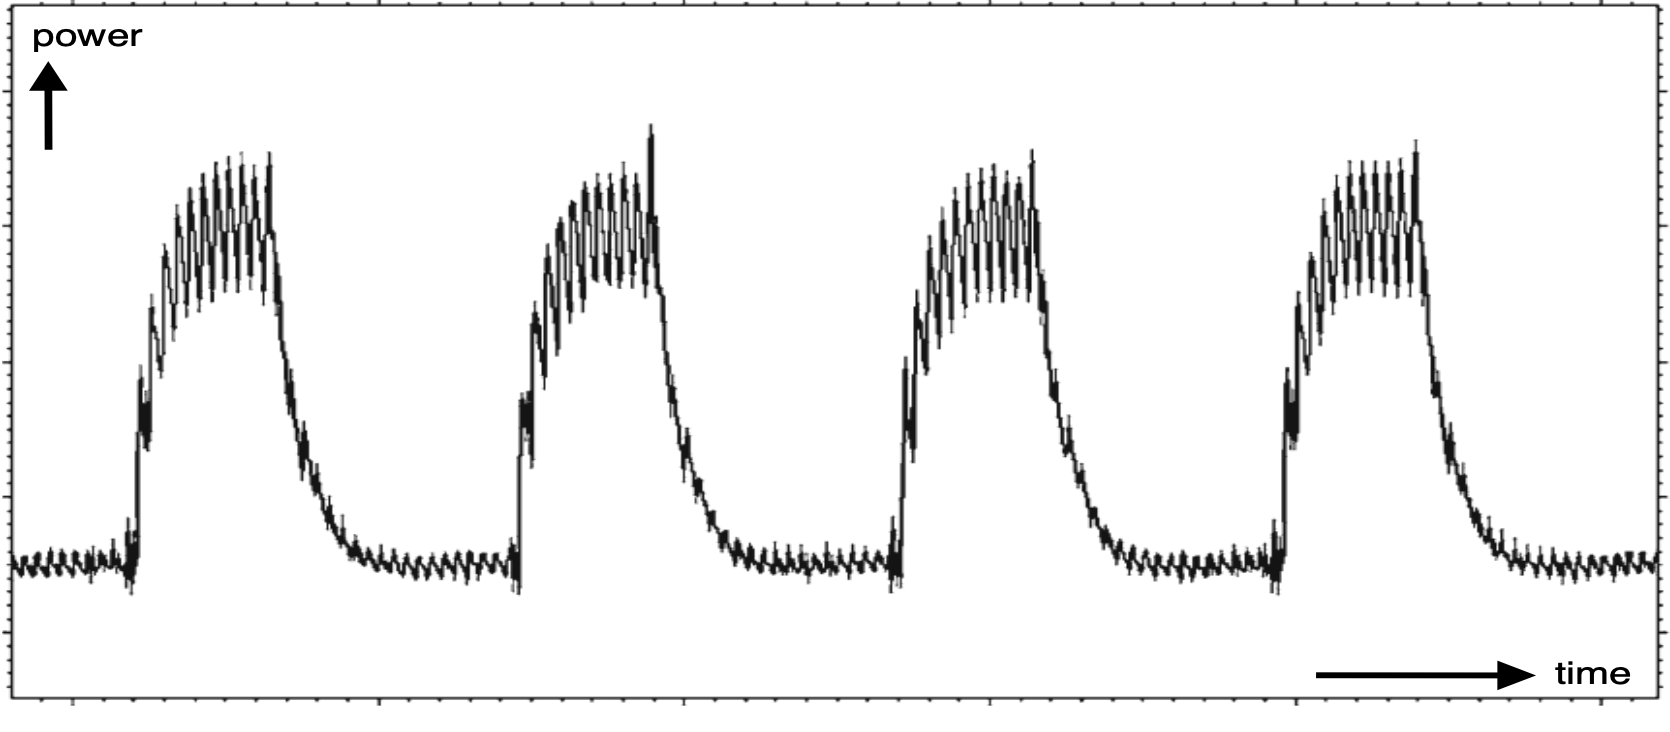
\includegraphics[width=0.4\linewidth]{figures/chapter4/fig12-a.png}
  	\label{fig:4-12-a}
  }
  \quad\quad\quad
  \subfigure[S盒LSB的输出为$0$和为$1$的情况]{
  	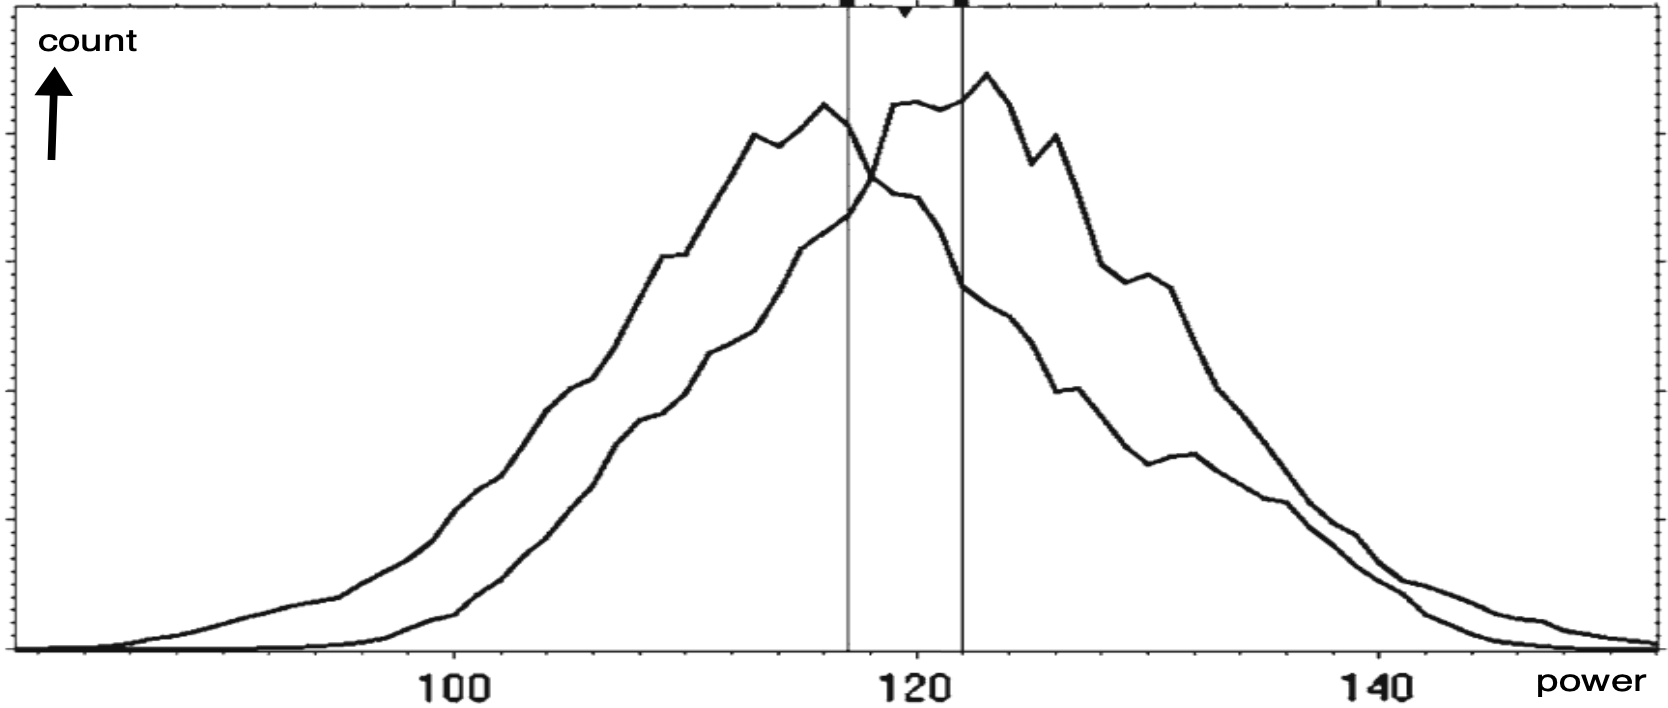
\includegraphics[width=0.4\linewidth]{figures/chapter4/fig12-b.png}
  	\label{fig:4-12-b}
  }
  
  \subfigure[功耗差分]{
  	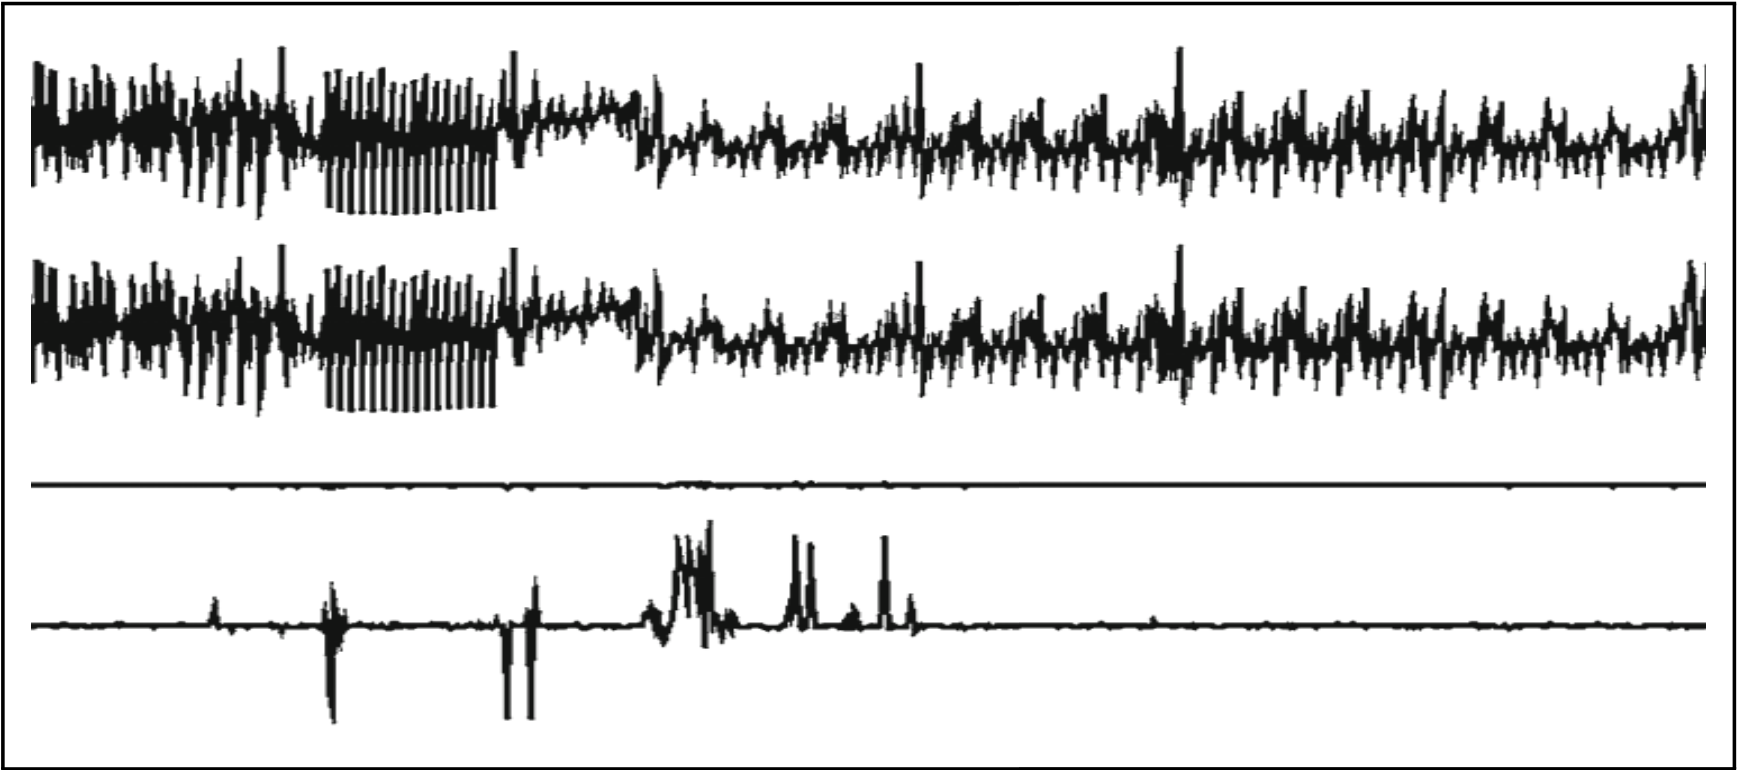
\includegraphics[width=0.4\linewidth]{figures/chapter4/fig12-c.png}
  	\label{fig:4-12-c}
  }
  \quad\quad\quad
  \subfigure[密钥$k=101,\dots,105$时的差分]{
  	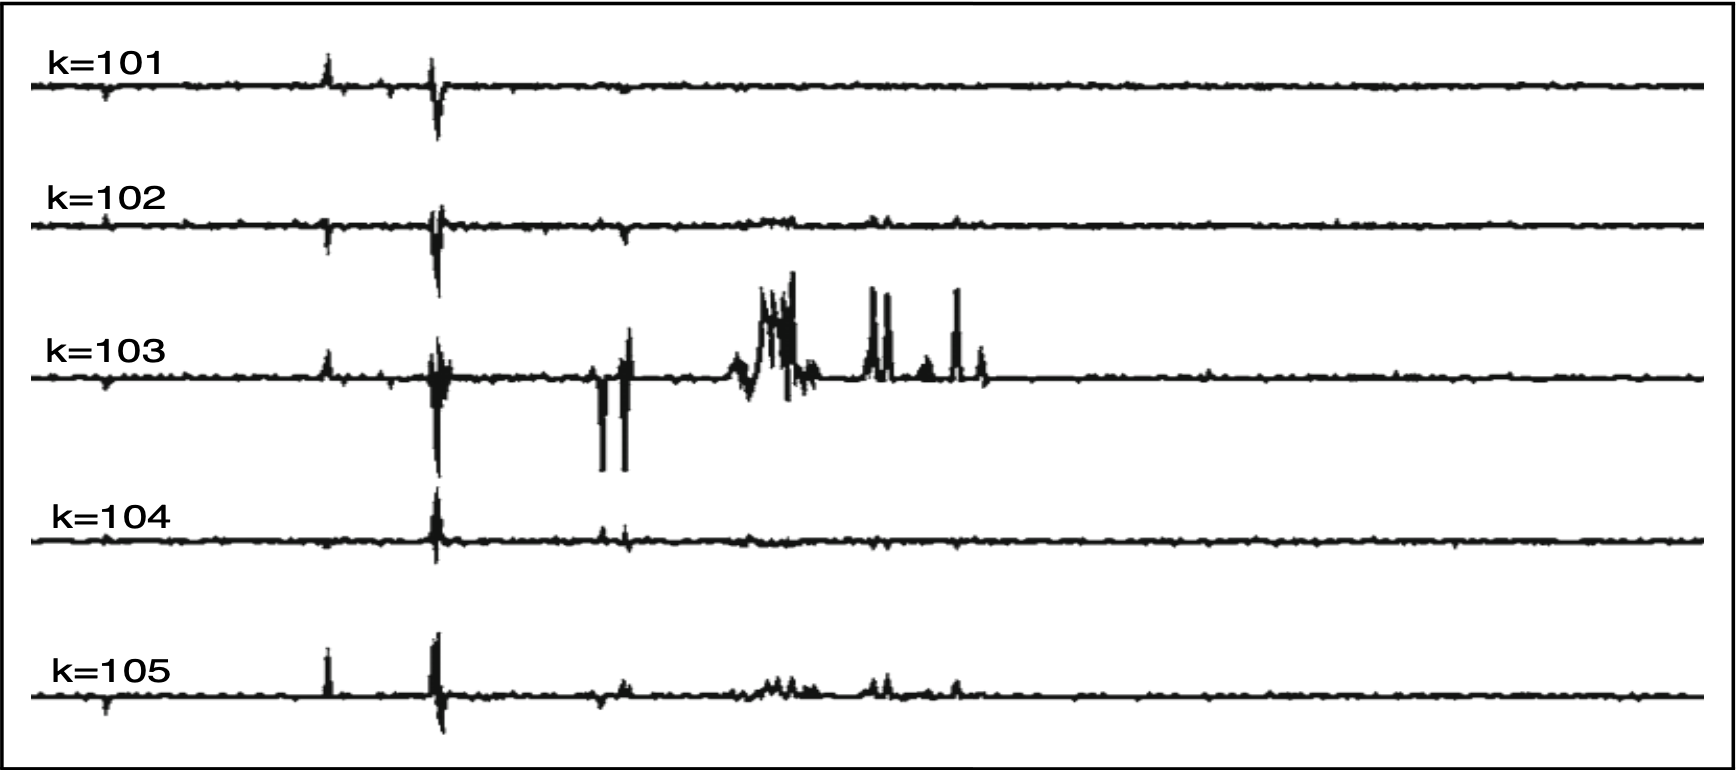
\includegraphics[width=0.4\linewidth]{figures/chapter4/fig12-d.png}
  	\label{fig:4-12-d}
  }
  \caption{针对AES的功耗分析}
\end{figure}

\begin{snote}[差分功耗分析。]
尽管 AES 对简单功耗攻击有抵抗能力,但一种更复杂的功耗攻击就能从一些简陋的 AES 算法实现中提取出 AES 密钥。随机选择一个 AES 密钥 $k$,并用它加密 $4000$ 条随机的明文。对于我们的测试设备来说,所产生的 $4000$ 个功耗轨迹图看起来非常不同,这表明在输入是随机明文的情况下,功耗轨迹与输入是相关的。

接下来,考虑第一轮中第一个 S 盒的输出,我们把这个输出称为 $T$。我们假设,S 盒查询的功耗取决于被查询的位置。也就是说,我们猜测 $T$ 的值与查表操作的功耗相关。

为了验证这个假设,我们根据 $T$ 的最小有效比特将 $4000$ 次的功率轨迹图分成两堆,第 $1$ 堆中 $T$ 的最小有效比特都为 $1$,第 $0$ 堆中 $T$ 的最小有效比特都为 $0$。考察加密信用卡在计算第一个 S 盒的输出时,每堆的功耗情况:
\begin{itemize}
	\item 第 $1$ 堆 (LSB $=1$):平均功耗 $116.9$ 个单位,标准差为 $10.7$
	\item 第 $0$ 堆 (LSB $=0$):平均功耗 $121.9$ 个单位,标准差为 $9.7$
\end{itemize}
图 \ref{fig:4-12-b} 展示了这两种功耗分布。这两个分布很接近,但有明显的不同。因此,只要有足够多的独立样本,我们就可以将两种分布区别开来。

为了利用这一观察,我们考察图 \ref{fig:4-12-c}。图中的第一行显示的是第 $1$ 堆中所有功耗轨迹的平均功耗情况。第二行显示的是第 $0$ 堆中所有功耗轨迹的平均功耗情况。最下面一行表示两条平均功耗轨迹的差分。我们可以发现,差分轨迹的第一个尖峰恰好位于计算第一个 S 盒输出时,而该尖峰的大小与图 \ref{fig:4-12-b} 中所显示的平均数之差完全对应。我们将这条差分轨迹称为\textbf{功耗差分 (power differential)}。

为了攻击目标设备,攻击者必须首先用一个干净的设备进行实验:攻击者将选定的密钥加载到设备中,并计算出设备的功耗差分轨迹,如图 \ref{fig:4-12-b} 所示。接下来,假设攻击者获得了一个带有未知的嵌入式密钥的设备,它就可以用以下方法提取密钥:
 
\vspace*{5pt}

\hspace*{5pt} 首先,对 $4000$ 条随机明文测量加密操作的功耗轨迹\\
\hspace*{26pt} 然后,对密钥首字节的每个候选值 $k\in\{0,1\}^8$,进行如下操作:\\
\hspace*{50pt} 根据 $T$ 的首个比特将 $4000$ 个样本分成两堆\\
\hspace*{75pt} (这是用目前对 $k$ 的猜测和 $4000$ 个已知的明文完成的)\\
\hspace*{50pt} 如果得到的功率差分轨迹与预先计算的曲线相匹配:\\
\hspace*{75pt} 输出 $k$ 作为密钥的首字节并停机

\vspace*{5pt}

\noindent
图 \ref{fig:4-12-d} 展示了这种攻击的效果。当使用密钥首字节的正确值(即 $k=103$)时,我们就能得到正确的功耗差分轨迹。而当使用错误的猜测($k=101,102,104,105$ 等)时,功耗差分与预期的轨迹不相符。

对 AES-128 密钥的所有 $16$ 个字节反复进行这一操作,就可以恢复整个密钥。
\end{snote}

\begin{snote}[缓和措施。]
针对功耗分析的一个常见的防御措施是进行硬件微调。从概念上讲,在执行 AES 之前,硬件会抽取固定数量的电力给电容器充电,然后利用电容器中的电力运行整个 AES 算法。一旦 AES 完成,留在电容器中的多余电量就会被丢弃。下一次应用 AES 时会再次给电容器充电,如此反复。这种概念设计(在实践中正确地实施需要一定程度的工作)旨在确保设备的功耗与设备中嵌入的密钥完全无关。

另一种缓和措施承认,每次运行解密算法都会泄露关于密钥的一些有限信息。这种措施提出在每次调用算法后重新随机化密钥,这样攻击者就不能将他从每次执行中获取到的信息结合起来。这种方法在一个被称为\textbf{抗泄露密码学 (leakage-resilient cryptography)}的领域中得到了广泛的研究。
\end{snote}

\subsection{针对AES的错误注入攻击}\label{subsec:4-3-3}

另一类攻击称为\textbf{错误注入攻击 (fault injection attack)},它试图故意在硬件运行密码系统时引入错误。攻击者可以利用畸形的输出来了解有关密钥的信息。注入错误可以通过对目标硬件进行超频,用激光加热,或对目标芯片进行电磁干扰来实现。

错误注入攻击已经被用来破解脆弱的 AES 实现,方法是迫使AES引擎在加密一个明文分组时发生故障。由此产生的畸变密文可以揭示有关密钥的信息。错误注入攻击也常被用在公钥密码场景中,我们将在 \ref{sec:17-6} 节回来详细地讨论它们,在那里,我们将介绍使用错误注入攻击完全破解 RSA 的一些实现的方法。

对错误注入攻击的一种防御措施是检查计算的结果。例如,AES 算法可以检查计算出的密文在解密后能否还原到给定的明文。如果检查失败,硬件就会抛出一个错误,并丢弃计算出的密文。但这种措施会将 AES 的性能降至原先的一半,因此不适合在实践中使用。

\subsection{量子穷举搜索攻击}\label{subsec:4-3-4}

到目前为止,我们描述的攻击都工作在经典计算机上。然而我们的物理世界是由量子力学定律所支配的。从理论上讲,人类可以构建基于量子力学定律的计算机,而这种计算机的计算能力要远超现在的经典计算机。尽管目前还没有人成功建造量子计算机,但第一台量子计算机的建成可能只是一个时间问题。

量子计算机对密码学有重大影响,因为它们可以被用来加速某些攻击,甚至完全打破一些系统。回顾一下,在经典的穷举搜索中,攻击者会得到一些用某个密钥 $k\in\mathcal{K}$ 创建的明文/密文对。攻击者会尝试所有的密钥,直到他找到一个能将给定的明文映射到给定的密文的密钥。在一台经典计算机上,这需要的时间与 $|\mathcal{K}|$ 成正比。


\begin{snote}[量子穷举搜索。]
令人惊讶的是,在量子计算机上,同样的穷举搜索的耗时只与 $\sqrt{|\mathcal{K}|}$ 成正比。这意味着对于像 AES-128 这样的分组密码,穷举搜索只需要大约 $\sqrt{2^{128}}=2^{64}$ 次计算。而使用经典计算机已经可以在合理的时间内完成 $2^{64}$ 步的计算,所以一旦量子计算机建成,它们也将能够进行这种规模的计算。因此,一旦量子计算机被制造出来,AES-128 将被认为是不安全的。

上述讨论表明,一个分组密码想要抵御量子穷举搜索攻击,其密钥空间 $|\mathcal{K}|$ 必须至少有 $2^{256}$ 那么大。此时,量子穷举搜索的时间是 $2^{128}$ 数量级的。量子计算机的这种威胁是 AES 支持 $256$ 比特密钥的原因之一。当然,我们不能保证没有更快的量子算法来破解 AES-256,但至少量子穷举搜索是不可能的。
\end{snote}

\begin{snote}[格罗弗算法。]
量子穷举搜索算法是量子计算中一个更一般结论的特例,该结论由洛夫·格罗弗 (Lov Grover) 提出。该结论表明:假设我们有一个函数 $f:\mathcal{K}\to\{0,1\}$,对于某个 $k_0\in\mathcal{K}$,$f$ 的定义如下:
\begin{equation}\label{eq:4-20}
f(k)=\left\{
\begin{array}{ll}
1, & k=k_0\\
0, & k\neq k_0
\end{array}
\right.
\end{equation}
我们的目标是在只能黑箱访问 $f$(即只能在不同的输入情况下查询$f$的输出)的情况下找到 $k_0$。在经典计算机上,没有任何其他方法的效率高于穷举所有的 $k\in\mathcal{K}$,在最糟糕的情况下,这需要对 $f$ 进行 $|\mathcal{K}|$ 数量级的查询。

格罗弗算法表明,在量子计算机上只需 $O\big(\sqrt{|K|}\cdot{\rm time}(f)\big)$ 步就可以找到 $k_0$,其中 ${\rm time}(f)$ 表示计算 $f(x)$ 的耗时。这是个结论是普适的,它对任何形如式 \ref{eq:4-20} 的函数 $f$ 都成立。该结论可以用于加速一般的硬优化问题,是量子计算机的杀手锏。

在给定若干明文/密文对的情况下,为了破解一个像 AES-128 这样的分组密码,我们定义函数:
\[
f_{\rm AES}(k)=\left\{
\begin{array}{ll}
1, & {\rm AES}(k,\overline m)=\bar c\\
0, & {\rm AES}(k,\overline m)\neq\bar c
\end{array}
\right.
\]
其中 $\overline m=(m_0,\dots,m_Q)$,$\bar c=(c_0,\dots,c_Q)$ 是给定的明文和密文分组。假设给定足够多的分组,则必有唯一密钥 $k_0\in\mathcal{K}$ 满足 ${\rm AES}(k_0,\overline m)=\bar c$。而格罗弗算法可以在 $\sqrt{|\mathcal{K}|}$ 数量级的时间内找到这个密钥。
\end{snote}
\section{伪随机函数:基本定义与性质}

虽然安全的分组密码是许多密码系统的组成部分,但一个与之密切相关的概念,即伪随机函数(PRF),被证明是许多应用中的正确工具。PRF在概念上比分组密码更加简单,正如我们将看到的,它们有着广泛的应用。PRF和分组密码密切相关,在某些假设下,我们可以用安全的分组密码作为安全伪随机函数的替身。这种性质非常有益,因为正如我们在上一节所看到的,我们已经有了许多非常实用的、貌似安全的分组密码。

\subsection{定义}

\textbf{伪随机函数 (Pseudo-random function, PRF)} $F$ 是一种确定性算法,它有两个输入:一个密钥 $k\in\mathcal{K}$ 和一个\textbf{输入数据分组} $x\in\mathcal{X}$;它的输出 $y:=F(k,x)\in\mathcal{Y}$ 被称为\textbf{输出数据分组}。我们称 $F$ \textbf{定义在} $(\mathcal{K},\mathcal{X},\mathcal{Y})$ \textbf{上}。

直观地讲,我们对伪随机函数的安全概念表明,对于一个随机选择的密钥 $k$,函数 $F(k,\cdot)$ 对于所有实际目的都应该是一个``看起来像"随机分布的一个从 $\mathcal{X}$ 到 $\mathcal{Y}$ 的映射。为了使这一概念更加精确,我们首先引入一些符号:
\[
{\rm Funs}[\mathcal{X},\mathcal{Y}]
\]
表示\emph{所有}函数 $f:\mathcal{X}\to\mathcal{Y}$ 构成的集合。这是一个非常大的集合,事实上:
\[
|{\rm Funs}[\mathcal{X},\mathcal{Y}]|=|\mathcal{Y}|^{|\mathcal{X}|}
\]

我们可以定义如下的攻击游戏:

\begin{game}[伪随机函数]\label{game:4-2}
对于一个给定的定义在 $(\mathcal{K},\mathcal{X},\mathcal{Y})$ 上的 PRF $F$,对于一个给定对手 $\mathcal{A}$,我们定义两个实验:实验$0$和实验$1$。对于$b=0,1$,我们定义:\\
\noindent\textbf{实验$b$:}
\begin{itemize}
	\item 挑战者按照如下方式选定 $f\in{\rm Funs}[\mathcal{X},\mathcal{Y}]$:
	\vspace{1pt}
	
	\hspace*{5pt} 如果 $b=0$:选取 $k\overset{\rm R}\leftarrow\mathcal{K}$,令 $f\leftarrow F(k,\cdot)$;\\
	\hspace*{5pt} 如果 $b=1$:选取 $f\overset{\rm R}\leftarrow{\rm Funs}[\mathcal{X},\mathcal{Y}]$。
	\item 对手向挑战者提交一连串的查询。\\
	对于 $i=1,2,\dots$,第 $i$ 次查询是一个输入数据分组 $x_i\in\mathcal{X}$。\\
	挑战者计算 $y_i\leftarrow f(x_i)\in\mathcal{Y}$,并将 $y_i$ 交给对手。
	\item 对手计算并输出一个比特 $\hat{b}\in\{0,1\}$。
\end{itemize}
对于 $b=0,1$,令 $W_b$ 为 $\mathcal{A}$ 在实验 $b$ 中输出 $1$ 的事件。我们将 $\mathcal{A}$ 相对于 $F$ 的\textbf{优势}定义为:
\begin{equation}\label{eq:4-21}
{\rm PRF\mathsf{adv}}[\mathcal{A}, F]:=
\Big\lvert
{\rm Pr}[W_0]-{\rm Pr}[W_1]
\Big\rvert
\end{equation}
如果对手 $\mathcal{A}$ 最多发出 $Q$ 次查询,我们就称 $\mathcal{A}$ 是一个 \textbf{$Q$ 次查询伪随机函数对手($Q$-query PRF adversary)}。
\end{game}

\begin{definition}[安全的 PRF]\label{def:4-2}
如果对于所有的有效对手 $\mathcal{A}$,${\rm PRF\mathsf{adv}}[\mathcal{A},F]$ 的值都可忽略不计,我们就称伪随机函数 $F$ 是\textbf{安全的}。
\end{definition}

需要再次强调,在攻击游戏 \ref{game:4-2} 中,对手所做的查询可以是自适应的:对手可以根据挑战者之前应答的内容来构造每个新的查询(见练习 \ref{exer:4-6})。

正如 \ref{subsec:2-2-5} 小节所讨论的,攻击游戏 \ref{game:4-2} 可以被重构为一个``比特猜测"游戏。在该游戏中,挑战者并不运行两个独立的实验,而是随机选择一个 $b\in\{0,1\}$,然后针对对手 $\mathcal{A}$ 运行实验 $b$。在这个游戏中,我们令 $\mathcal{A}$ 的比特猜测优势 ${\rm PRF\mathsf{adv}}^*[\mathcal{A}, F]$ 为 $|{\rm Pr}[\hat{b}=b]-{1}/{2}|$。那么,\ref{subsec:2-2-5} 小节中的推广结论(即式 \ref{eq:2-11})在此也适用:
\begin{equation}
{\rm PRF\mathsf{adv}}[\mathcal{A}, F]=2\cdot {\rm PRF\mathsf{adv}}^*[\mathcal{A}, F]
\end{equation}

\begin{snote}[弱安全的伪随机函数。]
对于某些使用 PRF 的构造来说,PRF 满足比定义 \ref{def:4-2} 更弱的安全属性也就足够了。我们说,如果对手的查询受到严格限制,但仍没有有效对手能够将 PRF 与随机函数区分开来时,我们就说该 PRF 是\emph{弱安全的}。所谓的查询的严格限制,指的是对手只能在域中的\emph{随机}点上查询函数。将对手的查询限制在随机输入上,就有可能更容易建立弱安全的 PRF。在练习 \ref{exer:4-2} 中,我们会研究弱安全但不完全安全的自然 PRF 构造。

我们通过稍微修改攻击游戏 \ref{game:4-2} 来定义弱安全的 PRF。假设 $F$ 是一个定义在 $(\mathcal{K},\mathcal{X},\mathcal{Y})$ 上的 PRF。现在,我们修改对手 $\mathcal{A}$ 与挑战者的交互方式:每当对手 $\mathcal{A}$ 查询函数时,挑战者都选择一个随机数 $x\in\mathcal{X}$,并将 $x$ 与 $f(x)$ 都发送给对手。换句话说,对手 $\mathcal{A}$ 看到的是函数 $f$ 在 $\mathcal{X}$ 上的一个\emph{随机}点上的评估结果,并且需要判断该函数是真正的随机函数还是一个伪随机函数。我们将对手 $\mathcal{A}$ 在该游戏中的优势定义为 ${\rm wPRF\mathsf{adv}}[\mathcal{A}, F]$,如式 \ref{eq:4-21} 所示。
\end{snote}

\begin{definition}[弱安全的 PRF]\label{def:4-3}
如果对于所有的有效对手 $\mathcal{A}$, ${\rm wPRF\mathsf{adv}}[\mathcal{A}, F]$ 的值都可忽略不计,我们就称伪随机函数 $F$ 是\textbf{弱安全的}。
\end{definition}

\subsection{随机函数的有效实现}\label{subsec:4-4-2}

同 \ref{subsec:4-1-2} 小节一样,我们可以通过一个\textbf{忠实的侏儒}来实现攻击游戏 \ref{game:4-2} 的实验 $1$ 中挑战者使用的从 ${\rm Funs}[\mathcal{X},\mathcal{Y}]$ 中选出的随机函数。同分组密码的情况一样,挑战者会跟踪输入/输出对 $(x_i,y_i)$。当挑战者收到第 $i$ 次查询 $x_i$ 时,它需要验证是否存在某个 $j < i$ 使得 $x_i=x_j$ 成立。如果存在,它就令 $y_i\leftarrow y_j$(这确保挑战者确实实现了一个函数),否则就从集合 $\mathcal{Y}$ 中随机选择一个 $y_i$;最后,挑战者将 $y_i$ 发送给对手。我们可以把挑战者的这种实现逻辑表述如下:

\vspace{5pt}

\hspace*{5pt} 当从对手 $\mathcal{A}$ 处收到第 $i$ 个查询 $x_i\in\mathcal{X}$ 时:\\
\hspace*{50pt} 如果存在某个 $j<i$ 使得 $x_i=x_j$ 成立:\\
\hspace*{75pt} 令 $y_i\leftarrow y_j$\\
\hspace*{75pt} 否则,选取 $y_i\overset{\rm R}\leftarrow\mathcal{Y}$\\
\hspace*{50pt} 将 $y_i$ 发送给 $\mathcal{A}$。\\

\subsection{什么时候一个安全的分组密码是安全的PRF?}

在本小节的开始,我们提出一个问题:什么时候一个安全分组密码才是一个安全的 PRF?在回答这个问题时,我们要介绍一种在整个密码学中被大量使用的证明技术。

令 $\mathcal{E}=(E,D)$ 是一个定义在 $(\mathcal{K},\mathcal{X})$ 上的分组密码,并令 $N:=|\mathcal{X}|$。我们可以自然地把 $\mathcal{E}$ 看作是一个定义在 $(\mathcal{K},\mathcal{X},\mathcal{X})$ 上的 PRF。现在假设 $\mathcal{E}$ 是一个安全分组密码,也就是说,不存在有效对手能够有效地将 $\mathcal{E}$ 与随机置换区分开来。这是否意味着 $\mathcal{E}$ 也是一个安全的 PRF 呢?也即,这是否意味着不存在有效对手可以有效地将 $\mathcal{E}$ 与随机函数区分开来?

这个问题的答案是``是",前提是 $N$ 是超多项式的。在论证这个问题之前,我们需要先论证,当 $N$ 很小的时候,上述问题的答案``否"。

考虑一个 PRF 对手,它对 $\mathcal{E}$ 进行攻击游戏 \ref{game:4-2} 中所描述的攻击,令 $f$ 是挑战者选择的函数:在实验 $0$ 中,$f=E(k,\cdot)$,其中 $k\in\mathcal{K}$ 为一随机值;而在实验 $1$ 中,$f$ 是从 ${\rm Funs}[\mathcal{X},\mathcal{Y}]$ 中随机选出的。假设 $N$ 是如此之小,以至于一个有效对手可以对所有的 $x\in\mathcal{X}$ 计算 $f(x)$ 的值。此外,如果对手 $\mathcal{A}$ 看到了两个不同的 $x,x'\in\mathcal{X}$ 使得 $f(x)=f(x')$,它就输出 $1$,否则就输出 $0$。显然,在实验 $0$ 中,$\mathcal{A}$ 输出 $1$ 的概率为 $0$,因为此时 $f=E(k,\cdot)$ 是一个置换。然而,在实验 $1$ 中,$\mathcal{A}$ 能以 $1-{N!}/{N^N}\geq{1}/{2}$ 的概率输出 $1$。因此我们有 ${\rm PRF\mathsf{adv}}[\mathcal{A}, F]\geq{1/2}$,所以 $\mathcal{E}$ 不是一个安全的 PRF。

上述论证可以用生日悖论来完善(见附录 \ref{sec:B-1} 节)。对于任何多项式边界的 $Q$,我们可以定义一个有效 PRF 对手 $\mathcal{A}$,它对 $\mathcal{E}$ 进行攻击游戏 \ref{game:4-2} 中的攻击,流程如下所述。对手 $\mathcal{A}$ 只需向挑战者发出 $Q$ 个不同的查询,当且仅当它能得到两个不同的值 $x,x'\in\mathcal{X}$ (从给挑战者的$Q$个值中选出)使得 $f(x)=f(x')$时,输出 $1$。同样,在实验 $0$ 中,$\mathcal{A}$ 输出 $1$ 的概率为 $0$。然而,根据定理 \ref{theo:B-1},在实验 $1$ 中,$\mathcal{A}$ 输出 $1$ 的概率至少为 $\min\{{Q(Q-1)}/{4N},0.63\}$。因此,只需进行 $O(N^{1/2})$ 次查询,对手就可以很容易地看到,置换的行为并不像是一个随机函数。

事实证明,``生日攻击"是所有对手所能达到的最好情况。当 $N$ 是超多项式的时候,这种攻击就变得不再可行了。

\begin{theorem}[PRF 切换引理]\label{theo:4-4}
令 $\mathcal{E}=(E,D)$ 是一个定义在 $(\mathcal{K},\mathcal{X})$ 上的分组密码,并令 $N:=|\mathcal{X}|$。令 $\mathcal{A}$ 是一个对手,它最多向挑战者发起 $Q$ 次查询。则有:
\[
\Big\lvert
{\rm BC\mathsf{adv}}[\mathcal{A},\mathcal{E}]-{\rm PRF\mathsf{adv}}[\mathcal{A},\mathcal{E}]
\Big\rvert
\leq{Q^2}/{2N}
\]
\end{theorem}

在证明这个定理之前,我们先导出下面的一个简单的推论。

\begin{corollary}\label{cor:4-5}
令 $\mathcal{E}=(E,D)$ 是一个定义在 $(\mathcal{K},\mathcal{X})$ 上的分组密码,并假设 $N:=|\mathcal{X}|$ 是超多项式的。那么,当且仅当 $\mathcal{E}$ 是一个安全的 PRF 时,$\mathcal{E}$ 是一个安全的分组密码。
\end{corollary}

\begin{proof}
根据定义,如果 $\mathcal{A}$ 是一个有效对手,它向挑战者发出的最大查询次数 $Q$ 是多项式边界的。因此,根据定理 \ref{theo:4-4},我们有:
\[
\Big\lvert
{\rm BC\mathsf{adv}}[\mathcal{A},\mathcal{E}]-{\rm PRF\mathsf{adv}}[\mathcal{A},\mathcal{E}]
\Big\rvert
\leq{Q^2}/{2N}
\]
由于 $N$ 是超多项式的,$Q$ 是多项式边界的,所以 $\frac{Q^2}{2N}$ 是可以忽略不计的(见事实 \ref{fact:2-6})。由此可见,当且仅当 ${\rm PRF\mathsf{adv}}[\mathcal{A},\mathcal{E}]$ 可忽略不计时,${\rm BC\mathsf{adv}}[\mathcal{A},\mathcal{E}]$ 才是可以忽略不计的。
\end{proof}

实际上,定理 \ref{theo:4-4} 的证明与分组密码和 PRF 无关,它实际上是一个关于随机置换和随机函数的论证。让我们定义一个新的攻击游戏,用以测试对手区分随机置换与随机函数的能力。

\begin{game}[置换 \emph{vs.} 函数]\label{game:4-3}
对于一个给定有限集 $\mathcal{X}$ 和一个给定对手 $\mathcal{A}$,我们定义两个实验:实验$0$和实验$1$。对于$b=0,1$,我们定义:\\
\textbf{实验$b$:}
\begin{itemize}
	\item 挑战者按照如下方式选定 $f\in{\rm Funs}[\mathcal{X},\mathcal{X}]$:
	\vspace{1pt}
	
	\hspace*{5pt} 如果 $b=0$:选取 $f\overset{\rm R}\leftarrow{\rm Perms}[\mathcal{X}]$;\\
	\hspace*{5pt} 如果 $b=1$:选取 $f\overset{\rm R}\leftarrow{\rm Funs}[\mathcal{X},\mathcal{X}]$。
	\item 对手向挑战者提交一连串的查询。\\
	对于 $i=1,2,\dots$,第 $i$ 次查询是一个输入数据分组 $x_i\in\mathcal{X}$。\\
	挑战者计算 $y_i\leftarrow f(x_i)\in\mathcal{Y}$,并将 $y_i$ 交给对手。
	\item 对手计算并输出一个比特 $\hat{b}\in\{0,1\}$。
\end{itemize}
对于 $b=0,1$,令 $W_b$ 为 $\mathcal{A}$ 在实验 $b$ 中输出 $1$ 的事件。我们将 $\mathcal{A}$ 相对于 $\mathcal{X}$ 的\textbf{优势}定义为:
\[
{\rm PF\mathsf{adv}}[\mathcal{A}, \mathcal{X}]:=
\Big\lvert
{\rm Pr}[W_0]-{\rm Pr}[W_1]
\Big\rvert
\]
\end{game}

\begin{theorem}\label{theo:4-6}
令 $\mathcal{X}$ 是一个大小为 $N$ 的有限集,$\mathcal{A}$ 是一个对手,它最多向挑战者发起 $Q$ 次查询,则有:
\[
{\rm PF\mathsf{adv}}[\mathcal{A},\mathcal{X}]\leq{Q^2}/{2N}
\]
\end{theorem}


我们首先表明,上面的定理很容易推出定理 \ref{theo:4-4}。

\begin{proof}[定理 \ref{theo:4-4} 的证明]
令 $\mathcal{E}=(E,D)$ 是一个定义在 $(\mathcal{K},\mathcal{X})$ 上的分组密码。令 $\mathcal{A}$ 是一个对手,它最多向挑战者发起 $Q$ 次查询。我们定义游戏 $0$、游戏 $1$ 和游戏 $2$,它们都在 $\mathcal{A}$ 和挑战者之间进行。对于 $j=0,1,2$,我们定义 $p_j$ 为 $\mathcal{A}$ 在游戏 $j$ 中输出 $1$ 的概率。在每个游戏中,挑战者根据特定的分布选择一个函数 $f:\mathcal{X}\to\mathcal{X}$,并以 $f(x)$ 来应答 $\mathcal{A}$ 的每个查询 $x\in\mathcal{X}$。

\noindent\textbf{游戏 $\mathbf{0}$}:该游戏中的挑战者令 $f:=E(k,\cdot)$,其中 $k\in\mathcal{K}$ 是随机选出的。

\noindent\textbf{游戏 $\mathbf{1}$}:该游戏中的挑战者随机选择 $f\in{\rm Perms}[\mathcal{X}]$。

\noindent\textbf{游戏 $\mathbf{2}$}:该游戏中的挑战者随机选择 $f\in{\rm Funs}[\mathcal{X},\mathcal{X}]$。

注意到,根据定义,有:
\[
\begin{aligned}
	& |p_1-p_0| = {\rm BC\mathsf{adv}}[\mathcal{A},\mathcal{E}]\\
	& |p_2-p_0| = {\rm PRF\mathsf{adv}}[\mathcal{A},\mathcal{E}]
\end{aligned}
\]
而根据定理 \ref{theo:4-6},有:
\[
|p_2-p_1|={\rm PF\mathsf{adv}}[\mathcal{A},\mathcal{X}]\leq{Q^2}/{2N}
\]
将上两式结合,我们得到:
\[
\big\lvert
{\rm BC\mathsf{adv}}[\mathcal{A},\mathcal{E}]-{\rm PRF\mathsf{adv}}[\mathcal{A},\mathcal{E}]
\big\rvert
=
\big\lvert
|p_1-p_0|-|p_2-p_0|
\big\rvert
\leq|p_2-p_1|\leq{Q^2}/{2N}
\]

这就证明了该定理。
\end{proof}

所以,剩下工作的就是证明定理 \ref{theo:4-6}。在此之前,我们要说明一个非常简单但非常有用的结论:

\begin{theorem}[差分引理]\label{theo:4-7}
令 $Z$,$W_0$,$W_1$ 是定义在某个概率空间上的事件。假设当且仅当 $W_1\land\bar Z$ 发生时,$W_0\land\bar Z$ 才发生,则我们有:
\[
|\Pr[W_0]-\Pr[W_1]|\leq\Pr[Z]
\]
\end{theorem}

\begin{proof}
这就是一个简单的计算。我们有:
\[
\begin{aligned}
|\Pr[W_0]-\Pr[W_1]|
&=|\Pr[W_0\land Z]+\Pr[W_0\land\bar Z]-\Pr[W_1\land Z]-\Pr[W_1\land\bar Z]|\\
&=|\Pr[W_0\land Z]-\Pr[W_1\land Z]|\\
&\leq \Pr[Z]
\end{aligned}
\]
其中第二个等式来自 $W_0\land\bar{Z} \Longleftrightarrow W_1\land\bar{Z}$ 的假设,所以,一个特殊结论就是 $\Pr[W_0\land\bar{Z}]=\Pr[W_1\land\bar{Z}]$。最后的不等式来自于这样一个事实,即 $\Pr[W_0\land Z]$ 和 $\Pr[W_1\land Z]$ 都是介于 $0$ 和 $\Pr[Z]$ 之间的值。
\end{proof}
 
在我们对差分定理的大多数应用中,$W_0$ 代表一个给定对手在对某个挑战者的游戏中输出 $1$ 的事件,而 $W_1$ 则是同一个对手在对另一个挑战者的游戏中输出 $1$ 的事件。为了应用差分定理,我们定义这两个游戏,使它们都在相同的基础概率空间上运行。这意味着我们假设对手和挑战者在两个游戏中所做的随机选择都是一样的,两个游戏的不同之处仅在于挑战者针对来自对手的查询给出反馈的策略。

\begin{proof}[定理 \ref{theo:4-6} 的证明]
考虑一个对手 $\mathcal{A}$,它对 $\mathcal{X}$ 进行攻击游戏 \ref{game:4-3} 中的攻击,其中 $N:=|\mathcal{X}|$,并假设 $\mathcal{A}$ 最多向挑战者发起 $Q$ 次查询。考虑这个攻击游戏的实验 $0$。利用 \ref{subsec:4-4-2} 小节讨论的``忠实的侏儒"的思想,我们可以通过跟踪输入/输出对 $(x_i,y_i)$ 来实现实验 $0$;此外,为 $y_i$ 选择初始的``默认"值 $z_i$ 是很方便的,$z_1,\dots,z_Q$ 可以从 $\mathcal{X}$ 中均匀独立随机选出;这些``默认"值在必要时可以被覆写,以确保挑战者定义的是一个随机置换。下面是详细的过程:

\vspace{5pt}

\hspace*{5pt} 选取 $z_1,\dots,z_Q\overset{\rm R}\leftarrow\mathcal{X}$\\
\hspace*{26pt} 当收到 $\mathcal{A}$ 的第 $i$ 个查询 $x_i$ 时:\\
\hspace*{50pt} 如果存在某个 $j<i$ 使得 $x_i=x_j$,则:\\
\hspace*{75pt} 令 $y_i\leftarrow y_j$\\
\hspace*{50pt} 否则:\\
\hspace*{75pt} 令 $y_i\leftarrow z_i$\\
\hspace*{1pt} ($*$)
\hspace*{53pt} 如果 $y_i\in\{y_1,\dots,y_{i-1}\}$,则选取 $y_i\overset{\rm R}\leftarrow\mathcal{X}\setminus\{y_1,\dots,y_{i-1}\}$;\\
\hspace*{50pt} 将 $y_i$ 发送给 $\mathcal{A}$。

\vspace{5pt}

标有 ($*$) 的那行用于测试是否需要覆盖默认值 $z_i$,确保没有任何输出值被用于两个不同的输入值。

令 $W_0$ 为 $\mathcal{A}$ 在该游戏中输出 $1$ 的事件,我们称之为游戏 $0$。

我们现在修改上述挑战者的实现,得到另一个新的游戏:

\vspace{5pt}

\hspace*{5pt} 选取 $z_1,\dots,z_Q\overset{\rm R}\leftarrow\mathcal{X}$\\
\hspace*{26pt} 当收到 $\mathcal{A}$ 的第 $i$ 个查询 $x_i$ 时:\\
\hspace*{50pt} 如果存在某个 $j<i$ 使得 $x_i=x_j$,则:\\
\hspace*{75pt} 令 $y_i\leftarrow y_j$\\
\hspace*{50pt} 否则:\\
\hspace*{75pt} 令 $y_i\leftarrow z_i$\\
\hspace*{50pt} 将 $y_i$ 发送给 $\mathcal{A}$。

\vspace{5pt}

我们所做的只是在原来的挑战者逻辑中删除了标有 ($*$) 的那行,这使得我们``忠实的侏儒"变成了一个``健忘的侏儒",它忘记了检查输出值是否存在重复。

令 $W_1$ 为 $\mathcal{A}$ 在与这个修改后的挑战者进行的游戏中输出 $1$ 的事件,我们称之为游戏 $1$。

请注意,游戏 $1$ 等同于攻击游戏 \ref{game:4-3} 的实验 $1$;特别地,$\Pr[W_1]$ 等于 $\mathcal{A}$ 在攻击游戏 \ref{game:4-3} 的实验 $1$ 中输出 $1$ 的概率。因此,我们有:
\[
{\rm PF\mathsf{adv}}[\mathcal{A},\mathcal{X}]=|\Pr[W_0]-\Pr[W_1]|
\]

我们现在应用差分引理。为此,上述两个游戏都被假设运行在相同的基础概率空间上。在这两个游戏中,对手和挑战者所做的所有随机选择都是一样的,唯一不同的是挑战者用来给出应答的规则。特别地,这意味着 $\mathcal{A}$ 的随机选择和挑战者选择的值 $z_1,\dots,z_Q$ 不仅具有相同的分布,而且在两个游戏中都是\emph{确确实实的相同值}。

定义 $Z$ 为存在某个 $i\neq j$ 使得 $z_i=z_j$ 成立的事件。现在,假设我们运行游戏 $0$ 和游戏 $1$,而事件 $Z$ 没有发生。这意味着 $z_i$ 的值都是不同的。现在,由于对手的随机选择在两个游戏中都是相同的,它在两个游戏中的第一次查询也是相同的,因此挑战者的应答在两个游戏中也是相同的。对手的第二次查询(是其随机选择和挑战者第一次应答的函数)在两个游戏中也都是一样的。由于我们假设 $Z$ 没有发生,挑战者的应答在两个游戏中是相同的。继续这个论证,我们可以看到,对手的每次查询和挑战者的每个应答在两个游戏中都是一样的,因此对手的输出在两个游戏中都是一样的。因此,如果 $Z$ 没有发生,对手在游戏 $0$ 中输出 $1$,那么它在游戏 $1$ 中也会输出 $1$。同样地,如果 $Z$ 没有发生,而对手在游戏 $1$ 中输出 $1$,那么它在游戏 $0$ 中也会输出 $1$。更简洁地说,当且仅当 $W_1\land\bar{Z}$ 发生时,我们有 $W_0\land\bar{Z}$ 发生。因此,差分引理适用于该场景,我们得到:
\[
|\Pr[W_0]-\Pr[W_1]|\leq\Pr[Z]
\]

剩下的就是确定 $\Pr[Z]$ 的上界。这可由联合约束得到:对于任意不同索引对 $(i,j)$,必有$\Pr[z_i=z_j]={1}/{N}$,由于这样的索引对至多有 ${Q^2}/{2}$ 对,因此有:
\[
\Pr[Z]\leq{Q^2}/{2N}
\]
因此该定理得证。
\end{proof}

尽管还有其他的策略可以用来证明前面的定理(见练习 \ref{exer:4-24}),但我们在上面的证明中所使用的\textbf{健忘的侏儒}技术是非常有用的,我们将在后面的文章中多次看到它。

\subsection{使用 PRF 构建 PRG}\label{subsec:4-4-4}

由一个 PRF 构造一个 PRG 是很容易的。令 $F$ 是一个定义在 $(\mathcal{K},\mathcal{X},\mathcal{Y})$ 上的 PRF,$l\geq1$ 是一个多项式边界的值,令 $x_1,\dots,x_l$ 是 $\mathcal{X}$ 中任意固定且互不相同的元素(这要求$|\mathcal{X}|\geq l$)。我们定义一个具有种子空间 $\mathcal{K}$ 和输出空间 $\mathcal{Y}^l$ 的 PRG 如下:对于 $k\in\mathcal{K}$:
\[
G(k):=
\big(
F(k,x_1),\dots,F(k,x_l)
\big)
\]

\begin{theorem}\label{theo:4-8}
如果 $F$ 是一个安全的 PRF,那么上述 PRG $G$ 就是一个安全的 PRG。
\begin{quote}
特别地,对于每一个就 $G$ 进行攻击游戏 \ref{game:3-1} 的 PRG 对手 $\mathcal{A}$,都存在一个就 $F$ 进行攻击游戏 \ref{game:4-2} 的 PRF 对手 $\mathcal{B}$,其中 $\mathcal{B}$ 是一个围绕 $\mathcal{A}$ 的基本包装器,满足:
\end{quote}
\[
\mathrm{PRG}\mathsf{adv}[\mathcal{A},G]= 
\mathrm{PRF}\mathsf{adv}[\mathcal{B},F]
\]
\end{theorem}

\begin{proof}
令 $\mathcal{A}$ 是一个有效 PRG 对手,它对 $G$ 进行攻击游戏 \ref{game:3-1} 中的攻击。我们描述一个相应的 PRF 对手 $\mathcal{B}$,它对 $F$ 进行攻击游戏 \ref{game:4-2} 中的攻击。对手 $\mathcal{B}$ 的工作方式如下:
\begin{quote}
$\mathcal{B}$ 向它的挑战者发起查询 $x_1,\dots,x_\ell$ 并获得应答 $y_1,\dots,y_\ell$。然后,对手 $\mathcal{B}$ 扮演 $\mathcal{A}$ 的挑战者的角色,向 $\mathcal{A}$ 发送 $(y_1,\dots,y_\ell)$。最后,对手 $\mathcal{B}$ 原样输出 $\mathcal{A}$ 所输出的所有东西。
\end{quote}

从构造上看,对于 $b=0,1$,$\mathcal{B}$ 在攻击游戏 \ref{game:4-2} 的实验 $b$ 相对于 $F$ 输出 $1$ 的概率恰好等于 $\mathcal{A}$ 在攻击游戏 \ref{game:3-1} 的实验 $b$ 相对于 $G$ 输出 $1$ 的概率,因此定理立即得证。
\end{proof}

\subsubsection{确定性计数器模式}

上述构造为我们提供了另一种从安全分组密码中建立语义安全密码的方法。假设 $\mathcal{E}=(E,D)$ 是一个定义在 $(\mathcal{K},\mathcal{X})$ 上的分组密码,其中 $\mathcal{X}=\{0,1\}^n$。令 $N:=|\mathcal{X}|=2^n$,假设 $N$ 是超多项式的,并且 $\mathcal{E}$ 是一个安全的分组密码。那么根据定理 \ref{theo:4-4},加密函数 $\mathcal{E}$ 是一个定义在 $(\mathcal{K},\mathcal{X},\mathcal{X})$ 上的安全 PRF。然后我们可以将定理 \ref{theo:4-8} 应用于 $\mathcal{E}$  以得到一个安全 PRG,最后将定理 \ref{theo:3-1} 应用于这个 PRG,最终得到一个语义安全的流密码。

让我们详细考察这个流密码。这个密码 $\mathcal{E}'=(E',D')$ 具有密钥空间 $\mathcal{K}$ 以及消息和密文空间 $\mathcal{X}^{\leq\ell}$,其中 $\ell$ 是一个多项式边界的值,特别是 $\ell\leq N$。我们可以将 $x_1,\dots,x_\ell$ 定义为 $\mathcal{X}$ 上任何方便的元素;特别地,我们可以把 $x_i$ 定义为 $i-1$ 的 $n$ 比特二进制编码,我们将其表示为 $\langle i-1\rangle_n$。则 $\mathcal{E}'$ 的加密和解密流程如下:
\begin{itemize}
	\item 对于 $k\in\mathcal{K}$ 和 $m\in\mathcal{X}^{\leq l}$,记 $v:=|m|$,我们定义:
	\[
	E'(k,m)=(E(k,\langle0\rangle_n)\oplus m[0],\dots,E(k,\langle v-1\rangle_n)\oplus m[v-1])
	\]
	\item 对于 $k\in\mathcal{K}$ 和 $c\in\mathcal{X}^{\leq l}$,记 $v:=|c|$,我们定义:
	\[
	D'(k,c)=(E(k,\langle0\rangle_n)\oplus c[0],\dots,E(k,\langle v-1\rangle_n)\oplus c[v-1])
	\]
\end{itemize}

分组密码的这种操作模式被称为\textbf{确定性计数器模式 (deterministic couter mode)},如图 \ref{fig:4-13} 所示。与 ECB 模式不同,该模式中,解密算法 $D$ 从未被使用。将定理 \ref{theo:4-4},定理 \ref{theo:4-8} 和定理 \ref{theo:3-1} 结合起来,我们可以看到,密码 $\mathcal{E}'$ 是语义安全的;特别地,对于任何有效的语义安全对手 $\mathcal{A}$,都存在一个有效分组密码对手 $\mathcal{B}$,满足:
\begin{equation}\label{eq:4-23}
{\rm SS\mathsf{adv}}[\mathcal{A},\mathcal{E}']\leq2\cdot{\rm BC\mathsf{adv}}[\mathcal{B},\mathcal{E}]+{\ell^2}/{N}
\end{equation}

显然,确定性计数器模式相比 ECB 模式的优势在于它在是语义安全的,而且不需要对消息空间做出任何限制。唯一的缺点是,由于式 \ref{eq:4-23} 中存在 ${\ell^2}/{N}$ 项,对于非常长的消息,它的安全性可能会大大降低。因此,限制 ${\ell^2}/{2N}$ 的大小是非常重要的。考虑以下对 $\mathcal{E}'$ 的攻击。设 $m_0$ 为由 $\ell$ 个零分组组成的消息,$m_1$ 为由 $\ell$ 个随机分组组成的消息。如果攻击游戏 \ref{game:2-1} 中的挑战者使用 $\mathcal{E}'$ 对 $m_0$ 进行加密,那么密文将不包含任何重复分组。然而,根据生日悖论(见定理 \ref{theo:B-1}),如果挑战者加密 $m_1$,那么密文包含重复分组的概率至少为 $\min\{{\ell(\ell-1)}/{4N},0.63\}$。因此,以这种方式构造 $m_0$ 和 $m_1$,并在且仅在密文包含重复分组时输出 $1$ 的对手 $\mathcal{A}$,其优势随 $\ell$ 二次增长,且在 $\ell\approx N^{1/2}$ 时不可忽略不计。

\begin{figure}
  \centering
  \subfigure[加密]{\input{figures/chapter4/fig13-a.tex}}
  
  \,
  
  \,
  
  \subfigure[解密]{\input{figures/chapter4/fig13-b.tex}}
  \caption{确定性计数器模式的加密和解密}
  \label{fig:4-13}
\end{figure}

\subsection{数学细节}

同之前一样,我们使用 \ref{sec:2-3} 中定义的术语对 PRF 给出一个更精确的数学定义。

\begin{definition}[伪随机函数]
一个\textbf{伪随机函数}包含一个算法 $F$,以及三个具有系统参数化 $P$ 的空间族:
\[
\mathbf{K}=\{\mathcal{K}_{\lambda,\Lambda}\}_{\lambda,\Lambda},\quad
\mathbf{X}=\{\mathcal{X}_{\lambda,\Lambda}\}_{\lambda,\Lambda},\quad
\mathbf{Y}=\{\mathcal{Y}_{\lambda,\Lambda}\}_{\lambda,\Lambda}
\]
它们满足:
\begin{enumerate}
	\item $\mathbf{K}$,$\mathbf{X}$ 和 $\mathbf{Y}$ 是可有效识别的。
	\item $\mathbf{K}$ 和 $\mathbf{Y}$ 是可有效采样的。
	\item 算法 $F$ 是一个确定性算法,对于输入 $\lambda\in\mathbb{Z}_{\geq1}$,$\Lambda\in{\rm Supp}(P(\lambda))$,$k\in\mathcal{K}_{\lambda,\Lambda}$ 和 $x\in\mathcal{X}_{\lambda,\Lambda}$,其运行时间以 $\lambda$ 的一个多项式为界,并且输出 $\mathcal{Y}_{\lambda,\Lambda}$ 中的一个元素。
\end{enumerate}
\end{definition}
和之前一样,在定义安全性时,攻击游戏是由安全参数和系统参数决定的,而优势是安全参数的一个函数。
\section{使用 PRF 构建分组密码}\label{sec:4-5}

在本节中,我们将展示如何基于任何安全的 PRF 构建一个安全的分组密码,其输入空间和输出空间都是 $\{0,1\}^n$,其中 $2^n$ 是超多项式的。该构造被称为卢比-拉克福(Luby-Rackoff)构造。该结论本身主要具有理论意义,因为实践中通常使用另一种更特别的方式来构造分组密码;然而,这个结论有时候会被看作是一些实际的分组密码被设计成费斯妥网络的理由(见 \ref{subsec:4-2-1} 小节)。

令 $F$ 是一个定义在 $(\mathcal{K},\mathcal{X},\mathcal{X})$ 上的 PRF,其中 $\mathcal{X}=\{0,1\}^n$。我们下面构造一个分组密码 $\mathcal{E}=(E,D)$,其密钥空间为 $\mathcal{K}^3$,数据分组空间为 $\mathcal{X}^2$。

给定一个密钥 $(k_1,k_2,k_3)\in\mathcal{K}^3$ 和一个数据分组 $(u,v)\in\mathcal{X}^2$,加密算法 $E$ 运行如下:

\vspace{5pt}

\hspace*{5pt} $w\leftarrow u\oplus F(k_1,v)$\\
\hspace*{26pt} $x\leftarrow v\oplus F(k_2,w)$\\
\hspace*{26pt} $y\leftarrow w\oplus F(k_3,x)$\\
\hspace*{26pt} 输出 $(x,y)$

\vspace{5pt}

\noindent
给定一个密钥 $(k_1,k_2,k_3)\in\mathcal{K}^3$ 和一个密文分组 $(x,y)\in\mathcal{X}^2$,解密算法 $D$ 运行如下:

\vspace{5pt}

\hspace*{5pt} $w\leftarrow y\oplus F(k_3,x)$\\
\hspace*{26pt} $v\leftarrow x\oplus F(k_2,w)$\\
\hspace*{26pt} $u\leftarrow w\oplus F(k_1,v)$\\
\hspace*{26pt} 输出 $(u,v)$

\vspace{5pt}

\noindent
图 \ref{fig:4-14} 展示了密码 $\mathcal{E}$ 的工作流程。

\begin{figure}
  \centering
  \subfigure[加密]{\input{figures/chapter4/fig14-a.tex}}
  \quad\quad\quad\quad
  \subfigure[解密]{\input{figures/chapter4/fig14-b.tex}}
  \caption{使用卢比-拉克福构造进行加密和解密}
  \label{fig:4-14}
\end{figure}

容易看出,$\mathcal{E}$ 是一个分组密码。可以认为算法 $E$ 由三``轮"运算组成。对于 $k\in\mathcal{K}$,我们定义``轮函数"为:
\[
\begin{aligned}
\phi_k:\quad\mathcal{X}^2 & \to \mathcal{X}^2\\
(a,b) & \mapsto (b,a\oplus F(k,b))
\end{aligned}
\]

不难看出,对于任意固定的 $k$,函数 $\phi_k$ 都是 $\mathcal{X}^2$ 上的一个置换。事实上,如果令 $\sigma(a,b):=(b,a)$,则有:
\[
\phi_k^{-1}=\sigma\circ\phi_k\circ\sigma
\]
此外,我们可以发现:
\[
E((k_1,k_2,k_3),\cdot)=\phi_{k_3}\circ\phi_{k_2}\circ\phi_{k_1} 
\]
和:
\[
D((k_1,k_2,k_3),\cdot)=\phi^{-1}_{k_1}\circ\phi^{-1}_{k_2}\circ\phi^{-1}_{k_3}=\sigma\circ\phi_{k_1}\circ\phi_{k_2}\circ\phi_{k_3}\circ\sigma
\]

\begin{theorem}
如果 $F$ 是一个安全 PRF,且 $N:=|\mathcal{X}|=2^n$ 是超多项式的,那么由 $F$ 构建的卢比-拉克福密码 $\mathcal{E}=(E,D)$ 是一个安全的分组密码。
\begin{quote}
特别地,对于每一个如攻击游戏 \ref{game:4-1} 中那样攻击 $\mathcal{E}$ 的 $Q$ 次查询BC对手 $\mathcal{A}$,都存在一个就 $F$ 进行攻击游戏 \ref{game:4-2} 的 PRF 对手 $\mathcal{B}$,其中 $\mathcal{B}$ 是一个围绕 $\mathcal{A}$ 的基本包装器,满足:
\end{quote}
\[
{\rm BC\mathsf{adv}}[\mathcal{A},\mathcal{E}]\leq3\cdot{\rm PRF\mathsf{adv}}[\mathcal{B},F]+\frac{Q^2}{N}+\frac{Q^2}{2N^2}
\]
\end{theorem}

\begin{proof}[证明思路]
根据推论 \ref{cor:4-5},由于我们假设 $N$ 是超多项式的,所以只需要证明 $\mathcal{E}$ 是一个安全 PRF 即可。因此,我们想要证明,如果对手在攻击游戏 \ref{game:4-2} 的实验 $0$ 中针对 $\mathcal{E}$ 进行游戏,挑战者的回应实际上``看起来像"完全随机的比特序列。我们可以假设对手永远不会发起两次相同的查询。此外,由于 $F$ 是一个 PRF,我们可以用真随机函数 $f_1$,$f_2$ 和 $f_3$ 来代替伪随机函数 $F(k_1,\cdot)$,$F(k_2,\cdot)$ 和 $F(k_3,\cdot)$,而对手应该很难注意到这种区别。

因此,现在给定一个查询 $(u_i,v_i)$,挑战者按如下方式计算应答 $(x_i,y_i)$:

\vspace{5pt}

\hspace*{5pt} $w_i\leftarrow u_i\oplus f_1(v_i)$\\
\hspace*{26pt} $x_i\leftarrow v_i\oplus f_2(w_i)$\\
\hspace*{26pt} $y_i\leftarrow w_i\oplus f_3(x_i)$

\vspace{5pt}

一个粗略、直观的论证是这样的。假设没有任何两个 $w_i$ 值是相同的,那么 $f_2$ 的所有输出都是随机且相互独立的。由此,我们可以论证 $x_i$ 也是随机且相互独立的。因此 $f_3$ 的输入存在相同值的概率可忽略不计。由此,我们可以得出结论,$y_i$ 们基本上都是随机且相互独立的。

因此,如果我们能证明所有的 $w_i$ 都是不同的,情况就会很好。而 $w_i$ 是由随机函数 $f_1$ 间接得到的,所以只要小心一点,确实可以论证 $w_i$ 中存在相同值的概率可忽略不计。
\end{proof}

\begin{proof}
假设 $\mathcal{A}$ 是一个有效BC对手,它对 $\mathcal{E}$ 进行攻击游戏 \ref{game:4-1} 中的攻击,并且对挑战者发起最多 $Q$ 次查询。我们想证明 ${\rm BC\mathsf{adv}}[\mathcal{A},\mathcal{E}]$ 可忽略不计。要做到这一点,我们首先要证明 ${\rm PRF\mathsf{adv}}[\mathcal{A}, E]$ 是可忽略不计的,然后基于 PRF 切换引理(即定理 \ref{theo:4-4})和 $N$ 是超多项式的假设中得出结果。

简便起见,我们用一个具备以下特性的对手 $\mathcal{A}_0$ 来代替 $\mathcal{A}$:
\begin{itemize}
	\item $\mathcal{A}_0$ 总是对其挑战者进行恰好 $Q$ 次查询;
	\item $\mathcal{A}_0$ 不会多次进行相同的查询;
	\item $\mathcal{A}_0$ 和 $\mathcal{A}$ 一样有效(更确切地说,$\mathcal{A}_0$ 是一个围绕 $\mathcal{A}$ 的基本包装器);
	\item ${\rm PRF\mathsf{adv}}[\mathcal{A}_0, E]={\rm PRF\mathsf{adv}}[\mathcal{A}, E]$。
\end{itemize}
对手 $\mathcal{A}_0$ 只是简单地运行与$\mathcal{A}$相同的协议;然而,它保留了一张查询/应答表,以避免重复查询;此外,如有必要,$\mathcal{A}_0$ 会``填充" $\mathcal{A}$ 的执行次数,以确保发起查询的次数正好是 $Q$。

该证明的总体策略如下。首先,我们将游戏 $0$ 定义为 $\mathcal{A}_0$ 与攻击游戏 \ref{game:4-2} 的实验 $0$ 的挑战者之间就 $E$ 进行的游戏。然后,我们再定义几个游戏:游戏 $1$,游戏 $2$ 和游戏 $3$。每一个游戏都是在 $\mathcal{A}_0$ 和不同的挑战者之间进行的;此外,游戏 $3$ 中的挑战者等同于攻击游戏 \ref{game:4-2} 的实验 $1$ 的挑战者。另外,对于 $j=0,\dots,3$,我们定义 $W_j$ 为 $\mathcal{A}_0$ 在游戏 $j$ 中输出 $1$ 的事件。我们将表明,对于 $j=1,\dots,3$,$|\Pr[W_j]-\Pr[W_{j-1}]|$ 的值可忽略不计,由此,我们可以得到:
\[
|\Pr[W_3]-\Pr[W_0]|={\rm PRF\mathsf{adv}}[\mathcal{A}_0, E]
\]
也是可忽略不计的。

\vspace{5pt}

\noindent
\textbf{游戏 $\mathbf{0}$}。
我们首先详细描述游戏 $0$ 中的挑战者:

\vspace{5pt}

\hspace*{5pt} 选取 $k_1,k_2,k_3\overset{\rm R}\leftarrow\mathcal{K}$\\
\hspace*{26pt} 当收到第 $i$ 个查询 $(u_i,v_i)\in\mathcal{X}^2\;\;(i=1,\dots,Q)$ 时,计算:\\
\hspace*{50pt} $w_i\leftarrow u_i\oplus F(k_1,v_i)$\\
\hspace*{50pt} $x_i\leftarrow v_i\oplus F(k_2,w_i)$\\
\hspace*{50pt} $y_i\leftarrow w_i\oplus F(k_3,x_i)$\\
\hspace*{50pt} 将 $(x_i,y_i)$ 发送给对手。

\vspace{5pt}

\noindent
回顾一下,对手 $\mathcal{A}_0$ 保证总是会发起 $Q$ 次不同的查询 $(u_1,v_1),\dots,(u_Q,v_Q)$;也就是说,$(u_i,v_i)$ \emph{作为数对}是各不相同的;所以对于 $i\neq j$,我们可能有 $u_i=u_j$ 或 $v_i=v_j$,但是两者不能同时成立。

\vspace{5pt}

\noindent
\textbf{游戏 $\mathbf{1}$}。
我们接下来打``PRF牌",即用真随机函数 $f_1$,$f_2$ 和 $f_3$ 来代替三个伪随机函数 $F(k_1,\cdot)$,$F(k_2,\cdot)$ 和 $F(k_3,\cdot)$。因此,我们在游戏 $1$ 中的挑战者运行如下:

\vspace{5pt}

\hspace*{5pt} 选取 $f_1,f_2,f_3\overset{\rm R}\leftarrow{\rm Funs}[\mathcal{X},\mathcal{X}]$\\
\hspace*{26pt} 当收到第 $i$ 个查询 $(u_i,v_i)\in\mathcal{X}^2\;\;(i=1,\dots,Q)$ 时,计算:\\
\hspace*{50pt} $w_i\leftarrow u_i\oplus f_1(v_i)$\\
\hspace*{50pt} $x_i\leftarrow v_i\oplus f_2(w_i)$\\
\hspace*{50pt} $y_i\leftarrow w_i\oplus f_3(x_i)$\\
\hspace*{50pt} 将 $(x_i,y_i)$ 发送给对手。

\vspace{5pt}

如练习 4.26 中将要讨论的,我们可以将三个伪随机函数 $F(k_1,\cdot)$,$F(k_2,\cdot)$ 和 $F(k_3,\cdot)$ 建模为一个单一的 PRF $F'$,称其为 $F$ 的 $3$ 次并行组合:PRF $F'$ 定义在 $(\mathcal{K}^3,\{1,2,3\}\times\mathcal{X},\mathcal{X})$ 上,且 $F'((k_1,k_2,k_3),(s,x)):=F(k_s,x)$。我们很容易构造一个和 $\mathcal{A}_0$ 一样有效的对手 $\mathcal{B}'$,使得:
\begin{equation}\label{eq:4-24}
|\Pr[W_1]-\Pr[W_0]|={\rm PRF\mathsf{adv}}[\mathcal{B}', F']
\end{equation}
对手 $\mathcal{B}'$ 简单地运行 $\mathcal{A}_0$,并原样输出 $\mathcal{A}_0$ 所输出的任何东西。当 $\mathcal{A}_0$ 用一个数对 $(u_i,v_i)$ 查询其挑战者时,对手 $\mathcal{B}'$ 通过计算:

\vspace{5pt}

\hspace*{5pt} $w_i\leftarrow u_i\oplus f'(1,v_i)$\\
\hspace*{26pt} $x_i\leftarrow v_i\oplus f'(2,w_i)$\\
\hspace*{26pt} $y_i\leftarrow w_i\oplus f'(3,x_i)$

\vspace{5pt}

\noindent
来得到要交给 $\mathcal{A}_0$ 的应答 $(x_i,y_i)$。这里,$f'$ 表示 $\mathcal{B}'$ 的挑战者在攻击游戏 \ref{game:4-2} 中就 $F'$ 所选择的函数。很明显,$\mathcal{B}'$ 在该攻击游戏的实验 $0$ 中以概率 $\Pr[W_0]$ 输出 $1$,而在实验 $1$ 中以概率 $\Pr[W_1]$ 输出 $1$,由此可得式 \ref{eq:4-24}。

根据练习 4.26,存在一个和 $\mathcal{B}'$ 一样有效的对手 $\mathcal{B}$,满足:
\begin{equation}\label{eq:4-25}
{\rm PRF\mathsf{adv}}[\mathcal{B}', F']= 3\cdot {\rm PRF\mathsf{adv}}[\mathcal{B}, F]
\end{equation}

\noindent
\textbf{游戏 $\mathbf{2}$}。
接下来我们做一个纯粹的概念上的改变:我们用 \ref{subsec:4-4-2} 小节中讨论的``忠实的侏儒"来实现随机函数 $f_2$ 和 $f_3$。这样做并不是为了提高效率,而是为了给我们做准备,以便之后在游戏 $3$ 中能够做出更实质性(也更易分析)的修改。我们在这个游戏中的挑战者的工作方式如下:

\vspace{5pt}

\hspace*{5pt} 选取 $f_1\overset{\rm R}\leftarrow{\rm Funs}[\mathcal{X},\mathcal{X}]$\\
\hspace*{26pt} 选取 $X_1,\dots,X_Q\overset{\rm R}\leftarrow\mathcal{X}$\\
\hspace*{26pt} 选取 $Y_1,\dots,Y_Q\overset{\rm R}\leftarrow\mathcal{X}$\\
\hspace*{26pt} 当收到第 $i$ 个查询 $(u_i,v_i)\in\mathcal{X}^2\;\;(i=1,\dots,Q)$ 时:\\
\hspace*{50pt} 计算 $w_i\leftarrow u_i\oplus f_1(v_i)$\\
\hspace*{50pt} 令 $x_i'\leftarrow X_i$;
				\framebox[\width]{~如果存在 $j<i$ 使得 $w_i=w_j$,则令 $x_i'\leftarrow x_j'$;}
				令 $x_i\leftarrow v_i\oplus x_i'$\\
\hspace*{50pt} 令 $y_i'\leftarrow Y_i$;
				\framebox[\width]{~如果存在 $j<i$ 使得 $x_i=x_j$,则令 $y_i'\leftarrow y_j'$;}
				令 $y_i\leftarrow w_i\oplus y_i'$\\
\hspace*{50pt} 将 $(x_i,y_i)$ 发送给对手。

\vspace{5pt}

\noindent
这个的想法是,$x_i'$ 的值代表 $f_2(w_i)$。默认情况下,$x_i'$ 等于随机值 $X_i$;然而,如果存在某个 $j<i$ 使得 $w_i=w_j$,上面被框住的逻辑就会覆写这个默认值。同样地,$y_i'$ 的值代表 $f_3(x_i)$。在默认情况下,$y_i'$ 等于随机值 $Y_i$,但如有必要,框住的逻辑就会覆写默认值。

由于游戏 $2$ 中的挑战者完全等同于游戏 $1$ 中的挑战者,我们有:
\begin{equation}\label{eq:4-26}
\Pr[W_2]=Pr[W_1]
\end{equation}

\noindent
\textbf{游戏 $\mathbf{3}$}。
我们现在采用``健忘的侏儒"技术,如之前在定理 \ref{theo:4-6} 的证明中介绍的那样。我们的想法是简单地消除挑战者在游戏 $2$ 中进行的的重复检查。挑战者在游戏 $3$ 中的运行流程如下:

\vspace{5pt}

\hspace*{5pt} 选取 $f_1\overset{\rm R}\leftarrow{\rm Funs}[\mathcal{X},\mathcal{X}]$\\
\hspace*{26pt} 选取 $X_1,\dots,X_Q\overset{\rm R}\leftarrow\mathcal{X}$\\
\hspace*{26pt} 选取 $Y_1,\dots,Y_Q\overset{\rm R}\leftarrow\mathcal{X}$\\
\hspace*{26pt} 当收到第 $i$ 个查询 $(u_i,v_i)\in\mathcal{X}^2\;\;(i=1,\dots,Q)$ 时:\\
\hspace*{50pt} 计算 $w_i\leftarrow u_i\oplus f_1(v_i)$\\
\hspace*{50pt} 令 $x_i'\leftarrow X_i$;令 $x_i\leftarrow v_i\oplus x_i'$\\
\hspace*{50pt} 令 $y_i'\leftarrow Y_i$;令 $y_i\leftarrow w_i\oplus y_i'$\\
\hspace*{50pt} 将 $(x_i,y_i)$ 发送给对手。

\vspace{5pt}

请注意,这一描述与游戏 $2$ 中对挑战者的描述完全相同,我们只是简单地抹去了后者中被框住的逻辑。

为了分析,我们把游戏 $2$ 和游戏 $3$ 看作是运行在相同的基础概率空间上。这个概率空间是取决于以下因素:
\begin{itemize}
	\item 对手所做的随机选择,我们用 $Coins$ 表示,以及
	\item 挑战者所做的随机选择,即 $f_1,X_1,\dots,X_Q$ 和 $Y_1,\dots,Y_Q$。
\end{itemize}
这两个游戏间的不同之处在于挑战者针对对手查询给出应答的策略。

\vspace{5pt}

\noindent
\textbf{声称$\mathbf{1}$:}
\emph{在游戏 3 中,随机变量 $Coins,f_1,x_1,y_1,\dots,x_Q,y_Q$ 是相互独立的。}为了证明这一声称,根据构造,随机变量:
\[
Coins,\quad
f_1,\quad
X_1,\dots,X_Q,\quad
Y_1,\dots,Y_Q
\]
是相互独立的。现在以 $Coins$ 和 $f_1$ 的任何固定值为条件。第一个查询 $(u_1,v_1)$ 现在是固定的,因此 $w_1$ 也是固定的;然而,在这个条件概率空间中,$X_1$ 和 $Y_1$ 仍然在 $\mathcal{X}$ 上均匀独立分布,因此 $x_1$ 和 $y_1$ 也是均匀且独立分布的。我们继续论证,以 $x_1,y_1$ 的固定值为条件(除了 $Coins$ 和 $f_1$ 的固定值之外),观察到现在 $u_2$,$v_2$ 和 $w_2$ 也是固定的,并且 $x_2$ 和 $y_2$ 是均匀独立分布的。我们应该可以清楚的看到,通过归纳法就可以证明声称 $1$ 成立。

令 $Z_1$ 表示在游戏 $3$ 中存在某个 $i\neq j$ 使得 $w_i=w_j$ 成立的事件,$Z_2$ 表示在游戏 $3$ 中存在某个 $i\neq j$ 使得 $x_i=x_j$ 成立的事件,令 $Z:=Z_1\lor Z_2$。请注意,事件 $Z$ 的定义基于游戏 $3$ 中变量 $w_i$ 和 $x_i$ 的取值。事实上,变量 $w_i$ 和 $z_i$ 在游戏 $2$ 和游戏 $3$ 中的计算方式可能不一样,所以我们在游戏 $3$ 中显式地用它们的值来定义事件 $Z$。尽管如此,我们可以直接看到,如果 $Z$ 没有发生,游戏 $2$ 和游戏 $3$ 的进程是相同的。特别是:

\vspace{5pt}

\noindent
\textbf{声称$\mathbf{2}$:}
\emph{当且仅当事件 $W_3\land\bar Z$ 发生时,事件 $W_2\land\bar Z$ 发生。}为了证明该声称,考虑事件 $Z$ 不发生的情况下,变量:
\[
Coins,\quad
f_1,\quad
X_1,\dots,X_Q,\quad
Y_1,\dots,Y_Q
\]
的任何固定值。只要说明 $\mathcal{A}_0$ 的输出在游戏 $2$ 和游戏 $3$ 中都是一样的就足够了。由于查询 $(u_1,v_1)$ 只取决于 $Coins$,我们可以看到变量 $u_1,v_1$,以及 $w_1,x_1,y_1$ 在两个游戏中都有相同的值。由于查询 $(u_2,v_2)$ 只取决于 $Coins$ 和 $(x_1,y_1)$,因此变量 $u_2,v_2$ 以及 $w_2$ 在两个游戏中都有相同的值;而由于 $Z$ 未发生,我们可知 $w_2\neq w_1$,因此变量 $x_2$ 在两个游戏中都有相同的值;同样,由于 $Z$ 未发生,因此有 $x_2\neq x_1$,所以变量 $y_2$ 在两个游戏中有相同值。以此类推,我们可以看到对于 $i=1,\dots,Q$,变量 $u_i,v_i,w_i,x_i,y_i$ 在两个游戏中都有相同值。由于 $\mathcal{A}_0$ 的输出是这些变量和 $Coins$ 的函数,所以它在两个游戏中的输出也是相同的。因此声称 $2$ 得证。

声称 $2$,连同差分引理(即定理 \ref{theo:4-7})和联合约束可以导出:
\begin{equation}\label{eq:4-27}
|\Pr[W_3]-\Pr[W_2]|\leq\Pr[Z]\leq\Pr[Z_1]+\Pr[Z_2]
\end{equation}

由于 $x_1,\dots,x_Q$ 是相互独立的(见声称$1$),显然有:
\begin{equation}\label{eq:4-28}
\Pr[Z_2]\leq\frac{Q^2}{2}\cdot\frac{1}{N}
\end{equation}
因为 $Z_2$ 是少于 ${Q^2}/{2}$ 个事件的联合,其中每个事件发生的概率为 ${1}/{N}$。

下面我们分析事件 $Z_1$。我们声称:
\begin{equation}\label{eq:4-29}
\Pr[Z_1]\leq\frac{Q^2}{2}\cdot\frac{1}{N}
\end{equation}
为了证明这一点,只需证明它是以 $Coins,x_1,y_1,\dots,x_Q,y_Q$ 的任何固定值为条件。如果这些值是固定的,那么 $u_1,v_1,\dots,u_Q,v_Q$ 也是固定的。然而,根据独立性(见声称 $1$),变量 $f_1$ 在这个条件概率空间的 ${\rm Funs}[\mathcal{X},\mathcal{X}]$ 上仍然是均匀分布的。现在,考虑任何一对固定索引 $i,j$,其中 $i\neq j$。首先假设 $v_i=v_j$,那么,由于 $\mathcal{A}_0$ 从来不会发起两次相同的查询,我们必有 $u_i\neq u_j$,而且很容易看到,对于任何 $f_1$ 的选择,都有 $w_i\neq w_j$。接下来,假设 $v_i\neq v_j$,那么 $f_1(v_i)$ 和 $f_1(v_j)$ 的值在这个条件概率空间的 $\mathcal{X}$ 上是均匀独立分布的,且在该条件概率空间上有:
\[
\Pr[f_1(v_i)\oplus f_1(v_j)=u_i\oplus u_j]=\frac{1}{N}
\]

因此,我们证明了在游戏 $3$ 中,对于任意满足 $i\neq j$ 的索引对 $i,j$,有:
\[
\Pr[w_i=w_j]\leq\frac{1}{N}
\]
那么由联合约束,就可以得到式 \ref{eq:4-29}。

作为声称 $1$ 的另一个结论,我们观察到,就 $\mathcal{E}$ 而言,游戏 $3$ 等同于攻击游戏 \ref{game:4-2} 的实验 $1$。由此,连同式 \ref{eq:4-24},\ref{eq:4-25},\ref{eq:4-26},\ref{eq:4-27},\ref{eq:4-28} 和\ref{eq:4-29},我们可以得到以下结论:
\[
{\rm PRF\mathsf{adv}}[\mathcal{A}_0,E]\leq3\cdot{\rm PRF\mathsf{adv}}[\mathcal{B},F]+\frac{Q^2}{N}
\]
最后,将定理 \ref{theo:4-4} 应用于数据分组空间大小为 $N^2$ 的密码 $\mathcal{E}$,我们就有:
\[
{\rm BC\mathsf{adv}}[\mathcal{A},\mathcal{E}]\leq3\cdot{\rm PRF\mathsf{adv}}[\mathcal{B},F]+\frac{Q^2}{N}+\frac{Q^2}{2N^2}
\]
于是该定理得证。
\end{proof}
\section{树构造:从 PRG 到 PRF}\label{sec:4-6}

事实证明,给定一个合适的、安全的 PRG,我们可以用一种叫做\textbf{树构造 (tree construction)}的技术来构建一个安全的 PRF。将这一结果与 \ref{sec:4-5} 节中的卢比-拉克福构造相结合,我们可以看到,我们可以基于任何一个安全 PRG 构造出一个安全的分组密码。虽然这一结果具有一定的理论意义,但这种构造并不十分高效,而且在实践中也没有被真正使用。然而,我们注意到,这种构造的一种简单推广在实际的消息认证方案中发挥着重要的作用,我们将在 \ref{subsec:6-4-2} 小节中讨论这个问题。

我们从一个定义在 $(\mathcal{S},\mathcal{S}^2)$ 上的伪随机数生成器 $G$ 开始。也就是说,$G$ 的种子空间是一个集合 $\mathcal{S}$,而输出空间是所有种子对的集合 $\mathcal{S}^2$。比如,$G$ 可以将 $n$ 比特序列拉伸为 $2n$ 比特的序列\footnote[2]{事实上,我们甚至可以从一个 PRG 开始,将 $n$ 比特的序列拉伸为 $(n+1)$ 比特,然后应用定理 \ref{theo:3-3} 中分析的$n$次串行组合构造来获得一个合适的 $G$。}。方便的做法是将其表示成$G(s) = (G_0(s),G_1(s))$;也就是说,$G_0(s)\in\mathcal{S}$ 表示 $G(s)$ 的第一个组成部分,$G_1(s)$ 表示 $G(s)$ 的第二个组成部分。我们将基于 $G$ 构造一个伪随机函数 $F$,其密钥空间为 $\mathcal{S}$,输入空间为 $\{0,1\}^\ell$(其中 $\ell$ 是一个任意的、多项式边界的值),输出空间为 $\mathcal{S}$。

我们首先定义一个算法 $G^*$,它接受 $s\in\mathcal{S}$ 和 $x=(a_1,\dots,a_n)\in\{0,1\}^n$ 作为输入,其中对于 $i=1,\dots,n$ 有 $a_i\in\{0,1\}$,输出一个元素 $t\in\mathcal{S}$,其工作原理如下:

\vspace{5pt}

\hspace*{5pt} 令 $t\leftarrow s$\\
\hspace*{26pt} 对于 $i=1,\dots,n$:\\
\hspace*{50pt} 令 $t\leftarrow G_{a_i}(t)$\\
\hspace*{26pt} 输出 $t$。

\vspace{5pt}

\noindent
对于 $s\in\mathcal{S}$ 和 $x\in\{0,1\}^\ell$,我们定义:
\[
F(s,x):=G^*(s,x)
\]
我们将用这种方式从 $G$ 派生出来的 PRF $F$ 称为\textbf{树构造}。

不妨将输入 $x\in\{0,1\}^\ell$ 的各个比特想象成一棵高为 $\ell$,有 $2^\ell$ 个叶子结点的完全二叉树上的一条由根结点到叶子结点的追踪路径。我们将这棵树称为\textbf{评估树 (evaluation tree)},比特为 $0$ 意味着左子树,为 $1$ 则意味着右子树。这样一来,树中的任何结点都可以由一个长度最多为 $\ell$ 的比特序列唯一寻址;长度为 $j\leq\ell$ 的比特序列能够寻址到树中第 $j$ 层中的结点:空序列可以寻址到根结点(位于第$0$层),长度为 $1$ 的序列可以寻址到根结点的两个子结点(位于第$1$层),以此类推。评估树中的所有结点都可以使用以下规则,用 $\mathcal{S}$ 中的元素来标记:
\begin{itemize}
	\item 树根结点的标签为 $s$;
	\item 任何其他的结点都是由其父结点的标签$t$\textbf{派生}而来,方法如下:如果该结点是左子结点,则其标签为$G_0(t)$,如果该结点是右子结点,则其标签为$G_1(t)$。
\end{itemize}
那么 $F(s,x)$ 的值就对应由 $x$ 寻址的叶子结点的标签,如图 \ref{fig:4-15} 所示。

\begin{figure}
  \centering
  \input{figures/chapter4/fig15.tex}
  \caption{$\ell=3$时的评估树。加粗的路径对应于输入$x=101$。根结点被阴影着色,说明它被分配了一个随机标签。所有其他的结点都按照派生规则分配标签。}
  \label{fig:4-15}
\end{figure}

\begin{theorem}\label{theo:4-10}
如果 $G$ 是一个安全的 PRG,那么使用树构造由 $G$ 得到的 PRF $F$ 是一个安全的 PRF。
\begin{quote}
特别地,对于每一个就 $F$ 进行攻击游戏 \ref{game:4-2} 的 PRF 对手 $\mathcal{A}$,如果它最多向挑战者发起 $Q$ 次查询,则必然存在一个就 $G$ 进行攻击游戏 \ref{game:3-1} 的 PRG 对手 $\mathcal{B}$,其中 $\mathcal{B}$ 是一个围绕 $\mathcal{A}$ 的基本包装器,满足:
\end{quote}
\[
{\rm PRF\mathsf{adv}}[\mathcal{A},F]=\ell Q\cdot{\rm PRG\mathsf{adv}}[\mathcal{B},G]
\]
\end{theorem}

\begin{proof}[证明思路]
证明的基本思路是一个混合论证。我们建立一连串的游戏:混合$0$,$\dots$,混合$\ell$。这些游戏中的每一个都是在一个给定的攻击 $F$ 的 PRF 对手和一个挑战者之间进行的,其中挑战者在每个游戏中的行为都略有不同。在混合 $j$ 中,挑战者会构建一颗评估树,其结点按以下方式标记:
\begin{itemize}
	\item 第 $0$ 层到第 $j$ 层的结点会被分配随机标签;
	\item 第 $j+1$ 层到第 $\ell$ 层的结点会被分配派生标签。
\end{itemize}
为了应答混合 $j$ 中的查询 $x\in\{0,1\}^\ell$,挑战者向对手发送由 $x$ 寻址的叶子结点的标签,见图 \ref{fig:4-16}。

\begin{figure}
  \centering
  \input{figures/chapter4/fig16.tex}
  \caption{混合$2$中$\ell=4$时的评估树。被阴影着色的结点被分配了随机标签,未被着色的结点被分配了派生标签。加粗的路径对应于输入 $0000$,$0011$,$1010$ 和 $1111$。}
  \label{fig:4-16}
\end{figure}

显然,混合 $0$ 等同于攻击游戏 \ref{game:4-2} 的实验 $0$,而混合 $\ell$ 等同于实验 $1$。直观地说,在假设 $G$ 是一个安全的 PRG 的情况下,对于 $j=0,\dots,\ell-1$,对手应该无法分辨混合 $j$ 和混合 $j+1$。在严格表述这一想法的时候,我们必须要注意,评估树可能是非常巨大的,为了建立一个有效的攻击 $G$ 的 PRG 对手,我们无法负担写下整棵树的开销(甚至是写下树中的一层的开销)。相对地,我们需要利用这样一个事实,即如果 PRF 对手最多向其挑战者发起 $Q$ 次查询(这是一个多项式边界的值),那么在评估树的任何一层 $j$,这 $Q$ 次查询所跟踪的路径最多会涉及 $Q$ 个 $j$ 层中的结点(在图 \ref{fig:4-16} 中,对于给定的输入,应当是第$2$层的第一、第三和第四个结点)。我们构建的 PRG 对手会根据需要使用``忠实的侏儒"思路的一个变体来有效地维护第 $j$ 层的相关随机标签。
\end{proof}

\begin{proof}
令 $\mathcal{A}$ 是一个有效对手,它就 $F$ 进行攻击游戏 \ref{game:4-2} 中的攻击。我们假设 $\mathcal{A}$ 最多向其挑战者发起 $Q$ 次查询,其中 $Q$ 是一个多项式边界的值。

如上所述,我们定义 $\ell+1$ 个混合游戏:混合$0$,$\dots$,混合$\ell$,其中每个游戏都在 $\mathcal{A}$ 和一个挑战者之间进行。在混合 $j$ 中,挑战者的工作方式如下:

\vspace{5pt}

\hspace*{5pt} 选取 $f\overset{\rm R}\leftarrow{\rm Funs}[\{0,1\}^j,\mathcal{S}]$\\
\hspace*{26pt} 当从 $\mathcal{A}$ 处收到查询 $x=(a_1,\dots,a_\ell)\in\{0,1\}^\ell$ 时:\\
\hspace*{50pt} 令 $u\leftarrow(a_1,\dots,a_j)$,$v\leftarrow(a_{j+1},\dots,a_\ell)$\\
\hspace*{50pt} 令 $y\leftarrow G^*(f(u),v)$\\
\hspace*{50pt} 将 $y$ 发送给 $\mathcal{A}$。

\vspace{5pt}

\noindent
直观地说,对于 $u\in\{0,1\}^j$,$f(u)$ 代表 $u$ 所寻址的第 $j$ 层结点的随机标签。因此,第 $j$ 层的每个结点都会被分配一个随机标签,而第 $j+1$ 层到第 $l$ 层的结点都会被分配派生标签。请注意,在我们对混合游戏的描述中,我们没有明确地给第 $0$ 层到第 $j-1$ 层的结点分配标签,因为这些标签不影响任何输出。

对于 $j=0,\dots,\ell$,由于混合 $0$ 相当于攻击游戏 \ref{game:4-2} 的实验 $0$,而混合 $\ell$ 相当于实验 $1$,我们有:
\begin{equation}\label{eq:4-30}
{\rm PRF\mathsf{adv}}[\mathcal{A},F]=|p_\ell-p_0|
\end{equation}

用 $G'$ 表示 $G$ 的 $Q$ 次并行组合,如我们在 \ref{subsec:3-4-1} 小节中介绍过的那样。$G'$ 以 $(s_1,\dots,s_Q)\in\mathcal{S}^Q$ 为输入,输出 $(G(s_1),\dots,G(s_Q))\in(\mathcal{S}^2)^Q$。根据定理 \ref{theo:3-2},如果 $G$ 是一个安全的 PRG,那么 $G'$ 也是一个安全的 PRG。

现在,我们建立一个有效 PRG 对手 $\mathcal{B}'$ 来攻击 $G'$,使得:
\begin{equation}\label{eq:4-31}
{\rm PRG\mathsf{adv}}[\mathcal{B}',G']=\frac{1}{\ell}\cdot|p_\ell-p_0|
\end{equation}
我们首先概述 $\mathcal{B}'$ 的工作原理。在针对 $G'$ 进行攻击游戏 \ref{game:3-1} 中的攻击时,挑战者向 $\mathcal{B}'$ 提出一个向量:
\begin{equation}\label{eq:4-32}
\vec{r}=((r_{10},r_{11}),\dots,(r_{Q0},r_{Q1}))\in(\mathcal{S}^2)^Q
\end{equation}
在攻击游戏的实验 $0$ 中,对于随机的 $\vec{s}\in\mathcal{S}^Q$,有 $\vec{r}=G(\vec{s})$。而在实验 $1$ 中,$\vec{r}$ 是从 $(\mathcal{S}^2)^Q$ 中随机选出的。为了区分这两个实验,$\mathcal{B}'$ 随机选择一个 $\omega\in\{1,\dots,\ell\}$,并扮演 $\mathcal{A}$ 的挑战者的角色,并使用 $\vec r$ 的元素按顺序给评估树的第 $\omega$ 层的结点打上标签。为此,$\mathcal{B}'$ 需要维护一张查找表,这使得它可以将每某个查询 $x\in\{0,1\}^\ell$ 的每个前缀 $u\in\{0,1\}^{\omega-1}$ 与一个索引 $p$ 关联起来,这样,由 $u$ 寻址的结点的子结点就被种子对 $(r_{p0},r_{p1})$ 标记。最后,当 $\mathcal{A}$ 终止并输出一个比特时,$\mathcal{B}'$ 就输出相同的比特。从 $\mathcal{B}'$ 的构造细节可以看出,对于任何固定的 $j=1,\dots,\ell$,以 $\omega=j$ 为条件,$\mathcal{B}'$ 输出 $1$ 的概率为:
\begin{itemize}
	\item $p_{j-1}$,如果 $\mathcal{B}'$ 处于其攻击游戏的实验 $0$ 中,或
	\item $p_j$,如果 $\mathcal{B}'$ 处于其攻击游戏的实验 $1$ 中。
\end{itemize}
然后通过简单的放缩计算,我们就能得到式 \ref{eq:4-31}。

下面我们来说说细节。我们将查找表实现为一个关联数组 $Map:\{0,1\}^*\to\mathbb{Z}_{>0}$。下面是 $\mathcal{B}'$ 的工作原理:

\vspace{5pt}

\hspace*{5pt} 当从挑战者处收到如式 \ref{eq:4-32} 的向量 $\vec r$ 时,$\mathcal{B}'$ 扮演 $\mathcal{A}$ 的挑战者的角色,如下所示:\\
\hspace*{50pt} 选取 $\omega\overset{\rm R}\leftarrow\{1,\dots,\ell\}$\\
\hspace*{50pt} 初始化一个空关联数组 $Map:\{0,1\}^*\to\mathbb{Z}_{>0}$\\
\hspace*{50pt} 令 $ctr\leftarrow 0$\\
\hspace*{50pt} 当从 $\mathcal{A}$ 处收到一个查询 $x=(a_1,\dots,a_\ell)\in\{0,1\}^\ell$ 时:\\
\hspace*{75pt} 令 $u\leftarrow(a_1,\dots,a_{\omega-1})$,$d\leftarrow a_\omega$,$v\leftarrow(a_{\omega+1},\dots,a_\ell)$\\
\hspace*{75pt} 如果 $u\notin{\rm Domain}(Map)$:\\
\hspace*{100pt} 令 $ctr\leftarrow ctr+1$,$Map[u]\leftarrow ctr$\\
\hspace*{75pt} 令 $p\leftarrow Map[u]$,$y\leftarrow G^*(r_{pd},v)$\\
\hspace*{75pt} 将 $y$ 发送给 $\mathcal{A}$。

\vspace{3pt}

\hspace*{5pt} 最后,$\mathcal{B}'$ 输出 $\mathcal{A}$ 所输出的任何东西。

\vspace{5pt}

对于$b=0,1$,令 $W_b$ 为 $\mathcal{B}'$ 就 $G'$ 在攻击游戏 \ref{game:3-1} 的实验 $b$ 中输出 $1$ 的事件。我们声称,对于任何固定的 $j=1,\dots,\ell$,都有:
\[
\Pr[W_0|\omega=j]=p_{j-1},
\quad
\Pr[W_1|\omega=j]=p_j
\]
事实上,以 $\omega=j$ 为条件,对于固定的 $j$,考虑 $\mathcal{B}'$ 如何给评估树中的结点加标签。一方面,当 $\mathcal{B}'$ 处于其攻击游戏的实验 $1$ 时,它可以有效地给第 $j$ 层的结点分配随机标签,而查找表能够确保这些标签不会重复。另一方面,当 $\mathcal{B}'$ 处于其攻击游戏的实验 $0$ 时,它可以有效地给第 $j$ 层的结点分配伪随机标签,这等于给这些结点在第 $j-1$ 层的父结点分配随机标签,并在第 $j$ 层分配派生标签;同样,查找表能够确保标签不会重复。

基于上述声称,我们可以通过一个简单的放缩计算得到式 \ref{eq:4-31}:
\[
\begin{aligned}
{\rm PRG\mathsf{adv}}[\mathcal{B}',G']
&=|\Pr[W_1]-\Pr[W_0]|\\
&=\frac{1}{\ell}\cdot\Big\lvert\sum_{j=1}^\ell\Pr[W_1\,|\,\omega=j]-\sum_{j=1}^\ell\Pr[W_0\,|\,\omega=j]\Big\rvert\\
&=\frac{1}{\ell}\cdot\Big\lvert\sum_{j=1}^\ell p_j-\sum_{j=1}^\ell p_{j-1}\Big\rvert\\
&=\frac{1}{\ell}\cdot|p_\ell-p_0|
\end{aligned}
\]

最后,根据定理 \ref{theo:3-2},必然存在一个有效 PRG 对手 $\mathcal{B}$,使得:
\begin{equation}\label{eq:4-33}
{\rm PRG\mathsf{adv}}[\mathcal{B}',G']=Q\cdot{\rm PRG\mathsf{adv}}[\mathcal{B},G]
\end{equation}
现在,结合式 \ref{eq:4-30},\ref{eq:4-31} 和 \ref{eq:4-33},可以得到该定理。
\end{proof}

\subsection{变长树构造}

很自然地,我们下面考虑树构造如何在可变长度的输入上工作。和之前一样,令 $G$ 是一个定义在 $(\mathcal{S},\mathcal{S}^2)$ 上的 PRG,$G^*$ 的定义与之前也一样。对于任何多项式边界值 $\ell$,我们定义 PRF $\tilde F$,其密钥空间为 $\mathcal{S}$,输入空间为 $\{0,1\}^{\leq l}$,输出空间为 $\mathcal{S}$,对于 $s\in\mathcal{S}$ 和 $x\in\{0,1\}^{\leq\ell}$,我们定义:
\[
\tilde F(s,x)=G^*(s,x)
\]

不幸的是,$\tilde F$ 不是一个安全的 PRF,原因是存在着一种平凡的\textbf{扩展攻击 (extension attack)}。假设 $u,v\in\{0,1\}^{\leq\ell}$,其中 $u$ 是 $v$ 的真前缀,即存在非空序列 $w$ 使得 $v=u\,\Vert\,w$。那么,给定 $u$,$v$ 以及 $y:=\tilde F(s,u)$,我们很容易基于 $G^*(y,w)$ 计算 $F(s,v)$。当然,对于一个真随机函数来说,给定 $u$ 处的值,我们无法预测它在 $v$ 处的值。因此,我们很容易将 $\tilde F(s,\cdot)$ 与一个真随机函数区分开来。

即便 $\tilde F$ 不是一个安全的 PRF,我们仍然可以得出一些关于它的有趣结论。我们下面表明,针对特定的受限对手所组成的集合,$\tilde F$ 是一个 PRF,这种对手被称为\textbf{无前缀对手 (prefix-free adversaries)}。

\begin{definition}\label{def:4-5}
令 $F$ 是一个定义在 $(\mathcal{K},\mathcal{X}^{\leq\ell}, \mathcal{Y})$ 上的 PRF。对于一个就 $F$ 进行攻击游戏 \ref{game:4-2} 中的攻击的 PRF 对手 $\mathcal{A}$,如果它所发出的所有查询都是 $\mathcal{X}$ 上长度不超过 $\ell$ 的非空序列,且其中任何一个查询都不是其他查询的真前缀\footnote[3]{对于序列 $x=(a_1\dots a_s)$ 和 $y=(b_1\dots b_t)$,如果 $s\leq t$,且对于 $i=1,\dots,s$ 都有 $a_i=b_i$,我们就称 $x$ 是 $y$ 的一个\textbf{前缀};在此基础上,如果 $s<t$,我们就称 $x$ 是 $y$ 的一个\textbf{真前缀(proper prefix)}。},我们就称这样的对手 $\mathcal{A}$ 是一个\textbf{无前缀对手 (prefix-free adversary)}。我们将 $\mathcal{A}$ 赢得游戏的优势记为 ${\rm PRF^{pf}\mathsf{adv}}[\mathcal{A},F]$。此外,如果对于所有有效的无前缀对手 $\mathcal{A}$,${\rm PRF^{pf}\mathsf{adv}}[\mathcal{A},F]$ 的值都可忽略不计,我们就称 $F$ 是一个\textbf{无前缀安全的 PRF (prefix-free secure PRF)}。
\end{definition}

比如,如果一个无前缀对手对序列 $(a_1,a_2,a_3)$ 发起查询,那么它就不能再对 $(a_1)$ 和 $(a_1,a_2)$ 发起查询。

\begin{theorem}\label{theo:4-11}
如果 $G$ 是一个安全 PRG,那么由 $G$ 派生的变长树构造 $\tilde F$ 是一个无前缀安全的 PRF。
\begin{quote}
特别地,对于每个就 $\tilde F$ 进行攻击游戏 \ref{game:4-2} 的无前缀对手 $\mathcal{A}$,如果它最多能向其挑战者发起 $Q$ 次查询,那么必然存在一个就 $G$ 进行攻击游戏 \ref{game:3-1} 的 PRG 对手 $\mathcal{B}$,其中 $\mathcal{B}$ 是一个围绕 $\mathcal{A}$ 的基本包装器,满足:
\end{quote}
\[
{\rm PRF^{pf}\mathsf{adv}}[\mathcal{A},\tilde{F}]=\ell Q\cdot{\rm PRG\mathsf{adv}}[\mathcal{B},G]
\]
\end{theorem}

\begin{proof}
该证明的基本思路与定理 \ref{theo:4-10} 完全相同。我们在此仅简述主要观点,并强调与那个证明的不同之处。

令 $\mathcal{A}$ 是一个有效的无前缀对手,它就 $\tilde F$ 进行攻击游戏 \ref{game:4-2}。假设 $\mathcal{A}$ 最多向其挑战者发起 $Q$ 次查询。此外,为了方便起见,我们假设 $\mathcal{A}$ 发起的任意两次查询都不相同,也不会出现其中一个是另一个的前缀的情况。攻击游戏 \ref{game:4-2} 中的挑战者不需要强制服从这一假设,我们只是假设 $\mathcal{A}$ 在按规则行事。

和之前一样,我们用一棵评估树来考察 $\tilde F(s,\cdot)$ 的计算:其根结点的标签为 $s$,所有其他结点的标签都是派生标签。现在唯一的区别是,$\tilde F(s,\cdot)$ 的输入也可以寻址到评估树的\emph{内部}结点。然而,无前缀的约束意味着,没有任何一个输入可以寻址到一个由之前输入所寻址的结点的祖先结点。

我们再次定义 $\ell$ 个混合游戏:混合$0$,$\dots$,混合$\ell$。在这些游戏中,挑战者使用的评估树的标记方式与定理 \ref{theo:4-10} 的证明中完全相同:在混合 $j$ 中,第 $0$ 层到第 $j$ 层的结点被分配随机标签,而其他层的结点被分配派生标签。挑战者对查询 $x$ 的应答是返回评估树中 $x$ 所寻址的结点的标签,注意该结点现在不一定是叶子结点。更正式地说,混合 $j$ 中的挑战者的工作方式如下:

\vspace{5pt}

\hspace*{5pt} 选取 $f\overset{\rm R}\leftarrow{\rm Funs}[\{0,1\}^{\leq j},\mathcal{S}]$\\
\hspace*{26pt} 当从 $\mathcal{A}$ 处收到查询 $x=(a_1,\dots,a_n)\in\{0,1\}^\ell$ 时:\\
\hspace*{50pt} 如果 $n<j$:\\
\hspace*{75pt} 则令 $y\leftarrow f(x)$\\
\hspace*{75pt} 否则令 $u\leftarrow(a_1,\dots,a_j)$,$v\leftarrow(a_{j+1},\dots,a_n)$,$y\leftarrow G^*(f(u),v)$\\
\hspace*{50pt} 将 $y$ 发送给 $\mathcal{A}$。

\vspace{5pt}

\noindent
对于$j=0,\dots,l$,定义 $p_j$ 为 $\mathcal{A}$ 在混合 $j$ 中输出 $1$ 的概率。读者很容易验证,我们有:
\[
{\rm PRF^{pf}\mathsf{adv}}[\mathcal{A},\tilde{F}]=|p_\ell-p_0|
\]

接下来,我们定义一个攻击 $G$ 的 $Q$ 次并行组合 $G'$ 的有效 PRG 对手 $\mathcal{B}'$,使得:
\[
{\rm PRG}\mathsf{adv}[\mathcal{B}',G']=\frac{1}{\ell}\cdot|p_\ell-p_0|
\]
对手 $\mathcal{B}'$ 的工作方式如下:

\vspace{5pt}

\hspace*{5pt} 当从挑战者处收到如式 \ref{eq:4-32} 的向量 $\vec r$ 时,$\mathcal{B}'$ 扮演 $\mathcal{A}$ 的挑战者的角色,如下所示:\\
\hspace*{50pt} 选取 $\omega\overset{\rm R}\leftarrow\{1,\dots,\ell\}$\\
\hspace*{50pt} 初始化一个空关联数组 $Map:\{0,1\}^*\to\mathbb{Z}_{>0}$\\
\hspace*{50pt} 令 $ctr\leftarrow 0$\\
\hspace*{50pt} 当从 $\mathcal{A}$ 处收到一个查询 $x=(a_1,\dots,a_n)\in\{0,1\}^\ell$ 时:\\
\hspace*{75pt} 如果 $n<\omega$:\\
\hspace*{11pt} ($*$)
\hspace*{69pt} 选取 $y\overset{\rm R}\leftarrow\mathcal{S}$\\
\hspace*{75pt} 否则:\\
\hspace*{100pt} 令 $u\leftarrow(a_1,\dots,a_{\omega-1})$,$d\leftarrow a_\omega$,$v\leftarrow(a_{\omega+1},\dots,a_n)$\\
\hspace*{100pt} 如果 $u\notin{\rm Domain}(Map)$:\\
\hspace*{125pt} 令 $ctr\leftarrow ctr+1$,$Map[u]\leftarrow ctr$\\
\hspace*{100pt} 令 $p\leftarrow Map[u]$,$y\leftarrow G^*(r_{pd},v)$\\
\hspace*{75pt} 将 $y$ 发送给 $\mathcal{A}$。

\vspace{3pt}

\hspace*{5pt} 最后,$\mathcal{B}'$ 输出 $\mathcal{A}$ 所输出的任何东西。

\vspace{5pt}

对于 $b=0,1$,记 $W_b$ 为 $\mathcal{B}'$ 就 $G'$ 在攻击游戏 \ref{game:4-2} 的实验 $b$ 中输出 $1$ 的事件。不难看出,对于任意固定的 $j=1,\dots,\ell$,我们有:
\[
\Pr[W_0|\omega=j]=p_{j-1},
\quad
\Pr[W_1|\omega=j]=p_j
\]
事实上,以 $\omega=j$ 为条件,对于固定的 $j$,考察 $\mathcal{B}'$ 如何给评估树中的结点加上标签。在标有($*$)的那一行,$\mathcal{B}'$ 给评估树中第 $0$ 层到第 $j-1$ 层的所有结点都分配了随机标签。由于我们假设 $\mathcal{A}$ 不会发起两次同样的查询,因此同一个结点不会在不同时间收到两个不同的标签。现在,一方面,当 $\mathcal{B}'$ 处于其攻击游戏的实验 $1$ 时,它可以有效地给第 $j$ 层的结点分配随机标签,而查找表能够确保不会出现重复。另一方面,当 $\mathcal{B}'$ 处于其攻击游戏的实验 $0$ 时,它可以有效地给第 $j$ 层的结点分配伪随机标签,这等同于给这些结点在第 $j-1$ 层的父结点分配随机标签;而无前缀的假设能够保证,在标有($*$)的那一行,这些父结点中的任何一个都不会被赋予已经分配出去的标签。

证明的剩余部分与定理 \ref{theo:4-10} 相同,不再赘述。
\end{proof}
\section{理想密码模型}

分组密码被用于各种密码学构造中。有时,在标准安全假设下,我们不可能或很难证明其中一些构造的安全性。在这些情况下,有时我们会采用一种启发式的技术,称为\textbf{理想密码模型 (ideal cipher model)}。粗略地说,在这种模型中,我们将分组密码\emph{当作}一个随机置换族,以对其进行安全分析。如果 $\mathcal{E}=(E,D)$ 是一个定义在 $(\mathcal{K},\mathcal{X})$ 上的分组密码,那么我们可以将随机置换族记为 $\{\Pi_\mathpzc{k}\}_{\mathpzc{k}\in\mathcal{K}}$,其中的每个 $\Pi_\mathpzc{k}$ 都是 $\mathcal{X}$ 上真正的随机置换,并且 $\Pi_\mathpzc{k}$ 的集合是相互独立的。这些随机置换太大,以至于我们无法将其完整记录下来,也不能将它们用于真正的密码构造。事实上,我们通常用它们来构造一个基于真实分组密码的构造模型,来获得对于特定构造的启发式安全论证。我们需要强调理想密码模型的启发式性质:尽管这个模型的安全证明聊胜于无,但它并不排除对手利用特定分组密码的设计进行攻击,即使该密码在定义 \ref{def:4-1} 的意义上是安全的。

\subsection{正式定义}

假设我们有某种类型的密码学方案 $\mathcal{S}$,它的实现利用了定义在 $(\mathcal{K},\mathcal{X})$ 上的分组密码 $\mathcal{E}=(E,D)$。此外,假设方案 $\mathcal{S}$ 在不同的输入 $(\mathpzc{k},\mathpzc{a})\in\mathcal{K}\times\mathcal{X}$ 上评估 $E$,在不同的输入 $(\mathpzc{k},\mathpzc{b})\in\mathcal{K}\times\mathcal{X}$ 上评估 $D$,但不深究 $\mathcal{E}$ 的内部实现。在这种情况下,我们称 $\mathcal{S}$ 将 $\mathcal{E}$ 作为一个预言机(oracle)。

我们想要分析 $\mathcal{S}$ 的安全性。让我们假设我们感兴趣的任何一个安全属性,例如``属性 X",被建模为挑战者(特定于属性 X)和一个任意对手 $\mathcal{A}$ 之间的游戏(与往常一样)。在应答某些查询时,挑战者可能会计算与方案 $\mathcal{S}$ 有关的各种函数,而这些函数有可能需要在某些时候对算法 $E$ 和/或算法 $D$ 进行评估。该游戏定义了一个优势 ${\rm X}\mathsf{adv}[\mathcal{A},\mathcal{S}]$,而关于属性 X 的安全性意味着,对于所有有效对手 $\mathcal{A}$,这个优势都是可忽略不计的。

如果我们想要在理想密码模型中分析 $\mathcal{S}$,那么定义安全性的攻击游戏就需要修改,这样,$\mathcal{E}$就会被上面所介绍的随机置换族$\{\Pi_\mathpzc{k}\}_{\mathpzc{k}\in\mathcal{K}}$有效地替换,而对手和挑战者都对这个置换族拥有预言机的访问权限。更确切地说,该游戏会被修改如下:
\begin{itemize}
	\item 在游戏开始时,对于每个 $\mathpzc{k}\in\mathcal{K}$,挑战者随机选择 $\Pi_\mathpzc{k}\in\rm{Perms}[\mathcal{K}]$。
	\item 除了标准查询外,对手 $\mathcal{A}$ 还可以发起\emph{理想密码查询}。包含以下两种类型:$\Pi$-查询和 $\Pi^{-1}$-查询。
	\begin{itemize}
		\item 对于一个 $\Pi$-查询,对手提交一对 $(\mathpzc{k},\mathpzc{a})\in\mathcal{K}\times\mathcal{X}$,挑战者以 $\Pi_\mathpzc{k}(\mathpzc{a})$ 作为应答。
		\item 对于一个 $\Pi^{-1}$-查询,对手提交一对 $(\mathpzc{k},\mathpzc{b})\in\mathcal{K}\times\mathcal{X}$,挑战者以 $\Pi_\mathpzc{k}^{-1}(\mathpzc{b})$ 作为应答。
	\end{itemize}
	对手可以发起任何数量的理想密码查询,可任意地与标准查询交错进行。
	\item 在处理标准查询时,挑战者用 $\Pi_\mathpzc{k}(\mathpzc{a})$ 代替 $E(\mathpzc{k},\mathpzc{a})$,用 $\Pi_\mathpzc{k}^{-1}(\mathpzc{b})$ 代替 $D(\mathpzc{k},\mathpzc{b})$ 进行计算。
\end{itemize}
对手优势的定义与之前的规则相同,但表示为 ${\rm X^{ic}}\mathsf{adv}[\mathcal{A},\mathcal{S}]$,以强调这是在\emph{理想密码模型中}的优势。理想密码模型中的安全性意味着 ${\rm X^{ic}}\mathsf{adv}[\mathcal{A},\mathcal{S}]$ 对于所有有效对手 $\mathcal{A}$ 来说都应该是可忽略不计的。

理想密码查询的作用是很重要的。从本质上讲,它们模拟了对手``离线" 评估 $E$ 和 $D$ 的能力。

\begin{snote}[理想置换模型。]
一些构造,如艾文-曼苏尔构造(下面将要介绍),利用的是一个置换 $\pi:\mathcal{X}\to\mathcal{X}$,而不是一个分组密码。在安全分析中,我们可以启发式地将 $\pi$ 建模为一个随机置换 $\Pi$,攻击游戏中的参与各方都可以对 $\Pi$ 和 $\Pi^{-1}$ 发起预言机查询。我们称其为\textbf{理想置换模型 (ideal permutation model)}。对于某个固定的、公开可访问的密钥 $\mathpzc{k}_0\in\mathcal{K}$,只要简单地定义 $\Pi=\Pi_{\mathpzc{k}_0}$,我们就可以将其看作是理想密码模型的一个特例。
\end{snote}

\subsection{理想密码模型中的穷举搜索}\label{subsec:4-7-2}

令 $(E, D)$ 是一个定义在 $(\mathcal{K},\mathcal{X})$ 上的分组密码,并令 $k$ 是 $\mathcal{K}$ 上的某个随机密钥。假设一个对手能够截获使用 $k$ 生成的少量输入/输出对 $(x_i,y_i)$:
\[
y_i=E(k,x_i)
\quad\text{ for all }\;
i=1,\dots,Q
\]
对手现在可以通过尝试 $\mathpzc{k}\in\mathcal{K}$ 中所有可能的密钥来试图恢复 $k$,直到找到一个对于所有$i=1,\dots,Q$,$y_i=E(\mathpzc{k},x_i)$都成立的密钥 $\mathpzc{k}$。对于在实践中使用的分组密码,这个 $\mathpzc{k}$ 在很大概率上就等于实际使用的密钥 $k$。这种对密钥空间的\textbf{穷举搜索}可以在 $O(|\mathcal{K}|)$ 时间内使用少量的输入/输出对恢复分组密码的密钥。我们将在下面的定理 \ref{theo:4-12} 中分析攻击成功所需的输入/输出对的数量。

穷举搜索是密钥恢复攻击的一个最简单例子。我们下面将要介绍几种具体的密钥恢复攻击的方法,但是,我们首先要详细定义密钥恢复攻击的攻击游戏。我们将主要使用这个密钥恢复游戏作为展示攻击的手段。

\begin{game}\label{game:4-4}
对于一个给定的定义在 $(\mathcal{K},\mathcal{X})$ 上的分组密码 $\mathcal{E}=(E,D)$,对于一个给定有效对手 $\mathcal{A}$,游戏过程如下:
\begin{itemize}
	\item 挑战者随机选取 $k\overset{\rm R}\leftarrow\mathcal{K}$。
	\item 对手 $\mathcal{A}$ 向挑战者发起多次查询。对于 $i=1,2,\dots$,第 $i$ 次查询包含一条消息 $x_i\in\mathcal{M}$。挑战者在给定 $x_i$ 的情况下计算 $y_i\overset{\rm R}\leftarrow E(k,x_i)$,并将 $y_i$ 发送给 $\mathcal{A}$。
	\item 最终,$\mathcal{A}$ 输出一个候选密钥 $\mathpzc{k}\in\mathcal{K}$。
\end{itemize}
如果 $\mathpzc{k}=k$,我们就称 $\mathcal{A}$ 赢得了游戏。我们令 $\rm{KR}\mathsf{adv}[\mathcal{A},\mathcal{E}]$ 为 $\mathcal{A}$ 赢得该游戏的概率。
\end{game}

密钥恢复游戏很自然地就能被扩展到理想密码模型中,此时 $E(\mathpzc{k},\mathpzc{a})=\Pi_\mathpzc{k}(\mathpzc{a})$,$D(\mathpzc{k},\mathpzc{b})=\Pi^{-1}_\mathpzc{k}(\mathpzc{b})$,并且 $\{\Pi_\mathpzc{k}\}_{\mathpzc{k}\in\mathcal{K}}$ 是一个独立随机置换族。在该模型中,除了对 $E(k,\cdot)$ 的标准查询之外,我们还允许对手发起任意地$\Pi$-查询和 $\Pi^{-1}$ 查询。当 $\mathcal{E}$ 是一个理想密码时,我们令 $\rm{KR^{ic}}\mathsf{adv}[\mathcal{A},\mathcal{E}]$ 为对手的密钥恢复优势。

需要注意的是,对密钥恢复攻击的安全性并不意味着不可区分性意义上的安全性(定义 \ref{def:4-1})。最简单的例子是恒定的分组密码 $E(k,x)=x$,针对它进行密钥恢复是不可能的(因为对手无法获得任何关于密钥 $k$ 的信息),但是我们很容易将其与随机的置换区分开。

\begin{snote}[穷举搜索。]
假设密码是一个理想密码,下面的定理限制了穷举搜索所需的输入/输出对的数量。对于现实世界中的参数,取 $Q=3$ 基本上就足以确保攻击成功。
\end{snote}

\begin{theorem}\label{theo:4-12}
令 $\mathcal{E}=(E,D)$ 是一个定义在 $(\mathcal{K},\mathcal{X})$ 上的分组密码。那么存在一个就 $\mathcal{E}$ 进行攻击游戏 \ref{game:4-4} 的对手 $\mathcal{A}_{{\rm E}X}$,它被建模为一个理想密码,发起 $Q$ 次标准查询和 $Q|\mathcal{K}|$ 次理想密码查询,且满足:
\begin{equation}\label{eq:4-34}
\mathrm{KR^{ic}}\mathsf{adv}[\mathcal{A},\mathcal{E}]\geq1-\epsilon
\quad\text{where}\quad
\epsilon:=\frac{|\mathcal{K}|}{(|\mathcal{X}|-Q)^Q}
\end{equation}
\end{theorem}

\begin{proof}
在理想密码模型中,我们将分组密码 $\mathcal{E}=(E,D)$ 建模为一个 $\mathcal{X}$ 上的随机置换族 $\{\Pi_\mathpzc{k}\}_{\mathpzc{k}\in\mathcal{K}}$。在攻击游戏 \ref{game:4-4} 中,挑战者随机选择一个 $k\in\mathcal{K}$。对手可以进行标准查询,以获得他选择的点 $x\in\mathcal{X}$ 处的 $E(k,x)=\Pi_k(x)$ 值。对手也可以进行理想密码查询,以获得他选择的点 $\mathpzc{k}\in\mathcal{K}$,$\mathpzc{a},\mathpzc{b}\in\mathcal{X}$ 处的 $\Pi_\mathpzc{k}(\mathpzc{a})$ 和 $\Pi_\mathpzc{k}^{-1}(\mathpzc{b})$ 值。这些理想密码查询对应 $E$ 和 $D$ 的``离线"计算。

我们的对手 $\mathcal{A}_{{\rm E}X}$ 的工作方式如下:

\vspace{5pt}

\hspace*{5pt} 令 $\{x_1,\dots,x_Q\}$ 是 $\mathcal{X}$ 中不同消息的一个任意集合\\
\hspace*{26pt} 对于 $i=1,\dots,Q$:\\
\hspace*{50pt} 发起一次标准查询,以获得 $y_i:=E(k,x_i)=\Pi_k(x_i)$\\
\hspace*{26pt} 对于每个 $\mathpzc{k}\in\mathcal{K}$:\\
\hspace*{50pt} 对于 $i=1,\dots,Q$:\\
\hspace*{75pt} 发起一次理想密码查询,以获得 $\mathpzc{b}_i:=\Pi_\mathpzc{k}(x_i)$\\
\hspace*{50pt} 如果对于所有 $i=1,\dots,Q$ 都有 $y_i=\mathpzc{b}_i$:\\
\hspace*{75pt} 输出 $\mathpzc{k}$ 并停机。

\vspace{5pt}

\noindent
令 $k$ 是挑战者的密钥。我们表明,$\mathcal{A}_{{\rm E}X}$ 以至少 $1-\epsilon$ 的概率输出 $k$,$\epsilon$ 的定义如式 \ref{eq:4-34}。由于 $\mathcal{A}_{{\rm E}X}$ 尝试了所有的密钥,这相当于表明,存在一个以上的密钥能够与给定的 $(x_i,y_i)$ 相匹配的概率最多只有 $\epsilon$。我们将表明这对每一个可能的 $k$ 的选择都成立,所以在证明的其余部分,我们将 $k$ 视为固定值。我们还将 $x_1,\dots,x_Q$ 视为固定值,这样,对于$\mathpzc{k}\in\mathcal{K}$,所有的概率都取决于随机置换 $\Pi_\mathpzc{k}$。

对于每个 $\mathpzc{k}\in\mathcal{K}$,令 $W_\mathpzc{k}$ 为对于所有的 $i=1,\dots,Q$,$y_i=\Pi_\mathpzc{k}(x_i)$ 都成立的事件。注意到,根据定义,$W_k$ 的发生概率为 $1$。令 $W$ 是 $W_\mathpzc{k}$ 在某个 $\mathpzc{k}\neq k$ 时发生的事件。我们想要证明 $\Pr[W]\leq\epsilon$。

固定 $\mathpzc{k}\neq k$。由于置换 $\Pi_k$ 的选择与置换 $\Pi_\mathpzc{k}$ 无关,我们可知:
\[
\Pr[W_\mathpzc{k}]=
\frac{1}{|\mathcal{X}|}\cdot\frac{1}{|\mathcal{X}|-1}\cdots\frac{1}{|\mathcal{X}|-Q+1}
\leq
\left(
\frac{1}{|\mathcal{X}|-Q}
\right)
^Q
\]
由于上式对所有 $\mathpzc{k}\neq k$ 都成立,所以由联合约束就可以得到定理。
\end{proof}

\subsubsection{$3\mathcal{E}$ 构造的安全性}

定理 \ref{theo:4-2} 中提出的攻击对 $3\mathcal{E}$ 构造同样有效。密钥空间的大小是 $|\mathcal{K}|^3$,但我们可以通过``中间相遇"构造一个密钥恢复算法,其运行时间仅为 $O(|\mathcal{K}^2|\cdot Q)$。对于 Triple-DES 来说,该算法需要计算超过 $2^{2\cdot56}$ 次 Triple-DES,这远超目前计算机的计算能力。

我们现在想要知道的是,是否存在针对 $3\mathcal{E}$ 构造的效率更高的攻击方法。事实上,当 $\mathcal{E}$ 是一个理想密码时,我们可以证明,区分 $3\mathcal{E}$ 密码和随机置换的计算量存在一个下界。

\begin{theorem}\label{theo:4-13}
令 $\mathcal{E}=(E,D)$ 是一个定义在 $(\mathcal{K},\mathcal{X})$ 上的理想分组密码。考虑在理想密码模型下针对 $3\mathcal{E}$ 构造的攻击。如果 $\mathcal{A}$ 是一个对手,他在攻击游戏 \ref{game:4-1} 的理想密码变体中最多能够发起 $Q$ 次查询(包括标准查询和理想密码查询),那么:
\[
{\rm BC^{ic}\mathsf{adv}}[\mathcal{A},3\mathcal{E}]\leq C_1L\frac{Q^2}{|\mathcal{K}|^3}+C_2\frac{Q^{2/3}}{|\mathcal{K}|^{2/3}|\mathcal{X}|^{1/3}}+C_3\frac{1}{|\mathcal{K}|}
\]
其中 $L:=\max({|\mathcal{K}|}/{|\mathcal{X}|},\log_2|\mathcal{X}|)$,并且 $C_1,C_2,C_3$ 都是常数(不取决于 $\mathcal{A}$ 或 $\mathcal{E}$)。
\end{theorem}

如果我们假设 $|\mathcal{K}|\leq|\mathcal{X}|$,定理的陈述就更加容易理解,就像 DES 的情况一样。在这种情况下,这个约束可以重述为:
\[
{\rm BC^{ic}\mathsf{adv}}[\mathcal{A},3\mathcal{E}]\leq C\log_2|\mathcal{X}|\frac{Q^2}{|\mathcal{K}|^3}
\]
其中 $C$ 是一个常数。忽略 $\log\mathcal{X}$ 项,这意味着对手必须进行大约 $|\mathcal{K}|^{1.5}$ 次查询才能获得明显的优势。将其与中间相遇攻击进行比较,为了获得显著的优势,对手必须进行大约 $|\mathcal{K}|^2$ 次查询。因此中间相遇攻击可能不是最高效的攻击。

总结我们对 Triple-DES 的讨论,我们可以注意到,$3\mathcal{E}$ 构造并不总是可以加强密码。比如说,如果 $\mathcal{E}=(E,D)$ 满足 $|\mathcal{K}|$ 置换排列 $\{E(\mathpzc{k},\cdot):\mathpzc{k}\in\mathcal{K}\}$ 集合是一个群,那么 $3\mathcal{E}$ 构造并不比 $\mathcal{E}$ 更安全。事实上,在这种情况下,$\pi=E_3((k_1,k_2,k_3),\cdot)$ 与 $E(k,\cdot)$ 对于某些 $k\in\mathcal{K}$ 是相同的。因此,区分 $3\mathcal{E}$ 和随机置换排列并不比区分 $\mathcal{E}$ 与随机置换排列更难。

\subsection{艾文-曼苏尔分组密码和 $\mathcal{E}X$ 构造}

令 $\mathcal{X}=\{0,1\}^n$。令 $\pi:\mathcal{X}\to\mathcal{X}$ 是一个置换,并令 $\pi^{-1}$ 是其反函数。西蒙·艾文(Shimon Even)和伊沙伊·曼苏尔(Yishay Mansour)定义了下面这种简单的分组密码 $\mathcal{E}_{EM}=(E,D)$,它定义在 $(\mathcal{X}^2,\mathcal{X})$ 上:
\begin{equation}\label{eq:4-35}
E((P_1,P_2),\;x):=\pi(x\oplus P_1)\oplus P_2
\quad\quad\text{and}\quad\quad
D((P_1,P_2),\;y):=\pi^{-1}(y\oplus P_2)\oplus P_1
\end{equation}
我们如何分析这个区块密码的安全性?显然,对于某些 $\pi$ 来说,这种构造是不安全的,例如当 $\pi$ 是恒等函数时。那么,当$\pi$满足什么条件时,$\mathcal{E}_{EM}$ 才是一个安全的分组密码?

我们目前知道的分析 $\mathcal{E}_{EM}$ 安全性的唯一方法是将 $\pi$ 建模为集合 $\mathcal{X}$ 上的随机置换 $\Pi$(即在理想密码模型中使用固定密钥)。我们将在下面的定理 \ref{theo:4-14} 中表明,在理想密码模型下,对于所有对手 $\mathcal{A}$,都有:
\begin{equation}\label{eq:4-36}
{\rm BC^{ic}\mathsf{adv}}[\mathcal{A},3\mathcal{E}]\leq\frac{2Q_{\rm s}Q_{\rm ic}}{|\mathcal{X}|}
\end{equation}
其中 $Q_{\rm s}$ 是 $\mathcal{A}$ 向 $\mathcal{E}_{EM}$ 发起的查询次数,而 $Q_{\rm ic}$ 是 $\mathcal{A}$ 对 $\Pi$ 和 $\Pi^{-1}$ 发起的查询次数。因此,只要 $|\mathcal{X}|$ 足够大,艾文-曼苏尔分组密码(在理想密码模型下)就是安全的。

艾文-曼苏尔安全性定理 \ref{theo:4-14} 并不要求密钥 $P_1$ 和 $P_2$ 是独立的。事实上,如果我们令 $P_1=P_2$,$\mathcal{E}_{EM}$ 的密钥就是 $\mathcal{X}$ 中的单个元素,此时式 \ref{eq:4-36} 中的上界仍然保持不变。我们注意到,如果我们不考虑 $P_1$ 或 $P_2$ 中的任何一个,这个构造就会完全丧失安全性(见练习 4.20)。

\begin{snote}[迭代艾文-曼苏尔密码和 AES。]
回顾我们对 AES 的描述(图 \ref{fig:4-11}),我们发现艾文-曼苏尔密码看起来很像 AES 中的一轮,其中轮函数 $\Pi_{\rm AES}$ 扮演了 $\pi$ 的角色。当然,一轮 AES 并不是一个安全的分组密码:式 \ref{eq:4-36} 中的上界并不能保证安全性,因为 $\Pi_{\rm AES}$ 并不是一个随机置换。

假设我们将图 \ref{fig:4-11} 中 $\Pi_{\rm AES}$ 的每一次出现都替换称不同的置换,即对AES的每一轮都赋予一个新的函数。那么由此产生的结构,称为\textbf{迭代艾文-曼苏尔 (iterated Even-Mandour)},可以在理想密码模型下进行分析,它所产生的安全上界比式 \ref{eq:4-36} 中所述的更好。

以上这些结果表明,理想密码模型下的 AES 构造在理论上是合理的。
\end{snote}

\begin{snote}[$\mathcal{E}X$ 构造和 DESX。]
如果我们将艾文-曼苏尔构造应用于定义在 $(\mathcal{K},\mathcal{X})$ 上的一个发展完备的分组密码 $\mathcal{E}=(E,D)$,我们就能得到一个新的分组密码 $\mathcal{E}X=(EX,DX)$,其中:
\begin{equation}\label{eq:4-37}
EX((k,P_1,P_2),\;x)=E(k,\;x\oplus P_1)\oplus P_2,
\quad\quad\quad
DX((k,P_1,P_2),\;y)=D(k,\;y\oplus P_2)\oplus P_1
\end{equation}
这个新的密码 $\mathcal{E}X$ 的密钥空间为 $\mathcal{K}\times\mathcal{X}^2$,它比底层密码 $\mathcal{E}$ 的密钥空间大得多。

下面的定理 \ref{theo:4-14} 表明,在理想密码模型下,这种较大的密钥空间意味着更强的安全性:只要 $|\mathcal{X}|$ 足够大,针对 $\mathcal{E}X$ 的最大优势就比针对 $\mathcal{E}$ 的最大优势小得多。

将 $\mathcal{E}X$ 应用于 DES 分组密码,可以提供一种有效的方法,使得 DES 免受穷举搜索攻击。在 $P_1=P_2$ 的情况下,我们可以得到一个称作 \textbf{DESX} 的分组密码,其密钥大小为 $56+64=120$ 比特,这足以抵抗穷举搜索。定理 \ref{theo:4-14} 表明,在理想密码模型下,对这种密码的攻击是不具备可行性的。由于评估 DESX 只需要调用一次 DES,因此 DESX 密码比 Triple-DES 密码快三倍,这使得 DESX 似乎是加强 DES 的首选方式。然而,像差分密码分析和线性密码分析这样的非黑箱攻击仍然适用于 DESX,但它们对 Triple-DES 无效。因此,DESX 在实践中不应该被使用。
\end{snote}

\subsection{对艾文-曼苏尔和 $\mathcal{E}X$ 定理的证明}

我们下面证明,艾文-曼苏尔分组密码(式 \ref{eq:4-35})在理想置换模型下是安全的,并且 $\mathcal{E}X$ 构造(式 \ref{eq:4-37})在理想密码模型下也是安全的。

我们在下面的一个定理中证明它们的安全性。以一个单密钥分组密码(即 $|\mathcal{K}|=1$)来证明艾文-曼苏尔密码在理想置换模型下的安全性。以一个具有较大密钥空间的分组密码来证明 $\mathcal{E}X$ 构造的安全性。请注意,$P_1$ 和 $P_2$ 不需要一定是独立的,就算我们令 $P_2=P_1$,该定理仍然成立。

\begin{theorem}\label{theo:4-14}
令 $\mathcal{E}=(E,D)$ 是一个定义在 $(\mathcal{K},\mathcal{X})$ 上的分组密码。假设 $\mathcal{E}X=(EX,DX)$ 是由 $\mathcal{E}$ 以式 \ref{eq:4-37} 中介绍的方式派生的分组密码,其中 $P_1$ 和 $P_2$ 各自均匀分布在 $\mathcal{X}$ 的一个子集 $\mathcal{X}'$ 上。 如果我们将 $\mathcal{E}$ 建模为一个理想密码,如果 $\mathcal{A}$ 是攻击游戏 \ref{game:4-1} 中攻击 $\mathcal{E}X$ 的对手,它最多能够发起 $Q_{\rm s}$ 次标准查询(即 $EX$ 查询)和 $Q_{\rm ic}$ 次理想密码查询(即 $\Pi$ 或 $\Pi^{-1}$ 查询),那么我们有:
\begin{equation}\label{eq:4-38}
{\rm BC^{ic}\mathsf{adv}}[\mathcal{A},\mathcal{E}X]\leq\frac{2Q_{\rm s}Q_{\rm ic}}{|\mathcal{K}||\mathcal{X}'|}
\end{equation}
\end{theorem}
\noindent
为了理解 $\mathcal{E}X$ 构造的安全增益,不妨考虑以下情况:将 $\mathcal{E}$ 建模为理想密码模型,那么对于所有的 $\mathcal{A}$,我们都有${\rm BC^{ic}\mathsf{adv}}[\mathcal{A},\mathcal{E}]\leq\frac{Q_{\rm ic}}{|\mathcal{K}|}$。因此,定理 \ref{theo:4-14} 表明,在理想密码模型下,将 $\mathcal{E}X$ 构造应用于 $\mathcal{E}$,会将对手的最大优势缩小 $\frac{2Q_{\rm s}}{|\mathcal{X}'|}$ 倍。

定理 \ref{theo:4-14} 中的上界是严格的,存在一个对手 $\mathcal{A}$ 能实现式 \ref{eq:4-38} 中所示的优势。即使在独立选择 $P_1$ 和 $P_2$ 时,这个 $\mathcal{A}$ 的优势也不会改变。因此,我们不妨总是选择 $P_2=P_1$。

我们还注意到,要证明 $\mathcal{E}X$ 是理想密码模型中的\emph{强安全}分组密码(见 \ref{subsec:4-1-3} 小节)其实并不难,其安全边界与定理 \ref{theo:4-14} 完全相同。

\begin{proof}[证明思路]
基本思想是证明理想密码查询和标准查询不会相互影响,除非达到了式 \ref{eq:4-38} 中的概率上界。事实上,要使这两类查询相互影响,对手必须使:
\[
(\mathpzc{k}=k~{\rm and}~\mathpzc{a}=x\oplus P_1)
\quad\text{or}\quad
(\mathpzc{k}=k~{\rm and}~\mathpzc{b}=y\oplus P_2)
\]
对于某个标准查询的输入/输出对 $(x,y)$ 和某个理想密码查询的输入/输出三元组 $(\mathpzc{k},\mathpzc{a},\mathpzc{b})$ 成立。从本质上讲,对手必须同时猜测出随机密钥 $k$ 以及随机填充 $P_1$ 或 $P_2$ 中的任意一个。

假设没有这样的交互,我们就可以有效地将所有的标准查询实现为 $\Pi(x\oplus P_1)\oplus P_2$,所使用的随机置换 $\Pi$ 与实现理想密码查询所使用的随机置换无关。但 $\Pi'(x):=\Pi(x\oplus P_1)\oplus P_2$ 只是一个随机置换。
\end{proof}

在给出定理 \ref{theo:4-14} 的严格证明之前,我们先给出一个技术性的定理,称为\textbf{领域分离引理 (Domain Separation Lemma)},它将极大地简化证明,并且在分析其他结构时也很有用。

为了引出该引理,不妨考虑以下两个实验。在一个被称为``分离实验"的实验中,对手可以对一个集合$\mathcal{X}$ 上的两个随机置换 $\Pi_1,\Pi_2$进行预言机访问。对手可以进行一系列的查询,每个查询的形式为 $(\mu,d,\mathpzc{z})$,其中 $\mu\in\{1,2\}$ 指定要评估两个置换中的哪一个,$d\in\{\pm1\}$ 指定评估置换的方向,而 $\mathpzc{z}\in\mathcal{X}$ 是置换的输入。对于这样的查询,挑战者的应答是 $\mathpzc{z}':=\Pi_\mu^d(\mathpzc{z})$。另一个实验被称为``聚合实验",它与分离实验基本相同,只是它只有一个置换排列 $\Pi$,挑战者用 $\mathpzc{z}':=\Pi^d(\mathpzc{z})$ 应答查询 $(\mu,d,\mathpzc{z})$,即完全忽略索引 $\mu$。现在的问题是:在什么条件下,对手能区分这两个实验?

显然,如果对手可以提交一个查询 $(1,+1,\mathpzc{a})$ 和另一个查询 $(2,+1,\mathpzc{a})$,那么在分离实验中,结果几乎肯定是不同的,而在聚合实验中,结果肯定是相同的。对手也可以发起另一种类型的攻击:他可以先提交查询 $(1,+1,\mathpzc{a})$ 并得到一个应答 $\mathpzc{b}$,然后提交查询 $(2,-1,\mathpzc{b})$ 并得到应答 $\mathpzc{a}'$。在分离实验中,$\mathpzc{a}$ 和 $\mathpzc{a}'$ 几乎肯定是不同的。而在聚合实验中,它们肯定是相同的。除了这两种方法,对手也可以将方向调转,这样就又得到了两种方法。领域分离引理基本上就是说,除非对手进行这四种类型的查询,否则他无法区分这两种实验。

当然,领域分离引理只在对手受到某种限制而不能自由选择查询的情况下有用。事实上,我们只会在一个安全定理的证明中使用它,在这个证明中,领域分离引理中的``对手"由一个挑战者和一个更有趣的攻击游戏中的对手组成。

在该定理的更一般的陈述中,我们用一个置换 $\{\Pi_\mu\}_{\mu\in U}$ 代替 $\Pi_1$ 和 $\Pi_2$,并用置换 $\{\overline\Pi_\nu\}_{\nu\in V}$ 代替 $\Pi$。我们还会引入一个函数 $f:U\to V$,它指定了分离实验中的几个置换如何在聚合实验中被折叠成一个置换,即对于每个 $\nu\in V$,分离实验中满足 $f(\mu)=\nu$ 的所有置换 $\Pi_\mu$ 都会在聚合实验中被折叠到单一置换 $\overline\Pi_\nu$ 中。

在区分游戏的推广版本中,如果对手发起一个查询 $(\mu,d,\mathpzc{z})$,那么在分离实验中,挑战者的应答是 $\mathpzc{z}':=\Pi_\mu^d(\mathpzc{z})$;而在聚合实验中,挑战者的应答是 $\mathpzc{z}':=\Pi^d_{f(\mu)}(\mathpzc{z})$。在分离实验中,我们也追踪置换的领域和范围的子集,这些置换对应于对手在分离实验中发起的实际查询。也就是说,对于每个 $\mu\in U$ 和 $d\in\{\pm1\}$,我们都构建集合 ${\rm Dom}^{(d)}_\mu$,使得当且仅当对手发起了一个能够产生 $\mathpzc{a}$ 的,形如 $(\mu,+1,\mathpzc{a})$ 或者 $(\mu,-1,\mathpzc{b})$ 的查询时,有 $\mathpzc{a}\in{\rm Dom}^{(+1)}_\mu$ 成立。类似地,当且仅当对手发起了一个能够产生 $\mathpzc{b}$的,形如 $(\mu,-1,\mathpzc{b})$ 或者 $(\mu,+1,\mathpzc{a})$ 的查询时,有 $\mathpzc{b}\in{\rm Dom}^{(-1)}_\mu$ 成立。我们称 ${\rm Dom}^{(+1)}_\mu$ 为 $\Pi_\mu$ 的\textbf{采样领域 (sampled domain)},${\rm Dom}^{(-1)}_\mu$ 为 $\Pi_\mu$ 的\textbf{采样范围 (sampled range)}。

\begin{game}[领域分离]\label{game:4-5}
令 $U,V,X$ 是有限非空集合,并令 $f:U\to V$ 是一个函数。对于一个给定的对手 $\mathcal{A}$,我们定义两个实验:实验$0$和实验$1$。对于$b=0,1$,我们定义:

\noindent\textbf{实验$b$:}
\begin{itemize}
	\item 对于每个 $\mu\in U$ 和每个 $\nu\in V$,挑战者令 $\Pi_\mu\overset{\rm R}\leftarrow{\rm Perms}[\mathcal{X}]$,$\bar\Pi_\nu\overset{\rm R}\leftarrow{\rm Perms}[\mathcal{X}]$。\\
	另外,对于每个 $\mu\in U$ 和 $d\in\{\pm1\}$,挑战者令 ${\rm Dom}^{(d)}_\mu\leftarrow\varnothing$。
	\item 对手向挑战者提交一系列查询。\\
	对于$i=1,2,\dots$,第 $i$ 个查询为 $(\mu_i,d_i,\mathpzc{z}_i\in U\times\{\pm1\}\times\mathcal{X}$。\\    
    如果 $b=0$:挑战者令 $\mathpzc{z}_i'\leftarrow\overline\Pi_{f(\mu_i)}^{d_i}(\mathpzc{z}_i)$。\\    
    如果 $b = 1$:挑战者令 $\mathpzc{z}_i'\leftarrow\Pi_{\mu_i}^{d_i}(\mathpzc{z}_i)$,并将 $\mathpzc{z}_i$ 添加到集合 ${\rm Dom}^{(d_i)}_{\mu_i}$ 中,将 $\mathpzc{z}_i'$ 添加到集合 ${\rm Dom}^{(-d_i)}_{\mu_i}$ 中。\\
    在任何一种情况下,挑战者都会将 $\mathpzc{z}_i'$ 发送给对手。
	\item 最后,对手输出一个比特 $\hat b\in\{0,1\}$。
\end{itemize}

对于 $b=0,1$,令 $W_b$ 为 $\mathcal{A}$ 在实验 $b$ 中输出 $1$ 的事件。我们定义 $\mathcal{A}$ 的\textbf{领域分离区分优势 (domain separation distinguishing advantage)} 为 $|\Pr[W_0]-\Pr[W_1]|$。另外,我们定义\textbf{领域分离失败事件 (domain separation failure event)} $Z$ 为\emph{在实验 $1$ 中},当游戏结束时,对于某个 $d\in\{\pm1\}$ 和满足 $f(\mu)=f(\mu')$ 的\emph{不同}索引 $\mu,\mu'$,出现 ${\rm Dom}^{(d)}_{\mu}\cap{\rm Dom}^{(d)}_{\mu'}=\varnothing$ 的事件。最后,我们定义\textbf{领域分离失败概率 (domain separation failure probability)} 为 $\Pr[Z]$。
\end{game}

上述游戏中的实验 $1$ 就是分离实验,实验 $0$ 则是聚合实验。

\begin{theorem}[领域分离引理]\label{theo:4-15}
在攻击游戏 \ref{game:4-5} 中,一个对手的领域分离区分优势受领域分离失败概率约束。
\end{theorem}


在应用领域分离引理时,我们通常会分析一些攻击游戏,在这些游戏中,置换排列开始是聚合的,然后被强迫分离开。我们可以通过分析攻击游戏中的领域分离失败概率来约束这种变化对攻击结果的影响。在证明领域分离引理之前,我们先看看定理 \ref{theo:4-14} 的证明中是如何使用它的。

定理 4.14 的证明

令 $[\mathcal{A}](https://www.notion.so/3c5b9276a61042bea1b54f416201ea3b)$ 是定理陈述中的对手。对于 $b=0,1$,记 $p_b$ 是 $[\mathcal{A}](https://www.notion.so/3c5b9276a61042bea1b54f416201ea3b)$ 在理想密码模型下[攻击游戏 4.1](https://www.notion.so/f32864f7c7fd455b879abbfacce26312) 的实验 $b$ 中输出 $1$ 的概率。根据定义,我们有:

$$
{\rm BC^{ic}\mathsf{adv}}[\mathcal{A},\mathcal{E}X]=|p_0-p_1|
$$

我们下面构造两个游戏,并利用领域分离引理来证明该定理。

**游戏** $0$

游戏 $0$ 对应于理想密码模型下[攻击游戏 4.1](https://www.notion.so/f32864f7c7fd455b879abbfacce26312) 的实验 $0$。回顾一下,在理想密码模型中,我们有一个随机置换排列族,而加密函数是根据这个置换排列族来实现的。此外,除了能对函数 $E_k(\cdot)$ 发起标准查询外,对手还可以对随机置换排列发起查询。

- 初始化:
    - 对于每个 $\mathpzc{k}\in\mathcal{K}$,随机选取 $\Pi_\mathpzc{k}\overset{R}\leftarrow{\rm Perms}[\mathcal{X}]$;
    - 随机选取 $k\overset{R}\leftarrow\mathcal{K}$;
    - 选取 $P_1,P_2$。
- 标准 $EX$ 查询 $x$:
    1. 计算 $\mathpzc{a}\leftarrow x\oplus P_1$;
    2. 计算 $\mathpzc{b}\leftarrow\Pi_k(\mathpzc{a})$;
    3. 计算 $y\leftarrow\mathpzc{b}\oplus P_2$;
    4. 返回 $y$。
- 理想密码 $\Pi$ 查询 $\mathpzc{k},\mathpzc{a}$:
    1. 计算 $\mathpzc{b}\leftarrow\Pi_\mathpzc{k}(\mathpzc{a})$;
    2. 返回 $\mathpzc{b}$。
- 理想密码 $\Pi^{-1}$ 查询 $\mathpzc{k},\mathpzc{b}$:
    - 计算 $\mathpzc{a}\leftarrow\Pi_\mathpzc{k}^{-1}(\mathpzc{b})$;
    - 返回 $\mathpzc{a}$。

记 $W_0$ 为 $[\mathcal{A}](https://www.notion.so/3c5b9276a61042bea1b54f416201ea3b)$ 在游戏 $0$ 结束时输出 $1$ 的事件。我们可以根据构造原理得出:

$$
\Pr[W_0]=p_0
$$

**游戏 $1$**

在该游戏中,我们应用领域分离引理。基本思想是规定处理标准查询时所使用的随机置换排列与处理理想密码查询时所使用的随机置换排列相互独立。实际上,每个置换排列 $\Pi_\mathpzc{k}$ 都被分割成两个相互独立的置换排列 $\Pi_{{\rm std},\mathpzc{k}}$ 和 $\Pi_{{\rm ic},\mathpzc{k}}$。其中 $\Pi_{{\rm std},\mathpzc{k}}$ 被挑战者用于应答标准 $EX$ 查询,而 $\Pi_{{\rm ic},\mathpzc{k}}$ 被用于应答理想密码查询。

- 初始化:
    - 对于每个 $\mathpzc{k}\in\mathcal{K}$,随机选取 $\Pi_{{\rm std},\mathpzc{k}}\overset{R}\leftarrow{\rm Perms}[\mathcal{X}]$ 和 $\Pi_{{\rm ic},\mathpzc{k}}\overset{R}\leftarrow{\rm Perms}[\mathcal{X}]$;
    - 随机选取 $k\overset{R}\leftarrow\mathcal{K}$;
    - 选取 $P_1,P_2$。
- 标准 $EX$ 查询 $x$:
    1. 计算 $\mathpzc{a}\leftarrow x\oplus P_1$;
    2. 计算 $\mathpzc{b}\leftarrow\Pi_{{\rm std},k}(\mathpzc{a})$,即将 $\mathpzc{a}$ 添加到 $\Pi_{{\rm std},k}$ 的采样域,将 $\mathpzc{b}$ 添加到 $\Pi_{{\rm std},k}$ 的采样范围;
    3. 计算 $y\leftarrow\mathpzc{b}\oplus P_2$;
    4. 返回 $y$。
- 理想密码 $\Pi$ 查询 $\mathpzc{k},\mathpzc{a}$:
    1. 计算 $\mathpzc{b}\leftarrow\Pi_{{\rm ic},\mathpzc{k}}(\mathpzc{a})$,即将 $\mathpzc{a}$ 添加到 $\Pi_{{\rm ic},\mathpzc{k}}$ 的采样域,将 $\mathpzc{b}$ 添加到 $\Pi_{{\rm ic},\mathpzc{k}}$ 的采样范围;
    2. 返回 $\mathpzc{b}$。
- 理想密码 $\Pi^{-1}$ 查询 $\mathpzc{k},\mathpzc{b}$:
    - 计算 $\mathpzc{a}\leftarrow\Pi_{{\rm ic},\mathpzc{k}}^{-1}(\mathpzc{b})$,即将 $\mathpzc{a}$ 添加到 $\Pi_{{\rm ic},\mathpzc{k}}$ 的采样域,将 $\mathpzc{b}$ 添加到 $\Pi_{{\rm ic},\mathpzc{k}}$ 的采样范围;
    - 返回 $\mathpzc{a}$。

记 $W_1$ 为 $[\mathcal{A}](https://www.notion.so/3c5b9276a61042bea1b54f416201ea3b)$ 在游戏 $1$ 结束时输出 $1$ 的事件。令 $Z$ 表示在游戏 $1$ 中存在 $\mathpzc{k}\in\mathcal{K}$ 使得 $\Pi_{{\rm ic},\mathpzc{k}}$ 和 $\Pi_{{\rm std},\mathpzc{k}}$ 的采样域重叠,或者 $\Pi_{{\rm ic},\mathpzc{k}}$ 和 $\Pi_{{\rm std},\mathpzc{k}}$ 的采样范围重叠的事件。由领域分离引理可以得到:

$$
|\Pr[W_0]-\Pr[W_1]|\leq\Pr[Z]
$$

在应用领域分离引理时,聚合函数 $f$ 将 $\{{\rm std},{\rm ic}\}\times\mathcal{K}$ 中的元素映射到 $\mathcal{K}$ 中的元素,即将数对 $(\cdot,\mathpzc{k})$ 映射为 $\mathpzc{k}$。观察到挑战者只对 $\Pi_k$ 进行查询,其中 $k$ 是密钥,因此这样的重叠只能发生在 $\mathpzc{k}=k$ 处。还可以观察到,在游戏 $1$ 中,随机变量 $k$,$P_1$ 和 $P_2$ 完全独立于对手的行为。

因此,当且仅当对于某个由 $\Pi$ 或 $\Pi^{-1}$ 查询产生的输入-输出三元组 $(\mathpzc{k},\mathpzc{a},\mathpzc{b})$ 和某个由 $EX$ 查询产生的输入-输出对 $(x,y)$,有:

$$
(\mathpzc{k}=k~{\rm and}~\mathpzc{a}=x\oplus P_1)~{\rm or}~(\mathpzc{k}=k~{\rm and}~\mathpzc{b}=y\oplus P_2)
$$

时,事件 $Z$ 发生。使用联合约束,我们可以将 $\Pr[Z]$ 限制为 $2Q_{\rm s}Q_{\rm ic}$ 个事件的概率和,其中每个事件都满足 $\mathpzc{k}=k,
\mathpzc{a}=x\oplus P_1$ 或者 $\mathpzc{k}=k,
\mathpzc{b}=y\oplus P_2$。根据独立性,由于 $k$ 在一个大小为 $|\mathcal{K}|$ 的集合上均匀分布,而 $P_1$ 和 $P_2$ 在一个大小为 $|\mathcal{X}'|$ 的集合上均匀分布,因此每个这样的事件发生的概率最多为 $\frac{1}{|\mathcal{K}||\mathcal{X}'|}$。所以有:

$$
\Pr[Z]\leq\frac{2Q_{\rm s}Q_{\rm ic}}{|\mathcal{K}||\mathcal{X}'|}
$$

最后,注意到游戏 $1$ 等同于理想密码模型下[攻击游戏 4.1](https://www.notion.so/f32864f7c7fd455b879abbfacce26312) 的实验 $1$,其中 $EX$ 查询向对手提供了随机置换 $\Pi'(x)=\Pi_{{\rm std},k}(x\oplus P_1) \oplus P_2$,该置换与 $\Pi$ 查询和 $\Pi^{-1}$ 查询中所用的随机置换无关。因此有:

$$
\Pr[W_1]=p_1
$$

这样,由[式 4.39](https://www.notion.so/3c5b9276a61042bea1b54f416201ea3b),[式 4.40](https://www.notion.so/3c5b9276a61042bea1b54f416201ea3b),[式 4.41](https://www.notion.so/3c5b9276a61042bea1b54f416201ea3b),[式 4.43](https://www.notion.so/3c5b9276a61042bea1b54f416201ea3b) 和[式 4.44](https://www.notion.so/3c5b9276a61042bea1b54f416201ea3b),我们就可以得到[式 4.38](https://www.notion.so/3c5b9276a61042bea1b54f416201ea3b),所以定理 \ref{theo:4-14} 得证。

最后,我们来看看领域分离引理的证明,它是[差分引理](https://www.notion.so/4a824597ec5e4b3692a25a597a91ffa1)和健忘侏儒技术的一个简单的应用。

定理 4.15 的证明

我们定义一连串的游戏。

**游戏 $0$**

该游戏等同于[攻击游戏 4.5](https://www.notion.so/3c5b9276a61042bea1b54f416201ea3b) 中的聚合实验,只是设计上更加便于分析。

在这个游戏中,挑战者维护着数对 $(\mathpzc{a},\mathpzc{b})$ 的多个集合 $\Pi$,每个 $\Pi$ 集合代表一个函数,这个函数可以扩展为 $\mathcal{X}$ 上的一个置换排列,对于 $\Pi$ 中的每个 $(\mathpzc{a},\mathpzc{b})$,它能将 $\mathpzc{a}$ 映射到 $\mathpzc{b}$。我们称这样的集合 $\Pi$ 为 $\mathcal{X}$ 上的**部分置换 (partial permutation)**,定义:

$$
{\rm Domain}(\Pi)=\{\mathpzc{a}\in\mathcal{X}:(\mathpzc{a},\mathpzc{b})\in\Pi,~{\rm for~some~}\mathpzc{b}\in\mathcal{X}\}
$$

$$
{\rm Range}(\Pi)=\{b\in\mathcal{X}:(\mathpzc{a},\mathpzc{b})\in\Pi,~{\rm for~some~}\mathpzc{a}\in\mathcal{X}\}
$$

此外,对于 $\mathpzc{a}\in{\rm Domain}(\Pi)$,定义 $\Pi(\mathpzc{a})$ 为使得 $(\mathpzc{a},\mathpzc{b})\in\Pi$ 的唯一值 $\mathpzc{b}$。同样地,对于 $\mathpzc{b}\in{\rm Range}(\Pi)$,定义 $\Pi^{-1}(\mathpzc{b})$ 为使得 $(\mathpzc{a},\mathpzc{b})\in\Pi$ 的唯一值 $\mathpzc{a}$。

以下是游戏 $0$ 中挑战者的逻辑:

- 初始化:
    - 对于每一个 $\nu\in V$,初始化部分置换 $\bar\Pi_\nu\leftarrow\varnothing$。
- 处理查询 $(\mu,+1,\mathpzc{a})$:
    1. 如果 $\mathpzc{a}\in{\rm Domain}(\bar\Pi_{f(\mu)})$,则令 $\mathpzc{b}\leftarrow\bar\Pi_{f(\mu)}(\mathpzc{a})$,返回 $\mathpzc{b}$;
    2. 随机选取 $\mathpzc{b}\overset{R}\leftarrow\mathcal{X}\setminus{\rm Range}(\bar\Pi_{f(\mu)})$;
    3. 将 $(\mathpzc{a},\mathpzc{b})$ 添加到 $\bar\Pi_{f(\mu)}$ 中;
    4. 返回 $\mathpzc{b}$。
- 处理查询 $(\mu,-1,\mathpzc{b})$:
    1. 如果 $\mathpzc{b}\in{\rm Range}(\bar\Pi_{f(\mu)})$,则令 $\mathpzc{a}\leftarrow\bar\Pi_{f(\mu)}^{-1}(\mathpzc{b})$,返回 $\mathpzc{a}$;
    2. 随机选取 $\mathpzc{a}\overset{R}\leftarrow\mathcal{X}\setminus{\rm Domain}(\bar\Pi_{f(\mu)})$;
    3. 将 $(\mathpzc{a},\mathpzc{b})$ 添加到 $\bar\Pi_{f(\mu)}$ 中;
    4. 返回 $\mathpzc{a}$。

该游戏显然等同于[攻击游戏 4.5](https://www.notion.so/3c5b9276a61042bea1b54f416201ea3b) 中的聚合实验。记 $W_0$ 为对手在游戏 $0$ 中输出 $1$ 的事件。

**游戏 $1$**

下面我们修改上面的游戏以得到一个等价的游戏,这将有利于在转入下一个游戏时应用差异引理。对于 $\mu,\mu'\in U$,如果 $f(\mu)=f(\mu')$,我们就称 $\mu∼\mu'$。这是 $U$ 上的一个等价关系,我们用 $[\mu]$ 来表示包含 $\mu$ 的等价类。

以下是游戏 $1$ 中挑战者的逻辑:

- 初始化:
    - 对于每一个 $\mu\in U$,初始化部分置换 $\Pi_\mu\leftarrow\varnothing$。
- 处理查询 $(\mu,+1,\mathpzc{a})$:
    1. 如果 $\mathpzc{a}\in{\rm Domain}(\Pi_{\mu})$,则令 $\mathpzc{b}\leftarrow\Pi_{\mu}(\mathpzc{a})$,返回 $\mathpzc{b}$;
    2. 如果对于某个 $\mu'\in[\mu]$ 有 $\mathpzc{a}\in{\rm Domain}(\Pi_{\mu'})$,则令 $\mathpzc{b}\leftarrow\Pi_{\mu'}(\mathpzc{a})$,返回 $\mathpzc{b}$;
    3. 随机选取 $\mathpzc{b}\overset{R}\leftarrow\mathcal{X}\setminus{\rm Range}(\Pi_{\mu})$;
    4. 如果 $\mathpzc{b}\in\bigcup_{\mu'\in[\mu]}{\rm Range}(\Pi_{\mu'})$,就随机选取 $\mathpzc{b}\overset{R}\leftarrow\mathcal{X}\setminus\bigcup_{\mu'\in[\mu]}{\rm Range}(\Pi_{\mu'})$;
    5. 将 $(\mathpzc{a},\mathpzc{b})$ 添加到 $\Pi_{\mu}$ 中;
    6. 返回 $\mathpzc{b}$。
- 处理查询 $(\mu,-1,\mathpzc{b})$:
    1. 如果 $\mathpzc{b}\in{\rm Range}(\Pi_{\mu})$,则令 $\mathpzc{a}\leftarrow\Pi_{\mu}^{-1}(\mathpzc{b})$,返回 $\mathpzc{a}$;
    2. 如果对于某个 $\mu'\in[\mu]$ 有 $\mathpzc{b}\in{\rm Domain}(\Pi_{\mu'})$,则令 $\mathpzc{a}\leftarrow\Pi_{\mu'}^{-1}(\mathpzc{b})$,返回 $\mathpzc{a}$;
    3. 随机选取 $\mathpzc{a}\overset{R}\leftarrow\mathcal{X}\setminus{\rm Domain}(\Pi_{\mu})$;
    4. 如果 $\mathpzc{a}\in\bigcup_{\mu'\in[\mu]}{\rm Domain}(\Pi_{\mu'})$,就随机选取 $\mathpzc{a}\overset{R}\leftarrow\mathcal{X}\setminus\bigcup_{\mu'\in[\mu]}{\rm Domain}(\Pi_{\mu'})$;
    5. 将 $(\mathpzc{a},\mathpzc{b})$ 添加到 $\Pi_{\mu}$ 中;
    6. 返回 $\mathpzc{a}$。

令 $W_1$ 为对手在游戏 $1$ 中输出 $1$ 的事件。

不难看出,挑战者在这个游戏中的行为等同于游戏 $0$ 中的行为,因此有 $\Pr[W_0]=\Pr[W_1]$。我们的想法是,对于每一个 $\nu\in f(U)\subseteq V$,将游戏 $0$ 中的部分置换 $\bar\Pi_\nu$ 拆分成一系列不相干的部分置换族 $\{\Pi_\mu\}_{\mu\in f^{-1}(\nu)}$,使得:

$$
\bar\Pi_\nu=\bigcup_{\mu\in f^{-1}(\nu)}\Pi_\mu
$$

并且,对于所有的 $\mu,\mu'\in f^{-1}(\nu)$,$\mu\neq\mu'$,有:

$$
{\rm Domain}(\Pi_\mu)\cap{\rm Domain}(\Pi_{\mu'})=\varnothing\\
{\rm Range}(\Pi_\mu)\cup{\rm Range}(\Pi_{\mu'})=\varnothing
$$

**游戏 $2$**

我们删去游戏 $1$ 中挑战者的几条逻辑,得到以下游戏 $2$ 中挑战者的逻辑:

- 初始化:
    - 对于每一个 $\mu\in U$,初始化部分置换 $\Pi_\mu\leftarrow\varnothing$。
- 处理查询 $(\mu,+1,\mathpzc{a})$:
    1. 如果 $\mathpzc{a}\in{\rm Domain}(\Pi_{\mu})$,则令 $\mathpzc{b}\leftarrow\Pi_{\mu}(\mathpzc{a})$,返回 $\mathpzc{b}$;
    2. 随机选取 $\mathpzc{b}\overset{R}\leftarrow\mathcal{X}\setminus{\rm Range}(\Pi_{\mu})$;
    3. 将 $(\mathpzc{a},\mathpzc{b})$ 添加到 $\Pi_{\mu}$ 中;
    4. 返回 $\mathpzc{b}$。
- 处理查询 $(\mu,-1,\mathpzc{b})$:
    1. 如果 $\mathpzc{b}\in{\rm Range}(\Pi_{\mu})$,则令 $\mathpzc{a}\leftarrow\Pi_{\mu}^{-1}(\mathpzc{b})$,返回 $\mathpzc{a}$;
    2. 随机选取 $\mathpzc{a}\overset{R}\leftarrow\mathcal{X}\setminus{\rm Domain}(\Pi_{\mu})$;
    3. 将 $(\mathpzc{a},\mathpzc{b})$ 添加到 $\Pi_{\mu}$ 中;
    4. 返回 $\mathpzc{a}$。

记 $W_2$ 为对手在游戏 $2$ 中输出 $1$ 的事件。

很明显,游戏 $2$ 等同于[攻击游戏 4.5](https://www.notion.so/3c5b9276a61042bea1b54f416201ea3b) 中的分离实验,因此 $|\Pr[W_2]-\Pr[W_1]|$ 等于[攻击游戏 4.5](https://www.notion.so/3c5b9276a61042bea1b54f416201ea3b) 中对手的优势。我们想用[差分引理](https://www.notion.so/4a824597ec5e4b3692a25a597a91ffa1)来约束 $|\Pr[W_2]-\Pr[W_1]|$。

为了使这一方法完全严谨,我们将游戏 $1$ 和游戏 $2$ 建模在相同的基础概率空间上:我们定义了一个随机变量的集合,代表对手的随机选择和挑战者从 $\mathcal{X}$ 的不同子集选出的多个随机样本。这些随机变量完全描述了游戏 $1$ 和游戏 $2$:这两个游戏之间唯一的区别就是决定结果的确定性计算规则。我们定义 $Z$ 为在游戏 $2$ 结束时,[式 4.45](https://www.notion.so/3c5b9276a61042bea1b54f416201ea3b) 不成立的事件。我们可以验证,除非 $Z$ 成立,否则游戏 $1$ 和游戏 $2$ 的执行过程是相同的,所以根据差分定理,我们有 $|\Pr[W_2]-\Pr[W_1]|\leq\Pr[Z]$。此外,$\Pr[Z]$ 显然正是[攻击游戏 4.5](https://www.notion.so/3c5b9276a61042bea1b54f416201ea3b) 中的失败概率。




\section{一个有趣的应用:比较但不透露信息}
\section{笔记}\label{sec:4-9}

对文献的引用有待补充。
\section{练习}

\begin{exercise}\label{exer:4-1}
\end{exercise}

\begin{exercise}\label{exer:4-2}
\end{exercise}

\begin{exercise}\label{exer:4-3}
\end{exercise}

\begin{exercise}\label{exer:4-4}
\end{exercise}

\begin{exercise}\label{exer:4-5}
\end{exercise}

\begin{exercise}\label{exer:4-6}
\end{exercise}

\begin{exercise}\label{exer:4-7}
\end{exercise}

\begin{exercise}\label{exer:4-8}
\end{exercise}

\begin{exercise}\label{exer:4-9}
\end{exercise}

\begin{exercise}\label{exer:4-10}
\end{exercise}

\begin{exercise}\label{exer:4-11}
\end{exercise}

\begin{exercise}\label{exer:4-12}
\end{exercise}

\begin{exercise}\label{exer:4-13}
\end{exercise}

\begin{exercise}\label{exer:4-14}
\end{exercise}

\begin{exercise}\label{exer:4-15}
\end{exercise}

\begin{exercise}\label{exer:4-16}
\end{exercise}

\begin{exercise}\label{exer:4-17}
\end{exercise}

\begin{exercise}\label{exer:4-18}
\end{exercise}

\begin{exercise}\label{exer:4-19}
\end{exercise}

\begin{exercise}\label{exer:4-20}
\end{exercise}

\begin{exercise}\label{exer:4-21}
\end{exercise}

\begin{exercise}\label{exer:4-22}
\end{exercise}

\begin{exercise}\label{exer:4-23}
\end{exercise}

\begin{exercise}\label{exer:4-24}
\end{exercise}

\begin{exercise}\label{exer:4-25}
\end{exercise}

\begin{exercise}\label{exer:4-26}
\end{exercise}

\begin{exercise}\label{exer:4-27}
\end{exercise}

\begin{exercise}\label{exer:4-28}
\end{exercise}

\chapter{选择明文攻击}\label{chap:5}

本章将重点讨论当存在窃听对手时,对多条消息进行安全地加密的问题。这种窃听对手甚至可能会影响对某些消息的选择,以收集关于其他消息的信息。这将我们导向一个全新的概念,称为针对\emph{选择明文攻击}的语义安全性。

\section{引言}\label{sec:5-1}

在第\ref{chap:2}章中,我们重点讨论了对单一消息进行加密的问题。现在,我们想要考虑对多条消息进行加密的问题。为了使讨论更加具体,假如 Alice 想加密她存放在某个文件服务器上的文件,同时把她的密钥安全地保存在她的 U 盘上。

一种可能的方法是,Alice 使用不同的密钥分别对每个文件进行加密。对于这种方法,Alice 需要在文件服务器中存储每个文件的密文,然后在 U 盘中存储相应的密钥。正如我们将在 \ref{sec:5-2} 节中详细探讨的,只要 Alice 所使用的密码是语义安全的,这种方法就确实能够为她提供一定程度的安全性。虽然一个文件可能有几兆字节那么大,但是任何实用的密码的密钥都只有几个字节长。但问题是,如果 Alice 需要管理成千上万的文件,她就需要在 U 盘上存储成千上万个密钥,这时,密钥的存储空间就成了一个不可忽略的问题。

正如我们所看到的,上述方法虽然安全,但空间利用效率不高,因为每个文件都需要一个密钥。面对这个问题,Alice 可能会简单地决定用同一个密钥来加密所有文件。虽然这样效率更高,但这种方法可能是不安全的。事实上,如果 Alice 使用一个只提供语义安全性的密码(如定义 \ref{def:2-2}),她就无法得到任何有意义的安全保证,甚至很可能被暴露在现实的攻击之下。

比如说,假如 Alice 使用 \ref{sec:3-2} 节所讨论的流密码 $\mathcal{E}$。在这里,Alice 的密钥是一个 PRG $G$ 的种子 $s$。如果将文件 $m$ 视作一个比特序列,那么她会通过计算 $c:=m\oplus\Delta$ 来加密 $m$,其中 $\Delta$ 是由``密钥流" $G(s)$ 的前 $|m|$ 比特组成的。但是,如果 Alice 使用相同的种子 $s$ 加密多个文件,那么对手很容易就能发动攻击。例如,如果对手知道一个文件的某些比特,它就可以直接计算出密钥流的相应比特,从而获得任何其他文件的相应比特。你可能会问,对手怎么可能知道某个文件的某些比特呢?事实上,很多文件格式,比如电子邮件,都包含标准的头部信息(见例 \ref{exmp:2-6})。因此,如果对手知道一个给定的密文是一个电子邮件的加密,它可以得到对应于这个标准头部位置的密钥流的比特。为了发动更具破坏性的攻击,对手可能会尝试更狡猾的方法:它可以简单地给 Alice 发送一封大的电子邮件,例如 1 MB 长。假设 Alice 的软件会自动将这封电子邮件的加密存储在她的服务器上,那么当对手窥探她的文件服务器时,它就可以恢复相应的 1 MB 的密钥流,然后它就可以解密任何存储在 Alice 的服务器上的长度在 1 MB 以内的文件!这封邮件甚至可能被 Alice 的垃圾邮件过滤器捕捉到,所以尽管她的加密软件可能非常勤奋地将这封邮件和其他所有东西一起加密,她也有可能压根看不到这封邮件。这种类型的攻击被称为\emph{选择明文攻击},因为对手迫使 Alice 在攻击过程中为自己加密若干个由它所选择的明文。

显然,上面的流密码不足以胜任这项工作。事实上,流密码以及\emph{任何其它的确定性密码},都不应该被用来用同一个密钥加密多个文件。这是为什么呢?因为任何确定性密码如果被用来用同一个密钥对多个文件进行加密,都会有一个固有的弱点:对手总是能够分辨出两个文件是否相同。事实上,对于一个确定性的密码,如果相同的密钥被用来加密相同的信息,所产生的密文总是相同的(反之,对于\emph{任何}密码,如果相同的密钥被用来加密两个不同的信息,所产生的密文必然是不同的)。虽然这种类型的攻击肯定不像上面讨论的那些对手可以任意读取 Alice 的文件的攻击那样引人注目,但它仍然是一个严重的漏洞。比如说,虽然从技术上说,我们在 \ref{subsec:4-1-4} 小节中所介绍的 ECB 模式讨论的是加密由许多分组构成的单一消息,但它其实仍然适用于这里的用同一密钥加密多个单分组消息的问题。

事实上,Alice \emph{确实}可以使用一个密码和一个单一短密钥安全地加密她所有的文件,但是她需要使用一种更适合这项任务的密码。特别是,由于任何确定性密码都有上述的固有弱点,她将不得不使用一个\emph{概率性密码},即一个使用概率性加密算法的密码。这样,在同一密钥下对同一明文的不同加密将(通常)产生不同的密文。对于 Alice 的任务,她希望有一个密码能够达到比语义安全更强的安全水平。对于这种需求,适当的安全概念被称为\emph{针对选择明文攻击的语义安全性}。在 \ref{sec:5-3} 节及随后的几节,我们将正式定义这一概念,然后介绍一些基于语义安全密码、PRF 和分组密码的构造,并且考察几个``现实世界"中的实际案例。

虽然我们以``文件加密"这一问题为例来引出本章的主题,但我们也可以考虑``安全网络通信"的问题。在这种场景下,我们可以考虑这样的情况:Alice 和 Bob 共享一个(或多个)密钥,Alice 想通过一个不安全的网络秘密地将一些消息传送给 Bob。如果 Alice 可以方便地将她所有的消息都串接成一个长消息,她就可以使用流密码对整个消息进行加密。然而,由于各种技术原因,这可能是不可行的,比如说在一些场景中,Alice 希望能够以任意的顺序和时间发送消息。这时,她就面临着一个与``文件加密"问题非常相似的需求。同样地,如果 Alice 和 Bob 想使用一个单一的短密钥,他们就需要一个语义安全的密码,以防止选择明文攻击。

我们再次强调,就像第\ref{chap:2}章一样,本章所涉及的技术\emph{并不}提供任何\emph{数据完整性},也不解决双方如何在开始共享一个密钥的问题。我们会在更后面的章节中讨论这些问题。
\section{针对多密钥攻击的安全性}
\section{针对选择明文攻击的语义安全性}
\section{构建 CPA 安全的密码}\label{sec:5-4}

在这一节中,我们描述了一些构建针对选择明文攻击是语义安全的密码的方法。正如我们在例 \ref{exmp:5-1} 中讨论的,任何这样的密码都必须是概率性的。在 \ref{subsec:5-4-1} 小节中,我们将首先介绍一种将任何语义安全的密码与伪随机函数(PRF)相结合的通用构造,其中,PRF 被用于生成``一次性"密钥。接下来,在 \ref{subsec:5-4-2} 小节中,我们会提出一种 \ref{subsec:4-4-4} 小节中介绍的\emph{计数器模式}密码的概率性变体。虽然这个方案可以基于任何PRF,但在实践中,我们通常使用一个分组密码来实例化这个PRF。最后,在 \ref{subsec:5-4-3} 小节,我们将介绍一种名为\emph{密码分组链接(CBC)}的模式,它能使用分组密码构建新的密码。

后两种构造,即计数器模式和CBC模式,被称为\emph{区块密码的操作模式}。我们已经在 \ref{subsec:4-1-4} 小节中介绍过另一种操作模式,即\emph{电子密码本(ECB)}模式。然而,由于这种操作模式缺乏安全性,它现在已经很少被实际使用。还有其他提供CPA安全性的操作模式,我们会在练习中进行更详细地讨论。


\subsection{一种通用混合构造}\label{subsec:5-4-1}

在本小节中,我们将展示如何使用适当的 PRF 将任何语义安全的密码 $\mathcal{E}=(E,D)$ 转化为 CPA 安全的密码 $\mathcal{E}'$。

其基本思想是这样的。$\mathcal{E}'$ 的密钥是 $F$ 的密钥 $k'$。为了加密一条消息 $m$,我们选取一个 $F$ 的随机输入 $x$,并通过计算 $k\leftarrow F(k',x)$ 得到 $\mathcal{E}$ 的密钥 $k$。然后,我们用密钥 $k$ 对 $m$ 进行加密:$c\overset{\rm R}\leftarrow E(k,m)$。密文为 $c':=(x,c)$。请注意,我们需要把 $x$ 作为 $c'$ 的一部分,这是为了便于解密:解密算法首先计算 $k\leftarrow F(k',x)$ 以得到密钥 $k$,然后通过计算 $m\leftarrow D(k,c)$ 恢复 $m$。

为了使上述过程起作用,$F$ 的输出空间必须与 $\mathcal{E}$ 的密钥空间相匹配。同时,$F$ 的输入空间必须是超多项式的,这是为了使得产生两个相同 $x$  值的概率可忽略不计。

下面我们讨论细节。令 $\mathcal{E}=(E,D)$ 是一个定义在 $(\mathcal{K},\mathcal{M},\mathcal{C})$ 上的密码,$F$ 是一个定义在 $(\mathcal{K}',\mathcal{X},\mathcal{K})$ 上的 PRF。也就是说,$F$ 的输出空间应该等于 $\mathcal{E}$ 的密钥空间。我们定义一个 $(\mathcal{K}',\mathcal{M},\mathcal{X}\times\mathcal{C})$ 上的新密码 $\mathcal{E}'=(E',D')$ 如下:
\begin{itemize}
	\item 对于 $k'\in\mathcal{K}'$ 和 $m\in\mathcal{M}$,我们定义:
	
	\hspace*{20pt} $E'(k',m):=\quad x\overset{\rm R}\leftarrow\mathcal{X},\ k\leftarrow F(k',x),\ c\overset{\rm R}\leftarrow E(k,m)$\\
	\hspace*{88pt} 输出 $(x,c)$;
	\item 对于 $k'\in\mathcal{K}'$ 和 $c'=(x,c)\in\mathcal{X}\times\mathcal{C}$,我们定义:
	
	\hspace*{20pt} $D'(k',c'):=\quad k\leftarrow F(k',x),\ m\leftarrow D(k,c)$\\
	\hspace*{88pt} 输出 $m$。
\end{itemize}    

不难验证,$\mathcal{E}'$ 确实是一个密码,而且是我们看到的第一个\emph{概率性}密码。

\begin{example}\label{exmp:5-2}
在证明 $\mathcal{E}'$ 的 CPA 安全性之前,让我们先看看这个构造的实际情况。假设 $\mathcal{E}$ 是一个一次性密码本,即 $E(k,m):=k\oplus m$,其中 $\mathcal{K}=\mathcal{M}=\mathcal{C}=\{0,1\}^L$。将上面的通用混合构造应用于一次性密码本,就能得到以下的一种非常流行的密码 $\mathcal{E}_0=(E_0,D_0)$:
\begin{itemize}
	\item 对于 $k'\in\mathcal{K}'$ 和 $m\in\mathcal{M}$,定义:
	
	\hspace*{20pt} $E_0(k',m):=\quad x\overset{\rm R}\leftarrow\mathcal{X}$,输出 $(x,\ F(k',x)\oplus m)$
	\item 对于 $k'\in\mathcal{K}'$ 和 $c'=(x,c)\in\mathcal{X}\times\mathcal{C}$,定义:
	
	\hspace*{20pt} $D_0(k',c'):=\quad$ 输出 $F'(k',x)\oplus c$
\end{itemize}
该密码的 CPA 安全性来自于通用混合构造 $\mathcal{E}'$ 的 CPA 安全性,而后者将在下面的定理 \ref{theo:5-2} 中得到证明。
\end{example}

\begin{theorem}\label{theo:5-2}
如果 $F$ 是一个安全的 PRF,$\mathcal{E}$ 是一个语义安全的密码,并且 $N:=|\mathcal{X}|$ 是超多项式的,则上面描述的密码构造 $\mathcal{E}'$ 是一个 CPA 安全的密码。
\begin{quote}
特别地,对于每个像攻击游戏 \ref{game:5-2} 的比特猜测版本那样攻击 $\mathcal{E}'$ 的 CPA 对手 $\mathcal{A}$,假设它最多能向其挑战者发起 $Q$ 次查询,则必然存在一个像攻击游戏 \ref{game:4-2} 中那样攻击 $F$ 的 PRF 对手 $\mathcal{B}_F$,和一个像攻击游戏 \ref{game:2-1} 的比特猜测版本那样攻击 $\mathcal{E}$ 的 SS 对手 $\mathcal{B}_\mathcal{E}$,其中 $\mathcal{B}_F$ 和 $\mathcal{B}_\mathcal{E}$ 都是围绕 $\mathcal{A}$ 的基本包装器,满足:
\end{quote}
\begin{equation}\label{eq:5-5}
{\rm CPA}\mathsf{adv}[\mathcal{A},\mathcal{E}']\leq
\frac{Q^2}{N}+2\cdot{\rm PRF}\mathsf{adv}[\mathcal{B}_F,F]+Q\cdot{\rm SS}\mathsf{adv}[\mathcal{B}_\mathcal{E},\mathcal{E}]
\end{equation}
\end{theorem}

\begin{proof}[证明思路]
首先,利用 $F$ 是一个 PRF 的假设,我们可以有效地用一个真随机函数代替 $F$。其次,利用 $N$ 是超多项式的假设,我们认为任意两个 $x$ 值相同的概率都可忽略不计。而在本场景中,挑战者的密钥都是独立生成的,所以挑战者实际上扮演与攻击游戏 \ref{game:5-1} 中的挑战者相同的角色。那么,由定理 \ref{theo:5-1} 即可证明定理 \ref{theo:5-2}。
\end{proof}

\begin{proof}
假设 $\mathcal{A}$ 是一个有效 CPA 对手,它像攻击游戏 \ref{game:5-2} 中那样攻击 $\mathcal{E}'$。假设 $\mathcal{A}$ 最多能够对其挑战者发起 $Q$ 次查询。现在,假设 $F$ 是一个安全 PRF,$N$ 是超多项式的,$\mathcal{E}$ 是语义安全的,我们的目标是证明 ${\rm CPA}\mathsf{adv}[\mathcal{A},\mathcal{E}']$ 可以忽略不计。

我们不妨使用CPA攻击游戏和SS攻击游戏的比特猜测版本。我们想要证明,对于有效对手 $\mathcal{B}_F$ 和 $\mathcal{B}_\mathcal{E}$,有:
\begin{equation}\label{eq:5-6}
{\rm CPA}\mathsf{adv}^*[\mathcal{A},\mathcal{E}']\leq
\frac{Q^2}{2N}+{\rm PRF}\mathsf{adv}[\mathcal{B}_F,F]+Q\cdot{\rm SS}\mathsf{adv}^*[\mathcal{B}_\mathcal{E},\mathcal{E}]
\end{equation}
那么根据定理 \ref{theo:2-10} 和式 \ref{eq:2-11},我们就能够证明式 \ref{eq:5-5} 成立。

该证明的基本策略如下。首先,我们定义游戏 $0$ 为 $\mathcal{A}$ 和挑战者在攻击游戏 \ref{game:5-2} 的比特猜测版本中就 $\mathcal{E}'$ 进行的游戏。此外,我们再定义几个个游戏:游戏$1$,游戏$2$ 和游戏$3$,其中每一个都是在 $\mathcal{A}$ 和不同的挑战者之间进行的。另外,正如我们将要看到的,游戏 $3$ 就等同于就 $\mathcal{E}$ 所进行的攻击游戏 \ref{game:5-1} 的比特猜测版本。在这些游戏中,$b$ 表示挑战者选择的随机比特,而 $\hat b$ 表示 $\mathcal{A}$ 输出的比特。此外,对于 $j = 1,\dots,3$,我们定义 $W_j$ 为游戏 $j$ 中 $\hat{b}=b$ 成立的事件。我们将表明,对于 $j = 1,\dots,3$,$|\Pr[W_j]-\Pr[W_{j-1}]|$ 的值可忽略不计;此外,由于我们假设 $\mathcal{E}$ 是语义安全的,根据定理 \ref	{theo:5-1},$|\Pr[W_3]-{1}/{2}|$ 也可忽略不计。由此,我们可以看出${\rm CPA}\mathsf{adv}^*[\mathcal{A},\mathcal{E}']:=|\Pr[W_0]-{1}/{2}|$也可忽略不计。

\vspace{5pt}

\noindent\textbf{游戏$\mathbf{0}$}。
我们先对游戏 $0$ 中的挑战者进行详细描述,这对我们的证明是很方便的:

\vspace{5pt}

\hspace*{5pt} 选取 $b\overset{\rm R}\leftarrow\{0,1\}$\\
\hspace*{26pt} 选取 $k'\overset{\rm R}\leftarrow\mathcal{K}'$\\
\hspace*{26pt} 对于 $i=1,\dots,Q$:\\
\hspace*{50pt} 选取 $x_i\overset{\rm R}\leftarrow\mathcal{X}$\\
\hspace*{50pt} 计算 $k_i\leftarrow F'(k',x_i)$\\
\hspace*{26pt} 当收到第 $i$ 个查询 $(m_{i0},m_{i1})\in\mathcal{M}^2$ 时:\\
\hspace*{50pt} 计算 $c_i\overset{\rm R}\leftarrow E(k_i,m_{ib})$\\
\hspace*{50pt} 将 $(x_i,c_i)$ 发送给对手。

\vspace{5pt}

根据构造,我们有:
\begin{equation}\label{eq:5-7}
{\rm CPA}\mathsf{adv}^*[\mathcal{A},\mathcal{E}']= |\Pr[W_0]-{1}/{2}|
\end{equation}


\noindent\textbf{游戏$\mathbf{1}$}。
接下来,我们打出我们的``PRF牌",用一个真随机函数 $f\in{\rm Funs}[\mathcal{X},\mathcal{K}]$ 代替 $F(k',\cdot)$。在该游戏中,挑战者看起来是这样的:

\vspace{5pt}

\hspace*{5pt} 选取 $b\overset{\rm R}\leftarrow\{0,1\}$\\
\hspace*{26pt} 选取 $f'\overset{\rm R}\leftarrow{\rm Funs}[\mathcal{X},\mathcal{K}]$\\
\hspace*{26pt} 对于 $i=1,\dots,Q$:\\
\hspace*{50pt} 选取 $x_i\overset{\rm R}\leftarrow\mathcal{X}$\\
\hspace*{47pt} \colorbox{gray!50}{计算 $k_i\leftarrow f(x_i)$}\\
\hspace*{26pt} 当收到第 $i$ 个查询 $(m_{i0},m_{i1})\in\mathcal{M}^2$ 时:\\
\hspace*{50pt} 计算 $c_i\overset{\rm R}\leftarrow E(k_i,m_{ib})$\\
\hspace*{50pt} 将 $(x_i,c_i)$ 发送给对手。

\vspace{5pt}

我们声称:
\begin{equation}\label{eq:5-8}
|\Pr[W_1]-\Pr[W_0]|={\rm PRF}\mathsf{adv}[\mathcal{B}_F,F]
\end{equation}
其中 $\mathcal{B}_F$ 是一个有效 PRF 对手;此外,由于我们假设 $F$ 是一个安全 PRF,所以 ${\rm PRF}\mathsf{adv}[\mathcal{B}_F,F]$ 一定可忽略不计。

游戏 $0$ 和游戏 $1$ 的语法很自然地为 $\mathcal{B}_F$ 的设计提供了灵感。如果 $f\in{\rm Funs}[\mathcal{X},\mathcal{K}]$ 表示挑战者在攻击游戏 \ref{game:4-2} 中就 $F$ 所选择的函数,则对手 $\mathcal{B}_F$ 的运行逻辑如下:

\vspace{5pt}

\hspace*{5pt} 首先,$\mathcal{B}_F$ 进行以下计算:

\vspace{5pt}

\hspace*{28.5pt} 选取 $b\overset{\rm R}\leftarrow\{0,1\}$\\
\hspace*{50pt} 对于 $i=1,\dots,Q$:\\
\hspace*{50pt} 选取 $x_i\overset{\rm R}\leftarrow\mathcal{X}$\\
\hspace*{50pt} 计算 $k_i\leftarrow f(x_i)$

\vspace{8pt}

\hspace*{5pt} 这里,$\mathcal{B}_F$ 用 $x_i$ 向自己的挑战者发起查询,并获得 $f(x_i)$ 的值。

\vspace{3pt}

\hspace*{5pt} 接下来,$\mathcal{B}_F$ 扮演 $\mathcal{A}$ 的挑战者;特别地,当 $\mathcal{A}$ 发起它的第 $i$ 个查询 $(m_{i0},m_{i1})$ 时,对手 $\mathcal{B}_F$ 计算:
	\[c_i\overset{\rm R}\leftarrow E(k_i,m_{ib})\]
\hspace*{26pt} 并将 $(x_i,c_i)$ 发送给 $\mathcal{A}$。

\vspace{5pt}
    
\hspace*{5pt} 最终,$\mathcal{A}$ 停机并输出一个比特 $\hat{b}$,$\mathcal{B}_F$ 也同时停机,如果 $\hat{b}=b$,$\mathcal{B}_F$ 输出 $1$,否则输出 $0$。

\vspace{5pt}

\noindent
对手 $\mathcal{B}_F$ 的工作逻辑可参见图 \ref{fig:5-1}。如之前一样,$\delta(x,y)$ 在 $x=y$ 时等于 $1$,否则等于 $0$。

%\begin{figure}
%  \centering
%  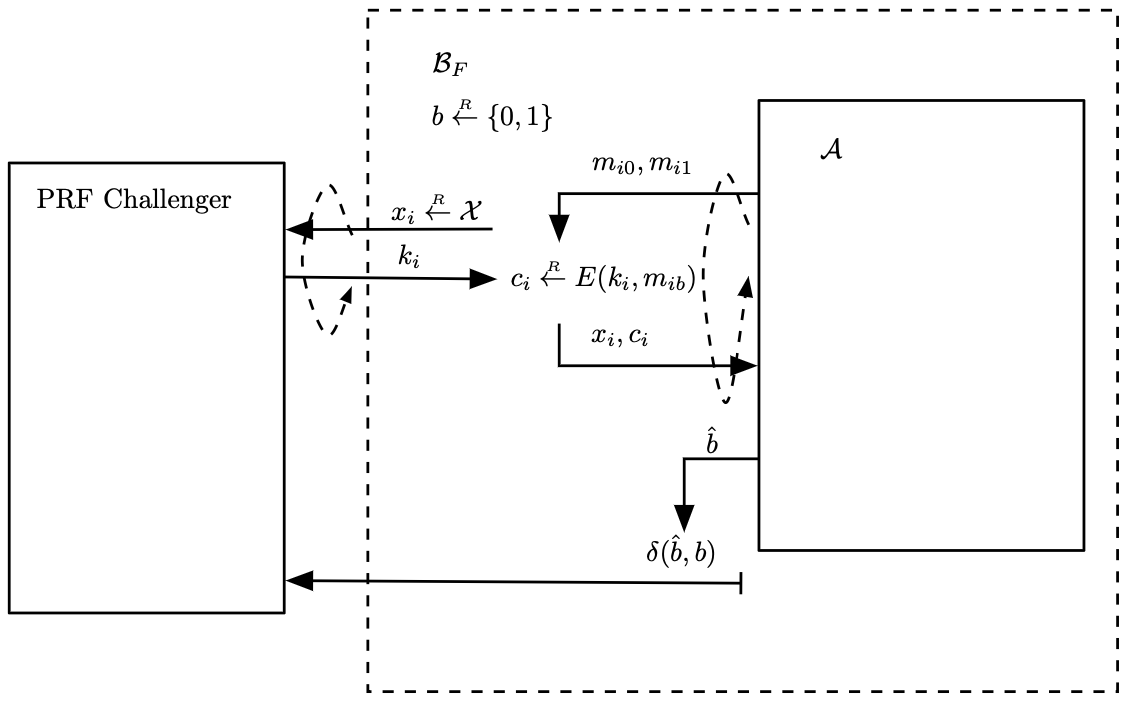
\includegraphics[width=0.8\linewidth]{figures/chapter5/fig1.png}
%  \caption{定理 \ref{theo:5-2} 的证明中的对手 $\mathcal{B}_F$}
%  \label{fig:5-1}
%\end{figure}

\begin{figure}
  \centering
  \input{figures/chapter5/fig1.tex}
  \caption{定理 \ref{theo:5-2} 的证明中的对手 $\mathcal{B}_F$}
  \label{fig:5-1}
\end{figure}

\vspace{5pt}

\noindent\textbf{游戏$\mathbf{2}$}。
接下来,我们使用我们的``忠实的侏儒"的思路(见 \ref{subsec:4-4-2} 小节)来实现随机函数 $f$。我们的``侏儒"必须跟踪 $f$ 的输入,并检测相同的输入是否被使用了两次。在下面的逻辑中,我们的``侏儒"使用一个真随机值作为 $k_i$ 的``默认"值,但如果有必要的话,这个值也可以被覆写,就像标有 ($*$) 的那一行所示:

\vspace{5pt}

\hspace*{5pt} 选取 $b\overset{\rm R}\leftarrow\{0,1\}$\\
\hspace*{26pt} 对于 $i=1,\dots,Q$:\\
\hspace*{50pt} 选取 $x_i\overset{\rm R}\leftarrow\mathcal{X}$\\
\hspace*{50pt} 计算 $k_i\leftarrow\mathcal{K}$\\
\hspace*{3pt} ($*$)
\hspace*{26.5pt} 如果存在某个 $j<i$ 使得 $x_i=x_j$,就令 $k_i\leftarrow k_j$\\
\hspace*{26pt} 当收到第 $i$ 个查询 $(m_{i0},m_{i1})\in\mathcal{M}^2$ 时:\\
\hspace*{50pt} 计算 $c_i\overset{\rm R}\leftarrow E(k_i,m_{ib})$\\
\hspace*{50pt} 将 $(x_i,c_i)$ 发送给对手。

\vspace{5pt}

\noindent
由于这是对随机函数 $f$ 的忠实实现,我们有:
\begin{equation}\label{eq:5-9}
\Pr[W_2]=\Pr[W_1]
\end{equation}

\noindent\textbf{游戏$\mathbf{3}$}。
接下来,我们让我们的侏儒变得``健忘",只需要丢掉上一个游戏中标有 ($*$) 的那一行:

\vspace{5pt}

\hspace*{5pt} 选取 $b\overset{\rm R}\leftarrow\{0,1\}$\\
\hspace*{26pt} 对于 $i=1,\dots,Q$:\\
\hspace*{50pt} 选取 $x_i\overset{\rm R}\leftarrow\mathcal{X}$\\
\hspace*{50pt} 计算 $k_i\leftarrow\mathcal{K}$\\
\hspace*{26pt} 当收到第 $i$ 个查询 $(m_{i0},m_{i1})\in\mathcal{M}^2$ 时:\\
\hspace*{50pt} 计算 $c_i\overset{\rm R}\leftarrow E(k_i,m_{ib})$\\
\hspace*{50pt} 将 $(x_i,c_i)$ 发送给对手。

\vspace{5pt}

为了分析 $|\Pr[W_3]-\Pr[W_2]|$ 的值,我们使用差分引理(定理 \ref{theo:4-7})。为此,我们将游戏 $2$ 和游戏 $3$ 视为运行在相同的基础概率空间上:对手和挑战者所做的随机选择在两个游戏中都是相同的,仅有的不同是挑战者计算应答的规则。特别地,两个游戏中的变量 $x_i$ 都是相同的。我们定义 $Z$ 为存在 $i\neq j$ 使得 $x_i=x_j$ 成立的事件。显然,除非 $Z$ 发生,否则游戏 $2$ 和游戏 $3$ 的流程是相同的;特别是,当且仅当 $W_3\land\bar{Z}$ 发生时,$W_2\land\bar{Z}$ 才会发生。因此,基于差分引理,我们有:
\begin{equation}\label{eq:5-10}
|\Pr[W_3]-\Pr[W_2]|\leq\Pr[Z]
\end{equation}
此外,不难发现:
\begin{equation}\label{eq:5-11}
\Pr[Z]\leq\frac{Q^2}{2N}
\end{equation}
这是因为 $Z$ 是小于 ${Q^2}/{2}$ 个事件的联合,其中每个事件发生的概率都是 ${1}/{N}$。

注意到,在游戏 $3$ 中,每条消息都使用独立的密钥 $k_i$ 来加密。所以接下来,我们打``语义安全牌",声称:
\begin{equation}\label{eq:5-12}
|\Pr[W_3]-{1}/{2}|={\rm MSS}\mathsf{adv}^*[\mathcal{\bar{B}}_\mathcal{E}, \mathcal{E}]
\end{equation}
其中,$\mathcal{\bar{B}}_\mathcal{E}$ 是一个有效对手,它就 $\mathcal{E}$ 进行攻击游戏 \ref{game:5-1} 的比特猜测版本,在该游戏中最多向其挑战者发起 $Q$ 次查询。

游戏 $3$ 语法很自然地为 $\mathcal{\bar{B}}_\mathcal{E}$ 的设计提供了灵感,它的工作方式如下:
\begin{quote}
$\mathcal{\bar{B}}_\mathcal{E}$ 扮演 $\mathcal{A}$ 的挑战者,在收到 $\mathcal{A}$ 的第 $i$ 个查询 $(m_{i0},m_{i1})$ 时,将 $(m_{i0},m_{i1})$ 提交给自己的挑战者,并得到一个密文 $c_i\in\mathcal{C}$。然后 $\mathcal{\bar{B}}_\mathcal{E}$ 从 $\mathcal{X}$ 中随机选择 $x_i$,并将 $(x_i,c_i)$ 发送给 $\mathcal{A}$ 作为对后者查询的应答。

当 $\mathcal{A}$ 最终输出一比特 $\hat{b}$ 时,$\mathcal{\bar{B}}_\mathcal{E}$ 也输出这个比特。
\end{quote}
对手 $\mathcal{\bar{B}}_\mathcal{E}$ 的工作原理见图 \ref{fig:5-2}。

%\begin{figure}
%  \centering
%  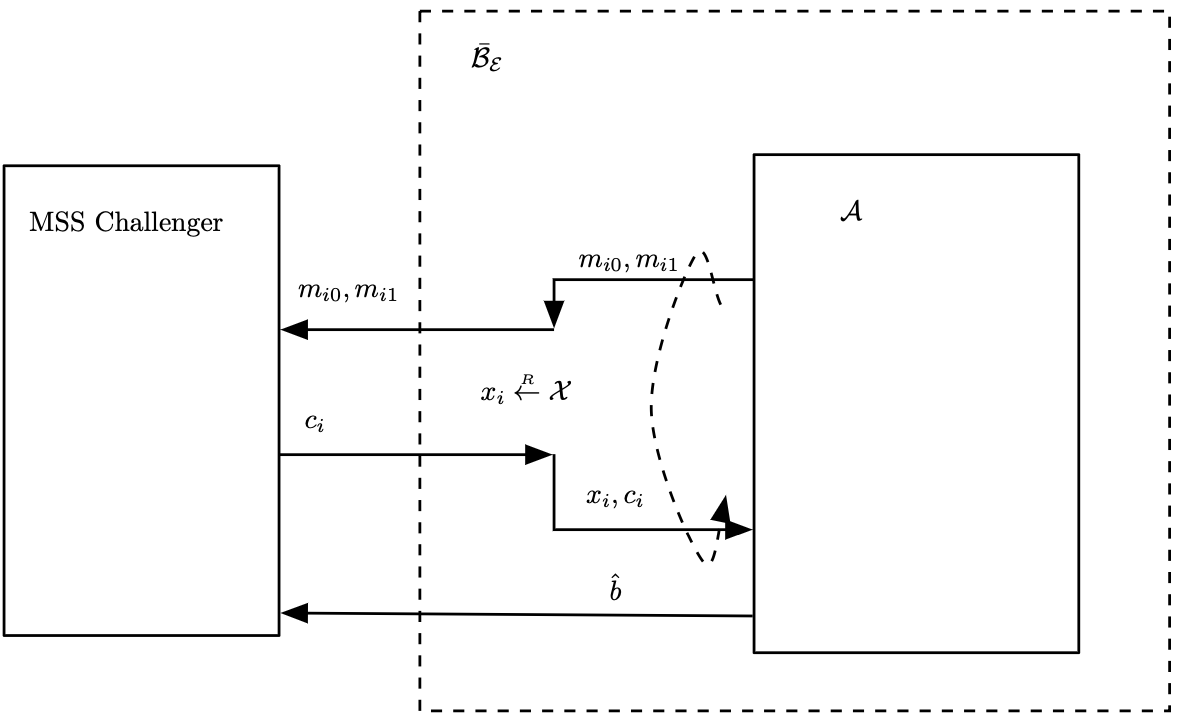
\includegraphics[width=0.8\linewidth]{figures/chapter5/fig2.png}
%  \caption{定理 \ref{theo:5-2} 的证明中的对手 $\mathcal{\bar{B}}_\mathcal{E}$}
%  \label{fig:5-2}
%\end{figure}

\begin{figure}
  \centering
  \input{figures/chapter5/fig2.tex}
  \caption{定理 \ref{theo:5-2} 的证明中的对手 $\mathcal{\bar{B}}_\mathcal{E}$}
  \label{fig:5-2}
\end{figure}

从构造(和式 \ref{eq:2-11})可以看出,式 \ref{eq:5-12} 显然成立。此外,根据定理 \ref{theo:5-1} 和式 \ref{eq:5-1},我们有:
\begin{equation}\label{eq:5-13}
{\rm MSS}\mathsf{adv}^*[\mathcal{\bar{B}}_\mathcal{E}, \mathcal{E}]=Q\cdot{\rm SS}\mathsf{adv}^*[\mathcal{B}_\mathcal{E},\mathcal{E}]
\end{equation}
其中 $\mathcal{B}_\mathcal{E}$ 是一个有效对手,它就 $\mathcal{E}$ 进行攻击游戏 \ref{game:2-1} 的比特猜测版本。

将式 \ref{eq:5-7} 到式 \ref{eq:5-13} 相结合,我们就可以得到式 \ref{eq:5-6}。另外,我们可以发现,$\mathcal{B}_F$ 和 $\mathcal{B}_\mathcal{E}$ 的运行时间与 $\mathcal{A}$ 的运行时间大致相同;事实上,它们都是围绕 $\mathcal{A}$ 的基本包装器,无论 $\mathcal{A}$ 是否是有效的,式 \ref{eq:5-5} 都是成立的。
\end{proof}

虽然上面的证明有点长,但我们希望读者认识到它实际上是很自然的,而且所有的步骤都相当容易掌握。另外,这个证明还说明了在设计一个安全证明时,我们如何引入一个以上的安全假设,并将安全证明设计成一连串的游戏。

\begin{remark}\label{remark:5-2}
我们简单提一下,即使构造中所使用的 PRF $F$ 只是弱安全的(见定义 \ref{def:4-3}),定理 \ref{theo:5-2} 中的混合构造 $\mathcal{E}'$ 仍然是 CPA 安全的。为了在这个较弱的假设下证明定理 \ref{theo:5-2},注意到,在游戏 $0$ 和游戏 $1$ 中,挑战者只在 $\mathcal{X}$ 中的\emph{随机}点上评估 PRF。因此,即使 $F$ 只是弱安全的,对手区分游戏 $0$ 和 $1$ 的优势也是可忽略不计的。
\end{remark}

\subsection{随机化计数器模式}\label{subsec:5-4-2}

我们可以直接从一个安全的 PRF 中构建一个 CPA 安全的密码,如下所示。假设 $F$ 是一个定义在 $(\mathcal{K},\mathcal{X},\mathcal{Y})$ 上的 PRF。我们假设 $\mathcal{X}=\{0,\dots,N-1\}$,并且 $\mathcal{Y}=\{0,1\}^n$。

对于任意多项式边界的 $\ell\geq1$,我们定义一个密码 $\mathcal{E}=(E,D)$,其密钥空间为 $\mathcal{K}$,消息空间为 $\mathcal{Y}^{\leq\ell}$,密文空间为 $\mathcal{X}\times\mathcal{Y}^{\leq\ell}$,如下所示:
\begin{itemize}
	\item 对于 $k\in\mathcal{K}$ 和 $m\in\mathcal{Y}^{\leq\ell}$,记 $v:=|m|$,我们定义:
	
	\hspace*{20pt} $E(k,m):=$\\
	\hspace*{50pt} 选取 $x\overset{\rm R}\leftarrow\mathcal{X}$\\
	\hspace*{50pt} 按如下方式计算 $c\in\mathcal{Y}^v$:\\
	\hspace*{75pt} 对于 $j=0,1,\dots,v-1$:\\
	\hspace*{100pt} 令 $c[j]\leftarrow F(k,\,x+j\;\mathrm{mod}\;N)\oplus m[j]$\\
	\hspace*{50pt} 输出 $(x,c)$;
	\item 对于 $k\in\mathcal{K}$ 和 $c'=(x,c)\in\mathcal{X}\times\mathcal{Y}^{\leq\ell}$,记 $v:=|c|$,我们定义:
	
	\hspace*{20pt} $D(k,c'):=$\\
	\hspace*{50pt} 按如下方式计算 $m\in\mathcal{Y}^v$:\\
	\hspace*{75pt} 对于 $j=0,1,\dots,v-1$:\\
	\hspace*{100pt} 令 $m[j]\leftarrow F(k,\,x+j\;\mathrm{mod}\;N)\oplus c[j]$\\
	\hspace*{50pt} 输出 $m$。
\end{itemize}

这个密码构造很像我们在 \ref{subsec:4-4-4} 小节中介绍的从 PRF 中建立一个 PRG,进而得到的流密码。不同的是,我们现在不再向 $F$ 输入固定序列以派生出密钥流,而是从一个随机起点开始,递增地来获得 $F$ 的输入序列。密文中的 $x$ 部分通常被称为\textbf{初始值 (initial value, IV)}。

在实践中,我们通常使用分组密码的加密函数来实现这里的 $F$,其中 $\mathcal{X}=\mathcal{Y}=\{0,1\}^n$。我们很自然地可以将 $n$ 比特的序列视为 $\{0,\dots,2^n-1\}$ 范围内的一个整数。碰巧的是,在这个构造中,我们根本就不需要分组密码的解密函数。关于这种模式的说明,可见图 \ref{fig:5-3}。

不难验证 $\mathcal{E}$ 确实是一个(概率性)密码。另外,需要注意的是,$\mathcal{E}$ 的消息空间是可变长的,如果想要使用攻击游戏 \ref{game:5-2} 定义的 CPA 安全性,消息 $m\in\mathcal{Y}^{\leq\ell}$ 的长度应当是其自然长度 $|m|$。

%\begin{figure}[p!]
%  \centering
%  \subfigure[加密]{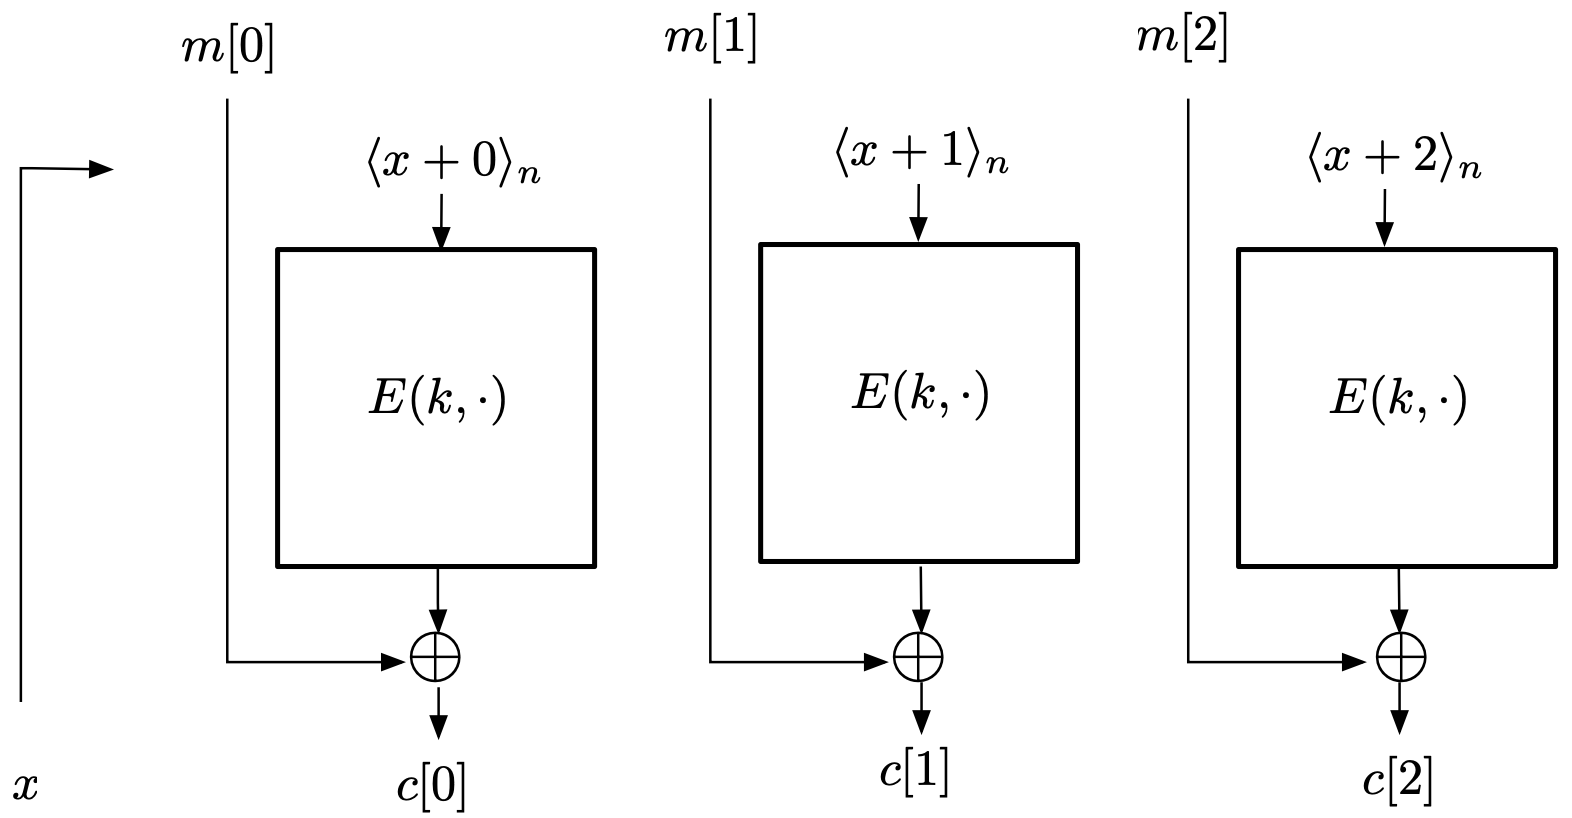
\includegraphics[width=0.65\linewidth]{figures/chapter5/fig3-a.png}}
%
%  \subfigure[解密]{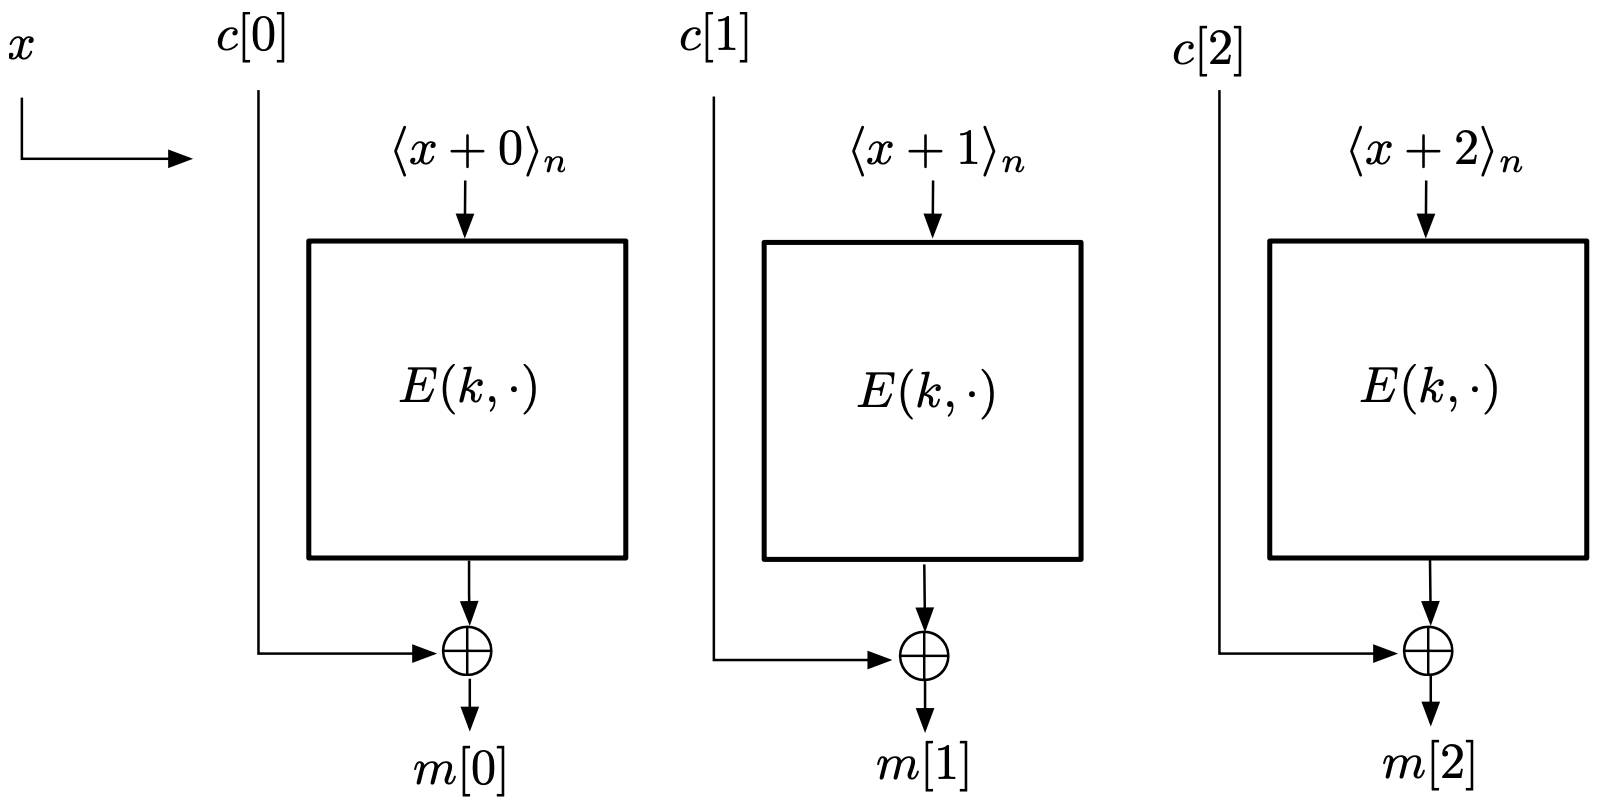
\includegraphics[width=0.65\linewidth]{figures/chapter5/fig3-b.png}}
%  \caption{随机化计数器模式($v=3$)}
%  \label{fig:5-3}
%\end{figure}

\begin{figure}
  \centering
  \subfigure[加密]{\input{figures/chapter5/fig3-a.tex}}
  
  \,
  
  \,
  
  \subfigure[解密]{\input{figures/chapter5/fig3-b.tex}}
  \caption{随机化计数器模式($v=3$)}
  \label{fig:5-3}
\end{figure}

\begin{theorem}\label{theo:5-3}
如果 $F$ 是一个安全的 PRF,并且 $N$ 是超多项式的,那么对于任何多项式约束的 $\ell\geq1$,上面描述的密码 $\mathcal{E}$ 都是一个 CPA 安全的密码。
\begin{quote}
特别地,对于每一个如攻击游戏 \ref{game:5-2} 中那样攻击 $\mathcal{E}$ 的 CPA 对手 $\mathcal{A}$,如果它最多能向其挑战者发起 $Q$ 次查询,则必然存在一个如攻击游戏 \ref{game:4-2} 中那样攻击 $F$ 的 PRF 对手 $\mathcal{B}$,其中 $\mathcal{B}$ 是一个围绕 $\mathcal{A}$ 的基本包装器,满足:
\end{quote}
\begin{equation}\label{eq:5-14}
{\rm CPA}\mathsf{adv}[\mathcal{A},\mathcal{E}]\leq\frac{2Q^2\ell}{N}+2\cdot{\rm PRF\mathsf{adv}}[\mathcal{B},F]
\end{equation}
\end{theorem}

\begin{proof}[证明思路]
假设我们从一个就 $\mathcal{E}$ 进行攻击游戏的对手开始。首先,利用 $F$ 是一个安全 PRF 的假设,我们可以有效地用一个真随机函数 $f$ 代替 $F$。其次,利用 $N$ 是超多项式的假设,以及每个 IV 都是随机选择的这一事实,我们可以认为,挑战者两次使用同一输入值评估 $f$ 的概率是可忽略不计的。但在这里,挑战者实际上是用一个独立的一次性密码本加密每条消息的,因此我们可以得出结论,对手在原始的 CPA 攻击游戏中的优势也是可忽略不计的。
\end{proof}

\begin{proof}
令 $\mathcal{A}$ 是一个有效对手,它就 $\mathcal{E}$ 进行攻击游戏 \ref{game:5-2},并且在该游戏中最多可以向其挑战者发起 $Q$ 次查询。我们想证明,如果 $F$ 是一个安全的 PRF,且 $N$ 是超多项式的,则 ${\rm CPA}\mathsf{adv}[\mathcal{A},\mathcal{E}]$ 可忽略不计。

不妨使用攻击游戏 \ref{game:5-2} 的比特猜测版本。我们需要证明,对于一个有效对手 $\mathcal{B}$,有:
\begin{equation}\label{eq:5-15}
{\rm CPA}\mathsf{adv}^*[\mathcal{A}, \mathcal{E}]\leq\frac{Q^2\ell}{N}+{\rm PRF\mathsf{adv}}[\mathcal{B},F]
\end{equation}
那么式 \ref{eq:5-14} 就可由式 \ref{eq:5-4} 得到。

这个证明的基本策略如下。首先,我们将游戏 $0$ 定义为 $\mathcal{A}$ 与其挑战者在攻击游戏 \ref{game:5-2} 的比特猜测版本中就 $\mathcal{E}$ 所进行的游戏。然后,我们再定义另外几个个游戏:游戏 $1$,游戏$2$ 和游戏 $3$。这些游戏都是在 $\mathcal{A}$ 和不同的挑战者之间进行的。在每个游戏中,我们用 $b$ 表示挑战者随机选择的比特,用 $\hat b$ 表示 $\mathcal{A}$ 输出的比特。我们想要证明,对于 $j = 1,\dots,3$,$|\Pr[W_j]-\Pr[W_{j-1}]|$ 的值都可忽略不计;此外,$\Pr[W_3]={1}/{2}$ 是显然成立的,继而我们可以得到 ${\rm CPA}\mathsf{adv}^*[\mathcal{A}, \mathcal{E}]:=|\Pr[W_0]-{1}/{2}|$ 也可忽略不计。

\vspace{5pt}

\noindent\textbf{游戏$\mathbf{0}$}。
我们可以将游戏 $0$ 中的挑战者描述如下:

\vspace{5pt}

\hspace*{5pt} 选取 $b\overset{\rm R}\leftarrow\{0,1\}$\\
\hspace*{26pt} 选取 $k'\overset{\rm R}\leftarrow\mathcal{K}$\\
\hspace*{26pt} 对于 $i=1,\dots,Q$:\\
\hspace*{50pt} 选取 $x_i\overset{\rm R}\leftarrow\mathcal{X}$\\
\hspace*{50pt} 对于 $j=0,\dots,\ell-1$:\\
\hspace*{75pt} 计算 $x_{ij}'\leftarrow x_i+j\mod N$\\
\hspace*{75pt} 计算 $y_{ij}\leftarrow F(k,x_{ij}')$\\
\hspace*{26pt} 当收到第 $i$ 个查询 $(m_{i0},m_{i1})$ 时,记 $v_i:=|m_{i0}|=|m_{i1}|$:\\
\hspace*{50pt} 按如下方法计算 $c_i\in\mathcal{Y}^{v_i}$:\\
\hspace*{75pt} 对于 $j=0,\dots,v_i-1$:\\
\hspace*{100pt} 计算 $c_i[j]\leftarrow y_{ij}\oplus m_{ib}[j]$\\
\hspace*{50pt} 将 $(x_i,c_i)$ 发送给对手。

\vspace{5pt}

根据构造,我们有:
\begin{equation}\label{eq:5-16}
{\rm CPA}\mathsf{adv}^*[\mathcal{A},\mathcal{E}]= |\Pr[W_0]-{1}/{2}|
\end{equation}

\noindent\textbf{游戏$\mathbf{1}$}。
接下来,我们打出我们的``PRF牌",用一个真随机函数 $f\in{\rm Funs}[\mathcal{X},\mathcal{Y}]$ 代替 $F(k,\cdot)$。在该游戏中,挑战者看起来是这样的:

\vspace{5pt}

\hspace*{5pt} 选取 $b\overset{\rm R}\leftarrow\{0,1\}$\\
\hspace*{26pt} 选取 $f\overset{\rm R}\leftarrow{\rm Funs}[\mathcal{X},\mathcal{Y}]$\\
\hspace*{26pt} 对于 $i=1,\dots,Q$:\\
\hspace*{50pt} 选取 $x_i\overset{\rm R}\leftarrow\mathcal{X}$\\
\hspace*{50pt} 对于 $j=0,\dots,\ell-1$:\\
\hspace*{75pt} 计算 $x_{ij}'\leftarrow x_i+j\mod N$\\
\hspace*{75pt} 计算 $y_{ij}\leftarrow f(x_{ij}')$\\
\hspace*{26pt} $\dots$

\vspace{5pt}

我们省略了挑战者的一部分代码,因为这些部分在所有游戏中都不会改变。我们声称:
\begin{equation}\label{eq:5-17}
|\Pr[W_1]-\Pr[W_0]|={\rm PRF}\mathsf{adv}[\mathcal{B},F]
\end{equation}
其中 $\mathcal{B}$ 是一个有效 PRF 对手;此外,由于我们假设 $F$ 是一个安全的 PRF,所以 ${\rm PRF}\mathsf{adv}[\mathcal{B},F]$ 一定是可忽略不计的。希望这(目前)已经是一个常规的论证,我们把具体的论证细节留给读者自行完成。

\vspace{5pt}

\noindent\textbf{游戏$\mathbf{2}$}。
接下来,我们用我们的``忠实的侏儒"的思路来实现随机函数 $f$。在描述我们的挑战者在这个游戏中的逻辑时,我们需要对索引数对 $(i,j)$ 使用标准词法排序;也就是说,当且仅当:
\[
i'<i
\quad\text{or}\quad
i'=i
\;\text{and}\;
j'<j
\]
时,我们记 $(i',j')<(i,j)$。在下面的逻辑中,我们的``侏儒"使用一个真随机值作为每个 $y_{ij}$ 的``默认"值,但如果有必要的话,这个值也可以被覆写,就像标有 ($*$) 的那一行所示:

\vspace{5pt}

\hspace*{5pt} 选取 $b\overset{\rm R}\leftarrow\{0,1\}$\\
\hspace*{26pt} 对于 $i=1,\dots,Q$:\\
\hspace*{50pt} 选取 $x_i\overset{\rm R}\leftarrow\mathcal{X}$\\
\hspace*{50pt} 对于 $j=0,\dots,\ell-1$:\\
\hspace*{75pt} 计算 $x_{ij}'\leftarrow x_i+j\mod N$\\
\hspace*{75pt} 计算 $y_{ij}\overset{\rm R}\leftarrow\mathcal{Y}$\\
\hspace*{3pt} ($*$)
\hspace*{51pt} 如果存在某个 $(i',j')<(i,j)$ 使得 $x_{ij}'=x_{i'j'}'$,则令 $y_{ij}\leftarrow y_{i'j'}$\\
\hspace*{26pt} $\dots$

\vspace{5pt}

由于这是对随机函数 $f$ 的忠实实现,我们有:
\begin{equation}\label{eq:5-18}
\Pr[W_2]=\Pr[W_1]
\end{equation}

\noindent\textbf{游戏$\mathbf{3}$}。
接下来,我们让我们的侏儒变得``健忘",只需要丢掉上一个游戏中标有 ($*$) 的那一行:

\vspace{5pt}

\hspace*{5pt} 选取 $b\overset{\rm R}\leftarrow\{0,1\}$\\
\hspace*{26pt} 对于 $i=1,\dots,Q$:\\
\hspace*{50pt} 选取 $x_i\overset{\rm R}\leftarrow\mathcal{X}$\\
\hspace*{50pt} 对于 $j=0,\dots,\ell-1$:\\
\hspace*{75pt} 计算 $x_{ij}'\leftarrow x_i+j\mod N$\\
\hspace*{75pt} 计算 $y_{ij}\overset{\rm R}\leftarrow\mathcal{Y}$\\
\hspace*{26pt} $\dots$

\vspace{5pt}

为了分析 $|\Pr[W_3]-\Pr[W_2]|$ 的值,我们使用差分引理(定理 \ref{theo:4-7})。为此,我们将游戏 $2$ 和游戏 $3$ 视为运行在相同的基础概率空间上:对手和挑战者所做的随机选择在两个游戏中都是相同的,仅有的不同是挑战者计算应答的规则。特别地,两个游戏中的变量 $x_{ij}'$ 都是相同的。我们定义 $Z$ 为存在某个 $(i',j')\neq(i,j)$ 使得 $x_{ij}'=x_{i'j'}'$ 成立的事件。显然,除非 $Z$ 发生,否则游戏 $2$ 和游戏 $3$ 的流程是相同的;特别是,当且仅当 $W_3\land\bar{Z}$ 发生时,$W_2\land\bar{Z}$ 才会发生。因此,基于差分引理,我们有:
\begin{equation}\label{eq:5-19}
|\Pr[W_3]-\Pr[W_2]|\leq\Pr[Z]
\end{equation}

我们声称:
\begin{equation}\label{eq:5-20}
\Pr[Z]\leq\frac{Q^2\ell}{N}
\end{equation}
为了证明这一声称,我们可以假设 $N\geq2\ell$(这一点无论如何都应该是普遍成立的,因为我们假设 $\ell	$ 是多项式边界的,$N$ 是超多项式的)。观察到,对于满足 $i\neq i'$ 的索引对 $i$ 和 $i'$,当且仅当:
\[
\{x_i,\dots,x_i+\ell-1\}
\;\cap\;
\{x_{i'},\dots,x_{i'}+\ell-1\}
\neq\varnothing
\]
成立时,事件 $Z$ 才会发生(算术运算是模 $N$ 的)。考虑任意固定的满足上述要求的一个数对 $(i,i')$。当以任意固定的 $x_i$ 为条件时,$x_i'$ 均匀分布在 $\{0,\dots,N-1\}$ 上,并且当且仅当:
\[
x_{i'}\in\{x_i+j\,:\,-\ell+1\leq j\leq\ell-1\}
\]
时,这些区间才会有重叠,这发生的概率是 ${2\ell-1}/{N}$,这样,由于我们有 ${Q(Q-1)}/{2}$ 种方法选择 $i$ 和 $i'$,所以式 \ref{eq:5-20} 成立。

最后,观察到,在游戏 $3$ 中,$y_{ij}$ 的值均匀独立分布在 $\mathcal{Y}$ 上,因此挑战者本质上是使用独立的一次性密码本来加密的。特别是,我们很容易看到,对手在这个游戏中的输出与 $b$ 无关,因此有:
\begin{equation}\label{eq:5-21}
\Pr[W_3]={1}/{2}
\end{equation}

将式 \ref{eq:5-16} 和 \ref{eq:5-21} 相结合,我们就可以得到式 \ref{eq:5-15},这就证明了本定理。
\end{proof}

\begin{remark}\label{remark:5-3}
我们可以把随机化计数器模式看作是 \ref{subsec:5-4-1} 小节中的通用混合构造的一个特例。参见联系 5.5。
\end{remark}

\subsubsection{案例研究:AES 计数器模式}

IPsec 协议使用 RFC 3686 中规定的 AES 计数器模式的一个特殊的变体。回顾一下,AES 使用 $128$ 比特长的分组。RFC 3686 不为每个消息随机挑选一个 $128$ 比特的 IV,而是按以下方式挑选 IV:
\begin{itemize}
	\item 最高的 $32$ 个有效比特是在生成密钥时随机选取的,并且在密钥的有效期内是固定的。这 $32$ 比特会用于所有使用该密钥加密的消息。
	\item 随后的 $64$ 比特是从 $\{0,1\}^{64}$ 中随机选出的。
	\item 最低的 $32$ 个有效比特均被置为 $1$。
\end{itemize}
通过这种方法产生的 $128$ 比特 IV 被用作计数器的初始值。在加密消息时,每加密一个消息分组,IV 的最低 $32$ 个有效比特就会递增一次。因此,可以加密的最大消息长度是 $2^{32}$ 个 AES 分组,即 $2^{36}$ 个字节。

通过这种 IV 的选择,解密者知道 IV 的最高 $32$ 个有效比特和最低 $32$ 个有效比特。因此,只有中间 $64$ 比特的 IV 需要和密文一起发送。

通过套用定理 \ref{theo:5-3} 的证明方法,我们同样可以证明这样选择 IV 是安全的。这种方法比随机选取 $128$ 位 IV 的微弱优势在于,本方法所产生的密文要更短一些。一个随机的 IV 会迫使加密器在密文中包含所有的 $128$ 个比特,而使用 RFC 3686 的方法,只需要 $64$ 比特,这就使密文缩小了 $8$ 个字节。

\subsection{密码分组链接模式}\label{subsec:5-4-3}

历史上的一个很重要的加密方法是在密码分组链接 (cipher block chaining, CBC) 模式下使用一个分组密码。这种方法被用在了 TLS 协议的旧版本中(比如 TLS 1.0)。它劣于下一节将要讨论的计数器模式加密。

令 $\mathcal{E}=(E,D)$ 是一个定义在 $(\mathcal{K},\mathcal{X})$ 上的分组密码,其中 $\mathcal{X}=\{0,1\}^n$。令 $N:=|\mathcal{X}|=2^n$。对于任意多项式边界的 $\ell\geq1$,我们定义一个密码 $\mathcal{E}'=(E',D')$,其密钥空间为 $\mathcal{K}$,消息空间为 $\mathcal{X}^{\leq\ell}$,密文空间为 $\mathcal{X}^{\leq\ell+1}\setminus\mathcal{X}^0$,即密文空间由最多包含 $\ell+1$ 个数据分组的所有非空序列构成。加密和解密的原理如下:
\begin{itemize}
	\item 对于 $k\in\mathcal{K}$ 和 $m\in\mathcal{X}^{\leq\ell}$,记 $v:=|m|$,我们定义:
	
	\hspace*{20pt} $E'(k,m):=$\\
	\hspace*{50pt} 按如下方式计算 $c\in\mathcal{Y}^{v+1}$:\\
	\hspace*{75pt} 选取 $c[0]\overset{\rm R}\leftarrow\mathcal{X}$\\
	\hspace*{75pt} 对于 $j=0,1,\dots,v-1$:\\
	\hspace*{100pt} 令 $c[j+1]\leftarrow E(k,\,c[j]\oplus m[j])$\\
	\hspace*{50pt} 输出 $c$;
	\item 对于 $k\in\mathcal{K}$ 和 $c\in\mathcal{X}^{\leq\ell+1}\setminus\mathcal{X}^0$,记 $v:=|c|-1$,我们定义:
	
	\hspace*{20pt} $D'(k,c):=$\\
	\hspace*{50pt} 按如下方式计算 $m\in\mathcal{Y}^{v}$:\\
	\hspace*{75pt} 对于 $j=0,1,\dots,v-1$:\\
	\hspace*{100pt} 令 $m[j]\leftarrow D(k,\,c[j+1])\oplus c[j]$\\
	\hspace*{50pt} 输出 $c$。
\end{itemize}

图 \ref{fig:5-4} 展示了 $|m|=3$ 情况下的加解密算法。这里,密文的第一项 $c[0]$ 也被称为初始值 IV。需要注意的是,和 \ref{subsec:5-4-2} 小节中介绍的计数器模式构造不同,在 CBC 模式中,我们必须使用分组密码,因为我们实际上需要使用分组密码的解密算法。

不难验证 $\mathcal{E}'$ 确实是一个(概率性)密码。另外,需要注意的是,$\mathcal{E}$ 的消息空间是可变长的,如果想要使用攻击游戏 \ref{game:5-2} 定义的 CPA 安全性,消息 $m\in\mathcal{X}^{\leq\ell}$ 的长度应当是其自然长度 $|m|$。

%\begin{figure}[p!]
%  \centering
%  \subfigure[加密]{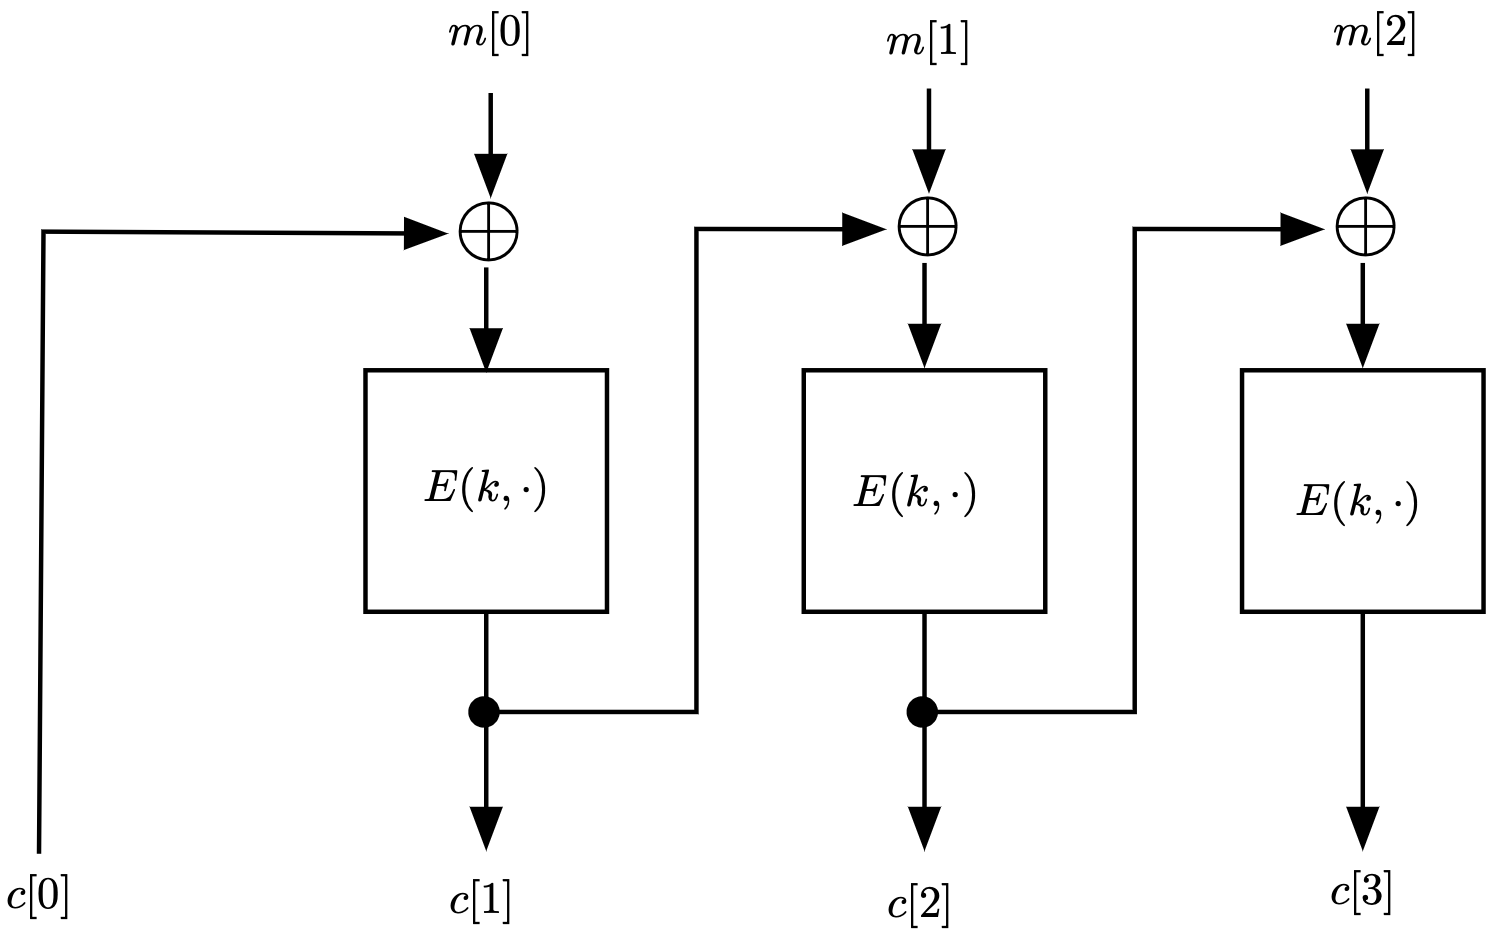
\includegraphics[width=0.65\linewidth]{figures/chapter5/fig4-a.png}}
%
%  \subfigure[解密]{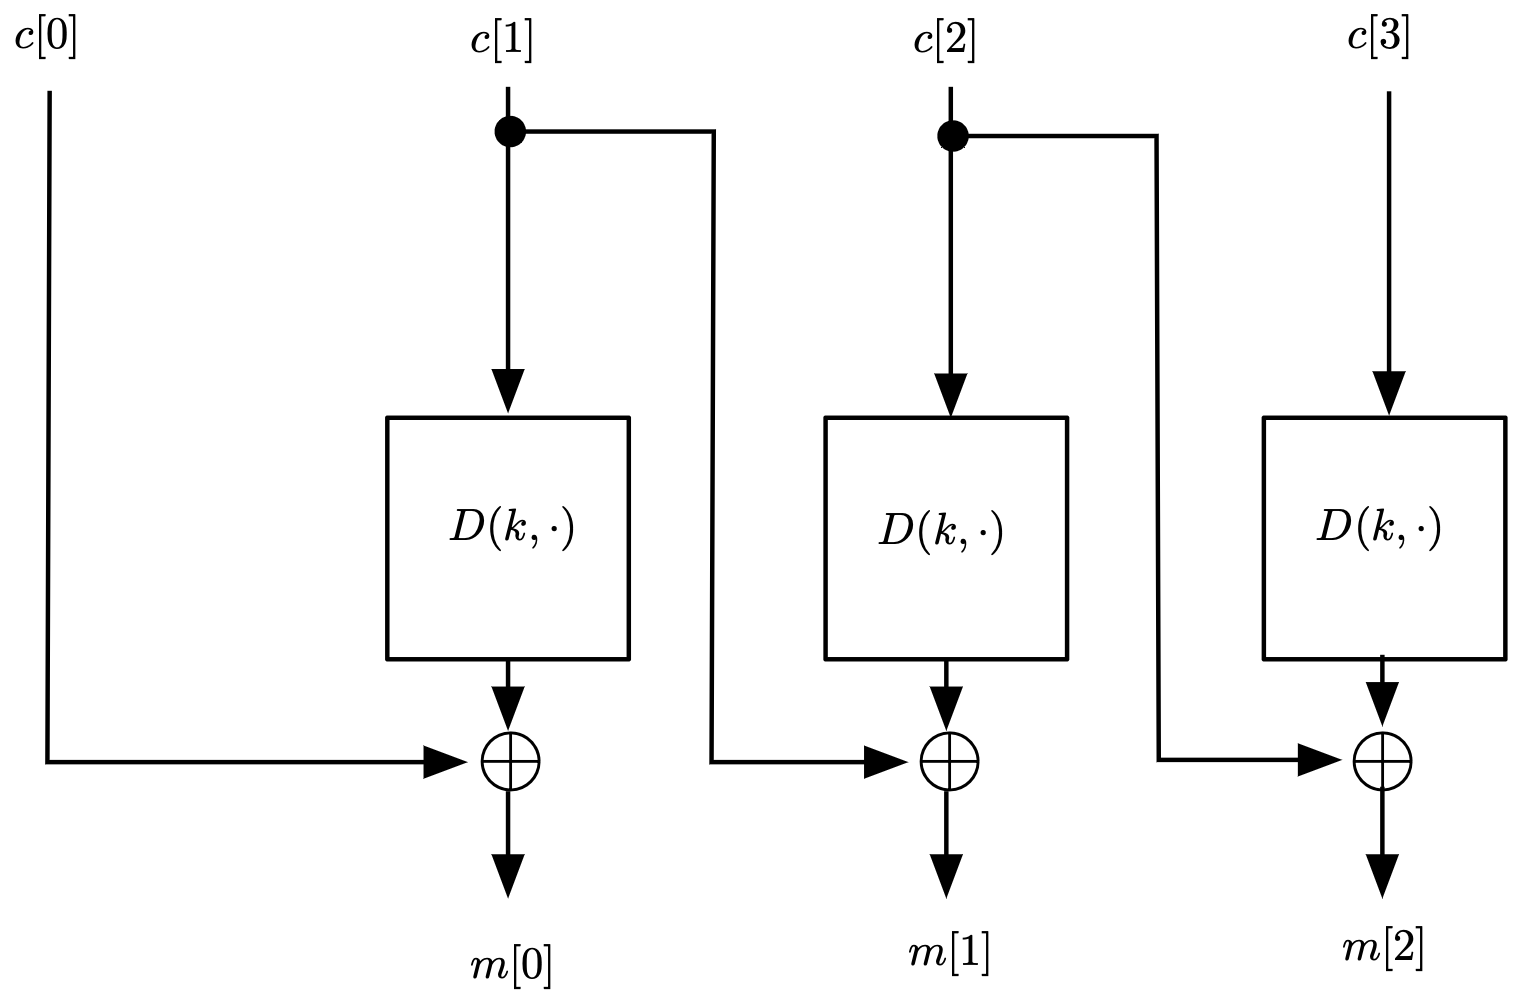
\includegraphics[width=0.65\linewidth]{figures/chapter5/fig4-b.png}}
%  \caption{$\ell=3$时CBC模式的加密和解密}
%  \label{fig:5-4}
%\end{figure}

\begin{figure}[p!]
  \centering
  \subfigure[加密]{\input{figures/chapter5/fig4-a.tex}}
  
  \,
  
  \,
  
  \subfigure[解密]{\input{figures/chapter5/fig4-b.tex}}
  \caption{$\ell=3$时CBC模式的加密和解密}
  \label{fig:5-4}
\end{figure}

\begin{theorem}\label{theo:5-4}
如果 $\mathcal{E}=(E,D)$ 是一个定义在 $(\mathcal{K},\mathcal{X})$ 上的安全的分组密码,并且 $N:=|\mathcal{X}|$ 是超多项式的,那么对于任何多项式约束的 $\ell\geq1$,上面描述的密码 $\mathcal{E}'$ 都是一个 CPA 安全的密码。
\begin{quote}
特别地,对于每一个如攻击游戏 \ref{game:5-2} 的比特猜测版本中那样攻击 $\mathcal{E}'$ 的 CPA 对手 $\mathcal{A}$,如果它最多能向其挑战者发起 $Q$ 次查询,则必然存在一个如攻击游戏 \ref{game:4-1} 中那样攻击 $\mathcal{E}$ 的 BC 对手 $\mathcal{B}$,其中 $\mathcal{B}$ 是一个围绕 $\mathcal{A}$ 的基本包装器,满足:
\end{quote}
\begin{equation}\label{eq:5-22}
{\rm CPA}\mathsf{adv}[\mathcal{A},\mathcal{E}']\leq\frac{2Q^2\ell^2}{N}+2\cdot{\rm BC\mathsf{adv}}[\mathcal{B},\mathcal{E}]
\end{equation}
\end{theorem}

\begin{proof}[证明思路]
证明的基本思路与定理 \ref{theo:5-3} 非常相似。我们从一个对 $\mathcal{E}'$ 进行 CPA 攻击游戏的对手开始,然后用一个真随机函数 $f$ 代替 $\mathcal{E}$。然后我们论证,挑战者两次使用同一输入值评估 $f$ 的概率是可忽略不计的。这样一来,挑战者看到的只是一堆随机比特,因此根本无法了解到关于加密消息的信息。
\end{proof}

\begin{proof}
假设 $\mathcal{A}$ 是一个有效的 CPA 对手,它按照攻击游戏 \ref{game:5-2} 攻击 $\mathcal{E}'$,且在该游戏中最多向其挑战者发起 $Q$ 次查询。我们想证明,如果 $\mathcal{E}$ 是一个安全的分组密码,并且 $N$ 是超多项式的,则 ${\rm CPA}\mathsf{adv}^*[\mathcal{A},\mathcal{E}]$ 是可忽略不计的。基于这些假设,根据推论 \ref{cor:4-5},加密函数 $E$ 是定义在 $(\mathcal{K},\mathcal{X},\mathcal{X})$ 上的一个安全的 PRF。

不妨使用攻击游戏 \ref{game:5-2} 的比特猜测版本。我们需要证明,对于一个有效对手 $\mathcal{B}$,有:
\begin{equation}\label{eq:5-23}
{\rm CPA}\mathsf{adv}^*[\mathcal{A}, \mathcal{E}']\leq\frac{Q^2\ell^2}{N}+{\rm BC\mathsf{adv}}[\mathcal{B},\mathcal{E}]
\end{equation}
那么式 \ref{eq:5-22} 就可由式 \ref{eq:5-4} 得到。

和之前一样,我们定义一连串的游戏:游戏 $0$,游戏 $1$,游戏 $2$ 和游戏 $3$。这些游戏都是在 $\mathcal{A}$ 和不同的挑战者之间进行的。游戏 $0$ 中的挑战者就是攻击游戏 \ref{game:5-2} 的比特猜测版本中就 $\mathcal{E}'$ 的挑战者。在每个游戏中,我们用 $b$ 表示挑战者随机选择的比特,用 $\hat b$ 表示 $\mathcal{A}$ 输出的比特。我们想要证明,对于 $j = 1,\dots,3$,$|\Pr[W_j]-\Pr[W_{j-1}]|$ 的值都可忽略不计;此外,$\Pr[W_3]={1}/{2}$ 是显然成立的,于是我们可以得到 ${\rm CPA}\mathsf{adv}^*[\mathcal{A}, \mathcal{E}']:=|\Pr[W_0]-{1}/{2}|$ 也可忽略不计。

\vspace{5pt}

\noindent\textbf{游戏$\mathbf{0}$}。
我们可以将游戏 $0$ 中的挑战者描述如下:

\vspace{5pt}

\hspace*{5pt} 选取 $b\overset{\rm R}\leftarrow\{0,1\}$\\
\hspace*{26pt} 选取 $k'\overset{\rm R}\leftarrow\mathcal{K}$\\
\hspace*{26pt} 当收到第 $i$ 个查询 $(m_{i0},m_{i1})$ 时,记 $v_i:=|m_{i0}|=|m_{i1}|$:\\
\hspace*{50pt} 按如下方法计算 $c_i\in\mathcal{X}^{v_i+1}$:\\
\hspace*{75pt} 选取 $c_i[0]\overset{\rm R}\leftarrow\mathcal{X}$\\
\hspace*{75pt} 对于 $j=0,\dots,v_i-1$:\\
\hspace*{100pt} 计算 $x_{ij}\leftarrow c_i[j]\oplus m_{ib}[j]$\\
\hspace*{100pt} 令 $c_i[j+1]\leftarrow E(k,x_{ij})$\\
\hspace*{50pt} 将 $c_i$ 发送给对手。

\vspace{5pt}

根据构造,我们有:
\begin{equation}\label{eq:5-24}
{\rm CPA}\mathsf{adv}^*[\mathcal{A},\mathcal{E}']= |\Pr[W_0]-{1}/{2}|
\end{equation}


\noindent\textbf{游戏$\mathbf{1}$}。
接下来,我们打出``PRF牌",用一个真随机函数 $f\in{\rm Funs}[\mathcal{X},\mathcal{X}]$ 代替 $F(k,\cdot)$。我们的挑战者在该游戏中看起来是这样的:

\vspace{5pt}

\hspace*{5pt} 选取 $b\overset{\rm R}\leftarrow\{0,1\}$\\
\hspace*{26pt} 选取 $f\overset{\rm R}\leftarrow{\rm Funs}[\mathcal{X},\mathcal{X}]$\\
\hspace*{26pt} 当收到第 $i$ 个查询 $(m_{i0},m_{i1})$ 时,记 $v_i:=|m_{i0}|=|m_{i1}|$:\\
\hspace*{50pt} 按如下方法计算 $c_i\in\mathcal{X}^{v_i+1}$:\\
\hspace*{75pt} 选取 $c_i[0]\overset{\rm R}\leftarrow\mathcal{X}$\\
\hspace*{75pt} 对于 $j=0,\dots,v_i-1$:\\
\hspace*{100pt} 计算 $x_{ij}\leftarrow c_i[j]\oplus m_{ib}[j]$\\
\hspace*{100pt} 令 $c_i[j+1]\leftarrow f(x_{ij})$\\
\hspace*{50pt} 将 $c_i$ 发送给对手。

\vspace{5pt}

我们声称:
\begin{equation}\label{eq:5-25}
|\Pr[W_1]-\Pr[W_0]|={\rm PRF}\mathsf{adv}[\mathcal{B},E]
\end{equation}
其中 $\mathcal{B}$ 是一个有效 PRF 对手;此外,由于我们假设 $F$ 是一个安全的 PRF,且 $N$ 是超多项式的,所以 ${\rm PRF}\mathsf{adv}[\mathcal{B},E]$ 一定是可忽略不计的。希望这(目前)已经是一个常规的论证,我们把具体的论证细节留给读者自行完成。

\vspace{5pt}

\noindent\textbf{游戏$\mathbf{2}$}。
相信读者应该已经知道我们下一步想要干什么了:我们用一个``忠实的侏儒"来实现随机函数 $f$。为此,我们引入一个随机值 $y_{ij}$ 来作为 $c_i[j]$ 的``默认"值,但如果有必要的话,这个值也可以被覆写,就像标有 ($*$) 的那一行所示:

\vspace{5pt}

\hspace*{5pt} 选取 $b\overset{\rm R}\leftarrow\{0,1\}$\\
\hspace*{26pt} 对于 $i=1,\dots,Q$ 和 $j=0,\dots,\ell$:\\
\hspace*{50pt} 设置 $y_{ij}\overset{\rm R}\leftarrow\mathcal{X}$\\
\hspace*{26pt} 当收到第 $i$ 个查询 $(m_{i0},m_{i1})$ 时,记 $v_i:=|m_{i0}|=|m_{i1}|$:\\
\hspace*{50pt} 按如下方法计算 $c_i\in\mathcal{X}^{v_i+1}$:\\
\hspace*{75pt} 选取 $c_i[0]\leftarrow y_{i0}$\\
\hspace*{75pt} 对于 $j=0,\dots,v_i-1$:\\
\hspace*{100pt} 计算 $x_{ij}\leftarrow c_i[j]\oplus m_{ib}[j]$\\
\hspace*{100pt} 令 $c_i[j+1]\leftarrow y_{i(j+1)}$\\
\hspace*{3pt} ($*$)
\hspace*{76.5pt} 如果存在某个 $(i',j')<(i,j)$ 使得 $x_{ij}'=x_{i'j'}$,则令 $c_i[j+1]\leftarrow c_{i'}[j'+1]$\\
\hspace*{50pt} 将 $c_i$ 发送给对手。

\vspace{5pt}

我们显然有:
\begin{equation}\label{eq:5-26}
\Pr[W_2]=\Pr[W_1]
\end{equation}

\noindent\textbf{游戏$\mathbf{3}$}。
接下来,我们让我们的侏儒变得``健忘",只需要丢掉标有 ($*$) 的那一行中的检查:

\vspace{5pt}

\hspace*{5pt} 选取 $b\overset{\rm R}\leftarrow\{0,1\}$\\
\hspace*{26pt} 对于 $i=1,\dots,Q$ 和 $j=0,\dots,\ell$:\\
\hspace*{50pt} 设置 $y_{ij}\overset{\rm R}\leftarrow\mathcal{X}$\\
\hspace*{26pt} 当收到第 $i$ 个查询 $(m_{i0},m_{i1})$ 时,记 $v_i:=|m_{i0}|=|m_{i1}|$:\\
\hspace*{50pt} 按如下方法计算 $c_i\in\mathcal{X}^{v_i+1}$:\\
\hspace*{75pt} 选取 $c_i[0]\leftarrow y_{i0}$\\
\hspace*{75pt} 对于 $j=0,\dots,v_i-1$:\\
\hspace*{100pt} 计算 $x_{ij}\leftarrow c_i[j]\oplus m_{ib}[j]$\\
\hspace*{100pt} 令 $c_i[j+1]\leftarrow y_{i(j+1)}$\\
\hspace*{50pt} 将 $c_i$ 发送给对手。

\vspace{5pt}

为了分析 $|\Pr[W_3]-\Pr[W_2]|$ 的值,我们使用差分引理(定理 \ref{theo:4-7})。为此,我们将游戏 $2$ 和游戏 $3$ 视为运行在相同的基础概率空间上:对手和挑战者所做的随机选择在两个游戏中都是相同的,仅有的不同是挑战者计算应答的规则。

我们定义 $Z$ 为存在 $x_{ij}'=x_{i'j'}$ 在游戏 $3$ 中成立的事件。注意到,事件 $Z$ 是以游戏 $3$ 中的 $x_{ij}$ 值来定义的。事实上,$x_{ij}$ 的值在游戏 $2$ 和游戏 $3$ 中的计算方式可能不一样,所以我们明确地以游戏 $3$ 中的值来定义事件 $Z$。显然,除非 $Z$ 发生,否则游戏 $2$ 和游戏 $3$ 的流程是相同的;特别是,当且仅当 $W_3\land\bar{Z}$ 发生时,$W_2\land\bar{Z}$ 才会发生。因此,基于差分引理,我们有:
\begin{equation}\label{eq:5-27}
|\Pr[W_3]-\Pr[W_2]|\leq\Pr[Z]
\end{equation}

我们声称:
\begin{equation}\label{eq:5-28}
\Pr[Z]\leq\frac{Q^2\ell}{2N}
\end{equation}
为了证明这一点,我们用 $Coins$ 来表示 $\mathcal{A}$ 做出的随机选择。观察到在游戏 $3$ 中,下面的几个值:
\[
Coins,\quad
b,\quad
y_{ij}\;(i=1,\dots,Q,\;j=0,\dots,\ell)
\]
是独立分布的。

考虑任意固定索引 $i=1,\dots,Q$。我们以 $Coins$,$b$ 和 $y_{i'j}$ 的任意固定值作为条件,其中 $i'=1,\dots,i-1$,$j=0,\dots,\ell$。在这个条件概率空间中,$m_{i0}$,$m_{i1}$ 和 $v_i$ 的值是完全确定的,对于 $i'=1,\dots,i-1$ 和 $j=0,\dots,v_{i'-1}$,$v_{i'}$ 和 $x_{i'j}$ 的值也是如此。然而,$y_{i0},\dots,y_{i\ell}$ 的值仍独立且均匀地分布在 $\mathcal{X}$ 上。此外,因为对于 $j=0,\dots,v_i-1$,我们有 $x_{ij}=y_{ij}\oplus m_{ib}[j]$,可知这些 $x_{ij}$ 也均匀独立分布在 $\mathcal{X}$ 上。因此,对于任意固定索引 $j=0,\dots,v_i-1$ 以及满足 $(i',j')<(i,j)$ 的固定索引 $i'$ 和 $j'$,$x_{ij}=x_{i'j'}$ 在上述条件概率空间中成立的概率为 ${1}/{N}$。因此,我们就可以通过一个简单的计算得到式 \ref{eq:5-28}。

最后,我们声称:
\begin{equation}\label{eq:5-29}
\Pr[W_3]={1}/{2}
\end{equation}
这是因为:
\[
Coins,\quad
b,\quad
y_{ij}\;(i=1,\dots,Q,\;j=0,\dots,\ell)
\]
是独立分布的,且对手的输出 $\hat{b}$ 是:
\[
Coins,\quad
y_{ij}\;(i=1,\dots,Q,\;j=0,\dots,\ell)
\]
的一个函数。由此我们可以看到,$\hat b$ 和 $b$ 是相互独立的,于是我们立即就可以得到式 \ref{eq:5-29}。

将式 \ref{eq:5-24} 和式 \ref{eq:5-29} 结合,我们就有:
\[
{\rm CPA}\mathsf{adv}^*[\mathcal{A}, \mathcal{E}']\leq\frac{Q^2\ell^2}{2N}+{\rm PRF\mathsf{adv}}[\mathcal{B},E]
\]
根据定理 \ref{theo:4-4},我们有:
\[
\big\lvert
{\rm BC\mathsf{adv}}[\mathcal{B},\mathcal{E}]-{\rm PRF\mathsf{adv}}[\mathcal{B},E]
\big\rvert
\leq\frac{Q^2\ell^2}{2N}
\]
这样就可以得到式 \ref{eq:5-23},于是该定理得证。
\end{proof}

\subsection{案例研究:TLS 1.0 中的 CBC 填充法}\label{subsec:5-4-4}

令 $\mathcal{E}=(E,D)$ 是一个领域为 $\mathcal{X}$ 的分组密码。我们对使用 $\mathcal{E}$ 的 CBC 模式加密的描述假定要加密的消息都是$\mathcal{X}^{\leq\ell}$ 中的元素。当领域是 $\mathcal{X}=\{0,1\}^{128}$ 时,就像 AES 的情况那样,这意味着我们只能加密那些长度为 $16$ 字节的倍数的消息。但是如果消息的长度并不是分组大小的整数倍,该怎么办呢?

现在,假设我们想用 CBC 模式的 AES 来加密一个 $v$ 字节的消息 $m$,而 $v$ 不一定是 $16$ 的倍数。我们首先想到的是对 $m$ 进行填充,使其长度为 $16$ 的倍数。显然,填充函数必须是可逆的,这是为了让我我们能在解密过程中移除填充。

TLS 1.0 协议定义了以下填充函数,用于在 CBC 模式下用 AES 加密一个 $v$ 字节的消息:令 $p:=16-(v\;\mathrm{mod}\;16)$,然后将 $p$ 字节的内容附加到消息 $m$ 后,且每个字节的内容都是 $p-1$。比如说,我们现在考虑以下两种情况:
\begin{itemize}
	\item 如果 $m$ 的长度是 $29$ 字节,那么 $p = 3$,此时填充由长度为 $3$ 个字节的消息 ``$222$" 组成,这样,填充后的消息长为 $32$ 字节,正好是两个 AES 分组。
	\item 如果 $m$ 的长度是分组大小的整数倍,比如 $32$ 字节,则 $p = 16$,那么填充就由 $16$ 字节组成。这样,填充后的消息长为 $48$ 字节,也就是三个 AES 分组。
\end{itemize}
即使消息长度是分组长度的整数倍,我们仍然需要在最后添加一个完整的假分组,这看起来好像很奇怪。但这是必要的,因为我们要保证解密程序能够正确地移除填充。基于上述设计,无论消息长度如何,填充方法都是可逆的。

一个很容易证明的事实是,任何 CBC 模式加密的可逆填充方案都要基于一个安全的分组密码,它能够为任意长度的消息提供 CPA 安全性。

只要明文长于一个分组,CBC 模式的填充方案就可以用一种叫做\textbf{密文窃取 (ciphertext stealing)}的方法来避免。我们会在练习 \ref{exer:5-16} 中讨论密文窃取在CBC下的一个变体。当需要加密的消息短于一个分组长时,比如说单字节的消息,仍然是需要进行填充的。

\subsection{计数器模式和 CBC 模式的比较}\label{subsec:5-4-5}

在本节的最后,我们对计数器模式和 CBC 模式进行一个简单地比较。我们假设计数器模式是用一个 PRF $F$ 实现的,它能将 $n$ 比特分组映射到 $n$ 比特分组,而 CBC 模式是用一个 $n$ 比特的分组密码实现的。在这两种情况下,我们都假设消息空间由最多 $\ell$ 个 $n$ 比特数据分组组成。基于本节给出的几个安全定理,我们有如下约束:
\[
\begin{aligned}
{\rm CPA}\mathsf{adv}[\mathcal{A}, \mathcal{E}_{\rm ctr}]\leq\frac{4Q^2\ell}{2^n}+2\cdot{\rm PRF}\mathsf{adv}[\mathcal{B}_F,F]\\
{\rm CPA}\mathsf{adv}[\mathcal{A},\mathcal{E}_{\rm cbc}]\leq\frac{2Q^2\ell^2}{2^n}+2\cdot{\rm BC}\mathsf{adv}[\mathcal{B}_\mathcal{E},\mathcal{E}]
\end{aligned}
\]
这里,$\mathcal{A}$ 可以是任意向其挑战者发起最多 $Q$ 次查询的 CPA 对手,$\ell$ 是任何一条消息的最大长度(数据分组数量)。出于简化讨论的目的,我们在下面的叙述中会忽略 ${\rm PRF}\mathsf{adv}[\mathcal{B}_F,F]$ 和 ${\rm BC}\mathsf{adv}[\mathcal{B}_\mathcal{E},\mathcal{E}]$ 这两项。

我们立即就可以看到,计数器模式有一个可量化的安全优势。为了更具体的解释这一问题,我们不妨假设分组大小为 $n=128$,每条消息为 1 MB(即 $2^{23}$ 比特),因此 $\ell=2^{16}$ 个分组。如果我们想把对手的优势约束在 $2^{-32}$ 以下,那么对于计数器模式,我们最多可以加密 $Q=2^{39.5}$ 条消息,而对于 CBC 模式,我们最多只能加密 $2^{32}$ 条消息。一旦用一个给定的密钥加密了 $Q$ 条消息之后,我们就必须换一个新的密钥。因此,与 CBC 模式相比,计数器模式中的一个密钥可以用来安全地加密更多的消息。

但是需要注意的是,如果使用一个分组密码来实现 $F$,这种数量上的优势就会消失,因为根据 PRF 切换引理(定理 \ref{theo:4-4})中的误差项,我们此时也需要依赖 $\ell$ 的二次项。然而,对于一个定制的 PRF 来说,这种数量上的优势仍然是适用的。

与 CBC 模式相比,计数器模式还有以下几个优点:
\begin{itemize}
	\item \emph{并行化和流水线}。计数器模式的加解密都是很容易并行化的,而尽管 CBC 模式的解密是可以并行化的,但其加密必然是串行性的。当底层硬件能够并行地处理多条指令时,支持并行地模式能够大大改善性能,而现代处理器通常就是这样的。更重要的是,考虑一个支持流水线的分组密码的一轮的硬件实现,如英特尔对 AES-128 的实现。流水线化使多个加密指令能够在同一时间执行。像计数器模式这样支持并行化的模式能使流水线保持忙碌,而在 CBC 加密中,由于这种模式固有的串行性,流水线在大多时间是没有被充分使用的。因此,如果明文已经被加载到 L1 缓存中,那么英特尔 Haswell 处理器上的计数器模式加密能比 CBC 模式加密快 $7$ 倍左右。
	\item \emph{更短的密文长度}。对于非常短的消息,计数器模式的密文比 CBC 模式的密文要短得多。例如,考虑一个 $1$ 字节的明文(在SSH协议中加密单个按键时产生)。计数器模式的密文只需要一个分组加 $1$ 字节:那一分组为随机 IV,那 $1$ 字节为加密后的明文。相比之下,一个 CBC 密文是两个完整的分组。如果假设分组长度是 $128$ 比特的话,这将会导致每个 CBC 密文都包含 $15$ 个多余的字节。
	\item \emph{只需加密}。CBC 模式同时使用分组密码的加密算法和解密算法,而计数器模式只会使用加密算法,因而可以简化代码实现。
\end{itemize}

\begin{remark}\label{remark:5-4}
随机化计数器模式和 CBC 模式都需要一个随机 IV。一些密码库实际上让上层应用来提供这个 IV。如果上层应用不努力确保 IV 有足够的随机性,就可能会导致很多的问题。比如说,对于计数器模式,有必要使 IV 足够分散,以便相应的间隔不会重叠。事实上,这个属性对于它来说就足够了。然而,对于 CBC 模式,需求就更多了:它还要求 IV 是不可预测的,参见练习 \ref{exer:5-13}。

把 IV 留给上层应用来提供,实际上是\emph{基于 nonce 加密}的一个例子,我们将在接下来的 \ref{sec:5-5} 节中详细探讨。
\end{remark}
\section{基于nonce的加密}\label{sec:5-5}

到目前为止,我们看到的所有 CPA 安全的加密方案都会受到\emph{密文扩展 (ciphertext expansion)}的影响,即它们的密文都比明文要长。例如,\ref{subsec:5-4-1} 小节介绍的通用混合构造产生了密文 $(x,c)$,其中 $x$ 属于某个 PRF 的输入空间,$c$ 是对消息的加密;\ref{subsec:5-4-2} 小节中的计数器模式所产生的密文 $(x,c)$ 结构也很类似。同样,\ref{subsec:5-4-3} 小节中的 CBC 模式将 IV 作为密文的一部分。

对于非常长的消息来说,即使密文稍微长了一点,其实也无所谓。比方说,如果我们使用 AES 在计数器模式或 CBC 模式下加密一条 1 MB 的消息,密文也只被扩展了 $16$ 个字节,这个扩展率可能完全是可以接受的。然而,如果一条消息本身也只有 $16$ 个字节甚至更短,密文至少就是明文的两倍长。

坏消息是,对于任何 CPA 安全的加密方案来说,一定程度的密文扩展是不可避免的(见练习 \ref{exer:5-10})。好消息是,如果施加一些特殊条件,密文扩展也是可以绕过的。比方说,现在我们假设 Alice 和 Bob 是完全同步的,所以 Alice 首先发送 $m_1$ 的加密,然后发送 $m_2$ 的加密,以此类推。而 Bob 首先解密 $m_1$ 的加密,然后解密 $m_2$ 的加密,以此类推。更具体地说,假设 Alice 和 Bob 使用 \ref{subsec:5-4-1} 小节中的通用混合构造。回顾一下,在这种情况下,消息 $m_i$ 对应的密文是 $(x_i,c_i)$,其中 $c_i:=E(k_i,m_i)$,$k_i:=F(x_i)$。为了确保安全性,我们要求 $x_i$ 的值各不相同。当 Alice 和 Bob 完全同步时(即 Alice 发送的密文按顺序到达 Bob),他们只需要在 PRF $F$ 的输入空间上对一个由不同元素组成的固定序列 $x_1,x_2,\dots$ 达成一致。

加密方案的这种操作模式并不真正适合我们的框架。从历史上看,有两种方法可以修改框架以允许这种类型的操作。一种方法是允许\emph{有状态的}加密方案,即加密和解密算法都保持一些内部状态,它们随着算法的每次使用而变化。在上一段的例子中,该状态只包含一个计数器,它的值随着算法的每次使用而递增。这种方法要求加密器和解密器完全同步,这限制了它的适用性,我们不会进一步讨论它。

第二种,也是更流行的一种方法,被称为\emph{基于 nonce 的加密}。在这种方法中,加密和解密算法都没有内部状态,而是接受一个额外的输入 $\mathpzc{N}$,称为 \emph{nonce}。基于 nonce 加密的语法形如:
\[
c=E(k,m,{\scriptstyle\mathpzc{N}})
\]
其中 $c\in\mathcal{C}$ 是密文,$k\in\mathcal{K}$ 是密钥,$m\in\mathcal{M}$ 是消息,${\scriptstyle\mathpzc{N}}\in\mathpzc{N}$ 是一个 nonce。此外,我们要求加密算法 $E$ 是确定性的。同样地,解密的语法形如:
\[
m=D(k,c,{\scriptstyle\mathpzc{N}})
\]
其目的是,用特定的 nonce 加密的消息应该能用相同的 nonce 解密,而这取决于使用该加密方案的应用程序。更正式地说,正确性要求是:
\[
D(k,\;E(k,m,{\scriptstyle\mathpzc{N}}),\;{\scriptstyle\mathpzc{N}})=m
\]
对于任意的 $k\in\mathcal{K}$,$m\in\mathcal{M}$ 和 ${\scriptstyle\mathpzc{N}}\in\mathpzc{N}$ 都成立。我们称基于 nonce 的密码 $\mathcal{E}=(E,D)$ 定义在 $(\mathcal{K},\mathcal{M},\mathcal{C},\mathpzc{N})$ 上。

直观地说,如果一个基于 nonce 的加密方案不会向窃听者泄露任何有用的信息,那么它就是 CPA 安全的,前提是在加密过程中任意一个 nonce 都不会被重复使用。这同样也要由使用该加密方案的应用程序来保证。请注意,这个关于如何使用 nonce 的要求是非常弱的,比要求它们是不可预测的要弱得多,更不用说要求它们是随机选出的了。

通过略微修改 CPA 安全性的原始定义,我们很容易定义这一安全概念。

\begin{game}[基于 nonce 的 CPA 安全性]\label{game:5-3}
对于一个定义在 $(\mathcal{K},\mathcal{M},\mathcal{C},\mathpzc{N})$ 上的给定密码 $\mathcal{E}=(E,D)$ 和一个给定对手 $\mathcal{A}$,我们定义两个实验:实验$0$和实验$1$。对于$b=0,1$,我们定义:

\noindent\textbf{实验$b$:}
\begin{itemize}
	\item 挑战者选取 $k\overset{\rm R}\leftarrow\mathcal{K}$。
	\item 对手向挑战者发起一连串的查询。\\
	对于$i = 1,2,\dots$,第 $i$ 个查询是一对相同长度的消息 $m_{i0},m_{i1}\in\mathcal{M}$ 和一个 nonce ${\scriptstyle\mathpzc{N}}_i\in\mathpzc{N}\setminus\{{\scriptstyle\mathpzc{N}}_1,\dots,{\scriptstyle\mathpzc{N}}_{i-1}\}$。\\
	挑战者计算 $c_i\leftarrow E(k,m_{ib},{\scriptstyle\mathpzc{N}}_i)$,并将 $c_i$ 发送给对手。
	\item 对手输出一个比特 $\hat{b}\in\{0,1\}$。
\end{itemize}

对于 $b=0,1$,令 $W_b$ 是 $\mathcal{A}$ 在实验 $b$ 中输出 $1$ 的事件。 我们定义 $\mathcal{A}$ 就 $\mathcal{E}$ 的\textbf{优势}为:
\[
{\rm nCPA}\mathsf{adv}[\mathcal{A},\mathcal{E}]:=|\Pr[W_0]-\Pr[W_1]|
\]
\end{game}

请注意,在上述游戏中,nonce 完全在对手的控制之下,只受制于对它们每个元素都是唯一值的约束。

\begin{definition}[基于 nonce 的 CPA 安全性]\label{def:5-3}
如果对于所有有效对手 $\mathcal{A}$,${\rm nCPA}\mathsf{adv}[\mathcal{A},\mathcal{E}]$ 的值都可忽略不计,那么基于 nonce 的密码 $\mathcal{E}$ 就被称为\textbf{对选择明文攻击是语义安全(semantically secure against chosen plaintext attack, CPA secure)}的。
\end{definition}

如同在 \ref{subsec:2-2-5} 小节中那样,攻击游戏 \ref{game:5-3} 可以被重构为一个``比特猜测"游戏,我们有:
\begin{equation}\label{eq:5-30}
{\rm nCPA}\mathsf{adv}[\mathcal{A},\mathcal{E}]= 2\cdot{\rm nCPA}\mathsf{adv}^*[\mathcal{A},\mathcal{E}]
\end{equation}
其中${\rm nCPA}\mathsf{adv}^*[\mathcal{A},\mathcal{E}]:=|\Pr[\hat{b}=b]-{1}/{2}|$处于攻击游戏 \ref{game:5-3} 的一个挑战者只是随机选择 $b$ 的版本中。

\subsection{基于 nonce 的通用混合加密}\label{subsec:5-5-1}

让我们把 \ref{subsec:5-4-1} 小节介绍的通用混合构造重构为一个基于 nonce 的加密方案。与之前一样,我们假设 $\mathcal{E}$ 是一个定义在 $(\mathcal{K},\mathcal{M},\mathcal{C})$ 上的密码,并且坚持它是确定性的,且 $F$ 是一个定义在 $(\mathcal{K}',\mathcal{X},\mathcal{K})$ 上的 PRF。我们下面定义一个基于 nonce 的密码 $\mathcal{E}'$,它定义在 $(\mathcal{K}',\mathcal{M},\mathcal{C},\mathcal{X})$ 上:
\begin{itemize}
	\item 对于 $k'\in\mathcal{K}'$,$m\in\mathcal{M}$ 和 $x\in\mathcal{X}$,我们定义 $E'(k',m,x):=E(k,m)$,其中 $k:=F(k',x)$;
	\item 对于 $k'\in\mathcal{K}'$,$c\in\mathcal{C}$ 和 $x\in\mathcal{X}$,我们定义 $D'(k',c,x):=D(k,c)$,其中 $k:=F(k',x)$。
\end{itemize}
我们所做的只是把 $x\in\mathcal{X}$ 当作是一个 nonce;除此之外,该方案与 \ref{subsec:5-4-1} 小节中定义的方案完全相同。

不难验证 $\mathcal{E}'$ 满足正确性要求。此外,我们可以很容易地调整定理 \ref{theo:5-2} 的证明以证明下面的定理。

\begin{theorem}\label{theo:5-5}
如果 $F$ 是一个安全的 PRF,$\mathcal{E}$ 是一个语义安全的密码,则上面描述的密码 $\mathcal{E}'$ 是一个 CPA 安全的密码。
\begin{quote}
特别地,对于每个像攻击游戏 \ref{game:5-3} 的比特猜测版本那样攻击 $\mathcal{E}'$ 的 nCPA 对手 $\mathcal{A}$,假设它最多能向其挑战者发起 $Q$ 次查询,则必然存在一个像攻击游戏 \ref{game:4-2} 中那样攻击 $F$ 的 PRF 对手 $\mathcal{B}_F$,和一个像攻击游戏 \ref{game:2-1} 的比特猜测版本中那样攻击 $\mathcal{E}$ 的 SS 对手 $\mathcal{B}_\mathcal{E}$,其中 $\mathcal{B}_F$ 和 $\mathcal{B}_\mathcal{E}$ 都是围绕 $\mathcal{A}$ 的基本包装器,满足:
\end{quote}
\begin{equation}\label{eq:5-31}
{\rm nCPA}\mathsf{adv}[\mathcal{A},\mathcal{E}']\leq
2\cdot{\rm PRF}\mathsf{adv}[\mathcal{B}_F,F]+Q\cdot{\rm SS}\mathsf{adv}[\mathcal{B}_\mathcal{E},\mathcal{E}]
\end{equation}
\end{theorem}

我们把这个定理的证明留给读者作为练习。请注意,式 \ref{eq:5-5} 中的 ${Q^2}/{N}$ 项表示的是 $F$ 的输入发生碰撞的概率,这一项在式 \ref{eq:5-30} 中被删去了,这是因为根据定义,碰撞是不可能发生的。

\subsection{基于 nonce 的计数器模式}\label{subsec:5-5-2}

接下来,我们将 \ref{subsec:5-4-2} 小节中介绍的计数器模式密码重构为一个基于 nonce 的加密方案。作为一个初步的尝试,我们先简单地将该构造中的 $x\in\mathcal{X}$ 作为一个 nonce。

不幸的是,这个方案不能满足基于 nonce 的 CPA 安全性的定义。问题在于,攻击者可以选择两个不同的 nonce $x_1,x_2\in\mathcal{X}$ 使得区间 $\{x_1,\dots,x_1+\ell-1\}$ 和 $\{x_2,\dots,x_2+\ell-1\}$ 是有重叠的(同样,算术运算是模 $N$ 的)。在这种情况下,安全证明将被打破;事实上,我们很容易发起一个破坏性相当大的攻击,正如 \ref{sec:5-1} 节所讨论的,因为攻击者基本上可以迫使加密器重新使用``密钥流"中的一些相同比特。

幸运的是,解决这个问题不是很难。让我们假设 $\ell$ 能整除 $N$(在实践中,$\ell$和$N$都是$2$的整数次幂,所以这并不是一个问题)。然后,我们令 nonce 空间为 $\{0,\dots,{N}/{\ell}-1\}$,并将 nonce ${\scriptstyle\mathpzc{N}}$ 转换为 PRF 的输入 $x:={\scriptstyle\mathpzc{N}}\ell$。不难发现,对于任意两个不同的 nonce ${\scriptstyle\mathpzc{N}}_1$ 和 ${\scriptstyle\mathpzc{N}}_2$,对于 $x_1:={\scriptstyle\mathpzc{N}}_1\ell$ 和 $x_2:={\scriptstyle\mathpzc{N}}_2\ell$,区间 $\{x_1,\dots,x_1+\ell-1\}$ 和 $\{x_2,\dots,x_2+\ell-1\}$ 没有重叠。

有了这样修改后的 $\mathcal{E}$,我们可以很容易地调整定理 \ref{theo:5-3} 的证明,来证明下面的定理。

\begin{theorem}\label{theo:5-6}
如果 $F$ 是一个安全的 PRF,那么上面描述的基于 nonce 的密码 $\mathcal{E}$ 是一个 CPA 安全的密码。
\begin{quote}
特别地,对于每一个如攻击游戏 \ref{game:5-3} 中那样攻击 $\mathcal{E}$ 的 nCPA 对手 $\mathcal{A}$,必然存在一个如攻击游戏 \ref{game:4-2} 中那样攻击 $F$ 的 PRF 对手 $\mathcal{B}$,其中 $\mathcal{B}$ 是一个围绕 $\mathcal{A}$ 的基本包装器,满足:
\end{quote}
\begin{equation}\label{eq:5-32}
{\rm nCPA}\mathsf{adv}[\mathcal{A},\mathcal{E}]\leq2\cdot{\rm PRF\mathsf{adv}}[\mathcal{B},F]
\end{equation}
\end{theorem}

我们再次将该定理的证明留给读者作为练习。

\subsection{基于 nonce 的 CBC 模式}\label{subsec:5-5-3}

最后,我们考虑如何将 \ref{subsec:5-4-3} 小节中介绍的 CBC 模式加密方案重构为一个基于 nonce 的加密方案。作为一个初步的尝试,我们可以先简单地将 IV $c[0]$ 看作是一个 nonce。不幸的是,这并不能产生一个 CPA 安全的加密方案。在 nCPA 攻击游戏中,对手可以进行两次查询:

\vspace{5pt}

\hspace*{5pt} $(m_{10},m_{11},{\scriptstyle\mathpzc{N}}_1),$\\
\hspace*{26pt} $(m_{20},m_{21},{\scriptstyle\mathpzc{N}}_2)$

\vspace{5pt}

\noindent
其中:
\[
m_{10}={\scriptstyle\mathpzc{N}}_1\neq{\scriptstyle\mathpzc{N}}_2=m_{20},
\;\;
m_{11}=m_{21}
\]
这里,所有的消息都是单个分组的消息。在攻击游戏的实验 $0$ 中,产生的密文是相同的,而在实验 $1$ 中,密文是不同的。因此,我们可以完美地区分这两个实验。

同样,对它的修正也是很直接的。我们的想法是通过 PRF 将 nonce 映射为伪随机的 IV。因此,假设我们有一个定义在 $(\mathcal{K}',\mathpzc{N},\mathcal{X})$ 上的 PRF。这里,$F$ 的密钥空间 $\mathcal{K}'$ 和输入空间 $\mathpzc{N}$ 可以是任意的集合,但 $F$ 的输出空间 $\mathcal{X}$ 必须与底层的分组密码 $\mathcal{E}=(E,D)$ 的分组空间相匹配,即把后者定义在 $(\mathcal{K},\mathcal{X})$ 上。在基于 nonce 的 CBC 模式加密方案 $\mathcal{E}'$ 中,密钥空间是 $\mathcal{K}\times\mathcal{K}'$,在加密和解密算法中,IV 是由 nonce ${\scriptstyle\mathpzc{N}}$ 和密钥 $k'$ 计算出来的,即 $c[0]:=F(k',{\scriptstyle\mathpzc{N}})$。

有了这些修改,我们不难证明定理 \ref{theo:5-4} 的下述变体是成立的。

\begin{theorem}\label{theo:5-7}
如果 $\mathcal{E}=(E,D)$ 是一个定义在 $(\mathcal{K},\mathcal{X})$ 上的安全的分组密码,$N:=|\mathcal{X}|$ 是超多项式的,并且 $F$ 是一个定义在 $(\mathcal{K}',\mathpzc{N},\mathcal{X})$ 上的安全的 PRF,那么对于任何多项式约束的 $\ell\geq1$,上面描述的基于 nonce 的密码 $\mathcal{E}'$ 都是一个 CPA 安全的密码。
\begin{quote}
特别地,对于每一个如攻击游戏 \ref{game:5-3} 的比特猜测版本那样攻击 $\mathcal{E}'$ 的 nCPA 对手 $\mathcal{A}$,如果它最多能向其挑战者发起 $Q$ 次查询,则必然存在一个如攻击游戏 \ref{game:4-1} 那样攻击 $\mathcal{E}$ 的 BC 对手 $\mathcal{B}$ 和一个如攻击游戏 \ref{game:4-2} 那样攻击 $F$ 的 PRF 对手 $\mathcal{B}_F$,其中 $\mathcal{B}$ 和 $\mathcal{B}_F$ 都是 $\mathcal{A}$ 的基本包装器,满足:
\end{quote}
\begin{equation}\label{eq:5-33}
{\rm CPA}\mathsf{adv}[\mathcal{A},\mathcal{E}']\leq\frac{2Q^2\ell^2}{N}+2\cdot{\rm PRF\mathsf{adv}}[\mathcal{B}_F,F]+2\cdot{\rm BC\mathsf{adv}}[\mathcal{B},\mathcal{E}]
\end{equation}
\end{theorem}

同样,我们把定理的证明留给读者作为练习。请注意,在上述构造中,我们可以使用底层的分组密码 $\mathcal{E}$ 作为PRF $F$;但是,必须使用独立的密钥 $k$ 和 $k'$(见练习 \ref{exer:5-14})。

上面描述的基于 nonce 的 CBC 模式也被称为 \texttt{CBC-ESSIV}(加密盐扇区 IV),它被用于一些全盘加密系统,如\texttt{dm-crypt} 中。当对磁盘上的一个扇区进行加密时,扇区号被用作 nonce。其它的全盘加密系统使用可调整的加密方式,如练习 \ref{exer:4-11} 中所讨论的。
\section{一个有趣的应用:可撤销的广播加密}

电影公司花费大量精力制作大片,然后将电影(DVD)卖给数以百万计的客户,这些客户购买电影后就可以在家里观看它们。客户应该能够在一个没有网络连接的,无状态的独立电影播放器上观看电影。

然而,电影公司担心盗版问题,并不想把受版权保护的数字内容简单直接地以明文发送给数以百万计的用户。一个简单的解决方案是这样运行的。每个授权制造商都有一个\textbf{设备密钥} $k_\mathrm{d}\in\mathcal{K}$,它会把这个密钥嵌入到它所销售的每台设备中。如果有一百个授权设备制造商,那么就有一百个设备密钥 $k^{(1)}_\mathrm{d}, \dots, k^{(100)}_\mathrm{d}$。一部电影 $m$ 会被加密为:
\[
c_\mathrm{m}:=
\left\{
\begin{aligned}
& k\overset{\rm R}\leftarrow\mathcal{K}\\
& \text{for } i=1,\dots,100\;:\; c_i\leftarrow E(k^{(i)}_\mathrm{d},\,k)\\
& c\overset{\rm R}\leftarrow E'(k,m)\\
& \text{output } (c_1,\dots,c_{100},\;c)
\end{aligned}
\right\}
\]
其中 $(E,D)$ 是一个 CPA 安全的密码,并且在密钥空间为 $\mathcal{K}$ 的情况下,$(E',D')$ 是语义安全的。我们在练习 5.4 中分析了这个构造,我们在该练习中表明,这个构造是 CPA 安全的。我们将 $(c_1, \dots, c_{100})$ 称为密文头部,将 $c$ 称为密文体。

现在,每个授权设备都可以使用内嵌的设备密钥来解密电影。首先解密密文头部中适当的密文,然后使用获得的密钥 $k$ 来解密密文体。这种机制构成了用于加密 DVD 的\textbf{内容加扰系统(content scrambling system, CSS)}的基础。我们之前在 \ref{sec:3-8} 节中曾经遇到过 CSS。

这个方案的麻烦之处在于,一旦某一个设备被攻破,并且它的设备密钥 $k_\mathrm{d}$ 被提取并公布,那么任何人都可以用这个 $k_\mathrm{d}$ 来解密所有曾经发布过的电影。如果不破坏与之关联的许多消费者设备,就没有办法撤销 $k_\mathrm{d}$。事实上,这正是 CSS 被破解的方式:从某一台被授权的播放器中提取出设备密钥,然后使用一个名为 \textbf{DeCSS} 的系统解密被加密的 DVD。

从 CSS 中得到的教训是,全局不可撤销的设备密钥是一个很坏的主意。一旦单个密钥被泄露,所有的安全性都会丧失。当电影行业的硬件载体从 DVD 升级到蓝光时,它们获得了一次重新设计加密方案的机会。在这个被称为\textbf{高级访问内容系统 (Advanced Access Content System, AACS)} 的新方案中,每台设备都包含一个随机的设备密钥,且它对该设备是独一无二的。该系统的设计目标是支持数十亿台设备,并且让每台设备都有自己的密钥。

该系统的目标包含两个方面。首先,每个被授权的设备都应该能够解密每张蓝光光盘。第二,每当一个设备的密钥被提取和公布时,它应当可以被撤销,这使得这个设备的密钥不能被用来解密之后的蓝光光盘,但不会影响到任何其他的设备。

\begin{snote}[一个可撤销的广播系统。]
假设系统中有 $n$ 台设备,为了简单起见,我们假设 $n$ 是 $2$ 的整数次幂。我们把这 $n$ 台设备当作一个完全二叉树的叶子结点,如图 \ref{fig:5-5} 所示。二叉树上的每个结点都被分配了一个密钥空间 $\mathcal{K}$ 中的随机密钥。编号为 $i\in\{1,\dots,n\}$ 的设备中嵌入的密钥就是从编号为 $i$ 的叶子结点到根结点路径上所有密钥的集合。这样,每个设备都恰好被赋予了 $\log_2n$ 个 $\mathcal{K}$ 中的密钥。

当系统第一次启动时,还没有设备的密钥被撤销,所有的内容都是用根结点的密钥(图 \ref{fig:5-5} 中的编号为 $15$ 的密钥)加密的。更确切地说,一部电影 $m$ 会被加密为:
\[
c_\mathrm{m}:=
\left\{
\;
k\overset{\rm R}\leftarrow\mathcal{K},\;
c_1\overset{\rm R}\leftarrow E(k_\mathrm{root},\,k),\;
c\overset{\rm R}\leftarrow E'(k,m),\;
\text{output } (c_1,c)\;
\right\}
\]
因为所有设备都有根密钥 $k_\mathrm{root}$,所有设备都可以解密。
\end{snote}

%\begin{figure}
%  \centering
%  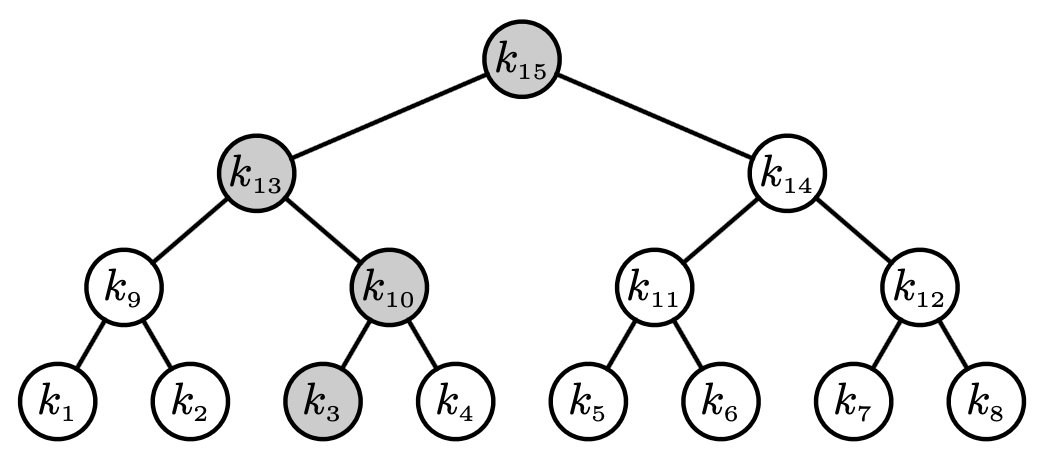
\includegraphics[width=0.45\linewidth]{figures/chapter5/fig5.png}
%  \caption{$n=8$个设备时的密钥树;被阴影标记的结点是嵌入设备 $3$ 中的密钥。}
%  \label{fig:5-5}
%\end{figure}

\begin{figure}
  \centering
  \input{figures/chapter5/fig5.tex}
  \caption{$n=8$个设备时的密钥树;被阴影标记的结点是嵌入设备 $3$ 中的密钥。}
  \label{fig:5-5}
\end{figure}

\begin{snote}[撤销设备。]
现在,假设编号为 $i$ 的设备被攻击,所有存储在它上面的密钥都被公开了。那么,所有以后的内容都应当使用与从 $i$ 号叶子结点到根结点的路径上的 $\log_2n$ 个结点的兄弟结点的关联密钥进行加密。比如说,当图 \ref{fig:5-5} 所示的 $3$ 号设备被撤销时,所有未来的内容都将会使用密钥 $k_4$,$k_9$ 和 $k_{14}$ 来进行加密,方法如下:
\begin{equation}\label{eq:5-34}
c_\mathrm{m}:=
\left\{
\begin{aligned}
& k\overset{\rm R}\leftarrow\mathcal{K}\\
& c_1\overset{\rm R}\leftarrow E(k_4,\,k),\;
c_2\overset{\rm R}\leftarrow E(k_9,\,k),\;
c_3\overset{\rm R}\leftarrow E(k_{14},\,k)\\
& c\overset{\rm R}\leftarrow E'(k,m)\\
& \text{output } (c_1,c_2,c_3,c)
\end{aligned}
\right\}
\end{equation}
同样,$(c_1,c_2,c_3)$ 是密文头部,$c$ 是密文体。请注意,$3$ 号设备现在无法解密 $c_\mathrm{m}$,因为它现在不能解密文头部中的任何一个密文。然而,其他每个设备都可以很容易地使用它所掌握的密钥之一进行解密。例如,$6$ 号设备可以使用 $k_{14}$ 来解密 $c_3$。事实上,如果像式 \ref{eq:5-34} 那样修改加密方案,我们就可以撤销 $3$ 号设备,同时又不对其他设备造成任何影响。但这样做的代价是,现在的密文头部包含了 $\log_2n$ 个分组,而在设备被撤销之前只有一个。

更一般地说,假设有 $r$ 个设备都被破坏了,因而需要撤销它们。令 $S\subseteq\{1,\dots,n\}$ 为未被破坏的设备的集合,那么有 $|S|=n-r$。新的内容将使用树中的密钥进行加密,因此 $S$ 中的设备可以解密,但 $S$ 之外的所有设备都无法解密。这样的密钥集可以使用下面的定义来描述。
\end{snote}

\begin{definition}\label{def:5-4}
令 $T$ 是一棵包含 $n$ 个叶子结点的完全二叉树,其中 $n$ 是$2$ 的整数次幂。令 $S\subseteq\{1,\dots,n\}$ 是一个由叶子结点组成的集合。对于一个结点集 $W\subseteq\{1,\dots,2n-1\}$,如果 $S$ 中的每个叶子结点都是 $W$ 中某个结点的后代,而 $S$ 之外的结点都不是的话,我们就称 $W$ \textbf{覆盖}了 $S$。我们用 $\mathrm{cover}(S)$ 来表示覆盖 $S$ 的最小结点集。
\end{definition}

图 \ref{fig:5-6} 展示了对叶子结点集 $\{1,2,4,5,6\}$ 的一个覆盖。该图的例子是 $3$、$7$ 和 $8$ 号设备被撤销的情况。显然,如果我们使用 $\mathrm{cover}(S)$ 中的密钥来加密一部电影 $m$,那么 $S$ 中的设备可以解密它,但 $S$ 外的设备不能。具体来说,我们加密 $m$ 的方法如下:
\begin{equation}\label{eq:5-35}
c_\mathrm{m}:=
\left\{
\begin{aligned}
& k\overset{\rm R}\leftarrow\mathcal{K}\\
& \text{for } u\in\mathrm{cover}(S)\;:\; c_u\overset{\rm R}\leftarrow E(k_u,\,k)\\
& c\overset{\rm R}\leftarrow E'(k,m)\\
& \text{output } (\{c_u\}_{u\in\mathrm{cover}(S)},\;c)
\end{aligned}
\right\}
\end{equation}
我们会在练习 5.21 中讨论该方案的安全性。

%\begin{figure}
%  \centering
%  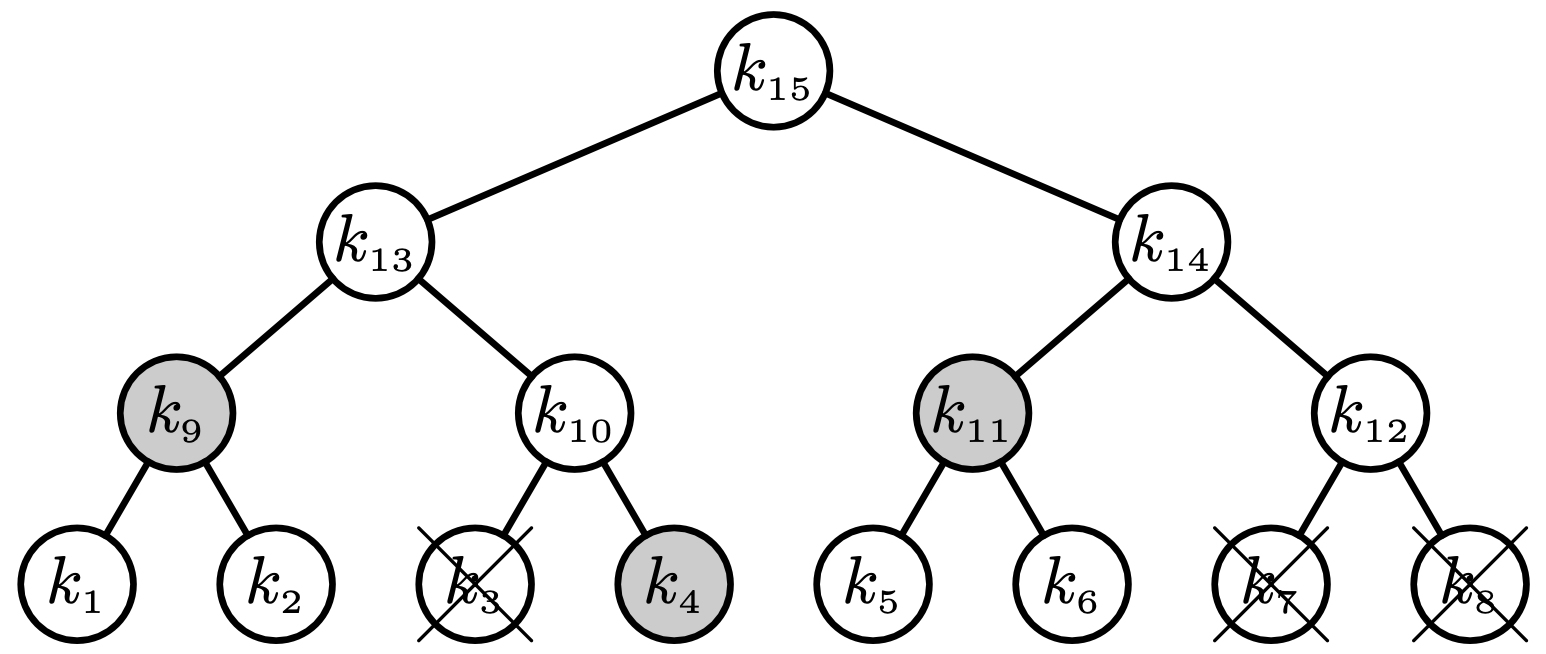
\includegraphics[width=0.45\linewidth]{figures/chapter5/fig6.png}
%  \caption{三个被阴影标记的结点是叶子集 $\{1,2,4,5,6\}$ 的最小覆盖。}
%  \label{fig:5-6}
%\end{figure}

\begin{figure}
  \centering
  \input{figures/chapter5/fig6.tex}
  \caption{三个被阴影标记的结点是叶子集 $\{1,2,4,5,6\}$ 的最小覆盖。}
  \label{fig:5-6}
\end{figure}

被撤销的设备越多,$c_\mathrm{m}$ 的密文头部就越大。下面的定理显示了在最坏的情况下密文头部会有多大。该证明是一个归纳论证,它还给出了一种用于计算最优覆盖的高效递归算法。

\begin{theorem}\label{theo:5-8}
令 $T$ 是一棵包含 $n$ 个叶子结点的完全二叉树,其中 $n$ 是$2$ 的整数次幂。对于每个 $1\leq r\leq n$ 以及每个包含 $n-r$ 个叶子结点的集合 $S$,我们都有:
\[
|\mathrm{cover}(S)|\leq r\cdot\log_2(n/r)
\]
\end{theorem}

\begin{proof}
我们通过在 $\log_2n$ 上的归纳法来证明该定理,当 $n=1$ 时,该定理显然成立。现在,假设该定理在有 $n/2$ 个叶子结点的树上成立,我们想要证明该定理在有 $n$ 个叶子结点的树 $T$ 上仍然成立。树 $T$ 由一个根结点和两颗不相交的子树 $T_1$ 和 $T_2$ 组成,而每颗子树都有 $n/2$ 个叶子结点。让我们把集合 $S\subseteq\{1,\dots,n\}$ 一分为二,即 $S=S_1\cup S_2$,其中 $S_1$ 包含在集合 $\{1,\dots,n/2\}$ 中,$S_2$ 包含在集合 $\{n/2+1,\dots,n\}$ 中。也就是说,$S_1$ 是 $S$ 中属于 $T_1$ 的元素,$S_2$ 是 $S$ 中属于 $T_2$ 的元素。令 $r_1:=(n/2)-|S_1|$,$r_2:=(n/2)-|S_2|$。那么,显然有 $r=r_1+r_2$。

首先,假设 $r_1$ 和$r_2$ 都大于零。根据归纳假设,我们知道对于 $i=1,2$,我们有 $|\mathrm{cover}(S_i)|\leq r_i\log_2(n/2r_i)$ 成立。因此:
\[
\begin{aligned}
|\mathrm{cover}(S)| & = |\mathrm{cover}(S_1)| + |\mathrm{cover}(S_2)| \leq r_1\log_2(n/2r_1)+r_2\log_2(n/2r_2)\\
& = r\log_2(n/r) + \big(r\log_2r-r_1\log_2(2r_1)-r_2\log_2(2r_2)\big) \leq r\log_2(n/r)
\end{aligned}
\]
这就是我们在归纳中想要证明的。最后一个不等式来自于一个关于对数的简单事实,即对于所有的 $r_1\geq1$ 和 $r_2\geq1$,我们都有:
\[
(r_1+r_2)\log_2(r_1+r_2)\leq r_1\log_2(2r_1)+r_2\log_2(2r_2)
\]

其次,如果 $r_1=0$,那么 $r_2=r\geq1$。现在,归纳可以由以下论证得出:
\[
|\mathrm{cover}(S)| = |\mathrm{cover}(S_2)| \leq r\log_2(n/2r) = r\log_2(n/r)-r \leq r\log_2(n/r)
\]
这符合要求。$r_2=0$ 的情况与此类似,不再赘述。这就完成了归纳,进而完成了对本定理的证明。
\end{proof}

定理 \ref{theo:5-8} 表明,撤销 $r$ 台设备的代价是将密文头部的大小增加到 $r\log_2(n/r)$ 个分组。对于大小适当的 $r$,这个值并不是太大。尽管如此,这种普适的方法仍然可以被改进。使用该方法的最佳系统在每个设备中嵌入 $O(\log n)$ 个密钥,与这里相同,但密文头部的大小只有 $O(r)$ 个分组。AACS 系统使用了子集树差异法,在最坏的情况下,密文头部的大小为 $2r-1$ 个分组,但每个设备只需存储 $1/2\log_2n$ 个密钥。

虽然 AACS 的设计远比 CSS 好,但它也同样被攻破了。特别是,撤销 AACS 密钥的过程是相当复杂的,可能需要好几个月。黑客的攻击表明,他们可以从未撤销的播放器中提取新的设备密钥,其速度比业界撤销密钥的速度还要快。
\section{笔记}\label{sec:5-7}

对文献的引用有待补充。
\section{练习}
\chapter{消息完整性}\label{chap:6}

\section{消息认证码的定义}\label{sec:6-1}

我们首先定义什么是基于发送方和接收方之间共享密钥的消息完整性系统。由于历史原因,这种系统被称为\textbf{消息认证码 (Message Authentication Code, MAC)}。

\begin{definition}\label{def:6-1}
一个 \textbf{MAC} 系统 $\mathcal{I}=(S,V)$ 是一对有效算法 $S$ 和 $V$,其中 $S$ 称为\textbf{签名算法 (signing algorithm)},$V$ 称为\textbf{验证算法 (verification algorithm)}。算法 $S$ 用于生成标签,算法 $V$ 用于验证标签。
\begin{itemize}
	\item $S$ 是一个概率性算法,其调用方式为 $t\overset{\rm R}\leftarrow S(k,m)$,其中 $k$ 是一个密钥,$m$ 是一条消息,输出 $t$ 称为\textbf{标签 (tag)}。
	\item $V$ 是一个确定性算法,其调用方式为 $r\leftarrow V(k,m,t)$,其中 $k$ 是一个密钥,$m$ 是一条消息,$t$ 是一个标签,输出 $r$ 是 $\mathsf{accept}$ 或者 $\mathsf{reject}$。
	\item 我们要求,由 $S$ 生成的标签总是会被 $V$ 接受;也就是说,MAC 必须满足以下\textbf{正确性属性 (correctness property)}:对于所有密钥 $k$ 和所有消息 $m$,都有:
\end{itemize}
\[
\Pr\left[V\big(k,\,m,\,S(k,m)\big)=\mathsf{accept}\right]=1
\]
和之前一样,我们说密钥位于某个有限的\textbf{密钥空间} $\mathcal{K}$ 中,消息位于一个有限的\textbf{消息空间} $\mathcal{M}$ 中,标签位于某个有限的\textbf{标签空间} $\mathcal{T}$ 中。我们称 $\mathcal{I}=(S,V)$ 定义在 $(\mathcal{K},\mathcal{M},\mathcal{T})$ 上。
\end{definition}

图 \ref{fig:6-1} 展示了算法 $S$ 和算法 $V$ 是如何保护双方的网络通信的。每当算法 $V$ 对某个消息-标签对 $(m,t)$ 输出 $\mathsf{accept}$ 时,我们就称 $t$ 是 $m$ 在密钥 $k$ 下的\textbf{有效标签 (valid tag)},或者说 $(m,t)$ 是 $k$ 下的\textbf{有效对 (valid pair)}。自然,我们希望 MAC 系统中的标签尽可能短,以使得传输标签的开销最小。

在本章中,我们将探索各种 MAC 系统。在最简单的 MAC 系统中,签名算法 $S$ 是确定性的,而验证算法的定义为:
\[
V(k,m,t)=\left\{
\begin{array}{ll}
\mathsf{accept}, & S(k,m)=t\\
\mathsf{reject}, & \text{otherwise}
\end{array}
\right.
\]
我们称这样的 MAC 系统为\textbf{确定性 MAC 系统}。确定性 MAC 系统的一个属性是它有\textbf{唯一标签 (unique tags)},即对于一个给定的密钥 $k$ 和一条给定的消息 $m$,该系统在 $k$ 下对 $m$ 有一个唯一的有效标签。不是所有的 MAC 系统都有这样简单的设计,有些可能会有随机的签名算法,所以对于给定的密钥 $k$ 和消息 $m$,$S(k,m)$ 的输出可能是许多可能的有效标签中的一个,而验证算法会以其他方式工作。正如我们将看到的,这种\textbf{随机化 MAC 系统}不是实现安全的必要条件,但它们可以产生更好的效率/安全权衡。

\begin{snote}[安全的 MAC。]
接下来,我们尝试描述一个 MAC 系统的安全性到底意味着什么。为了构建在各种应用中都能保持安全的 MAC,我们将坚持在一个非常恶劣的环境中定义安全性。由于大多数现实世界中使用 MAC 的系统都运行在不太恶劣的环境中,因此我们保守的安全定义将能够保证所有系统的安全性。

我们首先直观地解释这个定义,然后说明为什么这个保守的定义是有意义的。假设一个对手正在攻击一个 MAC 系统 $\mathcal{I}=(S,V)$。令 $k$ 是某个随机选出的 MAC 密钥,它对攻击者是未知的。我们允许攻击者为其选出的任意消息 $m$ 请求标签 $t:=S(k,m)$。这种攻击被称为\textbf{选择消息攻击 (chosen message attack)},它让攻击者能够收集到数以百万计的有效消息-标签对。显然,我们给了攻击者相当大的权力——很难想象一个用户会蠢到签署由攻击者提供的任意消息。然而,我们将看到,在现实世界的环境下,选择消息攻击时有出现。我们把对手使用选择消息攻击获得的信息-标签对 $(m,t)$ 称为\textbf{签名对 (signed pair)}。

使用选择消息攻击,我们要求攻击者给出一个\textbf{存在性 MAC 伪造 (existential MAC forgery)}。也就是说,攻击者只需要想出一些\emph{新的}有效信息-标签对 $(m,t)$。所谓``新",我们指的是与所有已有签名对都不同的消息-标签对。攻击者可以自由地选择 $m$;事实上,$m$ 不需要有任何特殊的格式或意义,甚至完全可以是胡言乱语。

如果一个能够发动选择消息攻击的对手也不能创造一个存在性 MAC 伪造,我们就称这个 MAC 系统是安全的。这个定义给对手的权力和空间比它在现实场景中能得到的要多得多,而且我们要求它做的也都是一些看起来没什么意义的事情;为一个没有意义的消息伪造 MAC 似乎是没有什么用处的。然而,正如我们将要看到的,这种保守的定义是非常自然的,它使我们能够将 MAC 用于许多不同的应用。

我们使用挑战者和对手 $\mathcal{A}$ 之间的一个攻击游戏来精确地定义一个安全的 MAC。下面的文字描述和图 \ref{fig:6-2} 共同刻画了这个攻击游戏。
\end{snote}

\begin{game}[MAC 的安全性]\label{game:6-1}
对于定义在 $(\mathcal{K},\mathcal{M},\mathcal{T})$ 上一个给定的 MAC 系统 $\mathcal{I}=(S,V)$,以及一个给定的对手 $\mathcal{A}$,攻击游戏运行如下:
\begin{itemize}
	\item 挑战者随机选取 $k\overset{\rm R}\leftarrow\mathcal{K}$。
	\item $\mathcal{A}$ 向挑战者发起多次查询。\\
	对于 $i=1,2,\dots$,第 $i$ 次\emph{签名查询}是一条消息 $m_i\in\mathcal{M}$。\\
	给定 $m_i$,挑战者计算出一个标签 $t_i\overset{\rm R}\leftarrow S(k,m_i)$,然后将 $t_i$ 交给 $\mathcal{A}$。
	\item 最终,$\mathcal{A}$ 输出一个不在签名对中的候选伪造对 $(m,t)\in\mathcal{M}\times\mathcal{T}$,即:
	\[(m,t)\notin\{(m_1,t_1),(m_2,t_2),\dots\}\]
\end{itemize}
如果 $(m,t)$ 是 $k$ 下的一个有效对(即 $V(k,m,t)=\mathsf{accept}$),我们就说 $\mathcal{A}$ 赢得了上述游戏。我们将 $\mathcal{A}$ 就 $\mathcal{I}$ 的优势表示为 ${\rm MAC}\mathsf{adv}[\mathcal{A},\mathcal{I}]$,即 $\mathcal{A}$ 赢得该游戏的概率。最后,如果 $\mathcal{A}$ 最多能够发起 $Q$ 次签名查询,我们就称 $\mathcal{A}$ 是一个 \textbf{$Q$ 次查询 MAC 对手}。
\end{game}

\begin{figure}
  \centering
%  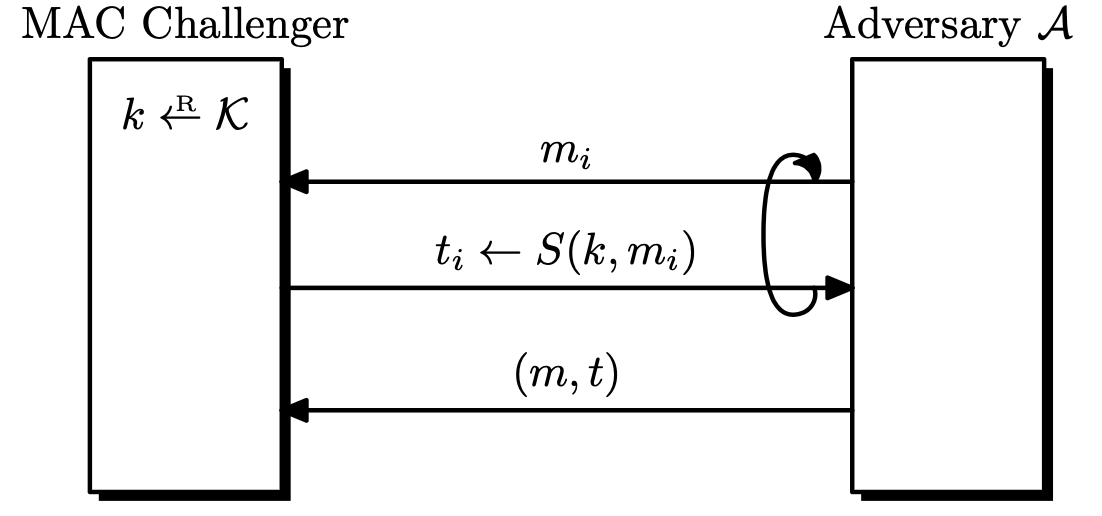
\includegraphics[width=0.5\linewidth]{figures/chapter6/fig2.png}
  \input{figures/chapter6/fig2.tex}
  \caption{MAC 攻击游戏(攻击游戏 \ref{game:6-1})}
  \label{fig:6-2}
\end{figure}

\begin{definition}\label{def:6-2}
如果对于所有有效对手 $\mathcal{A}$,${\rm MAC}\mathsf{adv}[\mathcal{A},\mathcal{I}]$ 的值都可忽略不计,我们就称 MAC 系统 $\mathcal{I}$ 是安全的。
\end{definition}

在对手赢得攻击游戏 \ref{game:6-1} 的情况下,它发送给挑战者的数对 $(m,t)$ 被称为\textbf{存在性伪造 (existential forgery)}。如果一个 MAC 系统满足定义 \ref{def:6-2},我们就称其在选择消息攻击下是\textbf{存在性不可伪造 (existential unforgeable)} 的。

在确定性 MAC 系统的情况下,$\mathcal{A}$ 赢得攻击游戏 \ref{game:6-1} 的唯一方法是为某个新消息 $m\notin\{m_1,m_2,\dots\}$  产生一个有效的消息-标签对 $(m,t)$。事实上,这种情况下的安全性只是意味着 $S$ 是\emph{不可预测的},参见 \ref{subsec:4-1-1} 小节给出的定义;也就是说,给定 $S(k,m_1),S(k,m_2),\dots$,对于任何 $m\notin\{m_1,m_2,\dots\}$,预测出 $S(k,m)$ 都是很难的。

在概率性 MAC 系统的情况下,我们的安全定义抓住了一个更强的属性。对于一条给定的消息,可能有许多条有效的标签。假设 $m$ 是某一条消息,又假设对手请求了 $m$ 的一条或多条有效标签 $t_1,t_2,\dots$,那么对手能否为 $m$ 产生一条新的有效标签 $t'$?(即一个满足 $t'\notin\{t_1,t_2,\dots\}$ 的标签)。我们的定义表明,对于一个有效对 $(m,t')$,如果 $t'$ 是新的,它就是一个有效的存在性伪造。因此,为了使 MAC 是安全的,对手必须很难为先前已经签署的消息 $m$ 产生一个新的有效标签 $t'$,这个对 MAC 的要求似乎很奇怪。如果对手已经有了 $m$ 的有效标签,我们为什么还要关心它是否能产生另一个呢?正如我们将要在第\ref{chap:9}章看到的,我们的安全定义,即防止对手在已签名的消息上产生新的标签,对于我们所考虑的应用是必要的。

回顾一下引言中的两个例子,我们可以发现,存在性不可伪造性意味着攻击者不能用一个有效标签来创建一条假的新闻报道。同样地,攻击者不能在篡改磁盘上程序的同时还不使程序的标签无效。但是,请注意,当使用 MAC 来保护应用程序的代码时,用户必须在每次要运行应用程序时提供他们的 MAC 密钥,这是一个很烦人的事情。在第\ref{chap:8}章,我们会讨论一种可以保护公共应用程序代码的无密钥方法。

为了深化对安全 MAC 的理解,我们不妨看几个案例。令 $\mathcal{I}=(S,V)$ 是一个定义在 $(\mathcal{K},\mathcal{M},\mathcal{T})$ 上的 MAC,令 $k$ 是 $\mathcal{K}$ 上的一个随机密钥。

\begin{example}\label{exmp:6-3}
假设 $m_1$ 和 $m_2$ 是几乎相同的两条消息。比如,$m_1$ 是一张 $100$ 美元的汇款单,而 $m_2$ 是一张 $101$ 美元的汇款单。显然,一个截获了 $m_1$ 的有效标签的对手不应当能够从中推导出$m_2$ 的有效标签。一个满足定义 \ref{def:6-2} 的 MAC 系统可以确保这一点。为了了解原因,假设一个对手 $\mathcal{A}$ 能够在给定 $m_1$ 的标签的情况下伪造 $m_2$ 的标签。那么,$\mathcal{A}$ 就可以赢得攻击游戏 \ref{game:6-1},方法是使用选择消息攻击来请求 $m_1$ 的标签,然后据此推导出 $m_2$ 的伪造标签 $t_2$,并输出 $(m_2,t_2)$ 作为有效的存在性伪造。显然,$\mathcal{A}$ 赢得了攻击游戏 \ref{game:6-1}。因此,存在性不可伪造性抓住了这样一个事实,即消息 $m_1$ 的标签对于产生另一条消息 $m_2$ 的标签来说不会提供任何有用的信息,即使 $m_2$ 和 $m_1$ 是几乎相同的。
\end{example}

\begin{example}\label{exmp:6-4}
我们对安全的 MAC 的定义使对手有能力获得任意消息的标签,这似乎是给了对手太多的权力。然而,在实践中,许多情况下,选择消息攻击是可行的。原因是 MAC 签名者往往不知道被签名数据的来源。例如,考虑一个将磁盘内容转储到备份磁带上的备份系统。由于备份的完整性是很重要的,系统为每一个将要被写入磁带的磁盘分组计算出一个完整性标签。该标签与数据分组一起被存储到磁带上。现在,假设一个攻击者将数据写到磁盘的低安全性区域。攻击者的数据将被备份,系统将对其计算出一个标签。通过检查所生成的备份磁带,攻击者就能获得它所选择的消息的标签。如果 MAC 系统对选择消息攻击是安全的,那么这种操作并不能帮助攻击者破解系统。
\end{example}

\begin{remark}\label{remark:6-1}
就像我们对其他安全原语所做的那样,我们可以把安全的 MAC 的概念推广到多密钥设置中,并证明一个安全的 MAC 在多密钥设置中也是安全的。参见练习 \ref{exer:6-3}。
\end{remark}

\subsection{数学细节}\label{subsec:6-1-1}

和之前一样,我们使用 \ref{sec:2-3} 节中定义的术语,对 MAC 给出一个更精确的数学定义。读者在初读时可以安全地跳过这一小节。

\begin{definition}[MAC]\label{def:6-3}
一个 \textbf{MAC} 系统是一对有效算法 $S$ 和 $V$,以及三个具有系统参数化 $P$ 的空间族:
\[
\mathbf{K}=\{\mathcal{K}_{\lambda,\Lambda}\}_{\lambda,\Lambda},\quad
\mathbf{M}=\{\mathcal{M}_{\lambda,\Lambda}\}_{\lambda,\Lambda},\quad
\mathbf{T}=\{\mathcal{T}_{\lambda,\Lambda}\}_{\lambda,\Lambda}
\]
和之前一样,$\lambda\in Z_{\geq1}$ 是一个安全参数,$\Lambda\in{\rm Supp}(P(\lambda))$ 是一个领域参数。我们要求:
\begin{enumerate}
	\item $\mathbf{K}$,$\mathbf{M}$ 和 $\mathbf{T}$ 是可有效识别的。
	\item $\mathbf{K}$ 是可有效采样的。
	\item 算法 $S$ 是一个有效的概率性算法,对于输入 $\lambda\in\mathbb{Z}_{\geq1}$,$\Lambda\in{\rm Supp}(P(\lambda))$,$k\in\mathcal{K}_{\lambda,\Lambda}$ 和 $m\in\mathcal{M}_{\lambda,\Lambda}$,$S$ 输出 $\mathcal{T}_{\lambda,\Lambda}$ 中的一个元素。
	\item 算法 $V$ 是一个有效确定性算法,对于输入 $\lambda\in\mathbb{Z}_{\geq1}$,$\Lambda\in{\rm Supp}(P(\lambda))$,$k\in\mathcal{K}_{\lambda,\Lambda}$,$m\in\mathcal{M}_{\lambda,\Lambda}$ 和 $t\in\mathcal{T}_{\lambda,\Lambda}$,$V$ 输出 $\mathsf{accept}$ 或 $\mathsf{reject}$。
\end{enumerate}

\end{definition}

在定义安全性时,我们通过安全参数 $\lambda$ 将攻击游戏 \ref{game:6-1} 参数化,对手和挑战者都会得到该参数。因此,优势 ${\rm MAC}\mathsf{adv}[\mathcal{A},\mathcal{I}]$ 也是 $\lambda$ 的一个函数。定义 \ref{def:6-2} 应该被理解为 ${\rm MAC}\mathsf{adv}[\mathcal{A},\mathcal{I}](\lambda)$ 是一个可忽略不计函数。
\section{MAC验证查询不会帮助攻击者}\label{sec:6-2}

在我们对安全的 MAC 的定义(攻击游戏 \ref{game:6-1})中,对手没有办法测试一个给定的信息-标签对是否有效。事实上,对手甚至无法判断它是否赢得了游戏,因为只有挑战者拥有运行验证算法所需的密钥。在现实生活中,一个有能力发动选择消息攻击的攻击者可能也能测试一个给定的消息-标签对是否有效。例如,攻击者可以建立一个有问题的消息-标签对数据包,并将它发送到受害者的机器上。然后,通过查看机器的行为,攻击者就可以知道该数据包是被接受了还是被丢弃了,进而确定该标签是否有效。

因此,通过赋予对手验证信息-标签对的额外权力来扩展攻击游戏 \ref{game:6-1} 是合理的。当然,我们仍然允许对手为它选择的任意消息请求标签。

\begin{game}[允许验证查询的 MAC 安全性]\label{game:6-2}
对于定义在 $(\mathcal{K},\mathcal{M},\mathcal{T})$ 上的一个给定的 MAC 系统 $\mathcal{I}=(S,V)$,以及一个给定的对手 $\mathcal{A}$,攻击游戏运行如下:
\begin{itemize}
	\item 挑战者随机选取 $k\overset{\rm R}\leftarrow\mathcal{K}$。
	\item $\mathcal{A}$ 向挑战者发起多次查询,每次查询可以是下面两种类型之一:
	\begin{itemize}
		\item \emph{签名查询}:对于 $i=1,2,\dots$,第 $i$ 次签名查询的内容是一条消息 $m_i\in\mathcal{M}$。挑战者计算出一个标签 $t_i\overset{\rm R}\leftarrow S(k,m_i)$,然后将 $t_i$ 交给 $\mathcal{A}$。
		\item \emph{验证查询}:对于 $j=1,2,\dots$,第 $j$ 次验证查询的内容是一个消息-标签对 $(\hat m_j,\hat t_j)\in\mathcal{M}\times\mathcal{T}$,该数对不在之前的签名对中,即:
		\[(\hat m_j,\hat t_j)\notin\{(m_1,t_1),(m_2,t_2),\dots\}\]
		挑战者将 $V(k,\hat m_j,\hat t_j)$ 发送给 $\mathcal{A}$。
	\end{itemize}
\end{itemize}
如果挑战者针对上述所有验证查询中的至少一个给出了 $\mathsf{accept}$ 的应答,我们就称 $\mathcal{A}$ 赢得了上述游戏。我们将 $\mathcal{A}$ 就 $\mathcal{I}$ 的优势表示为 ${\rm MAC^{vq}}\mathsf{adv}[\mathcal{A},\mathcal{I}]$,即 $\mathcal{A}$ 赢得该游戏的概率。
\end{game}

\begin{snote}[两个定义是等价的。]
攻击游戏 \ref{game:6-2} 在本质上与之前的攻击游戏 \ref{game:6-1} 是相同的,只是 $\mathcal{A}$ 可以发出 MAC 验证查询。我们证明,这种额外的权力并不能够帮助对手。
\end{snote}

\begin{theorem}\label{theo:6-1}
如果 $\mathcal{I}$ 是一个安全的 MAC 系统,那么它在存在验证查询的情况下也是安全的。
\begin{quote}
特别地,对于每个按照攻击游戏 \ref{game:6-2} 攻击 $\mathcal{I}$ 的 MAC 对手 $\mathcal{A}$,如果它最多能够发起 $Q_{\rm v}$ 次验证查询和 $Q_{\rm s}$ 次签名查询,则存在一个按照攻击游戏 \ref{game:6-1} 攻击 $\mathcal{I}$ 的 $Q_{\rm s}$ 次查询 MAC 对手 $\mathcal{B}$,其中 $\mathcal{B}$ 是一个围绕 $\mathcal{A}$ 的基本包装器,使得:
\end{quote}
\[
{\rm MAC^{vq}}\mathsf{adv}[\mathcal{A},\mathcal{I}]\leq{\rm MAC}\mathsf{adv}[\mathcal{A},\mathcal{I}]\cdot Q_{\rm v}
\]
\end{theorem}

\begin{proof}[证明思路]
假设 $\mathcal{A}$ 是一个 MAC 对手,它像攻击游戏 \ref{game:6-2} 中那样攻击 $\mathcal{I}$,并且最多进行 $Q_{\rm v}$ 次验证查询和 $Q_{\rm s}$ 次签名查询。我们可以基于对手 $\mathcal{A}$ 建立一个对手 $\mathcal{B}$,它如攻击游戏 \ref{game:6-1} 中那样攻击 $\mathcal{I}$,并最多进行 $Q_{\rm s}$ 次签名查询。对手 $\mathcal{B}$ 可以很容易地应答 $\mathcal{A}$ 的签名查询,只需要将这些查询转发给 $\mathcal{B}$ 的挑战者,并将挑战者产生的标签转发给 $\mathcal{A}$ 即可。

问题在于如何应答 $\mathcal{A}$ 的验证查询。根据定义,$\mathcal{A}$ 只会对不在之前已经签署的消息对中的消息提交验证查询。因此,$\mathcal{B}$ 可以采取一个简单的策略,即对 $\mathcal{A}$ 的所有验证查询都回复 $\mathsf{reject}$。如果 $\mathcal{B}$ 的回答是错的,它就得到了一个能够让它赢得攻击游戏 \ref{game:6-1} 的伪造消息。不幸的是,$\mathcal{B}$ 并不知道这些验证查询中的哪一个是伪造的,所以它只能猜测,也就是随机选择一个。由于 $\mathcal{A}$ 最多能发出 $Q_{\rm v}$ 次验证查询,所以 $\mathcal{B}$ 将以至少 ${1}/{Q_{\rm v}}$ 的概率猜对。这就是误差项中 $Q_{\rm v}$ 因子的来源。
\end{proof}

\begin{proof}
更详细地说,对手 $\mathcal{B}$ 在攻击游戏 \ref{game:6-2} 中扮演 $\mathcal{A}$ 的挑战者,同时在攻击游戏 \ref{game:6-1} 中扮演对手,并与该游戏中的 MAC 挑战者交互。它的工作逻辑如下:

\vspace{5pt}

\hspace*{5pt} 初始化:\\
\hspace*{50pt} 选取 $\omega\overset{\rm R}\leftarrow\{1,\dots,Q_{\rm v}\}$\\
\hspace*{26pt} 当从 $\mathcal{A}$ 处收到签名查询 $m_i\in\mathcal{M}$ 时:\\
\hspace*{50pt} 将 $m_i$ 转发给 MAC 挑战者,并获得标签 $t_i$\\
\hspace*{50pt} 将 $t_i$ 发送给 $\mathcal{A}$\\
\hspace*{26pt} 当从 $\mathcal{A}$ 处收到的验证查询 $(\hat m_j,\hat t_j)\in\mathcal{M}\times\mathcal{T}$ 时:\\
\hspace*{50pt} 如果 $j=\omega$:\\
\hspace*{75pt} 输出 $(\hat m_j,\hat t_j)$ 作为一个候选的伪造对,然后停机\\
\hspace*{50pt} 否则:\\
\hspace*{75pt} 向 $\mathcal{A}$ 发送 $\mathsf{reject}$

\vspace{5pt}

为了严格论证对手 $\mathcal{B}$ 的构造,我们分析 $\mathcal{A}$ 在以下三个密切相关的游戏中的行为。

\vspace{5pt}

\noindent\textbf{游戏$\mathbf{0}$}。
这是原始的攻击游戏,就如攻击游戏 \ref{game:6-2} 中 $\mathcal{A}$ 与挑战者之间进行的游戏一样。挑战者在该游戏中的逻辑如下:

\vspace{5pt}

\hspace*{5pt} 初始化:\\
\hspace*{50pt} 选取 $k\overset{\rm R}\leftarrow\mathcal{K}$\\
\hspace*{26pt} 当从 $\mathcal{A}$ 处收到签名查询 $m_i\in\mathcal{M}$ 时:\\
\hspace*{50pt} 令 $t_i\overset{\rm R}\leftarrow S(k,m_i)$\\
\hspace*{50pt} 将 $t_i$ 发送给 $\mathcal{A}$\\
\hspace*{26pt} 当从 $\mathcal{A}$ 处收到的验证查询 $(\hat m_j,\hat t_j)\in\mathcal{M}\times\mathcal{T}$ 时:\\
\hspace*{50pt} 令 $r_j\leftarrow V(k,\hat m_j,\hat t_j)$\\
\hspace*{10pt} ($*$)
\hspace*{19.5pt} 将 $r_j$ 发送给 $\mathcal{A}$

\vspace{5pt}


记 $W_0$ 为在游戏 $0$ 中,存在某个 $j$ 使得 $r_j=\mathsf{accept}$ 的事件。显然:
\begin{equation}\label{eq:6-1}
\Pr[W_0]={\rm MAC^{vq}}\mathsf{adv}[\mathcal{A},\mathcal{I}]
\end{equation}

\noindent\textbf{游戏$\mathbf{1}$}。
游戏 $1$ 与游戏 $0$ 基本相同,只是将游戏 $0$ 中标有 ($*$) 的一行改为:

\vspace{5pt}

\hspace*{50pt} 将 $\mathsf{reject}$ 发送给 $\mathcal{A}$

\vspace{5pt}

也就是说,在游戏 $1$ 中,在应答验证查询时,挑战者总是用 $\mathsf{reject}$ 来回应 $\mathcal{A}$。我们定义 $W_1$ 为在游戏 $1$ 中,存在某个 $j$ 使得 $r_j=\mathsf{accept}$ 的事件。尽管在游戏 $1$ 中,挑战者不会通知 $\mathcal{A}$ 事件 $W_1$ 发生了,但是在这个事件发生之前,游戏 $0$ 和游戏 $1$ 的进程事实上都是完全相同的,因此事件 $W_0$ 和 $W_1$ 在本质上是相同的,因此:
\begin{equation}\label{eq:6-2}
\Pr[W_1]=\Pr[W_0]
\end{equation}
此外,注意到,在游戏 $1$ 中,尽管 $r_j$ 被用来定义获胜的条件,但它们并没有被用于任何其他目的,因此不会以任何方式影响攻击。

\vspace{5pt}

\noindent\textbf{游戏$\mathbf{2}$}。
游戏 $2$ 与游戏 $1$ 基本相同,只是在游戏开始时,挑战者随机选取 $\omega\overset{\rm R}\leftarrow\{1,\dots,Q_{\rm v}\}$。我们定义 $W_2$ 为游戏 $2$ 中 $r_\omega=\mathsf{accept}$ 成立的事件。由于 $\omega$ 的选择与攻击本身无关,我们有:
\begin{equation}\label{eq:6-3}
\Pr[W_2]\geq{\Pr[W_1]}/{Q_{\rm v}}
\end{equation}

显然,根据构造,我们有:
\begin{equation}\label{eq:6-4}
\Pr[W_2]={\rm MAC}\mathsf{adv}[\mathcal{B},\mathcal{I}]
\end{equation}
于是,根据式 \ref{eq:6-1},\ref{eq:6-2} 和 \ref{eq:6-3},我们就能得到该定理成立。
\end{proof}

综上所述,我们表明,给予对手更多权力的攻击游戏 \ref{game:6-2} 和定义安全的 MAC 时使用的攻击游戏 \ref{game:6-1} 是等价的。这种归约在误差项中引入了一个 $Q_{\rm v}$ 的系数。在本书中,我们将使用这两个攻击游戏:
\begin{itemize}
	\item 当构建安全的 MAC 时,使用攻击游戏 \ref{game:6-1} 更容易,它限制对手只能发起签名查询。这使得我们更容易证明安全性,因为我们只需要考虑一种类型的查询。我们将在整个章节中使用这个攻击游戏。
	\item 当使用安全的 MAC 来构建更高层次的系统(如验证式加密)时,假设 MAC 对于攻击游戏 \ref{game:6-2} 中描述的更强的对手是安全的,是更方便的。
\end{itemize}

我们还指出,如果我们使用一个较弱的安全概念,即对手只通过在新消息上给出一个有效标签(而不是新的有效的消息-标签对)而获胜,那么攻击游戏 \ref{game:6-1} 和攻击游戏 \ref{game:6-2} 的类比就\emph{不}等价了(见练习 6.7)。
\section{使用 PRF 构建 MAC}\label{sec:6-3}

我们下面尝试使用我们已经掌握的工具来构建安全的 MAC。在前几章中,我们使用伪随机函数 (PRF) 来构建各种加密系统。我们举了一些实际的 PRF 的例子,比如 AES(虽然 AES 是一个分组密码,但由于 PRF 切换引理,即定理 \ref{theo:4-4},我们也可将其看作是一个 PRF)。在这里,我们表明,任何安全的 PRF 都可以直接被用来建立一个安全的 MAC。

回顾一下,PRF 是这样的一种算法 $F$,它接受密钥 $k$ 和数据分组 $x$ 作为输入,并输出一个值 $y:=F(k,x)$。通常,如果密钥在 $\mathcal{K}$ 上,输入在 $\mathcal{X}$ 上,输出在 $\mathcal{Y}$ 上,我们就称 $F$ 定义在 $(\mathcal{K},\mathcal{X},\mathcal{Y})$ 上。对于一个 PRF $F$,我们将\textbf{由 $F$ 派生出的确定性 MAC 系统} $\mathcal{I}=(S,V)$ 定义为:

\vspace{5pt}

\hspace*{5pt} $S(k,m)=F(k,m)$;

\vspace{5pt}

\hspace*{5pt} $
V(k,m,t)=\left\{
\begin{array}{ll}
\mathsf{accept}, & F(k,m)=t\\
\mathsf{reject}, & \text{otherwise}
\end{array}
\right.
$

\vspace{8pt}

正如已经讨论过的,任何具有大的(即超多项式的)输出空间的 PRF 都是不可预测的(见 \ref{subsec:4-1-1} 小节),因此,正如 \ref{sec:6-1} 节所讨论的,上述构造产生了一个安全的 MAC。完整起见,我们下面用一个定理来说明这一点。

\begin{theorem}\label{theo:6-2}
令 $F$ 是一个定义在 $(\mathcal{K},\mathcal{X},\mathcal{Y})$ 上的安全的 PRF,其中 $|\mathcal{Y}|$ 是超多项式的。那么,由 $F$ 派生的确定性 MAC 系统 $\mathcal{I}$ 是一个安全的 MAC。
\begin{quote}
特别地,对于每个按照攻击游戏 \ref{game:6-1} 攻击 $\mathcal{I}$ 的 $Q$ 次查询 MAC 对手 $\mathcal{A}$,都存在一个按照攻击游戏 \ref{game:4-2} 攻击 $F$ 的 $(Q+1)$ 次查询 PRF 对手 $\mathcal{B}$,其中 $\mathcal{B}$ 是一个围绕 $\mathcal{A}$ 的基本包装器,满足:
\end{quote}
\[
{\rm MAC}\mathsf{adv}[\mathcal{A},\mathcal{I}]\leq{\rm PRF\mathsf{adv}}[\mathcal{B}, F]+{1}/{|\mathcal{Y}|}
\]
\end{theorem}

\begin{proof}[证明思路]
令 $\mathcal{A}$ 是一个有效 MAC 对手。我们通过约束 $\mathcal{A}$ 产生伪造的信息-标签对的能力,推导出 ${\rm MAC}\mathsf{adv}[\mathcal{A},\mathcal{I}]$ 的上界。和之前一样,用 ${\rm Funs}[\mathcal{X},\mathcal{Y}]$ 中的一个真随机函数 $f$ 替换底层的安全 PRF $F$ 并不会使 $\mathcal{A}$ 的优势发生很大的变化。但是,如果对手 $\mathcal{A}$ 交互的对象是一个真随机函数,它将会面临一个没有希望的任务:它需要在它选定的几个点上获取 $f$ 的值,并发动选择消息攻击。然后,它需要猜测 $f(m)\in\mathcal{Y}$ 在某个新的点 $m$ 处的值。但由于 $f$ 是一个真随机函数,$\mathcal{A}$ 没有办法获得任何关于 $f(m)$ 的信息,因此它猜中 $f(m)$ 的概率微乎其微。
\end{proof}

\begin{proof}
我们通过让 $\mathcal{A}$ 与两个密切相关的挑战者交互来证明这个结论。

\vspace{5pt}

\noindent\textbf{游戏$\mathbf{0}$}。
和之前一样,我们先回顾 MAC 攻击游戏 \ref{game:6-1} 中的挑战者,它此时被应用于 $\mathcal{I}$。在这个游戏中,挑战者的逻辑如下:

\vspace{5pt}

\hspace*{-16.5pt} ($*$)
\hspace*{1pt} 选取 $k\overset{\rm R}\leftarrow\mathcal{K}$,令 $f\leftarrow F(k,\cdot)$\\
\hspace*{26pt} 当收到第 $i$ 个签名查询 $m_i\in\mathcal{M}$ ($i=1,2,\dots$) 时:\\
\hspace*{50pt} 令 $t_i\leftarrow f(m_i)$\\
\hspace*{50pt} 将 $t_i$ 发送给对手

\vspace{5pt}

\noindent
在游戏结束时,对手输出一个消息-标签对 $(m,t)$。我们将 $W_0$ 定义为条件:
\begin{equation}\label{eq:6-5}
t=f(m)
\quad\quad\text{and}\quad\quad
m\notin\{m_1,m_2,\dots\}
\end{equation}
在游戏 $0$ 中成立的事件。显然,$\Pr[W_0]={\rm MAC}\mathsf{adv}[\mathcal{A},\mathcal{I}]$ 成立。

\vspace{5pt}

\noindent\textbf{游戏$\mathbf{1}$}。
接下来,和之前一样,我们打出``PRF牌",用 ${\rm Funs}[\mathcal{X},\mathcal{Y}]$ 中的一个真随机函数 $f$ 替换 $F(k,\cdot)$。直观地说,由于 $F$ 是一个安全的 PRF,对手 $\mathcal{A}$ 应该不会注意到这种差别。游戏 $1$ 中的挑战者与游戏 $0$ 中的挑战者大致相同,只是我们将标有 ($*$) 的那一行改为:

\vspace{5pt}

\hspace*{-16.5pt} ($*$)
\hspace*{1pt} 选取 $f\overset{\rm R}\leftarrow{\rm Funs}[\mathcal{X},\mathcal{Y}]$

\vspace{5pt}

\noindent
令 $W_1$ 为式 \ref{eq:6-5} 在游戏 $1$ 中成立的事件。我们构建一个 $(Q+1)$ 次查询 PRF 对手 $\mathcal{B}$,满足:
\begin{equation}\label{eq:6-6}
|\Pr[W_1]-\Pr[W_0]|={\rm PRF}\mathsf{adv}[\mathcal{B},F]
\end{equation}
对手 $\mathcal{B}$ 通过查询自己的 PRF 挑战者来应答 $\mathcal{A}$ 的选择消息查询。最终,$\mathcal{A}$ 会输出一个候选的 MAC 伪造 $(m,t)$,其中 $m$ 不在 $\mathcal{A}$ 之前的选择信息查询中。现在,$\mathcal{B}$ 在 $m$ 处向它的 PRF 挑战者发起查询,并得到某个 $t'\in\mathcal{Y}$。如果 $t=t'$,$\mathcal{B}$ 就输出 $0$,否则就输出 $1$。不难证明,这样的对手 $\mathcal{B}$ 满足式 \ref{eq:6-6}。

接下来我们直接约束 $\Pr[W_1]$。对手 $\mathcal{A}$ 得到了 $f$ 在 $m_1,m_2,\dots$ 处的值,然后被要求猜测 $f$ 在一个新点 $m$ 处的值。但由于 $f$ 是一个真随机函数,所以值 $f(m)$ 与它在其他点处的值都无关。由于 $m\notin\{m_1,m_2,\dots\}$,所以对手 $\mathcal{A}$ 将以 ${1}/{|\mathcal{Y}|}$ 的概率猜中 $f(m)$。因此,$\Pr[W_1]\leq{1}/{|\mathcal{Y}|}$。将此与式 \ref{eq:6-6} 结合,我们可以得到:
\[
{\rm MAC}\mathsf{adv}[\mathcal{A},\mathcal{I}]
=\Pr[W_0]
\leq\big\lvert\Pr[W_0]−\Pr[W_1]\big\rvert+\Pr[W_1]
\leq{\rm PRF}\mathsf{adv}[\mathcal{B},F]+\frac{1}{|\mathcal{Y}|}
\]
因此本定理得证。
\end{proof}

\begin{snote}[具体的标签长度。]
该定理表明,为确保 ${\rm MAC}\mathsf{adv}[\mathcal{A},\mathcal{I}]<2^{128}$,我们需要这样的一个 PRF,其输出空间 $\mathcal{Y}$ 满足 $|\mathcal{Y}|>2^{128}$。如果输出空间 $\mathcal{Y}$ 形如 $\{0,1\}^n$,其中 $n$ 是某个整数,那么产生的标签至少长 $128$ 比特。
\end{snote}
\section{用于长消息的无前缀PRF}\label{sec:6-4}

在上一节中,我们看到,任何一个安全的 PRF 也是一个安全的 MAC。然而,第\ref{chap:4}章中的 PRF 实例只接受短的输入,因而只能为非常短的消息提供完整性。比如,如果将 AES 看作是一个 PRF,我们就能得到一个用于 $128$ 比特消息的 MAC。现在,我们想要为更长的消息构建 MAC。

本章中所有的 MAC 构造都遵循同样的范式:它们从短输入的 PRF 开始(如 AES),产生一个 PRF,继而构造一个能用于更长输入的 MAC。因此,我们在本章的剩余部分的目标如下:
\begin{quote}
\textbf{给定一个针对短消息输入的安全 PRF,构建一个针对长消息输入的安全 PRF。}
\end{quote}
我们将会分三步来解决这个问题:
\begin{itemize}
	\item 首先,在本节中,我们为长输入构建\emph{无前缀安全的 PRF}。更确切地说,给定一个在单分组(比如 $128$ 比特)上运行的安全 PRF,我们想要构建一个无前缀的安全 PRF。回顾一下,无前缀安全 PRF(定义 \ref{def:4-5})只在有限的意义上是安全的:我们只要求\emph{无前缀对手}无法区分 PRF 和随机函数。一个无前缀 PRF 对手发出的查询是非空的分组序列,且其中的任何一个查询都不是其他查询的真前缀。
	\item 其次,在接下来的几节中,我们将展示如何把用于长输入的无前缀安全 PRF 转换成用于长输入的完全安全 PRF。因此,在这几节结束时,我们将得到几个这样的安全 PRF,并由此构造出能够用于长消息的安全的 MAC。
	\item 第三,在 \ref{sec:6-8} 节中,我们将展示,如何将一个作用于由分组序列构成的消息的 PRF 转换为一个作用于比特序列的 PRF。
\end{itemize}

\begin{snote}[无前缀的 PRF。]
我们从两个经典的无前缀安全 PRF 构造开始。图 \ref{fig:6-3-a} 展示了 \textbf{CBC} 构造,图 \ref{fig:6-3-b} 展示了\textbf{级联}构造。我们表明,当底层函数 $F$ 是一个安全的 PRF 时,CBC 构造和级联构造都是无前缀安全的 PRF。
\end{snote}

\begin{figure}
  \centering
  \subfigure[CBC构造$F_\mathrm{CBC}(k,m)$]{
    \input{figures/chapter6/fig3-a.tex}
  	\label{fig:6-3-a}
  }
  
  \,
  
  \,
  
  \subfigure[级联构造$F^*(k,m)$]{
  	\input{figures/chapter6/fig3-b.tex}
  	\label{fig:6-3-b}
  }
  \caption{两种无前缀安全的 PRF}
\end{figure}

\subsection{CBC无前缀安全PRF}

令 $F$ 是一个 PRF,它将 $n$ 比特的输入映射为 $n$ 比特的输出。$F$ 定义在 $(\mathcal{K},\mathcal{X},\mathcal{X})$ 上,其中 $\mathcal{X}=\{0,1\}^n$。对于任意多项式边界的值 $\ell$,我们构造一个新的 PRF $F_\mathrm{CBC}$,它能够将 $\mathcal{X}^{\leq\ell}$ 上的消息映射为 $\mathcal{X}$ 上的输出。图 \ref{fig:6-3-a} 中描述的函数 $F_\mathrm{CBC}$ 的工作原理如下:

\vspace*{5pt}

\hspace*{5pt} 输入:$k\in\mathcal{K}$ 和 $m=(a_1,\dots,a_v)\in\mathcal{X}^{\leq\ell}$,其中 $v\in\{0,\dots,\ell\}$\\
\hspace*{26pt} 输出:$\mathcal{X}$ 中的一个标签

\vspace*{5pt}

\hspace*{5pt} 令 $t\leftarrow0^n$\\
\hspace*{26pt} 对于 $i=1,\dots,v$:\\
\hspace*{50pt} 计算 $t\leftarrow F(k,\;a_i\oplus t)$\\
\hspace*{26pt} 输出 $t$

\vspace*{5pt}

\noindent
$F_{\rm CBC}$ 与图 \ref{fig:5-4}	中介绍的 CBC 模式加密类似,但是有两个重要的区别。首先,$F_\mathrm{CBC}$ 在 CBC 链中不会输出任何中间值。其次,$F_\mathrm{CBC}$ 使用一个固定的 IV,即 $0^n$,而 CBC 加密对每条消息中都使用一个随机的 IV。

下面的定理表明,$F_\mathrm{CBC}$ 是一种定义在 $(\mathcal{K},\mathcal{X}^{\leq l},\mathcal{X})$ 上的无前缀安全 PRF。

\begin{theorem}\label{theo:6-3}
令 $F$ 是一个定义在 $(\mathcal{K},\mathcal{X},\mathcal{X})$ 上的安全 PRF,其中 $\mathcal{X}=\{0,1\}^n$,$|\mathcal{X}|=2^n$ 是超多项式的。那么,对于任意多项式边界的值 $\ell$,$F_\mathrm{CBC}$ 都是一个定义在 $(\mathcal{K},\mathcal{X}^{\leq\ell},\mathcal{X})$ 上的无前缀安全 PRF。
\begin{quote}
特别地,对于任意如攻击游戏 \ref{game:4-2} 中那样攻击 $F_{\rm CBC}$ 的无前缀 PRF 对手 $\mathcal{A}$,如果它最多能够向其挑战者发起 $Q$ 次查询,则必然存在一个像攻击游戏 \ref{game:4-2} 中那样攻击 $F$ 的 PRF 对手 $\mathcal{B}$,其中 $\mathcal{B}$ 是一个围绕 $\mathcal{A}$ 的基本包装器,满足:
\end{quote}
\begin{equation}\label{eq:6-7}
{\rm PRF^{pf}\mathsf{adv}}[\mathcal{A},F_{\rm CBC}]\leq{\rm PRF\mathsf{adv}}[\mathcal{B},F]+\frac{(Q\ell)^2}{2|\mathcal{X}|}
\end{equation}
\end{theorem}

\noindent
练习 6.6 提出了一种针对定长 $F_\mathrm{CBC}$ 的攻击,并证明其安全性随 $Q$ 的增长而呈二次递减,这表明式 \ref{eq:6-7} 中的 $Q^2$ 项是必要的。一个更困难的安全性证明表明,安全性只随 $\ell$ 的增长线性递减(见第 \ref{sec:6-13} 节)。特别地,式 \ref{eq:6-7} 中的误差项可以被简化为一个以 $O(Q^2\ell/|\mathcal{X}|)$ 为主成分的表达式。

\begin{proof}[证明思路]
我们用一棵有根的树来表示对手的查询,树中的边以消息分组(即 $\mathcal{X}$ 中的元素)为标签。记 $m=(a_1,\dots,a_v)\in\mathcal{X}^{v}$,其中 $1\leq v\leq\ell$,则对 $F(k,m)$ 的一次查询就定义了一条树中的路径,该路径从根开始,如下所示:
\begin{equation}\label{eq:6-8}
root\overset{a_1}\longrightarrow p_1\overset{a_2}\longrightarrow p2 \overset{a_3}\longrightarrow\cdots \overset{a_v}\longrightarrow p_v
\end{equation}
因此,两条消息 $m$ 和 $m'$ 就对应着树中的两条从根开始的路径;这两条路径可能共享一个共同的初始子路径,该子路径就对应着 $m$ 和 $m'$ 的最长公共前缀。

对于这颗树上的每个节点 $p$,我们都将其与一个值 $\gamma_p\in\mathcal{X}$ 关联,该值代表 CBC 链中的计算结果。更确切地说,我们定义 $\gamma_{\rm root}:=0^n$,并且,对于任何非根节点 $q$ 及其父节点 $p$,如果树中的对应路径是 $p\overset{a}\rightarrow q$,那么 $\gamma_q:=F(k,\gamma_p\oplus a)$。有了这些约定,我们可以看到,如果一条消息 $m$ 所对应的路径如式 \ref{eq:6-8} 所示,则有 $\gamma_{p_v}=F_\mathrm{CBC}(k,m)$。

证明的关键是论证:如果 $F$ 表现得像一个随机函数,那么对于树中任意的一对不同的边,比如 $p\overset{a}\rightarrow q$ 和 $p'\overset{a'}\rightarrow q'$,$\gamma_p\oplus a\neq\gamma_{p'}\oplus a'$ 成立的概率都是压倒性的。为了证明不存在这种类型的碰撞,无前缀的限制至关重要,因为它能够保证对手永远不会看到 $\gamma_p$ 和 $\gamma_{p'}$,因此 $a$ 和 $a'$ 与这些值无关。一旦我们确定了不存在这种类型的碰撞,就会发现所有和非根节点相关的值都是随机和独立的,这一点尤其适用于与叶子结点相关的值,它们代表对手所看到的 $F_{\rm CBC}$ 的输出。因此,对手无法将 $F_{\rm CBC}$ 和真随机函数区分开来。
\end{proof}

\begin{proof}
为了让上面的叙述更加严谨,我们让 $\mathcal{A}$ 在四个游戏中与四个密切相关的挑战者进行交互。对于 $j=0,\dots,3$,我们令 $W_j$ 为 $\mathcal{A}$ 在游戏 $j$ 结束后输出 $1$ 的事件。

\vspace{5pt}

\textbf{游戏 $\mathbf{0}$}。
游戏 $0$ 就是攻击游戏 \ref{game:4-2} 的实验 $0$。

\vspace{5pt}

\textbf{游戏 $\mathbf{1}$}。
接下来,和之前一样,我们打出 ``PRF牌",用一个 ${\rm Funs}[\mathcal{X},\mathcal{X}]$ 中的真随机函数 $f$ 代替 $F(k,\cdot)$。显然,对于一个有效对手 $\mathcal{B}$,我们有:
\begin{equation}\label{eq:6-9}
\big\lvert
\Pr[W_1]-\Pr[W_0]
\big\rvert
={\rm PRF}\mathsf{adv}[\mathcal{B},F]
\end{equation}

\textbf{游戏 $\mathbf{2}$}。
接下来,我们做一个纯粹的概念上的改变,用``忠实的侏儒" 来实现随机函数 $f$(如 \ref{subsec:4-4-2} 小节中那样)。然而,我们以一种特殊的方式来进行实现,即使用上面介绍的``查询树"。

为此,我们首先令 $B:=Q\ell$,它代表 $f$ 被计算的次数的上界。我们的挑战者首先准备一系列的随机数:
\[
\beta_i\overset{\rm R}\leftarrow\mathcal{X}\quad
(i=1,\dots,B)
\]
这些随机数将会是我们的挑战者在游戏中所使用的仅有的几个随机值。

随着对手的查询,我们的挑战者将动态地建立起它的查询树。最初,查询树只有一个树根。每当对手进行查询时,挑战者就会在现有的查询树中加入新的路径;在某些时候,这个路径可能会延伸到现有的查询树之外,那么挑战者就会向树中添加必要的节点和边,以使查询树能够容纳新的查询路径。

我们的挑战者还必须计算与每个节点相关的 $\gamma_p$ 值。在最开始时,它只有 $\gamma_{\rm root}=0^n$。当在树中添加一条新边 $p\overset{a}\rightarrow q$ 时,如果这是被添加的第 $i$ 条边(对于 $i=1,\dots,B$),我们的挑战者会进行以下操作:

\vspace{8pt}

\hspace*{5pt} 令 $\gamma_q\leftarrow\beta_i$\\
\hspace*{1pt} ($*$)
\hspace*{4.5pt} 如果存在另一条边 $p'\overset{a'}\rightarrow q'$ 使得 $\gamma_{p'}\oplus a'=\gamma_p\oplus a$,则令 $\gamma_q\leftarrow\gamma_{q'}$

\vspace{8pt}

\noindent
我们的想法是,在我们准备的序列 $\beta_1,\dots,\beta_B$ 使用下一个还未使用的值作为 $\gamma_q$ 的``默认"值。标有 ($*$) 的那行进行了必要的一致性检查,这确保了我们的侏儒确实是忠实的。

由于这种修改纯粹只是概念上的,我们有:
\begin{equation}\label{eq:6-10}
\Pr[W_2]=\Pr[W_1]
\end{equation}

\textbf{游戏 $\mathbf{3}$}。
接下来,我们通过删除游戏 $2$ 中标有 ($*$) 的那行,使得我们的侏儒变得健忘。

为了分析这一变化的影响,令 $Z$ 为\emph{在游戏 3 中},存在不同的两条边 $p\overset{a}\rightarrow q$ 和 $p'\overset{a'}\rightarrow q'$ 使得 $\gamma_{p'}\oplus a'=\gamma_p\oplus a$ 成立的事件。

现在,游戏 $2$ 和游戏 $3$ 中唯一随机选择的值就是对手的随机选择,即$Coins$,以及一系列的 $\beta_1,\dots,\beta_B$。注意到,对于任意固定的 $Coins,\beta_1,\dots,\beta_B$ 的随机选择,如果 $Z$ 没有发生,那么实际上游戏 $2$ 和游戏 $3$ 的进程就是完全相同的。因此,我们可以利用差分引理(定理 \ref{theo:4-7}),得到:
\begin{equation}\label{eq:6-11}
\big\lvert\Pr[W_3]-\Pr[W_2]\big\rvert\leq\Pr[Z]
\end{equation}

接下来,我们约束 $\Pr[Z]$。考察两条不同的边 $p\overset{a}\rightarrow q$ 和 $p'\overset{a'}\rightarrow q'$。我们想要约束 $\gamma_{p'}\oplus a'=\gamma_p\oplus a$ 成立的概率。该等式与:
\begin{equation}\label{eq:6-12}
\gamma_{p'}\oplus\gamma_p =a'\oplus a
\end{equation}
等价。有两种情况需要考虑:

\emph{情况1:}$p=p'$。由于两条边是不同的,我们必有 $a'\neq a$,因此式 \ref{eq:6-12} 成立的概率为 $0$。

\emph{情况2:}$p\neq p'$。对手查询是无前缀的,这一要求意味着在游戏 $3$ 中,对手永远不会看到或了解到关于 $\gamma_p$ 和 $\gamma_{p'}$ 的任何信息。$p$ 和 $p'$ 中的一个可能是根节点,但不可能两个都是。由此可见,$\gamma_{p'}\oplus\gamma_p$ 的值均匀分布在 $\mathcal{X}$ 上,且与 $a\oplus a'$ 无关。因此,式 \ref{eq:6-12} 成立的概率为 ${1}/{|\mathcal{X}|}$。

根据联合约束,可以得到:
\begin{equation}\label{eq:6-13}
\Pr[Z]\leq\frac{B^2}{2|\mathcal{X}|}
\end{equation}

将式 \ref{eq:6-9},\ref{eq:6-10},\ref{eq:6-11} 和\ref{eq:6-13} 相结合,我们得到:
\begin{equation}\label{eq:6-14}
{\rm PRF^{pf}}\mathsf{adv}[\mathcal{A},F_{\rm CBC}]=
\big\lvert\Pr[W_3]-\Pr[W_0]\big\rvert\leq{\rm PRF}\mathsf{adv}[\mathcal{B},F]+\frac{B^2}{2|\mathcal{X}|}
\end{equation}
此外,游戏 $3$ 完全对应于攻击游戏 \ref{game:4-2} 的实验 $1$,因此,该定理得证。
\end{proof}

\subsection{级联无前缀安全PRF}\label{subsec:6-4-2}

令 $F$ 是一个 PRF,它接受 $\mathcal{K}$ 中的密钥并输出 $\mathcal{K}$ 中的元素。我们称 $F$ 定义在 $(\mathcal{K},\mathcal{X},\mathcal{K})$ 上。对于任意多项式边界的值 $\ell$,我们建立一个新的 PRF $F^*$,称为 \textbf{$F$ 的级联 (cascade of $F$)},它将 $\mathcal{X}^{\leq\ell}$ 中的消息映射为 $\mathcal{K}$ 上的输出,如图 \ref{fig:6-3-b} 所示,该构造的原理如下:

\vspace*{5pt}

\hspace*{5pt} 输入:$k\in\mathcal{K}$ 和 $m=(a_1,\dots,a_v)\in\mathcal{X}^{\leq\ell}$,其中 $v\in\{0,\dots,\ell\}$\\
\hspace*{26pt} 输出:$\mathcal{K}$ 中的一个标签

\vspace*{5pt}

\hspace*{5pt} 令 $t\leftarrow k$\\
\hspace*{26pt} 对于 $i=1,\dots,v$:\\
\hspace*{50pt} 计算 $t\leftarrow F(t,\;a_i)$\\
\hspace*{26pt} 输出 $t$

\vspace*{5pt}

\noindent
下面的定理将表明,$F^*$ 是一个无前缀安全的 PRF。

\begin{theorem}\label{theo:6-4}
令 $F$ 是一个定义在 $(\mathcal{K},\mathcal{X},\mathcal{K})$ 上的安全的 PRF。那么,对于任意多项式边界的值 $\ell$,$F$ 的级联 $F^*$ 是一个定义在 $(\mathcal{K},\mathcal{X}^{\leq\ell},\mathcal{K})$ 上的无前缀安全的 PRF。
\begin{quote}
特别地,对于任意如攻击游戏 \ref{game:4-2} 中那样攻击 $F^*$ 的无前缀 PRF 对手 $\mathcal{A}$,假设它最多能够向其挑战者发起 $Q$ 次查询,则必然存在一个像攻击游戏 \ref{game:4-2} 中那样攻击 $F$ 的 PRF 对手 $\mathcal{B}$,其中 $\mathcal{B}$ 是一个围绕 $\mathcal{A}$ 的基本包装器,满足:
\end{quote}
\begin{equation}\label{eq:6-15}
{\rm PRF^{pf}\mathsf{adv}}[\mathcal{A},F^*]\leq Q\ell\cdot{\rm PRF\mathsf{adv}}[\mathcal{B},F]
\end{equation}
\end{theorem}

练习 6.6 提出了一种针对定长 $F^*$ 的攻击,并证明其安全性随 $Q$ 的增长而四次方递减。这令人不安,因为它似乎与式 \ref{eq:6-15} 中对 $Q$ 的线性依赖相矛盾。然而,请读者放心,这里其实并没有矛盾。练习 6.6 中的对手使用 $\ell=3$,当 $Q$ 大约为 $\sqrt{|\mathcal{K}|}$ 时,其优势约为 $1/2$。将 $\mathcal{A}$ 接入定理 \ref{theo:6-4} 的证明中,我们就能够得到一个 PRF 对手 $\mathcal{B}$,它在攻击 PRF $F$ 时大约进行 $Q$ 次查询,获得的优势大约是 $1/Q$。注意到,当 $Q$ 接近 $\sqrt{|\mathcal{K}|}$ 时,我们有 $1/Q\approx|\mathcal{K}|$ 这样的近似关系。这样的对手 $\mathcal{B}$ 并不令人惊讶:它本质上就是练习 4.27 中的通用 PRF 攻击者。因此,式 \ref{eq:6-15} 与练习 6.6 中的攻击本质上是一致的。另一种视角是,式 \ref{eq:6-15} 中已经出现了对 $Q$ 的二次依赖,因为有一个隐藏的 $Q$ 的因子被包含在了 ${\rm PRF\mathsf{adv}}[\mathcal{B},F]$ 这个量中。

\vspace{5pt}

证明定理 \ref{theo:6-4} 与证明 \ref{sec:4-6} 节中的变长树构造是一个无前缀安全的 PRF(定理 \ref{theo:4-11})是相似的。我们下面简单介绍一下如何扩展定理 \ref{theo:4-11} 的证明来证明定理 \ref{theo:6-4}。

\begin{snote}[与树构造的关系。]
级联构造是 \ref{sec:4-6} 节中介绍的变长树构造的一个推广。回顾一下,树构造使用一个安全的 PRG 建立一个安全的 PRF,该 PRG 将一个种子映射到一对种子。不难发现,当 $F$ 是定义在 $(\mathcal{K},\{0,1\},\mathcal{K})$ 上的 PRF 时,定理 \ref{theo:6-4} 就是定理 \ref{theo:4-11} 的直接推论:我们只要定义 PRG $G$ 为 $G(k):=(F(k,0),F(k,1))\in\mathcal{K}^2$,并且观察到用于 $F$ 的级联构造与用于 $G$ 的变长树构造本质上是相同的。

定理 \ref{theo:4-11} 的证明很容易推广到对任何 PRF 证明定理 \ref{theo:6-4}。比如说,假设 $F$ 定义在 $(\mathcal{K},\{0,1,2\},\mathcal{K})$ 上,那么它就对应于一个 PRF $G$,它将 $k\in\mathcal{K}$ 映射为 $G(k):=(F(k,0),F(k,1),F(k,2))\in\mathcal{K}^3$。如果我们将用于 $F$ 的级联构造看作是一颗三叉树而不是二叉树,那么甚至不需要修改太多,就可以套用定理 \ref{theo:4-11} 的证明。

但为什么要在宽度为 $3$ 的情况下停止呢?我们可以按我们的期望任意设定树的宽度。基于一个定义在 $(\mathcal{K},\mathcal{X},\mathcal{K})$ 上的PRF $F$ 的级联构造就对应于一棵宽度为 $|\mathcal{X}|$ 的树。同样地,定理 \ref{theo:4-11} 的证明也没有发生本质的变化。我们把细节留给感兴趣的读者作为练习(可以参考练习 4.26)。
\end{snote}

\begin{snote}[CBC 和级联 PRF 的对比。]
请注意,CBC 对 $F$ 的所有应用都使用同一个固定的密钥 $k$,而级联构造在每一轮中都使用不同的密钥。由于分组密码通常会使用相同的密钥来加密许多分组,因此级联构造中的密钥更新有可能导致比 CBC 更差的性能。因此,当使用像 AES 这样的现成的分组密码时,CBC 是更加自然的选择。

级联构造的一个优点是,式 \ref{eq:6-15} 中的上界中没有误差项。因此,即使底层 PRF 所依赖的领域 $\mathcal{X}$ 相对较小,级联构造仍然是安全的。相对地,CBC 只有在 $\mathcal{X}$ 大的时候才是安全的。因此,级联构造可以用来将 PRG 转换成大输入的 PRF,而 CBC 不能。
\end{snote}

\subsection{CBC 和级联 PRF 都是不安全的 MAC}

我们表明,从 CBC 和级联构造派生出来的 MAC 都是不安全的。这意味着 CBC 和级联构造都不是安全的 PRF。而我们在之前的章节中所展示的只是,CBC 和级联构造是\emph{无前缀}安全的 PRF。

\begin{snote}[对级联构造的扩展攻击。]
对于 $\mathcal{X}^{\leq\ell}$ 中的某条消息 $m$,给定 $F^*(k,m)$,对于任何的 $m'\in\mathcal{X}^*$,即使不知道 $k$,任何人也都能计算:
\begin{equation}\label{eq:6-16}
t':=F^*(k,\;m\,\Vert\,m')
\end{equation}
一旦 $F^*(k,m)$ 已知,任何人都可以用消息 $m'$ 的分组继续评估链,并最终得到 $t'$。我们把这称为级联构造的\textbf{扩展属性 (extension property)}。

扩展属性意味着,由 $F^*$ 派生而来的 MAC 是非常不安全的。伪造者可以首先请求消息 $m$ 的 MAC,然后对于任意的 $m'$,伪造者都可以推导出 $m\,\Vert\,m'$ 的 MAC。因此,根据定理 \ref{theo:6-2},$F^*$ 不是一个安全的 PRF。
\end{snote}

\begin{snote}[一种针对 CBC 的攻击。]
我们下面描述一种针对由 CBC 派生出的 MAC 的 MAC 伪造器。该伪造器的工作原理如下:
\begin{enumerate}
	\item 挑选一个任意的 $a_1\overset{\rm R}\leftarrow\mathcal{X}$;
	\item 请求单分组消息 $(a_1)$ 的标记 $t$;
	\item 定义 $a_2:=a_1\oplus t$,并输出 $t$ 作为两分组消息 $(a_1,a_2)\in\mathcal{X}$ 的 MAC 伪造。
\end{enumerate}
注意到 $t=F(k,a_1)$,$a_1=F(k,a_1)\oplus a_2$。根据 CBC 的定义,我们有:
\[
F_{\rm CBC}(k,(a_1,a_2))=F(k,F(k,a_1)\oplus a_2)=F(k,a_1)=t
\]
因此,$((a_1,a_2),t)$  是一个针对由 CBC 派生的 MAC 的存在性伪造。所以 $F_{\rm CBC}$ 无法成为一个安全的 PRF。请注意,对级联构造 MAC 的攻击远比对 CBC MAC 的攻击更具破坏性。但无论如何,这些攻击都表明,CBC 和级联构造都不应该被直接当作 MAC 使用。
\end{snote}
\section{从无前缀安全PRF到完全安全PRF(方法1):加密PRF}\label{sec:6-5}

我们下面展示如何将无前缀安全的 PRF $F_{\rm CBC}$ 和 $F^*$ 转换为安全的 PRF,这将为我们提供针对变长输入的安全 MAC。更一般地,我们将展示如何将无前缀安全的 PRF $PF$ 转换为完全安全的 PRF。我们会介绍以下三种方法:
\begin{itemize}
	\item 加密 PRF:用另一个 PRF 对 $PF$ 的短输出进行加密。
	\item 无前缀编码:对 $PF$ 的输入进行编码,使得任意一个输入都不是其他输入的前缀。
	\item CMAC:引入随机化的一种更有效的无前缀编码。
\end{itemize}
在这一节中,我们首先介绍加密 PRF 的方法。这个构造是相当直接的。令 PF 是一个从 $\mathcal{X}^{\leq\ell}$ 映射到 $\mathcal{Y}$ 的 PRF,$F$ 是一个从 $\mathcal{Y}$ 映射到 $\mathcal{T}$ 的 PRF。定义:
\begin{equation}\label{eq:6-17}
EF\big((k_1,k_2),\;m\big)=F\big(k_2,\;PF(k_1,m)\big)
\end{equation}
该构造如图 \ref{fig:6-4} 所示。

\begin{figure}
  \centering
%  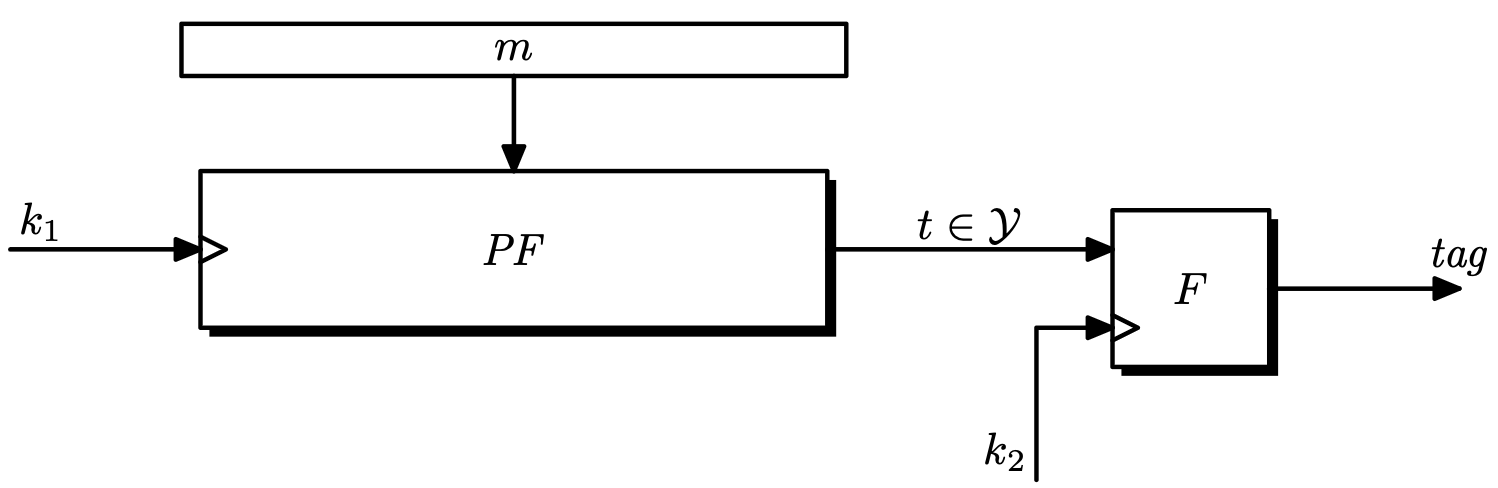
\includegraphics[width=0.65\linewidth]{figures/chapter6/fig4.png}
  \input{figures/chapter6/fig4.tex}
  \caption{加密 PRF 构造 $EF(k,m)$}
  \label{fig:6-4}
\end{figure}

我们声称,当 $PF$ 是 CBC 或级联中的任何一种构造时,$EF$ 都是一个安全的 PRF。更一般地,我们表明,只要 $PF$ 是一个\emph{可扩展的} PRF,$EF$ 就是安全的。可扩展性的定义如下:

\begin{definition}\label{def:6-4}
令 $PF$ 是一个定义在 $(\mathcal{K},\mathcal{X}^{\leq\ell},\mathcal{Y})$ 上的 PRF。如果对于所有的 $k\in\mathcal{K}$,$x,y\in\mathcal{X}^{\leq\ell-1}$ 和 $a\in\mathcal{X}$,我们都有:
\[
\text{if}\quad
PF(k,x)=PF(k,y)
\quad\text{then}\quad
PF(k,\;x\,\Vert\,a)=PF(k,\;y\,\Vert\,a)
\]
就称 $PF$ 是一个\textbf{可扩展 (extendable) PRF}。
\end{definition}

不难发现,CBC 和级联构造都是可扩展的 PRF。下面的定理将表明,如果 $PF$ 是一个可扩展的无前缀安全 PRF,$EF$ 就是一个安全的 PRF。

\begin{theorem}\label{theo:6-5}
令 $PF$ 是一个定义在 $(\mathcal{K}_1,\mathcal{X}^{\leq\ell+1},\mathcal{Y})$ 上的可扩展且无前缀安全的 PRF,其中 $|\mathcal{Y}|$ 是超多项式的,$\ell$ 是多项式约束的。令 $F$ 是一个定义在 $(\mathcal{K}_2,\mathcal{Y},\mathcal{T})$ 上的安全的 PRF。那么如式 \ref{eq:6-17} 中所定义的 $EF$ 是一个定义在 $(\mathcal{K}_1\times\mathcal{K}_2,\mathcal{X}^{\leq\ell},\mathcal{T})$ 上的安全的 PRF。
\begin{quote}
特别地,对于每个按照攻击游戏 \ref{game:4-2} 攻击 $EF$ 的 PRF 对手 $\mathcal{A}$,假设它最多能够向其挑战者发起 $Q$ 次查询,则必然存在一个按照攻击游戏 \ref{game:4-2} 攻击 $F$ 的 PRF 对手 $\mathcal{B}_1$ 和一个按照攻击游戏 \ref{game:4-2} 攻击 $PF$ 的无前缀 PRF 对手 $\mathcal{B}_2$,其中 $\mathcal{B}_1$ 和 $\mathcal{B}_2$ 都是围绕 $\mathcal{A}$ 的基本包装器,满足:
\end{quote}
\begin{equation}\label{eq:6-18}
{\rm PRF\mathsf{adv}}[\mathcal{A},EF]\leq {\rm PRF\mathsf{adv}}[\mathcal{B}_1,F]+{\rm PRF^{pf}\mathsf{adv}}[\mathcal{B}_2,PF]+\frac{Q^2}{2|\mathcal{Y}|}
\end{equation}
\end{theorem}

\noindent
在我们提供了必要的工具之后,我们将在下一章(\ref{subsec:7-3-1} 小节)证明定理 \ref{theo:6-5}。请注意,为了使 $EF$ 在长度不超过 $\ell$ 的输入上都是安全的 PRF,该定理要求 $PF$ 对于长为 $\ell+1$ 的输入是都无前缀安全的。

\begin{snote}[式 \ref{eq:6-18} 中的上界是严格的。]
虽然不是完全必要,但让我们假设 $\mathcal{Y}=\mathcal{T}$,$F$ 是一个分组密码,并且 $|\mathcal{X}|$ 不是非常小。这些假设将大大简化论证。我们下面展示一种攻击,它能在 $Q\approx\sqrt{|\mathcal{Y}|}$ 次查询之后以恒定概率攻破 $EF$。事实上,我们的攻击将攻破作为一个 MAC 的 $EF$。对手首先挑选 $Q$ 个随机输入 $x_1,\dots,x_Q\in\mathcal{X}^2$,并用这 $Q$ 个输入向其挑战者发起查询,以得到应答 $t_1,\dots,t_Q\in\mathcal{T}$。根据生日悖论(推论 \ref{cor:B-2}),对于任何固定的密钥 $k_1$,存在不同的索引 $i$ 和 $j$ 使得 $x_i\neq x_j$ 且 $PF(k_1,x_i)=PF(k_1,x_j)$ 的概率是恒定的。一方面,如果发生这样的碰撞,我们可以有效发现它,这是因为对于这样的一对索引,必有 $t_i=t_j$。另一方面,如果存在一对索引 $i$ 和 $j$ 使得 $t_i=t_j$,由于我们假设 $F$ 是一个分组密码,那么必然有 $PF(k_1,x_i)=PF(k_1,x_j)$。现在,假设 $x_i\neq x_j$ 且 $PF(k_1,x_i)=PF(k_1,x_j)$,由于 $PF$ 是可扩展的,那么对于任意 $a\in\mathcal{X}$,我们都有 $PF\big(k_1,\,(x_i\,\Vert\,a)\big)=PF\big(k_1,\,(x_j\,\Vert\,a)\big)$。因此,我们的对手可以获得 $x_i\,\Vert\,a$ 的 MAC 标签 $t$,而这个标签 $t$ 同时也是 $x_j\,\Vert\,a$ 的有效标签。推广这一攻击,我们就能很容易地证明式 \ref{eq:6-18} 中 ${Q^2}/{(2|\mathcal{Y}|)}$ 这一项的必要性。
\end{snote}

\subsection{ECBC 和 NMAC:用于变长输入的安全 PRF}

图 \ref{fig:6-5-a} 和 \ref{fig:6-5-b} 展示了对 CBC 和级联应用 $EF$ 构造的结果。

\begin{figure}
  \centering
  \subfigure[ECBC 构造 $\mathrm{ECBC}(k,m)$(加密CBC)]{
    \input{figures/chapter6/fig5-a.tex}
  	\label{fig:6-5-a}
  }
  
  \,
  
  \,
  
  \subfigure[NMAC 构造 $\mathrm{NMAC}(k,m)$(加密级联)]{
  	\input{figures/chapter6/fig5-b.tex}
  	\label{fig:6-5-b}
  }
  \caption{用于变长输入的安全 PRF}
\end{figure}

\subsubsection{加密 CBC PRF}

将 $EF$ 应用于 CBC 构造就能得到一个经典的 PRF(因而也是一个 MAC),称为\textbf{加密 CBC (encrypted-CBC)} 或 \textbf{ECBC}。这种 MAC 由 ANSI 标准化(见 \ref{sec:6-9} 节),并被广泛用于银行业。ECBC PRF 在 CBC 和最终的加密中使用相同的底层 PRF $F$。因此,ECBC 定义在 $(\mathcal{K}^2,\mathcal{X}^{\leq\ell+1},\mathcal{X})$ 上。

\begin{theorem}[ECBC 的安全性]\label{theo:6-6}
令 $F$ 是一个定义在 $(\mathcal{K},\mathcal{X},\mathcal{X})$ 上的安全 PRF。假设 $\mathcal{X}$ 是超多项式的,$\ell$ 是一个多项式约束的长度参数。那么 ECBC 是一个定义在 $(\mathcal{K}^2,\mathcal{X}^{\leq\ell+1},\mathcal{X})$ 上的安全 PRF。
\begin{quote}
特别地,对于每个按照攻击游戏 \ref{game:4-2} 攻击 ECBC 的 PRF 对手 $\mathcal{A}$,假设它最多能够向其挑战者发起 $Q$ 次查询,则必然存在两个按照攻击游戏 \ref{game:4-2} 攻击 $F$ 的 PRF 对手 $\mathcal{B}_1$ 和 $\mathcal{B}_2$,其中 $\mathcal{B}_1$ 和 $\mathcal{B}_2$ 都是围绕 $\mathcal{A}$ 的基本包装器,满足:
\end{quote}
\begin{equation}\label{eq:6-19}
{\rm PRF}\mathsf{adv}[\mathcal{A},{\rm ECBC}]\leq{\rm PRF}\mathsf{adv}[\mathcal{B}_1,F]+{\rm PRF}\mathsf{adv}[\mathcal{B}_2,F]+\frac{(Q(l+1))^2+Q^2}{2|\mathcal{X}|}
\end{equation}
\end{theorem}

\begin{proof}
根据定理 \ref{theo:6-3},CBC 显然是可扩展的,而且是一个无前缀安全的 PRF。因此,如果底层 PRF $F$ 是安全的,那么根据定理 \ref{theo:6-5},ECBC 也是一个安全的 PRF。
\end{proof}

定理 \ref{theo:6-5} 之后的论证表明,存在一个攻击者,在 $Q\approx\sqrt{|\mathcal{X}|}$ 次查询后,能以恒定优势破解该 PRF。回顾一下,对于 3DES,我们有 $\mathcal{X}=\{0,1\}^{64}$。因此,在大约 10 亿次(或者更准确地说, $2^{32}$ 次)查询之后,攻击者就能以恒定的概率破解 ECBC-3DES MAC。

\subsubsection{NMAC PRF}

将 $EF$ 应用于级联构造同样能得到一个 PRF(因而也是一个 MAC),称为\textbf{嵌套 MAC (Nested MAC)} 或 \textbf{NMAC}。这种 MAC 的一个变体由 IETF 标准化(见 \ref{subsec:8-7-2} 小节),并被广泛用于互联网协议中。

我们希望使用相同的底层 PRF $F$ 来构造级联和进行最终的加密。但不幸的是,级联的输出在 $\mathcal{K}$ 上,而 $F$ 的输入在 $\mathcal{X}$ 上。为了解决这个问题,我们需要将级联的输出嵌入到 $\mathcal{X}$ 中。更确切地说,我们假设 $|\mathcal{K}|\leq|\mathcal{X}|$,并且有一个可有效计算的双射 $g$,它能将 $\mathcal{K}$ 中的元素映射到 $\mathcal{X}$ 上。比如说,假设 $\mathcal{K}:=\{0,1\}^\kappa$,$\mathcal{X}:=\{0,1\}^n$,其中 $\kappa\leq n$。我们定义 $g(t):=t\,\Vert\,\mathsf{fpad}$,其中 $\mathsf{fpad}$ 是一串 $n-\kappa$ 比特的固定填充序列。这个 $\mathsf{fpad}$ 可以像一串 $0$ 一样简单。通过这种转换,所有的 NMAC 都可以由一个安全的 PRF $F$ 构造出来,就如图 \ref{fig:6-5-b} 所示。

\begin{theorem}[NMAC 的安全性]\label{theo:6-7}
令 $F$ 是一个定义在 $(\mathcal{K},\mathcal{X},\mathcal{K})$ 上的安全的 PRF,其中 $\mathcal{K}$ 可以嵌入到 $\mathcal{X}$ 中,那么 NMAC 就是一个定义在 $(\mathcal{K}^2,\mathcal{X}^{\leq\ell},\mathcal{K})$ 上的安全的 PRF。
\begin{quote}
特别地,对于每个按照攻击游戏 \ref{game:4-2} 攻击 NMAC 的 PRF 对手 $\mathcal{A}$,假设它最多能够向其挑战者发起 $Q$ 次查询,则必然存在两个按照攻击游戏 \ref{game:4-2} 攻击 $F$ 的 PRF 对手 $\mathcal{B}_1$ 和 $\mathcal{B}_2$,其中 $\mathcal{B}_1$ 和 $\mathcal{B}_2$ 都是围绕 $\mathcal{A}$ 的基本包装器,满足:
\end{quote}
\begin{equation}\label{eq:6-20}
{\rm PRF}\mathsf{adv}[\mathcal{A},{\rm NMAC}]\leq (Q(\ell+1))\cdot{\rm PRF}\mathsf{adv}[\mathcal{B}_1,F]+{\rm PRF}\mathsf{adv}[\mathcal{B}_2,F]+\frac{Q^2}{2|\mathcal{K}|}
\end{equation}
\end{theorem}

\begin{proof}
根据定理 \ref{theo:6-4},NMAC 显然是可扩展的,而且是一个无前缀安全的 PRF。因此,如果底层 PRF $F$ 是安全的,那么根据定理 \ref{theo:6-5},NMAC 也是一个安全的 PRF。
\end{proof}

\begin{snote}[ECBC 和 NMAC 都是流式 MAC。]
ECBC 和 NMAC 都可以用来认证 $\mathcal{X}^{\leq l}$ 上的变长消息。此外,我们并不需要提前知晓消息的长度。具有这种特性的 MAC 被称为\textbf{流式 MAC (streaming MAC)}。这一特性使得应用程序能够一次向 MAC 提供一个消息分组,并在任意位置决定消息是否结束。这对于像流媒体视频这样的应用很重要,因为在这种应用中,应用程序也无法预知消息的长度。

相比之下,一些 MAC 系统要求将消息长度预加到消息正文中(见 \ref{sec:6-6} 节)。这样的 MAC 在实践中更难使用,因为它们要求应用程序在开始计算 MAC 之前就确定消息的长度。
\end{snote}
\section{从无前缀安全 PRF 到完全安全 PRF(方法 2):无前缀编码}\label{sec:6-6}

将无前缀安全的 PRF 转换为安全 PRF 的另一种方法是对 PRF 的输入进行编码,使得没有任何一条编码后的输入是另一条的前缀。我们定义以下术语:
\begin{itemize}
	\item 如果 $S\subseteq\mathcal{X}^{\leq\ell}$ 中的任何元素都不是其他元素的前缀,我们就称 $S$ 是一个\textbf{无前缀集 (prefix-free set)}。例如,如果 $(x_1,x_2,x_3)$ 属于一个无前缀集 $S$,那么 $x_1$ 和 $(x_1,x_2)$ 都不在 $S$ 中。
	\item 令 $\mathcal{X}^{\leq\ell}_{_{>0}}$ 表示$\mathcal{X}$ 上所有长度不超过 $\ell$ 的非空序列的集合。如果映射 $pf$ 是一个单射(即一对一函数),且 $pf$ 的像是一个无前缀集,我们就称 $pf:\mathcal{M}\to\mathcal{X}^{\leq\ell}_{_{>0}}$ 是一个\textbf{无前缀编码 (prefix-free encoding)}。
\end{itemize}

令 $PF$ 是一个定义在 $(\mathcal{K},\mathcal{X}^{\leq\ell},\mathcal{Y})$ 上的无前缀安全 PRF,且 $pf:\mathcal{M}\to\mathcal{X}^{\leq\ell}_{_{>0}}$ 是一个无前缀编码。定义派生的 PRF $F$ 为:
\[
F(k,m):=PF(k,pf(m))
\]
那么 $F$ 定义在 $(\mathcal{K},\mathcal{M},\mathcal{Y})$ 上。于是,我们就可以得到下面的定理。

\begin{theorem}\label{theo:6-8}
如果 $PF$ 是一个无前缀安全的 PRF,$pf$ 是一个无前缀编码,那么 $F$ 是一个安全的 PRF。
\end{theorem}

\subsection{无前缀编码}\label{subsec:6-6-1}

为了使用定理 \ref{theo:6-8} 构造 PRF,我们介绍两种无前缀编码 $pf:\mathcal{M}\to\mathcal{X}^{\leq\ell}$。我们假设 $\mathcal{X}=\{0,1\}^n$,其中 $n$ 是某个整数。

\begin{snote}[方法 1:前置长度。]
设 $\mathcal{M}:=\mathcal{X}^{\leq\ell-1}$,并令 $m=(a_1,\dots,a_v)\in\mathcal{M}$。定义:
\[
pf(m):=(\langle v\rangle,a_1,\dots,a_v)\quad\in\mathcal{X}^{\leq\ell}_{_{>0}}
\]
其中 $\langle v\rangle\in\mathcal{X}$ 是 $v$ 的二进制表示,即 $m$ 的长度。我们假设 $\ell<2^n$,那么消息长度可以被编码为 $n$ 比特的二进制序列。

我们下面论证 $pf$ 是一个无前缀编码。首先,$pf$ 显然是一个单射。为了说明 $pf$ 的像是一个无前缀集,令 $pf(x)$ 和 $pf(y)$ 是 $pf$ 的像中的两个元素。如果 $pf(x)$ 和 $pf(y)$ 包含相同数量的分组,那么它们中的任何一个都不可能是另一个的真前缀。如果 $pf(x)$ 和 $pf(y)$ 包含不同数量的分组,它们就必须在第一个分组上就有所不同,此时它们也同样都不可能是另一个的真前缀。因此,$pf$ 是一个无前缀编码。

这种无前缀编码在实践中并不常用,因为这样所产生的 MAC 不是一个流式 MAC:使用这种 MAC 的应用程序必须提前把消息的长度承诺给 MAC。正如我们之前所说,这对于流媒体应用来说极不实用,因为在这种应用中,数据包的长度可能无法提前预知。
\end{snote}

\begin{snote}[方法 2:停止比特。]
设 $\mathcal{\bar{X}}:=\{0,1\}^{n-1}$,并令 $\mathcal{M}=\mathcal{\bar{X}}^{\leq\ell}_{_{>0}}$。对于 $m=(a_1,\dots,a_v)\in\mathcal{M}$,定义:
\[
pf(m):=\big((a_1\,\Vert\,0),\,(a_2\,\Vert\,0),\,\dots,\,(a_{v-1}\,\Vert\,0),\,(a_v\,\Vert\,1)\big)\quad\in\mathcal{X}^{\leq\ell}_{_{>0}}
\]
显然,$pf$ 是一个单射。为了说明 $pf$ 的像是一个无前缀集,令 $pf(x)$ 和 $pf(y)$ 是 $pf$ 的像中的两个元素。设 $v$ 是 $pf(x)$ 中分组的数量。如果 $pf(y)$ 包含 $v$ 个或更少的分组,那么 $pf(x)$ 必然不是 $pf(y)$ 的真前缀。如果 $pf(y)$ 包含多于 $v$ 个分组,那么 $pf(y)$ 中的 $v$ 号分组以 $0$ 结束,而 $pf(x)$ 中的 $v$ 号分组以 $1$ 结束。因此,$pf(x)$ 和 $pf(y)$ 在 $v$ 号分组上有所不同,所以 $pf(x)$ 不是 $pf(y)$ 的真前缀。

这种无前缀编码所产生的 MAC 是一个流式 MAC。然而,这种编码使 MAC 的长度增加了 $v$ 比特。当使用 CBC 或级联计算一个长消息的 MAC 时,这种编码将导致对底层 PRF(比如 AES)的额外计算。相对地,\ref{sec:6-5} 节中介绍的加密 PRF 方法只增加了一次对底层 PRF 的计算。例如,使用 ECBC-AES 和 $pf$ 对一兆字节 ($2^{20}$ 字节) 的消息计算 MAC,除了加密 PRF 方法所需要的,还需要对 AES 进行额外的 $511$ 次评估。在实践中,情况甚至可能更糟。由于计算机更喜欢字节对齐的数据,我们很可能需要在每个分组中附加一整个字节,而不是仅仅一个比特。那么,使用 ECBC-AES 和 $pf$ 对一兆字节的消息计算 MAC,将导致比加密 PRF 方法多出 $4096$ 次 AES 的计算,大约多 $6\%$ 的开销。
\end{snote}
\section{从无前缀安全PRF到完全安全PRF(方法3):CMAC}\label{sec:6-7}

上一节中介绍的两种无前缀编码方法都有问题。第一种方法产生的 MAC 是非流式的,而第二种方法对于长的消息需要对底层的 PRF 进行更多的计算。我们可以将无前缀编码进行随机化处理来进一步地改进设计。我们下面建立一个流式且安全的 PRF,除了底层的无前缀安全 PRF 之外,该设计不会引入任何额外的开销。图 \ref{fig:6-6} 展示了这样的 MAC,它比从加密 PRF 或者确定性编码得到的 MAC 都要优秀。这种方法被用于 NIST 的一种 MAC 标准,称为 CMAC,我们将在 \ref{sec:6-10} 节中介绍它。

\begin{figure}
  \centering
  \subfigure[应用于 CBC 的 $rpf$]{
    \input{figures/chapter6/fig6-a.tex}
  }
  
  \,
  
  \,
  
  \subfigure[应用于级联的 $rpf$]{
    \input{figures/chapter6/fig6-b.tex}
  }
  \caption{使用随机无前缀编码的安全 PRF}
  \label{fig:6-6}
\end{figure}

首先,为了叙述方便,我们引入一些符号:

\begin{definition}\label{def:6-5}
对于两个序列 $x,y\in\mathcal{X}^{\leq\ell}$,如果 $x$ 是 $y$ 的一个前缀,或者 $y$ 是 $x$ 的一个前缀,我们就记 $x\sim y$。
\end{definition}

\begin{definition}\label{def:6-6}
令 $\epsilon$ 是一个实数,满足 $0\leq\epsilon\leq1$。一个\textbf{随机性 $\epsilon$-无前缀 (randomized $\epsilon$-prefix-free)} 编码是一个函数 $rpf:\mathcal{K}\times\mathcal{M}\to\mathcal{X}^{\leq\ell}_{_{>0}}$,使得对于任意 $m_0,m_1\in\mathcal{M}$,$m_0\neq m_1$,我们都有:
\[
\Pr\big[rpf(k,m_0)\sim rpf(k,m_1)\big]\leq\epsilon
\]
这里的概率取决于从 $\mathcal{K}$ 中随机选取的 $k$。
\end{definition}

\noindent
请注意,$rpf(k,\cdot)$ 的像不需要是一个无前缀集合。然而,在不知道 $k$ 的情况下,很难找到 $m_0,m_1\in\mathcal{M}$ 使得 $rpf(k,m_0)$ 是 $rpf(k,m_1)$ 的真前缀(或者反之)。函数 $rpf(k,\cdot)$ 甚至不需要是一个单射。

\begin{snote}[一个简单的 $rpf$。]
令 $\mathcal{K}:=\mathcal{X}$,$\mathcal{M}:=\mathcal{X}^{\leq\ell}_{_{>0}}$。定义:
\[
rpf(k,(a_1,\dots,a_v))=(a_1,\dots,a_{v-1},(a_v\oplus k))\in\mathcal{X}^{\leq\ell}_{_{>0}}
\]
不难发现 $rpf$ 是一个随机性 $({1}/{|\mathcal{X}|})$-无前缀编码。令 $m_0,m_1\in\mathcal{M}$,并且 $m_0\neq m_1$。假设 $|m_0|=|m_1|$。那么很明显,对于所有 $k$ 的选择,$rpf(k,m_0)$ 和 $rpf(k,m_1)$ 都是长度相同的不同序列,所以两者都不可能是对方的前缀。接下来,假设 $|m_0|<|m_1|$。如果 $v:=|rpf(k,m_0)|$,那么很显然,当且仅当:
\[
m_0[v-1]\oplus k=m_1[v-1]
\]
时,$rpf(k,m_0)$ 才是 $rpf(k,m_1)$ 的一个真前缀。然而,在随机选择 $k$ 的情况下,上式成立的概率是 ${1}/{|\mathcal{X}|}$,这符合要求。最后,对于 $|m_0|>|m_1|$ 的情况,可以用一个对称的论证来处理。
\end{snote}

\begin{snote}[使用 $rpf$。]
令 $PF$ 是一个定义在 $(\mathcal{K},\mathcal{X}^{\leq\ell},\mathcal{Y})$ 上的无前缀安全 PRF,且 $rpf:\mathcal{K}_1\times\mathcal{M}\to\mathcal{X}^{\leq\ell}_{_{>0}}$ 是一个随机化的无前缀编码。定义派生出的 PRF $F$ 为:
\begin{equation}\label{eq:6-21}
F\big((k,k_1),\,m\big):=PF\big(k,\,rpf(k_1,m)\big)
\end{equation}
那么,$F$ 就定义在 $(\mathcal{K}\times\mathcal{K}_1,\mathcal{M},\mathcal{Y})$ 上。我们可以得到以下定理,它与定理 \ref{theo:6-8} 类似。
\end{snote}

\begin{theorem}\label{theo:6-9}
如果 $PF$ 是一个无前缀安全的 PRF,$\epsilon$ 可忽略不计,并且 $rpf$ 是一个随机性 $\epsilon$-无前缀编码,则式 \ref{eq:6-21} 中定义的 $F$ 是一个安全的 PRF。
\begin{quote}
特别地,对于每个按照攻击游戏 \ref{game:4-2} 攻击 $F$ 的 PRF 对手 $\mathcal{A}$,假设它最多能够向其挑战者发起 $Q$ 次查询,则必然存在两个按照攻击游戏 \ref{game:4-2} 攻击 $PF$ 的无前缀 PRF 对手 $\mathcal{B}_1$ 和 $\mathcal{B}_2$,使得 $\mathcal{B}_1$ 和 $\mathcal{B}_2$ 都是围绕 $\mathcal{A}$ 的基本包装器,满足:
\end{quote}
\begin{equation}\label{eq:6-22}
{\rm PRF}\mathsf{adv}[\mathcal{A},F]\leq
{\rm PRF^{pf}}\mathsf{adv}[\mathcal{B}_1,PF]+{\rm PRF^{pf}}\mathsf{adv}[\mathcal{B}_2,PF]+{Q^2\epsilon}/{2}
\end{equation}
\end{theorem}

\begin{proof}[证明思路]
如果对手对于 $F$ 的输入集能够产生对于 $PF$ 的无前缀输入集,那么对手看到的就只是一些看起来很随机的输出。此外,如果对手看到的是随机的输出,它就没有得到关于 $rpf$ 的密钥 $k_1$ 的任何有效信息,这就确保 $PF$ 的输入集确实(以压倒性的概率)是无前缀的。不幸的是,上述思路会导致一个循环论证。我们将在下面的证明中介绍打破这种循环论证的方法。
\end{proof}

\begin{proof}
不失一般性,我们假设 $\mathcal{A}$ 从未发出过两次相同的查询。我们将证明组织成由三个游戏构成的一个序列。对于 $j=0,1,2$,我们令 $W_j$ 是 $\mathcal{A}$ 在游戏 $j$ 结束时输出 $1$ 的事件。

\vspace{5pt}

\noindent\textbf{游戏$\mathbf{0}$}。
在 PRF 攻击游戏 \ref{game:4-2} 的实验 $0$ 中,挑战者就 $F$ 进行如下操作:

\vspace{5pt}

\hspace*{5pt} 选取 $k\overset{\rm R}\leftarrow\mathcal{K}$,$k_1\overset{\rm R}\leftarrow\mathcal{K}_1$\\
\hspace*{26pt} 当从 $\mathcal{A}$ 处收到签名查询 $m_i\in\mathcal{M}$ ($i=1,2,\dots$) 时:\\
\hspace*{50pt} 令 $x_i\leftarrow rpf(k_1,m_i)\in\mathcal{X}^{\leq\ell}_{_{>0}}$\\
\hspace*{50pt} 令 $y_i\leftarrow PF(k,x_i)$\\
\hspace*{50pt} 将 $y_i$ 发送给 $\mathcal{A}$

\vspace{5pt}

\noindent\textbf{游戏$\mathbf{1}$}。
我们修改游戏 $0$ 中的挑战者,以确保对 $PF$ 的所有查询都是无前缀的。回顾一下符号 $x\sim y$,它表示 $x$ 是 $y$ 的前缀,或者 $y$ 是 $x$ 的前缀。

\vspace{5pt}

\hspace*{5pt} 选取 $k\overset{\rm R}\leftarrow\mathcal{K}$,$k_1\overset{\rm R}\leftarrow\mathcal{K}_1$,$r_1,\dots,r_Q\overset{\rm R}\leftarrow\mathcal{Y}$\\
\hspace*{26pt} 当从 $\mathcal{A}$ 处收到签名查询 $m_i\in\mathcal{M}$ ($i=1,2,\dots$) 时:\\
\hspace*{50pt} 令 $x_i\leftarrow rpf(k_1,m_i)\in\mathcal{X}^{\leq\ell}_{_{>0}}$\\
\hspace*{1pt} ($1$)
\hspace*{28.5pt} 如果存在某个 $j<i$ 使得 $x_i\sim x_j$:\\
\hspace*{75pt} 则令 $y_i\leftarrow r_i$\\
\hspace*{1pt} ($2$)
\hspace*{53.5pt} 否则令 $y_i\leftarrow PF(k,x_i)$\\ % 21.5pt deducted
\hspace*{50pt} 将 $y_i$ 发送给 $\mathcal{A}$

\vspace{5pt}

\noindent
令 $Z_1$ 为在游戏 $1$ 中的某个时刻,行 ($1$) 中的条件成立的事件。显然,在事件 $Z_1$ 发生之前,游戏 $1$ 和游戏 $2$ 的进程是完全相同的;特别地,当且仅当 $W_1\land\bar{Z}_1$ 发生时,$W_0\land\bar{Z}_1$ 才会发生。因此,基于差分引理(定理 \ref{theo:4-7}),我们得到:
\begin{equation}\label{eq:6-23}
\big\lvert\Pr[W_1]-\Pr[W_0]\big\rvert\leq\Pr[Z_1]
\end{equation}
不幸的是,在这一点上,我们还不能完全约束 $\Pr[Z_1]$。当分析进行到这一阶段时,我们还不能说明对 $PF$ 的评估在行 ($2$) 不会泄漏关于 $k_1$ 的信息。这些信息可能可以帮助 $\mathcal{A}$ 促使事件 $Z_1$ 发生。这就是我们上面提到的循环论证的问题。为了客服这一问题,我们把对 $Z_1$ 的分析推迟到下一个游戏。

\vspace{5pt}

\noindent\textbf{游戏$\mathbf{2}$}。
现在,与往常一样,我们打出``PRF牌",用一个真随机函数取代函数 $PF(k,\cdot)$。这是合理的,因为从构造上来看,在游戏 $1$ 中,$PF(k,\cdot)$ 的输入集是无前缀的。为了实现这一修改,我们可以简单地将标有 ($2$) 的一行替换为:

\vspace{5pt}

\hspace*{-19pt} ($2$)
\hspace*{53.5pt} 否则令 $y_i\leftarrow PF(k,x_i)$

\vspace{5pt}

\noindent
做了这样的修改后,我们可以看到,无论行 ($1$) 中的条件是否成立,$y_i$ 都会被分配一个随机值 $r_i$。

现在,令 $Z_2$ 表示在游戏 $2$ 中的某个时刻,行 ($1$) 中的条件成立的事件。不难得到,对于有效的无前缀 PRF 对手 $\mathcal{B}_1$ 和 $\mathcal{B}_2$,有:
\begin{equation}\label{eq:6-24}
\big\lvert\Pr[Z_1]-\Pr[Z_2]\big\rvert\leq{\rm PRF^{pf}}\mathsf{adv}[\mathcal{B}_1,F]
\end{equation}
和:
\begin{equation}\label{eq:6-25}
\big\lvert\Pr[W_1]-\Pr[W_2]\big\rvert\leq{\rm PRF^{pf}}\mathsf{adv}[\mathcal{B}_2,F]
\end{equation}
成立。这两个对手基本上是一样的,只是当行 ($1$) 中的条件成立时,$\mathcal{B}_1$ 就会输出 $1$,而 $\mathcal{B}_2$ 则会输出 $\mathcal{A}$ 所输出的任何结果。

此外,在游戏 $2$ 中,$k_1$ 的值显然与 $\mathcal{A}$ 的查询无关,因此利用 $rpf$ 的 $\epsilon$-无前缀属性,根据联合约束,我们可以得到:
\begin{equation}\label{eq:6-26}
\Pr[Z_2]\leq{Q^2\epsilon}/{2}
\end{equation}

最后,对 $\mathcal{A}$ 来说,游戏 $2$ 完美地模拟了 ${\rm Funs}[\mathcal{M},\mathcal{Y}]$ 中的一个随机函数。因此,游戏 $2$ 与就 $F$ 的攻击游戏 \ref{game:4-2} 中的实验 $1$ 是相同的,因此:
\begin{equation}\label{eq:6-27}
\big\lvert\Pr[W_0]-\Pr[W_2]\big\rvert={\rm PRF}\mathsf{adv}[\mathcal{A},F]
\end{equation}
现在,结合式 \ref{eq:6-23},\ref{eq:6-24},\ref{eq:6-25},\ref{eq:6-26} 和 \ref{eq:6-27},该定理得证。
\end{proof}
\section{将按分组 PRF 转化为按比特 PRF}\label{sec:6-8}

到目前为止,我们为 $\mathcal{X}^{\leq\ell}$ 上的变长输入构建了一些 PRF。通常 $\mathcal{X}=\{0,1\}^n$,其中 $n$ 是底层 PRF 的分组大小,CBC 或者级联构造都基于该参数构建(例如,对于 AES,$n=128$)。迄今为止,我们所介绍的所有 MAC 都被设计用来验证长度为 $n$ 比特的倍数的消息。

在本节中,我们将展示如何将这些 PRF 转换为针对任意长度消息的 PRF。也就是说,给定一个针对 $\mathcal{X}^{\leq\ell}$ 上的消息的 PRF,我们想要构建一个针对 $\{0,1\}^{\leq n\ell}$ 上的消息的 PRF。

令 $F$ 是一个接受 $\mathcal{X}^{\leq l+1}$ 中输入的 PRF。令 $inj:\{0,1\}^{\leq n\ell}\to\mathcal{X}^{\leq\ell+1}$ 是一个单射(即一对一)函数。定义派生出的 PRF $F_{\rm bit}$ 为:
\[
F_{\rm bit}(k,x):=F(k,\,inj(x))
\]
于是,我们可以得到下面的一个三段式定理。

\begin{theorem}\label{theo:6-10}
如果 $F$ 是一个定义在 $(\mathcal{K},\mathcal{X}^{\leq\ell+1},\mathcal{Y})$ 上的安全的 PRF,则 $F_{\rm bit}$ 是一个定义在 $(\mathcal{K},\{0,1\}^{\leq n\ell},\mathcal{Y})$ 上的安全的 PRF。
\end{theorem}

\begin{figure}
  \centering
  \input{figures/chapter6/fig7.tex}
  \caption{一个单射函数 $inj:\{0,1\}^{\leq n\ell}\to\mathcal{X}^{\leq\ell+1}$}
  \label{fig:6-7}
\end{figure}

\begin{snote}[一个单射函数。]
对于 $\mathcal{X}:=\{0,1\}^n$,一个从 $\{0,1\}^{\leq n\ell}$ 到 $\mathcal{X}^{\leq\ell+1}$ 的单射 $inj$ 的标准例子如下。如果输入消息的长度不是 $n$ 的倍数,那么 $inj$ 会添加 $100\dots00$ 来填充消息,使得它的长度成为 $n$ 的倍数,图 \ref{fig:6-7} 以图像的形式直观地刻画了这一点。更准确地说,该函数的工作原理如下:

\vspace{5pt}

\hspace*{5pt} 输入:$m\in\{0,1\}^{\leq nl}$

\vspace{3pt}

\hspace*{5pt} 令 $u\leftarrow|m|\;\mathrm{mod}\;n$,$m'\leftarrow m\,\Vert\,1\,\Vert\,0^{n-u-1}$\\
\hspace*{26pt} 输出 $m'$ 作为 $n$ 比特消息分组的一个序列

\vspace{5pt}

\noindent
为了说明 $inj$ 是一个单射,我们先表明它是可逆的。给定 $y\leftarrow inj(m)$,从右到左扫描 $y$,并删除所有 $0$ 和初次见到的 $1$,那么剩下的序列就是 $m$。

\vspace{5pt}

一个常见的错误就是用一个全 $0$ 的填充序列将给定的消息填充成分组长度的倍数。这样的映射并不是单射,并且会产生一个不安全的 MAC:对于任何长度不是分组长度的整数倍的消息 $m$,其 MAC 也是 $m\,\Vert\,0$ 的一个有效 MAC。因此,这样的 MAC 容易受到存在性伪造攻击。
\end{snote}

\begin{snote}[单射函数必会扩充。]
当我们把一个 $n$ 比特的单分组消息输入 $inj$ 时,该函数必须要增加一个``假"分组,并输出一个两分组消息。这对于那些主要以单分组消息为对象的应用来说是很不利的。当使用 CBC 或级联构造时,假分组迫使签名者和验证者对于每条消息都要评估两次底层的 PRF,就算所有的消息本身都只有一个分组。结果就是,所有参与方的计算量都被翻倍了。

因此,我们很自然地想要找到一个不需要添加假分组的单射函数。但不幸的是,这样的函数是不存在的,因为集合 $\{0,1\}^{\leq n\ell}$ 比集合 $\mathcal{X}^{\leq\ell}$ 要大。因此,所有的单射函数都必须要在输出中添加一个``假"分组。

我们将在 \ref{sec:6-10} 节介绍的 CMAC 构造为这个问题提供了一个优雅的解决方案。CMAC 通过使用一个\emph{随机化的}单射函数来避免添加假分组。
\end{snote}
\section{案例研究:ANSI CBC-MAC}\label{sec:6-9}

当使用 PRF 构建 MAC 时,实现者经常会只输出 PRF 输出的 $w$ 个最高有效比特来缩短最终得到的标签。练习 \ref{exer:4-4} 表明,将一个安全的 PRF 的输出截短并不会影响其作为 PRF 的安全性。但是,这种截短会影响派生的 MAC。定理 \ref{theo:6-2} 表明,$w$ 越小,MAC 的安全性就越低。特别是,该定理在具体的安全边界中包含一个 $1/2^w$ 的误差项。

两个 ANSI 标准(ANSI X9.9 和 ANSI X9.19)和两个 ISO 标准(ISO 8731-1 和 ISO/IEC 9797)指定了 ECBC 的几个变体,它们使用 DES 作为底层的 PRF,提供消息认证的功能。这些标准都截短了 ECBC-DES 的最终 $64$ 比特输出,只使用输出的最左边 $w$ 个比特,其中 $w=32$,$48$ 或 $64$。这种设计以降低安全性为代价,减少了标签的长度。

ANSI 的两个 CBC-MAC 标准都指定了一个填充方案,用于填充长度不是 DES 或者 AES 分组长度整数倍的消息。该填充方案与 \ref{sec:6-8} 节中描述的函数 $inj$ 相同。在签署消息和验证消息-标签对时,使用的填充方案都应当是相同的。
\section{CMAC}
\section{PMAC:一种并行的 MAC}\label{sec:6-11}

迄今为止,我们所介绍的所有 MAC 构造,包括 ECBC,CMAC 和 NMAC,本质上都是串行性的。也就是说,在第 $i-1$ 个分组的计算完成之前,无论如何都无法计算第 $i$ 个分组。这就使得我们很难利用硬件的并行性或流水线来加速 MAC 的生成和认证。在本节中,我们将介绍一种非常适合并行架构的安全 MAC,称作 PMAC。更具体地,我们将介绍一种名为 $\rm PMAC_0$ 的算法,因为它更容易描述。

令 $F_1$ 是一个定义在 $(\mathcal{K}_1,\mathbb{Z}_p,\mathcal{Y})$ 上的 PRF,其中 $p$ 是一个素数,$\mathcal{Y}:=\{0,1\}^n$。令 $F_2$ 是一个定义在 $(\mathcal{K}_2,\mathcal{Y},\mathcal{Z})$ 上的 PRF。

下面,我们构建一个新的 PRF,称作 $\rm PMAC_0$,它将一个密钥和一条 $\mathbb{Z}^{\leq\ell}_p$ 上的消息作为输入,输出 $\mathcal{Z}$ 上的一个元素。一个 $\rm PMAC_0$ 的密钥由 $k\in\mathbb{Z}_p$,$k_1\in\mathcal{K}_2$ 和 $k_2\in\mathcal{K}_2$ 组成。$\rm PMAC_0$ 构造的工作原理如下:

\vspace{5pt}

\hspace*{5pt} 输入:$m=(a_1,\dots,a_v)\in\mathbb{Z}^v_p$,其中 $0\leq v\leq\ell$,以及\\
\hspace*{75pt} 密钥 $\vec{k}=(k,k_1,k_2)$,其中 $k\in\mathbb{Z}_p$,$k_1\in\mathcal{K}_1$,$k_2\in\mathcal{K}_2$\\
\hspace*{26pt} 输出:$\mathcal{Z}$ 中的一个标签

\vspace{5pt}

\hspace*{5pt} ${\rm PMAC}_0(\vec{k},m)$:\\
\hspace*{50pt} 令 $t\leftarrow 0^n\in\mathcal{Y}$,$mask\leftarrow 0\in\mathbb{Z}_p$\\
\hspace*{50pt} 对于 $i=1,\dots,v$:\\
\hspace*{75pt} 令 $mask\leftarrow mask+k$ \quad\quad // $mask=i\cdot k\in\mathbb{Z}_p$\\
\hspace*{75pt} 令 $r\leftarrow a_i+mask$ \quad\quad\quad\; // $r=a_i+i\cdot k\in\mathbb{Z}_p$\\
\hspace*{75pt} 令 $t\leftarrow t\oplus F_1(k_1,r)$\\
\hspace*{50pt} 输出 $F_2(k_2,t)$

\vspace{5pt}

\noindent
在评估 $F_1$ 之前,主循环将掩码 $k,2k,3k,\dots$ 加到每个消息分组上。在一个串行设备上,这需要在每轮迭代中进行两次模 $p$ 加法。而在并行设备上,每个处理器都可以独立计算 $a_i+i\cdot k$,然后将其应用到 $F_1$ 上,如图 \ref{fig:6-9} 所示。

$\rm PMAC_0$ 是一个安全的 PRF,因此对于长的消息来说,$\rm PMAC_0$ 可以作为一个安全的 MAC。根据下一章的定理 \ref{theo:7-7},我们很容易给出它的安全性证明。现在,我们先说明该定理,并将对它的证明留到 \ref{subsec:7-3-3} 小节。

\begin{figure}
  \centering
  \input{figures/chapter6/fig9.tex}
  \caption{$\rm PMAC_0$ 构造}
  \label{fig:6-9}
\end{figure}

\begin{theorem}\label{theo:6-11}
如果 $F_1$ 和 $F_2$ 都是安全的 PRF,且 $|\mathcal{Y}|$ 和素数 $p$ 都是超多项式的,那么 $\rm PMAC_0$ 对于任何多项式约束的 $\ell$ 都是安全的 PRF。
\begin{quote}
特别地,对于每个按照攻击游戏 \ref{game:4-2} 攻击 $\rm PMAC_0$ 的 PRF 对手 $\mathcal{A}$,假设它最多能够向其挑战者发起 $Q$ 次查询,则必然存在两个 PRF 对手 $\mathcal{B}_1$ 和 $\mathcal{B}_2$,其中 $\mathcal{B}_1$ 和 $\mathcal{B}_2$ 都是围绕 $\mathcal{A}$ 的基本包装器,满足:
\end{quote}
\begin{equation}\label{eq:6-28}
{\rm PRF}\mathsf{adv}[\mathcal{A}, {\rm PMAC_0}]\leq{\rm PRF}\mathsf{adv}[\mathcal{B}_1,F_1]+{\rm PRF}\mathsf{adv}[\mathcal{B}_2,F_2]+\frac{Q^2}{2|\mathcal{Y}|}+\frac{Q^2\ell^2}{2p}
\end{equation}
\end{theorem}

当使用 $\rm PMAC_0$ 时,我们要把输入消息切分成多个分组,其中的每个分组都是 $\mathbb{Z}_p$ 中的元素。在实践中,这是很不方便的。相对地,将每条消息切分成 $\{0,1\}^n$ 中的 $n$ 比特序列就要容易得多。接下来介绍的一个更好的并行 MAC 构造,正是通过使用有限域 ${\rm GF}(2^n)$ 代替 $\mathbb{Z}_p$ 实现的。这是一个很好的例子,能够说明为什么有限域 ${\rm GF}(2^n)$ 在密码学中如此重要。出于安全考虑,我们经常需要将计算定义在某个域上,但是像 $\mathbb{Z}_p$ 这样的素阶有限域在实践中总是不太方便。${\rm GF}(2^n)$ 相对来说就要好很多,它上面的算术运算更快,还能很自然地让我们对 $n$ 比特序列进行操作。

\begin{snote}[比 $\rm PMAC_0$ 更好的 PMAC。]
尽管 $\rm PMAC_0$ 非常适合用在并行硬件上,但它仍然有改进空间。事实上,还有一些比 $\rm PMAC_0$  更优秀的实现,包括 PMAC 和 XECB,它们都是可并行的。具体地,PMAC 相对 $\rm PMAC_0$ 来说有如下的改进:
\begin{itemize}
	\item PMAC 使用有限域 ${\rm GF}(2^n)$ 上的算术运算,而不是 $\mathbb{Z}_p$。${\rm GF}(2^n)$ 中的元素可以表示为 $n$ 比特长的序列,域上的加法就是按位异或。正因如此,PMAC 实际上只是使用了 $F_1=F_2=F$,其中 $F$ 是定义在 $(\mathcal{K},\mathcal{Y},\mathcal{Y})$ 上的一个 PRF。PMAC 的输入空间由 $\mathcal{Y}=\{0,1\}^n$ 中的元素序列组成,而不是 $\mathbb{Z}_p$ 中的元素。
	\item PMAC 的第 $i$ 分组的掩码被定义为 $\gamma_i\cdot k$,其中 $\gamma_1,\gamma_2,\dots$ 是 ${\rm GF}(2^n)$ 中的固定常数。乘法也定义在 ${\rm GF}(2^n)$ 上。$\gamma_i$ 是经过特别选取的,为的是保证从 $\gamma_i\cdot k$ 计算 $\gamma_{i+1}\cdot k$ 成本很低。
	\item PMAC 的密钥 $k$ 是由 $k\leftarrow F(k_1,0^n)$ 派生而来的,并且令 $k_2\leftarrow k_1$。因此,PMAC 使用的密匙比 $\rm PMAC_0$ 的更短。
	\item PMAC 使用一个技巧来保存 $F$ 的一个应用。
	\item PMAC 使用 CMAC $rpf$ 的一个变体来提供按位 PRF。
\end{itemize}
结果就是,PMAC 在串行设备上与 ECBC 和 NMAC 的效率相近,但在并行或流水线设备上有更好的性能。PMAC 在本章所介绍的所有 PRF 中是最优秀的,它在各种计算机结构上都能很好地工作,对长消息和短消息都很有效。
\end{snote}

\begin{snote}[$\rm PMAC_0$ 是增量的。]
假设 Bob 为某一条长消息 $m$ 计算了标签 $t$,一段时间后他改变了 $m$ 中的一个分组,想要重新计算这条新消息 $m'$ 的标签。当使用 CBC-MAC 时,现在的标签 $t$ 对于新的计算是毫无用处的——Bob 必须从头开始计算 $m'$ 的新标签。但使用 $\rm PMAC_0$ 时,情况就会有很大的改观。假设用于构造 $\rm PMAC_0$ 的 PRF $F_2$ 是一个分组密码,比如 AES,令 $D$ 为该分组密码的解密算法。令 $m'$ 是将 $m$ 的第 $i$ 个分组从 $a_i$ 修改为 $a_i'$ 后得到的新消息。那么,我们很容易由 $m$ 的标签 $t:={\rm PMAC_0}(k,m)$ 推导出 $m'$ 的新标签 $t':={\rm PMAC_0}(k,m')$,方法如下:

\vspace{5pt}

\hspace*{5pt} 令 $t_1\leftarrow D(k_2,t)$\\
\hspace*{26pt} 令 $t_2\leftarrow t_1\oplus F_1(k_1,\;a_i+i\cdot k)\oplus F_1(k_1,\;a_i'+i\cdot k)$\\
\hspace*{26pt} 令 $t'\leftarrow F_2(k_2,t_2)$

\vspace{5pt}

\noindent
因此,给定某个长消息 $m$ 的标签(以及 MAC 的密钥),我们很容易推导出对 $m$ 进行局部修改后的新标签。具有这种性质的 MAC 被称作是\textbf{增量的(incremental)}。我们上面标明,使用分组密码实现的 $\rm PMAC_0$ 是增量的。
\end{snote}
\section{一个有趣的应用:在加密数据上进行搜索}

待写。
\section{笔记}
\section{练习}
\chapter{来自通用哈希的消息完整性}

在上一章中,我们展示了如何使用安全的 PRF 构建安全的 MAC。特别地,我们讨论了 ECBC、NMAC 和 $\mathrm{PMAC}_0$ 等几个构造。我们描述了这些 MAC 的安全定理,但将其证明留到了本章。

在本章中,我们将描述一个使用哈希函数构建 MAC 的一般范式。我们所说的\textbf{哈希函数 (hash function)} 一般是指能将某个大集合 $\mathcal{M}$ 中的输入映射到 $\mathcal{T}$ 中的短输出的函数 $H$。$\mathcal{T}$ 中的元素通常被称为\textbf{消息摘要 (message digest)}。本章中所使用的带密钥的哈希函数,还需要将一个密钥 $k$ 作为输入。

从更高的层次上看,由哈希函数构建的 MAC 分两步工作。首先,我们使用哈希函数将消息 $m$ 哈希成一个简短的摘要 $t$。然后,我们将摘要 $t$ 应用到一个 PRF 上,如图 \ref{fig:7-1} 所示。

正如我们将要看到的,ECBC、NMAC 和 $\mathrm{PMAC}_0$ 都是这种``先哈希后 PRF" 范式的实例。例如,对于 ECBC 来说(见图 \ref{fig:6-5-a}),我们把 CBC 函数作为一个哈希函数,它将长的输入哈希成短的摘要。最后,我们使用一个 PRF 和密钥 $k_2$ 来处理哈希生成的摘要。先哈希后 PRF 范式让我们能够直接和相当容易地推导出 ECBC、NMAC 和 $\mathrm{PMAC}_0$ 的安全性。

先哈希后 PRF 范式是非常通用的,它让我们能够使用各种哈希函数建立新的 MAC。其中的一些哈希函数非常快,所产生的 MAC 也比上一章介绍的要更加高效。

\begin{figure}
  \centering
  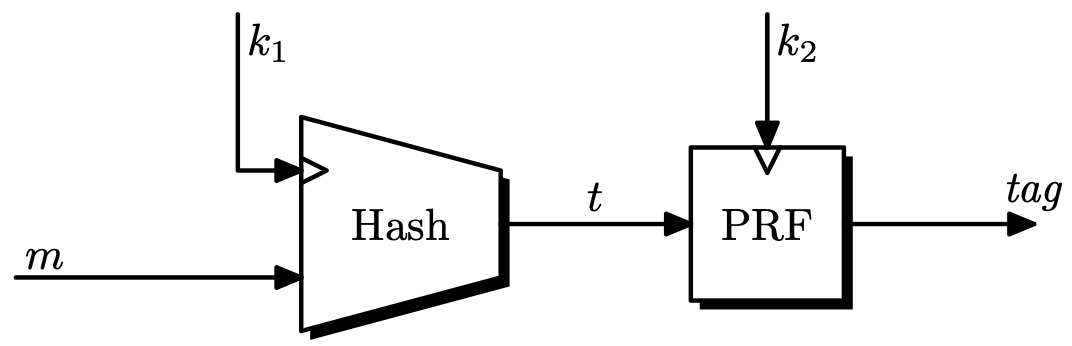
\includegraphics[width=0.45\linewidth]{figures/chapter7/fig1.png}
  \caption{先哈希后 PRF 范式}
  \label{fig:7-1}
\end{figure}

\section{通用哈希函数}
\section{构造 UHF}\label{sec:7-2}

构建良好的通用哈希函数(UHF)的挑战是构建一个使用短密钥实现小碰撞概率的函数。最理想的情况是密钥的长度不取决与被哈希的消息的长度。我们下面给出三种构造。第一种构造是基于算术模运算和多项式的一个\emph{统计性} UHF 的优雅构造。第二种构造基于 \ref{sec:6-4} 节中介绍的 CBC 和级联函数。我们表明,这两者都是\emph{计算性} UHF。第三种构造基于 \ref{sec:6-11} 节中介绍的 $\mathrm{PMAC}_0$。

\subsection{构造 1:使用多项式构建 UHF}\label{subsec:7-2-1}

我们从一个使用多项式模一个素数的 UHF 构造开始。令 $\ell$ 是一个(多项式边界的)长度参数,并令 $p$ 是一个素数。我们定义一个哈希函数 $H_{\rm poly}$,它能将一条消息 $m\in\mathbb{Z}^{\leq\ell}_p$ 哈希为一个单一元素 $t\in\mathbb{Z}_p$。其密钥空间为 $\mathcal{K}:=\mathbb{Z}_p$。

令 $m$ 是一条消息,即 $m=(a_1,\dots,a_v)\in\mathbb{Z}^{\leq\ell}_p$,其中 $0\leq v\leq\ell$。令 $k\in\mathbb{Z}_p$ 是一个密钥。哈希函数 $H_{\rm poly}(k,m)$ 的定义如下:
\begin{equation}\label{eq:7-3}
H_{\rm poly}\big(k,\,(a_1,\dots,a_v)\big)=k^v+a_1k^{v-1}+a_2k^{v-2}+\cdots+a_{v-1}k+a_v\in\mathbb{Z}_p
\end{equation}
也就是说,我们使用 $(1,a_1,a_2,\dots,a_v)$ 作为一个 $v$ 阶多项式 $f(X)$ 的系数向量,然后在一个秘密点 $k$ 处评估 $f(X)$。

这个哈希函数的一个非常有用的特性是,它可以在不提前知道消息长度的情况下进行评估。我们可以随时在消息分组可用时将其输入到哈希函数中。当消息结束时,我们会得到最终的哈希值。我们使用 Horner 的多项式评估方法来实现这一点:

\vspace{5pt}

\hspace*{5pt} 输入:消息 $m=(a_1,\dots,a_v)\in\mathbb{Z}^{\leq\ell}_p$ 和密钥 $k\in\mathbb{Z}_p$\\
\hspace*{26pt} 输出:$t=H_{\rm poly}(k,m)$

\vspace{5pt}

\hspace*{5pt} 1. \quad 置 $t\leftarrow1$\\
\hspace*{26pt} 2. \quad 对于 $i=1,\dots,v$:\\
\hspace*{26pt} 3. \quad\quad\quad 令 $t\leftarrow t\cdot k+a_i\in\mathbb{Z}_p$\\
\hspace*{26pt} 4. \quad 输出 $t$

\vspace{5pt}

\noindent
不难看出,这种算法产生的数值与式 \ref{eq:7-3} 中定义的相同。观察到,对于一条长消息,我们可以使用很少的额外空间来一次处理一个分组。每次迭代都只需要一次乘法和一次加法。
 
在包含多个乘法单元——比如四个——的机器上,我们可以使用 Horner 方法的 $4$ 路并行版本来加快 $H_{\rm poly}$ 的评估速度。假设 $m$ 的长度是 $4$ 的倍数,我们只需将上面的第 $2$ 行和第 $3$ 行替换为以下内容:

\vspace{5pt}

\hspace*{5pt} 2. \quad 对于 $i=1,\dots,v$,每次迭代将 $i$ 递增 $4$:\\
\hspace*{26pt} 3. \quad\quad\quad 令 $t\leftarrow t\cdot k^4+a_i\cdot k^3+a_{i+1}\cdot k^2+a_{i+2}\cdot k+a_{i+3}\;\in\mathbb{Z}_p$

\vspace{5pt}

\noindent
我们可以预先计算 $\mathbb{Z}_p$ 上的 $k_2$,$k_3$ 和 $k_4$。然后,在每次迭代中,我们都并行地执行四个乘法计算来处理四个消息分组。

\begin{snote}[作为一个 UHF 的安全性。]
接下来我们表明,$H_{\rm poly}$ 是一个 ${(\ell/p)}$-UHF。如果 $p$ 是超多项式的,这就意味着 ${(\ell/p)}$ 可忽略不计,也就意味着 $H_{\rm poly}$ 是一个统计性 UHF。
\end{snote}

\begin{lemma}\label{lemma:7-2}
式 \ref{eq:7-3} 中定义的 $(\mathbb{Z}_p,(\mathbb{Z}_p)^{\leq\ell},\mathbb{Z}_p)$ 上的函数 $H_{\rm poly}$ 是一个 ${(\ell/p)}$-UHF。
\end{lemma}

\begin{proof}
考虑 $(\mathbb{Z}_p)^{\leq\ell}$ 中的两条互不相同的消息 $m_0=(a_1,\dots,a_u)$  和 $m_1=(b_1,\dots,b_v)$。我们想要说明 $\Pr[H_{\rm poly} (k,m_0) = H_{\rm poly} (k,m_1)] \leq {\ell/q}$,其中的概率基于从 $\mathbb{Z}_p$ 中随机选择的密钥 $k$。定义 $\mathbb{Z}_p[X]$ 上的两个多项式:
\begin{equation}	\label{eq:7-4}
\begin{aligned}
& f(X):=X^u+a_1X^{u-1}+a_2X^{u-2}+\cdots+a_{u-1}X+a_u\\
& g(X):=X^v+b_1X^{v-1}+b_2X^{v-2}+\cdots+b_{v-1}X+b_v
\end{aligned}
\end{equation}
于是,根据 $H_{\rm poly}$ 的定义,我们需要证明:
\[
\Pr[f(k)=g(k)]\leq{\ell/p}
\]
其中,$k$ 均匀分布在 $\mathbb{Z}_p$ 上。换句话说,我们需要限定使得 $f(k)-g(k)=0$ 成立的点 $k\in\mathbb{Z}_p$ 的数量。由于 $m_0$ 和 $m_1$ 互不相同,所以 $f(X)-g(X)$ 是一个非零的多项式。此外,该多项式最高为 $\ell$ 阶,因此它在 $\mathbb{Z}_p$ 上最多有 $\ell$ 个根。于是,最多有 $\ell$ 个 $k\in\mathbb{Z}_p$ 使得 $f(k)=g(k)$ 成立,因而,对于一个随机的 $k\in\mathbb{Z}_p$,必然有 $\Pr[f(k)=g(k)]\leq{\ell/p}$ 成立,满足要求。
\end{proof}

\begin{snote}[为什么 $H_{\rm poly}(k,m)$ 的首项是 $k^v$?]
在式 \ref{eq:7-3} 中,对 $H_{\rm poly}(k,m)$ 的定义包括一个首项 $k^v$,该项确保该函数是一个适用于变长输入的统计性 UHF。如果我们在定义 $H_{\rm fpoly}(k,m)$ 时不包含该项,即: 
\begin{equation}\label{eq:7-5}
H_{\rm fpoly}\big(k,\,(a_1,\dots,a_v)\big):=a_1k^{v-1}+a_2k^{v-2}+\cdots+a_{v-1}k+a_v\in\mathbb{Z}_p
\end{equation}
那么对于变长输入来说,其结果就不是 UHF。比如说,以下两条消息 $m_0=(a_1,a_2)\in\mathbb{Z}^2_p$ 和 $m_1=(0,a_1,a_2)\in\mathbb{Z}^3_p$ 在所有的密钥 $k\in\mathbb{Z}_p$ 下都是对 $H_{\rm fpoly}$ 的碰撞。尽管如此,在练习 \ref{exer:7-16} 中,我们将会表明,如果我们把 $H_{\rm fpoly}$ 的输入空间限制在定长的消息上,比如 $\mathcal{M}:=\mathbb{Z}_p^\ell$,那么它仍然是一个统计性 UHF。更具体地说,$H_{\rm fpoly}$ 是一个 $(\ell-1)/p$-UHF。相比之下,式 \ref{eq:7-3} 中定义的函数 $H_{\rm fpoly}$ 对于包含变长输入的输入空间 $\mathbb{Z}_p^\ell$ 来说是一个统计性 UHF。
\end{snote}

\begin{remark}\label{remark:7-1}
函数 $H_{\rm poly}$ 接受 $\mathbb{Z}^{\leq\ell}_p$ 中的输入,并输出 $\mathbb{Z}_p$ 上的值。这并不是十分理想,因为我们更倾向于使用对长为 $n$ 比特的分组进行操作的函数,其中的 $n$ 是某个正整数。我们可以调整式 \ref{eq:7-3} 中对 $H_{\rm poly}$ 的定义,使其不在 $\mathbb{Z}_p$ 上工作,而是在有限域 ${\rm GF}(2^n)$ 上进行算术运算。使用与引理 \ref{lemma:7-2} 完全相同的分析方法,我们可以看到,这个版本的 $H_{\rm poly}$ 是一个 ${(/2^n)}$-UHF。它输出 ${\rm GF}(2^n)$ 上的值。在练习 \ref{exer:7-1} 中,我们将会表明,简单地将 $H_{\rm poly}$ 定义为模 $2^n$ 运算(即工作在 $\mathbb{Z}_{2^n}$ 上)将得到一个完全不安全的 UHF。
\end{remark}

\begin{snote}[使用 UHF 时的注意事项。]
UHF 可能很脆弱——一个对手如果知道了函数在几个点上的值,就完全有可能回复密钥。例如,$H_{\rm poly}(k,\cdot)$ 在一个点上的值就会完全暴露密钥 $k\in\mathbb{Z}_p$。事实上,如果 $m=(a_1)$,由于 $H_{\rm poly}(k,m)=k+a_1$,那么同时拥有 $m$ 和 $H_{\rm poly}(k,m)$ 的对手立即就能得到 $k\in\mathbb{Z}_p$。因此,在我们对 UHF 的所有应用中,我们都必须始终通过加密或者其他方式向对手隐藏 UHF 的值。
\end{snote}

\begin{snote}[数学细节。]
$H_{\rm poly}$ 的定义需要一个素数 $p$。到目前为止,我们只是假设 $p$ 是一个在最开始时选取的公共值,并且永远固定。在正式的 UHF 框架(见 \ref{subsec:7-1-2} 小节)中,素数 $p$ 是一个系统参数,用 $\Lambda$ 来表示。它由一个\emph{系统参数生成算法} $P$ 生成,该算法将安全参数 $\lambda$ 作为输入,并输出某个素数 $p$。

更确切地说,令 $L:\mathbb{Z}\to\mathbb{Z}$ 是某个将安全参数映射到指定比特长度的素数的函数。那么 $H_{\rm poly}$ 的正式定义应当包括对算法 $P$ 的描述,它将安全参数 $\lambda$ 作为输入,并输出一个长度为 $L(\lambda)$ 的素数 $p$。具体地,$\Lambda:=p$,并且:
\[
\mathcal{K}_{\lambda,p}=\mathbb{Z}_p,
\quad\quad
\mathcal{M}_{\lambda,p}=\mathbb{Z}^{\leq\ell(\lambda)},
\quad\quad
\mathcal{T}_{\lambda,p}=\mathbb{Z}_p
\]
其中 $\ell:\mathbb{Z}\to\mathbb{Z}^{\geq0}$ 是多项式边界的。根据引理 \ref{lemma:7-2},我们可知:
\[
{\rm UHF}\mathsf{adv}[\mathcal{A},H_{\rm poly}](\lambda)\leq{\ell(\lambda)}/{2^{L(\lambda)}}
\]
只要 $2^{L(\lambda)}$ 是超多项式的,上式就是一个 $\lambda$ 的可忽略不计函数。
\end{snote}

\subsection{构造2:CBC 和级联都是计算性 UHF}\label{subsec:7-2-2}

接下来,我们表明,\ref{sec:6-4} 节中所定义的 CBC 和级联构造都是计算性 UHF。更一般地,我们表明,任何可扩展的无前缀安全 PRF 都是计算性 UHF。回顾一下,如果对于所有的 $k\in\mathcal{K}$,$x,y\in\mathcal{X}^{\leq\ell-1}$ 和 $a\in\mathcal{X}$,我们都有:
\[
\text{如果}\quad
F(k,x)=F(k,y)
\quad\text{则}\quad
F(k,\;x\,\Vert\,a)=F(k,\;y\,\Vert\,a)
\]
那么定义在 $(\mathcal{K},\mathcal{X}^{\leq\ell},\mathcal{Y})$ 上的 PRF $F$ 就是可扩展的。在上一章中,我们已经证明了 CBC 和级联构造都是无前缀安全 PRF,并且两者都是可扩展的。

\begin{theorem}\label{theo:7-3}
令 $PF$ 是一个定义在 $(\mathcal{K},\mathcal{X}^{\leq\ell+1},\mathcal{Y})$ 上的可扩展的,且无前缀安全的 PRF,其中 $|\mathcal{Y}|$ 是超多项式的,且 $|\mathcal{X}|>1$。那么 $PF$ 也是一个定义在 $(\mathcal{K},\mathcal{X}^{\leq\ell},\mathcal{Y})$ 上的计算性 UHF。
\begin{quote}
特别地,对于每个就 $PF$ 进行攻击游戏 \ref{game:7-1} 的 UHF 对手 $\mathcal{A}$,都必然存在一个无前缀 PRF 对手 $\mathcal{B}$,其中 $\mathcal{B}$ 是一个围绕 $\mathcal{A}$ 的基本包装器,满足:
\end{quote}
\begin{equation}\label{eq:7-6}
{\rm UHF}\mathsf{adv}[\mathcal{A},PF]\leq{\rm PRF^{pf}}\mathsf{adv}[\mathcal{B},PF]+\frac{1}{|\mathcal{Y}|}
\end{equation}
\begin{quote}
此外,$\mathcal{B}$ 只会对 $PF$ 发起两次查询。
\end{quote}
\end{theorem}

\begin{proof}
令 $\mathcal{A}$ 是一个攻击 $PF$ 的 UHF 对手。我们下面构造一个攻击 $PF$ 的无前缀 PRF 对手 $\mathcal{B}$。$\mathcal{B}$ 在攻击游戏 \ref{game:4-2} 中扮演对手,它的目标是区分实验 $0$ 和实验 $1$,在实验 $0$ 中,它用一个随机数 $k\in\mathcal{K}$ 查询一个函数 $f\leftarrow PF(k,\cdot)$,而在实验 $1$ 中,它查询一个随机函数 $f\overset{\rm R}\leftarrow{\rm Funs}[\mathcal{X}^{\leq\ell+1},\mathcal{Y}]$。

首先,我们给出一些关于 $\mathcal{B}$ 如何工作的直觉。$\mathcal{B}$ 从运行 UHF 对手 $\mathcal{A}$ 开始,获得两条不同消息 $m_0,m_1\in\mathcal{X}^{\leq\ell}$。根据 $\mathcal{A}$ 的定义,我们知道,在实验 $0$ 中,我们有:
\[
\Pr[f(m_0)=f(m_1)]={\rm UHF}\mathsf{adv}[\mathcal{A},PF]
\]
而在实验 $1$ 中,由于 $f$ 是一个随机函数,并且 $m_0\neq m_1$,我们有:
\[
\Pr[f(m_0)=f(m_1)]={1}/{|\mathcal{Y}|}
\]
因此,如果 $\mathcal{B}$ 能在 $m_0$ 和 $m_1$ 处查询 $f$,它就能以 $\big\lvert{\rm UHF}\mathsf{adv}[\mathcal{A},PF]-{1}/{|\mathcal{Y}|}\big\rvert$ 的优势区分这两个实验,这就证明了该定理。

不幸的是,对 $\mathcal{B}$ 的这种设计并不奏效,因为 $m_0$ 可能是 $m_1$ 的一个真前缀。在这种情况下,$\mathcal{B}$ 不会被允许在 $m_0$ 和 $m_1$ 处查询 $f$,因为 $\mathcal{B}$ 应当是一个无前缀对手。然而,可扩展的属性提供了一个简单的解决方案:我们可以在 $m_0$ 和 $m_1$ 之后各附加一个分组 $a\in\mathcal{X}$,这样 $m_0\,\Vert\,a$ 就不再是 $m_1\,\Vert\,a$ 的真前缀了。如果 $m_0=(a_1,\dots,a_u)$,$m_1=(b_1,\dots,b_v)$,那么任何的 $a\neq b_{u+1}$ 都能解决这个问题。此外,根据可扩展属性,我们知道:
\[
PF(k,\,m_0)=PF(k,\,m_1)
\quad\Longrightarrow\quad
PF(k,\,m_0\,\Vert\,a)=PF(k,\,m_1\,\Vert\,a)
\]
由于 $m_0\,\Vert\,a$ 不再是 $m_1\,\Vert\,a$ 的真前缀,所以我们的 $\mathcal{B}$ 可以对这两个输入查询 $f$。于是,$\mathcal{B}$ 在区分实验 $0$ 和实验 $1$ 方面就能够获得预期的优势。

更详细地说,$\mathcal{B}$ 的工作流程如下:

\vspace{5pt}

\hspace*{5pt} 运行 $\mathcal{A}$,获得 $\mathcal{X}^{\leq\ell}$ 上的两条互不相同的消息 $m_0$ 和 $m_1$,其中\\
\hspace*{50pt} $m_0=(a_1,\dots,a_u)$,且 $m_1=(b_1,\dots,b_v)$\\
\hspace*{26pt} 假设 $u\leq v$(否则就交换两条消息)\\
\hspace*{26pt} 如果 $m_0$ 是 $m_1$ 的真前缀:\\
\hspace*{50pt} 选择某个 $a\in\mathcal{X}$ 使得 $a\neq b_{u+1}$\\
\hspace*{50pt} 令 $m_0'\leftarrow m_0\,\Vert\,a$,$m_1'\leftarrow m_1\,\Vert\,a$\\
\hspace*{26pt} 否则:\\
\hspace*{50pt} 令 $m_0'\leftarrow m_0$,$m_1'\leftarrow m_1$\\
\hspace*{26pt} // \emph{此时,我们能够确定 $m_0'$不是$m_1'$的真前缀,反之亦然}\\
\hspace*{26pt} 在 $m_0'$ 和 $m_1'$ 处查询 $f$,得到 $t_0:=f(m_0')$ 和 $t_1:=f(m_1')$\\
\hspace*{26pt} 如果 $t_0=t_1$ 则输出 $1$,否则就输出 $0$

\vspace{5pt}

观察到 $\mathcal{B}$ 是一个无前缀 PRF 对手,且只对 $f$ 进行了两次查询,与要求一致。现在,对于 $b=0,1$,令 $p_b$ 是 $\mathcal{B}$ 在实验 $b$ 中输出 $1$ 的概率。那么,在实验 $0$ 中,我们知道:
\begin{equation}\label{eq:7-7}
p_0:=\Pr[f(m_0')=f(m_1')]\geq\Pr[f(m_0)=f(m_1)]={\rm UHF}\mathsf{adv}[\mathcal{A},PF]
\end{equation}
而在实验 $1$ 中,我们知道:
\begin{equation}\label{eq:7-8}
p_1:=\Pr[f(m_0')=f(m_1')]={1}/{|\mathcal{Y}|}
\end{equation}
因此,根据式 \ref{eq:7-7} 和 \ref{eq:7-8},我们有:
\[
{\rm PRF^{pf}}\mathsf{adv}[\mathcal{B},PF]=|p_0-p_1|\geq p_0-p_1\geq{\rm UHF}\mathsf{adv}[\mathcal{A},PF]-{1}/{|\mathcal{Y}|}
\]
由此可得式 \ref{eq:7-6} 成立。
\end{proof}

\begin{snote}[$PF$ 是一个多次查询 UHF。]
引理 \ref{lemma:7-1} 表明,$PF$ 也是一个多次查询 UHF。然而,对该事实的一个直接的证明能够给出一个更好对安全上界。
\end{snote}

\begin{theorem}\label{theo:7-4}
令 $PF$ 是一个定义在 $(\mathcal{K},\mathcal{X}^{\leq\ell+1},\mathcal{Y})$ 上的可扩展的,且无前缀安全 PRF,其中 $|\mathcal{X}|$ 和 $|\mathcal{Y}|$ 都是超多项式的,且 $\ell$ 是多项式边界的。那么 $PF$ 是一个定义在 $(\mathcal{K},\mathcal{X}^{\leq\ell},\mathcal{Y})$ 上的多次查询 UHF。
\begin{quote}
特别地,如果 $|\mathcal{X}|>\ell Q$,那么对于每个 $Q$ 次查询 UHF 对手 $\mathcal{A}$,都必然存在一个 $Q$ 次查询无前缀 PRF 对手 $\mathcal{B}$,其中 $\mathcal{B}$ 是一个围绕 $\mathcal{A}$ 的基本包装器,满足:
\end{quote}
\begin{equation}\label{eq:7-9}
{\rm MUHF}\mathsf{adv}[\mathcal{A},PF]\leq{\rm PRF^{pf}} \mathsf{adv}[\mathcal{B},PF]+\frac{Q^2}{2|\mathcal{Y}|}
\end{equation}
\end{theorem}

\begin{proof}
该证明的证明与定理 \ref{theo:7-3} 的证明相似。对手 $\mathcal{B}$ 首先运行 $Q$ 次查询 UHF 对手 $\mathcal{A}$,以获得 $\mathcal{X}^{\leq\ell}$ 上的几条各不相同的消息 $m_1,\dots,m_s$,其中 $s\leq Q$。接下来,$\mathcal{B}$ 找到一个 $a\in\mathcal{X}$,使得 $a$ 不等于 $m_1,\dots,m_s$ 中的任何一个消息分组。由于 $|\mathcal{X}|$ 是超多项式的,我们可以假设它大于 $\ell Q$,因此这个 $a$ 一定存在。令 $m_i':=m_i\,\Vert\,a$,其中 $i=1,\dots,s$。于是,根据 $a$ 的定义,集合 $\{m_1',\dots,m_s'\}$ 是一个无前缀集合。无前缀对手 $\mathcal{B}$ 现在在 $m_1',\dots,m_s'$ 处向挑战者发起查询,并得到应答 $t_1,\dots,t_s$。如果存在 $i\neq j$ 使得 $t_i=t_j$,$\mathcal{B}$ 就输出 $1$,否则就输出 $0$。

为了分析 $\mathcal{B}$ 的优势,对于 $b=0,1$,我们令 $p_b$ 为 $\mathcal{B}$ 在实验 $b$ 中输出 $1$ 的概率。与式 \ref{eq:7-7} 中一样,可扩展属性意味着:
\[
p_0\geq{\rm MUHF}\mathsf{adv}[\mathcal{A},PF]
\]
在实验 $1$ 中,联合约束意味着:
\[
p_1\leq\frac{Q(Q-1)}{2|\mathcal{Y}|}
\]
因此:
\[
{\rm PRF^{pf}}\mathsf{adv}[\mathcal{B},PF]=|p_0-p_1|\geq p_0-p_1\geq{\rm MUHF}\mathsf{adv}[\mathcal{A},PF]-\frac{Q^2}{2|\mathcal{Y}|}
\]
于是,式 \ref{eq:7-9} 成立。
\end{proof}

\begin{snote}[定理 7.3 和定理 7.4 的应用。]
将定理 \ref{theo:7-4} 应用于 CBC 和级联,可以证明两者都是计算性 UHF。我们在下面的推论中将说明由此产生的误差界限,该界限可由 CBC 定理(定理 \ref{theo:6-3})和级联定理(定理 \ref{theo:6-4})中的界限推出。\footnote{请注意,定理 \ref{theo:7-4} 迫使我们在应用定理 \ref{theo:6-3} 和 \ref{theo:6-4} 时用 $\ell+1$ 来代替 $\ell$。}
\end{snote}

\begin{corollary}\label{cor:7-5}
令 $F$ 是一个定义在 $(\mathcal{K},\mathcal{X},\mathcal{Y})$ 上的安全的 PRF。那么,接受 $\mathcal{X}^{\leq\ell}$ 上的输入的 CBC 构造 $F_{\rm CBC}$(假设 $\mathcal{Y}=\mathcal{X}$ 的大小是超多项式的)和级联构造 $F^*$(假设 $\mathcal{Y}=\mathcal{K}$)对于多项式约束的 $\ell$ 都是计算性 UHF。
\begin{quote}
特别地,对于每个 $Q$ 次查询 UHF 对手 $\mathcal{A}$,必然存在两个无前缀 PRF 对手 $\mathcal{B}_1$ 和 $\mathcal{B}_2$,它们都是 $\mathcal{A}$ 的基本包装器,满足:
\end{quote}
\begin{equation}\label{eq:7-10}
{\rm MUHF}\mathsf{adv}[\mathcal{A},F_{\rm CBC}]\leq{\rm PRF^{pf}}\mathsf{adv}[\mathcal{B}_1,F]+\frac{Q^2(\ell+1)^2+Q^2}{2|\mathcal{Y}|}
\end{equation}
\begin{quote}
和
\end{quote}
\begin{equation}\label{eq:7-11}
{\rm MUHF}\mathsf{adv}[\mathcal{A},F^*]\leq Q(\ell+1)\cdot{\rm PRF^{pf}}\mathsf{adv}[\mathcal{B}_2,F]+\frac{Q^2}{2|\mathcal{Y}|}
\end{equation}
\end{corollary}

\noindent
在式 \ref{eq:7-10} 和 \ref{eq:7-11} 中令 $Q:=2$,可以得到作为 UHF 的 $F_{\rm CBC}$ 和 $F^*$ 的误差上界。

\subsection{构造 3:使用小的 PRF 构建的一种并行 UHF}\label{subsec:7-2-3}

CBC 和级联构造都能从小领域的 PRF 中产生高效的 UHF,但是它们本身都是串行性的,因而无法利用硬件的并行性。幸运的是,从一个小领域的 PRF 中构造一个适用于并行架构的 UHF 并不困难。一个被称为异或哈希(XOR-hash)的例子,用$F^\oplus$ 表示,如图 \ref{fig:7-2} 所示。异或哈希定义在 $(\mathcal{K},\mathcal{X}^{\leq\ell},\mathcal{Y})$ 上,其中 $\mathcal{Y}=\{0,1\}^n$,并且是由一个定义在 $(\mathcal{K},\mathcal{X}\times\{1,\dots,\ell\},\mathcal{Y})$ 上的 PRF $F$ 构建来的。异或哈希的工作方式如下:

\begin{figure}
  \centering
  \input{figures/chapter7/fig2.tex}
  \caption{一个来自小 PRF 的并行 PRF}
  \label{fig:7-2}
\end{figure}

\vspace{5pt}

\hspace*{5pt} 输入:$k\in\mathcal{K}$ 和 $m=(a_1,\dots,a_v)\in\mathcal{X}^{\leq\ell}$,其中 $0\leq v\leq\ell$\\
\hspace*{26pt} 输出:一个 $\mathcal{Y}$ 中的标签

\vspace{5pt}

\hspace*{5pt} 令 $t\leftarrow0^n$\\
\hspace*{26pt} 对于 $i=1,\dots,v$:\\
\hspace*{50pt} 令 $t\leftarrow t\oplus F(k,\,(a_i,i))$\\
\hspace*{26pt} 输出 $t$

\vspace{5pt}

\noindent
对 $F^\oplus$ 的评估可以很容易地以并行的方式完成。下面的定理表明,$F^\oplus$ 是一个计算性 UHF。请注意,与我们之前介绍的 UHF 构造不同,$F^\oplus$ 的安全性不取决于输入消息的长度。在下一节中,我们将使用 $F^\oplus$ 来构建一个适用于并行架构的安全的 MAC。

\begin{theorem}\label{theo:7-6}
令 $F$ 是一个安全的 PRF,并且 $|\mathcal{Y}|$ 是超多项式的。那么 $F^\oplus$ 是一个计算性 UHF。
\begin{quote}
特别地,对于每个 UHF 对手 $\mathcal{A}$,都必然存在一个 PRF 对手 $\mathcal{B}$,其中 $\mathcal{B}$ 是一个围绕 $\mathcal{A}$ 的基本包装器,满足:
\end{quote}
\begin{equation}\label{eq:7-12}
{\rm UHF}\mathsf{adv}[\mathcal{A},F^\oplus]\leq{\rm PRF}\mathsf{adv}[\mathcal{B},F]+\frac{1}{|\mathcal{Y}|}
\end{equation}
\end{theorem}

\begin{proof}
该证明是一个由两个游戏组成的序列。

\vspace{5pt}

\noindent\textbf{游戏 $\mathbf{0}$}。
该游戏的挑战者计算:

\vspace{5pt}

\hspace*{5pt} 选取 $k\overset{\rm R}\leftarrow\mathcal{K}$,令 $f\leftarrow F(k,\cdot)$

\vspace{5pt}

\noindent
对手输出 $\mathcal{X}^{\leq\ell}$ 中的两条互不相同的消息 $U$ 和 $V$。令 $u:=|U|$,$v:=|V|$。定义 $W_0$ 为在游戏 $0$ 中,条件:
\begin{equation}\label{eq:7-13}
\bigoplus_{i=0}^{u-1}f(U[i],i)=\bigoplus_{j=0}^{v-1}f(V[j],j)
\end{equation}
成立的事件。显然,我们有:
\begin{equation}\label{eq:7-14}
\Pr[W_0]={\rm UHF}\mathsf{adv}[\mathcal{A},F^\oplus]
\end{equation}

\noindent\textbf{游戏 $\mathbf{1}$}。
我们打出``PRF牌",将挑战者的计算修改为:

\vspace{5pt}

\hspace*{5pt} 选取 $f\overset{\rm R}\leftarrow{\rm Funs}[\mathcal{X}\times\{1,\dots,\ell\},\mathcal{Y}]$

\vspace{5pt}

\noindent
我们定义 $W_1$ 为在游戏 $1$ 中,式 \ref{eq:7-13} 中的条件成立的事件。

同之前一样,存在一个 PRF 对手 $\mathcal{B}$ 使得:
\begin{equation}\label{eq:7-15}
\big\lvert\Pr[W_0]-\Pr[W_1]\big\rvert\leq{\rm PRF}\mathsf{adv}[\mathcal{B},F]
\end{equation}

\noindent
证明的关键在于约束 $\Pr[W_1]$,即约束式 \ref{eq:7-13} 对消息 $U$ 和 $V$ 成立的概率。不妨假设 $u\geq v$,并在必要时调换 $U$ 和 $V$。不难发现,由于 $U$ 和 $V$ 是互不相同的两条消息,那么一定存在一个索引 $i^*$,使得式 \ref{eq:7-13} 中左侧的数对 $(U[i^*],i^*)$ 不会出现在右侧的数对 $(V[j],j)$ 中:如果 $u>v$,那么令 $i^*=u-1$ 即可完成任务;否则,如果 $u=v$,那么一定存在某个 $i^*$,使得 $U[i^*]\neq V[i^*]$,那么该 $i^*$ 就能完成任务。

我们可以将式 \ref{eq:7-13} 改写为:
\begin{equation}\label{eq:7-16}
f(U[i^*],i^*)=\bigoplus_{i\neq i^*}f(U[i],i)\ \ \oplus\ \ \bigoplus_jf(V[j],j)
\end{equation}
由于式 \ref{eq:7-16} 的左右两侧相互独立,并且左侧均匀分布在 $\mathcal{Y}$ 上,所以等号成立的概率为 ${1}/{|\mathcal{Y}|}$。由此可得:
\begin{equation}\label{eq:7-17}
\Pr[W_1]={1}/{|\mathcal{Y}|}
\end{equation}
于是,根据式 \ref{eq:7-14},\ref{eq:7-15} 和 \ref{eq:7-17},定理得证。
\end{proof}

在练习 \ref{exer:7-27} 中,我们将对定理 \ref{theo:7-6} 进行推广,得到 $F^\oplus$ 作为一个多次查询 UHF 的约束。
\section{PRF(UHF)组合:使用 UHF 构建 MAC}
\section{Carter-Wegman MAC}\label{sec:7-4}

在本节中,我们将提出一个和之前不同的范式来构建安全的 MAC 系统。与 PRF(UHF) 组合相比,这个范式能够提供另一种权衡。

回顾一下,在 PRF(UHF) 组合中,当使用 $\epsilon$-UHF 时,对手在看到 $Q$ 个签名消息后,破解 MAC 的优势会增长到 $\epsilon\cdot{Q^2}/{2}$。因此,为了确保签名多条消息时的安全性,$\epsilon$-UHF 的 $\epsilon$ 必须足够小,以便使 $\epsilon\cdot{Q^2}/{2}$ 也很小。但这也可能会损害像 $H_{\rm poly}$ 这样的 $\epsilon$-UHF 的性能,因为 $\epsilon$ 越小,哈希函数的计算速度就越慢。比如说,假设我们要求在签署了 $Q=2^{32}$ 条消息后,对手破解 MAC 的优势仍然不超过 $2^{-64}$,那么 $\epsilon$ 的值最大就只能是 ${1}/{2^{127}}$。

我们的第二个 MAC 范式,称为 Carter-Wegman MAC,保持了与 PRF(UHF) 组合相同的安全级别,但是 $\epsilon$ 要大得多。在参数和上面的例子相同的情况下,$\epsilon$ 只需要是 ${1}/{2^{64}}$。这可以显著提升哈希函数的计算速度,尤其是在消息很长的情况下。但是,该构造的缺点是所产生的标签可能比 PRF(UHF) 组合所产生的标签要长。在练习 7.5 中,我们将探索另一种随机化的 MAC 构造,它在 $\epsilon$ 相同的条件下实现了与 Carter-Wegman MAC 相同的安全性,但是生成的标签可以更短。

Carter-Wegman MAC 是我们的第一个随机化 MAC 系统实例。它的签名算法是随机性的,也就是说,每条消息都对应着许多条合法的标签。

\vspace{5pt}

为了描述 Carter-Wegman MAC,我们首先固定某个大整数 $N$,并设置 $\mathcal{T}:=\mathbb{Z}_N$,即大小是 $N$ 的群,且群中的加法被定义为``模 $N$" 的算术运算。我们使用一个哈希函数 $H$ 和一个输出为 $\mathbb{Z}_N$ 上的元素的 PRF $F$:
\begin{itemize}
	\item $H$ 是一个定义在 $(\mathcal{K}_H,\mathcal{M},\mathcal{T})$ 上的带密钥哈希函数,
	\item $F$ 是一个定义在 $(\mathcal{K}_F,\mathcal{R},\mathcal{T})$ 上的 PRF。
\end{itemize}
Carter-Wegman MAC,表示为 $\mathcal{I}_{\rm CW}$,接受 $\mathcal{M}$ 上的元素作为输入,输出 $\mathcal{R}\times\mathcal{T}$ 中的标签。它使用 $\mathcal{K}_H\times\mathcal{K}_F$ 中的密钥。由 \textbf{$F$ 和 $H$ 派生的 Carter-Wegman MAC} 的工作原理如下(另见图 \ref{fig:7-4}):
\begin{itemize}
	\item 对于密钥 $(k_1,k_2)$ 和消息 $m$,我们定义:
	\vspace{5pt}
	
	\hspace*{5pt} $S\big((k_1,k_2),\,m\big):=$\\
	\hspace*{26pt} $r\overset{\rm R}\leftarrow\mathcal{R}$\\
	\hspace*{26pt} $v\leftarrow H(k_1,m)+F(k_2,r)\quad\in\mathbb{Z}_N$
	\quad\quad// \emph{模}$N$\emph{加法}\\
	\hspace*{26pt} 输出 $(r, v)$
	\item 对于密钥 $(k_1,k_2)$,消息 $m$ 和标签 $(r,v)$,我们定义:
	\vspace{5pt}
	
	\hspace*{5pt} $V\big((k_1,k_2),\,m,\,(r,v)\big):=$\\
	\hspace*{26pt} $v^*\leftarrow H(k_1,m)+F(k_2,r)\quad\in\mathbb{Z}_N$
	\quad\;\;// \emph{模}$N$\emph{加法}\\
	\hspace*{26pt} 如果 $v=v^*$ 就输出 $\mathsf{accept}$,否则输出 $\mathsf{reject}$
\end{itemize}

\begin{figure}
	\centering
	\input{figures/chapter7/fig4.tex}
	\caption{Carter-Wegman MAC 签名算法}
	\label{fig:7-4}
\end{figure}

Carter-Wegman 签名算法中使用了一个随机元 $r\in\mathcal{R}$。正如我们将要看到的,集合 $\mathcal{R}$ 需要足够大,以使得两条标签使用同一个随机元 $r$ 的概率可忽略不计。

\begin{snote}[一种加密 UHF MAC。]
Carter-Wegman MAC 也可以描述为对哈希函数的输出进行的一种加密。事实上,令 $\mathcal{E}=(E,D)$ 为一个密码:
\[
E(k,m):=\big\{r\overset{\rm R}\leftarrow\mathcal{R},\;\text{output }\big(r,m+F(k,r)\big)\big\}
\quad\quad\text{and}\quad\quad
D\big(k,(r,c)\big):=c-F(k,r)
\]
其中,$F$ 是一个定义在 $(\mathcal{K}_F,\mathcal{R},\mathcal{T})$ 上的 PRF。当 $F$ 是一个安全 PRF 时,这个密码是 CPA 安全的,如例 \ref{exmp:5-2} 所述。那么,Carter-Wegman MAC 可以表示为:

\vspace{5pt}

\hspace*{5pt} $S\big((k_1,k_2),\,m\big):=E\big(k_2,H(k_1,m)\big)$

\vspace{5pt}

\hspace*{5pt} $
V\big((k_1,k_2),\,m,\,t\big):=\left\{
\begin{array}{ll}
\mathsf{accept}, & \text{if }D(k_2,t)=H(k_1,m),\\
\mathsf{reject}, & \text{otherwise}
\end{array}
\right.
$

\vspace{8pt}

\noindent
我们称之为\textbf{由 $\mathcal{E}$ 和 $H$ 派生的加密 UHF MAC 系统}。

为什么要对哈希函数的输出进行加密?回顾一下,在 PRF(UHF) 组合 MAC 中,如果对手发现了两条消息 $m_1,m_2$ 在哈希函数上有碰撞(即 $H(k_1,m_1)=H(k_1,m_2)$),那么 $m_1$ 的 MAC 和 $m_2$ 的 MAC 就是一样的。因此,通过请求许多消息的标签,对手就能识别出在哈希函数上发生碰撞的消息 $m_1$ 和 $m_2$(假设在 PRF 上发生碰撞是不太可能的)。UHF 上的碰撞 $m_1,m_2$ 可以暴露出关于哈希函数密钥 $k_1$ 的信息,继而可以完全破坏 MAC。为了防止这种情况,我们必须使用一个足够小的 $\epsilon$-UHF,以确保在极高的概率下,对手永远无法找到一个哈希函数的碰撞。相对的,通过使用 CPA 安全的密码对哈希函数的输出进行加密,我们可以确保对手无法了解哈希函数在何时发生了碰撞:即使 $H(k_1,m_1)=H(k_2,m_2)$,$m_1$ 和 $m_2$ 的标签也大概率是不同的。这就使得我们可以用一个小得多的 $\epsilon$ 来维持安全性。

问题在于,即使 $(E,D)$ 是 CPA 安全的,且 $H$ 是一个 $\epsilon$-UHF,加密 UHF MAC 一般也是不安全的。例如,我们将在下面的备注 \ref{remark:7-5} 中表明,当哈希函数 $H$ 被实例化为 $H_{\rm poly}$ 时,Carter-Wegma MAC 是不安全的。为了得到一个安全的 Carter-Wegman MAC,我们需要进一步加强哈希函数 $H$,要求它满足一个更强的属性,即下面将要定义的差异不可预测性。练习 9.16 将会探讨加密 UHF MAC 的其他方面。
\end{snote}

\begin{snote}[Carter-Wegman MAC 的安全性。]
为了证明 $\mathcal{I}_\mathrm{CW}$ 的安全性,我们需要哈希函数 $H$ 满足一个比一般的 UHF 更强的属性。我们把这个更强的属性称为\textbf{差异不可预测性 (difference unpredicability)}。粗略地说,它意味着对于任意两条不同消息,预测它们哈希值的差异(在 $\mathbb{Z}_N$ 中)是很难的。和之前一样,有一个攻击游戏:
\end{snote}

\begin{game}[差异不可预测性]\label{game:7-3}
对于一个定义在 $(\mathcal{K},\mathcal{M},\mathcal{T})$ 上的带密钥哈希函数 $H$,其中 $\mathcal{T}=\mathbb{Z}_N$,以及一个给定对手 $\mathcal{A}$,攻击游戏运行如下:
\begin{itemize}
	\item 挑战者随机选取 $k\overset{\rm R}\leftarrow\mathcal{K}$,并自己保留 $k$。
	\item $\mathcal{A}$ 输出两条互不相同的消息 $m_0,m_1\in\mathcal{M}$ 和一个值 $\delta\in\mathcal{T}$。
\end{itemize}
如果 $H(k,m_1)-H(k,m_0)=\delta$,我们就称 $\mathcal{A}$ 赢得了该游戏。我们把 $\mathcal{A}$ 就 $H$ 的优势记为 ${\rm DUF}\mathsf{adv}[\mathcal{A},H]$,即 $\mathcal{A}$ 赢得该游戏的概率。
\end{game}

\begin{definition}\label{def:7-5}
令 $H$ 是一个定义在 $(\mathcal{K},\mathcal{M},\mathcal{T})$ 上的带密钥哈希函数:
\begin{itemize}
	\item 如果对于所有对手 $\mathcal{A}$(甚至是非有效的对手),都有 ${\rm DUF}\mathsf{adv}[\mathcal{A},H]\leq\epsilon$,我们就称 $H$ 是一个 \textbf{$\epsilon$-约束差异不可预测函数 ($\epsilon$-bounded difference unpredictable function)} 或 \textbf{$\epsilon$-DUF}。
	\item 如果对于某个可忽略不计的 $\epsilon$,$H$ 是一个 $\epsilon$-DUF,我们就称 $H$ 是一个\textbf{统计性 DUF}。
	\item 如果对于所有有效对手 $\mathcal{A}$,${\rm DUF}\mathsf{adv}[\mathcal{A},H]$ 都可忽略不计,我们就称 $H$ 是一个\textbf{计算性 DUF}。
\end{itemize}
\end{definition}

\begin{remark}\label{remark:7-3}
需要注意的是,由于我们定义的是一个 DUF,为了让讨论更加简单,摘要空间 $\mathcal{T}$ 必须形如 $\mathbb{Z}_N$,其中的 $N$ 是某个整数。更一般地,我们可以为一个带密钥哈希函数定义一个差异不可预测的概念,其摘要空间配备一个适当的差异算子(用抽象代数的语言来说,$\mathcal{T}$ 应该是一个\emph{阿贝尔群})。除了 $\mathbb{Z}_N$,另一个流行的摘要空间是所有 $n$ 比特序列的集合,即 $\{0,1\}^n$,相对应的差异算子为异或操作。在这种情况下,我们使用术语 \textbf{$\epsilon$-XOR-DUF} 和统计性/计算性 \textbf{XOR-DUF} 来和 $\epsilon$-DUF 和统计性/计算性 DUF 对应。
\end{remark}

当 $H$ 是一个定义在 $(\mathcal{K},\mathcal{M},\mathcal{T})$ 上的带密钥哈希函数时,$\epsilon$-DUF 属性的另一种描述如下:
\begin{quote}
\emph{对于每个不同消息对 $m_0,m_1\in\mathcal{M}$ 和每个 $\delta\in\mathcal{T}$,不等式 $\Pr[H(k,m_1)-H(k,m_0)=\delta]\leq\epsilon$ 都成立。这里,概率在对 $k\in\mathcal{K}$ 的随机选择上。}
\end{quote}

显然,如果 $H$ 是一个 $\epsilon$-DUF,那么它也是一个 $\epsilon$-UHF:一个 UHF 对手可以被转换成一个DUF 对手,它们能以相同的概率获胜(只要取 $\delta=0$ 即可)。

我们下面举一个统计性 DUF 的简单例子,它与式 \ref{eq:7-3} 中定义的哈希函数 $H_{\rm poly}$ 非常类似。回顾一下,$H_{\rm poly}$ 是一个定义在 $(\mathbb{Z}_p,(\mathbb{Z}_p)^{\leq\ell},\mathbb{Z}_p)$ 上的 UHF。它显然不是一个 DUF:对于 $a\in\mathbb{Z}_p$,置 $m_0:=(a)$,$m_1:=(a+1)$,那么 $m_0$ 和 $m_1$ 都是 $\mathbb{Z}_p$ 上的长为 $1$ 的元组。于是,对于每个密钥 $k$,我们都有:
\[
H_{\rm poly}(k,m_1)-H_{\rm poly}(k,m_0)=(k+a+1)-(k+a)=1
\]
这就让攻击者赢得了 DUF 攻击游戏。

简单修改一下 $H_{\rm poly}$ 就能够得到一个好的 DUF。对于一条消息 $m=(a_1,a_2,\dots,a_v)\in\mathbb{Z}_p^{\leq\ell}$ 和密钥 $k\in\mathbb{Z}_p$,定义一个新的哈希函数 $H_{\rm xpoly}(k,m)$ 如下:
\begin{equation}\label{eq:7-23}
H_{\rm xpoly}:=k\cdot H_{\rm poly}(k,m)=k^{v+1}+a_1k^v+a_2k^{v-1}+\cdots+a_vk\in\mathbb{Z}_p
\end{equation}

\begin{lemma}\label{lemma:7-8}
式 \ref{eq:7-23} 中定义的 $(\mathbb{Z}_p,(\mathbb{Z}_p)^{\leq\ell},\mathbb{Z}_p)$ 上的函数 $H_{\rm xpoly}$ 是一个 ${(\ell+1)}/{p}$-DUF。
\end{lemma}

\begin{proof}
考虑 $(\mathbb{Z}_p)^{\leq\ell}$ 上的两条互不相同的消息 $m_0=(a_1,\dots,a_u)$ 和 $m_1=(b_1,\dots,b_v)$ 以及一个任意的值 $\delta\in\mathbb{Z}_p$。我们想要证明 $\Pr[H_{\rm xpoly}(k,m_1)-H_{\rm xpoly}(k,m_0)=\delta]\leq{(l+1)}/{p}$,这里的概率定义在 $\mathbb{Z}_p$ 中随机选择的密钥 $k$ 上。正如引理 \ref{lemma:7-2} 的证明那样,输入值 $m_0$ 和 $m_1$ 定义了 $\mathbb{Z}_p[X]$ 上的两个多项式 $f(X)$ 和 $g(X)$,就像式 \ref{eq:7-4} 中的那样。然而,当且仅当 $k$ 是多项式 $X(g(X)-f(X))-\delta$ 的根时,$H_{\rm xpoly}(k,m_1)-H_{\rm xpoly}(k,m_0)=\delta$ 才成立,而前者是一个最高 $\ell+1$ 阶的非零多项式,因而最多有 $\ell+1$ 个 $\mathbb{Z}_p$ 上的根。因此,选出一个这样的 $k$ 的概率最多是 ${(l+1)}/{p}$。
\end{proof}

\begin{remark}\label{remark:7-4}
通过将所有的算术运算从 $\mathbb{Z}_p$ 移到有限域 ${\rm GF}(2^n)$ 上,我们就可以使得 $H_{\rm xpoly}$ 能够对 $n$ 比特分组进行操作。与引理 \ref{lemma:7-8} 中的分析类似,我们能够证明,这样构造出来的哈希函数是一个 ${(l+1)}/{2^n}$-XOR-DUF。
\end{remark}

我们下面来看看对 Carter-Wegman 构造的安全分析。

\begin{theorem}[Carter-Wegman 的安全性]\label{theo:7-9}
令 $F$ 是一个定义在 $(\mathcal{K}_F,\mathcal{R},\mathcal{T})$ 上的安全的 PRF,其中 $|\mathcal{R}|$ 是超多项式的。令 $H$ 是一个定义在 $(\mathcal{K}_H,\mathcal{M},\mathcal{T})$ 上的计算性 DUF。那么由 $F$ 和 $H$ 派生的 Carter-Wegman MAC $\mathcal{I}_{\rm CW}$ 是一个安全的 MAC。
\begin{quote}
特别地,对于任意按照攻击游戏 \ref{game:6-1} 攻击 $\mathcal{I}_{\rm CW}$ 的 MAC 对手 $\mathcal{A}$,都必然存在一个 PRF 对手 $\mathcal{B}_F$ 和一个 DUF 对手 $\mathcal{B}_H$,其中 $\mathcal{B}_F$ 和 $\mathcal{B}_F$ 都是围绕 $\mathcal{A}$ 的基本包装器,满足:
\end{quote}
\begin{equation}\label{eq:7-24}
{\rm MAC}\mathsf{adv}[\mathcal{A}, \mathcal{I}_{\rm CW}]\leq{\rm PRF}\mathsf{adv}[\mathcal{B}_F,F]+{\rm DUF}\mathsf{adv}[\mathcal{B}_H,H]+\frac{Q^2}{2|\mathcal{R}|}+\frac{1}{|\mathcal{T}|}
\end{equation}
\end{theorem}

\begin{remark}\label{remark:7-5}
为了理解为什么 $H$ 需要是一个 DUF,我们不妨先假设它不是。特别地,假设我们很容易在不知道 $k_1$ 的情况下找到互不相同的 $m_0,m_1\in\mathcal{M}$ 以及 $\delta\in\mathcal{T}$ 使得 $H(k_1,m_1)=H(k_1,m_0)+\delta$。然后,对手就可以请求消息 $m_0$ 的标签,并得到 $(r,v)$,满足 $v=H(k_1,m_0)+F(k_2,r)$。由于:
\[
v=H(k_1,m_0)+F(k_2,r)
\quad\Longrightarrow\quad
v+\delta=H(k_1,m_1)+F(k_2,r)
\]
所以标签 $(r,v+\delta)$ 是 $m_1$ 的一个有效标签。因此,$\big(m_1,(r,v+\delta)\big)$ 就是 $\mathcal{I}_{\rm CW}$ 上的一个存在性伪造。这表明,当哈希函数 $H$ 被实例化为 $H_{\rm poly}$ 时,Carter-Wegman MAC 很容易被破解。
\end{remark}

\begin{remark}\label{remark:7-6}
我们还可以注意到,式 \ref{eq:7-24} 中的 ${Q^2}/{2|\mathcal{R}|}$ 项对应的是两个签名查询产生相同随机元的概率。事实上,如果发生这样的碰撞,对于某些 DUF(包括 $H_{\rm poly}$),Carter-Wegman MAC 可能会被完全破解——见练习 7.13 和 7.14。
\end{remark}

\begin{proof}[证明思路]
令 $\mathcal{A}$ 是一个就 $\mathcal{I}_{\rm CW}$ 进行攻击游戏 \ref{game:6-1} 的有效 MAC 对手。我们下面推导 ${\rm MAC}\mathsf{adv}[\mathcal{A},\mathcal{I}_{\rm CW}]$ 的上界。同之前一样,我们首先用一个真随机函数 $f\in{\rm Funs}[\mathcal{R},\mathcal{T}]$ 替换底层的安全 PRF $F$,并论证这不会使对手的优势发生很大变化。然后我们表明,只有以下三种情况可以使对手产生一个伪造的消息-标签对,而且每种情况发生的概率都很小:
\begin{enumerate}
	\item 挑战者可能不走运,他恰好选取了同一个随机元 $r\in\mathcal{R}$ 来应答两个不同的签名查询。这种情况发生的概率最大是 ${Q^2}/{(2|\mathcal{R}|)}$。
	\item 对手可能输出一个仿冒 MAC $\big(m,(r,v)\big)$,其中 $r\in\mathcal{R}$ 是一个新的随机元,它从来没有被用来应答 $\mathcal{A}$ 的签名查询。那么,$f(r)$ 与 $\mathcal{A}$ 的观察无关,因而,等式 $v=H(k_1,m)+f(r)$ 将以最大 $1/|\mathcal{T}|$ 的概率成立。
	\item 对手可能输出一个仿冒 MAC $\big(m,(r,v)\big)$,其中 $r=r_j$,且 $\big(m_j,(r_j,v_j)\big)$ 是某个唯一确定的消息-标签对。但此时:
	\[
	v_j=H(k_1,m_j)+f(r_j)
	\quad\text{and}\quad
    v=H(k_1,m)+f(r_j)
    \]
    用左式减去右式,$f(r_j)$ 项就被消去了,我们可得:
    \[
    v_j-v=H(k_1,m_j)-H(k_1,m)
    \]
    由于 $H$ 是一个计算性 DUF,所以对手找到这种关系的概率可忽略不计。\qedhere
\end{enumerate}
\end{proof}
    
\begin{proof}
为了让上面的直观论证更加严谨,我们考虑 $\mathcal{A}$ 在下面三个密切相关的游戏中的行为。对于 $j=0,1,2$,我们定义 $W_j$ 为 $\mathcal{A}$ 赢得游戏 $j$ 的事件。游戏 $0$ 将和就 $\mathcal{I}$ 的攻击游戏 \ref{game:6-1} 完全相同。接下来,我们依次对每个游戏稍作修改,并论证对手无法发现这些修改。最后,我们论证 $\Pr[W_3]$ 可忽略不计,这也就证明了 $\Pr[W_0]$ 也是可忽略不计的,而这正是定理所要求的。

\vspace{5pt}

\noindent\textbf{游戏 $\mathbf{0}$}。
我们首先详细描述攻击游戏 \ref{game:6-1} 中就 $\mathcal{I}_{\rm CW}$ 的挑战者。在这个描述中,我们假设对手在攻击游戏的某个特定的执行中实际发起了 $s$ 次签名查询,且 $s$ 不大于 $Q$。

\vspace{5pt}

\hspace*{5pt} 初始化:\\
\hspace*{50pt} 选取 $k_1\overset{\rm R}\leftarrow\mathcal{K}_H$,$k_2\overset{\rm R}\leftarrow\mathcal{K}_F$\\
\hspace*{50pt} 选取 $r_1,\dots,r_Q\overset{\rm R}\leftarrow\mathcal{R}$\quad//\quad\emph{准备游戏所需的随机元}\\
\hspace*{26pt} 当收到第 $i$ 个签名查询 $m_i\in\mathcal{M}$ ($i=1,\dots,s$) 时:\\
\hspace*{50pt} 令 $v_i\leftarrow H(k_1,m_i)+F(k_2,r_i)\in\mathcal{T}$\\
\hspace*{50pt} 将 $(r_i,v_i)$ 发送给对手\\
\hspace*{26pt} 当收到伪造尝试 $(m,(r,v))\notin\{(m_1,(r_1,v_1)),\dots,(m_s,(r_s,v_s))\}$ 时:\\
\hspace*{50pt} 如果 $v=H(k_1,m)+F(k_2,r)$:\\
\hspace*{75pt} 则输出``赢"\\
\hspace*{75pt} 否则输出``输"

\vspace{5pt}

\noindent
于是,根据构造,我们有:
\begin{equation}\label{eq:7-25}
{\rm MAC}\mathsf{adv}[\mathcal{A},\mathcal{I}_{\rm CW}]=\Pr[W_0]
\end{equation}

\noindent\textbf{游戏 $\mathbf{1}$}。
接下来,与之前一样,我们打出``PRF牌",用 ${\rm Funs}[\mathcal{R},\mathcal{T}]$ 中的一个真随机函数 $f$ 代替函数 $F(k_2,\cdot)$,我们用一个忠实的侏儒来实现它(如 \ref{subsec:4-4-2} 小节)。因此,游戏 $1$ 中,我们的挑战者的工作方式如下:

\vspace{5pt}

\hspace*{5pt} 初始化:\\
\hspace*{50pt} 选取 $k_1\overset{\rm R}\leftarrow\mathcal{K}_H$\\
\hspace*{50pt} 选取 $r_1,\dots,r_Q\overset{\rm R}\leftarrow\mathcal{R}$\quad//\quad\emph{准备游戏所需的随机元}\\
\hspace*{50pt} 选取 $u_0',u_1',\dots,u_Q'\overset{\rm R}\leftarrow\mathcal{T}$\quad//\quad\emph{准备$f$的默认输出}\\
\hspace*{26pt} 当收到第 $i$ 个签名查询 $m_i\in\mathcal{M}$ ($i=1,\dots,s$) 时:\\
\hspace*{50pt} 令 $u_i\leftarrow u_i'$\\
\hspace*{1pt} ($1$)
\hspace*{28.5pt} 如果存在某个 $j<i$ 使得 $r_j=r_i$,就令 $u_i\leftarrow u_j$\\
\hspace*{50pt} 令 $v_i\leftarrow H(k_1,m_i)+u_i\in\mathcal{T}$\\
\hspace*{50pt} 将 $(r_i,v_i)$ 发送给对手\\
\hspace*{26pt} 当收到伪造尝试 $(m,(r,v))\notin\{(m_1,(r_1,v_1)),\dots,(m_s,(r_s,v_s))\}$ 时:\\
\hspace*{1pt} ($2$)
\hspace*{28.5pt} 如果存在某个 $j=1,\dots,s$ 使得 $r=r_j$:\\
\hspace*{75pt} 则令 $u\leftarrow u_j$\\
\hspace*{75pt} 否则令 $u\leftarrow u_0'$\\
\hspace*{50pt} 如果 $v=H(k_1,m)+u$:\\
\hspace*{75pt} 则输出``赢"\\
\hspace*{75pt} 否则输出``输"

\vspace{5pt}

\noindent
对于 $i=1,\dots,Q$,值 $u_i'$ 是为 $u_i=f(r_i)$ 事先选定的默认随机值。标有 ($1$) 和 ($2$) 的两行测试确保我们的侏儒是忠实的,即我们确实模拟了一个 ${\rm Funs}[\mathcal{R},\mathcal{T}]$ 上的函数。在 ($2$) 中,如果$u=f(r)$已经被定义过了,我们就使用这个值;否则,我们就使用新的随机值$u_0'$来表示$u$。

和之前一样,我们可以证明,存在一个与 $\mathcal{A}$ 一样有效的 PRF 对手 $\mathcal{B}_F$,使得:
\begin{equation}\label{eq:7-26}
\big\lvert\Pr[W_1]-\Pr[W_0]\big\rvert={\rm PRF}\mathsf{adv}[\mathcal{B}_F,F]
\end{equation}

\noindent\textbf{游戏 $\mathbf{2}$}。
我们让我们的侏儒变得健忘。我们通过删去挑战者的逻辑中标有 ($1$) 的那一行来做到这一点。此外,我们在标有 ($2$) 的那一行之前插入下面的特殊测试:

\vspace{5pt}

\hspace*{29pt} 如果存在某个 $1\leq i\leq j\leq s$使得$r_i=r_j$,就输出``输"(并停机)

\vspace{5pt}

\noindent
令 $Z$ 为存在某个 $1\leq i\leq j\leq Q$ 使得 $r_i=r_j$ 成立的事件。根据联合约束,我们可知$\Pr[Z]\leq{Q^2}/{(2|\mathcal{R}|)}$。此外,如果 $Z$ 没有发生,那么游戏 $1$ 和游戏 $2$ 的进程就完全相同。因此,根据差分引理(定理 \ref{theo:4-7}),我们可得:
\begin{equation}\label{eq:7-27}
\big\lvert\Pr[W_2]-\Pr[W_1]\big\rvert\leq\Pr[Z]\leq{Q^2}/{(2|\mathcal{R}|)}
\end{equation}

为了约束 $\Pr[W_2]$,我们将 $W_2$ 分解成两个事件:
\begin{itemize}
	\item 事件 $W_2'$:$\mathcal{A}$ 在游戏 $2$ 中获胜,且存在 $j=1,\dots,s$ 使得 $r=r_j$;
	\item 事件 $W_2''$:$\mathcal{A}$ 在游戏 $2$ 中获胜,且对于所有的 $j=1,\dots,s$ 都有 $r\neq r_j$。
\end{itemize}
于是,我们有 $W_2=W_2'\cup W_2''$。因此,我们只需要单独分析这两个事件即可,因为:
\begin{equation}\label{eq:7-28}
\Pr[W_2]\leq\Pr[W_2']+\Pr[W_2'']
\end{equation}

我们先考虑 $W_2''$。如果出现这种情况,则有 $u=u'$,并且 $v=u+H(k_1,m)$;也就是说 $u_0'=v-H(k_1,m)$。但由于 $u_0'$ 和 $v-H(k_1,m)$ 相互独立,这发生的概率为 ${1}/{|\mathcal{T}|}$。所以,我们有:
\begin{equation}\label{eq:7-29}
\Pr[W_2'']\leq{1}/{|\mathcal{T}|}
\end{equation}

接下来,考虑 $W_2'$。在这里,我们的目标是说明,对于一个与 $\mathcal{A}$ 一样有效的 DUF 对手 $\mathcal{B}_F$,有:
\begin{equation}\label{eq:7-30}
\Pr[W_2']\leq{\rm DUF}\mathsf{adv}[\mathcal{B}_H,H]
\end{equation}
为此,考虑一下,如果 $\mathcal{A}$ 在游戏 $2$ 中获胜,并且存在某个 $j=1,\dots,s$ 使得 $r=r_j$,会发生什么。由于 $\mathcal{A}$ 获胜,并且我们在游戏 $2$ 中标有 ($2$) 的那一行之前插入了特殊测试,因此 $r_1,\dots,r_s$ 的值必然是各不相同的,故而只存在一个这样的索引 $j$,并且 $u=u_j$。因此,我们有下面这两个等式:
\[
v_j=H(k_1,m_j)+u_j
\quad\text{and}\quad
v=H(k_1,m)+u_j
\]
将两式相减,我们可得:
\begin{equation}\label{eq:7-31}
v_j-v=H(k_1,m_j)-H(k_1,m)
\end{equation}

我们声称 $m\neq m_j$。事实上,如果 $m=m_j$,则式 \ref{eq:7-31} 就意味着 $v=v_j$,进而有 $(m,(r,v))=(m_j,(r_j,v_j))$;然而,由于我们已经要求 $\mathcal{A}$ 不能提交之前已经提交过的签名作为伪造尝试,所以这是不可能发生的。

所以,如果事件 $W_2'$ 发生,则必有 $m\neq m_j$,并且式 \ref{eq:7-31} 成立。但请注意,在游戏 $2$ 中,挑战者的应答与 $k_1$ 完全无关,因此我们可以很容易地将 $\mathcal{A}$ 转化为 DUF 对手 $\mathcal{B}_H$,它在攻击游戏 7.3 中获胜的概率至少为 $\Pr[W_2']$。对手 $\mathcal{B}_H$ 的工作原理如下:它与 $\mathcal{A}$ 交互,并模拟游戏 $2$ 中的挑战者,简单地用一对随机的 $(r_i,v_i)\in\mathcal{R}\times\mathcal{T}$ 来回应每一个签名查询;当 $\mathcal{A}$ 输出它的伪造尝试 $(m,(r,v))$ 时,$\mathcal{B}_H$ 检查是否存在某个 $j=1,\dots,s$ 使得 $r=r_j$ 且 $m\neq m_j$ 成立;如果确实如此,$\mathcal{B}_H$ 就输出三元组 $(m_j,m,v_j-v)$。现在,式 \ref{eq:7-30} 中的约束就很清楚了。

根据式 \ref{eq:7-25},\ref{eq:7-26},\ref{eq:7-27},\ref{eq:7-28},\ref{eq:7-29} 和 \ref{eq:7-30},可证得该定理。
\end{proof}

\subsection{将 Carter-Wegman 与多项式 UHF 一起使用}\label{subsec:7-4-1}

如果我们想在基于多项式的 DUF(如 $H_{\rm xpoly}$)中使用 Carter-Wegman 构造,我们就必须进行一些调整,使得哈希函数的摘要空间与 PRF 的输出空间相等。同样地,问题在于,在我们的例子中,$H_{\rm xpoly}$ 的输出在 $\mathbb{Z}_p$ 中,而对于典型的实现,PRF 的输出是 $n$ 比特的分组。

与我们在 \ref{subsec:7-3-2} 小节中所做的类似,我们可以选择一个仅比 $2^n$ 稍大一点的素数作为 $p$。这样,我们就可以将哈希函数的输入也看作是 $n$ 比特的分组。练习 7.23 的 (d) 部分将展示如何做到这一点。我们也可以使用一个比 $2^n$ 稍小一点的素数 $p$(见练习 7.23 的 (a) 部分),但这不太方便,因为哈希函数的输入必须被拆分成不大于 $n$ 的分组。另外,我们也可以使用 $H_{\rm xpoly}$ 的一种变体,其中所有的算术运算都在有限域 $\mathrm{GF}(2^n)$ 上,如备注 \ref{remark:7-4} 所述。
\section{基于nonce的MAC}\label{sec:7-5}

在Carter-Wegman构造(见 \ref{sec:7-4} 节)中,我们只要求随机元满足一个基本属性,即它们是各不相同的。这就促使我们研究基于 nonce 的MAC,它其实就是对基于 nonce 的加密(见 \ref{sec:5-5} 节)的一种类比。这种方法不仅可以减少标签的大小,还可以提高安全性。

\textbf{基于 nonce 的 MAC} 与普通的 MAC 类似,由一对\emph{确定性}算法 $S$ 和 $V$ 组成,分别用于签署和验证标签。然而,这些算法还需要一个额外的输入 ${\scriptstyle\mathpzc{N}}$,称为 nonce,它位于一个 \textbf{nonce 空间} $\mathpzc{N}$ 中。算法 $S$ 和 $V$ 的工作方式如下:
\begin{itemize}
	\item $S$ 接受一个密钥 $k\in\mathcal{K}$,一条消息 $m\in\mathcal{M}$ 和一个 nonce ${\scriptstyle\mathpzc{N}}\in\mathpzc{N}$ 作为输入,输出一个标签 $t\in\mathcal{T}$。
	\item $V$ 接受四个值 $k,m,t,{\scriptstyle\mathpzc{N}}$ 作为输入,其中 $k$ 是一个密钥,$m$ 是一条消息,$t$ 是一个标签,而 ${\scriptstyle\mathpzc{N}}$ 是一个 nonce。它输出 $\mathsf{accept}$ 或 $\mathsf{reject}$。
\end{itemize}
我们称基于 nonce 的 MAC 定义在 $(\mathcal{K},\mathcal{M},\mathcal{T},\mathpzc{N})$ 上。和之前一样,我们要求,\emph{只要 $S$ 和 $V$ 被赋予相同的 nonce},那么由 $S$ 生成的标签总是会被 $V$ 接受。MAC 必须满足下面所述的\textbf{正确性属性}:对于所有的密钥 $k$,所有的消息 $m$ 以及所有的 nonce ${\scriptstyle\mathpzc{N}}\in\mathpzc{N}$,都有:
\[
\Pr\big[
V(k,\,m,\,S(k,m,{\scriptstyle\mathpzc{N}}),\,{\scriptstyle\mathpzc{N}})=\mathsf{accept}
\big]
=1
\]

正如 \ref{sec:5-5} 节所述,为了确保安全性,发送方应避免(在同一密钥上)使用两次相同的 nonce。如果发送方能够维护状态,那么它就可以用一个简单的计数器来实现 nonce。此外,它也可以随机选择 nonce,只要 nonce 空间足够大,它就可以确保两次产生相同 nonce 的概率可忽略不计。

\subsection{安全的基于 nonce 的 MAC}\label{subsec:7-5-1}

当 nonce 是由对手选取的时候,基于 nonce 的 MAC 在选择消息攻击下必然是存在性不可伪造的。然而,对手决不可以使用以前曾经被使用过的 nonce 来请求标签。这抓住了一个想法,即只要 nonce 不被重复使用,就可以由任意的选取得到。基于 nonce 的 MAC 的安全性由下面的攻击游戏定义。

\begin{game}[基于 nonce 的 MAC 的安全性]\label{game:7-4}
对于一个定义在 $(\mathcal{K},\mathcal{M},\mathcal{T},\mathpzc{N})$ 上的给定的基于 nonce 的 MAC 系统 $\mathcal{I}=(S,V)$ 以及一个给定对手 $\mathcal{A}$,攻击游戏运行如下:
\begin{itemize}
	\item 挑战者随机选取一个 $k\overset{\rm R}\leftarrow\mathcal{K}$。
	\item $\mathcal{A}$ 对挑战者发起多次查询。对于 $i=1,2,\dots$,第 $i$ 次签名查询是一个数对 $(m_i,{\scriptstyle\mathpzc{N}}_i)$,其中 $m_i\in\mathcal{M}$,${\scriptstyle\mathpzc{N}}_i\in\mathpzc{N}$。我们要求,对于所有的 $j<i$,都有 ${\scriptstyle\mathpzc{N}}_i\neq{\scriptstyle\mathpzc{N}}_j$。挑战者计算 $t_i\overset{\rm R}\leftarrow S(k,m_i,{\scriptstyle\mathpzc{N}}_i)$,并将 $t_i$ 发送给 $\mathcal{A}$。 
	\item 最终,$\mathcal{A}$ 输出一个候选的伪造三元组$(m,t,{\scriptstyle\mathpzc{N}})\in\mathcal{M}\times\mathcal{T}\times\mathpzc{N}$,其中:
	\[
	(m,t,{\scriptstyle\mathpzc{N}})\notin\{(m_1,t_1,{\scriptstyle\mathpzc{N}}_1),\,(m_2,t_1,{\scriptstyle\mathpzc{N}}_2),\,\dots\}
	\]
\end{itemize}
如果$V(k,m,t,{\scriptstyle\mathpzc{N}})=\mathsf{accept}$,我们就称 $\mathcal{A}$ 赢得了该游戏。我们将 $\mathcal{A}$ 就 $\mathcal{I}$ 的优势定义为 $\mathrm{nMAC}\mathsf{adv}[\mathcal{A},\mathcal{I}]$,即 $\mathcal{A}$ 赢得该游戏的概率。
\end{game}

\begin{definition}\label{def:7-6}
如果对于所有的有效对手 $\mathcal{A}$,$\mathrm{nMAC}\mathsf{adv}[\mathcal{A},\mathcal{I}]$ 的值都可忽略不计,我们就称基于 nonce 的 MAC 系统 $\mathcal{I}$ 是安全的。
\end{definition}

\begin{snote}[基于 nonce 的 Carter-Wegman MAC。]
Carter-Wegman MAC(见 \ref{sec:7-4} 节)可以被重构为一个基于 nonce 的 MAC:我们简单地将随机元 $r\in\mathcal{R}$ 视作一个 nonce,将它作为输入,而不是标签的一个随机生成的部分,提供给签名算法。使用 \ref{sec:7-4} 节中的符号,这样的 MAC 系统就形如:
\[
\begin{aligned}
	S\big((k_1,k_2),\,m,\,{\scriptstyle\mathpzc{N}}\big) & := H(k_1,m)+F(k_2,{\scriptstyle\mathpzc{N}})\\
	V\big((k_1,k_2),\,m,\,t,\,{\scriptstyle\mathpzc{N}}\big) & :=
	\left\{
	\begin{array}{ll}
		\mathsf{accept}, & t=S\big((k_1,k_2),\,m,\,{\scriptstyle\mathpzc{N}}\big)\\
		\mathsf{reject}, & \text{otherwise}
	\end{array}
	\right.
\end{aligned}
\]
我们可以得到下面的安全定理,它是定理 \ref{theo:7-9} 的一个基于 nonce 的版本。该定理的证明与定理 \ref{theo:7-9} 基本相同。
\end{snote}

\begin{theorem}\label{theo:7-10}
使用定理 \ref{theo:7-9} 中的符号,我们有以下约束:
\[
\mathrm{nMAC}\mathsf{adv}[\mathcal{A},\mathcal{I}_\mathrm{CW}]\leq\mathrm{PRF}\mathsf{adv}[\mathcal{B}_F,F]+\mathrm{DUF}\mathsf{adv}[\mathcal{B}_H,H]+\frac{1}{|\mathcal{T}|}
\]
\end{theorem}

这个约束比式 \ref{eq:7-24} 要严格得多:$Q^2$ 这一项已经没有了。当然,它之所以消失了,是因为我们坚持同一个 nonce 不会被使用两次。如果 nonce 实际上是由签名者随机生成的,那么 $Q^2$ 项就仍然需要加回来;然而,如果签名者将 nonce 作为一个计数器来实现,那么我们就可以避免 $Q^2$ 这项——唯一的要求是签名者不会签署超过 $|\mathcal{R}|$ 个值。关于 $F$ 的实现,请参见练习 \ref{exer:7-12},该练习探讨了一个比较具体的问题。

与备注 \ref{remark:7-6} 中的讨论类似,当使用基于 nonce 的 Carter-Wegman MAC 时,至关重要的是 nonce 不能被重复用于不同的消息上。如果发生这种情况,Carter-Wegman MAC 就可能会被完全破坏——见练习 \ref{exer:7-13} 和 \ref{exer:7-14}。
\section{无条件安全的一次性MAC}\label{sec:7-6}

在第\ref{chap:2}章中,我们看到,只要密钥只被用于加密单一消息,一次性密码本就能提供无条件的安全性。即使是以指数级时间运行的算法也不能打破一次性密码本的语义安全性。不幸的是,如果密钥被使用超过一次,其安全性就完全丧失了。

在本节中,我们对 MAC 提出一个类似的问题:如果密钥只被用来为单条消息提供完整性,那么,我们能否建立一个无条件安全的``一次性 MAC"?

我们可以使用为定义 MAC 安全性的标准 MAC 攻击游戏 \ref{game:6-1} 来模拟一次性 MAC。为了捕捉 MAC 的一次性属性,我们允许对手只发出\emph{一个}签名查询。我们用 $\mathrm{MAC}_1\mathsf{adv}[\mathcal{A},\mathcal{I}]$ 来表示对手在这个受限的游戏中的优势。这个游戏抓住了这样一个事实,即对手只能看到一个信息-标签对,然后试图用这个数对构造一个存在性伪造。

无条件安全意味着,$\mathrm{MAC}_1\mathsf{adv}[\mathcal{A},\mathcal{I}]$ 对所有对手 $\mathcal{A}$ 来说都是可忽略不计的,即使是计算性无界的对手。在本节中,我们将展示如何使用哈希函数来实现有效且无条件安全的一次性 MAC。

\subsection{成对不可预测函数}\label{subsec:7-6-1}

令 $H$ 是一个定义在 $(\mathcal{K},\mathcal{M},\mathcal{T})$ 上的带密钥哈希函数。直观地说,如果下述情况对随机选出的密钥 $k\in\mathcal{K}$ 成立,那么 $H$ 就是一个\textbf{成对不可预测函数 (pairwise unpredictable function)}:给定值$H(k,m_0)$,对于任意 $m_1\neq m_0$,都很难预测 $H(k,m_1)$。和之前一样,我们用一个攻击游戏来严格定义这个概念。

\begin{game}[成对不可预测性]\label{game:7-5}
对于一个定义在 $(\mathcal{K},\mathcal{M},\mathcal{T})$ 上的带密钥哈希函数 $H$ 以及一个给定对手 $\mathcal{A}$,攻击游戏运行如下:
\begin{itemize}
	\item 挑战者随机选取一个 $k\overset{\rm R}\leftarrow\mathcal{K}$,并自己保留 $k$。
	\item $\mathcal{A}$ 向挑战者发送一条消息 $m_0\in\mathcal{M}$,挑战者应答 $t_0=H(k,m_0)$。
	\item $\mathcal{A}$ 输出 $(m_1,t_1)\in\mathcal{M}\times\mathcal{T}$,其中 $m_1\neq m_0$。
\end{itemize}
如果 $t_1=H(k,m_1)$,我们就称 $\mathcal{A}$ 赢得了该游戏。我们将 $\mathcal{A}$ 就 $H$ 的优势记为 $\mathrm{PUF}\mathsf{adv}[\mathcal{A},H]$,即 $\mathcal{A}$ 赢得该游戏的概率。
\end{game}

\begin{definition}\label{def:7-7}
如果对于所有对手 $A$(甚至是非有效对手),都有 $\mathrm{PUF}\mathsf{adv}[\mathcal{A},H]\leq\epsilon$,我们就称 $H$ 是一个 \textbf{$\epsilon$-约束成对不可预测函数 ($\epsilon$-bounded pairwise unpredictable function)},简称 \textbf{$\epsilon$-PUF}。
\end{definition}

显然,如果 $H$ 是一个$\epsilon$-PUF,那么 $H$ 也是一个 $\epsilon$-UHF;此外,如果 $\mathcal{T}$ 形如 $\mathbb{Z}_N$(或者像备注 \ref{remark:7-3} 中那样是一个阿贝尔群),那么 $H$ 也是一个 $\epsilon$-DUF。

\subsection{构建不可预测函数}\label{subsec:7-6-2}

到目前为止,我们知道,任何 $\epsilon$-PUF 也都是 $\epsilon$-DUF,反之亦然(见练习 7.28)。然而,我们表明,任何 $\epsilon$-DUF 都可以被调整成为一个 $\epsilon$-PUF。这种调整需要增加密钥的长度。

令 $H$ 是一个定义在 $(\mathcal{K},\mathcal{M},\mathcal{T})$ 上的哈希函数,其中 $\mathcal{T}=\mathbb{Z}_N$,$N$ 为某个函数。下面,我们建立一个新的哈希函数 $H'$,它由 $H$ 派生而来,且其输入空间与输出空间与 $H$ 相同,但其密钥空间是 $\mathcal{K}\times\mathcal{T}$。函数 $H'$ 的定义如下:
\begin{equation}\label{eq:7-32}
H'\big((k_1,k_2),\,m\big)=H(k_1,m)+k_2\quad\in\mathcal{T}
\end{equation}

\begin{lemma}\label{lemma:7-11}
如果 $H$ 是一个 $\epsilon$-DUF,那么 $H'$ 也是一个 $\epsilon$-PUF。
\end{lemma}

\begin{proof}
令 $\mathcal{A}$ 是一个攻击 $H'$ 的对手,行为与一个 PUF 相似。$\mathcal{A}$ 发起一个查询 $m_0$,然后收到 $t_0:=H(k_1,m_0)+k_2$ 作为应答。注意到 $t_0$ 均匀分布在 $\mathcal{T}$ 上,并且与 $k_1$ 无关。更重要的是,如果 $\mathcal{A}$ 对 $H(k_1,m_1)+k_2$ 的预测值 $t_1$ 是正确的,那么 $t_1-t_0$ 就是差值 $H(k_1,m_1)-H(k_1,m_0)$ 的正确预测值。

因此,我们可以定义一个 DUF 对手 $\mathcal{B}$ 如下:它运行 $\mathcal{A}$,当 $\mathcal{A}$ 提交其查询 $m_0$ 时,$\mathcal{B}$ 应答一个随机的 $t_0\in\mathcal{T}$;当 $\mathcal{A}$ 输出 $(m_1,t_1)$ 时,对手 $\mathcal{B}$ 输出 $(m_0,m_1,t_1-t_0)$。显然有:
\[
\mathrm{PUF}\mathsf{adv}[\mathcal{A},H']\leq\mathrm{DUF}\mathsf{adv}[\mathcal{B},H]\leq\epsilon\qedhere
\]
\end{proof}

特别是,引理 \ref{lemma:7-11} 展示了如何将式 \ref{eq:7-23} 中定义的函数 $H_\mathrm{xpoly}$ 转换成一个 $(l+1)/p$-PUF。我们可以得到下面这个定义在 $(\mathbb{Z}_p^2,\,\mathbb{Z}_p^{\leq\ell},\,\mathbb{Z}_p)$ 上的带密钥哈希函数:
\begin{equation}\label{eq:7-33}
H_\mathrm{xpoly}'\big((k_1,k_2),\,(a_1,\dots,a_v)\big):=k_1^{v+1}+a_1k_1^v+\cdots+a_vk_1+k_2
\end{equation}

\subsection{从 PUF 到无条件安全的一次性 MAC}\label{subsec:7-6-3}

现在,让我们回到建立无条件安全的一次性 MAC 的问题上。事实上,PUF 正好是一个非常适合这项工作的工具。

令 $H$ 是一个定义在 $(\mathcal{K},\mathcal{M},\mathcal{T})$ 上的带密钥哈希函数。我们可以用 $H$ 来定义\textbf{由 $H$ 派生}的 MAC 系统 $\mathcal{I}=(S,V)$:

\vspace{5pt}

\hspace*{5pt} $S(k,\,m):=H(k,\,m)$

\vspace{5pt}

\hspace*{5pt} $
V(k,\,m,\,t):=
\left\{
	\begin{array}{ll}
		\mathsf{accept}, & \text{if }H(k,m)=t\\
		\mathsf{reject}, & \text{otherwise}
	\end{array}
\right.
$

\vspace{8pt}

\noindent
下面的定理表明,PUF 是一次性密码本在 MAC 中的类比,因为两者都为一次性的使用提供了无条件的安全性。从定义就可以直接得到对该结论的证明。

\begin{theorem}\label{theo:7-12}
令 $H$ 是一个$\epsilon$-PUF,$\mathcal{I}$ 是由 $H$ 派生的 MAC 系统,那么对于所有的对手 $\mathcal{A}$(甚至是非有效的对手),我们都有 $\mathrm{MAC}_1\mathsf{adv}[\mathcal{A},\mathcal{I}]\leq\epsilon$。
\end{theorem}

\ref{subsec:7-6-2} 小节中的 PUF 构造与 Carter-Wegman MAC 非常相似。唯一的区别是 PRF 被一个真随机的填充 $k_2$ 所取代。因此,定理 \ref{theo:7-12} 表明,带有真随机填充的 Carter-Wegman MAC 也是一个无条件安全的一次性 MAC。

\section{一个有趣的应用:计时攻击}\label{sec:7-7}

待写。
\section{笔记}\label{sec:7-8}

对文献的引用有待补充。
\section{练习}
\chapter{来自抗碰撞哈希的消息完整性}

\section{抗碰撞哈希的定义}\label{sec:8-1}

一个(无密钥)散列函数 $H:\mathcal{M}\to\mathcal{T}$ 是一个可有效计算函数,它将某个(大的)消息空间 $\mathcal{M}$ 上的消息哈希到一个(小的)摘要空间 $\mathcal{T}$ 上。我们称 $H$ 定义在 $(\mathcal{M},\mathcal{T})$ 上。我们用下面的(退化)游戏来定义 $H$ 的抗碰撞性:
\begin{game}[抗碰撞性]\label{game:8-1}
对于一个定义在 $(\mathcal{M},\mathcal{T})$ 上的给定哈希函数 $H$ 和一个对手 $\mathcal{A}$,对手不接受任何输入,并输出两条 $\mathcal{M}$ 上的消息 $m_0$ 和 $m_1$。

如果数对 $m_0, m_1$是 $H$ 的碰撞,即 $m_0\neq m_1$ 且 $H(m_0)=H(m_1)$,我们就称 $\mathcal{A}$ 赢得该游戏。我们将 $\mathcal{A}$ 就 $H$ 的优势记为 $\mathrm{CR}\mathsf{adv}[\mathcal{A},H]$,即 $\mathcal{A}$ 赢得该游戏的概率。对手 $\mathcal{A}$ 被称为\textbf{碰撞发现者(collision finder)}。
\end{game}

\begin{definition}\label{def:8-1}
如果对于所有有效对手 $\mathcal{A}$,$\mathrm{CR}\mathsf{adv}[\mathcal{A},H]$ 这个值都可忽略不计,我们就称 $(\mathcal{M},\mathcal{T})$ 上的哈希函数 $H$ 是\textbf{抗碰撞的(collision resistant)}。
\end{definition}

乍一看,抗碰撞函数似乎不可能存在。问题在于:由于 $|\mathcal{M}|>|\mathcal{T}|$,那么 $\mathcal{M}$ 上一定存在碰撞的输入 $m_0$ 和 $m_1$ 使得 $H(m_0)=H(m_1)$。一个简单地输出这样的 $m_0$ 和 $m_1$ 然后停机的对手 $\mathcal{A}$ 就是一个能够打破 $H$ 的抗碰撞性的有效对手。我们可能无法明确地写出 $\mathcal{A}$ 的程序代码(因为我们不知道 $m_0$ 和 $m_1$),但这样的 $\mathcal{A}$ 肯定是存在的。因此,对于任何定义在 $(\mathcal{M},\mathcal{T})$ 上的哈希函数 $H$,都\emph{存在}某个能破坏 $H$ 的抗碰撞性的有效对手 $\mathcal{A}_H$。因此,似乎不存在能够满足定义 \ref{def:8-1} 的函数 $H$。

正式地说,解决这个问题的方法是,让我们的哈希函数由一个系统参数决定:每一个系统参数选择都刻画一个不同的函数 $H$,这样,我们就不能简单地将一个固定的碰撞``硬植入"到一个对手中:一个有效对手必须能够有效地计算一个碰撞,而后者是\emph{系统参数的一个函数}。我们将在下面的数学细节部分更深入的讨论这个概念\footnote{一些作者在处理这个问题时,会让 $H$ 将一个随机选择的密钥 $k$ 作为输入,并在这个攻击游戏的开始时将 $k$ 交给对手。通过将 $k$ 看作是一个系统参数,这种方法实际上与我们的方法是一样的。}。

\subsection{数学细节}\label{subsec:8-1-1}

像往常一样,我们使用 \ref{sec:2-3} 节中定义的术语给抗碰撞哈希函数下一个更精确的数学定义。

\begin{definition}[无密钥哈希函数]\label{def:8-2}
一个\textbf{无密钥哈希函数}是一个有效算法 $H$,以及两个具有系统参数化 $P$ 的空间族:
\[
\mathbf{M}=\{\mathcal{M}_{\lambda,\Lambda}\}_{\lambda,\Lambda},\quad
\mathbf{T}=\{\mathcal{T}_{\lambda,\Lambda}\}_{\lambda,\Lambda}
\]
满足:
\begin{enumerate}
	\item $\mathbf{M}$ 和 $\mathbf{T}$ 是可有效识别的。
	\item 算法 $H$ 是一个有效的确定性算法,对于输入 $\lambda\in\mathbb{Z}_{\geq1}$,$\Lambda\in{\rm Supp}(P(\lambda))$ 和 $m\in\mathcal{M}_{\lambda,\Lambda}$,$H$ 输出 $\mathcal{T}_{\lambda,\Lambda}$ 中的一个元素。
\end{enumerate}
\end{definition}

在定义抗碰撞性时,我们通过安全参数 $\lambda$ 将攻击游戏 \ref{game:8-1} 参数化。攻击游戏的渐进版本如图 \ref{fig:8-3} 所示。那么,优势 $\mathrm{CR}\mathsf{adv}[\mathcal{A},H]$ 就是一个 $\lambda$ 的函数。定义 \ref{def:8-1} 应该被理解为:$\mathrm{CR}\mathsf{adv}[\mathcal{A},H](\lambda)$ 是一个可忽略不计函数。

\begin{figure}
	\centering
	\input{figures/chapter8/fig3.tex}
	\caption{攻击游戏 \ref{game:8-1} 的渐进版本}
	\label{fig:8-3}
\end{figure}

应该注意的是,安全参数和系统参数都是形式化框架的产物,在理解定义 \ref{def:8-1} 时是有必要的。然而,在现实世界中,这些参数在设计哈希函数时就被挑选好了,然后就会被忽略。比如说,SHA256 就不会接受任何安全参数或者系统参数作为输入。
\section{构建对长消息的MAC}
\section{针对抗碰撞哈希函数的生日攻击}
\section{Merkle-Damg{\aa}rd范式}\label{sec:8-4}
\section{构建压缩函数}\label{sec:8-5}
\section{案例研究:SHA256}\label{sec:8-6}

NIST 于 1993 年发布了安全哈希算法(The Secure Hash Algorithm, SHA),作为数字签名标准 (Digital Signature Standard, DSS) 设计规范的一部分。这个哈希函数通常被称为 \textbf{SHA0},能够输出 $160$ 比特的摘要。两年之后的 1995 年,NIST 更新了该标准,在压缩函数中增加了一条额外的指令。由此产生的函数被称为 \textbf{SHA1}。NIST 并没有对这一修改作出解释,但是后来人们发现,这条额外的指令对抗碰撞来说至关重要。自此,SHA1 成为抗碰撞哈希的事实标准,并被广泛部署到各种系统中。

基于生日攻击,如果对该函数进行 $2^{80}$ 次计算,我们必然能够找到它的碰撞。2002 年,NIST 在 SHA 系列中增加了两个新的哈希函数:\textbf{SHA256} 和 \textbf{SHA512}。它们能输出更长的摘要(分别是 $256$ 和 $512$ 比特),因而能更好地防御生日攻击。NIST 还批准了 SHA224 和 SHA384,它们分别是将 SHA256 和 SHA512 的输出截断到 $224$ 和 $384$ 比特后得到的。表 \ref{tab:8-1} 总结了上述的哈希函数,并包含了其他的一些函数。

2004 到 2005 年是抗碰撞哈希函数的坏年头。一些新的攻击展示了高效地找到哈希碰撞的方法。特别是,王小云等人提出了一种针对 SHA1 的碰撞查找器,它只需要对该函数进行 $2^{63}$ 次计算,这远少于生日攻击所需的 $2^{80}$ 次。在使用了一种改进算法后,SHA1 的第一次碰撞于 2017 年被找到。因此,SHA1 不再被认为是抗碰撞的,因而不应该再被使用在实际的系统中。目前推荐的做法是使用 SHA256,我们将在下面介绍它。

\begin{table}
\centering
\begin{tabular}{l|ccccc}
\hline
\multicolumn{1}{c|}{\textbf{名称}} &
  \textbf{时间} &
  \textbf{\begin{tabular}[c]{@{}c@{}}摘要\\ 长度\end{tabular}} &
  \textbf{\begin{tabular}[c]{@{}c@{}}消息分组\\ 长度\end{tabular}} &
  \textbf{\begin{tabular}[c]{@{}c@{}}速度\footnotemark[2]\\ MB/秒\end{tabular}} &
  \textbf{\begin{tabular}[c]{@{}c@{}}已知最优\\ 攻击时间\end{tabular}} \\ \hline
SHA0     & 1993 & 160 & 512  &     & $2^{39}$ \\
SHA1     & 1995 & 160 & 512  & 153 & $2^{63}$ \\
SHA224   & 2004 & 224 & 512  &     &        \\
SHA256   & 2002 & 256 & 512  & 111 &        \\
SHA384   & 2002 & 384 & 1024 &     &        \\
SHA512   & 2002 & 512 & 1024 & 99  &        \\ \hline
MD4      & 1990 & 128 & 512  &     & $2^1$  \\
MD5      & 1992 & 128 & 512  & 255 & $2^{16}$ \\
Whirpool & 2000 & 512 & 512  & 57  &        \\ \hline
\end{tabular}
\caption{Merkle-Damg{\aa}rd 抗碰撞哈希函数}
\label{tab:8-1}
\end{table}

\footnotetext[2]{性能参数由 Wei Dai 提供,使用 Crypto++ 5.6.0 基准测试,在 1.83 GhZ 的 Intel Core 2 处理器上运行。数字越高越好。}

\begin{snote}[SHA256 函数。]
SHA256 是一个 Merkle-Damg{\aa}rd 哈希函数,它使用一个 Davies-Meyer 压缩函数 $h$。这个 $h$ 以一个 $256$ 比特的链式变量 $t$ 和一个 $512$ 比特的消息分组 $m$ 为输入,输出一个 $256$ 比特的链式变量。

我们首先描述 SHA256 的 Merkle-Damg{\aa}rd 链。回顾一下,在我们对 Merkle-Damg{\aa}rd 的介绍中,填充分组 $\mathrm{PB}$ 包含了对被哈希消息的\emph{分组}数量的 $64$ 比特编码。SHA256 与此大概相同,只是在 SHA256 中,$\mathrm{PB}$ 所编码的是被哈希消息的\emph{比特}数量,这一点略有不同。因此,SHA256 可以对最长 $2^{64}-1$ 比特的消息进行哈希。SHA256 中的 Merkle-Damg{\aa}rd 初始值 (IV) 被设定为下面的十六进制值:
\[
\mathrm{IV}:=\texttt{6a09e667 bb67ae85 3c6ef372 a54ff53a 510e527f 9b05688c 1f83d9ab 5be0cd19}\in\{0,1\}^{256}
\]

显然,为了获得更短的摘要,我们可以将 SHA256 的输出截短,但这是以牺牲安全性为代价的。事实上,这就是 SHA224 哈希函数的工作原理——除以下两点外,它与 SHA256 相同:(1) SHA224 使用另一个初始向量 IV,以及 (2) SHA224 将 SHA256 的输出截短,只保留最左边的 $224$ 比特。

接下来,我们介绍 SHA256 的 Davies-Meyer 压缩函数 $h$。它是由一个分组密码构建的,我们用 $E_\mathrm{SHA256}$ 表示。然而,SHA256 没有像 Davies-Meyer 中那样使用异或运算,而是使用模 $2^{32}$ 加法。也就是说,令:
\[
x_0,x_1,\dots,x_7\in\{0,1\}^{32},
\qquad
y_0,y_1,\dots,y_7\in\{0,1\}^{32}
\]
并设置:
\[
x:=x_0\,\Vert\,\cdots\,\Vert\,x_7\in\{0,1\}^{256},
\qquad
y:=y_0\,\Vert\,\cdots\,\Vert\,y_7\in\{0,1\}^{256}
\]
定义:
\[
x\boxplus y:=(x_0+y_0)\,\Vert\,\cdots\,\Vert\,(x_7+y_7)
\quad
\in\{0,1\}^{256}
\]
上面所有的加法都是模 $2^{32}$ 加法。那么,SHA256 的压缩函数 $h$ 的定义就是:
\[
h(t,m):=E_\mathrm{SHA256}(m,t)\boxplus t
\quad
\in\{0,1\}^{256}
\]
我们对 Davies-Meyer 的理想密码分析(定理 \ref{theo:8-4})同样适用于这个修改后的函数。
\end{snote}

\begin{snote}[SHA256 的分组密码。]
为了完成对 SHA256 的介绍,我们还需要描述分组密码 $E_\mathrm{SHA256}$。该算法使用了表 \ref{tab:8-2} 中定义的几个辅助函数。这里,SHR 和 ROTR 表示标准的右移和右旋函数。

\begin{table}
\centering
\begin{tabular}{rlll}
\multicolumn{4}{l}{对于 $x,y,z\in\{0,1\}^{32}$,定义:}                                                                 \\
\multicolumn{1}{l}{}   &    &                                                                              &      \\
$\mathrm{SHR}^{n}(x)$  & := & $(x>>n)$                                                                     & (左移) \\
$\mathrm{ROTR}^{n}(x)$ & := & $(x>>n)\lor(x<<32-n)$                                                        & (左旋) \\
\multicolumn{1}{l}{}   &    &                                                                              &      \\
$\mathrm{Ch}(x,y,z)$   & := & $(x\land y)\oplus(\lnot x\land z)$                                           &      \\
$\mathrm{Maj}(x,y,z)$  & := & $(x\land y)\oplus(x\land z)\oplus(y\land z)$                                 &      \\
\multicolumn{1}{l}{}   &    &                                                                              &      \\
$\Sigma_0(x)$          & := & $\mathrm{ROTR}^{2}(x)\oplus\mathrm{ROTR}^{13}(x)\oplus\mathrm{ROTR}^{22}(x)$ &      \\
$\Sigma_1(x)$          & := & $\mathrm{ROTR}^{6}(x)\oplus\mathrm{ROTR}^{11}(x)\oplus\mathrm{ROTR}^{25}(x)$ &      \\
$\sigma_0(x)$          & := & $\mathrm{ROTR}^{7}(x)\oplus\mathrm{ROTR}^{18}(x)\oplus\mathrm{SHR}^{3}(x)$   &      \\
$\sigma_1(x)$          & := & $\mathrm{ROTR}^{17}(x)\oplus\mathrm{ROTR}^{19}(x)\oplus\mathrm{SHR}^{10}(x)$ &     
\end{tabular}
\caption{SHA256分组密码中所使用的函数}
\label{tab:8-2}
\end{table}

密码 $E_\mathrm{SHA256}$ 接受一个 $512$ 比特的密钥 $k$ 和一条 $256$ 比特的消息 $t$ 作为输入。我们首先将密钥和消息拆分成 $32$ 比特长的字。我们记:
\[
\begin{aligned}
&k:=k_0\,\Vert\,k_1\,\Vert\,\cdots\,\Vert\,k_{15}\quad\in\{0,1\}^{512}\\
&t:=t_0\,\Vert\,t_1\,\Vert\,\cdots\,\Vert\,t_{7}\quad\in\{0,1\}^{256}
\end{aligned}
\]
其中,所有的 $k_i$ 和 $t_i$ 都在 $\{0,1\}^{32}$ 上。

表 \ref{tab:8-3} 展示了 $E_\mathrm{SHA256}$ 的伪代码。它将同一个轮函数迭代了 $64$ 次。该密码在每一轮中都会使用一个轮密钥 $W_i\in\{0,1\}^{32}$,这个轮密钥是在密钥设置步骤中被递归定义的。图 \ref{fig:8-8} 展示了该密码的其中一轮,它非常像两个相接的 Feistel 轮。该密码使用 $64$ 个固定的常数 $K_0,K_1,\dots,K_{63}\in\{0,1\}^{32}$,它们的值都被规定在了 SHA256 标准之中。比如说 $K_0:=\mathtt{428A2F98}$,$K_1:=\mathtt{71374491}$,都以十六进制表示。

\begin{table}
\hspace*{5pt} 输入:明文 $t:=t_0\,\Vert\,t_1\,\Vert\,\cdots\,\Vert\,t_{7}\in\{0,1\}^{256}$ 和密钥 $k:=k_0\,\Vert\,k_1\,\Vert\,\cdots\,\Vert\,k_{15}\in\{0,1\}^{512}$\\
\hspace*{5pt} 输出:$\{0,1\}^{256}$ 上的密文\\
\hspace*{20pt} // \emph{这里,所有的加法都是模 $2^{32}$ 加法}\\
\hspace*{20pt} // \emph{算法使用常数 $K_0,K_1,\dots,K_{63}\in\{0,1\}^{32}$ }

\vspace{15pt}

\hspace*{5pt} \underline{密钥设置}:构造 $64$ 个轮密钥 $W_0,\dots,W_{63}\in\{0,1\}^{32}$:

\vspace{5pt}

\hspace*{40pt}
\(
\left\{
\begin{array}{ll}
\text{对于}\;\, i=0,1,\dots,15, & \text{令}\;\, W_i\leftarrow k_i, \\
\text{对于}\;\, i=16,17,\dots,63, & \text{令}\;\, W_i\leftarrow \sigma_i(W_{i-2}) + W_{i-7} + \sigma_0(W_{i-15}) + W_{i-16}
\end{array}
\right.
\)

\vspace{15pt}

\hspace*{5pt} \underline{$64$ 轮加密}:

\vspace{5pt}

\hspace*{20pt} 令 $(a_0,b_0,c_0,d_0,e_0,f_0,g_0,h_0)\leftarrow(t_0,t_1,t_2,t_3,t_4,t_5,t_6,t_7)$\\
\hspace*{20pt} 对于 $i=0,\dots,63$:\\
\hspace*{45pt} 令 $T_1\leftarrow h_i+\Sigma_1(e_i)+\mathrm{Ch}(e_i,f_i,g_i)+K_i+W_i$\\
\hspace*{45pt} 令 $T_2\leftarrow \Sigma_0(a_i)+\mathrm{Maj}(a_i,b_i,c_i)$\\
\hspace*{45pt} 令 $(a_{i+1},b_{i+1},c_{i+1},d_{i+1},e_{i+1},f_{i+1},g_{i+1},h_{i+1})\leftarrow(T_1+T_2,a_i,b_i,c_i,d_i+T_1,e_i,f_i,g_i)$

\vspace{15pt}

\hspace*{5pt} \underline{输出}:$a_{64}\,\Vert\,b_{64}\,\Vert\,c_{64}\,\Vert\,d_{64}\,\Vert\,e_{64}\,\Vert\,f_{64}\,\Vert\,g_{64}\,\Vert\,h_{64}\in\{0,1\}^{256}$

\caption{SHA256分组密码}
\label{tab:8-3}
\end{table}

有趣的是,NIST 从来都没有给分组密码 $E_\mathrm{SHA256}$ 起一个正式的名字。该密码被 Handschuh 和 Naccache 命名为\textbf{SHACAL-2}。类似地,SHA1 的底层分组密码被称为 SHACAL-1。SHACAL-2 分组密码与我们上面介绍的 $E_\mathrm{SHA256}$ 基本相同,唯一的区别是,它可以使用短于 $512$ 比特的密钥进行加密。给定一个密钥 $k\in\{0,1\}^{\leq512}$,SHACAL-2 密码会将零缀在密钥后面来得到一个 $512$ 比特长的密钥。然后,它就将 $E_\mathrm{SHA256}$ 应用于给定的 $256$ 比特消息分组。SHACAL-2 的解密与加密类似。这个密码很适合已经实现了 SHA256 的应用,因为它能够有效减少代码库的整体规模。
\end{snote}

\begin{figure}
	\centering
	\input{figures/chapter8/fig8.tex}
	\caption{SHA256分组密码的一轮}
	\label{fig:8-8}
\end{figure}
 
\subsection{其他 Merkle-Damg{\aa}rd 哈希函数}\label{subsec:8-6-1}

\begin{snote}[MD4和MD5。]
这两个密码学哈希函数都是由 Ron Rivest 在1990 到 1991 年设计的。它们两者都是 Merkle-Damg{\aa}rd 哈希函数,输出 $128$ 比特的摘要。它们非常相似,尽管 MD5 使用了比 MD4 更强的压缩函数。如表 \ref{tab:8-1} 所示,已经有算法能够有效地找到这两个哈希函数的碰撞。因此,它们都不应该再被使用在现实世界的系统之中。
\end{snote}

\begin{snote}[Whirpool。]
Whirlpool 由 Barreto 和 Rijmen 在 2000 年设计,并在 2004 年被采纳为 ISO/IEC 标准。Whirpool 是一个 Merkle-Damg{\aa}rd 哈希函数。它的压缩函数使用 Miyaguchi-Preneel 方法(见图 \ref{fig:8-7})和一个名为 $W$ 的分组密码。这个分组密码与 AES 非常相似,但是分组长度为 $512$ 比特。由此产生的哈希输出也是 $512$ 比特。
\end{snote}

\begin{snote}[其他算法。]
还有一些文献提出了许多其他的 Merkle-Damg{\aa}rd 哈希函数,比如 Tiger/192 和 RIPEMD-160。
\end{snote}
\section{案例研究:HMAC}\label{sec:8-7}

这一节,我们回过头来探讨之前的问题,即为长消息建立一个安全的 MAC。以 SHA256 为代表的 Merkle-Damg{\aa}rd 哈希函数已经被部署到了各种系统中。大多数密码学库都包含多种 Merkle-Damg{\aa}rd 函数的实现,而且这些实现往往都很快:通常情况下,用 SHA256 对一个很长的消息进行哈希要比用 AES 对相同的消息进行 CBC-MAC 要快得多。

当然,我们可以使用 \ref{sec:8-2} 节中所介绍的先哈希后MAC构造。回顾一下,在这个构造中,我们将一个安全的 MAC 系统 $\mathcal{I}=(S,V)$ 和一个抗碰撞哈希函数 $H$ 结合。由此产生的签名算法先使用 $H$ 对消息进行哈希,得到一个短的摘要 $H(m)$,然后使用 $S$ 对 $H(m)$ 进行签名,得到 MAC 标签 $t=S(k,H(m))$。正如我们在定理 \ref{theo:8-1} 中说明的,这样产生的构造是安全的。然而,这种构造并没有得到非常广泛的应用,这是为什么呢?

首先,正如我们在定理 \ref{theo:8-1} 之后所讨论的,如果我们可以找到 $H$ 的碰撞,先哈希后 MAC 构造就完全被破坏了。用于寻找碰撞的攻击,比如生日攻击(见 \ref{sec:8-3} 节),或者其他更复杂的攻击,都可以完全\emph{离线}进行,即不需要与任何系统用户交互。相对地,\emph{在线}攻击则需要对手和诚实的系统用户之间进行许多次交互。一般来说,我们认为离线攻击是特别危险的,因为对手可以在很长一段时间内投入巨大的计算资源:在对先哈希后 MAC 的攻击中,攻击者可以花上几个月的时间在许多机器上悄悄计算以找到 $H$ 上的碰撞,而不会引起任何怀疑。

另一个不直接使用先哈希后 MAC 构造的原因是,我们既需要一个哈希函数 $H$,也需要一个 MAC 系统 $\mathcal{I}$。因此,一个实现可能需要软件和/或硬件来执行哈希算法(比如 SHA256)和 MAC 算法(比如基于 AES 的 CBC-MAC)。在其他条件相同的情况下,如果能简单地只使用一种算法作为 MAC 的基础就更好了。

这就很自然地将我们导向这样一个问题:怎样基于一个\emph{无密钥}的 Merkle-Damg{\aa}rd 哈希函数(如 SHA256),以某种方式实现一个\emph{带密钥}的函数,它可以用作一个安全的 MAC,甚至是一个安全的 PRF?此外,我们希望能够在一个比抗碰撞更弱(至少是定性地)的假设下证明这个构造的安全性;特别地,这个构造应当不易受到针对底层压缩函数的离线碰撞查找攻击。

假设 $H$ 是一个由压缩函数 $h:\{0,1\}^n\times\{0,1\}^\ell\to\{0,1\}^n$ 构建的 Merkle-Damg{\aa}rd 哈希。我们可以想到下面几种简单的方法:
\begin{description}
	\item [前缀密钥:] $F_\mathrm{pre}(k,M):=H(k\,\Vert\,M)$。这种思路完全是不安全的,因为存在这样的一种\emph{扩展攻击}:给定 $F\mathrm{pre}(k,M)$,我们很容易为任意的 $M'$ 计算出 $F_\mathrm{pre}(k,M\,\Vert\,\mathrm{PB}\,\Vert\,M')$。这里的 $\mathrm{PB}$ 是消息 $k\,\Vert\,M$ 的 Merkle-Damg{\aa}rd 填充分组。如果排除这种扩展攻击,那么在合理的假设条件下,这个构造是安全的(见练习 \ref{exer:8-18})。
	\item [后缀密钥:] $F_\mathrm{post}(k,M):=H(M\,\Vert\,k)$。这种构造有点类似于先哈希后 MAC 构造,并且依赖于 $h$ 的抗碰撞性。事实上,该构造很容易受到离线碰撞查找攻击:假设我们能找到两个不同的 $\ell$ 比特序列 $M_0$ 和 $M_1$ 满足 $h(\mathrm{IV},M_0)=h(\mathrm{IV},M_1)$,我们就有 $F_\mathrm{post}(k,M_0)=F_\mathrm{post}(k,M_1)$。因此,这个构造也无法解决我们的问题。然而,在恰当的假设条件下(当然,也包括对 $h$ 抗碰撞性的假设),我们仍然能够得到该构造的安全证明(见练习 \ref{exer:8-19})。
	\item [密钥包裹:] $F_\mathrm{env}(k,M):=H(k\,\Vert\,M\,\Vert\,k)$。在对 $h$ 合理的伪随机性假设以及某种格式假设($k$是一个 $\ell$ 比特序列,$M$ 被填充为一个长度为 $\ell$ 的整数倍的序列)下,可以证明该构造是一个安全的PRF。见练习 \ref{exer:8-17}。
	\item [双层密钥嵌套:] $F_\mathrm{nest}((k_1,k_2),M):=H(k_2\,\Vert\,H(k_1\,\Vert\,M))$。在对 $h$ 合理的伪随机性假设和种格式假设($k_1$ 和 $k2$ 都是 $\ell$ 比特序列)下,该构造也可以被证明是一个安全的 PRF。
\end{description}

双层密钥嵌套与一个被称为 HMAC 的经典 MAC 构造密切相关。HMAC 是互联网上应用最广泛的 MAC。它被用于 SSL、TLS、IPsec、SSH 和许多其他的安全协议中。TLS 和 IPsec 在会话设置过程中使用 HMAC 来生成会话密钥。下面,我们分析双层密钥嵌套的安全性,然后讨论它与 HMAC 的关系。

\begin{figure}
	\centering
	\input{figures/chapter8/fig9.tex}
	\caption{双层密钥嵌套}
	\label{fig:8-9}
\end{figure}

\subsection{双层密钥嵌套的安全性}\label{subsec:8-7-1}

现在我们证明,在对 $h$ 进行适当的伪随机性假设的情况下,双层密钥嵌套确实是一个安全的 PRF。首先,考虑到 $H$ 是由 $h$ 建立的 Merkle-Damg{\aa}rd 哈希,我们试着``拆开" $F_\mathrm{nest}((k_1,k_2),M)$ 的定义,见图 \ref{fig:8-9}。读者应该仔细研究这张图。我们假设密钥 $k_1$ 和 $k_2$ 都是 $\ell$ 比特的序列,所以它们各自占据一个完整的消息分组。$H$ 内圈计算的输入是填充后的序列 $k_1\,\Vert\,M\,\Vert\,\mathrm{PB}_\mathrm{i}$,它会被拆分为一系列长为 $\ell$ 比特的分组。$H$ 内圈计算的输出是一个 $n$ 比特序列 $t$。$H$ 外圈计算的输入是填充后的序列 $k_2\,\Vert\,t\,\Vert\,\mathrm{PB}_\mathrm{o}$。我们假设 $n$ 远小于 $\ell$,所以 $t\,\Vert\,\mathrm{PB}_\mathrm{o}$ 就是一个单独的 $\ell$ 比特分组,如图所示。

下面介绍我们所需的伪随机性假设。我们定义下面两个由 $h$ 派生的 PRF $h_\mathrm{bot}$ 和 $h_\mathrm{top}$:
\begin{equation}\label{eq:8-6}
h_\mathrm{bot}(k,m):=h(k,m),
\qquad
h_\mathrm{top}(k,m):=h(m,k)
\end{equation}
对于 PRF $h_\mathrm{bot}$,PRF 密钥 $k$ 被视作 $h$ 的第一个输入,即 $n$ 比特的链式变量输入,它是图 \ref{fig:8-9} 中 $h$ 盒的\emph{底部}输入。对于 PRF $h_\mathrm{top}$,PRF密钥 $k$ 被视为 $h$ 的第二个输入,即 $\ell$ 比特的消息分组输入,它是图中 $h$ 盒的\emph{顶部}输入。为了使该图更容易理解,我们用一个 $\triangleright$ 符号来标记 $h$ 盒的输入,用于指示被视作 PRF 密钥的那一个输入。事实上,读者很容易注意到,我们将虚线框内的两个 $h$ 计算视作 PRF $h_\mathrm{top}$ 的计算,因此,图中标有 $k_1'$ 和 $k_2'$ 的值由 $k_1'\leftarrow h_\mathrm{top}(k_1,\mathrm{IV})$ 和 $k_1'\leftarrow h_\mathrm{top}(k_2,\mathrm{IV})$ 计算而来。图中所有其他的 $h$ 计算都被视作对 $h_\mathrm{bot}$ 的计算。

我们的假设是,$h_\mathrm{bot}$ 和 $h_\mathrm{top}$ 都是安全的 PRF。稍后,我们将使用理想密码模型对 Davies-Meyer 压缩函数证明这一假设(见 \ref{subsec:8-7-3} 小节)。

现在,我们先对以下结论给出一个简单的证明:
\begin{quote}
\emph{如果 $h_\mathrm{bot}$ 和 $h_\mathrm{top}$ 都是安全的 PRF,那么双层密钥嵌套也是安全的。}
\end{quote}

第一个观察是,密钥 $k_1$ 和 $k_2$ 只被用于派生 $k_1'$ 和 $k_2'$,即 $k_1'=h_\mathrm{top}(k_1,\mathrm{IV})$,$k_2'=h_\mathrm{top}(k_2,\mathrm{IV})$。假设 $h_\mathrm{top}$ 是一个安全的 PRF,就意味着在 PRF 攻击游戏中,我们可以有效地用真随机的 $n$ 比特序列替换 $k_1'$ 和 $k_2'$。图 \ref{fig:8-10} 展示了由此产生的构造。这里,我们所做的就是去掉图 \ref{fig:8-9} 中所有虚线框内的元素。这个新构造中的函数将两个密钥 $k_1'$ 和 $k_2'$ 以及一条消息 $M$ 作为输入。根据以上观察,我们只需证明图 \ref{fig:8-10} 中的构造是一个安全的 PRF 即可。

\begin{figure}
	\centering
	\input{figures/chapter8/fig10.tex}
	\caption{NMAC 的一个按比特版本}
	\label{fig:8-10}
\end{figure}

希望即使不看标题,读者也能认出图 \ref{fig:8-10} 中的构造正是将我们在 \ref{subsec:6-5-1} 小节中介绍的 NMAC 应用在 $h_\mathrm{bot}$ 上的结果(特别是,请注意图 \ref{fig:6-5-b})。实际上,图 \ref{fig:8-10} 中的构造是 NMAC 的一个按比特版本,我们可以借由填充从按分组版本中得到它(如 \ref{sec:6-8} 节所述)。因此,在假设 $h_\mathrm{bot}$ 是一个安全 PRF 的情况下,双层密钥嵌套的安全性可以直接由 NMAC 安全定理(定理 \ref{theo:6-7})得到。

\subsection{HMAC 标准}\label{subsec:8-7-2}

HMAC 标准与双层密钥嵌套(图 \ref{fig:8-9})基本相同,但有一个重要的区别:在 HMAC 中,密钥 $k_1$ 和 $k_2$ 并不相互独立,而是以一种有点特别的方式由单一密钥 $k$ 派生而来。

为了更详细地描述这一点,我们首先观察到,HMAC 本身在某种程度上是面向字节的,所以所有序列都是字节序列。底层 Merkle-Damg{\aa}rd 哈希的消息分组被假定为 $B$ 字节(而不是 $\ell$ 比特)。HMAC 的密钥 $k$ 是一个任意长度的序列。为了得到密钥 $k_1$ 和 $k_2$(都是长为 $B$字节的序列),我们首先迫使 $k$ 的长度正好是 $B$ 字节:如果 $k$ 的长度小于或等于 $B$ 字节,我们就用零字节来填充它;否则,我们就用零字节填充的 $H(k)$ 来代替它。然后,我们计算:
\[
k_1\leftarrow k\oplus\mathsf{ipad},
\qquad
k_2\leftarrow k\oplus\mathsf{opad}
\]
其中,$\mathsf{ipad}$ 和 $\mathsf{opad}$(`i' 和 `o' 分别代表``内部" 和 ``外部")都是 $B$ 字节的常量序列,定义如下:
\[
\begin{aligned}
& \mathsf{ipad}:=\texttt{0x36}\;\text{\emph{重复}}\;B\;\text{\emph{次}}\\
& \mathsf{opad}:=\texttt{0x5C}\;\text{\emph{重复}}\;B\;\text{\emph{次}}
\end{aligned}
\]

使用哈希函数 $H$ 实现的 HMAC 被称作 HMAC-$H$。在实践中最常用的 HMAC 是 HMAC-SHA1 和 HMAC-SHA256。HMAC 标准还允许对 HMAC 的输出进行截短。例如,当把 SHA1 的输出截短到 $80$ 比特时,相应的 HMAC 函数就被称作 HMAC-SHA1-80。举例来说,TLS 1.0 的实现就被要求能够支持 HMAC-SHA1-96。

\begin{snote}[HMAC 的安全性。]
由于密钥 $k_1'$ 和 $k_2'$ 是相关的(它们的异或就等于 $\mathsf{opad}\oplus\mathsf{ipad}$),我们为双层密钥嵌套所提出的安全证明就不再能够适用:在所述假设下,我们不能证明派生出的密钥 $k_1'$ 与 $k_2'$ 和随机元是不可区分的。一个解决方案是对压缩函数 $h$ 做一个更强的假设——我们需要假设 $h_\mathrm{top}$ 在关联密钥攻击下仍然是一个 PRF(如 Bellare 和 Kohno 的定义)。如果 $h$ 本身是一个 Davies-Meyer 压缩函数,那么在理想密码模型下,这个更强的假设仍能得到证明。
\end{snote}

\subsection{Davies-Meyer 在理想密码模型下是安全的 PRF}\label{subsec:8-7-3}

剩下的工作就是证明我们的假设,即式 \ref{eq:8-6} 中由 $h$ 派生的 $h_\mathrm{bot}$ 和 $h_\mathrm{top}$ 都是安全的 PRF。假设压缩函数 $h$ 是一个 Davies-Meyer 函数,即 $h(x,y):=E(y,x)\oplus x$,其中,$\mathcal{E}=(E,D)$ 是某个分组密码。那么:
\begin{itemize}
	\item $h_\mathrm{bot}(k,m):=h(k,m)=E(m,k)\oplus k$ 是一个定义在 $(\mathcal{X},\mathcal{K},\mathcal{X})$ 上的 PRF,并且
	\item $h_\mathrm{top}(k,m):=h(m,k)=E(k,m)\oplus m$ 是一个定义在 $(\mathcal{K},\mathcal{X},\mathcal{X})$ 上的 PRF。
\end{itemize}
当 $\mathcal{E}$ 是一个安全的分组密码时,$h_\mathrm{top}$ 显然是一个安全的 PRF(见练习 \ref{exer:4-1} 的 (c) 部分)。但 $h_\mathrm{bot}$ 是一个安全 PRF 的事实有点令人惊讶——作为 $h_\mathrm{bot}$ 输入的消息 $m$ 被用作 $E$ 的密钥。因此,即使 $\mathcal{E}$ 是一个安全的分组密码,$h_\mathrm{bot}$ 也无法提供安全性保证。尽管如此,我们仍然可以证明 $h_\mathrm{bot}$ 是一个安全的 PRF,但这需要在理想密码模型下。仅仅假设 $\mathcal{E}$ 是一个安全分组密码是不充分的。

如有必要,读者可以回顾 \ref{sec:4-7} 节中介绍的理想密码模型的基本概念。我们在本章的稍早部分也使用了理想密码模型(见 \ref{subsec:8-5-3} 小节)。

在理想密码模型中,我们启发式地将一个定义在 $(\mathcal{K},\mathcal{X})$ 上的分组密码 $\mathcal{E}=(E,D)$ 建模为一个随机置换族 $\{\Pi_\mathpzc{k}\}_{\mathpzc{k}\in\mathcal{K}}$。我们改编 PRF 攻击游戏 \ref{game:4-2},让它适用于理想密码模型。挑战者除了应答标准查询外,还要应答 $\Pi$-查询和 $\Pi^{-1}$-查询:一个$\Pi$-查询是一个数对 $(\mathpzc{k},\mathpzc{a})$,挑战者以 $\mathpzc{b}:=\Pi_\mathpzc{k}(\mathpzc{a})$ 作为应答。$\Pi^{-1}$-查询是一个数对 $(\mathpzc{k},\mathpzc{b})$,挑战者以 $\mathpzc{a}:=\Pi_\mathpzc{k}^{-1}(\mathpzc{b})$ 作为应答。对于一个标准查询 $m$,挑战者以 $v:=f(m)$ 作为应答:在攻击游戏的实验 $0$ 中,$f$ 是 $F(k,\cdot)$,其中的 $F$ 是一个 PRF,$k$ 是一个随机选出的密钥;在实验 $1$ 中,$f$ 是一个真随机函数。此外,在实验 $0$ 中,用于评估 $F$ 的随机置换就是在构建 $F$ 时用作 $E$ 和 $D$ 的置换。对于我们的 PRF,我们有 $h_\mathrm{bot}(k,m)=E(m,k)\oplus k=\Pi_m(k)\oplus k$。

对于对手 $\mathcal{A}$,我们将它在修改后的 PRF 攻击游戏中的优势定义为 $\mathrm{PRF}^\mathrm{ic}\mathsf{adv}[\mathcal{A},F]$,理想密码模型上的安全性意味着,该优势对于所有有效对手来说都可忽略不计。

\begin{theorem}[$h_\mathrm{bot}$ 的安全性]\label{theo:8-5}
令 $\mathcal{E}=(E,D)$ 是一个定义在 $(\mathcal{K},\mathcal{X})$ 上的分组密码,其中 $|\mathcal{X}|$ 是大的。那么在理想密码模型下,$h_\mathrm{bot}(k,m):=E(m,k)\oplus k$ 是一个安全的 PRF。
\begin{quote}
特别地,对于每个攻击 $h_\mathrm{bot}$ 的 PRF 对手 $\mathcal{A}$,如果它最多只能发起 $Q_\mathrm{ic}$ 次理想密码查询,我们就有:
\end{quote}
\[
\mathrm{PRF}^\mathrm{ic}\mathsf{adv}[\mathcal{A},h_\mathrm{bot}]\leq\frac{2Q_\mathrm{ic}}{|\mathcal{X}|}
\]
\end{theorem}

该定理中的上界是相当严格的,因为对密钥进行暴力搜索能非常接近该约束。

\begin{proof}
该证明与对 Evan-Mansour/$\mathcal{E}$X 构造的分析如出一辙(见 \ref{subsec:4-7-4} 小节的定理 \ref{theo:4-14}),特别是,该证明会用到领域分离定理(见第 \ref{subsec:4-7-4} 小节的定理 \ref{theo:4-15})。

令 $\mathcal{A}$ 是一个定理声明中的对手。记 $p_b$ 为 $\mathcal{A}$ 在攻击游戏 \ref{game:4-2} 的实验 $b$ 中输出 $1$ 的概率,其中 $b=0,1$。所以,根据定义,我们有:
\begin{equation}\label{eq:8-7}
\mathrm{PRF}^\mathrm{ic}\mathsf{adv}[\mathcal{A},h_\mathrm{bot}]=|p_0-p_1|
\end{equation}

下面,我们构造一个有两个游戏组成的游戏序列,并应用领域分离引理来证明该定理。

\vspace{5pt}

\noindent\textbf{游戏 $\mathbf{0}$。}
该游戏对应于理想密码模型下 PRF 攻击游戏的实验 $0$。我们可以将挑战者的逻辑表述如下:

\vspace{5pt}

\hspace*{5pt} 初始化:\\
\hspace*{50pt} 对于每个 $\mathpzc{k}\in\mathcal{K}$,随机选取 $\Pi_\mathpzc{k}\overset{\rm R}\leftarrow\mathrm{Perms}[\mathcal{X}]$\\
\hspace*{50pt} 随机选取 $k\overset{\rm R}\leftarrow\mathcal{X}$

\vspace{5pt}

\hspace*{5pt} 标准 $h_\mathrm{bot}$-查询 $m$:\\
\hspace*{26pt} 1.\qquad 令 $c\leftarrow\Pi_m(k)$\\
\hspace*{26pt} 2.\qquad 令 $v\leftarrow c\oplus k$\\
\hspace*{26pt} 3.\qquad 返回 $v$

\vspace{5pt}

游戏 $0$ 中的挑战者\emph{完全按照定理 \ref{theo:4-14} 的证明中的游戏 $0$} 来处理理想密码查询:

\vspace{5pt}

\hspace*{5pt} 理想密码 $\Pi$-查询 $\mathpzc{k},\mathpzc{a}$:\\
\hspace*{26pt} 1.\qquad 令 $\mathpzc{b}\leftarrow\Pi_\mathpzc{k}(\mathpzc{a})$\\
\hspace*{26pt} 2.\qquad 返回 $\mathpzc{b}$

\vspace{5pt}

\hspace*{5pt} 理想密码 $\Pi^{-1}$-查询 $\mathpzc{k},\mathpzc{b}$:\\
\hspace*{26pt} 1.\qquad 令 $\mathpzc{a}\leftarrow\Pi_\mathpzc{k}^{-1}(\mathpzc{b})$\\
\hspace*{26pt} 2.\qquad 返回 $\mathpzc{a}$

\vspace{5pt}

令 $W_0$ 为 $\mathcal{A}$ 在游戏 $0$ 结束时输出 $1$ 的事件。从构造上看,显然有:
\begin{equation}\label{eq:8-8}
\Pr[W_0]=p_0
\end{equation}

\noindent\textbf{游戏 $\mathbf{1}$。}
同定理 \ref{theo:4-14} 的证明一样,我们``凭空"宣布,标准查询和理想密码查询都是使用相互独立的随机置换处理的。下面是具体的逻辑,与游戏 $0$ 不同的部分被高亮强调:

\vspace{5pt}

\hspace*{5pt} 初始化:\\
\hspace*{50pt} 对于每个 $\mathpzc{k}\in\mathcal{K}$,随机选取 \colorbox{gray!50}{$\Pi_{\mathrm{std},\mathpzc{k}}\overset{\rm R}\leftarrow\mathrm{Perms}[\mathcal{X}]$ 和 $\Pi_{\mathrm{ic},\mathpzc{k}}\overset{\rm R}\leftarrow\mathrm{Perms}[\mathcal{X}]$}\\
\hspace*{50pt} 随机选取 $k\overset{\rm R}\leftarrow\mathcal{X}$

\vspace{5pt}

\hspace*{5pt} 标准 $h_\mathrm{bot}$-查询 $m$:\\
\hspace*{26pt} 1.\qquad 令 $c\leftarrow$\colorbox{gray!50}{$\Pi_{\mathrm{std},m}(k)$}
\quad//\quad\emph{将 $k$ 添加到 $\Pi_{\mathrm{std},m}$ 的采样领域,将 $c$ 添加到 $\Pi_{\mathrm{std},m}$ 的采样范围}\\
\hspace*{26pt} 2.\qquad 令 $v\leftarrow c\oplus k$\\
\hspace*{26pt} 3.\qquad 返回 $v$

\vspace{5pt}

游戏 $1$ 中的挑战者\emph{完全按照定理 \ref{theo:4-14} 的证明中的游戏 $1$} 来处理理想密码查询:

\vspace{5pt}

\hspace*{5pt} 理想密码 $\Pi$-查询 $\mathpzc{k},\mathpzc{a}$:\\
\hspace*{26pt} 1.\qquad 令 $\mathpzc{b}\leftarrow$\colorbox{gray!50}{$\Pi_{\mathrm{ic},\mathpzc{k}}(\mathpzc{a})$}
\;\;\quad//\quad\emph{将 $\mathpzc{a}$ 添加到 $\Pi_{\mathrm{ic},\mathpzc{k}}$ 的采样领域,将 $\mathpzc{b}$ 添加到 $\Pi_{\mathrm{ic},\mathpzc{k}}$ 的采样范围}\\
\hspace*{26pt} 2.\qquad 返回 $\mathpzc{b}$

\vspace{5pt}

\hspace*{5pt} 理想密码 $\Pi^{-1}$-查询 $\mathpzc{k},\mathpzc{b}$:\\
\hspace*{26pt} 1.\qquad 令 $\mathpzc{a}\leftarrow$\colorbox{gray!50}{$\Pi_{\mathrm{ic},\mathpzc{k}}^{-1}(\mathpzc{b})$}
\;\;\quad//\quad\emph{将 $\mathpzc{a}$ 添加到 $\Pi_{\mathrm{ic},\mathpzc{k}}$ 的采样领域,将 $\mathpzc{b}$ 添加到 $\Pi_{\mathrm{ic},\mathpzc{k}}$ 的采样范围}\\
\hspace*{26pt} 2.\qquad 返回 $\mathpzc{a}$

\vspace{5pt}

令 $W_1$ 为 $\mathcal{A}$ 在游戏 $1$ 结束时输出 $1$ 的事件。考虑游戏 $1$ 中一次标准查询的一个输入/输出对 $(m,v)$。注意到,$k$ 是唯一一个被添加到 $\Pi_{\mathrm{std},m}(k)$ 的采样领域中的项,而 $c=v\oplus k$ 是唯一一个被添加到 $\Pi_{\mathrm{std},m}(k)$ 的采样范围中的项。特别是,$c$ 是随机生成的,而 $k$ 始终保持完美隐藏(即与对手的观察无关)。

因此,从对手的角度来看,标准查询的行为与随机函数相同,而理想密码查询的行为与一个\emph{独立的}理想密码的理想密码查询相同。特别地,我们有:
\begin{equation}\label{eq:8-9}
\Pr[W_1]=p_1
\end{equation}

最后,我们使用领域分离引理来分析 $|\Pr[W_0]-\Pr[W_1]|$。领域分离失败事件 $Z$ 是指在游戏 $1$ 中,$\Pi_{\mathrm{std},m}$ 的一个采样领域与 $\Pi_{\mathrm{ic},\mathpzc{k}}$ 的一个采样领域重叠,或者 $\Pi_{\mathrm{std},m}$ 的一个采样范围与 $\Pi_{\mathrm{ic},\mathpzc{k}}$ 的一个采样范围重叠的事件。领域分离引理告诉我们,有:
\begin{equation}\label{eq:8-10}
|\Pr[W_0]-\Pr[W_1]|\leq\Pr[Z]
\end{equation}

如果事件 $Z$ 发生,那么对于某个对应于一个理想密码查询的输入/输出三元组 $(\mathpzc{k},\mathpzc{a},\mathpzc{b})$,$\mathpzc{k}=m$ 是一个输出为 $v$ 的标准查询的输入,并且:
\begin{enumerate}[(i)]
	\item $\mathpzc{a}=k$,或者
	\item $\mathpzc{b}=v\oplus k$
\end{enumerate}
成立。对于任何固定三元组 $(\mathpzc{k},\mathpzc{a},\mathpzc{b})$,根据 $k$ 的独立性,条件 (i) 和 (ii) 成立的概率都是 $1/|\mathcal{X}|$,因此,根据联合约束,我们有:
\begin{equation}\label{eq:8-11}
\Pr[Z]\leq\frac{2Q_\mathrm{ic}}{|\mathcal{X}|}
\end{equation}

于是,根据式 \ref{eq:8-7},\ref{eq:8-8},\ref{eq:8-9},\ref{eq:8-10} 和 \ref{eq:8-11},该定理成立。
\end{proof} 
\section{海绵构造与 SHA3}\label{sec:8-8}
\section{Merkle树:证明哈希列表的属性}\label{sec:8-9}

既然我们已经了解了如何构建抗碰撞函数,那么,让我们看看它们在数据完整性方面都有哪些应用。考虑一个大的可执行文件,它以 $\ell$ 比特的短分组 $x_1,\dots,x_n$ 的形式被存储在磁盘上。操作系统每次加载和运行这个可执行文件之前,都需要验证其内容没有被篡改。在本章的前言部分,我们讨论了如何在只读存储器中保存整个文件的短哈希值\footnotemark[3]。每当要运行文件时,系统首先重新计算文件的哈希值,并验证它是否与存储中的哈希值一致。我们说,抗碰撞哈希能确保对手无法篡改文件而不被发现。问题是,对于一个大文件来说,计算整个文件的哈希可能需要相当长的时间,而这将大大增加启动可执行文件的耗时。

\footnotetext[3]{回顾一下,只读存储器可以被对手读取,但是不能被修改。它可以被实现为一个独立的系统,向任何要求获得数据的人提供数据。或者,更简单地说,它可以通过使用数字签名方案(见第\ref{chap:13}章)签署数据来实现,并离线存储签名密钥。}

可以改进这一点吗?为了开始运行可执行文件,系统只需验证第一个分组 $x_1$。当执行流转移到其他分组时,系统再去验证相应的分组,以此类推。换句话说,与其一次性验证整个文件,不如让系统在加载相关内容时再去验证它。对于这种设计思路,一个可行的方案是预先计算所有分组 $x_1,\dots,x_n$ 的哈希值,并将产生的 $n$ 个哈希值存储在只读存储器中。这样,验证每个分组都很容易,但问题是,存储这 $n$ 个哈希值需要占用大量的只读空间。幸运的是,我们有一个更好的解决方案。

\begin{snote}[Merkle 树。]
为了重述这个的问题,我们有一个包含 $n$ 项的向量 $T:=(x_1,\dots,x_n)\in\mathcal{X}^n$,我们希望计算这个向量的一个短哈希值 $y$。之后,我们可能会被给予哈希值 $y$ 和数对 $(i,x)$,其中 $1\leq i\leq n$。我们需要验证 $x$ 是否是 $T$ 中的第 $i$ 项。

这个问题的解决方案是一个聪明的数据结构,称为 \textbf{Merkle 树},如图 \ref{fig:8-12} 所示。由此产生的哈希函数 $H$ 被称为 \textbf{Merkle 树哈希 (Merkle tree hash)}。

\begin{figure}
	\centering
	\input{figures/chapter8/fig12.tex}
	\caption{一颗含有 $8$ 个叶子结点的 Merkle 树。$y_4,y_9,y_{14}$ 证明了 $x_3$ 的真实性。}
	\label{fig:8-12}
\end{figure}

Merkle 树哈希使用一个抗碰撞哈希函数 $h$,例如 SHA256,它输出一个 $\mathcal{Y}$ 上的元素。$h$ 的输入是一个 $\mathcal{X}$ 上的元素,或者一对 $\mathcal{Y}$ 上的元素。由 $h$ 派生的 Merkle 树哈希 $H$ 定义在 $(\mathcal{X}^n,\mathcal{Y})$ 上。简单起见,我们假设 $n$ 是 $2$ 的整数次幂。Merkle 树哈希的工作原理如图 \ref{fig:8-12} 所示:想要计算 $(x_1,\dots,x_n)\in\mathcal{X}^n$ 的哈希,首先对 $n$ 个输入元素计算 $h$,得到 $(y_1,\dots,y_n)\in\mathcal{Y}^n$,然后根据这些元素建立一个哈希树,如图所示。更确切地说,哈希函数 $H$ 的定义如下:

\vspace{5pt}

\hspace*{5pt} 输入:$x_1,\dots,x_n\in\mathcal{X}$,其中 $n$ 是 $2$ 的整数幂\\
\hspace*{26pt} 输出:$y\in\mathcal{Y}$

\vspace{5pt}

\hspace*{5pt} 对于 $i=1,\dots,n$:
\hspace*{24pt} 令 $y_i\leftarrow h(x_i)$
\hspace*{65.5pt} // \emph{初始化} $y_1,\cdots,y_n$\\
\hspace*{26pt} 对于 $j=1,\dots,n-1$:
\hspace*{5pt} 令 $y_{j+n}=h(y_{2j-1},\;y_{2j})$
\hspace*{20pt} // \emph{计算树结点} $y_{n+1},\dots,y_{2n-1}$

\vspace{5pt}

\hspace*{5pt} 输出 $y_{2n-1}\in\mathcal{Y}$

\vspace{5pt}

在练习 \ref{exer:8-9} 中,我们会介绍一个与之密切相关的哈希函数,它是为变长输入而设计的,并且,当假设 $h$ 是抗碰撞的时,该函数也是抗碰撞的。
\end{snote}

\begin{snote}[成员证明。]
Merkle 树哈希的显著特点是,给定一个哈希值 $y=H(x_1,\dots,x_n)$,我们很容易验证某个 $x\in\mathcal{X}$ 是否是 $T:=(x_1,\dots,x_n)$ 中某个特定位置的元素。比如说,为了证明图 \ref{fig:8-12} 中的 $x=x_3$,我们提供中间哈希值 $\pi:=(\boldsymbol{y_4},\,\boldsymbol{y_9},\,\boldsymbol{y_{14}})$。然后,验证者就可以计算:
\begin{equation}\label{eq:8-16}
\hat{y}_3\leftarrow h(x),
\quad
\hat{y}_{10}\leftarrow h(\hat{y}_3,\boldsymbol{y_4}),
\quad
\hat{y}_{13}\leftarrow h(\boldsymbol{y_9},\hat{y}_{10}),
\quad
\hat{y}_{15}\leftarrow h(\hat{y}_{13},\boldsymbol{y_{14}})
\end{equation}
如果 $y=\hat{y}_{15}$,验证者就接受 $x=x_3$。这个 $\pi$ 被称为 $x$ 在 $T$ 的索引 $3$ 处的 \textbf{Merkle 证明 (Merkle proof)}。

更一般地说,为了证明元素 $x$ 是 $T:=(x_1,\dots,x_n)$ 中位置为 $i$ 的元素,我们要将从 $i$ 号叶子结点到 Merkle 树根的路径上的所有结点的兄弟结点作为中间哈希值组合成证明 $\pi$。证明 $\pi$ 恰好包含 $\log_2n$ 个 $\mathcal{Y}$ 中的元素。验证者可以使用 $\pi$ 中提供的值来重新推导 $T$ 的 Merkle 哈希值。为此,它从 $i$ 号叶子结点开始计算路径上的哈希值,一直到根结点,如式 \ref{eq:8-16} 所示。如果最终计算出的 Merkle 哈希值与保存在只读存储器中的哈希值 $y$ 一致,验证者就接受 $x$ 是真实值(即 $x=x_i$)。

我们将在下面的定理 \ref{theo:8-8} 中表明,如果 $h$ 是抗碰撞的,那么对手无法给出一个 $x$ 和一个 $i$,以及一个证明 $\pi'$,从而欺骗验证者相信 $x$ 是 $T$ 中索引为 $i$ 的元素。

重新考察一下存储在磁盘上的可执行文件,我们将其视为一个分组序列 $x_1,\dots,x_n$,并假设系统在只读存储器中保存了 $y:=H(x_1,\dots,x_n)$。我们可以将 Merkle 树中的 $2n-1$ 个中间哈希值 $y_1,\dots,y_{2n-1}$ 与可执行文件一起保存在存储器中。之后,如果想要验证一个数据分组,系统就能够迅速地找到对应于该分组的 $\log_2n$ 个哈希值,并组成一个 Merkle 证明。通过计算这 $\log_2n$ 个哈希值,系统就可以计算出一个 Merkle 哈希,并将结果与存储的 $y$ 进行比较。在实践中,假设每个分组大小是 4 KB。那么即使可执行文件有 $2^{16}$ 个分组,我们也只需要最多为每个分组多保存两个哈希值(总共 $2n-1$ 个哈希值),即每个分组 $64$ 字节。当需要验证某个分组时,我们只需要计算 $16$ 个哈希值即可。

对于这个问题,还有其他的解决方案。例如,系统可以在每个分组旁存储一个 MAC 标签,并在执行分组之前验证该标签。然而,这要求系统要妥善管理 MAC 密钥,并确保它永远不会被对手获取到。虽然这在某些情况下可能是合理的,但 Merkle 树提供了一个更有效的解决方案,它不需要依赖任何密钥。
\end{snote}

\begin{snote}[为多个元素提供成员证明。]
和之前一样,假设 $y:=H(x_1,\dots,x_n)$ 被存储在只读存储器中,并令 $T:=(x_1,\dots,x_n)$。令 $L\subseteq\mathcal{X}$ 是一个元素集合。我们现在想要向验证者证明 $L$ 中的所有元素都在 $T$ 中。为此,我们可以为 $L$ 中的所有元素提供 Merkle 证明,总的证明大小为 $|L|\log_2n$ 个 $\mathcal{Y}$ 上的元素。然而,这些 Merkle 证明中可能会包含许多重复项,我们可以通过删除重复元素来缩小整个证明。下面的定理对最坏情况下的证明大小进行了约束。我们用 $L\subseteq T$ 来表示 $L$ 中的所有元素都包含在 $T$ 中这一事实。
\end{snote}

\begin{theorem}\label{theo:8-7}
令 $T\subseteq\mathcal{X}$ 是一个大小为 $n$ 的集合,其中 $n$ 是 $2$ 的整数次幂。对于每个 $1\leq r\leq n$ 和一个大小为 $r$ 的集合 $L\subseteq T$,证明 $L$ 中所有元素都在 $T$ 上的 Merkle 证明最多包含 $r\cdot\log_2({n}/{r})$ 个 $\mathcal{Y}$ 上的元素。
\end{theorem}

\begin{proof}
该定理就是定理 \ref{theo:5-8} 的一个直接的推论。令 $S:=T\setminus L$,则 $|S|=n-r$。不难看出。$L$ 的 Merkle 证明中的哈希值集合恰好对应于 ${\rm cover}(S)$ 中的结点。定理 \ref{theo:5-8} 中提供的对 $|{\rm cover}(S)|$ 的约束可以证明此定理。
\end{proof}

\begin{snote}[非成员证明。]
让我们来看看 Merkle 树的另一个应用。考虑一个信用卡处理中心,它维护着一个被撤销的信用卡号列表 $T:=(x_1,\dots,x_n)\in\mathcal{X}^n$。列表 $T$ 会被发送到世界各地不受信任的缓存服务器上,而且每个商家都会收到 Merkle 树哈希 $y:=H(x_1,\dots,x_n)$。这个哈希值 $y$ 被认为是由中心正确计算得到的。当商家需要处理客户的信用卡 $x$ 时,它将 $x$ 发送到最近的缓存服务器,询问 $x$ 是否已被撤销(即验证 $x$ 是否在 $T$ 中)。若果真如此,缓存服务器就会应答一个 Merkle 证明,说明 $x$ 已在 $T$ 中,这样商家就会拒绝该交易。Merkle 树方案的安全性意味着,恶意的缓存服务器不能欺骗商家,使其相信一张有效的信用卡被撤销了。更一般地,Merkle 树让我们可以在不受信任的缓存服务器之间复制数据集 $T$,而没有任何缓存服务器可以谎报该数据集的成员。

对于信用卡的应用场景来说,仅仅验证 $x$ 是否在 $T$ 中是远远不够的。缓存服务器还必须能够让商家相信,一张信用卡 $x$ 不在 $T$ 中(即没有被撤销)。令人惊讶的是,Merkle 树也可以用来提供集合的非成员证明,但要做到这一点,我们必须首先稍微修改一下 Merkle 树的结构。

假设 $T$ 中的元素都是整数,则 $\mathcal{X}\subseteq\mathbb{Z}$。在修改后的 Merkle 树哈希中,我们首先对树的叶子结点进行排序,使得 $x_1<x_2<\cdots<x_n$,如图 \ref{fig:8-13} 所示。然后,我们像之前一样计算树的哈希值 $y:=H(x_1,\dots,x_n)$。我们称其为\textbf{排序 Merkle 树哈希 (sorted Merkle tree hash)}。

\begin{figure}
	\centering
	\input{figures/chapter8/fig13.tex}
	\caption{排序树哈希。阴影的元素为 $x$ 提供非成员证明。}
	\label{fig:8-13}
\end{figure}

现在,给定某个 $x\notin T$,我们想要给出一个 $x$ 不在 $T$ 中的证明。验证者只持有排序 Merkle 树哈希 $y$。为了生成这样的证明,证明者首先找到 $T$ 中的两个相邻的叶子结点 $x_i$ 和 $x_{i+1}$,它们能够包裹 $x$,即 $x_i<x<x_{i+1}$。简单起见,我们假设 $x_1<x<x_n$,因此所需的 $x_i$ 和 $x_{i+1}$ 总是存在的。接下来,证明者提供一个 Merkle 证明,证明 $x_i$ 是 $T$ 中的第 $i$ 项,$x_{i+1}$ 是 $T$ 中的第 $i+1$ 项。验证者可以检查并确定,这两个叶子结点确实是相邻的,并且 $x_i<x<x_{i+1}$,这就证明了 $x$ 不在 $T$ 中。这是因为,如果 $x$ 在 $T$ 中,它必须占据 $x_i$ 和 $x_{i+1}$ 之间的一个叶子结点,但由于 $x_i$ 和 $x_{i+1}$ 是相邻的叶子结点,所以这是不可能的。

图 \ref{fig:8-13} 展示了一个例子,证明区间 $(x_4,x_5)$ 中的一个值 $x$ 不在 $T$ 中,相应的 Merkle 证明是一组哈希值 $(y_3,y_6,y_9,y_{12})$ 和数据项 $x_4,x_5$。验证者检查 Merkle 证明,确认 $x_4$ 和 $x_5$ 都在 $T$ 中,并且它们在树中是相邻的。然后它检查 $x_4<x<x_5$,这就证明 $x$ 不在树中。我们可以看到,在最坏的情况下,一个非成员证明包含 $2\log_2({n}/{2})$ 个 $\mathcal{Y}$ 上的元素,再加上两个 $\mathcal{X}$ 中的数据项。

该方案的安全性将在下一节讨论。它表明,当底层哈希函数 $h$ 是抗碰撞的时候,对手就无法欺骗验证者相信一个 $x\in T$ 不是 $T$ 的成员。如果用上面的信用卡的例子来说明,就是一个恶意的缓存服务器不能欺骗商家,使他接受一张已被撤销的信用卡。
\end{snote}

\subsection{认证数据结构}\label{subsec:8-9-1}

Merkle 树是一种更加抽象的概念的一个特例,后者被称为认证数据结构。认证数据结构是一种被用来计算一个序列 $T:=(x_1,\dots,x_n)$ 的短哈希的工具,这个短哈希可以在之后被用来证明 $T$ 的属性。Merkle 树让我们能够提供成员证明和非成员证明。也有支持其他操作的认证数据结构,比如有效插入和删除,我们将在下面讨论。

我们首先定义一个用于集合成员证明的认证数据结构,并讨论其安全属性。

\begin{definition}\label{def:8-3}
一个定义在 $(\mathcal{X}^n,\mathcal{Y})$ 上的\textbf{认证数据结构方案 (authenticated data structure scheme)} $\mathcal{D}=(H,P,V)$ 是一个由三个有效确定性算法构成的元组,其中:
\begin{itemize}
	\item $H$ 是一个算法,其调用方式为 $y\leftarrow H(T)$,其中 $T:=(x_1,\dots,x_n)\in\mathcal{X}^n$,$y\in\mathcal{Y}$。
	\item $P$ 是一个算法,其调用方式为 $\pi\leftarrow P(i,x,T)$,其中$x\in\mathcal{X}$,$1\leq i\leq n$。算法输出一个证明 $\pi$,以证明 $x=x_i$,其中 $T:=(x_1,\dots,x_n)$。
	\item $V$ 是一个算法,其调用方式为 $V(i,x,y,\pi)$,输出 $\mathsf{accept}$ 或 $\mathsf{reject}$。
	\item 我们要求,对于所有的 $T:=(x_1,\dots,x_n)\in\mathcal{X}^n$ 和所有的 $1\leq i\leq n$,我们都有:
	\[
	V\big(i,\,x_i,\,H(T),\,P(i,x_i,T)\big)=\mathsf{accept}
	\]
\end{itemize}
\end{definition}

上一小节介绍的 Merkle 树很显然也符合上述定义。

我们接下来定义安全性。如果对手能输出一个哈希值 $y\in\mathcal{Y}$,并且能够欺骗验证者相信两个不同元素 $x$ 和 $x'$ 都是 $\mathcal{X}$ 中索引为 $i$ 的值,我们就称该对手攻破了该方案。

\begin{game}[认证数据结构安全性]\label{game:8-2}
对于一个定义在 $(\mathcal{X}^n,\mathcal{Y})$ 上的认证数据结构 $\mathcal{D}=(H,P,V)$ 和一个给定对手 $\mathcal{A}$,攻击游戏运行如下:
\begin{quote}
对手 $\mathcal{A}$ 输出一个 $y\in\mathcal{Y}$,一个位置 $i\in\{1,\dots,n\}$ 以及两个数对 $(x,\pi)$ 和 $(x',\pi')$,其中 $x,x'\in\mathcal{X}$。
\end{quote}
如果 $x\neq x'$ 且 $V(i,x,y,\pi)=V(i,x',y,\pi')=\mathsf{accept}$,我们就称 $\mathcal{A}$ 赢得了该攻击游戏。我们将 $\mathcal{A}$ 就 $\mathcal{D}$ 的优势记为 ${\rm ADS}\mathsf{adv}[\mathcal{A},\mathcal{D}]$,其值为 $\mathcal{A}$ 赢得该游戏的概率。
\end{game}

\begin{definition}\label{def:8-4}
如果对于所有的有效对手 $\mathcal{A}$,${\rm ADS}\mathsf{adv}[\mathcal{A},\mathcal{D}]$ 的值都可忽略不计,我们就称认证数据结构方案 $\mathcal{D}$ 是安全的。
\end{definition}

\begin{theorem}\label{theo:8-8}
假设底层的哈希函数 $h$ 是抗碰撞的,那么 Merkle 树哈希方案就是一个安全的认证数据结构方案。
\end{theorem}

\begin{proof}
该证明与练习 \ref{exer:8-9} 的证明基本相同。
\end{proof}

对于为一个哈希数据集合提供非成员证明的需求,我们也同样可以给出一个安全定义。我们把给出这个安全定义作为一个启发式的练习留给读者。读者也可以证明,假设底层哈希函数是抗碰撞的,则排序 Merkle 树是一个安全的非成员证明方案。

\begin{snote}[可更新的 Merkle 数据结构。]
令 $T$ 是一个大小为 $n$ 的数据集。排序 Merkle 树哈希的一个缺点是,哪怕数据集 $T$ 中只有一个元素被改变,我们就需要重新调整所有元素的顺序,因而就需要重新计算整棵哈希树。这可能需要进行 $O(n)$ 次哈希计算。有些数据结构提供了与 Merkle 树相同的功能,但支持有效的更新,且最多只需要进行 $O(\log n)$ 次哈希计算。一个例子是基于 2-3 树的方案,另一个是基于跳表的方案。一些加密货币系统中还使用了基于 \emph{Patricia 树}数据结构的哈希树。
\end{snote}
\section{密钥推导与随机预言机模型}\label{sec:8-10}
\section{不依赖抗碰撞的安全性}
\section{一个有趣的应用:承诺与拍卖}\label{sec:8-12}

Alice 和 Bob 决定和其他竞拍者一起参加一个稀有瓷器花瓶的拍卖。拍卖行采用\textbf{Vickrey 密封投标拍卖(Vickrey sealed bid auction)},这是一种很常见的拍卖机制,其工作原理如下:每个竞拍者都为花瓶提交一个机密且密封的投标。一旦所有的竞拍者都给出了报价,报价最高的一方就能得到花瓶,而它需要支付的价格就是第二高的报价。假设参与者不会互相串通,并且在拍卖结束之前无法获知其他方的报价,我们就可以证明这种拍卖机制具备良好的博弈论属性。因此,密封投标拍卖正是我们所需要的。

当所有的参与者都在同一个房间里时,拍卖行可以让每个参与者都准备一个密封的信封,并在其中提交它们的报价,以此实现 Vickrey 拍卖。收集完所有的信封后,拍卖师就可以打开信封并宣布结果。竞拍者可以检查信封和其中的文件,以验证拍卖是否正确地进行。在这个过程中,拍卖行不需要是可信的。

让我们看看,当竞拍者都在远程参与竞拍,并通过互联网与拍卖行进行通信时,我们怎样实现密封投标拍卖。我们使用加密承诺来实现这一目标,它是一个重要的密码学原语,有很多的应用。我们之前在 \ref{sec:3-12} 节中介绍过密码学承诺,在那里,我们将其用于两方之间的一个抛硬币协议。

回顾一下,一个承诺方案 $\mathcal{C}$ 让其中一方 Alice 发布一个承诺序列 $c$ 以承诺一条消息 $m\in\mathcal{M}$。之后,Alice 可以打开承诺并说服另一方 Bob,她所承诺的消息是 $m$。更确切地说,一个有限消息空间 $\mathcal{M}$ 上的承诺方案是一对有效算法 $\mathcal{C}=(C,V)$,其中:
\begin{itemize}
	\item 算法 $C$ 的调用方式是 $(c,o)\overset{\rm R}\leftarrow C(m)$,其中 $m\in\mathcal{M}$ 是要承诺的消息,$c$ 是承诺序列,$o$ 是打开序列。
	\item 算法 $V$ 是一个确定性的算法,它的调用方式是 $V(m,c,o)$,输出 $\mathsf{accept}$ 或 $\mathsf{reject}$。
	\item 正确性属性:对于所有的 $m\in\mathcal{M}$,如果 $(c,o)\overset{\rm R}\leftarrow C(m)$,则有 $\Pr[V(m,c,o)=\mathsf{accept}]=1$。
\end{itemize}
Alice 通过计算 $(c,o)\overset{\rm R}\leftarrow C(m)$ 来承诺一条消息 $m\in\mathcal{M}$。她把承诺 $c$ 发送给 Bob,并自己保留 $o$。之后,当 Alice 想打开承诺时,她就把 $m$ 和 $o$ 发送给Bob,而 Bob 通过运行 $V(m,c,o)$ 来验证承诺是否被正确地打开。

承诺方案 $\mathcal{C}$ 旨在成为密封信封在数字世界的一种类比。因此,它需要满足以下两个属性:
\begin{itemize}
	\item \textbf{绑定(binding):}一旦产生了承诺 $\mathcal{C}$,Alice 就只能将其打开到单一的一条消息。特别地,对于每一个输出五元组 $(c,m_1,o_1,m_2,o_2)$ 的有效对手 $\mathcal{A}$,它的优势:
	\[
	\mathrm{BIND}\mathsf{adv}[\mathcal{A},\mathcal{C}]:=
	\Pr\big[m_1\neq m_2\land V(m_1,c,o_1)=V(m_2,c,o_2)=\mathsf{accept}\big]
	\]
	是可忽略不计的。
	\item \textbf{隐藏(hiding):}承诺序列 $c$ 不应透露任何关于承诺消息 $m\in\mathcal{M}$ 的信息。我们使用语义安全性的定义来捕捉这一点。具体来说,定义两个在对手 $\mathcal{A}$ 和挑战者之间进行的实验,实验 $0$ 和实验 $1$。对于 $b=0,1$,在实验 $b$ 中,对手 $\mathcal{A}$ 首先输出 $m_0,m_1\in\mathcal{M}$。然后,挑战者计算 $(c,o)\overset{\rm R}\leftarrow C(m)$,并将 $c$ 发送给 $\mathcal{A}$。最后,$\mathcal{A}$ 输出一个猜测 $\hat{b}\in\{0,1\}$。对于 $b=0,1$,令 $W_b$ 为 $\mathcal{A}$ 在实验 $b$ 中输出 $1$ 的事件。我们要求,对于所有有效对手 $\mathcal{A}$,优势:
	\[
	\mathrm{HID}\mathsf{adv}[\mathcal{A},\mathcal{C}]:=
	\Big\lvert
	\Pr[W_0]-\Pr[W_1]
	\Big\rvert
	\]
	是可忽略不计的。
\end{itemize}

\begin{definition}\label{def:8-8}
如果一个承诺方案 $\mathcal{C}=(C,V)$ 既是隐藏的又是绑定的,它就是安全的。
\end{definition}

\begin{remark}[加密可能是非绑定的]\label{remark:8-1}
我们可能倾向于使用加密来实现一个承诺方案。令 $(E,D)$ 是一个语义安全的密码,其密钥空间为 $\mathcal{K}$,消息空间为 $\mathcal{M}$。由该密码派生而来的承诺方案 $(C,V)$ 的工作原理如下:$C(m)$ 随机选择一个密钥 $k\overset{\rm R}\leftarrow\mathcal{K}$,计算 $c\overset{\rm R}\leftarrow E(k,m)$,并输出 $(c,k)$ 作为承诺和打开序列。如果$D(k,c)=m$,算法 $V(m,c,k)$ 就接受该承诺。

乍一看,这似乎是一个良好的承诺方案。然而,这种构造可能完全是不安全的,这也是现实世界里实现错误的一个常见来源。让我们来看看原因。这个承诺方案显然是隐藏的,因为密码是语义安全的。所以问题并不在这里。然而,该方案可能不是绑定的,这就破坏了安全性。问题在于,我们可能找到一个承诺序列 $c$ 和两个密钥 $k_1$ 和 $k_2$,使得 $D(k_1,c)\neq D(k_2,c)$,而两个解密都在 $\mathcal{M}$ 上。这并不会影响密码的安全性,但能够让攻击者将承诺 $c$ 打开到两条不同消息上,这就破坏了绑定属性。这表明,加密和承诺虽然相关,但却是完全不同的对象。

比如说,假设 $\mathcal{M}=\mathcal{K}=\{0,1\}^n$,并且 $(E,D)$ 是一个一次性密码本。那么对消息 $m\in\mathcal{M}$ 的承诺就是简单的 $c=m\oplus k$,其中 $k\overset{\rm R}\leftarrow\mathcal{K}$。现在,承诺者很容易将这个承诺 $c$ 打开到它所选择的任意一条 $\mathcal{M}$ 中的消息 $m'$,方法是计算 $k'=c\oplus m'$,并将 $(m',k')$ 发送给验证者。验证者将错误地接受这个打开。我们称一次性密码本是一种\textbf{非绑定加密方案(non-binding encryption scheme)},因为由它所派生而来的承诺方案是非绑定的。我们还能够证明,很多其他的加密方案也都是非绑定的。
\end{remark}

\begin{snote}[一个简单的拍卖。]
回到拍卖问题上,让我们看看如何使用一个安全的承诺方案 $\mathcal{C}=(C,V)$ 来实现一个简单可验证的密封投标拍卖,同时不需要依赖可信的拍卖行。每个竞拍者都在一个公开的公告板上(例如拍卖行网站上)发布他或她的投标承诺。承诺的隐藏属性确保,竞拍者的报价不会被泄露。承诺的绑定属性确保,竞拍者不能再修改报价。一旦所有的报价都被发布出来,拍卖行就会要求所有的竞拍者打开他们的承诺,然后决定赢家。所有的打开也都发布到公告板上,以便竞拍者可以审计拍卖。如果竞拍者在某个截止日期前没有打开他或她的承诺,他们的出价就会被丢弃。

当然,公告板需要被认证,以便每个人都能知道该承诺来自竞拍者,而不是其他什么伪装成竞拍者的人。这可以通过数字签名来实现,它是第\ref{chap:13}章的主题。我们还需要确保,一旦消息被发布到公告板上,就不能被删除,这样就能保证竞标不会被恶意地删除掉。

这种拍卖方案的一个缺点是,它迫使每个人,甚至是非赢家,公开透露他们的报价。这可以通过使用一种\emph{私人}密封投标拍卖方案来解决,在这种方案中,即使在拍卖结束后,投标仍然是秘密的。我们将在介绍更多密码学工具之后,于第\ref{chap:22}章构建这样的方案。

事实证明,即使我们使用了一个安全的承诺方案,上述的简单拍卖方案也可能是不安全的。让我们先用抗碰撞性来构造两个安全的承诺方案,然后在本节末尾重新审视这个拍卖方案。
\end{snote}

\begin{snote}[一种来自抗碰撞性的承诺方案。]
在 \ref{sec:3-12} 节中,我们使用伪随机生成器构建了一种优雅的承诺方案。然而,这个承诺方案其实很难使用。现在,我们可以用抗碰撞哈希函数更优雅地实现承诺。

令 $H$ 是一个定义在 $(\mathcal{X},\mathcal{Y})$ 上的哈希函数,其中 $\mathcal{X}=\mathcal{M}\times\mathcal{R}$。这里,$\mathcal{M}$ 是承诺方案的消息空间,$\mathcal{R}$ 是一个有限的 nonce 空间,将被用于提供隐藏属性。对于 $m\in\mathcal{M}$,由哈希函数 $H$ 派生的承诺方案 $\mathcal{C}_H=(C,V)$ 定义如下:
\[
\begin{aligned}
C(m) & := \big\{o\overset{\rm R}\leftarrow\mathcal{R},\;\; c\leftarrow H(m,o),\;\; \text{输出}\; (c,o)\big\}\\
V(m,c,o) &:= \big\{ \text{如果}\; c=H(m,o),\;\text{则输出}\; \mathsf{accept} \big\}
\end{aligned}
\]
为了论证这是一个安全的承诺方案,我们需要哈希函数 $H$ 满足两个属性。
\begin{itemize}
	\item 首先,如果 $H$ 是抗碰撞的,$\mathcal{C}_H$ 就是一个绑定的承诺。这是很直接的:如果一个有效对手 $\mathcal{A}$ 能够打破绑定属性,它就能立即制造出一个 $H$ 的碰撞。事实上,假设 $\mathcal{A}$ 输出两个数对 $(m_1,o_1)$ 和 $(m_2,o_2)$,其中 $m_1\neq m_2$,但 $V(m_1,c,o_1)=V(m_2,c,o_2)=\mathsf{accept}$,其中 $c$ 是某个承诺序列。那么,$H(h_1,o_1)=c=H(m_2,o_2)$ 就是一个 $H$ 的碰撞。因为该绑定属性取决于计算性假设,我们就称 $\mathcal{C}_H$ 是\textbf{计算性绑定的}。
	\item 其次,对于隐藏属性,我们希望 $H$ 满足某种特定的统计属性。如果对于所有的 $m_1,m_2\in\mathcal{M}$,分布 $\{H(m_1,o)\}$ 与分布 $\{H(m_2,o)\}$ 是统计上不可区分的,其中 $o\overset{\rm R}\leftarrow\mathcal{R}$,我们就称 $H$ 是\textbf{输入隐藏(input hiding)}的。如果 $H$ 是输入隐藏的,那么任何对手 $\mathcal{A}$——甚至是无界的对手——都无法破坏承诺方案 $\mathcal{C}_H$ 的语义安全性。我们说,该承诺方案是\textbf{无条件隐藏(unconditionally hiding)}的。
\end{itemize}
我们认为,如果集合 $\mathcal{R}$ 足够大,标准的抗碰撞哈希函数就是输入隐藏的。例如,对于 SHA256 来说,取 $R=\{0,1\}^{512}$ 应该是足够的。这就给出了一种基于 SHA256 构建安全且实用的承诺方案的方法。

我们注意到,\ref{sec:3-12} 节中提出的承诺方案是无条件绑定和计算隐藏的,这与我们在这里建立的方案正好相反。
\end{snote}

\begin{snote}[一种同态的承诺方案。]
让我们构建另一个承诺方案,这次,承诺方案有一个额外的属性。这个承诺方案的消息空间是 $\mathbb{Z}_q$,其中 $q>1$ 是某个整数。我们需要两个哈希函数:$H_1$ 定义在 $(\mathcal{R},\mathcal{Y})$ 上,$H_2$ 定义在 $(\mathcal{R},\mathbb{Z}_q)$ 上。对于 $m\in\mathbb{Z}_q$,由 $H_1$ 和 $H_2$ 派生的承诺方案 $\mathcal{C}_{H_1,H_2}=(C,V)$ 定义如下:
\[
\begin{aligned}
C(m) & := \big\{o\overset{\rm R}\leftarrow\mathcal{R},\;\; c_1\leftarrow H_1(o),\;\; c_2\leftarrow m+H_2(o),\;\; \text{输出}\; \big((c_1,c_2),\,o\big)\big\}\\
V\big(m,(c_1,c_2),o\big) &:= \big\{ \text{如果}\; c_1=H(o)\;\text{且}\; c_2=m+H_2(o),\;\text{则输出}\; \mathsf{accept} \big\}
\end{aligned}
\]
和之前一样,为了论证这是一个安全的承诺方案,我们需要哈希函数 $H_1$ 和 $H_2$ 满足两个属性。
\begin{itemize}
	\item 首先,如果 $H_1$ 是抗碰撞的,$\mathcal{C}_{H_1,H_2}$ 就是一个绑定的承诺。为了了解原因,假设一个有效对手 $\mathcal{A}$ 能够打破绑定属性。那么 $\mathcal{A}$ 必须输出两个数对 $(m_1,o_1)$ 和 $(m_2,o_2)$,其中 $m_1\neq m_2$,但 $V(m_1,c,o_1)=V(m_2,c,o_2)=\mathsf{accept}$,其中 $c=(c_1,c_2)$ 是某个承诺序列。但是此时,$H(o_1)=c_1=H(o_2)$ 是一个 $H$ 的碰撞。我们需要论证 $o_1\neq o_2$,但这一定是正确的,因为 $m_1+H_2(o_1)=c_2=m_2+H_2(o_2)$。因此,如果 $o_1=o_2$,我们就有 $m_1=m_2$,而这是不被允许的。
	\item 其次,对于隐藏属性,我们再次希望 $(H_1,H_2)$ 满足某种特定的统计属性。如果对于 $o\overset{\rm R}\leftarrow\mathcal{R}$ 和 $r\overset{\rm R}\leftarrow\mathbb{Z}_q$,分布 $\big(H_1(o),H_2(o)\big)$ 与分布 $\big(H_1(o),r\big)$ 是统计上不可区分的,我们就说 $(H_1,H_2)$ 是\textbf{相容(compatible)}的。如果 $(H_1,H_2)$ 是相容的,消息 $m\in\mathbb{Z}_q$ 就是用一个完美的一次性密码本隐藏的,因此该方案是无条件隐藏的。
\end{itemize}
当 $q<2^{256}$,$\mathcal{R}=\{0,1\}^{768}$ 时,我们可以假设函数 $H_1(x):=\mathrm{SHA256}(1\,\Vert\,x)$,$H_2(x):=\mathrm{SHA256}(2\,\Vert\,x) \bmod q$ 是相容的。当然,$H_1$ 也被认为是抗碰撞的。因此,我们可以由SHA256 得到第二个承诺方案。

\vspace{5pt}

这个新的安全承诺方案有一个有趣的属性:令 $c=(c_1,c_2)$ 是一条消息 $m\in\mathbb{Z}_q$ 的承诺,并令 $\delta\in\mathbb{Z}_q$。那么 $c':=(c_1,c_2+\delta)$ 就是对消息 $(m+\delta)\in\mathbb{Z}_q$ 的承诺。换句话说,任何人都可以将对 $m$ 的承诺转化为对 $(m+\delta)$ 的承诺,而且不需要对 $m$ 有任何了解。具有这种性质的承诺方案被称为\textbf{同态承诺方案(homomorphic commitment scheme)}。

这有什么用呢?对于某些应用来说,同态属性是一个福音,而对于其他应用来说,它是一个诅咒。我们将在 \ref{sec:12-9} 节看到同态承诺的正面应用。现在,让我们先来看一个负面的应用。

\vspace{5pt}

回顾一下本节开始时介绍的拍卖方案。在该方案中,即使承诺方案是安全的,同态属性也会导致系统的完全破坏。让我们来看看这种攻击。

假设 Alice 为她对花瓶的出价 $b\in\mathbb{Z}_q$ 提交了一个承诺 $c$。Bob 真的很想要这个花瓶,并且愿意比 Alice 多出一小笔钱。不幸的是,Bob 并不知道 Alice 打算出多少价。但 Bob 有办法作弊。一旦 Alice 的承诺 $c$ 被发布到公告版上,Bob 就可以利用同态性为值 $b+1\in\mathbb{Z}_q$ 构造一个新的承诺 $c'$。这就让 Bob 能确保他在拍卖中击败 Alice(除非 $b=q-1$,但我们可以假设 $q$ 足够大,这样这种情况就不会发生)。一旦 Alice 公开她的承诺 $c$ 的打开值,Bob 就获取到了他所需的所有东西,这些东西能帮助他公布他的承诺 $c'$ 的打开值。

即使根据定义 \ref{def:8-8},承诺方案 $\mathcal{C}_{H_1,H_2}$ 是安全的,上述攻击也是可能发生的。一个潜在的防御措施是要求每次打开都必须使用互不相同的打开序列 $o$。但是,拍卖行首先需要意识到这种攻击的存在,才会知道检查这一点是有必要的。

为了完全避免这个问题,拍卖行需要一个具备更强安全属性的承诺方案。这种所需的属性被称为\textbf{不易控制性(non-malleability)},[52] 定义和研究了这一属性。有趣的是,当 $H$ 被建模为一个随机预言机,并且其范围 $\mathcal{Y}$ 足够大时,第一个承诺方案 $\mathcal{C}_H$ 可以被证明是不易控制的。
\end{snote}
\section{笔记}
\section{练习}\label{sec:8-14}

\begin{exercise}\label{exer:8-1}
\end{exercise}

\begin{exercise}\label{exer:8-2}
\end{exercise}

\begin{exercise}\label{exer:8-3}
\end{exercise}

\begin{exercise}\label{exer:8-4}
\end{exercise}

\begin{exercise}\label{exer:8-5}
\end{exercise}

\begin{exercise}\label{exer:8-6}
\end{exercise}

\begin{exercise}\label{exer:8-7}
\end{exercise}

\begin{exercise}\label{exer:8-8}
\end{exercise}

\begin{exercise}\label{exer:8-9}
\end{exercise}

\begin{exercise}\label{exer:8-10}
\end{exercise}

\begin{exercise}\label{exer:8-11}
\end{exercise}

\begin{exercise}\label{exer:8-12}
\end{exercise}

\begin{exercise}\label{exer:8-13}
\end{exercise}

\begin{exercise}\label{exer:8-14}
\end{exercise}

\begin{exercise}\label{exer:8-15}
\end{exercise}

\begin{exercise}\label{exer:8-16}
\end{exercise}

\begin{exercise}\label{exer:8-17}
\end{exercise}

\begin{exercise}\label{exer:8-18}
\end{exercise}

\begin{exercise}\label{exer:8-19}
\end{exercise}

\begin{exercise}\label{exer:8-20}
\end{exercise}

\begin{exercise}\label{exer:8-21}
\end{exercise}

\begin{exercise}\label{exer:8-22}
\end{exercise}

\begin{exercise}\label{exer:8-23}
\end{exercise}

\begin{exercise}\label{exer:8-24}
\end{exercise}

\begin{exercise}\label{exer:8-25}
\end{exercise}

\begin{exercise}\label{exer:8-26}
\end{exercise}

\begin{exercise}\label{exer:8-27}
\end{exercise}

\begin{exercise}\label{exer:8-28}
\end{exercise}

\begin{exercise}\label{exer:8-29}
\end{exercise}

\begin{exercise}\label{exer:8-30}
\end{exercise}

\chapter{认证加密}\label{chap:9}


\section{认证加密的定义}\label{sec:9-1}

\begin{game}[密文完整性]\label{game:9-1}
	
\end{game}

\begin{definition}\label{def:9-1}
	
\end{definition}

\begin{definition}\label{def:9-2}
	
\end{definition}

\subsection{一次性认证加密}\label{subsec:9-1-1}

\begin{definition}\label{def:9-3}
	
\end{definition}

\begin{definition}\label{def:9-4}

\end{definition}
\section{认证加密的含义}
\section{作为抽象接口的加密}\label{sec:9-3}

为了深入理解认证加密的定义,我们表明,它准确地捕捉了一个直观的概念,即作为一个\emph{抽象接口(abstract interface)}的安全加密。AE 安全性意味着,对这种接口的实际实现可以被一个理想化实现取代。而在这个理想化实现中,消息实际上是从发送方直接跳变到接收方的,根本不需要经过任何网络通信(甚至是任何加密方式的通信)。下面,我们更系统地阐述这一想法。

假设发送方 $S$ 和接收方 $R$ 正在使用某个任意的、基于互联网的系统(比如游戏、拍卖、银行等等)。另外,我们假设 $S$ 和 $R$ 已经共享了一个随机的加密密钥 $k$。在协议过程中,$S$ 会向 $R$ 发送消息 $m_1,m_2,\dots$ 的加密。消息 $m_i$ 由 $S$ 所使用协议的逻辑决定,我们不管它到底是什么。我们可以想象,$S$ 将消息 $m_i$ 放在它的``发件箱"中,而发件箱的具体工作细节与 $S$ 无关。当然,我们还是能知道 $S$ 的发件箱中会发生什么:$m_i$ 会被 $k$ 加密成 $c_i$,而后者会通过一条电线被发送至 $R$。

在接收侧,当一条密文 $\hat{c}$ 抵达电线位于 $R$ 的那一端时,它就会被 $k$ 解密。如果解密的结果是一条消息 $\hat{m}\neq\mathsf{reject}$,这条消息就会被放到 $R$ 的``收件箱"中。每当有消息出现在 $R$ 的收件箱中,$R$ 都可以读取这条消息,并根据它的协议逻辑对消息进行处理,而不必担心消息是如何到达的。

攻击者可能试图以多种方式破坏 $S$ 和 $R$ 之间的通信:
\begin{itemize}
	\item 第一,攻击者可能会丢弃、重排或重放 $S$ 所发送的密文。
	\item 第二,攻击者可能会篡改由 $S$ 发送的密文,或注入一些凭空创建的新密文。
	\item 第三,攻击者可能掌握了由 $S$ 发送的某些消息的部分知识,或者甚至能够影响其中一些消息的选择。
	\item 第四,通过观察 $R$ 的行为,攻击者可能会收集到经过 $R$ 处理的某些消息的部分知识。即使是关于交付给 $R$ 的密文是否被拒绝的知识也可能是有用的。
\end{itemize}

在描述了一个抽象的加密接口及其实现之后,我们下面描述这个接口的一种\emph{理想实现(ideal implementation)},它以一种直观的方式捕捉到了认证加密所提供的安全性保证。当 $S$ 将 $m_i$ 放到它的``发件箱"中时,理想实现现在不再对 $m_i$ 进行加密,而是加密一条与 $m_i$ 无关的假消息 $\mathit{dummy}_i$(它们的长度应当相同),以此来创建一条密文 $c_i$。因此,$c_i$ 可以被视作是 $m_i$ 的一个``把手",但不包含任何(除了长度之外)的关于 $m_i$ 的信息。当 $c_i$ 到达 $R$ 时,对应的消息 $m_i$ 被神奇地从 $S$ 的发件箱复制到 $R$ 的收件箱中。如果一条密文到达 $R$,但不在先前生成的 $c_i$ 中,理想实现就会丢弃它。

这个理想实现其实只是一种思想实验。它显然不能以任何有效的方式在物理上实现(如果不先发明远程传输的话)。然而,正如我们将要论证的那样,如果底层密码 $\mathcal{E}$ 提供认证加密,理想实现——就所有实际目的而言——都等同于真正的实现。因此,协议设计者不需要担心真实实现的任何细节,或者加密定义的细微差别:他可以假装他正在使用抽象的加密接口及其理想实现,其中的密文都只是把手,而消息都会神奇地从 $S$ 跳变到 $R$。

请注意,就算是在理想实现中,攻击者仍然可能丢弃、重排或重放密文,而这些行为将导致对应的消息被丢弃、重排或重放。使用序列号和缓冲区处理这些问题并不困难,但这些工作要留给更高层的协议。

\vspace*{10pt}

下面,我们非正式地论证,当 $\mathcal{E}$ 能够提供认证加密时,现实世界中的实现与理想实现是没有任何区别的。该论证分三步进行。我们先从真实的实现开始,在每一步中,我们都会做一些轻微的修改。
\begin{itemize}
	\item 首先,我们对 $R$ 的收件箱的真实实现进行修改,如下所示。当一条密文 $\hat{c}$ 到达 $R$ 那一端时,由 $S$ 先前生成的密文列表 $c_1,c_2,\dots$ 会被扫描,如果 $\hat{c}=c_i$,相应的消息 $m_i$ 就会被神奇地从 $S$ 的发件箱复制到 $R$ 的收件箱中,而不需要实际运行解密算法。
	
	$\mathcal{E}$ 的正确性属性保证,修改后的行为与真正实现完全相同。
	\item 其次,我们再次修改 $R$ 的收件箱上的实现,此时,如果一条密文 $\hat{c}$ 到达 $R$ 那一端,但不在 $S$ 所生成的密文列表中,该实现就会丢弃 $\hat{c}$。
	
	对手能够区分这种修改和第一种修改的唯一方法是,它创造一条不会被拒绝,但不是由 $S$ 产生的密文。但这是不可能的,因为 $\mathcal{E}$ 有密文完整性。
	\item 第三,我们修改 $S$ 的发件箱的实现,用对 $\mathit{dummy}_i$ 的加密取代对 $m_i$ 的加密。$R$ 的收件箱的实现仍与第二次修改相同。请注意,解密算法在第二和第三种修改中都没有被使用。因此,一个能够区分这个修改和第二个修改的对手就可以被用来直接破解 $\mathcal{E}$ 的 CPA 安全性。因此,由于 $\mathcal{E}$ 是 CPA 安全的,这两种修改就是不可区分的。
\end{itemize}

由于第三个修改与理想实现相同,我们可以看到,从对手的角度来看,真实实现和理想实现是无法区分的。

我们没有考虑到的一个技术问题是,存在这样一种可能性,即由 $S$ 产生的 $c_i$ 不是唯一的。当然,如果我们要把 $c_i$ 看作是理想实现中的把手,唯一性似乎是一个基本属性。事实上,CPA 安全意味着,在理想实现中,生成的 $c_i$ 是唯一的概率是压倒性的,参见练习 \ref{exer:5-12}。
\section{基于通用组合的认证加密密码}\label{sec:9-4}

在本节,我们试图通过组合一个 CPA 安全的密码和一个安全的 MAC 组合来构建认证加密。我们将会表明,先加密后 MAC 范式总是 AE 安全的,但是先 MAC 后加密范式却不是这样。

\subsection{先加密后MAC}\label{subsec:9-4-1}

令 $\mathcal{E}=(E,D)$ 是一个定义在 $(\mathcal{K}_\mathrm{e},\mathcal{M},\mathcal{C})$ 上的密码,$\mathcal{I}=(S,V)$ 是一个定义在 $(\mathcal{K}_\mathrm{m},\mathcal{C},\mathcal{T})$ 上的 MAC。先加密后 MAC 系统 $\mathcal{E}_\mathrm{EtM}=(E_\mathrm{EtM},D_\mathrm{EtM})$,简称为 $\mathrm{EtM}$,定义如下:

\vspace*{10pt}

\hspace*{20pt} $E_\mathrm{EtM}\big((k_\mathrm{e},k_\mathrm{m}),\;m\big)$
				\quad $:=$ \quad
				$c\overset{\rm R}\leftarrow E(k_\mathrm{e},m)$,
				\quad
				$t\overset{\rm R}\leftarrow S(k_\mathrm{m},c)$\\
\hspace*{165.5pt} 输出 $(c,t)$

\vspace*{5pt}

\hspace*{7pt} $D_\mathrm{EtM}\big((k_\mathrm{e},k_\mathrm{m}),\;(c,t)\big)$
				\quad $:=$ \quad
				如果 $V(k_\mathrm{m},c,t)=\mathsf{reject}$,则输出 $\mathsf{reject}$\\
\hspace*{165.5pt} 否则输出 $D(k_\mathrm{e},c)$

\vspace*{10pt}

\noindent
我们称 $\mathrm{EtM}$ 系统定义在 $(\mathcal{K}_\mathrm{e}\times\mathcal{K}_\mathrm{m},\;\mathcal{M},\;\mathcal{C}\times\mathcal{T})$ 上。下面的定理将表明,$\mathcal{E}_\mathrm{EtM}$ 能够提供认证加密。

\begin{theorem}\label{theo:9-2}
令 $\mathcal{E}=(E,D)$ 是一个密码,$\mathcal{I}=(S,V)$ 是一个 MAC 系统。如果 $\mathcal{E}$ 是 CPA 安全的,且 $\mathcal{I}$ 是一个安全的 MAC 系统,则 $\mathcal{E}_\mathrm{EtM}$ 就是 AE 安全的。此外,如果 $\mathcal{E}$ 是语义安全的,且 $\mathcal{I}$ 是一个一次性安全的 MAC 系统,则 $\mathcal{E}_\mathrm{EtM}$ 就是 1AE 安全的。
\begin{quote}
特别地,对于每个像攻击游戏 \ref{game:9-1} 中那样攻击 $\mathcal{E}_\mathrm{EtM}$ 的密文完整性对手 $\mathcal{A}_\mathrm{ci}$,都存在一个像攻击游戏 \ref{game:6-1} 中那样攻击 $\mathcal{I}$ 的 MAC 对手 $\mathcal{B}_\mathrm{mac}$,其中 $\mathcal{B}_\mathrm{mac}$ 是一个围绕 $\mathcal{A}_\mathrm{ci}$ 的基本包装器,由其发起的签名查询不多于由 $\mathcal{A}_\mathrm{ci}$ 发起的加密查询,满足:
\end{quote}
\[
\mathrm{CI}\mathsf{adv}[\mathcal{A}_\mathrm{ci},\mathcal{E}_\mathrm{EtM}]
=
\mathrm{MAC}\mathsf{adv}[\mathcal{B}_\mathrm{mac},\mathcal{I}]
\]
\begin{quote}
对于每个像攻击游戏 \ref{game:5-2} 中那样攻击 $\mathcal{E}_\mathrm{EtM}$ 的 CPA 对手 $\mathcal{A}_\mathrm{cpa}$,都存在一个像攻击游戏 \ref{game:5-2} 中那样攻击 $\mathcal{E}$ 的 CPA 对手 $\mathcal{B}_\mathrm{cpa}$,其中 $\mathcal{B}_\mathrm{cpa}$ 是一个围绕 $\mathcal{A}_\mathrm{cpa}$ 的基本包装器,由其发起的加密查询不多于由 $\mathcal{A}_\mathrm{cpa}$ 发起的加密查询,满足:
\end{quote}
\[
\mathrm{CPA}\mathsf{adv}[\mathcal{A}_\mathrm{cpa},\mathcal{E}_\mathrm{EtM}]
=
\mathrm{CPA}\mathsf{adv}[\mathcal{B}_\mathrm{cpa},\mathcal{E}]
\]
\end{theorem}

\begin{proof}
我们先证明 $\mathcal{E}_\mathrm{EtM}$ 能够提供密文完整性。该证明可以通过一个直接的归约实现。假设 $\mathcal{A}_\mathrm{ci}$ 是一个攻击 $\mathcal{E}_\mathrm{EtM}$ 的密文完整性对手。我们构建一个攻击 $\mathcal{I}$ 的 MAC 对手 $\mathcal{B}_\mathrm{mac}$。

对手 $\mathcal{B}_\mathrm{mac}$ 在 $\mathcal{I}$ 的 MAC 攻击游戏中扮演对手的角色,它与一个 MAC 挑战者 $\mathbf{C}_\mathrm{mac}$ 交互,后者在交互开始时随机选取一个 $k_\mathrm{m}\overset{\rm R}\leftarrow\mathcal{K}_\mathrm{m}$。然后,对手 $\mathcal{B}_\mathrm{mac}$ 模拟 $\mathcal{A}_\mathrm{ci}$ 的 $\mathcal{E}_\mathrm{EtM}$ 密文完整性挑战者,运行如下:

\vspace*{10pt}

\hspace*{5pt} 随机选取 $k_\mathrm{e}\overset{\rm R}\leftarrow\mathcal{K}_\mathrm{e}$\\
\hspace*{26pt} 当从 $\mathcal{A}_\mathrm{ci}$ 处收到一个查询 $m_i\in\mathcal{M}$ 时:\\
\hspace*{50pt} 令 $c_i\overset{\rm R}\leftarrow E(k_\mathrm{e},m_i)$\\
\hspace*{50pt} 在 $c_i$ 处查询 $\mathbf{C}_\mathrm{mac}$,并获得一个应答 $t_i\overset{\rm R}\leftarrow S(k_\mathrm{m},c_i)$\\
\hspace*{50pt} 将 $(c_i,t_i)$ 发送给 $\mathcal{A}_\mathrm{ci}$
\hspace*{10pt} // \quad \emph{于是有} $(c_i,t_i)=E_\mathrm{EtM}\big((k_\mathrm{e},k_\mathrm{m}),m_i\big)$\\
\hspace*{26pt} 最后,$\mathcal{A}_\mathrm{ci}$ 输出一条密文 $(c,t)\in\mathcal{C}\times\mathcal{T}$\\
\hspace*{26pt} 输出该消息-标签对 $(c,t)$

\vspace*{10pt}

\noindent
应该明确的是,$\mathcal{B}_\mathrm{mac}$ 就像在一个真正的密文完整性攻击游戏中一样对 $\mathcal{A}_\mathrm{ci}$ 的查询给出了应答。因此,对手 $\mathcal{A}_\mathrm{ci}$ 能以 $\mathrm{CI}\mathsf{adv}[\mathcal{A}_\mathrm{ci},\mathcal{E}_\mathrm{EtM}]$ 的概率输出一条能让它赢得攻击游戏 \ref{game:9-1} 的密文 $(c,t)$,满足 $(c,t)\notin\{(c_1,t_1),\dots\}$ 且 $V(k_\mathrm{m},c,t)=\mathsf{accept}$。由此可知,$(c,t)$ 是一个能让 $\mathcal{B}_\mathrm{mac}$ 赢得 MAC 攻击游戏的消息-标签对。因此,我们可得 $\mathrm{CI}\mathsf{adv}[\mathcal{A}_\mathrm{ci},\mathcal{E}_\mathrm{EtM}]=\mathrm{MAC}\mathsf{adv}[\mathcal{B}_\mathrm{mac},\mathcal{I}]$,正如定理所要求的。

剩下的工作就是证明,如果 $\mathcal{E}$ 是 CPA 安全的,则 $\mathcal{E}_\mathrm{EtM}$ 也是安全的。这就等于是说,密文中包含的那个使用密钥 $k_\mathrm{m}$ 计算出来的(因而根本不涉及加密密钥 $k_\mathrm{e}$)标签不会在攻击者破坏 $\mathcal{E}_\mathrm{EtM}$ 的 CPA 安全性时提供帮助。这部分的证明非常简单,我们将其留作练习(可参见练习 \ref{exer:5-20})。
\end{proof}

回顾一下我们在第\ref{chap:6}章中给出的安全的 MAC 的定义,我们要求,给定一个消息-标签对 $(c,t)$,攻击者无法制造一个新的标签 $t\neq t'$,同时使得 $(c,t')$ 也是一个合法的消息-标签对。在当时,这样的要求似乎有些奇怪:如果攻击者已经有了一个 $c$ 的有效标签,我们为什么还要关心它能否为 $c$ 找到另一个标签?现在,我们看到,如果攻击者能为 $c$ 找到另一个有效标签 $t'$,他就可以破坏 $\mathrm{EtM}$ 的密文完整性。攻击者可以使用 $\mathrm{EtM}$ 的密文 $(c,t)$ 来构建另一条有效密文 $(c,t')$,并赢得密文完整性游戏。我们对安全的 MAC 的定义能够确保,攻击者无法修改 $\mathrm{EtM}$ 的密文而不被发现。

\subsubsection{实现先加密后 MAC 时的常见错误}\label{subsubsec:9-4-1-1}

在实现先加密后 MAC 时,一个常见的错误是为密码和 MAC 选用相同的密钥,即设置 $k_\mathrm{e}=k_\mathrm{m}$。由此产生的系统无法提供认证加密,而且可能是不安全的,如练习 \ref{exer:9-8} 中所展示的那样。在定理 \ref{theo:9-2} 的证明中,我们利用了这样一个事实,即两个密钥 $k_\mathrm{e}$ 和 $k_\mathrm{m}$ 的选择是相互独立的。

另一种常见的错误是只对密文的一部分应用 MAC 签名算法。我们看一个例子。假设底层的 CPA 安全密码 $\mathcal{E}=(E,D)$ 是由随机化 CBC 模式(见 \ref{subsec:5-4-3} 小节)构建的,那么消息 $m$ 的加密就是 $(r,c)\overset{\rm R}\leftarrow E(k,m)$,这里的 $r$ 是一个随机 IV。当实现先加密后 MAC $\mathcal{E}_\mathrm{EtM}=(E_\mathrm{EtM},D_\mathrm{EtM})$ 时,加密算法被错误地定义为:
\[
E_\mathrm{EtM}\big((k_\mathrm{e},k_\mathrm{m}),\;m\big)
:=
\big\{
(r,c)\overset{\rm R}\leftarrow E(k_\mathrm{e},m),
\;
t\overset{\rm R}\leftarrow S(k_\mathrm{m},c),
\;
\text{输出}\,(r,c,t)
\big\}
\]
这里,$E(k_\mathrm{e},m)$ 输出了密文 $(r,c)$,但 MAC 签名算法只被应用到了 $c$ 上,而 IV 没有受到 MAC 的保护。这个错误会完全破坏密文完整性:给定一条密文 $(r,c,t)$,攻击者可以创建另一条有效密文 $(r',c,t)$,而 $r'\neq r$。解密算法无法检测到这种对 IV 的修改,更不会输出 $\mathsf{reject}$。相反,解密算法会输出 $D\big(k_\mathrm{e},(r',c)\big)$。由于 $(r',c,t)$ 是一条有效密文,对手就赢得了密文完整性游戏。更糟糕的是,假如 $(r,c,t)$ 是对一条消息 $m$ 的加密,那么对于任意的 $\Delta$,将 $(r,c,t)$ 改为 $(r\oplus\Delta,c,t)$ 都会使得 CBC 解密算法输出一条消息 $m'$,而 $m'[0]=m[0]\oplus\Delta$。这意味着,攻击者可以将 $m$ 的第一个分组中的头部信息改为它自己所选择的任何值。ISO 19772 认证加密标准的一个早期版本正是犯了这个错误 \cite{namprempre2014reconsidering}。类似地,在 2013 年,有人发现苹果公司的 iOS 系统中为数据加密而建立的 \texttt{RNCryptor} 设施使用了一个错误的先加密后 MAC,其中的 HMAC 没有被应用到加密 IV 上 \cite{napier2013rncryptor}。

在实现中,另一个需要注意的隐患是,在整条消息的完整性标签都被验证完成之前,系统不应当输出任何明文数据。\ref{sec:9-9} 节会介绍这方面的一个例子。

\subsection{先 MAC 后加密一般是不安全的:SSL 上的填充预言机攻击}\label{subsec:9-4-2}

接下来,我们考虑由一个 CPA 安全密码和一个安全的 MAC 的构成的先 MAC 后加密通用组合。我们将表明,这种构造不一定是 AE 安全的,而且可能会导致许多现实世界中的问题。

为了准确定义先 MAC 后加密范式,令 $\mathcal{I}=(S,V)$ 是一个定义在 $(\mathcal{K}_\mathrm{m},\mathcal{M},\mathcal{T})$ 上的 MAC,$E=(E,D)$ 是一个定义在 $(\mathcal{K}_\mathrm{e},\mathcal{M}\times\mathcal{T},\mathcal{C})$ 上的密码。先 MAC 后加密系统 $\mathcal{E}_\mathrm{MtE}=(E_\mathrm{MtE},D_\mathrm{MtE})$,或简称 $\mathrm{MtE}$,定义如下:

\vspace*{10pt}

\hspace*{20pt} $E_\mathrm{MtE}\big((k_\mathrm{e},k_\mathrm{m}),\;m\big)$
				\quad $:=$ \quad
				$t\overset{\rm R}\leftarrow E(k_\mathrm{m},m)$,
				\quad
				$c\overset{\rm R}\leftarrow S\big(k_\mathrm{e},\,(m,t)\big)$\\
\hspace*{165.5pt} 输出 $c$

\vspace*{5pt}

\hspace*{24pt} $D_\mathrm{MtE}\big((k_\mathrm{e},k_\mathrm{m}),\;c\big)$
				\quad $:=$ \quad
				$(m,t)\leftarrow D(k_\mathrm{e},c)$\\
\hspace*{165.5pt} 如果 $V(k_\mathrm{m},m,t)=\mathsf{reject}$,则输出 $\mathsf{reject}$\\
\hspace*{165.5pt} 否则输出 $D(k_\mathrm{e},c)$

\vspace*{10pt}

\noindent
我们称 $\mathrm{MtE}$ 系统定义在 $(\mathcal{K}_\mathrm{e}\times\mathcal{K}_\mathrm{m},\;\mathcal{M},\;\mathcal{C})$。

\begin{snote}[一种被彻底破解的 $\mathbf{MtE}$ 密码。]
我们表明,就算 $\mathcal{E}$ 是一个 CPA 安全的密码,$\mathcal{I}$ 是一个安全的 MAC,$\mathrm{MtE}$ 也不一定是 AE 安全的。事实上,对于广泛使用的密码和 MAC 来说,$\mathrm{MtE}$ 很可能是不安全的,而这在事实上已经导致了很多针对已部署系统的重大攻击。

考虑一下用于保护 WWW 流量的 SSL 3.0 协议,该协议已经被使用了二十多年(但在现代浏览器中被禁用)。SSL 3.0 使用 $\mathrm{MtE}$ 来组合随机化 CBC 模式加密和安全 MAC。我们曾在第\ref{chap:5}章中表明,随机化 CBC 模式加密是 CPA 安全的,尽管如此,这种组合仍然被彻底破解了:攻击者可以使用选择密文攻击有效地解密所有流量。这就导致了一种针对 SSL 3.0 的破坏性攻击,称为 \textbf{POODLE} \cite{moller2014poodle}。

我们假设 CBC 中所使用的底层分组密码运行在 $16$ 字节分组上,就像 AES 那样。回顾一下,CBC 模式加密将其输入填充到分组长度的整数倍,而在 SSL 3.0 中,具体的做法如下:如果需要一个长度为 $p>0$ 字节的填充序列,该方案就用一个长为 $p-1$ 字节的任意序列来填充消息,并且增加再额外增加一个字节,该字节的值就是 $(p-1)$。如果消息长度已经是分组长度($16$ 字节)的整数倍,SSL 3.0 就会添加一个长为 $16$ 字节的假分组,其最后一个字节被置为 $15$,而其前 $15$ 字节是任意内容。在解密过程中,算法会读取最后一个字节,并移除其值相应的那么多字节,以正确地移除填充。

具体来说,将 $\mathrm{MtE}$ 应用于随机化 CBC 模式加密和安全 MAC 得到的密码 $\mathcal{E}_\mathrm{MtE}=(E_\mathrm{MtE},D_\mathrm{MtE})$ 工作如下:
\begin{itemize}
	\item $E_\mathrm{MtE}\big((k_\mathrm{e},k_\mathrm{m}),\,m\big)$:首先,使用 MAC 签名算法为 $m$ 计算一个定长标签 $t\overset{\rm R}\leftarrow E(k_\mathrm{m},m)$。然后,用随机化 CBC 加密对 $m\,\Vert\,t$ 进行加密:对信息进行填充,然后使用密钥 $k_\mathrm{e}$ 和一个随机的 IV 在 CBC 模式下进行加密。因此,下面的数据会被加密以生成密文 $c$:
	\begin{equation}\label{eq:9-8}
		\boxed{\qquad\qquad\text{消息}\; m \qquad\qquad}\boxed{\quad\text{标签}\; t \quad}\boxed{\quad\text{填充}\; p \quad}
	\end{equation}
	
	请注意,标签 $t$ 并不保护填充的完整性。我们将利用这一点,用选择密文攻击来打破 CPA 安全性。
	\item $D_\mathrm{MtE}\big((k_\mathrm{e},k_\mathrm{m}),\,c\big)$:运行 CBC 解密以获得式 \ref{eq:9-8} 中的明文数据。然后,读取式 \ref{eq:9-8} 中最后一字节,并从数据中移除与其值相等长度的字节(即,如果最后一字节的值是 $3$,就移除该字节,再额外移除 $3$ 个字节),以完全移除填充 $p$。最后验证 MAC 标签,如果有效,就返回剩余的字节作为消息,否则就输出 $\mathsf{reject}$。
\end{itemize}
SSL 3.0 和 TLS 1.0 都使用了随机化 CBC 加密的一种有缺陷的变体,我们曾在练习 \ref{exer:5-13} 中讨论过这个问题,但它与我们这里的讨论无关。在这里,我们假设所使用的随机化 CBC 加密的实现是正确的。
\end{snote}

\begin{snote}[选择密文攻击。]
我们展示一种针对 $\mathcal{E}_\mathrm{MtE}$ 系统的选择密文攻击,它能让对手解密由其挑选的任何密文。考虑到这种攻击的存在,即使底层密码是 CPA 安全的,$\mathcal{E}_\mathrm{MtE}$ 也不一定是 AE 安全的。接下来,我们用 $(E,D)$ 表示用在 CBC 加密中的底层分组密码,它作用于 $16$ 字节的数据分组。

假设对手截获了一条对应于未知消息 $m$ 的有效密文 $c:=E_\mathrm{MtE}\big((k_\mathrm{e},k_\mathrm{m}),\,m)$。$m$ 的长度满足如下条件,即当 MAC 标签 $t$ 被添加到 $m$ 之后,$(m\,\Vert\,t)$ 的长度是 $16$ 字节的整数倍。这就意味着,在 CBC 加密的过程中,有一个完整的 $16$ 字节填充分组被添加到了消息后,且这个填充分组的最后一个字节的值是 $15$。因此,密文看起来就像下面这样:
\[
	c\quad = \quad
	\underbrace{\boxed{\quad c[0]\quad}}_{\text{IV}}\!
	\underbrace{\boxed{\quad c[1]\quad}\;\;\;\cdots\quad}_{m\,\text{的加密}}
	\underbrace{\quad\boxed{\; c[\ell-1]\;}}_{\text{加密标签}}\!
	\underbrace{\boxed{\quad c[\ell]\quad}}_{\text{加密填充}}
\]

我们首先证明,对手能够学到一些关于 $m[0]$($m$ 的第一个 $16$ 字节分组)的知识。这将打破 $\mathcal{E}_\mathrm{MtE}$ 的语义安全性。攻击者用 $c[1]$ 替换 $c$ 的最后一个分组,以准备一个选择密文查询 $\hat{c}$。也就是说:
\begin{equation}\label{eq:9-9}
\hat{c}\quad := \quad
\boxed{\quad c[0]\quad}
\boxed{\quad c[1]\quad}
\quad\cdots\quad
\boxed{\; c[\ell-1]\;}\!
\underbrace{\boxed{\quad c[1]\quad}}_{\text{加密填充?}}
\end{equation}
根据 CBC 解密的定义,解密 $\hat{c}$ 的最后一个分组可以得到 $16$ 字节的明文分组:
\[
v:=D\left(k_\mathrm{e},c[1]\right)\oplus c[\ell-1]=m[0]\oplus c[0]\oplus c[\ell-1]
\]
如果 $v$ 最后一字节的值是 $15$,那么在解密过程中,最后一个分组会被视为一个填充分组而被删除。剩下的序列是一个有效的消息-标签对,能够被正确地解密。如果 $v$ 最后一字节的值不是 $15$,那么对解密查询的应答很有可能就是 $\mathsf{reject}$。

换言之,如果对 $\hat{c}$ 的解密查询的应答不是 $\mathsf{reject}$,攻击者就能知道,$m[0]$ 的最后一个字节就等于 $u:=15\oplus c[0]\oplus c[\ell-1]$ 的最后一个字节。否则,攻击者也能知道 $m[0]$ 的最后一个字节不等于 $u$ 的最后一个字节。这就直接打破了 $\mathcal{E}_\mathrm{MtE}$ 的语义安全性:攻击者能够获得一些关于明文 $m$ 的知识。

读者可以用选择密文攻击中的对手(就像在攻击游戏 \ref{game:9-2} 中那样)重述上述攻击,我们将它留作一个启发性的练习。只要通过单次明文查询和单次密文查询,对手就能以 $1/256$ 的优势赢得游戏。这就证明 $\mathcal{E}_\mathrm{MtE}$ 是不安全的。

现在,假设攻击者使用另一个 IV 获得了对 $m$ 的另一个加密 $c'$。攻击者可以用密文 $c$ 和 $c'$ 来构造四个有用的选择密文查询:它可以用 $c[1]$ 或 $c'[1]$ 替换 $c$ 或 $c'$ 的最后一个分组。攻击者发出这四个密文查询,就可以了解到 $m[0]$ 的最后一字节是否等于以下四个值:
\[
15\oplus c[0]\oplus c[\ell-1],\qquad
15\oplus c[0]\oplus c'[\ell-1],\qquad
15\oplus c'[0]\oplus c[\ell-1],\qquad
15\oplus c'[0]\oplus c'[\ell-1]
\]
中某一个的最后一字节。如果这四个值各不相同,他们就能给攻击者提供四次学习 $m[0]$ 的最后一字节的机会。使用对消息 $m$ 的新加密多次重复这一过程,攻击者很快就能确定 $m[0]$ 的最后一字节。每次选择密文查询都能以 $1/256$ 的概率确定该字节。因此,平均来说,只要进行 $256$ 次选择密文查询,攻击者就能知道 $m[0]$ 的最后一字节的确切值。所以,攻击者可以打破语义安全性,更具体地说,它可以恢复明文的一个字节。接下来,假设攻击者能够请求对 $m$ 右移一比特后明文的加密,得到一条密文 $c_1$。将 $c1[1]$ 插入上一阶段密文(即对未移位的 $m$ 的加密)的最后一个分组,然后发出选择密文查询,攻击者就能揭示 $m[0]$ 的倒数第二个字节。对 $m$ 的每个字节重复该过程,就能够揭示 $m$ 的全部信息。下面我们表明,这能够导出一种针对 SSL 3.0 的真实攻击。
\end{snote}

\begin{snote}[彻底攻破 SSL 3.0。]
选择密文攻击似乎只在理论上可行,但事实上,它们经常被转化为极具破坏性的现实世界攻击。考虑一个网络浏览器和一个名为 \texttt{bank.com} 的受害网络服务器。在两者之间交换的信息使用 SSL 3.0 加密。浏览器和服务器之间共享一个被称为 cookie 的秘密,浏览器在它每一个发往 \texttt{bank.com} 的请求中都嵌入了这个 cookie。抽象地讲,浏览器发往 \texttt{bank.com} 的请求看起来就像:
\[
\boxed{\;\text{GET}\;\texttt{path}\quad\text{cookie:}\;\texttt{cookie}\;}
\]
其中,\texttt{path} 指浏览器向 \texttt{bank.com} 请求的资源的标识符。浏览器只会在它向 \texttt{bank.com} 发出的请求中插入该 cookie。

攻击者的目标是恢复秘密的 cookie。首先,它让浏览器访问 \texttt{attacker.com},在那里,它会向浏览器发送一个 JavaScript 程序。这个程序会迫使浏览器请求 \texttt{bank.com} 的资源 \texttt{/AA}。之所以请求这个路径,是为了确保消息和 MAC 的长度是分组长度($16$ 字节)的倍数,这是攻击所需要的。因此,浏览器向 \texttt{bank.com} 发送以下请求:
\begin{equation}\label{eq:9-10}
\boxed{\;\text{GET}\;\texttt{/AA}\quad\text{cookie:}\;\texttt{cookie}\;}
\end{equation}
该请求会被 SSL 3.0 加密。攻击者可以截获这个加密请求 $c$,并对 MtE 发起选择密文攻击,以了解 cookie 的一个字节。也就是说,攻击者会像式 \ref{eq:9-9} 那样准备好一个 $\hat{c}$,将 $\hat{c}$ 发送给 \texttt{bank.com},并查看\texttt{bank.com} 是否应答一个 SSL 报错信息。如果没有产生报错信息,攻击者就能知道 cookie 的一个字节。JavaScript 程序可以迫使浏览器重复发出式 \ref{eq:9-10} 中的请求,以给攻击者提供它所需的新鲜密文,直到最终揭示 cookie 的一个字节。

一旦对手知道了 cookie 的一个字节,它就可以让 JavaScript 程序向 \texttt{bank.com} 发出请求:
\[
\boxed{\;\text{GET}\;\texttt{/AAA}\quad\text{cookie:}\;\texttt{cookie}\;}
\]
以将 cookie 右移一个字节。这就为攻击者提供了一新的密文分组,不妨将其称作 $c_1[2]$,其中 cookie 被右移了一个字节。重新向服务器发送上一阶段的请求,但现在最后一个分组被替换为 $c_1[2]$,直到揭示 cookie 的第二个字节。对 cookie 的每一个字节重复这一过程,最终就能够揭示整个 cookie。

实际上,浏览器中的 JavaScript 程序能够为攻击者发动选择明文攻击提供充足的工具。而拦截网络中的数据包,对其进行修改并观察服务器的响应,就能为攻击者发动选择密文攻击提供充分的信息。这两者的结合就能完全打破 SSL 3.0 的 MtE 加密。

一个小细节是,每当 \texttt{bank.com} 应答一个 SSL 报错信息,SSL 会话都会关闭。但这并不构成问题:每当浏览器中的 JavaScript 程序向 \texttt{bank.com} 发起一个新的请求,都会自动启动一个新的 SSL 会话。因此,每个选择密文查询都是在不同的会话密钥下加密的,但这对攻击来说没有任何区别:每个查询都会检验 cookie 的一个字节是否等于一个已知的随机字节。只要有足够的查询,攻击者就能了解整个 cookie。
\end{snote}

\subsection{其他填充预言机攻击}\label{subsec:9-4-3}

TLS 1.0 是 SSL 3.0 的一个更新版本。它在填充中添加新的结构(见 \ref{subsec:5-4-4} 小节),以此来防御上一小节中的攻击:当填充 $p$ 个字节时,填充中所有字节的内容都会被置为 $p-1$。此外,在解密过程中,解密者需要检查所有填充字节的值是否都是正确的,如果不然就拒绝密文。这使得攻击者难以发动上一小节中介绍的攻击。当然,我们的目标只是想要表明 MtE 一般来说是不安全的,而 SSL 3.0 已经充分说明了这一点。

\begin{snote}[一种填充预言机计时攻击。]
尽管 TLS 1.0 加入了新的防御措施,但是对 MtE 解密的简陋实现仍然可能遭受攻击。假设这种实现是这样工作的:首先,它使用 CBC 解密所收到的密文;然后,它检查填充结构是否有效,如果不然,它就拒绝该密文;反之,如果填充是有效的,它就检查完整性标签,如果标签也是有效的,它就返回明文。在这个实现中,只有填充结构有效时,完整性标签才会被检查。这意味着,如果有一条密文包含无效的填充结构,而另一条密文包含有效的填充,但其标签是无效的,那么前者会比后者更快被拒绝。攻击者可以测量服务器应答一次选择密文查询所需的时间,如果很快就返回了一条 TLS 错误消息,它就能知道填充结构是无效的。否则,它至少能了解到这个填充是有效的。

这种计时信道被称为\textbf{填充预言机边信道(padding oracle side-channel)}。就像我们在 SSL 3.0 中所做的那样,我们也可以根据这种行为设计一个选择密文攻击,来完全解密一个秘密 cookie,读者可以将其当作一种很好的练习。为了了解如何实现这种攻击,不妨假设一个攻击者截获了一条加密 TLS 1.0 记录 $c$。令 $m$ 是 $c$ 的解密。假设攻击者想要检验 $m[2]$ 的最后一字节是否等于某个固定值 $b$。攻击者创建一个新的密文分组 $\hat{c}[1]:=c[1]\oplus B$,并将包含三个分组的记录 $\hat{c}=(c[0],\hat{c}[1],c[2])$ 发送给服务器。在对 $\hat{c}$ 进行 CBC 解密后,最后一个明文分组将是:
\[
\hat{m}[2]
:=\hat{c}[1]\oplus D\big(k,c[2]\big)
=m[2]\oplus B
\]
如果 $m[2]$ 的最后一字节等于 $b$,$\hat{m}[2]$ 的最后一比特就是 $0$,而这是一个有效的填充。服务器会尝试验证完整性标签,而这就会导致响应缓慢。如果 $m[2]$ 的最后一字节不等于 $b$,$\hat{m}[2]$ 就不以 $0$ 结尾,并且这很可能是一个无效的填充,而服务器很快就会给出应答。通过测量响应时间,攻击者就可以了解到 $m[2]$ 的最后一字节是否等于 $b$。就像我们对 SSL 3.0 所做的那样,用多个选择密文查询来重复这一过程,就可以揭示整个秘密 cookie。

有一种和用在 TLS 1.0 中的攻击类似,但更加复杂的 MtE 填充预言机计时攻击,被称作 Lucky13 \cite{al2013lucky}。想要在实现 TLS 1.0 解密时针对 Lucky13 攻击隐藏计时信息是相当有挑战性的。
\end{snote}

\begin{snote}[信息性报错消息。]
更糟糕的是,TLS 1.0 规范 \cite{dierks1999rfc2246} 中规定,当收到的密文因 MAC 验证错误而被拒绝时,服务器应发送一种特定类型(被称作 \texttt{bad\_record\_mac})的报错消息;而当密文因填充分组无效而被拒绝时,服务器应发送另一种类型(被称作 \texttt{decryption\_failed})的报错消息。理论上,这就能告诉攻击者,一条密文被拒绝到底是因为填充分组无效,还是因为完整性标签被损坏。这就可以使上述选择密文攻击成为可能,而且不需要借助于计时信息。唯一幸运的是,报错消息是加密的,攻击者无法看到错误代码。

尽管如此,这里仍然有一个重要的教训:当解密失败时,系统决不应该解释原因。应该发送一个通用的``\texttt{decryption\_failed}"代码,而不提供任何其他信息。这个问题在 TLS 1.1 中得到了承认和解决。此外,当解密失败时,无论失败的原因是什么,正确的实现总是应该花费相同的时间提供应答。
\end{snote}

\subsection{安全的先 MAC 后加密实例}\label{subsec:9-4-4}

\begin{theorem}\label{theo:9-3}
	
\end{theorem}

\subsection{是先加密后MAC还是先MAC后加密?}\label{subsec:9-4-5}
\section{包含相关数据的基于nonce的认证加密}\label{sec:9-5}
\section{另一个变体:包含相关数据的CCA安全密码}\label{sec:9-6}
\section{案例研究:Galois 计数器模式 (GCM)}\label{sec:9-7}


Galois 计数器模式 (GCM) 是一种流行的基于 nonce 的 AEAD 密码,它于 2007 年被 NIST 标准化。GCM 是一个先加密后 MAC 密码,组合了一个 CPA 安全密码和一个安全的 MAC。这个 CPA 安全密码是基于 nonce 的计数器模式密码,通常使用 AES 实现。而安全 MAC 通常用一个 Carter-Wegman MAC 实现,它的底层是一个名为 GHASH 的带密钥哈希函数,后者是 \ref{sec:7-4} 节中 $H_\mathrm{xpoly}$ 函数的一个变体。当对空消息进行加密时,该密码就变成了一个称为 \textbf{GMAC} 的 MAC 系统,它能为关联数据提供完整性。

GCM 在底层使用了一个分组密码 $\mathcal{E}=(E,D)$,比如定义在 $(\mathcal{K},\mathcal{X})$ 上的 AES,其中 $\mathcal{X}:=\{0,1\}^{128}$。该分组密码会被用于计数器模式加密和 Carter-Wegman MAC。GHASH 函数定义在 $(\mathcal{X},\mathcal{X}^{\leq\ell},\mathcal{X})$ 上,其中 $\ell:=2^{32}-1$。

GCM 可以接受不同长度的 nonce,但我们先描述一个使用 $96$ 比特 nonce ${\scriptstyle\mathpzc{N}}$ 的 GCM,这是一个最简单的例子。GCM 的加密算法运行如下:

\vspace*{10pt}

\hspace*{5pt} 输入:密钥 $k\in\mathcal{K}$,消息 $m$,关联数据 $d$,以及 nonce ${\scriptstyle\mathpzc{N}}\in\{0,1\}^{96}$

\vspace*{5pt}

\hspace*{5pt} 令 $k_\mathrm{m}\leftarrow E(k,\,0^{128})$
\hspace*{150pt} // \quad \emph{首先生成 GHASH 密钥}

\vspace*{5pt}

\hspace*{5pt} 计算计数器模式加密中计数器的初始值:\\
\hspace*{50pt} 令 $x\leftarrow({\scriptstyle\mathpzc{N}}\,\Vert\,0^{31}1)\in\{0,1\}^{128}$\\
\hspace*{50pt} 令 $x'\leftarrow x+1$
\hspace*{152pt} // \quad \emph{计数器的初始值}

\vspace*{5pt}

\hspace*{5pt} 令 $c\leftarrow\{$ 令计数器从 $x'$ 开始,用计数器模式对 $m$ 进行加密的结果 $\}$\\
\hspace*{26pt} 令 $d'\leftarrow\{$ 用 $0$ 将 $d$ 填充到 $128$ 比特的最小整数倍 $\}$\\
\hspace*{26pt} 令 $c'\leftarrow\{$ 用 $0$ 将 $c$ 填充到 $128$ 比特的最小整数倍 $\}$

\vspace*{5pt}

\hspace*{5pt} 计算 Carter-Wegman MAC:\\
\hspace*{5pt} ($*$)
\hspace*{24.5pt} 令 $h\leftarrow\mathrm{GHASH}\Big(k_\mathrm{m},\;\big(d'\,\Vert\,c'\,\Vert\,\mathrm{length}(d)\,\Vert\,\mathrm{length}(c)\big)\Big)\quad\in\{0,1\}^{128}$\\
\hspace*{50pt} 令 $t\leftarrow h\oplus E(k,x)\quad\in\{0,1\}^{128}$

\vspace*{5pt}

\hspace*{5pt} 输出 $(c,t)$
\hspace*{193pt} // \quad \emph{先加密后 MAC 的密文}

\vspace*{10pt}

第 ($*$) 行中的每个 $\mathrm{length}$ 字段都是一个 $64$ 比特的值,表示各自字段的长度(以字节计)。如果输入 nonce ${\scriptstyle\mathpzc{N}}$ 的长度不是 $96$ 比特,它就会被填充到 $128$ 的最小整数倍,产生一个填充后的序列 ${\scriptstyle\mathpzc{N}}'$。此外,计数器的初始值 $x$ 由 $x\leftarrow\mathrm{GHASH}\big(k_\mathrm{m},({\scriptstyle\mathpzc{N}}'\,\Vert\,\mathrm{length}({\scriptstyle\mathpzc{N}}))\big)$ 产生,这是一个 $\{0,1\}^{128}$ 上的值。

和之前一样,完整性标签 $t$ 可以被截断成任何所需的长度。标签 $t$ 越短,系统就越容易受到密文完整性攻击。

被加密的消息必须短于 $2^{32}$ 个分组(即消息必须在 $\mathcal{X}_v$ 中,其中 $v<2^{32}$)。标准中建议,不要使用相同的密钥 $k$ 加密超过 $2^{32}$ 条消息。

GCM 解密算法的输入包括一个密钥 $k\in\mathcal{K}$,一条密文 $(c,t)$,相关数据 $d$,以及一个 nonce ${\scriptstyle\mathpzc{N}}$。它的操作与先加密后 MAC 是一样的:它先计算 $k_\mathrm{m}\leftarrow E(k,0^{128})$,然后检查 Carter-Wegman 完整性标签 $t$。如果标签是有效的,它就输出对 $c$ 的计数器模式解密。我们强调,解密必须是原子性的:在整条消息全部通过完整性标签的验证之前,不应当输出任何明文数据。

\begin{snote}[GHASH。]
剩下的工作就是描述定义在 $(\mathcal{X},\mathcal{X}^{\leq\ell},\mathcal{X})$ 上的带密钥哈希函数 GHASH。这个哈希函数被用于 Carter-Wegman MAC 中,因此安全起见,它必须是一个 DUF。我们曾在 \ref{sec:7-4} 节中表明,函数 $H_\mathrm{xpoly}$ 是一个 DUF,而 GHASH 本质上和它是一样的。回顾一下,$H_\mathrm{xpoly}(k,z)$ 的工作原理是在 $k$ 点处评估一个由 $z$ 派生而来的多项式。我们在描述 $H_\mathrm{xpoly}$ 时使用了模素数 $p$ 的算术运算,所以 $z$ 的两个分组和输出都应当是 $\mathbb{Z}_p$ 上的元素。

哈希函数 GHASH 与 $H_\mathrm{xpoly}$ 几乎完全相同,只是输入消息分组和输出都是 $\{0,1\}^{128}$ 上的元素。另外,在 GHASH 中,DUF 属性对异或运算符 $\oplus$(而不是模算术减法)成立。正如我们在备注 \ref{remark:7-4} 中所讨论的,为了建立一个 XOR-DUF,我们可以使用定义在有限域 $\mathrm{GF}(2^{128})$ 上的多项式。这是一个由 $2^{128}$ 个元素组成的域,称为 \textbf{Galois 域},这也是 GCM 名字的来源。这个域由既约多项式 $g(X):=X^{128}+X^7+X^2+X+1$ 定义。$\mathrm{GF}(2^{128})$ 的元素是 $\mathrm{GF}(2)$ 上的小于 $128$ 阶的多项式,其算术运算都以 $g(X)$ 为模。虽然这听起来好像花哨,但 $\mathrm{GF}(2^{128})$ 中的所有元素都可以很方便地用一个 $128$ 比特序列表示(每一比特编码多项式的一个系数)。域中的加法就是异或计算,而乘法可能稍微复杂一点,但仍然不是太难(见下文——许多现代计算机都提供了直接的硬件支持)。

有了上述符号,对于 $k\in\mathrm{GF}(2^{128})$ 和 $z\in\big(\mathrm{GF}(2^{128})\big)^v$,函数 $\mathrm{GHASH}(k,z)$ 就是 $\mathrm{GF}(2^{128})$ 上的多项式评估:
\begin{equation}\label{eq:9-18}
\mathrm{GHASH}(k,z):=
z[0]k^v+z[1]k^{v-1}+\cdots+z[v-1]k
\in\mathrm{GF}(2^{128})
\end{equation}
就是这样。在第($*$)行中,在 GHASH 的输入中加入两个 $\mathrm{length}$ 字段可以确保,即使对于不同长度的消息,XOR-DUF 属性也能得到保证。
\end{snote}

\begin{snote}[安全性。]
GCM 的 AEAD 安全性与我们对先加密后 MAC 通用组合的分析(定理 \ref{theo:9-4})类似,可以从作为 PRF 的底层分组密码的安全性得到。GCM 与我们的通用组合的主要区别在于,GCM 在涉及到密钥时``走了一些弯路":它只使用了一个密钥 $k$,并使用 $E(k,0^n)$ 作为 GHASH 的密钥,并使用 $E(k,x)$ 作为掩盖 GHASH 输出的填充,这与 Carter-Wegman 的做法类似,但不完全相同。重要的是,计数器模式加密是从计数器值 $x':=x+1$ 开始的,因此我们可以确保,用于加密消息的 PRF 输入与用于派生 GHASH 密钥和填充的输入是不同的。上面的讨论聚焦于 nonce 是 $96$ 比特的情况。另一种情况,即 GHASH 被应用于 nonce 中以计算 $x$,需要更多的分析——见练习 \ref{exer:9-14}。

GCM 没有抵抗 nonce 重复使用的能力。如果一个 nonce 意外地被用在了两条不同的消息上,这些消息的所有机密性都会丧失掉。更糟的是,GHASH 的密钥 $k_\mathrm{m}$ 也会被暴露(见练习 \ref{exer:7-13}),而这就可以被用来破坏密文完整性。因此在 GCM 中,至关重要的一件事就是不重复使用 nonce 值。
\end{snote}

\begin{snote}[优化和性能。]
有很多方法可以对 GCM 和 GHASH 的实现进行优化。在实践中,我们通常使用 Horner 方法评估式 \ref{eq:9-18} 中的多项式,因此,处理每个明文分组都只需要在 $\mathrm{GF}(2^{128})$ 上做一次加法和一次乘法。

最近,英特尔在其指令集中增加了一条特殊指令(称为 \texttt{PCLMULQDQ})以快速进行二元多项式乘法。这条指令不能直接被用来实现 GHASH,因为它与 $\mathrm{GF}(2^{128})$ 中元素的标准表示方式不兼容。幸运的是,Gueron 的工作展示了如何克服这些困难并使用 \texttt{PCLMULQDQ} 指令来加速英特尔平台上的 GHASH 的方法。

由于 GHASH 对每个分组只需要在 $\mathrm{GF}(2^{128})$ 上做一次加法和一次乘法,所以有人可能会认为,GCM 加解密过程中的大部分时间都花在了计数器模式的 AES 上。然而,由于 AES 硬件实现的改进,特别是 AES-NI 指令的流水线化,情况并非总是如此。在英特尔(于 2013 年推出)的 Haswell 处理器上,由于 GHASH 的额外开销,GCM 会比纯计数器模式慢三倍左右。然而,即将到来的 \texttt{PCLMULQDQ} 实现优化可能会使 GCM 只比纯计数器模式稍微昂贵一点点,这是人们所能期望的最好结果。

我们应该指出,目前已经有可能实现成本并不显著高于 AES 计数器模式的安全认证加密——这可以通过 OCB 这样的集成方案实现(见练习 \ref{exer:9-17})。
\end{snote}
\section{案例研究:TLS 1.3 记录协议}\label{sec:9-8}

传输层安全 (Transport Layer Security, TLS) 协议是迄今为止部署最广泛的安全协议。几乎所有的网上购物都受到 TLS 的保护。尽管 TLS 主要用于保护网络流量,但它其实是一个通用的协议,可以用来保护许多其他类型的流量,比如电子邮件、即时通信等等。

TLS 的原始版本由网景 (Netscape) 设计,它在当时被称作安全套接字层协议 (Secure Socket Layer protocol, SSL)。SSL 2.0 于 1994 年问世,用于保护网络电商流量。1995 年提出的 SSL 3.0 纠正了 SSLv2 的几个重大安全问题。例如,SSL 2.0 对密码和 MAC 使用相同的密钥。这是一种非常不好的做法,因为它会使对 MtE 和 EtM 的安全证明失效;与此同时,它还意味着,如果我们使用一个弱的密码密钥(比方说由于出口限制),那么 MAC 密钥也必须是弱的。SSL 2.0 只支持少量的算法,具体地说,它只支持基于 MD5 的 MAC。

此后,互联网工程任务组 (Internet Engineering Task Force, IETF) 创建了一个传输层安全工作组,目标是标准化一个类 SSL 协议。该工作组于 1999 年制定了 TLS 1.0 协议规范 \cite{dierks1999rfc2246}。TLS 1.0 其实只是 SSL 3.0 的一个小升级,因此也常被称作 SSL 3.1。在此之后,TLS 又先后在 2006 年和 2008 年引入了若干小的更新,这将其升级到了 TLS 1.2 版本。TLS 1.2 由于其中存在的几个安全漏洞,于 2017 年被推翻,被一个更强的 TLS 1.3 取代。现在,TLS 已经变得无处不在,它被用于全世界的许多软件工程中。在本节中,我们主要关注 TLS 1.3 版本。

\begin{snote}[TLS 1.3 记录协议。]
抽象地讲,TLS 由两个部分组成。第一部分被称为 \textbf{TLS 会话设置 (TLS session setup)},它负责协商即将用于加密会话的密码套件,然后在浏览器和服务器之间建立一个共享秘密。第二部分被称为 \textbf{TLS 记录协议 (TLS record protocol)},它使用上述共享秘密在双方之间安全地传输数据。TLS 会话设置会使用公钥密码学技术,我们会在第\ref{chap:21}章讨论这个部分。在本节中,我们主要关注 TLS 记录协议。

在 TLS 术语中,会话建立过程中所产生的共享秘密被称为\textbf{主秘密 (master-secret)}。这个高熵的主秘密被用于推导出两个密钥 $k_{b\to s}$ 和 $k_{s\to b}$。密钥 $k_{b\to s}$ 负责加密从浏览器到服务器的消息,而 $k_{s\to b}$ 则负责反方向的通信。TLS 使用主秘密和其他随机元作为种子来派生这两个密钥,这个密钥派生函数被称为 HKDF(见 \ref{subsec:8-10-5} 小节),它能够派生出足够多的伪随机比特,用来构造这两个密钥。这一步骤由浏览器和服务器共同完成,因此,当协商结束时,双方都将持持有密钥 $k_{b\to s}$ 和 $k_{s\to b}$。

TLS 记录协议以记录形式发送数据,每条记录最长为 $2^{14}$ 字节。如果一方需要传输超过 $2^{14}$ 字节的数据,记录协议就会将数据分割成多个记录,每个的长度都不长于 $2^{14}$ 字节。每一通信方都需要维护一个 $64$ 比特的\textbf{写序列号 (write sequence number)},它的初始值是 $0$,每发送一条记录,它就会递增 $1$。

TLS 1.3 使用一个基于 nonce 的 AEAD 密码 $(E,D)$ 来加密所有记录。具体选择哪一个基于 nonce 的 AEAD 密码,需要由通信双方在 TLS 会话设置期间协商决定。AEAD 加密算法会被赋予以下参数:
\begin{itemize}
	\item 密钥:$k_{b\to s}$ 或 $k_{s\to b}$,取决于正在运行加密的是浏览器还是服务器。
	\item 明文数据:最长 $2^{14}$ 字节。
	\item 关联数据:空(长度为 $0$)。
	\item nonce($8$ 字节或更长):nonce 的计算方法是:(1) 在加密方的 $64$ 比特写序列号左侧填充 $0$,以达到预期的 nonce长度;(2) 将这个填充后的序列号与一个随机序列(称为 \texttt{client\_write\_iv} 或 \texttt{server\_write\_iv},取决于谁正在加密)进行异或,该随机序列是在会话设置期间从主秘密中得到的,并且在会话期间是固定的。TLS 1.3 本可以使用一个效果相同但更容易理解的方法:随机选择一个初始 nonce 值,然后为每条记录依次递增。但 TLS 1.3 所使用的方法相比来说更容易实现。
\end{itemize}

AEAD 密码会输出一条密文 $c$,它会被格式化成一条加密 TLS 记录,其格式如下:
\begin{center}
\input{figures/chapter9/fig-vac1.tex}
\end{center}
其中,\texttt{type} 是一个 $1$ 字节的记录类型(握手记录或应用数据记录),\texttt{version} 是一个历史遗留的 $2$ 字节字段,总是会被置为 \texttt{0301},\texttt{length} 是一个 $2$ 字节字段,表示 $c$ 的长度,而 $c$ 是密文本身。类型、版本和长度字段都以透明方式发送。请注意,nonce 不是加密 TLS 记录的一部分。接收方会自行计算 nonce。

为什么我们需要将 nonce 的初始值置为一个随机数,而不是简单地将其置为 $0$?原因在于,在网络协议中,通过 TLS 发送的第一个消息分组通常是一个固定的公共值。如果 nonce 被置为 $0$,那么第一条密文就是用 $c_0\leftarrow E(k,m_0,d,0)$ 计算得到的,而对手已经知道了 $m_0$ 和关联数据 $d$。这就意味着,对手可以针对密钥 $k$ 进行\emph{时空权衡}的穷举搜索的攻击,后者将会在 \ref{sec:18-7} 节中讨论。这种攻击表明,依靠大量的预计算和足够的存储,攻击者能以不可忽略不计的优势迅速地从 $c_0$ 中恢复 $k$——对于 $128$ 比特的密钥,这种攻击可能在不远的将来变得可行。将初始 nonce 随机化,就可以使 TLS ``在未来也能"免受此类攻击。

当收到一条记录时,接收方运行 AEAD 解密算法来解密 $c$。如果解密的结果是 $\mathsf{reject}$,接收方就会向对方发送一个 \texttt{bad\_record\_mac} 致命警报,然后关闭 TLS 会话。
\end{snote}

\begin{snote}[长度字段。]
和早期版本的 TLS 一样,在 TLS 1.3 中,记录的长度是以透明方式发送的。一些基于流量分析的攻击会利用记录长度来推断关于记录内容的信息。比如说,如果一条加密 TLS 记录中包含了两张不同大小的图片其中的某一张,长度就会向窃听者泄露加密的是哪张图片。Chen 等人表明,加密记录的长度可以揭示用户提供给云应用程序的私人数据的大量信息 \cite{chen2010side}。他们以一个在线报税系统作为例子。还有一些工作对许多其他系统发起了类似的攻击。由于尚无针对该问题的完整解决方案,它因此经常被大众忽视。

当加密一条 TLS 记录时,长度字段并不是关联数据的一部分,因此其完整性无法得到保护。原因在于,由于变长填充的存在,在加密算法终止之前,我们可能无法得知 $c$ 的长度。因此,我们无法将长度作为加密算法的输入。但这并不影响安全性:一个安全的 AEAD 密码会拒绝一条长度字段被篡改的密文。
\end{snote}

\begin{snote}[防止重放。]
攻击者可能会试图重放以前的记录,以促使接收方出现错误的举动。例如,攻击者可以简单地重放包含采购订单的记录,以试图让接收方重复处理同一张采购订单。TLS 使用 $64$ 比特的写序列号来拒绝这种重复的数据包。TLS 假定记录是按顺序传递的,这样,不需要记录中的任何额外信息,接收方也能对即将收到的序列号有一个正确的预期。重复或者失序的记录都会被丢弃,因为此时,AEAD 解密算法会以错误的 nonce 为输入,而这将导致它最终拒绝密文。
\end{snote}

\begin{snote}[cookie 切割机攻击。]
TLS 提供了一个流式接口,在这种接口中,记录一准备好就会被发送出去。虽然对记录的重放、重排和流中的删除都会被 $64$ 比特的序列号组织,但是对流中\emph{最后一条}记录的删除却没有任何防御措施。特别是,一个主动攻击者可以在一个会话的中途关闭网络连接,对另一个参与方来说,这看起来就像是对话正常结束了一样。这可能会导致一种被称为 \textbf{cookie 切割机}的现实世界攻击。为了说明这种攻击是如何工作的,考虑一个受害网站和一个受害网络浏览器。受害浏览器访问了一个恶意网站,该网站会指示浏览器连接到 \texttt{victim.com}。假设受害网站的加密响应看起来是这样的:

\vspace*{10pt}

\hspace*{29pt} \texttt{HTTP/1.1 302 Redirect}\\
\hspace*{50pt} \texttt{Location: http://victim.com/path}\\
\hspace*{50pt} \texttt{Set-Cookie: SID=[AuthenticationToken]; secure}\\
\hspace*{50pt} \texttt{Content-Length: 0\;\;\;\textbackslash r\textbackslash n\textbackslash r\textbackslash n}
         
\vspace*{10pt}
        
\noindent
前两行表明了响应的类型。注意,第二行包含一个从浏览器请求中复制的``\texttt{path}"值。第三行设置了一个将被储存在浏览器上的 cookie。在这里,``\texttt{secure}"属性表明,这个 cookie 只能通过一个加密 TLS 会话被发送到 \texttt{victim.com}。第四行表示响应结束。

假设在最初的浏览器请求中,``\texttt{path}"值相当长,那么服务器的响应就会被切分到两个 TLS 帧中:

\vspace*{10pt}

\hspace*{1pt} \texttt{frame 1:}
\hspace*{10.5pt} \texttt{HTTP/1.1 302 Redirect}\\
\hspace*{85pt} \texttt{Location: http://victim.com/path}\\
\hspace*{85pt} \texttt{Set-Cookie: SID=[AuthenticationToken]}
         
\vspace*{10pt}

\hspace*{1pt} \texttt{frame 2:}
\hspace*{10.5pt} \texttt{; secure}\\
\hspace*{85pt} \texttt{Content-Length: 0\;\;\;\textbackslash r\textbackslash n\textbackslash r\textbackslash n}

\vspace*{10pt}

\noindent
网络攻击者在发送第一帧后关闭了连接,因此第二帧永远不会到达浏览器。这导致浏览器将 cookie 标记为非安全的。现在,攻击者将浏览器引向 \texttt{victim.com} 的明文 (http) 版本,浏览器就会以明文方式发送 SID cookie,攻击者就可以轻易地获取到它。

实际上,对手能够让浏览器收到并不是由服务器发出的消息:服务器发送了两个帧,但浏览器只收到了其中的一个,并将其作为有效消息接受。尽管每一帧都用上了适当的认证加密,但这种攻击仍然可能发生。

TLS 假设应用层会防御这种攻击。特别是,服务器响应当以一个形如 \texttt{\textbackslash r\textbackslash n\textbackslash r\textbackslash n} 的消息结束标志 (end-of-message, EOM) 来标记结束。浏览器在看到 EOM 之前不应当处理传入的消息。但是在实践中,浏览器总是会尝试一收到报头就开始处理请求,这就会导致上述漏洞。每个使用 TLS 的应用程序都必须意识到这个问题,并使用 EOM 或类似的机制来防御它。
\end{snote}
\section{针对 SSH 中非原子性解密的一种攻击}
\section{案例研究:802.11b WEP,一个千疮百孔的系统}\label{sec:9-10}

于 1999 年获批的 IEEE 802.11b 标准为短距离无线通信 (WiFi) 提供了一个协议。其安全性由 802.11b 数据帧封装的有线等效加密 (Wired Equivalent Privacy, WEP) 协议提供。WEP 的设计目标是提供能够媲美有线网络的数据隐私性。然而,WEP 在这方面彻头彻尾地失败了,并且它为我们提供了一个极好的案例,展示了一个孱弱的设计是如何导致灾难性的后果的。

当启用 WEP 时,无线网络中的所有成员都会共享一个长期密钥 $k$。该标准支持 $40$ 或 $128$ 比特密钥。$40$ 比特的版本符合标准起草时美国的出口限制。我们将使用以下符号来描述 WEP:
\begin{itemize}
	\item WEP 加密使用 RC4 流密码。我们用 $\mathrm{RC4}(s)$ 表示当给定种子 $s$ 时,RC4 所产生的伪随机序列。
	\item 我们用 $CRC(m)$ 表示消息 $m\in\{0,1\}^*$ 的 $32$ 比特 CRC 校验和。CRC 的实现细节与我们这里的讨论无关,读者只需将 CRC 视为从任意比特序列映射到 $\{0,1\}^{32}$ 的某个特定函数。
\end{itemize}

令 $m$ 是一个 802.11b 明文帧。$m$ 的前几个比特编码了 $m$ 的长度。为了加密一个 802.11b 帧 $m$,发送者选择一个 $24$ 比特的 IV,并计算:
\[
\begin{aligned}
& c\leftarrow\big(m\,\Vert\,\mathrm{CRC}(m)\big)\oplus\mathrm{RC4}(\mathrm{IV}\,\Vert\,k)\\
& c_\mathrm{full}\leftarrow(\mathrm{IV},\,c)
\end{aligned}
\]
WEP 的加密过程如图 \ref{fig:9-4} 所示。接收者首先计算 $c\oplus\mathrm{RC4}(\mathrm{IV}\,\Vert\,k)$ 来解密得到数对 $(m,s)$。如果 $s=\mathrm{CRC}(m)$,接收方就接受该帧,否则就拒绝它。

\begin{snote}[攻击 1:IV 碰撞。]
WEP 的设计者明白,流密码的密钥不应该被重复使用。因此,他们使用一个 $24$ 比特的 IV 来派生出每一帧的密钥 $k_\mathrm{f}:=\mathrm{IV}\,\Vert\,k$。然而,该标准并没有规定如何选择 IV,而许多实现都做得不够好。我们说,每当一个无线基站碰巧发送了两个帧,例如第 $i$ 帧和第 $j$ 帧,而它们都是由相同的 IV 加密得到的,IV 碰撞就会发生。由于 IV 是以透明方式发送的,所以窃听者很容易发现 IV 碰撞。此外,一旦 IV 碰撞发生,攻击者就可以使用 \ref{subsec:3-3-1} 小节中讨论的两次性密码本攻击来解密 $i$ 和 $j$ 这两个帧。

那么,IV 碰撞发生的概率到底有多大?根据生日悖论,如果为每一帧选择一个随机 IV,那么预期每隔 $\sqrt{2^{24}}=2^{12}=4096$ 帧,就会发生一次 IV 碰撞。由于每帧最长是 $1156$ 字节,那么平均每传输大约 4 MB 的数据,就会发生一次碰撞。

除此之外,我们也可以使用一个计数器来生成 IV。该实现会在发送 $2^{24}$ 帧后耗尽整个 IV 空间,对于一个满负荷工作的无线接入点来说,这只需要大约一天时间。更糟糕的是,一些使用计数器方法的无线网卡在开机时会将计数器重置为 $0$。因此,这些网卡会经常重复使用较小的 IV,而这会让流量极易遭受两次性密码本攻击。
\end{snote}

\begin{figure}
  \centering
  \input{figures/chapter9/fig4.tex}
  \caption{WEP 加密}
  \label{fig:9-4}
\end{figure}

\begin{snote}[攻击 2:相关密钥。]
对 WEP 加密的一种更具破坏性的攻击来自对相关 RC4 密钥的使用。在第\ref{chap:3}章中,我们曾经解释,必须为每条加密消息选择一个新的、\emph{随机的}流密码密钥。然而,WEP 所使用的密钥 $1\,\Vert\,k$,$2\,\Vert\,k$,$\dots$ 都是密切相关的——它们都有相同的后缀 $k$。RC4 从来就不是为这种目的而设计的,事实上,它在这些情况下是完全不安全的。Fluhrer、Mantin 和 Shamir 表明,在发送了大约一百万个 WEP 帧后,窃听者就可以恢复整个长期密钥 $k$ \cite{fluhrer2001weaknesses}。该攻击由 Stubblefield、Ioannidis 和 Rubin 实现 \cite{stubblefield2004key},现在可被用于各种黑客工具,如 \textsc{WepCrack} 和 \textsc{AirSnort}。

应该使用一个 PRF 来生成每个帧的帧密钥,比如说将第 $i$ 帧的密钥设置为 $k_i:=F(k,\mathrm{IV})$——所产生的密钥和随机独立的密钥是无法区分的。当然,虽然这种方法确实可以防止相关密钥问题,但无法解决上面讨论的 IV 碰撞问题,以及接下来讨论的可塑性问题。
\end{snote}

\begin{snote}[攻击 3:易被控制性。]
回顾一下,WEP 试图使用 CRC 校验来为认证加密提供完整性。在某种意义上,WEP 使用的是先 MAC 后加密的方法,但它使用的是 CRC,而不是 MAC。我们表明,尽管包含加密步骤,但这种构造其实完全无法提供密文完整性。

针对它的攻击利用了 CRC 的线性特性。也就是说,对于某条消息 $m$,给定 $\mathrm{CRC}(m)$,我们很容易为任何的 $\Delta$ 计算出 $\mathrm{CRC}(m\oplus\delta)$。更确切地说,存在一个公共函数 $L$,对于任何的 $m$ 和 $\Delta\in\{0,1\}^\ell$,我们都有:
\[
\mathrm{CRC}(m\oplus\Delta)=\mathrm{CRC}(m)\oplus L(\Delta)
\]
这一属性使攻击者可以对 WEP 密文进行任意的修改,而不会被接收方发现。令 $c$ 是一条 WEP 密文,即:
\[
c=\big(m,\mathrm{CRC}(m)\big)\oplus\mathrm{RC4}(\mathrm{IV}\,\Vert\,k)
\]
因此,$c'$ 可以完全无误地被解密为 $m\oplus\Delta$。我们可以发现,给定对 $m$ 的加密,攻击者就可以为它所选择的任何一个 $\Delta$ 创建一个对 $m\oplus\Delta$ 的有效加密。我们已经在 \ref{subsec:3-3-2} 小节解释过,这很有可能会导致严重的攻击。
\end{snote}

\begin{snote}[攻击4:选择的密码文本攻击。]
该协议还容易受到一种被称为\textbf{断续攻击 (chop-chop)}的选择密文攻击,这种攻击可以让攻击者解密由其选择的加密帧。我们会在练习 \ref{exer:9-5} 中描述这种攻击的一个简单版本。
\end{snote}

\vspace*{-10pt}

\begin{snote}[攻击5: 拒绝服务。]
我们简单提一下,802.11b 曾遭受过许多严重的拒绝服务 (Denial of Service, DoS) 攻击。比如说,在 802.11b 中,一旦客户端结束了网络调用,无线客户端就会向无线基站发送一条``断联"的消息。这是为了让无线基站能够释放分配给该客户端的内存资源。不幸的是,``断联"信息不会经过任何认证,也就是说,任何人都可以代表其他人发送断联消息。一旦断联,受害者将需要几秒钟才能和基站重新建立连接。因此,只要每隔几秒钟就向基站发送一次``断联"消息,攻击者就可以阻止任何由其选定的计算机连接到无线网络中。一些 802.11b 工具,比如 \texttt{Void11},就实现了这种攻击。
\end{snote}

\begin{snote}[802.11i。]
在 802.11b WEP 协议失败后,一个名为 802.11i 的新标准在 2004 年得到批准。802.11i 使用一种称作 CCM 的先加密后 MAC 模式来提供认证加密。具体地说,CCM 使用(原生)CBC-MAC 进行 MAC,并使用计数器模式进行加密。802.11i 使用 AES 作为底层的 PRF 来实现这两者。后来,CCM 被 NIST 采纳为联邦标准 \cite{dworkin2004sp}。
\end{snote}
\section{案例研究:IPsec}\label{sec:9-11}
\section{一个有趣的应用:隐私信息检索}
\section{笔记}
\section{练习}
\part{公钥密码学}

\chapter{公钥基本工具}
\chapter{公钥加密}\label{chap:11}

\section{两个进一步的应用示例}\label{sec:11-1}

\subsection{分享加密的文件}\label{subsec:11-1-1}

\subsection{密钥托管}\label{subsec:11-1-2}
\section{基本定义}\label{sec:11-2}

\begin{definition}\label{def:11-1}
	
\end{definition}

\begin{game}[语义安全性]\label{game:11-1}
	
\end{game}

\begin{definition}[语义安全性]\label{def:11-2}
	
\end{definition}

\subsection{数学细节}\label{subsec:11-2-1}

\begin{definition}[公钥加密方案]\label{def:11-3}
	
\end{definition}
\section{语义安全性的意义}\label{sec:11-3}

\subsection{随机化加密的必要性}\label{subsec:11-3-1}

\subsection{针对选择明文攻击的语义安全性}\label{subsec:11-3-2}
\section{基于陷门函数方案的加密}\label{sec:11-4}
\section{ElGamal 加密}\label{sec:11-5}
\section{门限加密}\label{sec:11-6}

\begin{definition}\label{def:11-6}
	
\end{definition}

\subsection{Shamir 秘密分享方案}\label{subsec:11-6-1}

\begin{definition}\label{def:11-7}
	
\end{definition}

\begin{definition}\label{def:11-8}
	
\end{definition}

\begin{theorem}\label{theo:11-6}
	
\end{theorem}

\subsection{ElGamal 门限加密}\label{subsec:11-6-1}

\begin{game}[门限加密的语义安全性]\label{game:11-4}
	
\end{game}

\begin{definition}[门限加密的语义安全性]\label{def:11-9}
	
\end{definition}

\begin{theorem}\label{theo:11-7}
	
\end{theorem}
\section{一个有趣的应用:基于 Diffie-Hellman 的不经意传输}

\subsection{一种来自 ElGamal 加密的安全 OT}

\subsection{自适应不经意传输}\label{subsec:11-7-2}

\subsection{不经意 PRF}\label{subsec:11-7-3}

\subsection{来自不经意 PRF 的一种简单的自适应 OT}
\section{笔记}\label{sec:11-8}

对文献的引用有待补充。
\section{练习}\label{sec:11-9}
\chapter{选择密文安全的公钥加密}\label{chap:12}

\section{基本定义}\label{sec:12-1}
\section{理解CCA安全性}\label{sec:12-2}
\section{来自陷门函数方案的CCA安全加密}\label{sec:12-3}

\begin{game}[即使只有像预言机的单向陷门函数方案]\label{game:12-2}
	
\end{game}

\begin{definition}\label{def:12-3}
	
\end{definition}

\begin{theorem}\label{theo:12-2}
	
\end{theorem}

\subsection{使用 RSA 实例化 $\mathcal{E}_\mathrm{TDF}'$}\label{subsec:12-3-1}

\begin{theorem}\label{theo:12-3}
	
\end{theorem}
\section{CCA安全的ElGamal加密}\label{sec:12-4}
\section{不依赖随即预言机的来自DDH的CCA安全性}\label{sec:12-5}
\section{通过一种通用变换实现CCA安全性}\label{sec:12-6}
\section{带有关联数据的CCA安全的公钥加密技术}\label{sec:12-7}

\begin{definition}[带有关联数据的 CCA 和 1CCA 安全性]\label{def:12-7}
	
\end{definition}
\section{案例研究:PKCS1,OAEP,OAEP+ 和 SAEP}\label{sec:12-8}
\section{一个有趣的应用:Pedersen 承诺}\label{sec:12-9}
\section{笔记}\label{sec:12-10}

要增加的文献引用。
\section{练习}\label{sec:12-11}

\begin{exercise}\label{exer:12-1}
\end{exercise}

\begin{exercise}\label{exer:12-2}
\end{exercise}

\begin{exercise}\label{exer:12-3}
\end{exercise}

\begin{exercise}\label{exer:12-4}
\end{exercise}

\begin{exercise}\label{exer:12-5}
\end{exercise}

\begin{exercise}\label{exer:12-6}
\end{exercise}

\begin{exercise}\label{exer:12-7}
\end{exercise}

\begin{exercise}\label{exer:12-8}
\end{exercise}

\begin{exercise}\label{exer:12-9}
\end{exercise}

\begin{exercise}\label{exer:12-10}
\end{exercise}

\begin{exercise}\label{exer:12-11}
\end{exercise}

\begin{exercise}\label{exer:12-12}
\end{exercise}

\begin{exercise}\label{exer:12-13}
\end{exercise}

\begin{exercise}\label{exer:12-14}
\end{exercise}

\begin{exercise}\label{exer:12-15}
\end{exercise}

\begin{exercise}\label{exer:12-16}
\end{exercise}

\begin{exercise}\label{exer:12-17}
\end{exercise}

\begin{exercise}\label{exer:12-18}
\end{exercise}

\begin{exercise}\label{exer:12-19}
\end{exercise}

\begin{exercise}\label{exer:12-20}
\end{exercise}

\begin{exercise}\label{exer:12-21}
\end{exercise}

\begin{exercise}\label{exer:12-22}
\end{exercise}

\begin{exercise}\label{exer:12-23}
\end{exercise}

\begin{exercise}\label{exer:12-24}
\end{exercise}

\begin{exercise}\label{exer:12-25}
\end{exercise}

\begin{exercise}\label{exer:12-26}
\end{exercise}

\begin{exercise}\label{exer:12-27}
\end{exercise}

\begin{exercise}\label{exer:12-28}
\end{exercise}

\begin{exercise}\label{exer:12-29}
\end{exercise}

\begin{exercise}\label{exer:12-30}
\end{exercise}

\begin{exercise}\label{exer:12-31}
\end{exercise}

\begin{exercise}\label{exer:12-32}
\end{exercise}
\chapter{数字签名}\label{chap:13}

\section{数字签名的定义}\label{sec:13-1}

\section{使用抗碰撞哈希扩展消息空间}\label{sec:13-2}
\section{来自陷门置换的签名:全域哈希}\label{sec:13-3}

\begin{theorem}\label{theo:13-3}
	
\end{theorem}

\subsection{基于 RSA 陷门置换的签名}\label{subsec:13-3-1}

\begin{theorem}\label{theo:13-4}
	
\end{theorem}
\section{对全域哈希的安全分析}\label{sec:13-4}
\section{一种具有严格安全证明的基于RSA的签名方案}\label{sec:13-5}
\section{案例研究:PKCS1签名}\label{sec:13-6}
\section{签名加密:将签名和加密结合起来}\label{sec:13-7}

\begin{definition}\label{def:13-5}
	
\end{definition}

\subsection{安全的签名加密}\label{subsec:13-7-1}

\begin{game}[密文完整性]\label{game:13-5}
	
\end{game}

\begin{definition}\label{def:13-6}
	
\end{definition}

\begin{game}[CCA 安全性]\label{game:13-6}
	
\end{game}

\begin{definition}[CCA 安全性]\label{def:13-7}
	
\end{definition}

\begin{definition}\label{def:13-8}
	
\end{definition}

\subsection{作为抽象接口的签名加密}\label{subsec:13-7-2}

\subsection{两种构造:先加密后签名和先签名后加密}\label{subsec:13-7-3}

\begin{theorem}\label{theo:13-8}
	
\end{theorem}

\begin{theorem}\label{theo:13-9}
	
\end{theorem}

\subsection{一种基于 Diffie-Hellman 密钥交换的构造}\label{subsec:13-7-4}

\begin{game}[双向交互计算性 Diffie-Hellman]\label{game:13-7}
	
\end{game}

\begin{definition}[双向交互计算性 Diffie-Hellman 假设]\label{def:13-9}
	
\end{definition}

\begin{theorem}\label{theo:13-10}
	
\end{theorem}

\subsection{额外的理想属性:前向保密性和不可抵赖性}\label{subsec:13-7-5}

\subsubsection{属性 I:前向保密性(发件人作恶情况下的安全性)}\label{subsubsec:13-7-5-1}

\begin{game}[具备发件人作恶前向保密性的 CCA 安全性]\label{game:13-8}
	
\end{game}

\begin{definition}\label{def:13-10}
	
\end{definition}

\begin{theorem}\label{theo:13-11}
	
\end{theorem}

\subsubsection{属性 II:不可抵赖性(收件人作恶情况下的安全性)}\label{subsubsec:13-7-5-2}

\begin{game}[具备不可抵赖性的密文完整性]\label{game:13-9}
	
\end{game}

\begin{definition}\label{def:13-11}
	
\end{definition}

\section{证书和公钥基础设施}\label{sec:13-8}

\subsection{应对恶意或失职的证书颁发机构}\label{subsec:13-8-1}

\subsection{证书吊销}\label{subsec:13-8-2}
\section{案例研究:数字签名的法律问题}\label{sec:13-9}
\section{一个有趣的应用:不存在的签名}\label{sec:13-10}
\section{笔记}\label{sec:13-11}
\section{练习}\label{sec:13-12}
\chapter{基于哈希的快速签名}
\chapter{椭圆曲线密码学与配对}
\chapter{后量子密码学}\label{chap:16}
\chapter{对数论假设的分析}

\section{边信道和错误攻击}\label{sec:17-6}

\part{密码学协议}\label{part:III}

\chapter{用于身份识别与认证的协议}

在这一部分,我们关注身份认证和登录问题。考虑甲方希望向乙方表明自己的身份以获取乙方提供的可用资源。他们使用身份识别协议来实现这一目的。识别协议是密码学提供的基本工具之一。我们下面给出几个具体应用场景作为说明,旨在为读者建立一个直观的理解。

\emph{打开一把门锁}。Alice 想通过数字门锁的身份识别,以打开门锁并进入房间。Alice 可以使用一个简单的口令系统,她将电子钥匙插入门锁,如果这个钥匙提供了一个有效的口令,门锁就会打开。与这个场景类似的场景是电脑或者手机上的本地登录界面,当 Alice 想要向设备表明身份来获取访问权时,她可以使用口令来解锁电脑或者手机。

\emph{解锁汽车}。Alice 想要用一个无线硬件钥匙来解锁她的智能汽车,这把钥匙扣能与汽车互动。对手可以窃听无线电信道并记录钥匙扣与汽车之间的一次或若干次通信。尽管如此,对手仍然无法通过这种\emph{窃听攻击}解锁汽车。

\emph{登录银行自动取款机}。Alice 想要使用 ATM 机从自己的账户中提取现金。问题是,她可能正在与一台假的 ATM 机交互。一份来自某个大型ATM设备提供商的报告显示,假 ATM 机正在成为银行业的一个重大威胁:
\begin{quote}
早在 1993 年,就有犯罪团伙在曼彻斯特的一个购物中心安装了一台假的自动柜员机。这种假机器的设计目的并不是直接偷钱,而是在顾客面前假装不能正常工作,同时从试图使用的顾客那里窃取银行卡的信息。
\end{quote}
使用这样的一个假的ATM机,对手就可以与Alice交互并试图窃取她的凭证,并在之后使用该凭证来假冒Alice进行认证。我们称这种对手为\emph{主动}对手。我们的目标是设计识别协议,确保即使是这种主动对手也无法攻破安全系统。

\emph{登录到一个在线银行账户}。Alice 想要访问她的在线银行账户。她的浏览器首先与银行建立了一个安全信道。随后 Alice 通过安全信道运行一个身份识别协议向银行证明自己的身份,比如使用口令,就像之前的例子一样。问题是对手同样可以克隆一个银行的网站来欺骗 Alice,这样 Alice 就会向对手的网站提供自己的信息。这种攻击被称为\textbf{网络钓鱼(phishing)},它是另一个主动攻击的典型例子,对手在与 Alice 交互的过程中扮演一个积极的角色。


对手试图窃取她的凭证,以便以后可以将凭证卖给任何希望冒充 Alice 到真正银行的人。同样,我们的目标是确保即使是网络钓鱼的对手也无法得知 Alice 的有效凭证。我们将在第21.11.1节中更详细地讨论网络钓鱼攻击,并介绍一种潜在的密码学防御手段。

\begin{snote}[身份识别协议 (Identification protocols)。]
身份识别协议在上述所有的场景中都会用到。抽象地讲,身份识别问题涉及到两方,即一个\textbf{证明者 (prover)} 和一个\textbf{验证者(verifier)}。

比如说在ATM的例子中,Alice扮演证明者的角色,而ATM机则扮演验证者的角色。证明者有一个\textbf{证明私钥}$sk$,它能用来说服验证者相信自己的身份。而验证者有一个相应的\textbf{验证密钥}$vk$,它能用来确认证明者的声称。我们有时会把证明者称为人类用户,把验证者称为计算机或服务器。

上面的几个例子也揭示了身份识别协议的三种攻击模型,我们将在接下来的章节中详细讨论这些模型:

\begin{itemize}
    \item \textbf{直接攻击}:门锁和本地登录的例子描述了物理距离上接近的证明者和验证者之间的交互。如果对手无法窃听到交互的内容,那么除了公开的信息之外,对手无法得到任何其他的有效信息,因此对手必须以某种方式在验证者面前冒充证明者。一个简单的口令协议就足以抵御这种直接攻击。
    \item \textbf{窃听攻击}:在无线汽车钥匙的例子中,对手可以窃听无线电信道并获得证明者和验证者之间的若干次交互记录。在这种情况下,简单的口令协议也是不安全的。但是稍微复杂一点的一次性口令协议就能够保证安全。
    \item \textbf{主动攻击}:最后两个例子,也就是假ATM机和假的网上银行,展示了一个更加积极主动的对手。对手在这种场合中试图主动学习一些信息,让它能够在以后的验证过程中冒充证明者。抵御这种主动攻击的身份识别协议往往需要在证明者和验证者之间进行多次交互,我们通常把这种技术称为挑战-应答。
\end{itemize}

当Alice试图登录一台已受感染的计算机时,发生的攻击也属于主动攻击。感染计算机的恶意软件可以展示一个假的登录界面并欺骗Alice与之交互,从而发动主动攻击。以这种方式窃取用户口令的恶意软件被称为\textbf{木马(Trojan horse)}。被盗的口令可以用来冒充Alice登入其他设备。	
\end{snote}

\begin{snote}[验证密钥的保密与公开。]
在一些身份识别协议中,验证者必须将其验证密钥 $vk$ 保密,而另一些协议允许 $vk$ 公开。显然,可以公开 $vk$ 的协议更具优势,因为在这种协议中,即使验证者(比如 ATM 机)被攻破,也不会造成任何损害。
\end{snote}

\begin{snote}[无状态协议与有状态协议。]
理想情况下,在协议设置阶段之后,$vk$和$sk$的值就不会再被修改。但是在某些协议中,$vk$ 和 $sk$ 的值在每次协议执行时都会更新,其中证明者更新 $sk$,验证者更新 $vk$。我们称 $vk$ 和 $sk$ 永远固定的协议为\textbf{无状态}协议,而 $vk$ 和 $sk$ 会被更新的协议为\textbf{有状态}协议。一些有状态协议能够比无状态协议以更低的成本提供更高的安全性。但是有状态协议往往更难使用,因为证明者和验证者需要始终保持正确同步。
\end{snote}

\begin{snote}[单向证明与相互识别。]
在本章中,我们只研究单向的识别问题,即 Bob 希望验证 Alice 的身份。与此相关的另一个话题是\textbf{相互识别},即 Bob 同样也要向 Alice 证明自己的身份。我们将在第21章探讨这部分内容,届时我们会构造能够生成一个共享密钥的相互识别协议。
\end{snote}

\begin{snote}[身份识别协议的安全性和局限性。]
识别协议是为了防止对手在没有 Alice 协助的情况下仿冒 Alice。在定义身份识别协议的安全性时,我们可以允许对手窃听协议通信,甚至直接与 Alice 进行交互。但是,当对手开始尝试冒充 Alice 时,它必须在不与 Alice 通信的情况下进行。在上面的例子里,比如打开门锁的场景,我们给出了一些设定,主要目标就是在Alice不在的时候防止冒充。

然而,身份识别协议并不足以在 Alice 和远程的参与方(比如 Alice 的银行)之间建立安全会话。问题在于,身份识别协议很容易受到中间人 (man in the middle, MiTM) 攻击。假设 Alice 通过一个不安全的信道与她的银行执行一个身份识别协议,那么如果对手控制了信道,它就可以随意阻止或注入信息。对手等待 Alice 与她的银行运行识别协议,并将所有协议信息从一方转发到另一方。一旦协议成功完成,对手就可以向银行发送请求,这些请求似乎来自 Alice,因此银行会尊重这些请求。实际上,对手利用 Alice 向银行进行身份验证,然后劫持会话以向银行发送自己的信息。

为了抵抗 MiTM 攻击,我们可以把识别协议和会话密钥交换协议结合起来,正如我们将在第\ref{chap:21}章讨论的那样。在 Alice 和她的银行之间共享会话密钥可以防止对手仿冒Alice注入消息。	
\end{snote}

\section{交互式协议:基本表记}

在具体介绍身份识别协议之前,我们首先需要准确定义\textbf{交互式协议 (interactive protocol)}。

一个交互式协议可以在任意数量的参与方之间进行,但在本文中我们主要关注两方协议。不管有多少参与方,一个协议都可以运行很多次。我们把每一次协议的运行称为\textbf{协议实例(protocol instance)}。

在任意一个协议实例中,每一方都会从初始化设置开始。随着协议的运行,各参与方会发送和接收消息,并更新其本地设置。尽管具体细节因协议不同而各异,但是我们可以使用一个\textbf{交互式协议算法}来对协议实例中各方的计算进行建模。这种算法是一个概率性算法 $I$,它接收元组 $({config}_\mathrm{old}, {data}_\mathrm{in})$ 作为输入,并输出一个新元组 $({config}_\mathrm{new}, {data}_\mathrm{out})$。当某一方开始执行一个协议实例时,他首先需要提供一个\textbf{输入值},这个输入值用于对该参与方的协议实例进行\textbf{初始化设置 (initial configuration)}。当该参与方从网络中收到一个新的消息时,它会调用算法 $I$ 并输入 $({config}_\mathrm{old}, {data}_\mathrm{in})$,其中 ${config}_\mathrm{old}$ 是该方先前的状态,${data}_\mathrm{in}$ 是接收到的消息;$I$ 将会输出元组 $({config}_\mathrm{new}, {data}_\mathrm{out})$,其中 ${config}_\mathrm{new}$ 是该方新的状态,${data}_\mathrm{out}$ 是发出的消息。该方会通过传输信道发送消息给协议的另一参与方。根据协议的要求,上述过程会被反复执行若干次,直到达到某个\textbf{终止设置 (terminal configuration)}。这种终止配置可以指定一个\textbf{输出值},该输出值可以被
该方使用,比如说用于一些更高层的协议中。

一般来说,一个参与方可能会运行多个协议,或同一协议的多个实例。所有这些不同的协议实例的设置都需要单独维护。

\subsection{数学细节}

像往常一样,我们可以使用第2.3节中定义的术语更精确地定义上述概念。除了上面定义的输入,交互式协议算法 $I$ 还会接受一个安全参数 $\lambda$ 和系统参数 $\Lambda$ 作为输入。然而有几个细节值得讨论。

简单起见,我们可以认为一个运行中的协议实例的设置规模是多项式边界的。也就是说,我们可以将设置为一个比特序列,且该序列的长度总是以固定的 $\lambda$ 的多项式为界。这使得我们可以将定义2.8应用于算法$I$。同样,该定义也要求算法的任何输入也同样应是多项式边界的。因此,对于任何多项式边界的输入,算法$I$的输出也同样是多项式边界的。

我们在这里试图解决的问题如下。假设在每一轮之后,设置的大小会增加一倍。几轮之后,设置的大小将会指数爆炸,尽管在每一轮中,计算的时间与当前配置大小成多项式关系。通过坚持要求状态的大小满足多项式边界,我们就可以避免出现指数爆炸的情况。

简单起见,我们还需要坚持协议的轮复杂度 (round complexity)也是多项式边界的。我们主要对执行恒定轮数的协议感兴趣。更一般地,我们希望协议的轮复杂度也是由 $\lambda$ 的固定多项式来约束。这可以通过要求从任何初始配置开始,$I$ 经过多轮迭代后必然达到一个最终状态来实现。
\section{身份认证协议的定义}


我们首先定义图 \ref{fig:18—1} 所示的构成身份识别协议的各个算法。

\begin{figure}
    \centering
    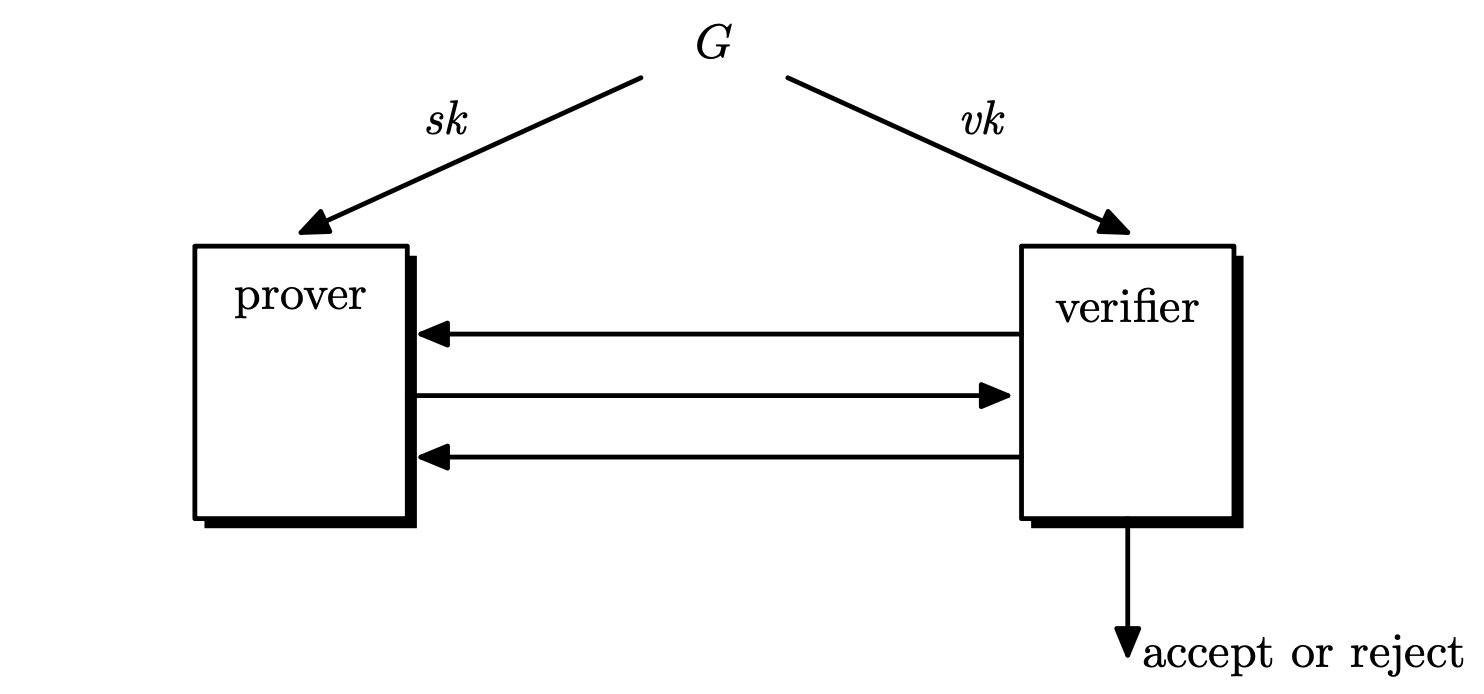
\includegraphics[width=0.6\linewidth]{figures/chapter18/fig1.png}
    \caption{身份认证协议中的证明者与验证者}
    \label{fig:18—1}
\end{figure}

\begin{definition}
一个\textbf{身份识别协议} $\mathcal{I}=(G,P,V)$ 由三部分组成:
\begin{itemize}
    \item $G$ 是一个概率性的\textbf{密钥生成}算法,不接受任何输入,并输出一对密钥 $(vk,sk)$,其中 $vk$ 被称为\textbf{验证密钥 (verification key)},$sk$ 被称为\textbf{私钥 (secret key)};
    \item $P$ 是一个交互式协议算法,被称为\textbf{证明者 (prover)},它接受 $sk$ 作为输入;
    \item $V$ 是一个交互式协议算法,被称为\textbf{验证者 (verifier)},它接受 $vk$ 作为输入,输出 $\mathsf{accept}$ 或 $\mathsf{reject}$。
\end{itemize}
我们要求,当 $P(sk)$ 和 $V(vk)$ 能够正确交互时,$V(vk)$ 总是输出 $\mathsf{accept}$。也就是说,对于 $G$ 的所有可能输出 $(vk,sk)$,如果 $P$ 由 $sk$ 初始化,$V$ 由 $vk$ 初始化,那么当 $P$ 和 $V$ 交互结束时,$V$ 输出 $\mathsf{accept}$ 的概率为 $1$。

\end{definition}
\section{口令协议:针对直接攻击的安全性}\label{sec:18-3}

在\textbf{基本口令协议 (Basic Password protocol)}中,证明者的密钥是一个\textbf{口令} $pw$。在该协议中,证明者将 $pw$ 发送给验证者,验证者需要检查 $pw$ 是否是合法的口令。因此,该协议的密钥 $sk$ 就是 $pw$。显然,只有当对手无法窃听证明者和验证者之间的交互时,这个协议才可以被使用。为了完善对基本口令协议的定义,我们还需要指定验证者如何检查给定的口令是否合法。

首先想到的方法是直接将验证者的公钥也定义为 $vk:=pw$,这样验证者只需要检查他从证明者那里收到的口令与 $vk$ 是否相等即可。但是这种简陋的协议显然是有问题的,因为如果验证者被攻破,所有验证者存储的口令都会直接泄露。

为了避免这个问题,我们可以让验证者保存口令的哈希值,而不是口令本身。我们称这个修改后的口令协议为\textbf{版本 1}。我们下面用一种相当理想化的方式来描述这个协议,在该协议中,我们从某个有限的口令空间中随机均匀地选择口令,但实际情况可能并非如此。

\begin{snote}[口令协议版本 1.]
证明者的私钥 $sk$ 是一个从有限口令空间 $\mathcal P$ 中随机均匀选出的口令 $pw$,验证者的公钥 $vk=H(pw)$,其中的哈希函数为 $H:\mathcal{P}\to\mathcal{Y}$。这样,\textbf{口令身份认证协议} $\mathcal{I}_{\rm pwd}=(G,P,V)$ 的定义如下:
\begin{itemize}
    \item $G$:令 $pw\xleftarrow{\rm R}\mathcal{P}$ 并输出 $sk=pw$ 和 $vk=H(pw)$。
    \item 以 $sk=pw$ 为输入的算法 $P$ 及以 $vk=H(pw)$ 为输入的算法 $V$,它们按照以下方式交互:
    \begin{enumerate}
        \item $P$ 将 $pw$ 发送给 $V$;
        \item 如果收到的 $pw$ 满足 $H(pw)=vk$,$V$ 输出 $\mathsf{accept}$,否则输出 $\mathsf{reject}$。
    \end{enumerate}
\end{itemize}

在一个多用户系统中,验证者(服务器)通常会在数据库中维护一张口令映射表,就像图 \ref{fig:18-2} 一样。因此,对服务器的攻击不会泄露出任何的明文口令。

为了分析上述口令协议的安全性,我们下面首先正式定义针对直接攻击的安全性,然后解释为什么上面的协议能够满足这个安全定义。
\end{snote}

\begin{figure}
    \centering
    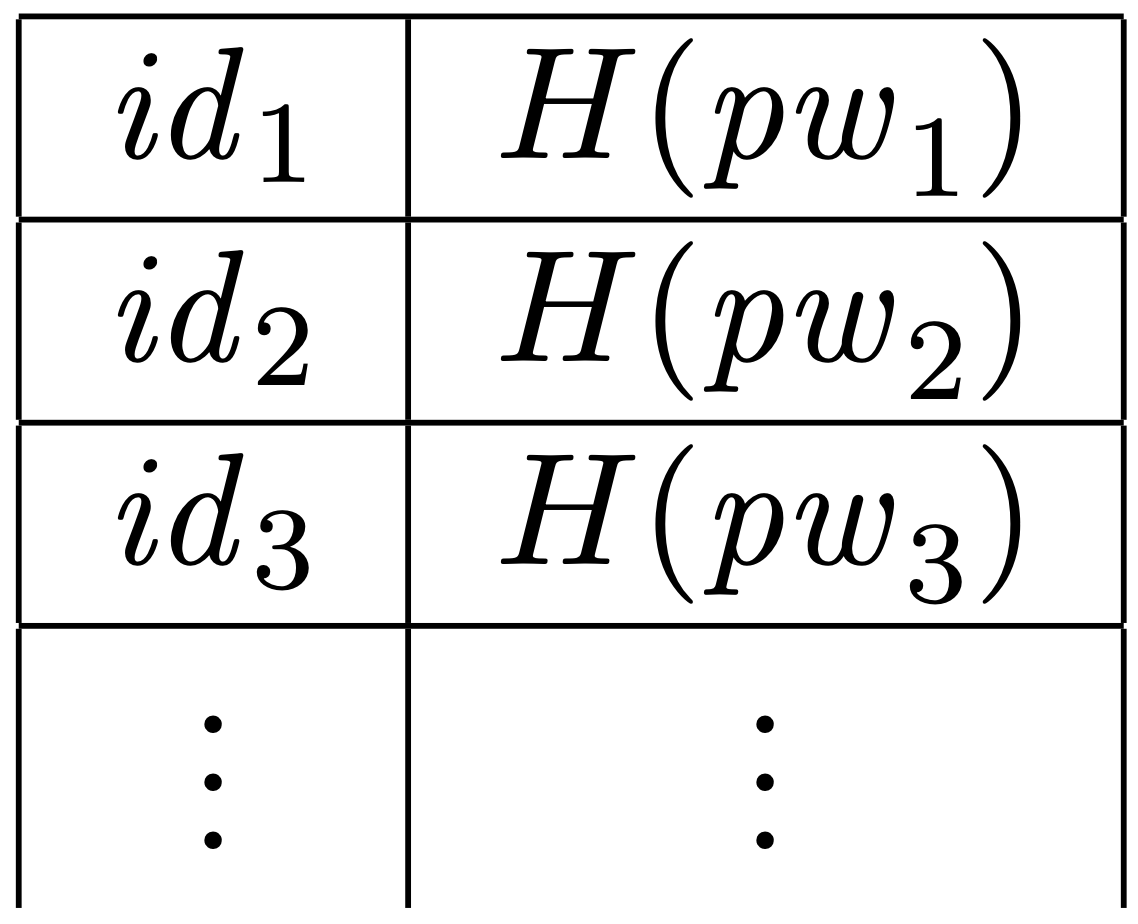
\includegraphics[width=0.17\linewidth]{figures/chapter18/fig2.png}
    \caption{储存在服务器中的口令文件(版本1)}
    \label{fig:18-2}
\end{figure}

\begin{game}[针对直接攻击安全的身份识别]\label{game:18-1}
对于一个给定的身份识别协议 $\mathcal{I}=(G,P,V)$ 和一个给定对手 $\mathcal{A}$,攻击游戏按照以下方式运行:
\begin{itemize}
    \item 密钥生成阶段。挑战者运行 $(vk,sk)\xleftarrow{\rm R} G()$ 并将 $vk$ 发送给 $\mathcal{A}$。
    \item 仿冒尝试阶段。挑战者与 $\mathcal{A}$ 交互,其中挑战者掌握 $vk$,并按照验证者的算法 $V$ 运行,而对手 $\mathcal{A}$ 扮演证明者的角色,但不一定会诚实执行证明者的算法 $P$(事实上 $\mathcal{A}$ 根本没有获取到私钥 $sk$)。
\end{itemize}
如果 $V$ 在交互结束时输出 $\mathsf{accept}$,我们就称对手 $\mathcal{A}$ 赢得了本游戏。我们定义 $\rm{ID1\mathsf{adv}}[\mathcal{A},\mathcal{I}]$ 为对手 $\mathcal{A}$ 相对 $\mathcal{I}$ 的优势,其值为 $\mathcal{A}$ 赢得本游戏的概率。{\hfill $\square$}
\end{game}

\begin{definition}\label{def:18-2}
如果对于任意有效对手 $\mathcal{A}$,$\rm{ID1\mathsf{adv}}[\mathcal{A},\mathcal{I}]$ 的值都可以忽略不计,我们就称身份识别协议 $\mathcal{I}$ \textbf{对于直接攻击是安全的}。
\end{definition}

请注意,在游戏 \ref{game:18-1} 中,对手 $\mathcal{A}$ 能够获得的是验证密钥 $vk$。因此,一个将明文口令直接存储的简陋口令协议并不满足定义 \ref{def:18-2}。下面的简单定理表明,版本1的协议是安全的。

\begin{theorem}\label{theo:18-1}
如果哈希函数 $H:\mathcal{P}\to\mathcal{Y}$ 是单向的,那么口令协议 $\mathcal{I}_{pwd}$ 针对直接攻击是安全的。
\end{theorem}

\begin{proof}[证明简述]
为了攻击协议 $\mathcal{I}_{pwd}$,对手 $\mathcal{A}$ 必须能够提供一个口令 $pw'$ 使得 $H(pw')=H(pw)$。需要注意的是 $pw'$ 可能与 $pw$ 不同。而能够提供满足上述要求的 $pw'$ 的对手显然已经破坏了 $H$ 的单向性。
\end{proof}

我们可以注意到,针对直接攻击(见攻击游戏 \ref{game:18-1})的安全性事实上是一个非常弱的安全概念。比如说,尽管口令协议 $\mathcal{I}_{pwd}$ 对于直接攻击是安全的,但是对手哪怕能够窃听到协议的一个实例,它显然就丧失了安全性。

\subsection{利用字典攻击破解口令}

口令协议 $\mathcal{I}_{pwd}$ 在实践中被广泛使用,因为它使用起来非常方便。任何人只要记住一个口令 $pw$,就可以参与到协议中来,扮演证明者的角色,并且不需要任何额外的计算设备。问题是,人类生成和记忆随机口令的能力是在太过糟糕。在实践中,被使用的口令通常太短了。更糟糕的是,口令通常根本就不是随机生成的,而是根据一些可预测的信息推导来的。

\begin{figure}
    \centering
    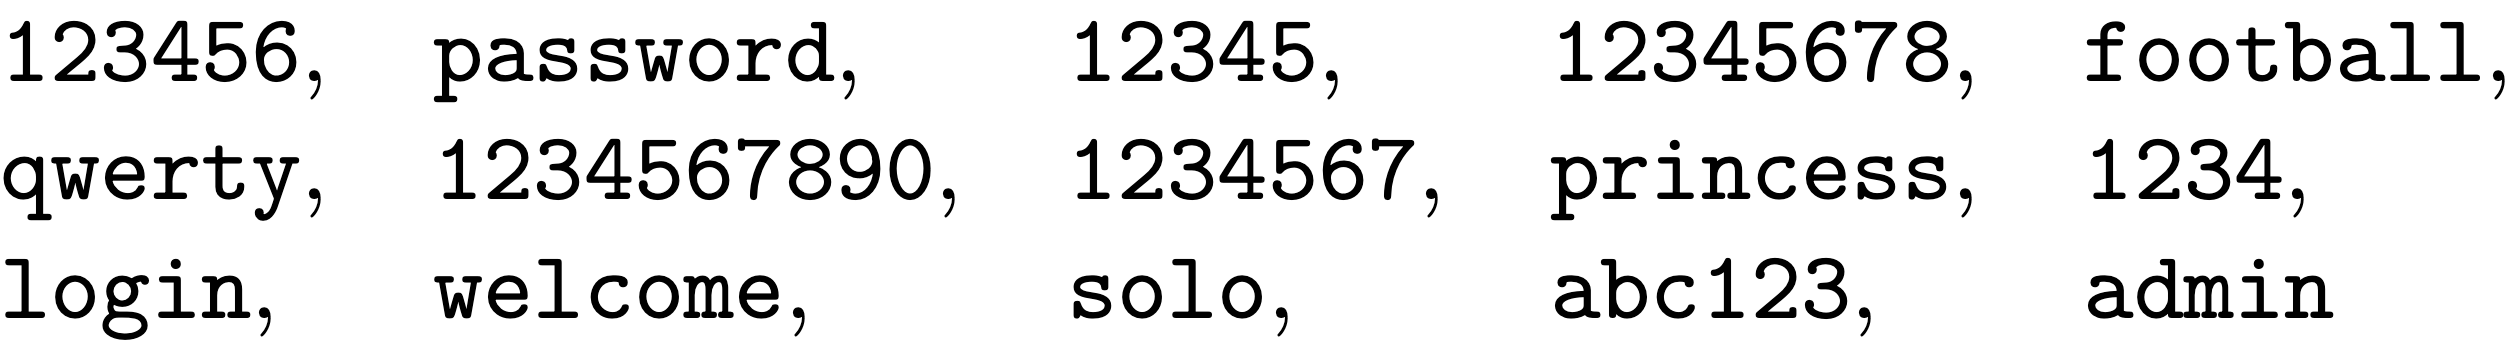
\includegraphics[width=0.6\linewidth]{figures/chapter18/fig3.png}
    \caption{依次列出的2016年中最常见的15个口令}
    \label{fig:18-3}
\end{figure}

图 \ref{fig:18-3} 总结了2016年进行的一项研究的结果,该研究检查了500万个泄露的口令,这些口令大多由北美和西欧的用户持有。数据显示,这些口令与大集合上的均匀分布相去甚远,尤其是有相当比例的口令属于相对较小的常用口令字典。大约4\%的人使用``123456"这个口令,而大约10\%的人使用前25个最常用口令列表中的某一个。图 \ref{fig:18-3} 中的口令列表在一段时间内非常稳定。每年的变化都非常小。

从现在开始,我们使用\textbf{强口令}来表示从一个很大口令空间 $\mathcal{P}$ 中随机均匀选出的口令。只有口令是强口令时,定理 \ref{theo:18-1} 的安全性声明才有效。相对地,\textbf{弱口令}就是指那些从一些常用口令的小字典中按照某个任意分布选取的口令。我们将弱口令的口令空间表示为 $\mathcal{D}$,则必然有 $\mathcal{D}\subseteq\mathcal{P}$。

\subsubsection{在线字典攻击}

假设现在有一个对手怀疑某个用户的口令很弱,属于某个常用口令的小字典 $\mathcal{D}$。那么对手就可以发动一个\textbf{在线字典攻击}:他只需要逐一尝试 $\mathcal{D}$ 中的所有口令,直到找到匹配的口令。为了进一步提升效率,对手可以按照流行程度对 $\mathcal{D}$ 中的元素进行排序,首先尝试更流行的口令。

一个常见的防御在线字典攻击的方法是,在特定用户 ID 或来自特定 IP 地址的登录尝试每两次失败后,就将服务器的响应时间增加一倍。因此在十次登录失败后,下一次尝试的时间就会是正常响应时间的 32 倍。即使一个用户并不能熟记自己的口令,他也不过需要等待一点时间,所以对他来说这种设计的影响并不大。但是对于恶意攻击者来说,通过暴力破解的方式去猜测口令会变得非常困难。

对手为了应对这种反制对策,可以在许多不同的用户名中尝试同一个普通的口令,比如 $\mathtt{123456}$。此外,对手可以利用位于不同 IP 地址的肉机来反制对于单个 IP 地址的登录尝试次数限制。用这种方式对随机账户进行攻击对于一般的对手来说往往已经足够了,他们通常会在地下论坛中交易攻击得到的数据。

非密码学的防御手段对于阻吓这些在线攻击已经很有效了。但是仍然有更具破坏性的攻击,这种攻击也更难阻止。我们将在接下来讨论这种攻击。

\subsubsection{离线词典攻击}\label{subsubsec:18-3-1-2}

攻击者如果破坏了登录服务器,就可以窃取存储在服务器上的口令数据库。这给了攻击者一个大的哈希口里ing列表,每个在该系统注册的用户都有一个口令。

侵入登录服务器的对手可以窃取服务器上存储的口令数据库,攻击者可以借此得到大量哈希后的口令。除了直接破坏服务器外,还有许多其他方法可以获得口令文件。例如一项研究表明,在eBay上购买的二手硬盘可以包含很多有趣的、未被删除的数据,其中就包括口令文件。

现在假设一个对手设法获得了某个用户的验证密钥 $vk=H(pw)$。如果口令 $pw$ 是弱的,并且属于某个常见口令的小字典 $\mathcal{D}$,那么对手就能够发动\textbf{离线字典攻击},他可以这么做:
\begin{equation}\label{eq:18-1}
	\begin{aligned}
		& \text{对每个~}w\in\mathcal{D}:\\
		& \text{~~~~~~~~如果~}H(w)=vk:\\
		& \text{~~~~~~~~~~~~~~~~输出~} w \text{ 并停机}
	\end{aligned}
\end{equation}
如果 $pw$ 在 $\mathcal{D}$ 中,那么依照上述过程,对手迟早能够获取 $pw$,抑或是另一个 $pw'$ 使得 $H(pw')=H(pw)$。

这种离线字典攻击的时间复杂度是 $O(|\mathcal{D}|)$,其中时间单位为对一个输入计算一次$H$的耗时。这种计算完全可以\emph{脱机}运行,不需要与证明者或服务器有任何交互。

\begin{snote}[口令统计.]
2016年,一个名为 CrackStation 的口令破解服务发布了一个大小约为 15 亿的的常用口令词典。经验证据表明,人类生成的口令中有接近 50\% 都在这个列表中。这意味着,每经过约 15 亿次的离线哈希,每两个口令中就有一个能被破解。如果哈希函数 $H$ 是 SHA256,那么现代 GPU 只需要不到一分钟的时间就能够完成破解。由此我们能够得出一个结论:简单地使用 SHA256 对口令进行哈希处理对保护口令数据来说远远不够。

从另一个角度来说,我们可以发现,只包含可打印字符的 8 位字符口令的总数大约是 $95^8 \approx 2^{52}$ 个,这是因为美式键盘上有 95 个可输入字符。使用现代 GPU 阵列对这组口令中的所有单词运行 SHA256 也不过仅仅几天就可以完成。这说明,\emph{所有}8位以下长度口令在服务器被攻破的情况下都是不安全的。
\end{snote}

\begin{snote}[量子离线口令攻击.]
更糟糕的是,一旦有了大规模的量子计算机,上面的穷举搜索攻击将会更加容易。我们在4.3.4节中介绍过,量子计算机可以在 $\sqrt{n}$ 级别的时间内搜索大小为 $n$ 的空间。因此对于 8 位长度的口令空间来说,量子搜索相当于只需要进行 $\sqrt{2^{52}}=2^{26}$ 次哈希计算。这在现代经典计算机上也仅仅需要几秒钟而已。换言之,由于 8 位长度口令在经典计算机上是不能抵抗穷举搜索的,所以一旦我们拥有一台在速度和大小上与当前经典计算机相当的量子计算机,16 位长度的口令也将失去安全保障。我们将在18.4.3节中讨论一些针对该问题防御措施。
\end{snote}

\subsubsection{含预处理的离线字典攻击}

如果对手能够在发动攻击之前对字典 $\mathcal{D}$ 进行预处理,那么上面讨论的离线字典攻击将会更容易发动。一旦获取了哈希后的口令 $vk$,对手就能够立即从字典中查到原始口令 $pw$。具体来说,我们可以将字典攻击分为两个阶段:一个\textbf{预处理阶段},在获取任何哈希口令之前发动;一个\textbf{攻击阶段},针对特定口令$vk$发起攻击。我们的目标是尽量减少攻击阶段破解特定 $vk$ 所需的时间。

一个简单的带有预处理阶段的字典攻击原理如下:
\begin{equation}\label{eq:18-2}
	\begin{aligned}
		& \text{预处理阶段}:\\
		& \text{~~~~~~~~对于每个~}pw\in\mathcal{D}\text{,将~}(pw,H(pw))\text{~加入列表~}L\\
		& \text{针对输入~}vk\text{~的攻击阶段}:\\
		& \text{~~~~~~~~如果在表~}L\text{~中存在一项~}(pw,vk)\text{,则输出~}pw\\
		& \text{~~~~~~~~否则输出~}\mathsf{fail}
	\end{aligned}
\end{equation}
假设我们把对一个口令计算一次$H$的耗时作为时间单位,那么预处理阶段所需要的时间为 $O(|\mathcal{D}|)$级。如果表 $L$ 存储在一个支持常数时间查找的哈希表中,那么攻击阶段将会非常快,耗时仅仅为常数级。

\begin{snote}[批量离线字典攻击.]
一旦完成预处理,攻击者就能利用它快速破解许多哈希口令。具体来说,假设攻击者从一个被攻破的登录服务器中获得了一个大型的哈希口令数据库 $F$,那么现在使用字典 $\mathcal{D}$ 破解 $F$ 中的哈希后口令仅需要:
\begin{equation}
	\begin{aligned}
		& \text{预处理阶段:}O(|\mathcal{D}|)\\
		& \text{攻击阶段:}O(|F|)
	\end{aligned}
\end{equation}
其中 $|F|$ 指 $F$ 中哈希口令的数量。上述批量离线字典攻击的总工作量是 $O(|\mathcal{D}|+|F|)$,这比针对 $F$ 中每一个元素分别单独发起式 \ref{eq:18-1} 的离线字典攻击要快得多,因为后者的总工作量是 $O(|\mathcal{D}|\times |F|)$。

回忆一下,\ref{subsubsec:18-3-1-2} 节中的统计数据表明,对手可以使用 CrackStation 字典找到 $F$ 中近\emph{半数}的口令。因此一旦完成预处理,只需要 $O(|F|)$ 时间就能完成攻击。事实上这种攻击能够使用极少的工作量暴露数百万个被破解的口令。
\end{snote}

\begin{snote}[时空权衡.]
式 \ref{eq:18-2} 所展示的基于预处理的字典攻击要求攻击者建立并存储一个包含大量哈希口令的列表 $L$。然而当字典 $\mathcal{D}$ 是所有 $2^{52}$ 个 8 字符口令的集合时,这个表 $L$ 可能会相当大,存储成本过高。在第18.7节中,我们会介绍一种名为\textbf{彩虹表}的方法,它在预处理阶段构建一个小得多的表$L$,并用它快速破解口令。比如说,在 $n:=|\mathcal{D}|$ 的情况下,该方法能够实现:
\begin{equation*}
	\begin{aligned}
		& \text{表大小:}O(n^{2/3})\\
		& \text{预处理时间:}O(n)\\
		& \text{攻击时间:}O(n^{2/3})
	\end{aligned}
\end{equation*}
表的大小从 $O(n)$ 缩减到 $O(n^{2/3})$ 级别。然而,攻击一个哈希口令的时间从 $O(1)$ 级增长到 $O(n^{2/3})$ 级。换言之,我们用更长的攻击时间换取了表 $L$ 大小的缩减。正因此,这种方法被称为\textbf{时空权衡}。我们通常不讨论预处理阶段的耗时,因为预处理是一个一次性过程,它在攻击开始之前就完成了。

这种时空权衡进一步说明了为什么简单地存储哈希口令是错误的做法。我们将在之后讨论针对性的防御措施。
\end{snote}
\section{使字典攻击更难实施}

当在服务器上存储弱口令的哈希时,离线字典攻击,尤其是基于预处理的离线字典攻击是一种真正的威胁。本节中,我们将讨论一些针对性的技术,这些技术能够使得字典攻击更加困难。

\subsection{公共盐}

上一节中,我们展示了攻击者如何对字典 $\mathcal{D}$ 进行预处理以构建一个速查表 $L$,进而可以快速破解一个或多个哈希后的口令。一种叫做\textbf{加盐(salting)}的简单防御措施就可以反制这种预处理攻击。就算允许攻击者拥有无限时间对 $\mathcal{D}$ 进行预处理,加盐也可以将破解一个哈希口令文件 $F$ 的时间复杂度提升到:
$$
\Omega(|\mathcal{D}|\times |F|)
$$
换言之,加盐可以确保没有任何其他方法的效率优于基于穷举搜索的暴力破解。

加盐的具体做法是在注册新口令时生成一个称为\textbf{盐(salt)}的随机字符串。系统中的每个用户都会被分配一个新的盐,我们可以认为盐是从一个集合 $\mathcal{S}$ 中随机选出的。在实践中,往往 $|\mathcal{S}|=2^{128}$ 就足以满足要求。这个盐会与口令一起被哈希,得到验证密钥 $vk$。盐也会被存储在服务器的口令表中,如图 \ref{fig:18-4} 所示。只有服务器需要知道盐值,用户甚至不需要知道有盐的存在。

\begin{figure}
  \centering
  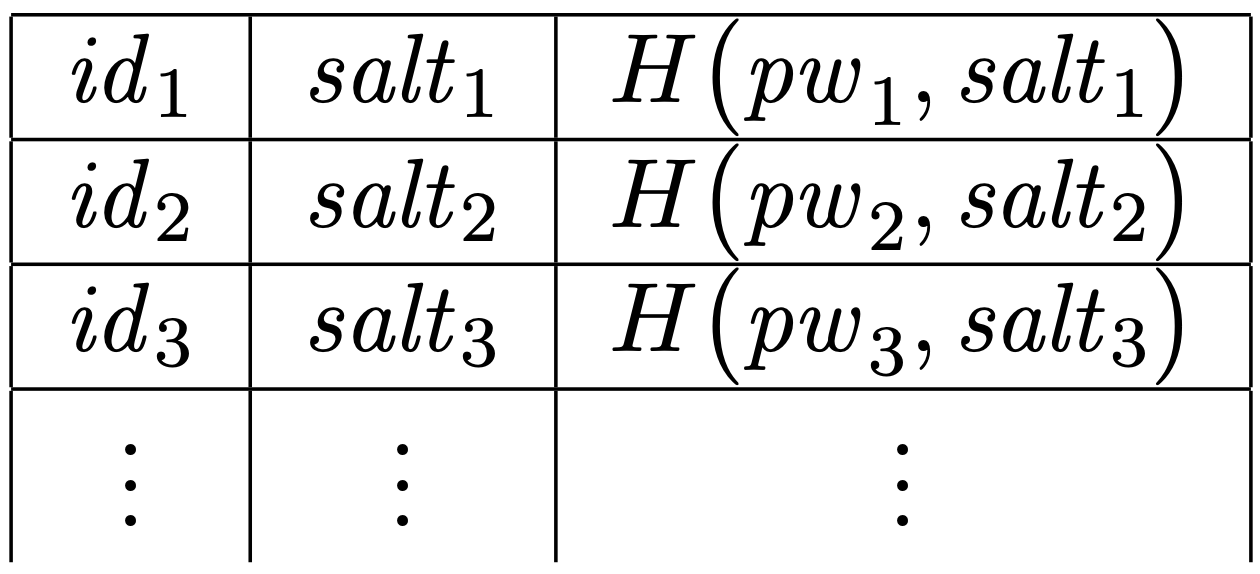
\includegraphics[width=0.3\linewidth]{figures/chapter18/fig4.png}
  \caption{口令文件(版本2)}
  \label{fig:18-4}
\end{figure}

于是我们就有了新的口令协议,我们称之为\textbf{口令协议版本2},它的运行方式如下:
\begin{itemize}
	\item $G$:令 $pw \xleftarrow{\rm R}\mathcal{P}$,$salt\overset{\rm R}\leftarrow\mathcal{S}$,计算 $y\leftarrow H(pw,salt)$,输出 $sk=pw$ 和 $vk=(salt,y)$。
	\item 以 $sk=pw$ 为输入的算法 $P$ 和以 $vk=(salt,y)$ 为输入的算法 $V$,按如下逻辑交互:
	\begin{enumerate}
		\item $P$ 将 $pw$ 发送给 $V$;
		\item 如果收到的 $pw$ 满足 $H(pw,salt)=y$,$V$ 输出 $\mathsf{accept}$,否则输出 $\mathsf{reject}$。
	\end{enumerate}
\end{itemize}
与版本 1 的描述一样,版本 2 的描述也是相当理想化的,因为我们假设口令 $pw$ 是从空间 $\mathcal{P}$ 中随机均匀选出的,但实际情况远非如此。

现在有了盐的存在,对手可以采取两种策略去攻击文件 $F$ 中的哈希口令:

\begin{itemize}
	\item 第一种策略是使用批量离线字典攻击。问题是,现在预处理阶段需要考虑哈希函数 $H$ 的庞大的输入集合,事实上集合 $\mathcal{D}\times\mathcal{S}$ 中的任何元素都是可能的输入。因此,如果仍然采用式 \ref{eq:18-2} 中的预处理算法,需要准备的预处理表 $L$ 的规模将达到 $|\mathcal{D}|\times|\mathcal{S}|$。这个大小无论如何都是难以生成的,更不要说出村了。因此,式 \ref{eq:18-2} 所介绍的预处理方法不再可行。
	\item 第二种策略是对 $F$ 中的所有口令进行穷举搜索,就像式 \ref{eq:18-1} 中所做的那样。我们已经说明过,穷举搜索的时间复杂度是
	$$O(|\mathcal{D}|\times |F|)$$
\end{itemize}

为了使得没有任何其他方法的效率优于穷举搜索,即上面的第二种策略,盐值空间 $\mathcal{S}$ 需要尽可能大。即使对手采用时空权衡的方法来对$\mathcal{D}\times\mathcal{S}$进行预处理,也同样应该成立。为了推导对 $\mathcal{S}$ 大小的必要约束,我们首先需要更精确地定义在预处理模型中逆转加盐函数的含义。

\begin{snote}[带有预处理的加盐单向函数.]
为了便于定义,我们将对手 $\mathcal{A}$ 拆分成两个独立的对手 $\mathcal{A}_0$ 和 $\mathcal{A}_1$,其中对手 $\mathcal{A}_0$ 拥有无限运行时间,执行预处理阶段。对手 $\mathcal{A}_1$ 能够高效地进行反转攻击。两个对手之间唯一允许的通信是交换一个 $\ell$ 比特的字符串 $L$,其中 $L$ 是预处理阶段的结果。这些概念在下面的定义中得到了体现,该定义将$H$建模为一个随机预言机。
\end{snote}

\begin{definition}\label{def:18-3}
	假设 $H$ 是一个定义在 $(\mathcal{D}\times\mathcal{S},\mathcal{Y})$ 上的哈希函数。我们定义对手 $\mathcal{A}=(\mathcal{A}_0,\mathcal{A}_1)$ 在预处理模型中攻破哈希函数 $H$ 的单向性的优势为 ${\rm OWsp^{ro}\mathsf{adv}}[\mathcal{A},H]$,其大小为对手 $\mathcal{A}$ 赢得下面游戏的概率:
	\begin{itemize}
		\item $\mathcal{A}_0$ 向 $H$ 发起查询并输出一个建议字符串 $L$;
		\item 挑战者随机选择 $(pw,s)\overset{\rm R}\leftarrow\mathcal{D}\times\mathcal{S}$,令 $y=H(pw,s)$,并将 $(L,y,s)$ 发送给 $\mathcal{A}_1$;
		\item $\mathcal{A}_1$ 向 $H$ 发起查询并输出 $pw'\in\mathcal{D}$。当 $H(pw',s)=y$ 时,$\mathcal{A}$ 获胜。
	\end{itemize}
\end{definition}

需要注意的是,对手 $\mathcal{A}_1$ 同时获得了 $L$ 和盐 $s$,而它的目的是找到带有盐 $s$ 的哈希 $y$ 的原象。下面的定理给出了在预处理模型中反转加盐单向函数 $H$ 的时间界限,其中 $H$ 符合随机预言机模型。

\begin{theorem}\label{theo:18-2}
	假设 $H$ 是一个定义在 $(\mathcal{D}\times\mathcal{S},\mathcal{Y})$ 上的哈希函数,$H$ 符合随机预言机模型,且 $|\mathcal{D}|\leq|\mathcal{Y}|$。令 $\mathcal{A}=(\mathcal{A}_0,\mathcal{A}_1)$ 是一个定义 \ref{def:18-3} 中的对手,其中 $\mathcal{A}_0$ 输出一个 $\ell$ 比特的建议字符串 $L$,$\mathcal{A}_1$ 最多能向 $H$ 发起 $Q_{\rm ro}$ 次查询,则有:
	\begin{equation}
	{\rm OWsp^{ro}\mathsf{adv}}[\mathcal{A},H]
	\leq
	O(\frac{\ell\cdot Q_{\rm ro}}{|\mathcal{S}|\cdot |\mathcal{D}|}+\frac{Q_{\rm ro}}{|\mathcal{D}|})	
	\end{equation}
\end{theorem}

该定理表明,如果 $\mathcal{A}$ 在反转 $vk:=y\in\mathcal{Y}$ 时有恒定成功概率,比如 $0.5$,那么它在攻击阶段必须至少花费 $Q_{\rm ro}\geq\Omega({|\mathcal{D}|\cdot|\mathcal{S}|}/{\ell})$ 的时长。因此,为了防止预处理带来的破解性能提升,我们应该令 $|\mathcal{S}|\geq\Omega(\ell)$,这会确保不会有其他方法效率优于穷举搜索。比如说,如果我们假设建议字符串 $L$ 的最大存储空间为 $2^{80}$,那么盐空间应当至少是 $\{0,1\}^{80}$。在实践中,人们通常取 $|\mathcal{S}|:=\{0,1\}^{128}$。

从技术上讲,定理 \ref{theo:18-2} 限定了破解\emph{单个}口令的时间,但并没有限定\emph{批量}离线字典攻击的时间。在这种情况下,攻击者可以尝试一次性破解 $t$ 个口令,其中$t>1$。然而,我们希望该定理可以被推广到批量攻击中,使得约束 $|\mathcal{S}|\geq\Omega(\ell)$ 即使面对批处理场景仍能够有效防止破解。

\begin{snote}[加盐的局限性.]
虽然加盐可以抵御预处理攻击,但它并不能阻止其他攻击。比如说,即使使用了盐,一个选择了弱口令的用户仍然容易受到式 \ref{eq:18-1}  中的那种离线字典攻击。在接下来的内容中,我们将展示如何对离线字典攻击提供进一步的保护。
\end{snote}

\subsection{秘密盐}

通过向人类口令中添加人工熵,我们可以使对手的破解变得更难。想法是从一个小空间 $\mathcal{S}_{\rm p}$ 中再随机挑选一个短字符串,称为\textbf{秘密盐 (secret salt)}或者\textbf{胡椒 (pepper)},并将其也纳入到哈希计算中。但是秘密盐\emph{不会}被记录在口令文件中,因此产生的口令文件如图 \ref{fig:18-5} 所示。

\begin{figure}
  \centering
  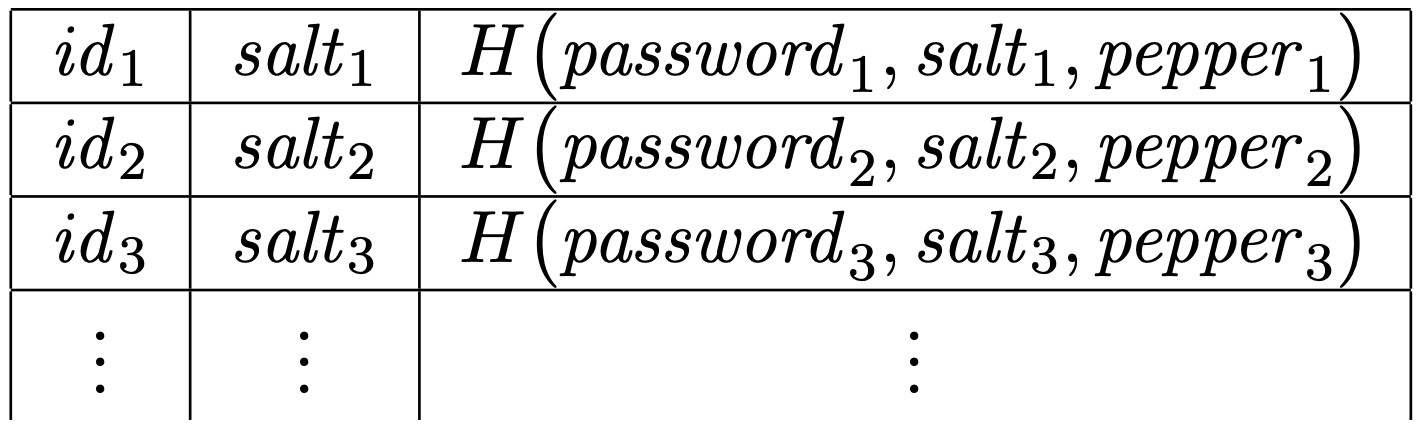
\includegraphics[width=0.45\linewidth]{figures/chapter18/fig5.png}
  \caption{口令文件(版本3)}
  \label{fig:18-5}
\end{figure}

为了验证一个口令,服务器只需要遍历秘密盐的所有可能值,直至找到一个能与存储的哈希值匹配的值。依此设计的\textbf{口令协议(版本 3)}按如下方式运行:
\begin{itemize}
	\item $G$:令 $pw\overset{\rm R}\leftarrow\mathcal{P}$,$salt\overset{\rm R}\leftarrow\mathcal{S}$,$pepper\overset{\rm R}\leftarrow\mathcal{S}_p$,$y\leftarrow H(pw,salt,pepper)$,输出 $sk:=pw$ 和 $vk:=(salt,y)$。
	\item 以 $sk=pw$ 为输入的算法 $P$ 及以 $vk=(salt,y)$ 为输入的算法 $V$,按如下逻辑交互:
	\begin{enumerate}
		\item $P$ 将 $pw$ 发送给 $V$;
		\item 对于收到的 $pw$,如果存在 $p\in\mathcal{S}_{\rm p}$ 满足 $H(pw,salt,p)=y$,$V$ 输出 $\mathsf{accept}$,否则输出 $\mathsf{reject}$。
	\end{enumerate}
\end{itemize}

一个典型的设计是将秘密盐空间设置为 $\mathcal{S}_{\rm p}:=\{0,1\}^{12}$。与版本 2 协议相比,这会使得服务器上的口令验证时长变为原来的 $4096$ 倍,但这在现代计算机上仍然只需要不到百分之一秒的时间,因此用户无法察觉到。然而更重要的是,对手现在破解口令文件中的弱口令的难度也增长到了原来的 $4096$ 倍。

秘密盐使离线字典攻击更加困难,因为现在对手必须在 $\mathcal{D}×\mathcal{S}_{\rm p}$ 空间中搜索,而不仅仅是 $\mathcal{D}$。这种技术对用户体验的影响很小。秘密盐增加了用户口令的熵,但并没有迫使用户记住更复杂的口令。

\subsection{慢哈希函数}

保护弱口令的另一种方法是使用慢哈希函数。回顾一下,用 SHA256 这样的哈希函数对口令进行哈希是非常快的,因此 SHA256 也使得离线字典攻击可能发动成功。现在假设服务器使用一个更慢的哈希函数对口令进行哈希,比如该函数处理一个输入需要百分之一秒,这比 SHA256 慢一万倍左右。尽管这对用户体验的影响微乎其微,但是对手这时再想要对字典中的所有项进行哈希的工作量就增大了一万倍。

那么我们如何构造一个慢哈希函数呢?一个直观的方法就是把一个快速哈希函数迭代足够多的次数,直至它变得很慢。具体地,对于一个定义在 $(\mathcal{X},\mathcal{X})$ 上的哈希函数 $H$,我们现在定义:
\begin{equation}\label{eq:18-5}
	H^{(d)}(x)=H(H(H(\cdots(x)\cdots)))
\end{equation}
这样就将 $H$ 迭代了 $d$ 次,可参见第 14.3 节。如果 $d=10000$,那么计算 $H^{(d)}(x)$ 就比计算 $H(x)$ 要多花一万倍的时间。然而这种方法是有问题的,它也不应该被应用到现实的系统中去。原因之一是,函数 $H^{(d)}(x)$ 也比函数 $H(x)$ 容易逆运算 $d$ 倍,参见练习 14.17。我们下面会介绍一个性质更好的函数。首先,我们先对慢哈希函数进行严格的定义。

\begin{definition}
	一个\textbf{基于口令的密钥推导函数(password-based key derivation function, PBKDF)}是这样的一个函数 $H$,其输入是一个口令 $pw\in\mathcal{P}$,一个空间 $\mathcal{S}$ 中的盐,以及一个难度参数 $d\in\mathbb{Z}^{>0}$;其输出是一个值 $y\in\mathcal{Y}$。我们要求函数 $H$ 能由一个运行时间与 $d$ 成正比的算法有效计算。像往常一样,我们称 PBKDF 定义在 $(\mathcal{P},\mathcal{S},\mathcal{Y})$ 上。
\end{definition}

我们会在练习 18.3 中讨论 PBKDF 的安全要求。我们的第一个 PBKDF 的例子,不妨称之为 \textbf{PBKDF1},就基于式 \ref{eq:18-5},其定义为:
$$
{\rm PBKDF1}_H(pw,salt,d)=H^{(d)}(pw,salt)
$$
对于定义在 $(\mathcal{X},\mathcal{X})$ 上的哈希函数 $H$,PBKDF1 定义在 $(\mathcal{P},\mathcal{S},\mathcal{X})$ 上,其中 $\mathcal{X}=\mathcal{P}\times\mathcal{S}$。由于存在练习 14.17 中所介绍的攻击方式,该构造不会被应用在实际的系统中。

\subsubsection{PBKDF2 函数}

一种在实践中被广泛用于构造慢哈希函数的方法被称为PBKDF2。令 $F$ 是一个定义在 $(\mathcal{P},\mathcal{X},\mathcal{X})$ 上的PRF,其中 $\mathcal{X}:=\{0,1\}^n$,那么由之派生出的 PBKDF,不妨用 $\text{PBKDF2}_F$ 表示,它也定义在$(\mathcal{P},\mathcal{X},\mathcal{X})$ 上,并按如下方式工作:
\begin{equation}\label{eq:18-6}
	{\rm PBKDF2}_F(pw,salt,d):=
	\left\{
	\begin{aligned}
		& x_0\leftarrow F(pw, salt)\\
		& \text{for }i=1,\dots,d-1:\\
		& ~~~~~~x_i\leftarrow F(pw,x_{i-1})\\
		& \text{output }y\leftarrow x_0 \oplus x_1 \oplus \cdots \oplus x_{d-1}\in\mathcal{X}
	\end{aligned}
	\right\}
\end{equation}
上面的式 \ref{eq:18-6} 描述了基本版的 PBKDF2,如果需要输出更多比特,对其稍加调整即可。事实上,PBKDF2 能够输出 $\mathcal{X}^b$ 中的一个元素,其中 $1<b<2^{32}$,方法是计算:
\begin{equation}\label{eq:18-7}
{\rm PBKDF2}_F^{(b)}(pw,salt,d):=
\left(
{\rm PBKDF2}_F(pw,salt_1,d),\dots,
{\rm PBKDF2}_F(pw,salt_b,d)
\right)
\in\mathcal{X}^b
\end{equation}
其中所有的$b$个盐都是由最初给定的盐派生而来的,方法是令$salt_i\leftarrow salt\,||\,{\rm bin}(i)$。这里的${\rm bin}(i)$是$i\in\{1,\dots,b\}$的32位二进制字符串表示。

在实践中,PBKDF2 通常使用 HMAC-SHA256 作为底层 PRF。难度 $d$ 的设置取决于项目需求和硬件速度。例如,iOS 10 中的备份钥匙包使用 PBKDF2 来保护,其中 $d$ 的值是一千万。在Windows 10 中,数据保护 API 默认使用 $d = 8000$,但使用 HMAC-SHA512 作为 PRF。

我们会在练习18.2和18.3中更详细地讨论PBKDF2的安全性。

\subsection{慢内存困难哈希函数}

PBKDF2 的一个重要问题是它容易受到并行硬件攻击。我们知道,大部分现代处理器都是基于缓存的,而计算单元只占整个处理器面积的一小部分。因此,一个商用处理器不能对许多输入进行并行 PBKDF2 计算,也不太适合进行离线字典攻击。

更有经验的攻击者通常会在支持高度并行的专用硬件上运行离线字典攻击,比如 GPU,FPGA,甚至是定制芯片。一个定制芯片可以包装超过一百万个 SHA256 计算单元。如果每个单元每秒可以进行一百万次 SHA256 计算,那么一个对手每秒可以在每个芯片上尝试 $10^{12}$ 个口令。即使 PBKDF2 的难度被设置为 $d=10000$,一个由大约 500 个这样的专用芯片组成的农场也能在不到一天的时间内跑完所有 $2^{52}$ 个 8 位口令。这种攻击之所以能够实现,是因为 SHA256 的硬件实现可以做得相当紧凑,所以大量的 SHA256 计算单元可以打包到一个芯片里。

这表明,我们需要的哈希函数 $H$ 应该要求专用硬件实现也需要庞大的片上面积,这样一个芯片就只能容纳几个计算单元,这就极大程度上降低了定制硬件的性能优势。

那么我们如何建立一个具有较大硬件占用面积的哈希函数 $H$?一种方法是确保计算 $H$ 的每一步都需要大量的内存,这将迫使攻击者将芯片上的大部分区域分配给单次哈希求值所需的内存,这就确保了每个芯片只能包含少量的计算电路。

需要大量内存的哈希函数被称为\textbf{内存困难函数}。已经有一些符合要求的内存难度哈希函数,这些函数能够在随机预言机模型下被严格证明是内存困难的。在我们讨论安全问题之前,让我们先看看一个流行的结构,叫做\textbf{Scrypt}。Scrypt是由一个内存容易的哈希函数$h:\mathcal{X}\rightarrow\mathcal{X}$,其中$\mathcal{X}:=\{0,1\}^n$。得到的函数记作$\text{Scrypt}_h$,如图 \ref{fig:18-6} 所示。

\begin{figure}
  \centering
  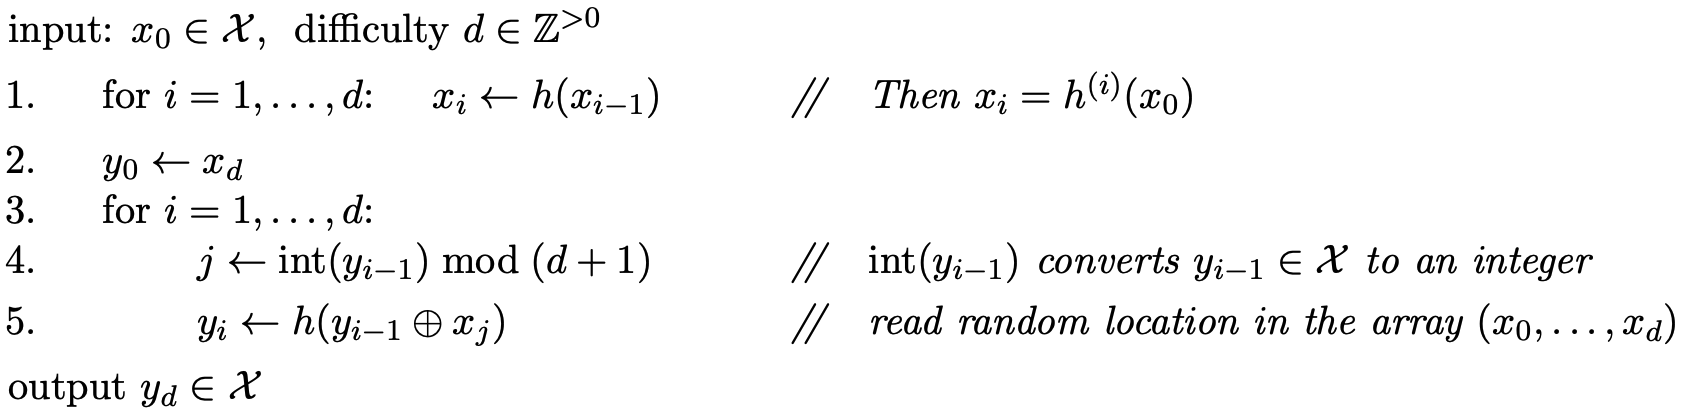
\includegraphics[width=0.85\linewidth]{figures/chapter18/fig6.png}
  \caption{函数$\text{Scrypt}_h(x_0,d)$}
  \label{fig:18-6}
\end{figure}

在我们的安全分析中,我们将底层哈希函数 $h$ 当作一个随机预言机。在实践中,函数 $h$ 是由 Salsa 20/8 变换衍生出来的,参见3.6节。难度 $d$ 是根据系统的性能需求来设置的。例如我们可以设置一个恰当的 $d$ 使得计算 Scrypt 需要填满整个芯片的存储空间。这会确保计算 Scrypt 不会太慢,但需要大量的内存。

图 \ref{fig:18-6} 是将Scrypt作为一个哈希函数的描述。另一方面,定义在 $(\mathcal{P},\mathcal{X},\mathcal{X})$ 上的Scrypt PBKDF是基于Scrypt哈希构建的,其工作原理如下:
\begin{equation}\label{eq:18-8}
	{\rm ScryptPBKDF}_h(pw,salt,d):=
	\left\{
	\begin{aligned}
		& x_0\leftarrow {\rm PBKDF2}_F(pw,salt,1)\\
		& y\leftarrow \text{Scrypt}_h(x_0,d)\\
		& \text{output }{\rm PBKDF2}_F(pw,y,1)
	\end{aligned}
	\right\}
\end{equation}
其中 $F$ 是一个定义在 $(\mathcal{P},\mathcal{X},\mathcal{X})$ 上的 PRF。在实践中,我们通常使用HMAC-SHA256作为$F$。如有需要,我们也可多次迭代 Scrypt,以使其速度更慢而不增加所需的内存。同样地,通过调整最后一行的PBKDF2的应用,它可以在$b>1$时输出$\mathcal{X}^b$中的一个元素,就像式 \ref{eq:18-7} 那样。

\begin{snote}[Scrypt 是内存困难的吗?]
通过存储 $\mathcal{X}$ 中的 $d+1$ 个元素,Scrypt 函数可以在 $O(d)$ 时间内被计算。Scrypt 哈希的构建步骤创建了一个大小为 $d+1$ 的数组 $(x_0,\dots,x_d)$,随后重复地从该数组中的随机位置读取数据。正因此,一个想要在 $O(d)$ 时间内完成计算的算法必须在内存中保存整个数组 $(x_0,\dots,x_d)$。但这个结论尚需严格证明。

危险的是,时空权衡可能使攻击者尝试牺牲更多的攻击时间来换取更少的内存消耗。这将是毁灭性的,因为减少的内存将允许攻击者将许多 Scrypt 计算单元打包到一个芯片中,而这正是我们想要极力避免的。

在练习18.6中,我们设计了一种针对Scrypt的简单的时空权衡。它表明对于任意的$1<\alpha<d/2$,只需要存储$\lceil d/\alpha\rceil$ 个$\mathcal{X}$中的元素,就可以在$O(\alpha d)$的时间内完成对 Scrypt 的计算。特别地,使用\emph{恒定}空间的Scrypt可以在$O(d^2)$时间内完成计算。然而这种类型的时空权衡并不能帮助对手。对手需要将$\alpha$倍的Scrypt计算单元装入一个芯片中,但每个计算单元的工作难度也变为原来的$\alpha$倍。因此与图 \ref{fig:18-6} 中的Scrypt实现相比,单个芯片的整体吞吐量并没有变化。尽管如此,我们仍然需要证明没有比Scrypt更好的时空权衡方案。

流水线是对内存难度的另一个威胁。假设存在一个算法,它在计算 Scrypt 时仅仅在算法的其中几个步骤中需要使用 $O(d)$ 的内存。如果算法在其余步骤中仅需要使用常数级的内存空间,那么攻击者就可以通过构建流水线来排列多个 Scrypt 计算单元,这些计算单元之间共享一个 $O(d)$ 大小的存储。这样,每个计算单元仅在它需要 $O(d)$ 存储的几个步骤中调用内存,在其他时间可以把存储释放给其他计算单元使用。这样一来,攻击者仍然可以把许多计算单元打包到一个芯片中,只需要共享一个 $O(d)$ 大小的存储阵列即可。为了防止这种形式的流水线,我们还需要证明每一个 Scrypt 实现都需要\emph{在许多计算步骤中}使用到 $O(d)$ 级别的内存。
\end{snote}

\begin{snote}[Scrypt 是内存困难的.]
为了证明 Scrypt 是内存困难的,我们首先需要定义一个安全模型来分析上面讨论的几种障碍。我们下面定义了一个抽象的并行随机预言机模型,其中的算法 $\mathcal{A}$ 能够并行查询多个输入在随机预言机 $h:\mathcal{Y}\to\mathcal{Z}$ 上的输出。

一个\textbf{并行随机预言机算法} $\mathcal{A}$ 将一个 $x\in\mathcal{X}$ 作为输入,并进行一系列的状态转换。在每个状态下,算法 $\mathcal{A}$ 都会向随机预言机 $h$ 发出一组查询,算法在收到查询的所有响应后就会转入下一状态。该过程将不断重复,直至算法终止,此时算法到达最终状态,其中包含算法的输出。所有中间状态都需要被记录,以便跟踪中间状态的大小。

形式上说,算法 $\mathcal{A}$ 实现了一个确定性映射:
$$\mathcal{A}:\mathcal{X}\times\mathcal{S}\times\mathcal{Z}^{\leq p}\to\mathcal{S}\times\mathcal{Y}^{\leq p}$$
其中 $p$ 是正整数,其工作流程如下:
\begin{itemize}
	\item $\mathcal{A}$ 被作为 $\mathcal{A}(x,\varepsilon,\varepsilon)$ 调用,它输出一个 $\mathcal{S}\times\mathcal{Y}^{\leq p}$ 中的元组 $(s_1,\overline y_1)$。这里,$s_1$ 是 $\mathcal{A}$ 的当前状态,$\overline y_1=(y_1,\dots,y_r)$ 是它对随机预言机 $h:\mathcal{Y}\to\mathcal{Z}$ 所发出的第一组并行查询。
	\item 对于 $i=1,\dots,t$,当 $\mathcal{A}$ 输出 $(s_i,\overline y_i)$,$\overline y_1=(y_1,\dots,y_r)\in\mathcal{Y}^{\leq p}$ 时,我们进行如下操作:
	\begin{itemize}
	  \item 并行地调用随机预言机 $h$,计算$\overline z_i\leftarrow (h(y_1),\dots,h(y_r))$,并且
	  \item 重新调用 $\mathcal{A}$ 并计算 $(s_{i+1},\overline y_{i+1})\leftarrow \mathcal{A}(x,s_i,\overline z_i)$。
	\end{itemize}
	\item 最终 $\mathcal{A}$ 输出 $(s,\varepsilon)$,这表示算法终止,输出值为 $s$。
\end{itemize}

算法 $\mathcal{A}$ 在输入 $x\in\mathcal{X}$ 上的运行时间就是 $\mathcal{A}$ 在终止之前被调用的总次数。以这种方式衡量运行时间,我们可以捕捉到一个事实,即硬件实现可以在多点上并行地计算哈希函数$h$。

我们现在记第 $i$ 步输入 $\mathcal{A}$ 的数据为 $st_i:=(s_i,\overline y_i)$,并称 $st_i$ 为 $i$ 时刻的输入状态。对于 $s\in\mathcal{S}$,我们令 $|s|$ 表示 $s$ 的比特位数,类似地,我们令 $|z|$ 表示 $z\in\mathcal{Z}$ 的长度。对于 $\overline z=(z_1,\dots,z_r)\in\mathcal{Z}^{\leq p}$,我们令 $|\overline z|:=\sum_{j=1}^r|z_i|$。那么当 $\mathcal{Z}=\{0,1\}^n$ 时,我们有 $|\overline z|=rn$。最后,我们将输入状态 $st=(s,\overline z)$ 的长度定义为 $|st|:=|s|+|\overline z|$。
\end{snote}

\begin{definition}
	令 $\mathcal{A}$ 是一个以 $\mathcal{X}$ 中元素作为输入的并行随机预言机算法。记$\mathcal{A}$ 对于随机预言机 $h:\mathcal{Y}\to\mathcal{Z}$ 和 $x\in\mathcal{X}$ 的累计存储复杂度为 ${\rm mem}[\mathcal{A},h,x]$,其定义是:
	$${\rm mem}[\mathcal{A},h,x]:=\sum_{i=1}^t|st_i|$$
\end{definition}

图 \ref{fig:18-6} 中对于预言机$h:\mathcal{X}\to\mathcal{X}$,$\mathcal{X}=\{0,1\}^n$计算$\text{Scrypt}_h(x,d)$的算法的累计存储复杂度是$O(nd^2)$。下面的定理将表示,这种设计是最优的。

\begin{theorem}\label{theo:18-3}
	令 $\mathcal{X}=\{0,1\}^n$ 是一个满足 $|\mathcal{X}|$ 为超多项式的空间,$d$ 为一个使得 $2^{-d}$ 可以忽略不计的值。对于所有的并行随机预言机算法 $\mathcal{A}$ 和所有的 $x\in\mathcal{X}$,都有:
	$$
	  {\rm Pr}
	  \left[
	    \mathcal{A}(x,d)={\rm Scrypt}_h(x,d)
	  \right]
      \leq
      {\rm Pr}
      \left[
      {\rm mem}[\mathcal{A},h,(x,d)]\geq\Omega(d^2n)
      \right]+\delta
    $$
    其中 $\delta$ 是一个可以忽略的值。上面的两个概率都基于随机预言机 $h:\mathcal{X}\to\mathcal{X}$的选择。
\end{theorem}

该定理表明,如果 $\mathcal{A}(x,d)$ 以接近 $1$ 的概率输出 ${\rm Scrypt}_h(x,d)$,那么对于几乎所有的 $h$ 的选择,$\mathcal{A}$ 的累计存储复杂度一定是 $\Omega(d^2n)$ 级的。这表明不可能存在一个针对 Scrypt 的时空权衡策略使得其表现比练习18.6更好。如果一个算法以最大 ${dn}/{\alpha}$ 的存储空间计算 Scrypt,其中 $\alpha>1$,那么它的运行时间必然是 $\Omega(d\alpha)$。否则其累计存储复杂度将突破下限。

同样地,不可能存在对 Scrypt 的流水线式攻击。任何在 $O(d)$ 时间内运行的计算 Scrypt 的可行算法必须在整个算法中使用 $\Omega(d\alpha)$ 的内存。否则其累计存储复杂度也将突破下限。

从技术上讲,定理 \ref{theo:18-3} 限定了在\emph{单一}输入下计算Scrypt所需的时间和空间。它并没有限定\emph{批量}离线字典攻击的时间,此时攻击者试图一次对$p>1$个口令计算Scrypt。然而,我们期望该定理可以被推广到批量的设置中:如果一个算法$\mathcal{A}$对$p$个输入正确地计算了Scrypt的概率接近$1$,那么$\mathcal{A}$的累计存储复杂度一定是$\Omega(d^2np)$。这将表明,在$p$个点上计算Scrypt时,不存在针对Scrypt的时空权衡或流水线攻击。

\subsubsection{模糊口令内存困难函数}

虽然Scrypt是一个健全的内存困难的口令哈希函数,但它很容易受到第4.3.2节中讨论的那种侧信道道攻击。

考虑一个登录服务器,其中一个运行中的进程 $P$ 通过 Scrypt 哈希并验证用户的口令。假设对手获得了对该服务器的低权限访问,对手可以在服务器上运行用户级程序但不能破坏进程 $P$,也不能观察到用户的口令明文。然而,利用这种权限,它仍然可以发起一个名为\textbf{缓存计时攻击 (cache timing attack)} 的巧妙攻击方法,这种攻击能够让攻击者了解到 $P$ 访问内存页的顺序。注意,攻击者并不能知道内存页中存储的内容,它只能获取 $P$ 读取页的顺序。

现在,假设对手捕获了一个哈希值 $y$,它是将式 \ref{eq:18-8} 中介绍的Scrypt PBKDF应用于某个带有公共盐的口令 $pw$ 的结果。通常情况下,对手需要发起一个字典攻击,每次尝试都需要大量的时间和\emph{内存}。然而如果对手掌握了进程 $P$ 在计算$pw$的Scrypt哈希时的的内存访问模式,它就可以用很少的内存对 $pw$ 进行字典攻击。

为了说明如何实现攻击,让我们回顾一下图 \ref{fig:18-6} 中所介绍的Scrypt 的实现。算法在第一次执行第 5 步时,需要从数组$(x_0,\dots,x_d)$读取$j$号元素,其中$j={\rm int}(y_0)\mod(d+1)$。

通过观察 $P$ 对内存的访问,对手可以看到算法第一次执行第5步时读取了哪一页的内存,这就给了对手一个 $j$ 的近似值 $j_a$。由于一个内存页中可能存储了多个数组单元,所以对手并没有办法获取 $j$ 的精确值。尽管如此,这个 $j_a$ 也足以使用有限的内存来测试一个可能的口令$pw'$,方法是:
\begin{enumerate}
	\item 按式 \ref{eq:18-8} 计算 $x_0'\leftarrow{\rm PBKDF2}_F(pw',salt,1)$,
	\item 如图 \ref{fig:18-6} 那样计算 $y_0'$,但不存储任何中间值,然后
	\item 测试 $j'\leftarrow{\rm int}(y_0')\mod(d+1)$ 是否与 $j_a$ 接近。
\end{enumerate}

如果测试失败,那么 $pw'$ 就不是正确的口令。这个过程让对手用很少的内存就能过滤掉字典中的大部分候选口令。这样,用户的口令又变得容易受到硬件攻击。

\begin{snote}[一个解决方案.]
这种攻击之所以有效,是因为 Scrypt 的内存访问模式取决于用户的口令。如果我们有一个可证明安全的内存困难哈希函数,其内存访问模式与用户的口令无关,那就更好了。它仍然可以依赖于用户的盐,因为盐不是秘密。这样的函数被称为\textbf{数据模糊内存难度函数}。这种函数的一个例子是 \textbf{Argon2i B},它与 Scrypt 密切相关,但其第一部分的内存访问模式与口令无关,这就消解了上面描述的侧信道攻击。
\end{snote}

\begin{snote}[慢哈希与秘密盐.]
总结本小节,我们观察到秘密盐方法和慢哈希方法都会增加对手的工作负荷。人们可以使用其中的一种方法,但不能两者兼用。慢速内存难度哈希方法的主要好处是,它使定制的硬件攻击难以实施。与快速哈希函数一起使用的秘密盐并不能防止并行硬件攻击,因此慢内存困难哈希比秘密盐更可取。
\end{snote}

\subsection{其他口令管理问题}

\begin{snote}[共同口令问题 (common password problem).]
用户经常在多台机器和多个网站上拥有账户。理想情况下,所有这些服务器都会采取适当的预防措施来防止对手获得口令文件,并对口令进行适当的加盐和哈希,以降低对手获得该文件时的损失。不幸的是,低安全性服务器的设计者可能不会采取与高安全性服务器一样的安全预防措施。这种低安全性的服务器可能更容易被入侵。此外,这种低安全性的服务器可能会存储没有盐的口令哈希,这使批量字典攻击成为可能,并将检索出所有的弱口令。更糟糕的是,有些服务器甚至会在明处存储哈希值,这样对手就会检索出所有的口令,甚至是强口令。因此对手可以侵入一个低安全级别的服务器,并在该服务器上检索到一些,甚至所有的用户 ID/口令,而且这些口令中的一些也很有可能被用在高安全级别的服务中。因此,尽管在高安全性的服务器上采取了所有的预防措施,但该服务器的安全性可能会被一些完全不相关的、低安全性的服务器的不良安全性所破坏。这个问题被称为\textbf{共同口令问题}。

解决共同口令问题的一个标准方案是安装客户端软件,它能将通用口令转换为独有的网站口令,也就是个 "客户端盐"。令 $H$ 是一个哈希函数,如果用户名为 $id$ 的用户的口令是 $pw$,这个口令将在登录时发送给服务器 $id_{\rm server}$。用户的客户端或浏览器在发送前会将口令 $pw$ 转换为 $\widehat{pw}:=H(pw,id,id_{\rm server})$,然后将 $\widehat{pw}$ 发送给服务器。这样,从服务器的角度来看,用户的口令是 $\widehat{pw}$,而从用户的角度来看,口令仍然是 $pw$。这种技术可以保证,即使该用户在许多服务器上使用同一个口令,也不会受到那些没有正确加盐和哈希的服务器的影响。
\end{snote}

\begin{snote}[生物识别技术 (biometrics).]
基于口令的认证的最大困难是用户往往会忘记他们的口令。所有支持电话中的很大一部分都与口令相关的问题有关。因此,一些已部署的系统试图用人类生物识别技术来取代口令,如指纹、视网膜扫描、面容识别和许多其他技术。人们甚至可以使用击键动态,即击键之间的时间长度和按下一个键的时长作为一种生物识别特征。这个想法是使用生物特征作为用户的口令。

虽然生物识别技术相比口令而言有明显的好处,例如用户不会忘记他们的指纹,但它有两个明显的缺点:
\begin{itemize}
	\item 生物识别技术通常不是机密的,人们会在他们接触的几乎任何东西上留下他们的指纹;
	\item 生物识别技术是不可逆的,一旦生物识别特征被盗,用户就无法追索。
\end{itemize}
因此,生物识别技术不应该被用作识别用户的唯一手段,只适合作为额外的识别手段(有时被称为第二因素认证)来提高安全性。
\end{snote}
\section{一次性口令:针对窃听的安全性}\label{sec:18-5}

如果对手能够窃听证明者和验证者之间的单独某一次交互,上一节中的口令协议就很容易被破坏。在这一节中,我们的目标是开发防窃听的身份识别协议。首先,我们需要定义存在窃听者的情况下的 ID 协议安全性。我们通过引入一个新的``窃听阶段"来加强攻击游戏 \ref{game:18-1}。在该阶段中,对手可以要求获取真正的证明者和真正的验证者之间的一些交互记录。更新后的攻击游戏如图 \ref{fig:18-7} 所示。

\begin{figure}
  \centering
  \input{figures/chapter18/fig7.tex}
  \caption{攻击游戏 \ref{game:18-2}}
  \label{fig:18-7}
\end{figure}

\begin{game}[安全的身份识别:窃听攻击]\label{game:18-2}
对于一个给定的身份识别协议 $\mathcal{I}=(G,P,V)$ 和一个给定的对手 $\mathcal{A}$,攻击游戏运行如下:
\begin{itemize}
	\item \emph{密钥生成阶段。}挑战者运行 $(vk,sk)\overset{\rm R}\leftarrow G()$,然后将 $vk$ 发送给对手 $\mathcal{A}$。
	\item \emph{窃听阶段。}对手请求若干条(比如 $Q$ 条)$P$ 与 $V$ 之间交互的记录。挑战者会运行 $Q$ 次 $P$ 与 $V$ 的交互,在其中的每一次中,$P$ 都以输入 $sk$ 初始化,$V$ 都以输入 $vk$ 初始化。挑战者将交互记录 $T_1,T_2,\dots,T_Q$ 发送给对手。
	\item \emph{冒充尝试。}如攻击游戏 \ref{game:18-1} 中一样,挑战者与 $\mathcal{A}$ 交互。挑战者遵循验证者的算法 $V$(以 $vk$ 为输入),而对手 $\mathcal{A}$ 会扮演证明者的角色,但不一定会遵循证明者的算法 $P$。
\end{itemize}
如果验证协议 $V$ 在交互结束时输出 $\mathsf{accept}$,我们就称对手 $\mathcal{A}$ 赢得了游戏。我们将 $\mathcal{A}$ 就
$\mathcal{I}$ 的优势定义为 $\mathrm{ID2}\mathsf{adv}[\mathcal{A},\mathcal{I}]$,即 $\mathcal{A}$ 赢得游戏的概率。
\end{game}

\begin{definition}\label{def:18-6}
如果对于所有的有效对手 $\mathcal{A}$,$\mathrm{ID2}\mathsf{adv}[\mathcal{A},\mathcal{I}]$ 的值都可忽略不计,我们就称识别协议 $\mathcal{I}$ \textbf{对窃听攻击是安全的(secure against eavesdropping attacks)}。
\end{definition}

\begin{snote}[保持 $vk$ 的机密性。]
攻击游戏 \ref{game:18-2} 中的对手得到了验证密钥 $vk$,这意味着 $vk$ 可以被视为公共信息。然而,我们提出的第一个窃听安全的 ID 协议要求验证者保持 $vk$ 的机密性。这就促成了一个攻击游戏 \ref{game:18-2} 的弱化版本,即挑战者不向对手发送 $vk$。当 $vk$ 被保密时,一个稍微有点复杂的情况是,我们现在必须允许对手进行多次冒充尝试。我们可以坚持要求这些冒充尝试按顺序进行,或者允许它们同时进行。在本章中,我们将假设它们是按顺序进行的。如果至少有一次冒充尝试被验证者接受,对手就赢得了游戏。

我们需要允许多次冒充尝试的原因是,现在,当 $vk$ 是机密的时候,与验证者的互动有可能泄露 $vk$ 的一些信息。这种更强的安全性定义能够排除一些显然不安全的协议,比如我们将会在练习 \ref{exer:18-10} 中讨论的那些。我们注意到,在攻击游戏 \ref{game:18-2} 中, $vk$ 是公开的,而多次尝试并不是必要的,因为对手可以模仿验证者本身。

除了这两点以外,攻击游戏 \ref{game:18-2} 的其余部分都没有变化。我们令 $\mathrm{wID2}\mathsf{adv}[\mathcal{A},\mathcal{I}]$ 为对手赢得这个较弱版本的攻击游戏的优势。在这种设置下安全的身份识别协议被称为是\textbf{弱安全的(weakly secure)}。
\end{snote}

\begin{definition}\label{def:18-7}
如果对于所有的有效对手 $\mathcal{A}$,$\mathrm{wID2}\mathsf{adv}[\mathcal{A},\mathcal{I}]$ 的值都可忽略不计,我们就称识别协议 $\mathcal{I}$ \textbf{对窃听攻击是弱安全的(weakly secure against eavesdropping attacks)}。
\end{definition}

\begin{snote}[有状态协议。]
上一节中的口令协议都是无状态的,即验证者和证明者在协议的不同调用之间不保持状态。然而,在本节中,我们提出的两个协议都是有状态的。

在一个有状态的协议中,每次调用协议后,数对 $(vk,sk)$ 都会发生变化:证明者 $P$ 会更新 $sk$,而验证者 $V$ 会更新 $vk$。然而,我们将假设 $V$ 只在输出 $\mathsf{accept}$ 时更新 $vk$。

我们现在考虑,如何修改攻击游戏 \ref{game:18-2} 以处理有状态协议。和之前一样,我们允许对手窃听 $P$ 和 $V$ 之间的多次对话。此外,我们还允许对手进行多次冒充尝试(不过,如果 $vk$ 不被保密,只考虑一次冒充尝试也就足够了)。但还有一个问题。在无状态的情况下,不失一般性,我们可以假设对手在进行任何冒充尝试之前获得了所有的交互记录。然而,在有状态协议中,情况不再是这样,我们必须允许对手交错进行窃听和冒充尝试。也就是说,现在,攻击游戏是分回合进行的。在每一轮中,对手可以选择以下两种行为中的一个:
\begin{itemize}
	\item \emph{窃听}:获得 $P$ 和 $V$ 之间的一次记录,然后,$P$ 更新 $sk$,$V$ 更新 $vk$,或者
	\item \emph{冒充}:进行冒充尝试,与 $V$ 进行交互。
\end{itemize}
此外,我们还假设,只要有一次冒充尝试成功,攻击游戏就会结束(在这种情况下,对手赢得游戏)。回顾一下,我们假设 $V$ 在冒充尝试失败时不会更新 $vk$,这就保证了,在窃听回合中,$P$ 和 $V$ 会保持恰当的同步。
\end{snote}

\subsection{基于 PRF 的一次性口令:HOTP 和 TOTP}\label{subsec:18-5-1}

最简单的防窃听攻击的 ID 协议被称为\textbf{一次性口令(one-time password)} 协议。这些协议类似于 \ref{sec:18-3} 节中的基本口令协议,只是在每次调用协议后,口令都会发生变化。

我们首先描述一个弱安全的协议,称为\textbf{基于哈希的一次性口令 (hash-based one-time password, HOTP)}。令 $F$ 是一个定义在 $(\mathcal{K},\mathbb{Z}_N,\mathcal{Y})$ 上的 PRF,其中 $N$ 是某个大整数,比如 $N=2^{128}$。这个 $F$ 被用于在每次成功交互后更新口令。HOTP 协议 $\mathtt{HTOP}=(G,P,V)$ 运行如下:
\begin{itemize}
	\item $G$:随机选取一个 $k\overset{\rm R}\leftarrow\mathcal{K}$ 并输出 $sk:=(k,0)$ 和 $vk:=(k,0)$,
	\item 算法 $P$ 被赋予 $sk$,算法 $V$ 被赋予 $vk$,并按如下方式交互:
	\begin{enumerate}
		\item $P\big(sk=(k,i)\big)$:向 $V$ 发送 $r:=F(k,i)$,并且设置 $sk\leftarrow (k,i+1)$,
		\item $V\big(vk=(k,i)\big)$:如果来自 $P$ 的 $r$ 满足 $r=F(k,i)$,输出 $\mathsf{accept}$ 并设置 $vk\leftarrow(k,i+1)$。否则输出 $\mathsf{reject}$。
	\end{enumerate}
\end{itemize}
这里 $vk$ 和 $sk$ 都必须保密,因此 HOTP 对窃听的安全性很低。请注意,整数 $N$ 被选用一个极大的数,以至于在实践中,计数器 $i$ 永远不会被重复使用。HOTP 的实现通常使用 HMAC-SHA256 作为底层的 PRF,其输出被截断到所需的大小,通常是六位小数,如图 \ref{fig:18-8} 所示。

\begin{figure}
  \centering
  \subfigure[RSA SecureID 令牌]{
  	  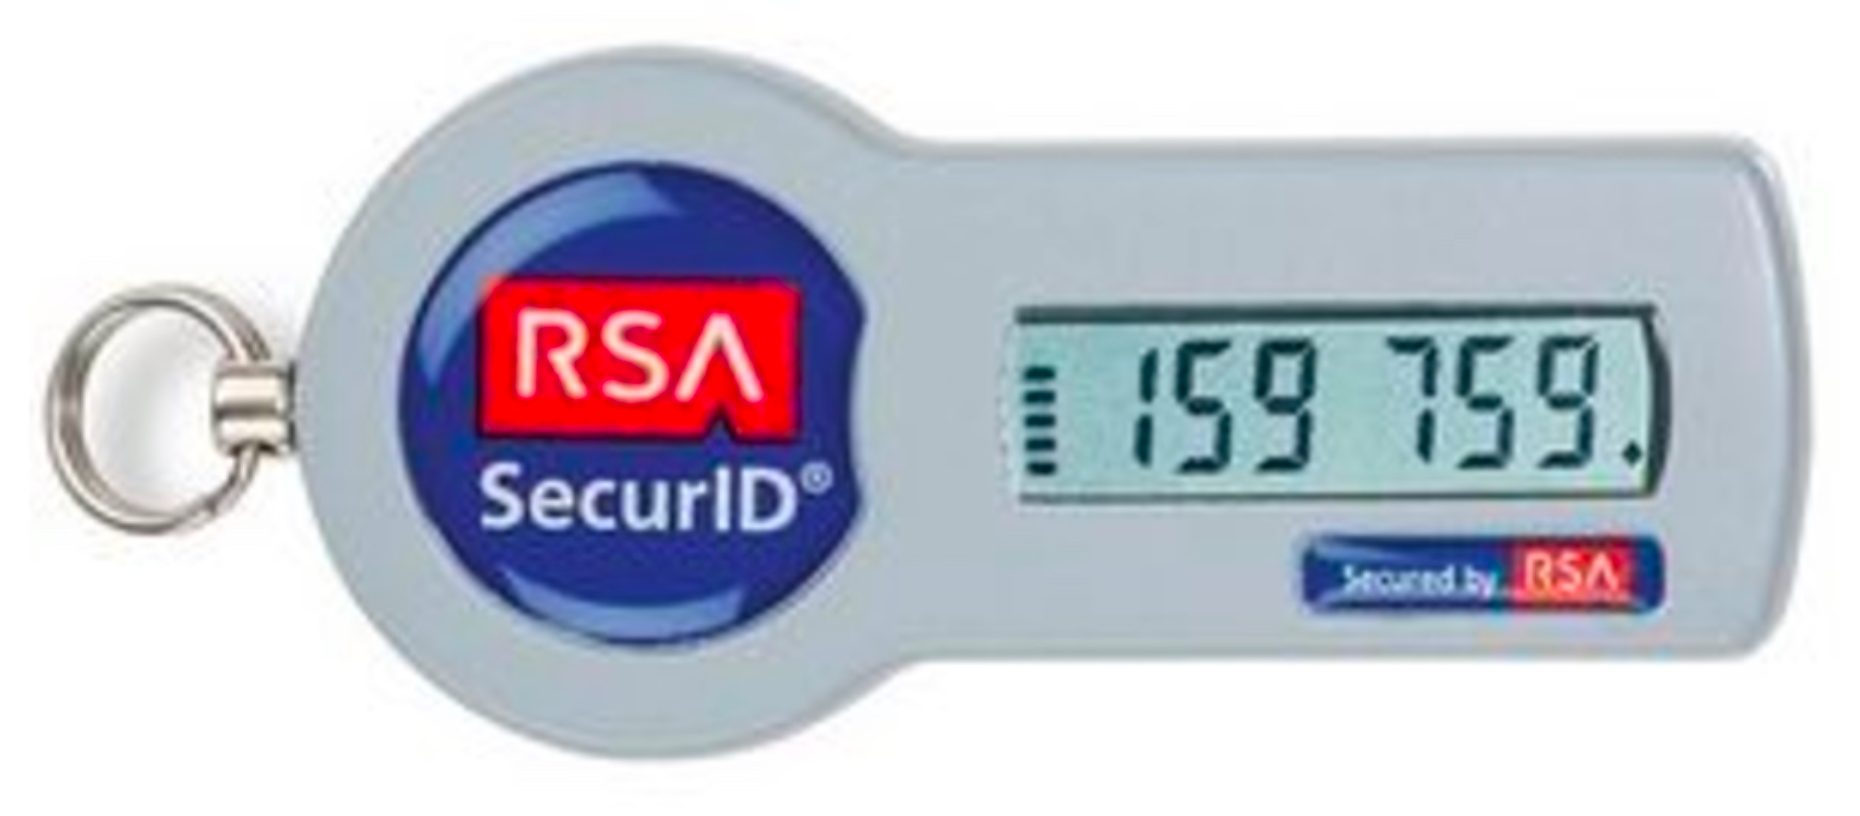
\includegraphics[width=0.3\linewidth]{figures/chapter18/fig8-a.png}
  	  \label{fig:18-8-a}
  }
  \qquad\qquad\qquad\qquad
  \subfigure[Google 认证器]{
      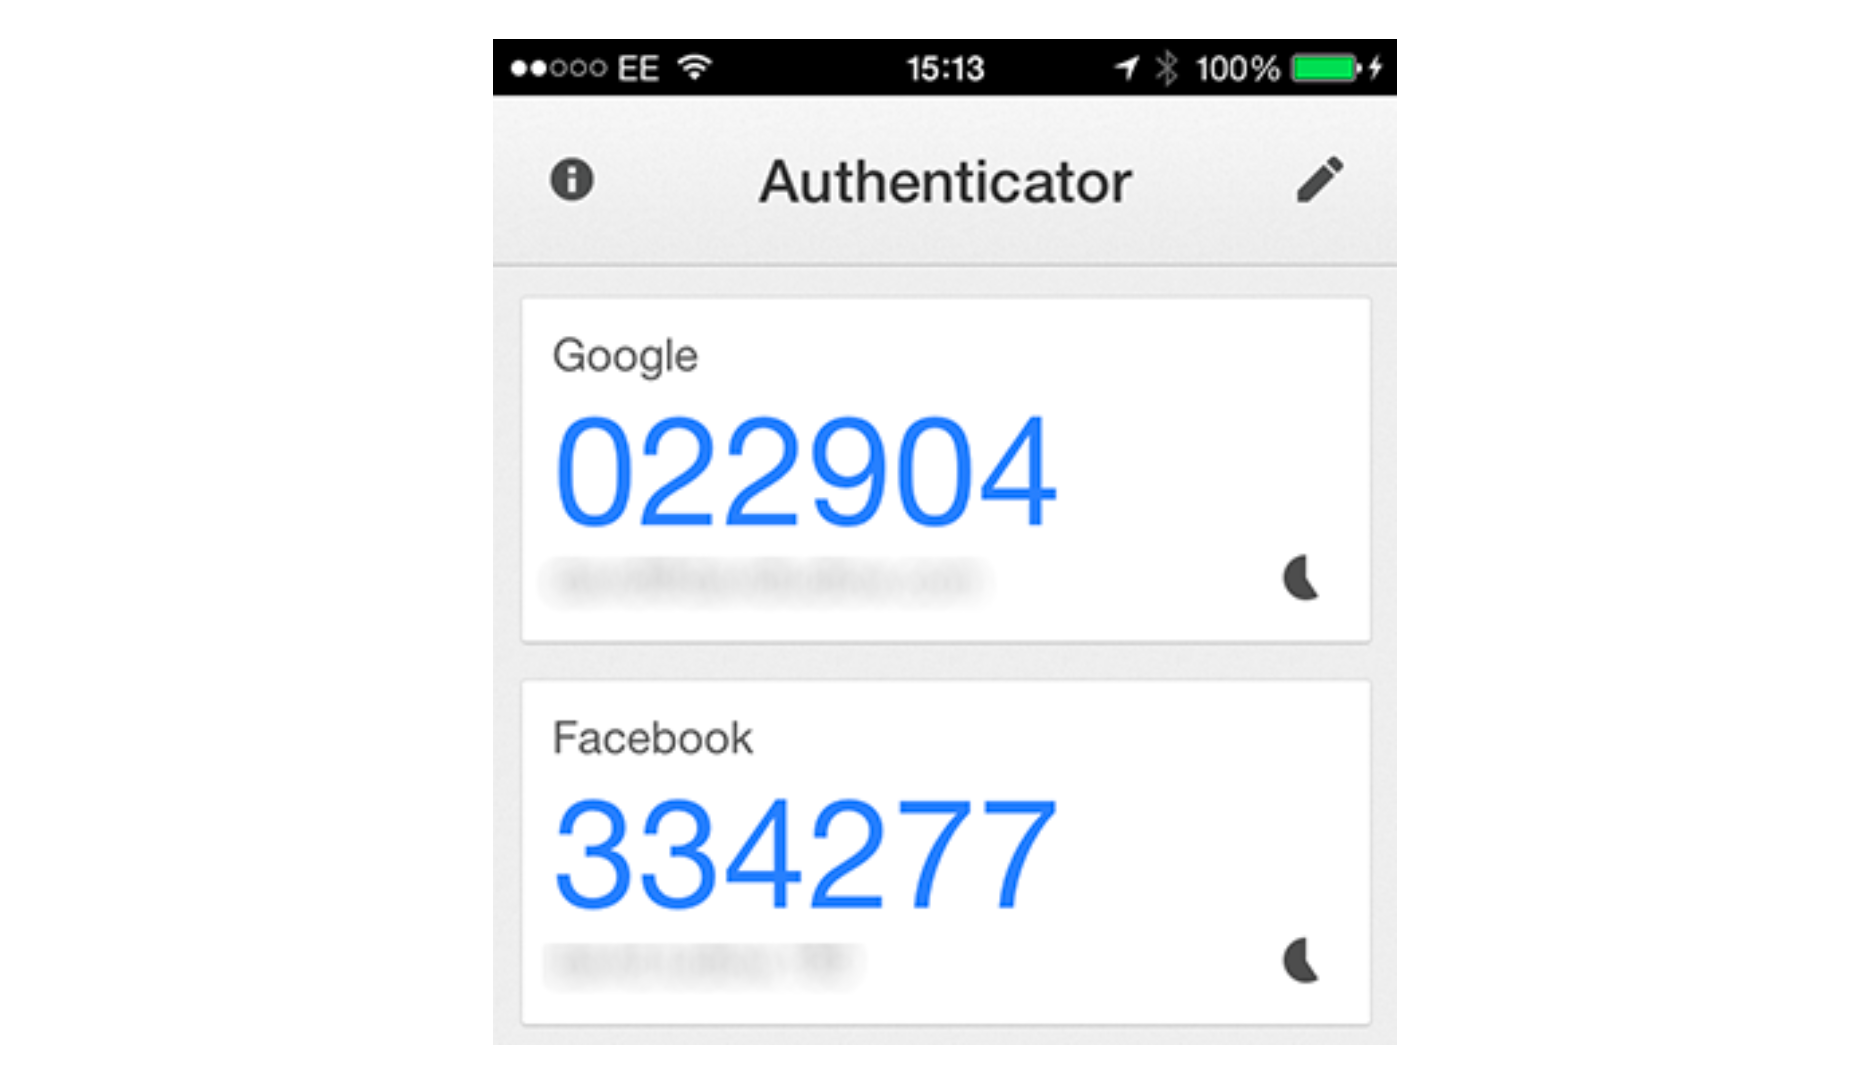
\includegraphics[width=0.3\linewidth]{figures/chapter18/fig8-b.png}
      \label{fig:18-8-b}
  }
  \caption{TOTP实现}
  \label{fig:18-8}
\end{figure}

\begin{theorem}\label{theo:18-4}
令 $F$ 是一个定义在 $(\mathcal{K},\mathbb{Z}_N,\mathcal{Y})$ 上的安全的 PNF,其中 $N$ 和 $|\mathcal{Y}|$ 都是超多项式的。那么,ID 协议 \texttt{HOTP} 对窃听是弱安全的。
\end{theorem}

\begin{proof}[证明简述]
由于 $F$ 是一个安全的 PRF,那么在攻击游戏 \ref{game:18-2} 中,对手无法区分使用 PRF 的挑战者和使用随机函数 $f:\mathbb{Z}_N\to\mathcal{Y}$ 的挑战者。此外,当挑战者使用随机函数 $f$ 时,冒充尝试的成功概率最大是 ${1}/{|\mathcal{Y}|}$。而由于 $|\mathcal{Y}|$ 是超多项式的,所以该值可忽略不计。此外,由于 $N$ 很大,在任何可行的攻击中,计数器的值都不会``环绕一圈"。
\end{proof}

HOTP 可以被用在汽车钥匙扣系统中,用于以无线方式解锁汽车,就像本章导言部分讨论的那样。秘密的 PRF 密钥 $k$ 会被存储在钥匙扣和汽车上。每当用户按下钥匙扣上的一个按钮时,钥匙扣就将内部计数器 $i$ 的值递增 $1$,并将得到的一次性口令连同计数器 $i$ 一起发送给汽车。需要注意的是,汽车必须确保收到的计数器值大于汽车当前的计数器值。

HOTP 也可以被远程网络服务器用于验证人类用户的身份。用户会得到一个安全令牌,它看起来就像图 \ref{fig:18-8-a} 中所展示的那样,显示一个 $6$ 位数的一次性口令。用户需要在她的网络浏览器中输入这个口令,以此向远程服务器证明身份。然后,这个一次性口令就会被发送到远程服务器上进行验证。下一次,当用户想再次向服务器提交验证时,她首先按下令牌上的一个按钮,使计数器 $i$ 增加 $1$。这就把令牌推进到下一个一次性口令,并更新屏幕上显示的 $6$ 位数的数值。

由于若干原因,HOTP 系统会带来很多问题。首先,在远程网络服务器的场景中,我们希望尽可能的减少用户需要输入的字符数。特别是,我们不希望要求用户在输入 $6$ 位口令的同时还要输入当前的计数器值。然而,在令牌和远程服务器不同步的情况下,计数器的值是必然需要同步的。如果我们能使用一个双方都知道的隐式计数器,情况将会变得更加友好。如下文所述,当前时间恰好就可以作为一个隐式的计数器。

其次,HOTP 还有一个安全性问题。在 HOTP 中,一次性口令只有在用户启动协议时才会被更新。如果用户不经常认证,比如一个月才使用一次,那么每个一次性口令都会在整个月内有效。攻击者如果以某种方式获得了用户当前的一次性口令,就可以把它卖给任何想冒充用户的人。那么,只要用户还没有对服务器发出新的认证请求,买家就可以在任何时候使用购买的口令,因为它一直是有效的。

\subsubsection{基于时间的一次性口令}\label{subsubsec:18-5-1-1}

一个更好的一次性口令方案被称为\textbf{基于时间的一次性口令 (time-based one-time password, TOTP)}。在 TOTP 中,无论用户是否认证,计数器 $i$ 都会每 $30$ 秒自增一次。这意味着,每个一次性口令都只在短时间内有效。当使用图 \ref{fig:18-8-b} 这样的硬件令牌时,显示屏每 $30$ 秒就会改变一次,并向用户展示最新的一次性口令。因此现在,令牌上并没有按钮。

每当用户向远程服务器发起认证请求时,服务器就会用当前时间来确定计数器 $i$ 的值,然后验证用户提供的 $r:=F(k,i)$ 是否正确。考虑到服务器和令牌之间的可能存在时钟偏移,服务器会接受 $\{F(k,(i-c)),\dots,F(k,(i+c))\}$ 中的任何一个口令作为有效的口令,其中 $c$ 是某个小的正整数,比如 $c=5$。在 $2c+1$ 的时钟偏移窗口内,服务器会拒绝以前使用过的口令,以此来防止重放攻击。

图 \ref{fig:18-8-a} 是 TOTP 的一个硬件令牌实现。在令牌设置时,一个秘密 PRF 密钥会被加载到令牌中,用于生成一个 $6$ 位数的一次性口令。服务器也持有相同的 PRF 密钥。硬件令牌内部有一个电池,可以为设备提供长达数年的供电。当电池耗尽时,令牌就会失效。

图 \ref{fig:18-8-b} 是一个智能手机上的 TOTP 应用程序。用户通过输入或扫描二维码将秘密 PRF 密钥加载到应用程序中。该应用可以管理用户在多个系统中的一次性口令,如图所示,该应用正在管理 Google 和 Facebook 的一次性口令。

\subsection{S/key 系统}\label{subsec:18-5-2}

TOTP 要求服务器始终保持其存储的验证密钥 $vk$ 的机密性。如果对手窃取了 $vk$ 而没有被发现,所有的安全性都会丧失。这实际上已经发生在了一些广为人知的案例中。

一个被称为 S/key 的系统取消了这种限制。然而,在 S/key 系统中,每对 $(vk,sk)$ 都只能被使用有限次,然后就必须重新生成一对新的。令 $n$ 是一个预设的多项式边界整数,比如 $n=10^6$,它表示一个数对 $(vk,sk)$ 能被使用的最大次数。

在 \ref{sec:14-3} 节中,我们曾经介绍过哈希链的概念,我们这里就要使用它。回顾一下,令 $H:\mathcal{X}\to\mathcal{X}$ 是一个函数。对于 $j\in\mathbb{Z}_{>0}$,我们用 $H^{(j)}(x)$ 表示 \textbf{$H$ 的第 $j$ 次迭代($j$-th iterate of $H$)},即 $H^{(j)}(x):=H(H(H(\cdots(x)\cdots)))$,其中 $H$ 被重复计算了 $j$ 次。我们令 $H^{(0)}(x):=x$。

\begin{snote}[S/key 协议。]
可被调用 $n$ 次的协议 $\mathtt{Skey}_n=(G,P,V)$ 运行如下:
\begin{itemize}
	\item $G$:随机选取一个 $k\overset{\rm R}\leftarrow\mathcal{X}$,输出 $sk:=(k,n)$,$vk:=H^{(n+1)}(k)$,
	\item 算法 $P$ 被赋予 $sk$,算法 $V$ 被赋予 $vk$,并按如下方式交互:
	\begin{enumerate}
		\item $P\big(sk=(k,i)\big)$:将 $t:=H^{(i)}(k)$ 发送给 $V$,并且设置 $sk\leftarrow(k,i-1)$,
		\item $V(vk)$:如果来自 $P$ 的 $t$ 满足 $vk=H(t)$,则输出 $\mathsf{accept}$,并设置 $vk\leftarrow t$。否则输出 $\mathsf{reject}$。
	\end{enumerate}
\end{itemize}
该协议如图 \ref{fig:18-9} 所示。在第一次调用时,证明者者向验证者发送口令 $H^{(n)}(k)$。在第二次调用中,证明者会发送 $H^{(n-1)}(k)$,以此类推。每个口令都只能使用一次。显然,经过 $n$ 次调用后,证明者的一次性口令就用完了,这时,证明者就不能再向验证者认证了,必须生成一个新的 $(vk,sk)$ 对。
\end{snote}

\begin{figure}
  \centering
  \input{figures/chapter18/fig9.tex}
  \caption{S/key 协议}
  \label{fig:18-9}
\end{figure}

\begin{snote}[S/key 的安全性。]
我们声称,即使 $vk$ 被公开了,S/key 仍然是安全的。因此,S/key 对窃听是完全安全的,相比之下,\texttt{HOTP} 只是弱安全的。

对 S/key 的分析要求 $H:\mathcal{X}\to\mathcal{X}$ 在 $n$ 次迭代中都是 \ref{def:14-5} 意义上的单向函数。回顾一下,这意味着,对于所有的 $j=1,\dots,n$,给定 $y\leftarrow H^{(j)}(k)$ 作为输入,其中 $k\overset{\rm R}\leftarrow\mathcal{X}$,都很难找到一个 $H^{-1}(y)$ 中的元素。回顾一下,我们在练习 \ref{exer:14-15} 中表明,一个单向函数 $H$ 在 $n$ 次迭代中不一定是单向的,就算 $n=2$ 也是如此。然而,标准的密码学哈希函数,如 SHA256,在合理的 $n$ 值上确实是单向的,比如 $n\leq 10^{6}$ 时。
\end{snote}

\begin{theorem}\label{theo:18-5}
令 $H:\mathcal{X}\to\mathcal{X}$ 是一个 $n$ 次迭代上的单向函数。则身份识别协议 $\mathtt{Skey}_n$ 对窃听是安全的。
\end{theorem}

\begin{proof}[证明简述]
既然 $vk$ 是公开的,我们就可以假设对手窃听了多次(比如说 $Q$ 次)对话,然后进行了一次冒充尝试。我们事先不知道 $Q$ 是多少,但我们可以猜测它的值。我们从迭代的单向挑战者那里请求 $y\leftarrow H^{(n-Q+1)}(k)$,并使用 $y$ 来生成与初始验证密钥 $vk=H^{(n+1)}(k)$ 有关的 $Q$ 个有效对话。如果我们对 $Q$ 的猜测是正确的,并且对手成功地进行了冒充尝试,对手将为我们找到 $y$ 的原像。因此,如果对手能以概率 $\epsilon$ 成功冒充,我们就能以 $\epsilon/n$ 的概率赢得攻击游戏 \ref{game:14-1}。
\end{proof}

\begin{remark}\label{remark:18-1}
为了防御如 \ref{sec:18-7} 节所讨论的那类针对 $H$ 的预处理攻击,算法 $G$ 可以在设置时选择一个公共盐,并在每次评估 $H$ 时都将这个盐作为前缀添加到输入中。此外,为了避免 \ref{exer:14-17} 中所示的攻击,我们建议在哈希链的每一步中都使用不同的哈希函数。\cite{kogan2017t} 分析了这种防御。
\end{remark}

\begin{snote}[S/key 的麻烦。]
在每次认证尝试中,验证者 $P$ 都必须向 $V$ 发送一个元素 $t\in\mathcal{X}$。为了使 $H$ 是单向的,集合 $\mathcal{X}$ 必须很大,因此 $t$ 不能像 TOTP 系统中那样是一个 $6$ 位数。在实践中,$t$ 至少需要有 $128$ 位,以确保 $H$ 是单向的。这使得,当使用 S/key 作为一次性口令方案时,用户需要手动输入口令,这是很不方便的。将一个 $128$ 位的 $t$ 编码为可打印的字符,至少需要 $22$ 个字符。
\end{snote}
\section{挑战-应答:针对主动攻击的安全性}\label{sec:18-6}


现在,我们来考虑一种更强大的攻击,在这种攻击中,对手会主动地冒充合法的验证者。比如说,对手可以克隆一个银行网站,等待用户(即证明者)访问该网站,并与对手一起运行 ID 协议。这样一来,对手就可以反复与用户交互,并向用户发送其选择的任意消息。对手的目标是获得关于验证者密钥 $sk$ 的信息。经过几次这样的交互,对手就转过身来,试图以证明者的身份向合法的验证者发起认证请求。如果对手仍然无法欺骗验证者,我们就称 ID 协议对主动攻击是安全的。

\ref{sec:18-5} 节中介绍的一次性口令协议 \texttt{HOTP} 和 \texttt{Skey} 对主动攻击显然是不安全的。通过冒充验证者,对手能从证明者那里学到新的一次性口令,对手可以用这个口令来向验证者发起认证请求。事实上,只要简单思考,我们就可以发现,没有任何一个单向流协议足以抵御主动攻击。

下面,我们首先给出主动攻击的严格定义,然后构建一个简单的双向流协议,它对主动攻击是安全的。简单起见,在本节中,我们只考虑证明者和验证者都是无状态的协议。

\begin{game}[安全的身份识别:主动攻击]\label{game:18-3}
对于一个给定的身份识别协议 $\mathcal{I}=(G,P,V)$ 和一个给定的对手 $\mathcal{A}$,攻击游戏如图 \ref{fig:18-10} 所示,运行如下:
\begin{itemize}
	\item \emph{密钥生成阶段。}挑战者运行 $(vk,sk)\overset{\rm R}\leftarrow G()$,然后将 $vk$ 发送给对手 $\mathcal{A}$。
	\item \emph{主动探测阶段。}对手请求与证明者进行交互。挑战者与对手在 ID 协议中交互,它扮演证明者的角色,运行算法 $P$,该算法以 $sk$ 初始化。对手扮演验证者的角色,但它不一定遵循验证者的算法 $V$。对手可以与证明者的许多实例并行交互,这些交互可以任意地相互交错进行。
	\item \emph{冒充尝试。}如攻击游戏 \ref{game:18-1} 中一样,挑战者与 $\mathcal{A}$ 交互。挑战者遵循验证者的算法 $V$(以 $vk$ 为输入),而对手 $\mathcal{A}$ 会扮演证明者的角色,但不一定会遵循证明者的算法 $P$。
\end{itemize}
如果验证协议 $V$ 在交互结束时输出 $\mathsf{accept}$,我们就称对手 $\mathcal{A}$ 赢得了游戏。我们将 $\mathcal{A}$ 就 $\mathcal{I}$ 的优势定义为 $\mathrm{ID3}\mathsf{adv}[\mathcal{A}, \mathcal{I}]$,即 $\mathcal{A}$ 赢得游戏的概率。
\end{game}

\begin{figure}
  \centering
  \input{figures/chapter18/fig10.tex}
  \caption{攻击游戏 \ref{game:18-3} 中主动攻击的例子}
  \label{fig:18-10}
\end{figure}

\begin{definition}\label{def:18-8}
如果对于所有的有效对手 $\mathcal{A}$,$\mathrm{ID3}\mathsf{adv}[\mathcal{A}, \mathcal{I}]$ 的值都可忽略不计,我们就称身份识别协议 $\mathcal{I}$ \textbf{对主动攻击是安全的(secure against active attacks)}。
\end{definition}

\begin{snote}[并行攻击 vs. 串行攻击。]
请注意,在攻击游戏的主动探测阶段,我们允许对手同时与证明者的多个实例交互。我们可以考虑一个较弱的攻击模型,在该模型中,这些交互必须按顺序运行,如图 \ref{fig:18-10} 所示。然而,我们考察的所有协议都能在这种更强的、并行的攻击模型中保持安全性。
\end{snote}

\begin{snote}[保持 $vk$ 的机密性。]
一些满足定义 \ref{def:18-8} 的协议并不要求验证者保有任何秘密。然而,我们将要在本节介绍的一个协议确实要求 $vk$ 是秘密的。这就促成了攻击游戏 \ref{game:18-3} 的一个弱化版本,即挑战者不向对手发送 $vk$。正如 \ref{sec:18-5} 节所述,如果 $vk$ 是保密的,我们就必须允许对手与验证者交互,因为这种交互有可能泄露 $vk$ 的信息。因此,在主动探测阶段,我们允许对手同时与证明者和验证者的多个实例交互。当与一个验证者实例交互时,对手会了解验证者输出的是 $\mathsf{accept}$ 还是 $\mathsf{reject}$。此外,在冒充尝试期间,我们让对手同时与多个验证者交互,如果这些验证者中至少有一个接受,对手就赢得了游戏。

我们令 $\mathrm{wID3}\mathsf{adv}[\mathcal{A},\mathcal{I}]$ 为对手赢得这个较弱版本的攻击游戏 \ref{game:18-3} 的优势。在这种设置下安全的身份识别协议被称为是\textbf{弱安全的(weakly secure)}。
\end{snote}

\begin{definition}\label{def:18-9}
如果对于所有的有效对手 $\mathcal{A}$,$\mathrm{wID3}\mathsf{adv}[\mathcal{A},\mathcal{I}]$ 的值都可忽略不计,我们就称 ID 协议 $\mathcal{I}$ \textbf{对主动攻击是弱安全的(weakly secure against active attacks)}。
\end{definition}

\subsection{挑战-应答协议}\label{subsec:18-6-1}

我们介绍两种(无状态)ID 协议,称为\textbf{挑战-应答(challenge-response)},对主动攻击都是安全的。第一种协议是弱安全的,即验证者必须保密 $vk$。对于第二种协议,即使 $vk$ 被公开,它也是安全的。

令 $\mathcal{I}=(S_\mathrm{mac},V_\mathrm{mac})$ 是一个定义在 $(\mathcal{K},\mathcal{M},\mathcal{T})$ 上的 MAC。挑战-应答协议 $\mathtt{ChalResp}_\mathrm{mac} = (G,P,V)$ 如图 \ref{fig:18-11} 所示,运行如下:
\begin{itemize}
	\item $G$:随机选取一个 $k\overset{\rm R}\leftarrow\mathcal{K}$ 并输出 $sk:=k$ 和 $vk:=k$。
	\item 算法 $P$ 被赋予 $sk$,算法 $V$ 被赋予 $vk$,并按如下方式交互:
	\begin{enumerate}
		\item $V$ 随机选取一个 $c\overset{\rm R}\leftarrow\mathcal{M}$,并将 $c$ 发送给 $P$;
		\item $P$ 计算 $t\overset{\rm R}\leftarrow S_\mathrm{mac}(k,c)$,并将 $t$ 发送给 $V$;
		\item $V$ 输出 $V_\mathrm{mac}(k,c,t)$。
	\end{enumerate}
\end{itemize}
随机数 $c$ 被称为\textbf{挑战 (challenge)},$t$ 被称为\textbf{应答 (response)}。显然,为了保证协议的安全性,$vk$ 必须保密。

\begin{figure}
  \centering
  \input{figures/chapter18/fig11.tex}
  \caption{基于 MAC 的挑战-应答身份识别}
  \label{fig:18-11}
\end{figure}

\begin{theorem}\label{theo:18-6}
假设 $\mathcal{I}$ 是一个安全的 MAC 系统,并且消息空间的大小 $|\mathcal{M}|$ 是超多项式的。那么 ID 协议 $\mathtt{ChalResp}_\mathrm{mac}$ 对主动攻击是弱安全的。
\end{theorem}

\begin{proof}[证明简述]
如果 $|\mathcal{M}|$ 是超多项式的,就意味着,在每次冒充尝试中,对手收到它之前(在与证明者的交互中)见过的挑战消息的概率可忽略不计。因此,要么这种小概率事件发生,要么对手(在攻击游戏 \ref{game:6-2} 的意义上)攻破了 MAC 系统。
\end{proof}

\begin{figure}
  \centering
  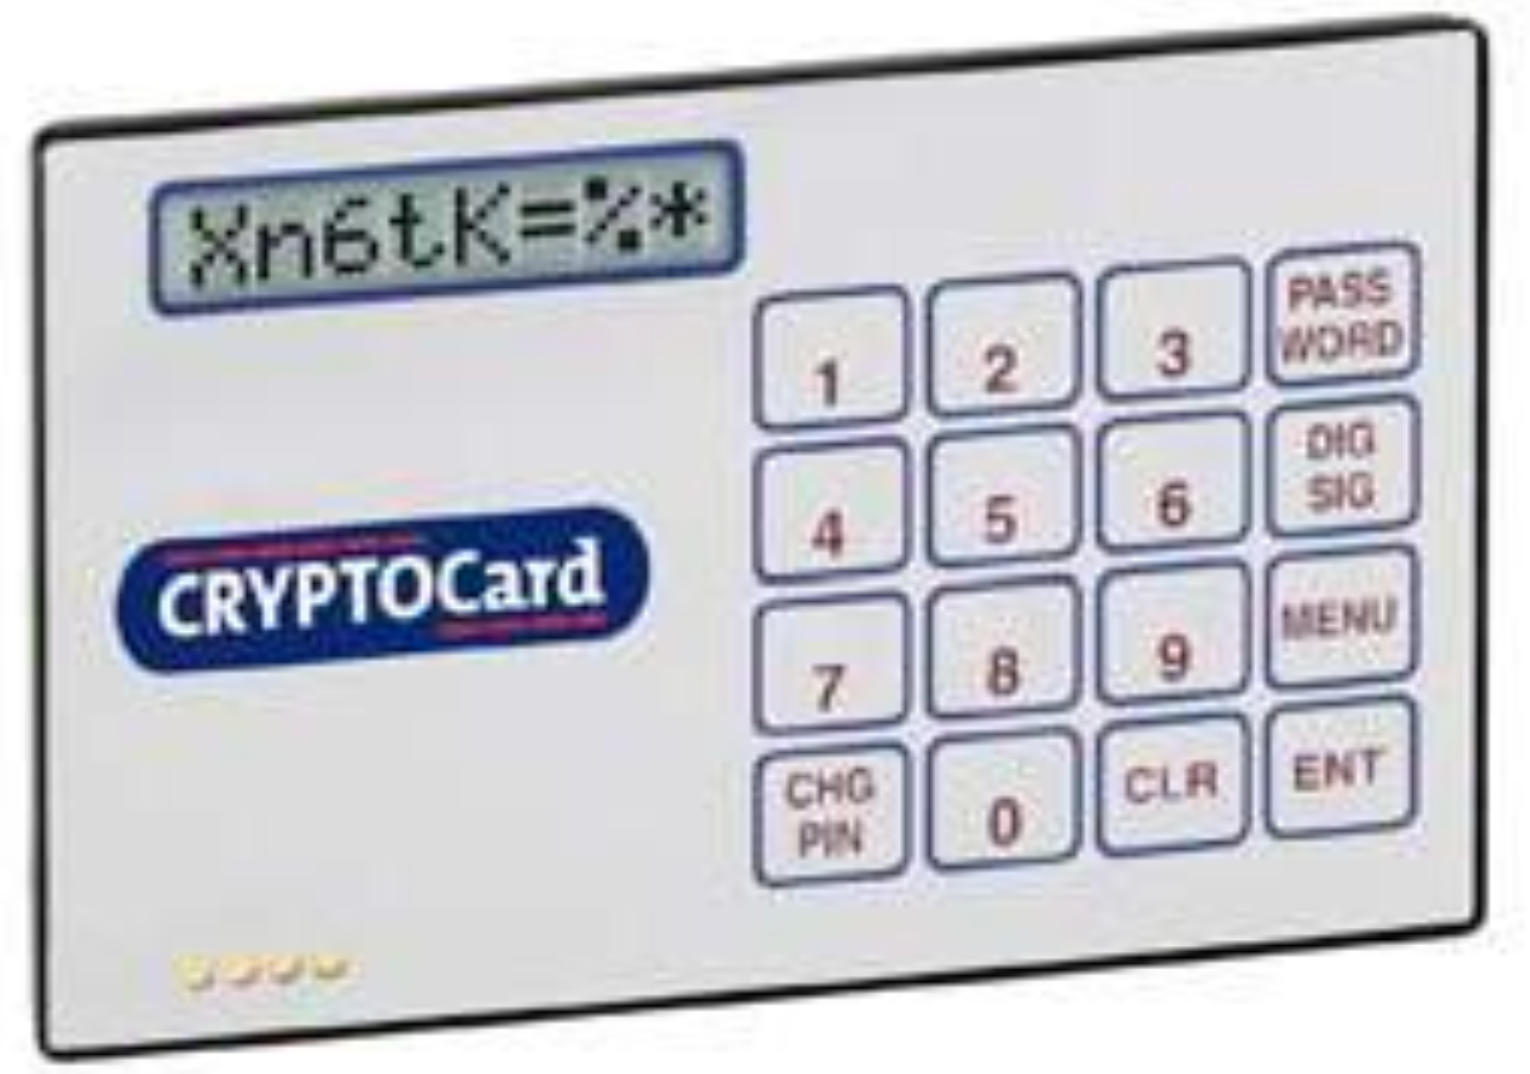
\includegraphics[width=0.25\linewidth]{figures/chapter18/fig12.png}
  \caption{CRYPTOCard RB-1 令牌}
  \label{fig:18-12}
\end{figure}

\begin{snote}[案例研究:CRYPTOCard。]
图 \ref{fig:18-12} 给出了一个挑战-应答令牌的例子。当用户使用他的计算机终端登录到服务器时,服务器会向用户发送一个 $8$ 字符的挑战,该挑战会出现在他的计算机终端屏幕上。用户使用令牌上的小键盘将这个挑战输入令牌。令牌计算出响应,并显示在其屏幕上。然后,用户在他的计算机终端上输入这个响应,并将其发送到服务器,以完成协议。MAC 由一个派生自 3DES 或 AES 的 PRF 实现。
\end{snote}

\begin{snote}[使用口令的挑战-应答。]
在描述协议 $\mathtt{ChalResp}_\mathrm{mac}$ 时,密钥 $k$ 是从底层 MAC 系统的密钥空间 $\mathcal{K}$ 中随机选出的。在某些情况下,部署下面这样的协议是很方便的,它的密钥 $k$ 是由用户生成的口令 $pw$ 推导出来的,比如 $k\leftarrow H(pw)$,其中的 $H$ 是一个 \ref{sec:8-10} 节中介绍的密钥派生函数。

但这可能是相当危险的。如果 $pw$ 是一个弱口令,并且被包含在了某个相对较小的常用密码字典 $\mathcal{D}$ 中,这个协议就很容易受到简单的离线字典攻击。在窃听了证明者和验证者之间单独的某一次对话 $(c,t)$ 后,对手可以进行如下操作:

\vspace*{10pt}

\hspace*{5pt} 对于每个 $w\in\mathcal{D}$:\\
\hspace*{50pt} 如果 $V_\mathrm{mac}\big(H(w),c,t\big)= \mathsf{accept}$:\\
\hspace*{75pt} 输出 $w$ 并停机

\vspace*{10pt}

\noindent
这样,输出的极有可能就是口令 $pw$。
\end{snote}

\subsubsection{使用公开 $vk$ 的挑战应答}\label{subsubsec:18-6-1-1}

图 \ref{fig:18-11} 中的协议很容易转化为 $vk$ 可公开的协议。我们只需用一个定义在 $(\mathcal{M},\mathcal{T})$ 上的签名方案 $(G,S_\mathrm{sig},V_\mathrm{sig})$ 替换 MAC。对 \ref{fig:18-11} 的主要变化是,证明者现在使用算法 $S_\mathrm{sig}$ 和签名私钥来应答挑战。验证者使用算法 $V_\mathrm{sig}$ 和验证公钥来验证应答。我们将所产生协议称为 $\mathtt{ChalResp}_\mathrm{sig}$。

\begin{theorem}\label{theo:18-7}
假设 $\mathcal{S}$ 是一个安全的签名方案,并且消息空间的大小 $|\mathcal{M}|$ 是超多项式的。那么 $\mathtt{ChalResp}_\mathrm{sig}$ 对主动攻击是安全的。
\end{theorem}

\begin{proof}[证明简述]
证明思路与定理 \ref{theo:18-6} 基本相同,只是现在,对手需要伪造的是一个签名,而不是 MAC。
\end{proof}

基于签名的挑战-应答协议拥有明显优于基于 MAC 的挑战-应答协议的安全优势,因为 $vk$ 不需要保密。然而,基于 MAC 的协议的优点在于,它的应答消息可以很短,这对于类似 CRYPTOCard 的应用来说是至关重要的,因为在这种应用中,用户必须在键盘上输入挑战和应答。回顾一下,在 CRYPTOCard 中,应答消息只有 $48$ 比特长。而一个数字签名方案不可能即是安全的,又是短签名的。练习 \ref{exer:18-13} 探讨了另一种挑战-应答协议,在这种协议中,应答消息可以是很短的。
\section{一个有趣的应用:彩虹表}\label{sec:18-7}

令 $h:\mathcal{P}\to\mathcal{Y}$ 是一个随机函数,并设置 $N:=|\mathcal{P}|$。我们来看看计算 $h$ 的逆这个一般的问题。我们假设 $|\mathcal{Y}|\geq N$,因为这是实践中的典型情况。比如说,$\mathcal{P}$ 可能是所有 $8$ 字符口令的集合,而 $\mathcal{Y}=\{0,1\}^{256}$。

令 $pw\overset{\rm R}\leftarrow\mathcal{P}$,并令 $y\leftarrow h(pw)$。显然,对 $\mathcal{P}$ 的所有可能性进行穷举搜索,只要对 $h$ 进行最多 $N$ 次查询,就可以确保找到 $y$ 的原像。在本节中,我们将开发一种更快的算法,它使用一种称作\textbf{彩虹表(rainbow table)}的方法来求取 $h$ 的逆。求逆算法 $\mathcal{A}=(\mathcal{A}_0,\mathcal{A}_1)$ 分两个阶段进行:
\begin{itemize}
	\item 预处理阶段:算法 $\mathcal{A}_0$ 查询 $h$,并输出一张包含 $\ell$ 个 $\mathcal{P}^2$ 中的数对的表 $L$,其中 $\ell$ 是某个正整数。该预处理阶段耗时为 $O(N)$,但它在获知挑战 $y$ 之前已被离线完成。产生的表 $L$ 被称为彩虹表,它必须被妥善储存,以便在第二阶段使用。
	\item 攻击阶段:一旦被赋予一个挑战 $y\in\mathcal{Y}$,$\mathcal{A}_1$ 算法就会以 $\mathcal{A}_1(L,y)$ 的方式被调用,使用 $L$ 快速地找到 $y$ 的逆元。它能以接近 $1$ 的概率输出一个 $h^{-1}(y)$ 中的原像 $pw'$。
\end{itemize}
令 $t$ 为 $\mathcal{A}_1$ 在攻击阶段中的运行时间。下面,我们展示如何在时间 $t$ 内计算 $h$ 的逆,其中:
\begin{equation}\label{eq:18-9}
t\times\ell^2\approx N^2
\end{equation}
举例来说,如果我们可以存储一个大小为 $\ell=N^{2/3}$ 的表 $L$,我们就可以在 $t\approx N^{2/3}$ 的时间内以接近 $1$ 的概率计算 $h$ 的逆,这比在 $\mathcal{P}$ 上进行穷举搜索要快得多。

式 \ref{eq:18-9} 被称作\textbf{时空权衡(time-space tradeoff)}。我们留给表 $L$ 的空间越大,求取 $h$ 的逆的速度就越快。当然,一旦我们有了表 $L$,我们就可以用它来快速地找到许多 $\mathcal{Y}$ 中元素的逆。

正如 \ref{subsubsec:18-3-1-3} 小节所述,彩虹表通常被用于破解未加盐的口令。它们也可以用于从已知的明文-密文对 $\big(m,\,c=E(k,m)\big)$ 中恢复分组密码 $(E,D)$ 的秘钥 $k$。这是因为密钥 $k$ 就是函数 $h(k):=E(k,m)$ 在 $c$ 点处的逆元。如果 $m$ 足够长,或者提供足够多的明文-密文对,那么这个逆元 $k$ 就是唯一的。将此结论应用于 AES-128,我们就可以得到一个大小为 $128\times(2^{128})^{(2/3)}\approx 128\times 2^{85}$ 比特的表 $L$(约 $10$ 亿艾字节),它可以被用来在 $2^{85}$ 的时间内破解 AES。它的耗时在今天来看可能太长,但在几十年后可能会变得可以接受。我们曾在第 \ref{subsubsec:4-2-2-1} 小节中讨论过这种威胁。这种威胁也是迫使人们转向 AES-256 的一个很重要的原因。但是请注意,建立表 $L$ 需要大量(一次性的)工作,即大约 $2^{128}$ 次对 AES-128 的评估。

细心的读者会注意到,式 \ref{eq:18-9} 中的边界在 $\ell=1$ 时相当差,此时,我们有 $t\approx N^2$。这比耗时为 $N$ 的简单穷举搜索还要差得多。这说明,彩虹表算法对于某些 $\ell$ 值来说并不严格。改进时空权衡 \ref{eq:18-9} 是一个长期存在的开放性问题(见练习 \ref{exer:18-7})。

\begin{snote}[Hellman 的基本时空权衡。]
第一个用于求取随机函数的逆的时空权衡是由 Hellman 发明的,它是对 DES 的短密钥设计($56$ 比特)的一个有力批评。Hellman 的方法使用了一个可有效计算的辅助函数 $g:\mathcal{Y}\to\mathcal{P}$,被称为\textbf{还原函数(reduction function)}。它能将 $h$ 的一个 $\mathcal{Y}$ 上的输出``还原"为一个 $\mathcal{P}$ 上的元素。简单起见,我们假设 $g$ 也是一个随机函数。那么,函数 $f(pw):=g(h(pw))$ 就会将 $\mathcal{P}$ 映射到它自身。

预处理算法 $\mathcal{A}_0$ 使用函数 $f:\mathcal{P}\to\mathcal{P}$,它以两个正常数 $\tau$ 和 $\ell$ 为参数。回顾一下,对于 $\tau>0$,函数 $f^{(\tau)}$ 就是定义在 \ref{eq:18-5} 中的 $f$ 的 $\tau$ 次迭代。图 \ref{fig:18-13-a} 直观地展示了算法 $\mathcal{A}_0$ 的工作原理,它运行如下:

\vspace*{10pt}

\hspace*{5pt} 算法 $\mathcal{A}_0$:(预处理 $h$)\\
\hspace*{50pt} 对于 $i=1,\dots,\ell$:\\
\hspace*{75pt} 随机选取 $pw_i\overset{\rm R}\leftarrow\mathcal{P}$\\
\hspace*{75pt} 令 $z_i\leftarrow f^{(\tau)}(pw_i)\in\mathcal{P}$
\hspace*{100pt} // \emph{对 $f$ 进行 $\tau$ 次评估}

\vspace*{5pt}

\hspace*{28.5pt} 输出 $L:=\big\{(pw_1,z_1),\dots,(pw_\ell,z_\ell)\big\}\subseteq\mathcal{P}^2$
\hspace*{37pt} // \emph{输出 $\ell$ 个 $\mathcal{P}^2$ 中的数对}

\vspace*{10pt}

\begin{figure}
  \centering
  \subfigure[Hellman 的基本时空权衡]{
  	  \input{figures/chapter18/fig13-a.tex}
  	  \label{fig:18-13-a}
  }
  \subfigure[彩虹表]{
      \input{figures/chapter18/fig13-b.tex}
  	  \label{fig:18-13-b}
  }
  \caption{时空权衡表,方框内的表项组成了表 $L$。}
  \label{fig:18-13}
\end{figure}

算法 $\mathcal{A}_0$ 建立了 $\ell$ 条水平方向的链,如图 \ref{fig:18-13-a} 所示。对于每条链,表 $L$ 都会记录其起点和终点,其运行时间与 $\tau\times\ell$ 成正比。

接下来,为了使用 $L$ 计算元素 $y\in\mathcal{Y}$ 的逆,我们重复地将 $f$ 作用于 $g(y)$,直到抵达图 \ref{fig:18-13-a} 的最右侧。然后,我们使用 $L$ 跳跃到相关链的起点,并遍历它,直到我们找到 $y$ 的原像。更确切地说,为了计算 $y$ 的逆,我们进行以下操作:

\vspace*{10pt}

\hspace*{5pt} 算法 $\mathcal{A}_1(L,y)$:\\
\hspace*{26pt} 1. \quad 令 $z\leftarrow g(y)\in\mathcal{P}$\\
\hspace*{26pt} 2. \quad 对于 $i=1,\dots,\tau$:\\
\hspace*{26pt} 3. \quad\qquad 如果存在某个 $\widetilde{pw}$ 使得 $(\widetilde{pw},z)\in L$:
\hspace*{20pt} // \emph{如果 $z$ 是一条链的终点} \\
\hspace*{26pt} 4. \quad\qquad\qquad 令 $pw\leftarrow f^{(\tau-i)}(\widetilde{pw})$
\hspace*{73.5pt} // \emph{从起点开始遍历链} \\
\hspace*{26pt} 5. \quad\qquad\qquad 如果 $h(pw)=y$:
\hspace*{87pt} // \emph{如果发现逆元,将其输出} \\
\hspace*{116pt} 输出 $pw$ 并终止\\
\hspace*{26pt} 6. \quad\qquad 令 $z\leftarrow f(z)\in\mathcal{P}$
\hspace*{109pt} // \emph{将链下移} \\
\hspace*{26pt} 7. \quad 输出 $\mathsf{fail}$
\hspace*{168.5pt} // \emph{$g(y)$ 不在任何一条链上}

\vspace*{10pt}

如果图片看起来像图 \ref{fig:18-13-a},那么 $g(y)$ 就会出现在其中一条链的某处,就像图中所展示的那样。一旦我们找到这条链的终点,表 $L$ 就会给出其起点 $pw$。第 $4$ 行的遍历将会给出 $y$ 的逆。求取 $y$ 的逆的总运行时间就是对 $f$ 进行 $\tau$ 次评估和对 $L$ 进行 $\tau$ 次查询的总耗时。

然而,有时情况可能会更复杂一些。图 \ref{fig:18-13-a} 忽略了链之间发生碰撞的可能性,如图 \ref{fig:18-14} 所示。在该图中,第一条链和第二条链发生了碰撞,因为 $f^{(4)}(pw_1)=f^{(6)}(pw_2)$。第二条链和第三条链也发生了碰撞,因为 $f^{(5)}(pw_2)=f^{(7)}(pw_3)$。输入的 $g(y)$ 恰好位于顶部的链上。当我们从 $g(y)$ 开始,沿着顶上这条链移动时,我们首先找到了第三条链的终点 $z_3$,然后是第二条链的终点 $z_2$,最后才是第一条链的终点 $z_1$,后者让我们可以反转 $y$。这就是为什么在第 $5$ 行,我们必须在输出之前检查我们是否已经找到了 $y$ 的逆,以避免误报导致我们遍历错误的链。在图\ref{fig:18-14} 中,$z_3$ 和 $z_2$ 都会引起误报。此外,当 $g(h(pw))=g(y)$ 但 $h(pw)\neq y$ 时,误报也有可能发生,这也是第 $5$ 行检验的另一个原因。
\end{snote}

\begin{snote}[链合并问题。]
尽管 Hellman 的基本方法相当巧妙,但它并不能如描述的那样工作,几乎所有对 $y=h(pw)$ 逆的计算都会失败。让我们来看看原因。要使 $\mathcal{A}_1$ 成功,我们需要确保几乎所有的 $pw\in\mathcal{P}$ 都在至少一条链上。$\mathcal{A}_0$ 能够处理的最大口令有 $\tau\times\ell$ 条。因此,我们至少需要 $\tau\times\ell\geq N$。为了获得最佳性能,我们应该设置 $\tau\times\ell=N$,并希望 $\mathcal{P}$ 中的大多数 $pw$ 都在某条链上。

事实证明,这并不可行。一旦两条链发生碰撞,它们就会合并并且覆盖相同的元素,如图 \ref{fig:18-14} 所示。在建立一张有大量长链的表时,链的合并是不可避免的,并且经常发生。为了说明这个问题的严重性,我们不妨取 $\tau=N^{1/3}$,$\ell=N^{2/3}$,则 $\tau\times\ell=N$。令 $A$ 是预处理过程中遭遇的所有 $\mathcal{P}$ 上元素的集合。如果我们将 $f:\mathcal{P}\to\mathcal{P}$ 建模为一个随机函数,我们就可以证明,集合 $A$ 不太可能包含超过 $o(N)$ 个 $\mathcal{P}$ 上的元素。这意味着,当 $N$ 趋近于无穷大时,$|A|/N$ 趋近于 $0$,因而算法 $\mathcal{A}_1(L,y)$ 对于几乎所有的 $y=h(pw)$ 都会失败。事实上,为了捕获 $\mathcal{P}$ 的一个恒定比例的部分,我们需要 $\ell=\Omega(N)$ 条长度为 $\tau$ 的链。这将使得表 $L$ 的大小也是 $\Omega(N)$,这又使得这种时空权衡失去意义:有一个这么大的表,我们可以在恒定时间内轻而易举地计算 $h$ 的逆。

Hellman 对这个问题的解决方案是建立许多独立的小表,每张表使用不同的还原函数 $g$。每个表包含少量长度为 $τ$ 的链,这确保在单张表内不会发生碰撞。算法 $\mathcal{A}_1$ 分别在每张表中进行搜索,因此,如果有 $m$ 张表的话,运行速度就会慢 $m$ 倍。这样做效果很好,能够达到式 \ref{eq:18-9} 中的约束。然而,另一种被称为彩虹表的解决方案更为简单高效。
\end{snote}

\begin{figure}
  \centering
  \input{figures/chapter18/fig14.tex}
  \caption{一个链碰撞实例,三条链的长度都是 $10$}
  \label{fig:18-14}
\end{figure}

\begin{snote}[彩虹表。]
链合并问题的一个优雅的解决方案是为图 \ref{fig:18-13-a} 的每一列 $i=1,\dots,\tau$ 使用不同的还原函数 $g_i:\mathcal{Y}\to\mathcal{P}$。和之前一样,令 $f_i(pw)= g_i(h(pw))$。预处理算法 $\mathcal{A}_0$ 现在执行图 \ref{fig:18-13-b} 中的流程。它输出一张与之前相同的表 $L$,该表包含每条链的起点和终点。如果把每条链染上不同的颜色,然后将它们略微向上弯曲,图片看起来就像是一道彩虹,这就是它名字的由来。

在每一列中使用不同的函数 $f_i$ 的意义在于,链的碰撞不一定会导致链的合并。只有当两条链在完全相同的索引处发生碰撞时,它们才会合并。这使得链合并的概率大大降低(见练习 \ref{exer:18-18})。此外,如果一条以 $pw$ 为起点的链恰好与一条以 $pw'$ 为起点的链合并,这两条链的终点 $z$ 和 $z'$ 也会是相等的。预处理算法 $\mathcal{A}_0$ 可以很容易地检测到这种重复的终点,并丢弃掉其中的一条链。最终的结果是,我们可以设定 $\tau=N^{1/3}$,$\ell=N^{2/3}$,并在预处理过程中捕获 $\mathcal{P}$ 的一个恒定比例的部分。

现在,想要用表 $L$ 计算元素 $y\in\mathcal{Y}$ 的逆,注意到,如果 $g(y)$ 包含在图 \ref{fig:18-13-b} 的倒数第二列中,$f_\tau(g(y))$ 就是 $L$ 中某条链的终点;如果 $g(y)$ 包含在图的倒数第三列中,$f_{\tau}f_{\tau-1}(g(y))$ 就是 $L$ 中某条链的终点,以此类推。这就为我们提供了下面这个使用 $L$ 计算 $y$ 的逆的算法:

\vspace*{10pt}

\hspace*{5pt} 算法 $\mathcal{A}_1(L,y)$:\\
\hspace*{26pt} 1. \quad 令 $z\leftarrow g(y)\in\mathcal{P}$\\
\hspace*{26pt} 2. \quad 对于 $i=\tau-1,\dots,0$:\\
\hspace*{26pt} 3. \quad\qquad 如果存在某个 $\widetilde{pw}$ 使得 $(\widetilde{pw},z)\in L$:
\hspace*{40pt} // \emph{如果 $z$ 是一条链的终点} \\
\hspace*{26pt} 4. \quad\qquad\qquad 令 $pw\leftarrow f_i\big(\cdots f_2(f_1(\widetilde{pw}))\cdots\big)$
\hspace*{43pt} // \emph{从起点开始遍历链} \\
\hspace*{26pt} 5. \quad\qquad\qquad 如果 $h(pw)=y$:
\hspace*{107pt} // \emph{如果发现逆元,将其输出} \\
\hspace*{116pt} 输出 $pw$ 并终止\\
\hspace*{26pt} 6. \quad\qquad 令 $z\leftarrow f_{\tau}\big(f_{\tau-1}(\cdots f_{i+1}(g(y))\cdots)\big) \in\mathcal{P}$
\hspace*{25pt} // \emph{检查 $g(y)$ 是否在第 $i$ 列上} \\
\hspace*{26pt} 7. \quad 输出 $\mathsf{fail}$
\hspace*{188.5pt} // \emph{$g(y)$ 不在任何一条链上}

\vspace*{10pt}

\noindent
该算法的大部分工作是在第 $6$ 行完成的。在第一次迭代中,该行评估了一次 $f$,在第二次迭代中评估了两次,以此类推。总的来说,第 $6$ 行导致最坏情况下的工作量是 $1+2+\cdots+\tau=\tau(\tau+1)/2\approx\tau^2/2$。因此,$\mathcal{A}_1$ 的最大运行时间是 $t:=\tau^2/2$。为了捕获大部分的 $\mathcal{P}$,我们需要 $\tau\times\ell\geq N$,而由于 $\tau=(2t)^{1/2}$,我们可得:
\[
\ell\times(2t)^{1/2}\geq N
\]
将两边同时平方,我们可得 $\ell^2\times t\geq N^2/2$,这就与式 \ref{eq:18-9} 中承诺的时空权衡一致。还需要注意的是,算法 $\mathcal{A}_1$ 最多只能对表 $L$ 进行 $\tau$ 次查找。
\end{snote}

\begin{snote}[实践中的彩虹表。]
许多流行的哈希函数的彩虹表都是现成的。它们被设计成可以与一个叫做 \textbf{RainbowCrack} 的程序配合使用。比如说,有一张大小为 460 GB 的 SHA1 彩虹表,它可以寻找字母表 \texttt{ascii-32-95} 中所有 $8$ 字符口令的原像。这个字母表包含了美国标准键盘上的所有 $95$ 个字符。该表的成功率接近97\%,而且任何人都可以免费下载它。在 GPU 上,使用该表破解一个 $8$ 字符的 SHA1 哈希口令仅需大约一个小时。
\end{snote}

\begin{snote}[扩展。]
尽管彩虹表旨在计算随机函数的逆,但 Fiat 和 Naor 的另一个算法给出了计算任意函数 $h:\mathcal{P}\to\mathcal{Y}$ 的逆的时空权衡 \cite{fiat1991rigorous}。他们的时空权衡满足 $\ell^2t\geq\lambda N^3$,这意味着,为了在 $t$ 时间内以 $1/2$ 的概率计算函数 $h$ 的逆,他们的预处理算法必须生成一张大小约为 $(\lambda N^3/t)^{1/2}$ 的表。这里,$\lambda$ 是 $h$ 的碰撞概率,定义为 $\lambda:=\Pr[h(x)=h(y)]$,其中 $x,y\overset{\rm R}\leftarrow\mathcal{P}$。当 $h$ 是一个随机函数,并且 $|\mathcal{Y}|\gg|\mathcal{P}|$ 时,我们有 $\lambda=1/N$,这就恢复了式 \ref{eq:18-9} 中的约束。
\end{snote}
\section{一个有趣的应用:强化口令存储}
\section{笔记}
\section{练习}\label{sec:18-10}

\begin{exercise}\label{exer:18-1}
\end{exercise}

\begin{exercise}\label{exer:18-2}
\end{exercise}

\begin{exercise}\label{exer:18-3}
\end{exercise}

\begin{exercise}\label{exer:18-4}
\end{exercise}

\begin{exercise}\label{exer:18-5}
\end{exercise}

\begin{exercise}\label{exer:18-6}
\end{exercise}

\begin{exercise}\label{exer:18-7}
\end{exercise}

\begin{exercise}\label{exer:18-8}
\end{exercise}

\begin{exercise}\label{exer:18-9}
\end{exercise}

\begin{exercise}\label{exer:18-10}
\end{exercise}

\begin{exercise}\label{exer:18-11}
\end{exercise}

\begin{exercise}\label{exer:18-12}
\end{exercise}

\begin{exercise}\label{exer:18-13}
\end{exercise}

\begin{exercise}\label{exer:18-14}
\end{exercise}

\begin{exercise}\label{exer:18-15}
\end{exercise}

\begin{exercise}\label{exer:18-16}
\end{exercise}

\begin{exercise}\label{exer:18-17}
\end{exercise}

\begin{exercise}\label{exer:18-18}
\end{exercise}

\begin{exercise}\label{exer:18-19}
\end{exercise}

\begin{exercise}\label{exer:18-20}
\end{exercise}

\chapter{基于Sigma协议的身份识别与签名}

在上一章中,我们研究了身份识别协议。特别是在 \ref{subsubsec:18-6-1-1} 小节中,我们展示了如何使用安全的签名方案来建立一个挑战-应答身份识别方案,该方案提供了最高级别的安全,即针对主动攻击的安全(见定义18.8)。在本章中,我们考虑相反的方向。

首先,我们使用一种完全不同的技术开发了一种新的身份识别协议,它实现了对窃听攻击的安全性(见定义18.6)。这个协议本身就很有意义,因为它相当优雅,而且可以在DL假设下被证明是安全的。

其次,我们展示了如何将该协议转化为一个非常有效的签名方案,即\textbf{Schnorr签名方案}。在DL假设下,该方案在随机预言机模型下是安全的。

第三,我们归纳这些技术并引入了\textbf{Sigma协议}的概念。我们利用这些更普适的技术开发了几个新的身份识别协议和签名方案。

在下一章中,我们将这些技术用于更高级的用途,设计出允许一方向另一方证明某些事实是真实的协议,同时不透露任何不必要的信息。例如,我们将展示如何证明加密值$m$位于某个范围内而不透露关于$m$的任何其他信息。

\section{Schnorr身份识别协议}

我们首先描述一种称为\textbf{Schnorr身份识别}的安全的身份识别协议。如果假定离散对数问题是困难的,那么该协议对窃听攻击是安全的。

令 $\mathbb{G}$ 是一个 $q$ 阶循环群,其中 $q$ 是素数,$g\in\mathbb{G}$ 是一个生成元。假设证明者 $P$ 有一个私钥 $\alpha\in\mathbb{Z}_q$,且与之对应的公钥为 $u=g^{\alpha}\in\mathbb{G}$。为了向验证者 $V$ 证明自己的身份,$P$ 想让 $V$ 相信自己知道 $\alpha$。最简单的方法是 $P$ 直接将 $\alpha$ 发送给 $V$。这个方法其实就是我们在\ref{sec:18-3} 中讨论过的口令协议版本 1,此时函数 $H(\alpha):=g^\alpha$扮演单向函数的角色。尽管这个协议提供了针对直接攻击的安全性,但它对窃听攻击是完全不安全的。相对, Schnorr 协议是一个经过巧妙设计的交互式协议,它允许 $P$ 说服 $V$ 相信自己知道以 $g$ 为基数的离散对数 $u$,但又并不需要真的将这个值发送给 $V$。

下面是它的工作原理。令 $\mathcal{C}\subset\mathbb{Z}_q$,则Schnorr身份识别协议 $\mathcal{I}_{\rm sch}=(G,P,V)$ 的原理如下:
\begin{itemize}
	\item 密钥生成算法 $G$ 按如下方式运行:
		$$\alpha\overset{\rm R}\leftarrow\mathbb{Z}_q, ~~ u\leftarrow g^\alpha$$
		验证密钥为 $vk:=u$,私钥为 $sk:=\alpha$。
	\item $P$ 与 $V$ 之间的协议按照下面的方式运行。其中证明者 $P$ 由 $sk=\alpha$ 初始化,验证者 $V$ 由 $vk=u$ 初始化:
	\begin{enumerate}
		\item $P$ 计算 $\alpha_{\rm t}\overset{\rm R}\leftarrow\mathbb{Z}_q$,$u_{\rm t}\leftarrow g^{\alpha_{\rm t}}$,并将 $u_{\rm t}$ 发送给 $V$;
		\item $V$ 计算 $c\overset{\rm R}\leftarrow\mathcal{C}$,并将 $c$ 发送给 $P$;
		\item $P$ 计算 $\alpha_{\rm z}\leftarrow \alpha_{\rm t}+\alpha c\in \mathbb{Z}_q$,并将 $\alpha_{\rm z}$ 发送给 $V$;
		\item $V$ 检查 $g^{\alpha_{\rm z}}=u_{\rm t}\cdot u^c$ 是否成立,如果成立就输出 $\mathsf{accept}$,否则输出 $\mathsf{reject}$。
	\end{enumerate}
\end{itemize}
图 \ref{fig:19-1} 展示了该协议的工作流程。

\begin{figure}
  \centering
  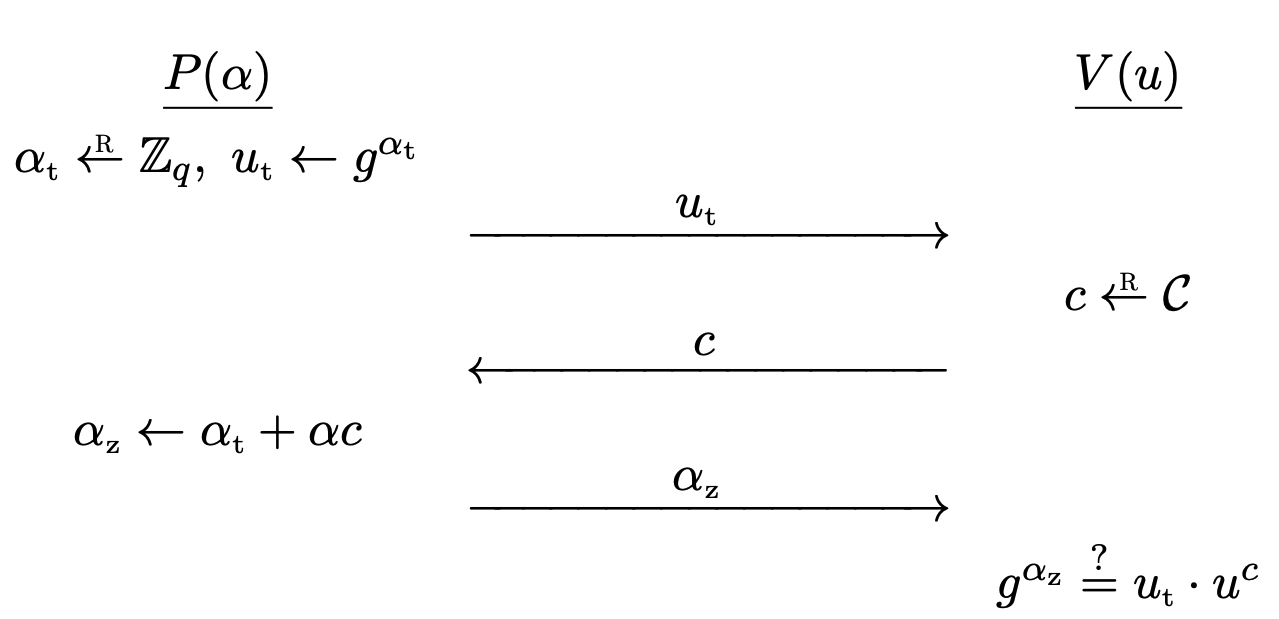
\includegraphics[width=0.55\linewidth]{figures/chapter19/fig1.png}
  \caption{Schnorr身份识别协议}
  \label{fig:19-1}
\end{figure}

$P(\alpha)$ 和 $V(u)$ 之间的一次交互产生一个\textbf{对话 (conversation)} $(u_{\rm t},c,\alpha_{\rm z})\in \mathbb{G}\times \mathcal{C}\times \mathbb{Z}_q$。如果 $V$ 的检查通过,即$g^{\alpha_{\rm z}}=u_{\rm t}\cdot u^c$ 成立,我们就称该对话为 \textbf{$u$ 的接受对话 (accepting conversation for $u$)}。不难看出,$P$ 和 $V$ 之间的交互总是能够产生一个接受对话,因为如果有 $u_{\rm t}=g^{\alpha_{\rm t}}$ 且 $\alpha_{\rm z}=\alpha_{\rm t}+\alpha c$,则有:
$$g^{\alpha_{\rm z}}=g^{\alpha_{\rm t}+\alpha c}=g^{\alpha_{\rm t}}\cdot (g^\alpha)^c=u_{\rm t}\cdot u^c$$
因此,Schnorr 协议能够满足身份识别协议所必需的基本正确性要求。

我们称集合 $\mathcal{C}$ 为\textbf{挑战空间 (challenge space)}。为了满足安全需求,我们要求 $|\mathcal{C}|$ 是超多项式的。事实上我们可以简单地取 $\mathcal{C}$ 为 $\mathbb{Z}_q$,但是技术上也可以允许更小的挑战空间。尽管我们最终会证明Schnorr协议在DL假设下对窃听攻击是安全的,但我们现在先从一个更简单的定理开始,它只证明了Schnorr协议对\emph{直接}攻击的安全性(攻击游戏 \ref{game:18-1})。

在证明这一点时,我们将表明,任何能够以不可忽略的概率成功执行直接仿冒攻击的对手,都能被转换成一个从验证密钥 $u$ 中高效地恢复私钥 $\alpha$的算法。由于这个原因,Schnorr的协议有时也被称为离散对数的知识证明。

\begin{theorem}\label{theo:19-1}
	基于 $\mathbb{G}$ 上的离散对数假设,假设 $N:=|\mathcal{C}|$ 是超多项式的,Schnorr 身份认证协议对直接攻击是安全的。
	\begin{quote}
		特别地,假设 $\mathcal{A}$ 是一个有效冒充对手,它通过攻击游戏 \ref{game:18-1} 中的直接攻击方式攻击 $\mathcal{I}_{\rm sch}$ 的优势为 $\epsilon:={\rm ID1\mathsf{adv}}[\mathcal{A},\mathcal{I}_{\rm sch}]$。那么必然存在一个有效的离散对数对手 $\mathcal{B}$,其运行时间大致是 $\mathcal{A}$ 的两倍,其优势为 $\epsilon':={\rm DL\mathsf{adv}}[\mathcal{B},\mathbb{G}]$,并且有:
	\end{quote}
	\begin{equation}\label{eq:19-1}
		\epsilon'\geq \epsilon^2-\frac{\epsilon}{N}
	\end{equation}
	\begin{quote}
		也即:
	\end{quote}
	\begin{equation}\label{eq:19-2}
		\epsilon\leq\frac{1}{N}+\sqrt{\epsilon'}
	\end{equation}
\end{theorem}

\begin{proof}[证明思路]
假设攻击游戏 \ref{game:18-1} 中的对手 $\mathcal{A}$ 在攻击 $\mathcal{I}_{\rm sch}$ 时有优势 $\epsilon$。在该游戏中,挑战者生成验证密钥 $u=g^\alpha$。在对手 $\mathcal{A}$ 的冒充尝试中,它基于某个任意的对手策略生成了协议的第一条交互信息 $u_{\rm t}$。为了赢得游戏,对手 $\mathcal{A}$ 必须用一个有效应答 $\alpha_{\rm z}$ 来响应随机挑战 $c\in\mathcal{C}$,使得 $g^{\alpha_{\rm z}}=u_{\rm t}\cdot u^c$。直观地讲,如果 $\mathcal{A}$ 能以概率 $\epsilon$ 对一个这样的随机挑战产生一个有效应答,那么它就应该能以概率 $\epsilon^2$ 对\emph{两个}随机挑战产生一个有效的应答。要使这一直觉变得严谨,需要一个有点技术性的论证,我们将在随后的引理中给出。

下面,我们先介绍如何使用 $\mathcal{A}$ 计算随机数 $u\in\mathbb{G}$ 的离散对数。我们使用 $u$ 作为 $\mathcal{I}_{\rm sch}$ 的验证密钥,并让 $\mathcal{A}$ 生成协议的第一条交互 $u_{\rm t}$。然后我们向 $\mathcal{A}$ 提供一个随机挑战 $c$,并希望 $\mathcal{A}$ 产生一个有效应答 $\alpha_{\rm z}$。如果这确实发生了,我们就将 $\mathcal{A}$ 的内部状态``回溯"到它刚刚生成 $u_{\rm t}$ 后的那一刻,然后给 $\mathcal{A}$ 提供另一个随机挑战 $c'$,并希望 $\mathcal{A}$ 产生另一个有效应答 $\alpha_{\rm z}'$。

如果上面这些都发生了,那么对于一个给定的验证密钥 $u$,我们就得到了两个接受对话 $(u_{\rm t},c,\alpha_{\rm z})$ 和 $(u_{\rm t},c',\alpha_{\rm z}')$,且这两个对话的第一条交互 $u_{\rm t}$ 相同。此外,由于 $\mathcal{C}$ 是超多项式的,因此我们可以以压倒性的概率得到 $c'\neq c$ 。基于以上信息,我们可以很容易地计算出 ${\rm \mathsf{Dlog}}_gu$。事实上,由于上面的两个对话都是接受对话,我们有下面两个等式:
$$g^{\alpha_{\rm z}}=u_{\rm t}\cdot u^c,~~~~
g^{\alpha_{\rm z}'} =u_{\rm t}\cdot u^{c'}$$
用第一式除以第二式, $u_{\rm t}$ 就被抵消了,于是我们有:
\begin{equation}\label{eq:19-3}
	g^{\Delta\alpha}=u^{\Delta c}
\end{equation}
其中$\Delta\alpha:=\alpha_{\rm z}-\alpha_{\rm z}'$,$\Delta c:=c-c'$。由于 $\Delta c\neq 0$,且循环群 $\mathbb{G}$ 的阶 $q$ 是素数,所以倒数 ${1}/{\Delta c}$ 存在于 $\mathbb{Z}_q$ 中。我们可以将式 \ref{eq:19-3} 中等式的左右两边都升阶 ${1}/{\Delta c}$,于是有:
	$$g^{{\Delta\alpha}/{\Delta c}}=u$$
因此,我们可以有效计算离散对数 ${\rm \mathsf{Dlog}}_gu$,其值为 ${\Delta\alpha}/{\Delta c}$。

读者应该注意到,这里提出的从两个接受对话中提取离散对数的技术,与事实 10.3 中使用的想法基本相同。事实上,使用 10.6.1 节中的术语,我们可以看到 $(\alpha_{\rm z},-c)$ 和 $(\alpha_{\rm z}',-c')$ 是 $u_{\rm t}$ 相对于$g$ 和 $u$ 的不同表示。事实 10.3 告诉了我们如何从这两个表示中计算出 ${\rm \mathsf{Dlog}}_gu$。
\end{proof}

这个定理与我们在本文中迄今为止所介绍的所有其他安全定理有着质的不同。事实上,在这个定理的证明中,虽然我们表明每个攻击 $\mathcal{I}_{\rm sch}$ 的对手 $\mathcal{A}$ 都可以转化为破解离散对数问题的对手 $\mathcal{B}$,但我们构造的对手 $\mathcal{B}$ \emph{并不是} $\mathcal{A}$ 的基本包装器,因为对手 $\mathcal{B}$ 要运行 $\mathcal{A}$ \emph{两次}。此外,这个定理在量上也是不同的,因为安全归约根本就不是很严密:如果 $\mathcal{A}$ 以概率 $\epsilon$ 获胜,那么 $\mathcal{B}$ 只能保证以 $\approx\epsilon^2$ 的概率获胜。

因此,为了使上述想法更严谨,我们需要先引入下面的引理:

\begin{lemma}[回溯引理]\label{theo:19-2}
	令 $S$ 和 $T$ 是两个非空有限集,$f:S\times T\to\{0,1\}$ 是一个函数。令 $\mathsf{X}$、$\mathsf{Y}$ 和 $\mathsf{Y}'$ 是相互独立的随机变量,其中 $\mathsf{X}$ 在集合 $S$ 中取值,$\mathsf{Y}$ 和 $\mathsf{Y}'$ 都在 $T$ 上均匀分布。令 $\epsilon:=\Pr[f(\mathsf{X},\mathsf{Y})=1]$,$N:=|T|$,则有:
	$$\Pr[f(\mathsf{X},\mathsf{Y})=1\land f(\mathsf{X},\mathsf{Y}')=1\land \mathsf{Y}\neq\mathsf{Y}']\geq\epsilon^2-\frac{\epsilon}{N}$$
\end{lemma}

\begin{proof}
	对于每个 $s\in S$,令 $g(s):=\Pr[f(s,\mathsf{Y})=1]$。首先,我们可以观察到 $E[g(\mathsf{X})]=\epsilon$,这是因为:
	\begin{equation*}
		\begin{aligned}
			E[g(\mathsf{X})]
			&=\sum_{s\in S}g(s)\Pr[\mathsf{X}=s]=\sum_{s\in S}\Pr[f(s,\mathsf{Y})=1]\Pr[\mathsf{X}=s]\\
			&=\sum_{s\in S}\Pr[f(s,\mathsf{Y})=1\land \mathsf{X}=s] \text{ \emph{(独立性)}}\\
			&=\sum_{s\in S}\Pr[f(\mathsf{X},\mathsf{Y})=1\land \mathsf{X}=s]\\
			&=\Pr[f(\mathsf{X},\mathsf{Y})=1] \text{ \emph{(全概率)}}\\
			&=\epsilon
		\end{aligned}
	\end{equation*}
	
	其次,考虑一个固定的 $s∈S$,令 $\mathcal{U}_s$ 为 $f(s,\mathsf{Y})=1\land f(s,\mathsf{Y}')=1\land \mathsf{Y}\neq\mathsf{Y}'$ 成立的事件,我们称:
	$$
	\Pr[\mathcal{U}_s]=g(s)^2-\frac{g(s)}{N}
	$$
	为了证明这一点,令 $N_s$ 是满足 $f(s, t)=1$ 的 $t\in T$ 的数量,那么有 $N_s$ 种方法可以选择满足 $f(s,\mathsf{Y})=1$ 的 $\mathsf{Y}$。而对于每个 $\mathsf{Y}$ 的选择,有 $N_s-1$ 种方法可以选择满足 $f(s,\mathsf{Y}')=1\land \mathsf{Y}\neq\mathsf{Y}'$ 的 $\mathsf{Y}'$。由于 $g(s)={N_s}/{N}$,因此我们有:
	$$
	\Pr[\mathcal{U}_s]=\frac{N_s(N_s-1)}{N^2}=\frac{N_s^2}{N^2}-\frac{N_s}{N^2}=g(s)^2-\frac{g(s)}{N}
	$$

	最后,令 $\mathcal{U}$ 为 $f(\mathsf{X},\mathsf{Y})=1\land f(\mathsf{X},\mathsf{Y}')=1\land \mathsf{Y}\neq\mathsf{Y}'$ 成立的事件,我们有:
	\begin{equation*}
		\begin{aligned}
			\Pr[\mathcal{U}]
			&=\sum_{s\in S}\Pr[\mathcal{U}\land\mathsf{X}=s]\text{ \emph{(全概率)}}\\
			&=\sum_{s\in S}\Pr[f(s,\mathsf{Y})=1\land f(s,\mathsf{Y}')=1\land \mathsf{Y}\neq\mathsf{Y}'\land\mathsf{X}=s]\\
			&=\sum_{s\in S}\Pr[f(s,\mathsf{Y})=1\land f(s,\mathsf{Y}')=1\land \mathsf{Y}\neq\mathsf{Y}']\cdot\Pr[\mathsf{X}=s]\text{ \emph{(独立性)}}\\
			&=\sum_{s\in S}\Pr[\mathcal{U}_s]\cdot\Pr[\mathsf{X}=s]=\sum_{s\in S}[g(s)^2-\frac{g(s)}{N}]\cdot\Pr[\mathsf{X}=s]\\
			&=E[g(\mathsf{X})^2]-\frac{g(\mathsf{X})}{N}\\
			&\geq E[g(\mathsf{X})]^2-\frac{E[g(s)]}{N}=\epsilon^2-\frac{\epsilon}{N}
		\end{aligned}
	\end{equation*}
	上面我们使用了这样一个一般事实:对于任意随机变量 $\mathsf{Z}$ 都有 $E[\mathsf{Z}^2]\geq E[\mathsf{Z}]^2$,在这里我们的这个 $\mathsf{Z}=g(\mathsf{X})$。这是詹森不等式的一个特例。
\end{proof}

\begin{proof}[定理 \ref{theo:19-1} 的证明]
	利用具有优势 $\epsilon$ 的冒充对手 $\mathcal{A}$ ,我们能够建立一个具有优势 $\epsilon'$ 的 DL 对手 $\mathcal{B}$,如下所示。对手 $\mathcal{B}$ 从其挑战者那里得到一个 DL 问题实例 $u = g^\alpha$,而我们的目标是让 $\mathcal{B}$ 在 $\mathcal{A}$ 的帮助下计算出 $\alpha$。$\mathcal{B}$ 的计算过程可以分为两个阶段。

在第一阶段,$\mathcal{B}$ 扮演 $\mathcal{A}$ 的挑战者的角色,将 $u$ 的值交给 $\mathcal{A}$ 作为验证公钥。在这一步中,$\mathcal{B}$ 的目标是计算出两个具有不同挑战的 $u$ 的接受对话,即:
$$(u_{\rm t},c,\alpha_{\rm z}),~~(u_{\rm t},c',\alpha_{\rm z}')$$
其中:
$$g^{\alpha_{\rm z}}=u_{\rm t}\cdot u^c,~~
g^{\alpha_{\rm z}'}=u_{\rm t}\cdot u^{c'},~~
c\neq c'$$

以下是 $\mathcal{B}$ 做到这一点的方法:
\begin{enumerate}
	\item $\mathcal{A}$ 扮演证明者,并将 $u_{\rm t}$ 发送给扮演验证者的 $\mathcal{B}$;
	\item $\mathcal{B}$ 向 $\mathcal{A}$ 发送一个随机数 $c\in\mathcal{C}$;
	\item $\mathcal{A}$ 向 $\mathcal{B}$ 发送 $\alpha_{\rm z}$;
	\item $\mathcal{B}$ 对 $\mathcal{A}$ 进行``回溯"操作,使 $\mathcal{A}$ 的内部状态与步骤 1 结束时完全相同,然后 $\mathcal{B}$ 向 $\mathcal{A}$ 发送一个新的随机数 $c'\in\mathcal{C}$;
	\item $\mathcal{A}$ 向 $\mathcal{B}$ 发送 $\alpha_{\rm z}'$。
\end{enumerate}
下面我们应用回溯引理 \ref{theo:19-2}。在该引理中,随机变量 $\mathsf{Y}$ 与挑战 $c$ 对应,$\mathsf{Y}'$ 与挑战 $c'$ 对应,$\mathsf{X}$ 与 $\mathcal{A}$ 、$\mathcal{B}$ 和 $\mathcal{B}$ 的挑战者的所有其他随机选择对应,具体包括群 $\mathbb{G}$ 和群元素 $g,u,u_t\in\mathbb{G}$。当产生的对话是 $u$ 的一个接受对话时,引理中的函数 $f$ 为 $1$,否则就为 $0$。因此,如果 $(u_{\rm t},c,\alpha_{\rm z})$ 是 $u$ 的接受对话,则 $f(\mathsf{X},\mathsf{Y})=1$,如果 $(u_{\rm t},c',\alpha_{\rm z}')$ 是 $u$ 的接受性对话,则 $f(\mathsf{X},\mathsf{Y}')=1$。应用该引理,我们发现 $\mathcal{B}$ 得到两个不同挑战的接受对话的概率至少为 $\epsilon^2-{\epsilon}/{N}$。

所以现在假设 $\mathcal{B}$ 已经成功计算出两个这样的接受对话 $(u_{\rm t},c,\alpha_{\rm z})$ 和 $(u_{\rm t},c',\alpha_{\rm z}')$。在第二阶段,$\mathcal{B}$ 用这两个对话来计算 $\alpha$。事实上,正如在上面的证明思路中已经讨论过的,我们可以计算$\alpha={\Delta\alpha}/{\Delta c}$,其中$\Delta\alpha:=\alpha_z-\alpha_z'$,$\Delta c:=c-c'$。

这就得到了式 \ref{eq:19-1}。下面我们论证式 \ref{eq:19-2} 可由式 \ref{eq:19-1} 推出。为此,我们不妨假设 $\epsilon\geq{1}/{N}$,否则式 \ref{eq:19-2} 显然是成立的。因此我们有:
$$
\begin{aligned}
	(\epsilon-\frac{1}{N})^2
	&=\epsilon^2-\frac{2\epsilon}{N}+\frac{1}{N^2}\leq\epsilon^2-\frac{2\epsilon}{N}+\frac{\epsilon}{N} \text{\emph{ (因为 }}\epsilon\geq\frac{1}{N}\text{\,)}\\
	&=\epsilon^2-\frac{\epsilon}{N}\leq \epsilon' \text{ \emph{(式}\ref{eq:19-1} \emph{)}}
\end{aligned}
$$
因此式 \ref{eq:19-2} 得证。

回顾一下,我们展示了如何从恶意验证者 $\mathcal{A}$ 中有效地\emph{提取}私钥 $\alpha$,进而证明了针对直接攻击的安全性。这使我们能够利用恶意验证者来解决$\mathbb{G}$中的离散对数问题。我们的\emph{提取器}通过回溯证明者的状态来获得两个接受对话 $(u_{\rm t},c,\alpha_{\rm z})$ 和 $(u_{\rm t},c',\alpha_{\rm z}')$,其中 $c\neq c'$。在安全性证明中回溯证明者 $\mathcal{A}$ 是可能的,因为我们完全控制了 $\mathcal{A}$ 的执行环境。在现实世界中,由于不能对诚实证明 $P$ 进行回溯,攻击者就不能使用这种策略从 $P$ 那里提取私钥。
\end{proof}

\subsection{诚实验证者零知识和针对窃听的安全性}\label{subsec:19-1-1}

我们已经证明了在离散对数假设下,Schnorr 协议对\emph{直接}攻击是安全的。事实上在相同的假设下,Schnorr 协议对于\emph{窃听}攻击也是安全的。现在,在某次窃听攻击中,对手获得了 $vk$ 和一张记录列表,该表的内容是$P$(在输入$sk$上)与 $V$(在输入$vk$上)之间的若干对话。我们的想法是证明这些对话对于对手来说没有任何帮助,因为在给定 $vk$ 而没有给定 $sk$ 的情况下,对手也可以自己有效地生成这些对话。如果我们能证明这一点,我们也就大功告成了。事实上,假设 $\mathcal{A}$ 是一个对手,它通过窃听成功发动仿冒攻击的优势是不可忽略不计的。然后,我们用另一个对手 $\mathcal{B}$ 来替代 $\mathcal{A}$,它的工作方式与 $\mathcal{A}$ 是一样的,只是现在 $\mathcal{B}$ 自己生成了对话列表,而不是从挑战者那里获取记录。这样,$\mathcal{B}$ 就发动了一个直接攻击,但是它与发动仿冒攻击的 $\mathcal{A}$ 具有相同的优势。

下面,我们将上面的想法扩展到更一般的情况,引入\textbf{诚实验证者零知识} 的概念。

\begin{definition}
	令 $\mathcal{I}=(G,P,V)$ 是一个身份识别协议。如果存在一个有效的概率性算法 $Sim$(称为\textbf{模拟器 simulator})使得对于 $G$ 的任意可能输出 $(vk,sk)$,$Sim$ 在输入 $vk$ 上的输出分布与 $P$ (在输入$sk$上)与 $V$(在输入$vk$上) 之间对话记录的分布相同,我们就称 $\mathcal{I}$ 是\textbf{诚实验证者零知识 (honest verifier zero knowledge, HVZK)} 的。
\end{definition}

下面,我们对其中的一些术语进行说明。所谓``零知识"的意思是,对手从 $P$ 那里什么也学不到,因为对手可以在不知道 $sk$ 的情况下自己使用算法 $Sim$ 模拟对话。而``诚实验证者"表达了这样一个事实,即这种模拟只对 $P$ 和\emph{诚实的}验证者 $V$ 之间的对话有效,而对于\emph{非诚实}的验证者,比如\emph{主动}攻击中可能出现的验证者,都是无效的。零知识的概念,包括诚实验证者零知识以及许多其他的变体,还会出现在身份识别协议之外的许多其他类型的协议中。

\begin{theorem}\label{theo:19-3}
	如果一个身份识别协议 $\mathcal{I}=(G,P,V)$ 对于直接攻击是安全的,且该协议是 HVZK 的,那么该协议对于窃听攻击也是安全的。
	\begin{quote}
		特别地,如果 $\mathcal{I}$ 是带有模拟器 ${Sim}$ 的 HVZK,那么对于每一个通过攻击游戏 18.2 中的窃听攻击来攻击 $\mathcal{I}$ 的冒充对手 $\mathcal{A}$,如果 $\mathcal{A}$ 最多能获得 $Q$ 次交互记录,必然存在一个通过攻击游戏 \ref{game:18-1} 中的直接攻击来攻击 $\mathcal{I}$ 的对手 $\mathcal{B}$,其中 $\mathcal{B}$ 是 $\mathcal{A}$ 的一个基本包装器,并且 $\mathcal{B}$ 最多运行 $Q$ 次 ${Sim}$,使得:
		$${\rm ID2\mathsf{adv}}[\mathcal{A},\mathcal{I}]=
			{\rm ID1\mathsf{adv}}[\mathcal{B},\mathcal{I}]$$
	\end{quote}
\end{theorem}

\begin{proof}
	$\mathcal{B}$ 的工作方式与 $\mathcal{A}$ 相同,只是它不是从挑战者那里获得交互记录,而是用 ${Sim}$ 自己生成交互记录。对手 $\mathcal{B}$ 的工作方式如图 \ref{fig:19-2} 所示。
\end{proof}

\begin{figure}
  \centering
  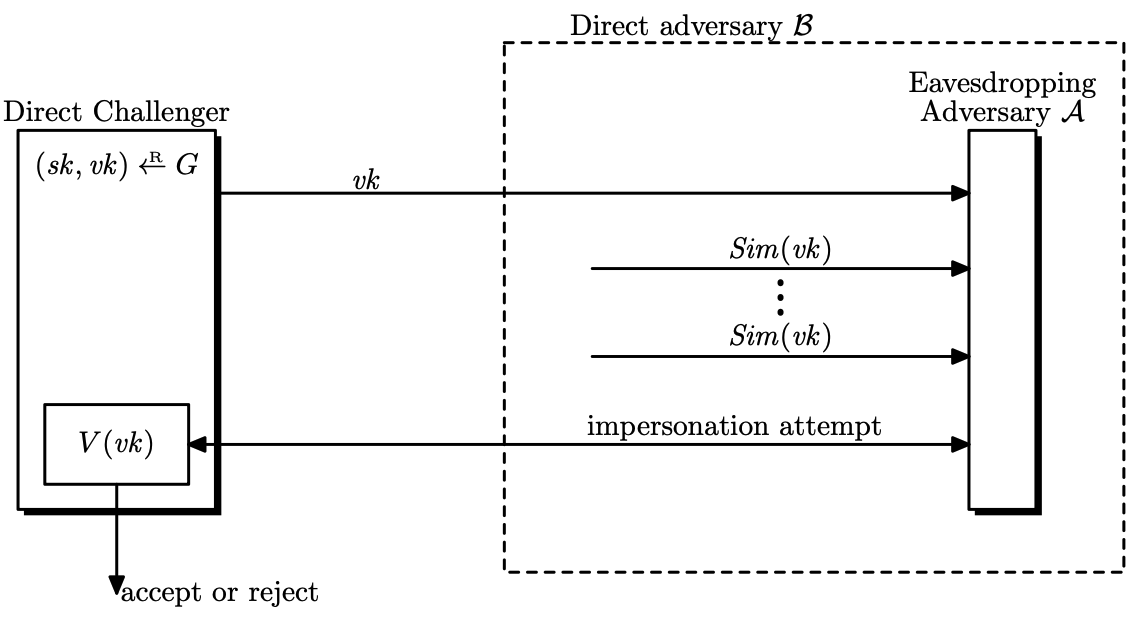
\includegraphics[width=0.65\linewidth]{figures/chapter19/fig2.png}
  \caption{定理 \ref{theo:19-3} 的证明中的对手 $\mathcal{B}$}
  \label{fig:19-2}
\end{figure}

下面让我们回到 Schnorr 身份识别协议。

\begin{theorem}\label{theo:19-4}
	Schnorr 身份识别协议是 HVZK 的。
\end{theorem}

\begin{proof}
	证明的思路是在生成模拟对话 $(u_{\rm t},c,\alpha_{\rm z})$ 时,我们不需要像 $P$ 和 $V$ 之间的真实对话那样,按照给定的顺序生成对话中的消息。事实上,模拟器 ${Sim}$ 是以\emph{倒序}生成信息的。在输入 $vk=u$ 时,模拟器 ${Sim}$ 计算:
		$$\alpha_{\rm z}\overset{\rm R}\leftarrow\mathbb{Z}_q,~~
		c\overset{\rm R}\leftarrow\mathcal{C},~~
		u_{\rm t}\leftarrow\frac{g^{\alpha_{\rm z}}}{u^c}$$
	并输出对话 $(u_{\rm t},c,\alpha_{\rm z})$。
	
	现在我们论证 ${Sim}$ 在输入 $vk=u$ 上的输出具有正确的分布。一个关键性的观察是,在真实交互中,$c$ 和 $\alpha_{\rm z}$ 是相互独立的,$c$ 在 $\mathcal{C}$ 上均匀分布,而 $\alpha_z$ 在 $\mathbb{Z}_q$ 上均匀分布。此外,给定 $c$ 和 $\alpha_{\rm z}$,$u_{\rm t}$ 的值可由等式 $g^{\alpha_{\rm z}}=u_{\rm t}\cdot u^c$ 唯一确定。而这显然与模拟器的输出分布相同。
\end{proof}

作为一个推论,我们立即可以得到:

\begin{theorem}\label{theo:19-5}
	如果 Schnorr 身份识别协议对直接攻击是安全的,那么它对窃听攻击也是安全的。
	
	\begin{quote}
		特别地,对于每个通过攻击游戏 18.2 中的窃听攻击来攻击 $\mathcal{I}_{\rm sch}$ 的冒充对手 $\mathcal{A}$,都有一个通过攻击游戏 \ref{game:18-1} 中的直接攻击来攻击 $\mathcal{I}_{\rm sch}$ 的对手 $\mathcal{B}$,其中 $\mathcal{B}$ 是 $\mathcal{A}$ 的一个基本包装器,满足:
		$${\rm ID2\mathsf{adv}}[\mathcal{A},\mathcal{I}_{\rm sch}]=
		{\rm ID1\mathsf{adv}}[\mathcal{B},\mathcal{I}_{\rm sch}]$$
	\end{quote}
\end{theorem}

乍看之下,我们关于 Schnorr 协议的结论似乎是反直觉的,甚至可能是矛盾的。在只知道 $vk$ 的情况下,怎么可能既很难进行冒充攻击,又容易产生对话呢?答案是,在进行冒充攻击时,验证者 $V$ 主动地参与对话,而消息的时间和顺序至关重要:扮演证明者的对手必须在看到 $V$ 生成的挑战 $c$ \emph{之前}生成第一条消息 $u_{\rm t}$。然而,模拟器可以自由地以任何方便的顺序生成信息:在定理 \ref{theo:19-4} 的证明中,模拟器先生成了 $c$ 和 $\alpha_{\rm z}$,然后才计算 $u_{\rm t}$。这些结果表明,如果挑战空间很小,Schnorr 协议将是完全\emph{不安全}的:在冒充尝试中,对手可以使用模拟器准备一个接受对话 $(u_{\rm t},c,\alpha_{\rm z})$,然后将 $u_{\rm t}$ 发送给 $V$,然后希望 $V$ 选择的挑战等于其准备的挑战 $c$。如果真的是这样,对手就可以用 $\alpha_{\rm z}$ 应答从而使 $V$ 接受对话。因此,以 ${1}/{|\mathcal{C}|}$ 的优势破解 Schnorr 识别协议是很容易的。所以为了确保安全性,挑战空间的大小 $|\mathcal{C}|$ 必须是超多项式的。

Schnorr 识别协议对攻击游戏 18.3 中的\emph{主动}攻击是否安全是一个开放的问题:目前还没有已知的有效主动攻击,但也没有证据可以排除离散对数假设下的这种攻击。在本章的稍后部分,我们将介绍一个对Schnorr身份识别的细小变化,它被证明在DL假设下对主动攻击是安全的。
\section{从身份识别协议到签名}\label{sec:19-2}

在本节中,我们将展示如何将 Schnorr 协议转换为一个签名方案。在离散对数假设下,该签名方案在随机预言机模型下是安全的。在本章的稍后部分,我们将看到这个构造实际上是一个更一般的结构的一个具体实例。

我们从 Schnorr 识别协议 $\mathcal{I}_{\rm sch}$ 开始,它定义在阶为素数 $q$ 的循环群 $\mathbb{G}$ 上,该群有生成元 $g\in\mathbb{G}$。此外,其挑战空间 $\mathcal{C}\subseteq\mathbb{Z}_q$。除此之外,我们还需要一个哈希函数 $H:\mathcal{M}\times\mathbb{G}\to\mathcal{C}$,该函数在安全证明中被建模为一个随机预言机。这里的 $\mathcal{M}$ 将会是签名方案的消息空间。

签名方案的构造思想是,对于消息 $m\in\mathcal{M}$ 的签名是一个元组 $(u_{\rm t},\alpha_{\rm z})$,其中 $(u_{\rm t},c,\alpha_{\rm z})$ 是在 Schnorr 识别协议 $\mathcal{I}_{\rm sch}$ 中对验证密钥 $u$ 的接受对话,挑战则来自 $c\leftarrow H(m,u_{\rm t})$。直观地讲,哈希函数 $H$ 在这里扮演 Schnorr 身份识别协议中验证者的角色。

具体地,Schnorr 签名方案为 $\mathcal{S}_{\rm sch}=(G,S,V)$,其中:
\begin{itemize}
	\item 密钥生成算法 $G$ 按如下方式运行:
	    \[
	    \alpha\overset{\rm R}\leftarrow\mathbb{Z}_q,
	    \quad
	    u\leftarrow g^\alpha
	    \]
	    其中公钥为 $pk:=u$,私钥为 $sk:=\alpha$。
	\item 为了使用私钥 $sk=\alpha$ 对消息 $m\in\mathcal{M}$ 进行签名,签名算法 $S$ 按如下方式运行:
		\[
		\alpha_{\rm t}\overset{\rm R}\leftarrow\mathbb{Z}_q,
		\quad	
		u_{\rm t}\leftarrow g^{\alpha_{\rm t}},
		\quad
		c\leftarrow H(m,u_{\rm t}),
		\quad
		\alpha_{\rm z}\leftarrow\alpha_{\rm t}+\alpha c
		\]
		输出签名 $\sigma:=(u_{\rm t},\alpha_{\rm z})$。
	\item 为了使用公钥 $pk=u$ 验证消息 $m\in\mathcal{M}$ 的签名 $\sigma=(u_{\rm t},\alpha_{\rm z})$,签名验证算法 $V$ 计算 $c\leftarrow H(m,u_{\rm t})$,当 $g^{\alpha_{\rm z}}=u_{\rm t}\cdot u^c$ 成立时输出 $\mathsf{accept}$,否则输出 $\mathsf{reject}$。
\end{itemize}

尽管我们把签名算法描述为一种随机化算法,但这并不是必须的。练习 \ref{exer:13-6} 展示了如何对签名算法进行去随机化。这种去随机化在实践中很重要,因为它可以避免不良随机性攻击,就像练习 \ref{exer:19-1} 所展示的那样。

我们下面将要说明,如果把 $H$ 建模为一个随机预言机,那么如果 Schnorr 识别协议对窃听攻击是安全的,那么 Schnorr 签名方案也一定是安全的。而我们已经在定理 \ref{theo:19-5} 中证明了前者。然而,首先考虑窃听攻击游戏的一个稍微增强的版本是有好处的。

\subsection{一个有用的抽象:重复冒充攻击}

我们考虑一种增强版本的针对识别协议的冒充攻击,在这种攻击中,我们允许对手反复进行冒充尝试,这些冒充尝试针对的是验证者的不同实例,它们同时运行,并使用相同的验证公钥。我们可以为直接攻击、窃听攻击和主动攻击定义这个概念,但我们目前先考虑窃听攻击,因为这就是我们的应用所需要的。另外,我们只考虑无状态和有验证公钥的识别协议。

下面是攻击游戏的更多细节。

\begin{game}[$r$ 次重复冒充窃听攻击]\label{game:19-1}
给定识别协议 $\mathcal{I}=(G,P,V)$,正整数 $r$ 和对手 $\mathcal{A}$,攻击游戏按以下流程运行。其密钥生成阶段和窃听阶段与攻击游戏 18.2 完全相同。

唯一不同的是冒充阶段。现在,我们允许对手 $\mathcal{A}$ 与最多 $r$ 个验证者同时互动。挑战者扮演这些验证者的角色,他们都使用在密钥生成阶段产生的相同的验证公钥。如果对手使这些验证者中的任何一个输出 $\mathsf{accept}$,我们就称它赢得了该游戏。

我们将 $\mathcal{A}$ 对于 $\mathcal{I}$ 和 $r$ 的优势记为 ${\rm rID2\mathsf{adv}}[\mathcal{A},\mathcal{I},r]$,其值等于 $\mathcal{A}$ 赢得该游戏的概率。
\end{game}

下面的引理将表明,$r$ 次重复冒充窃听攻击等价于普通的窃听攻击。也就是说,赢得攻击游戏 \ref{game:19-1} 并不会比赢得攻击游戏 18.2 更容易。

\begin{lemma}\label{theo:19-6}
令 $\mathcal{I}$ 是一个身份识别协议。对于每个 $r$ 次重复冒充窃听攻击对手 $\mathcal{A}$,都存在一个标准窃听对手 $\mathcal{B}$,其中 $\mathcal{B}$ 是一个围绕 $\mathcal{A}$ 的基本包装器,满足:

\begin{equation}
{\rm rID2\mathsf{adv}}[\mathcal{A},\mathcal{I},r]\leq r\cdot{\rm ID2\mathsf{adv}}[\mathcal{B}, \mathcal{I}]
\end{equation}

\end{lemma}

\begin{proof}[证明简述]
这是一个简单的“猜测论证”。对手 $\mathcal{B}$ 随机选择 $\omega\in\{1,\dots,r\}$,然后扮演 $\mathcal{A}$ 的挑战者。它首先从自己的挑战者那里获得验证公钥和几条对话记录,并将这些传递给 $\mathcal{A}$。在冒充阶段,对于验证者的第 $j$ 个实例,如果 $j\neq\omega$,对手 $\mathcal{B}$ 自己扮演验证者;否则,如果 $j=\omega$,对手 $\mathcal{B}$ 就作为 $\mathcal{A}$ 和攻击游戏 18.2 中它自己的挑战者之间的简单管道。显然,$\mathcal{A}$ 在与 $\mathcal{B}$ 游戏时让其中一个验证者输出 $\mathsf{accept}$ 的概率与攻击游戏 \ref{game:19-1} 中相同。此外,如果 $\mathcal{B}$ 猜到了其中一个输出 $\mathsf{accept}$ 的验证者的索引,它就赢得了攻击游戏,这发生的概率至少是 ${1}/{r}$。
\end{proof}

\subsection{Schnorr 签名的安全性分析}

我们下面将表明,只要 Schnorr 身份识别协议对窃听攻击是安全的,Schnorr 签名方案在随机预言机模型下就是安全的。

\begin{theorem}\label{theo:19-7}
如果 $H$ 是一个随机预言机,且 Schnorr 身份识别协议对窃听攻击是安全的,那么 Schnorr 签名方案也是安全的。

\begin{quote}
特别地,令 $\mathcal{A}$ 是如攻击游戏 13.1 的随机预言机模型那样攻击  $\mathcal{S}_{\rm sch}$ 的一个对手,假设 $\mathcal{A}$ 最多发起 $Q_{\rm s}$ 次签名查询和 $Q_{\rm ro}$ 次随机预言机查询。那么必然存在一个 $(Q_{\rm ro}+1)$ 次重复冒充攻击对手 $\mathcal{B}$ 能够通过攻击游戏 \ref{game:19-1} 中的窃听攻击来攻击  $\mathcal{I}_{\rm sch}$,其中 $\mathcal{B}$ 是一个围绕 $\mathcal{A}$ 的基本包装器,满足:
\end{quote}
\begin{equation}\label{eq:19-5}
{\rm SIG^{ro}\mathsf{adv}}[\mathcal{A}, \mathcal{S}_{\rm sch}]\leq{Q_{\rm s}(Q_{\rm s}+Q_{\rm ro}+1)}/{q}+{\rm rID2\mathsf{adv}}[\mathcal{B},\mathcal{I}_{\rm sch},Q_{\rm ro}+1]
\end{equation}
\end{theorem}

\begin{proof}[证明思路]
我们的目标是将伪造签名的对手 $\mathcal{A}$ 转化为在 $r$ 次重复冒充窃听攻击中破坏 Schnorr 身份识别协议安全性的对手 $\mathcal{B}$,其中 $r:=Q_{\rm ro}+1$。

第一个想法是,我们必须以某种方式在不使用私钥的情况下响应 $\mathcal{A}$ 的签名查询。想要实现这一点,可以通过利用窃听攻击中获取的对话记录来建立所需的签名,并``修正"随机预言机 $H$,使其与签名一致。只有当随机预言机在已经被查询过的位置重新被查询时,这种修复才会失败。但由于随机预言机的输入包括一个随机群元素,因此发生的概率极低。这也就是公式 \ref{eq:19-5} 中出现 ${Q_s(Q_s+Q_{\rm ro}+1)}/{q}$ 修正项的原因。

一旦摆脱了签名查询,我们认为,如果对手成功地伪造了签名,它就可以有效地被用于对  $\mathcal{I}_{\rm sch}$ 的 $r$ 次重复冒充窃听攻击。我们再次利用了 $H$ 被建模为一个随机预言机的事实。由于签名伪造必须被包含在没有被作为签名查询而提交的信息中,因此相应的随机预言机查询必须与所有签名查询的位置相异。由于伪造签名与签名查询不能同时作为同一条消息提交,因此相应的随机预言机查询必须与所有签名查询的位置相异。所以,该位置上随机预言机的输出值在身份识别协议的运行中基本上可以视作一个随机挑战。我们事先并不知道哪一个随机预言机查询对应于一个伪造签名,这就是我们必须使用 $r$ 次重复冒充窃听攻击游戏的原因。
\end{proof}

\begin{proof}
为了简化分析,我们将假设当 $\mathcal{A}$ 输出一个伪造签名 $(m,\sigma)$,$\sigma=(u_{\rm t},\alpha_{\rm z})$ 时,$\mathcal{A}$ 一定已经在 $(m,u_{\rm t})$ 这一点上显式地查询了随机预言机。如有必要,我们会修改 $\mathcal{A}$ 以确保这种情况,以使得修改后的 $\mathcal{A}$ 所进行的随机预言机查询次数最多为 $Q_{\rm ro}+1$。

我们下面将定义两个攻击游戏。游戏 0 基本上就是原始的签名攻击游戏,其中 $H$ 被建模为一个随机预言机。游戏 1 是一个少量修改后的版本。对于 $j=0,1$,我们记 $W_j$ 是 $\mathcal{A}$ 在游戏 $j$ 中获胜的事件。

\noindent
\textbf{游戏 0。}
挑战者的工作方式与攻击游戏 13.1 的随机预言机版本相同。与往常一样,我们用一个关联数组 $Map:\mathcal{M}\times\mathbb{G}\to\mathcal{C}$ 来实现随机预言机。我们还维护一个关联数组 $Explicit:\mathcal{M}\times\mathbb{G}\to\mathbb{Z}$ 以记录那些随机预言机第一次被对手显式查询的位置,而不包含被签名算法隐式地查询的位置。挑战者的工作逻辑如图 \ref{fig:19-3}。

\begin{figure}
  \hspace*{45pt} 初始化:\\
  \hspace*{70pt} 令 $\alpha\overset{\rm R}\leftarrow\mathbb{Z}_q$,计算 $u\leftarrow g^\alpha$\\
  \hspace*{70pt} 初始化两个空的关联数组 $Map:\mathcal{M}\times\mathbb{G}\to\mathcal{C}$ 和 $Explicit:\mathcal{M}\times\mathbb{G}\to\mathbb{Z}$\\
  \hspace*{70pt} 将公钥 $u$ 发送给 $\mathcal{A}$;\\
  \hspace*{45pt} 当收到第 $i$ 个签名查询 $m_i\in\mathcal{M}$ 时:\\
  \hspace*{70pt} 令 $\alpha_{{\rm t}i}\overset{\rm R}\leftarrow\mathbb{Z}_q$,$c_i\overset{\rm R}\leftarrow\mathcal{C}$,计算 $u_{{\rm t}i}\leftarrow g^{\alpha_{{\rm t}i}}$\\
  \hspace*{30pt} (1)
  \hspace*{43pt} 如果 $(m_i,u_{{\rm t}i})\in{\rm Domain}(Map)$,则令 $c_i\leftarrow Map[m_i,u_{{\rm t}i}]$\\
  \hspace*{70pt} 令 $Map[m_i,u_{{\rm t}i}]\leftarrow c_i$\\
  \hspace*{70pt} 计算 $\alpha_{{\rm z}i}\leftarrow\alpha_{{\rm t}i}+\alpha c_i$\\
  \hspace*{70pt} 将 $(u_{{\rm t}i},\alpha_{{\rm z}i})$ 发送给 $\mathcal{A}$;\\
  \hspace*{45pt} 当收到第 $j$ 个随机预言机查询 $(\hat m_j,\hat u_j)\in\mathcal{M}\times\mathbb{G}$ 时:\\
  \hspace*{70pt} 如果 $(\widehat m_j,\widehat u_j)\notin{\rm Domain}(Map)$:\\
  \hspace*{95pt} 令 $Map[\widehat m_j,\widehat u_j]\overset{\rm R}\leftarrow\mathcal{C}$,$Explicit[\widehat m_j,\widehat u_j]\leftarrow j$\\
  \hspace*{70pt} 将 $Map[\hat m_j,\hat u_j]$ 发送给 $\mathcal{A}$;\\
  \hspace*{45pt} 当收到一个伪造尝试 $(m,u_{\rm t},\alpha_{\rm z})$ 时:\\
  \hspace*{70pt} // \emph{根据假设,有 $(m,u_{\rm t})\in{\rm Domain}(Explicit)$}\\
  \hspace*{70pt} 如果 $g^{\alpha_{\rm z}}=u_{\rm t}\cdot u^c$,其中 $c=Map[m,u_{\rm t}]$:\\
  \hspace*{95pt} 则输出 ``win"\\
  \hspace*{95pt} 否则输出 ``lose"
  \caption{游戏0的挑战者}
  \label{fig:19-3}
\end{figure}

为了处理一个签名查询 $m_i$,挑战者像往常一样运行签名算法:它首先生成一个随机的 $\alpha_{{\rm t}i}\in\mathbb{Z}_q$ 并计算 $u_{{\rm t}i}\leftarrow g^{\alpha_{{\rm t}i}}$。然后它为 $Map[m_i,u_{{\rm t}i}]$ 的值生成一个随机``默认"值 $c_i\in\mathcal{C}$,如果通过行(1)的测试发现 $Map[m_i,u_{{\rm t}i}]$ 已经被定义,那么就使用那个先前定义的值,而不是默认值。

为了处理一个随机预言机查询 $(\widehat m_j,\widehat u_j)$,如果 $Map[\widehat m_j,\widehat u_j]$ 的值尚未被之前的签名查询或随机预言机查询所定义,就在此时定义它,并设定 $Explicit[\widehat m_j,\widehat u_j]\leftarrow j$。

假设对手提交一个伪造尝试 $(m,u_t,\alpha_{\rm z})$,且 $m$ 与作为签名查询提交的所有 $m_i$ 都不同,根据我们的简化假设,对手必须在之前曾将 $(m,u_{\rm t})$ 作为随机预言机查询提交,因此此时 $(m,u_{\rm t})$ 一定在 ${\rm Domain}(Explicit)$ 中。由此可见,如果 $(u_{\rm t},\alpha_{\rm z})$ 是一个有效签名,那么挑战者将输出 ``win",因此:
\[
{\rm SIG^{ro}\mathsf{adv}}[\mathcal{A}, \mathcal{S}_{\rm sch}]\leq\Pr[W_0]
\]

\noindent
\textbf{游戏 1。}
游戏 1 与游戏 0 基本相同,只是删去了图 \ref{fig:19-3} 中行(1)的测试。直接应用差分引理,我们就可以得到:
\[
|\Pr[W_1]-\Pr[W_0]|\leq\frac{Q_{\rm s}(Q_{\rm s}+Q_{\rm ro}+1)}{q}
\]
事实上,对于第 $i$ 个签名查询,$u_{{\rm t}i}$ 在 $\mathbb{G}$ 上均匀分布,联合约束意味着随机预言机已经在 $(m,u_{{\rm t}i})$ 位置上被查询过的概率最多是 ${Q_s(Q_s+Q_{\rm ro}+1)}/{q}$,查询既可能是对手发出的,也可能是之前的签名查询间接导致的。联合约束还意味着对于任何签名来说,发生该情况的概率的总上界为 ${Q_s(Q_s+Q_{\rm ro}+1)}/{q}$。

做出这一改变的意义在于,现在在游戏 1 中,一个新的随机挑战被用来处理每个签名查询,就像 Schnorr 身份识别协议中的诚实验证者一样。

基于此,很容易构建一个对手 $\mathcal{B}$,它对挑战者进行 $r=Q_{\rm ro}+1$ 的 $r$ 次重复冒充窃听攻击游戏,并且自己在游戏 1 中扮演 $\mathcal{A}$ 的挑战者的角色,因而:
\[
\Pr[W_1] = {\rm rID2\mathsf{adv}}[\mathcal{B},\mathcal{I}_{\rm sch},r]
\]
$\mathcal{B}$ 的工作逻辑如图 \ref{fig:19-4} 所示。对于 $j=1,\dots,r$,我们用 $V_j$ 表示在 $r$ 次重复冒充窃听攻击游戏中的第 $j$ 个验证者。这样定理 \ref{theo:19-7} 得证。
\end{proof}

\begin{figure}
  \hspace*{45pt} 初始化:\\
  \hspace*{70pt} 从挑战者处收到验证公钥 $u$\\
  \hspace*{70pt} 从挑战者处获取窃听对话 $(u_{{\rm t}i},c_i,\alpha_{{\rm z}i})$, $i=1,\dots,Q_s$\\
  \hspace*{70pt} 初始化两个空的关联数组 $Map:\mathcal{M}\times\mathbb{G}\to\mathcal{C}$ 和 $Explicit:\mathcal{M}\times\mathbb{G}\to\mathbb{Z}$\\
  \hspace*{70pt} 将 $u$ 发送给 $\mathcal{A}$;\\
  \hspace*{45pt} 当从 $\mathcal{A}$ 处收到第 $i$ 个签名查询 $m_i\in\mathcal{M}$ 时:\\
  \hspace*{70pt} 令 $Map[m_i,u_{{\rm t}i}]\leftarrow c_i$\\
  \hspace*{70pt} 将 $(u_{{\rm t}i},\alpha_{{\rm z}i})$ 发送给对手 $\mathcal{A}$;\\
  \hspace*{45pt} 当收到第 $j$ 个随机预言机查询 $(\widehat m_j,\widehat u_j)\in\mathcal{M}\times\mathbb{G}$ 时:\\
  \hspace*{70pt} 如果 $(\widehat m_j,\widehat u_j)\notin{\rm Domain}(Map)$:\\
  \hspace*{95pt} 发起对验证者 $V_j$ 的冒充尝试:\\
  \hspace*{120pt} 将 $\widehat u_j$ 发送给 $V_j$,后者将回复一个挑战 $\widehat c_j$\\
  \hspace*{95pt} 令 $Map[\widehat m_j,\widehat u_j]\leftarrow\widehat c_j$,$Explicit[\widehat m_j,\widehat u_j]\leftarrow j$\\
  \hspace*{70pt} 将 $Map[\widehat m_j,\widehat u_j]$ 发送给 $\mathcal{A}$;\\
  \hspace*{45pt} 当收到一个伪造尝试 $(m,u_{\rm t},\alpha_{\rm z})$ 时:\\
  \hspace*{70pt} // \emph{根据假设,有 $(m,u_{\rm t})\in{\rm Domain}(Explicit)$}\\
  \hspace*{70pt} 向 $V_j$ 发送最终消息 $\alpha_z$,其中 $j=Explicit[m,u_{\rm t}]$
  \caption{对手$\mathcal{B}$}
  \label{fig:19-4}
\end{figure}

\noindent
\textbf{将已有的结论结合起来。}
如果我们把定理 \ref{theo:19-7}、引理 \ref{theo:19-6}、定理 \ref{theo:19-5} 和定理 \ref{theo:19-1} 的结论结合起来,我们就可以得到下面的从对 Schnorr 签名方案的攻击到计算离散对数的问题归约。

\begin{quote}
\emph{令 $\mathcal{A}$ 是一个按照攻击游戏 13.1 中的随机预言机版本攻击 $\mathcal{S}_{\rm sch}$ 的有效对手。此外,假设 $\mathcal{A}$ 最多能发出 $Q_s$ 次签名查询和 $Q_{\rm ro}$ 次随机预言机查询。那么必然存在一个有效离散对数对手 $\mathcal{B}$,其运行时间大约是 $\mathcal{A}$ 的两倍,满足:}
\end{quote}
\begin{equation}\label{eq:19-6}
{\rm SIG^{ro}\mathsf{adv}}[\mathcal{A},\mathcal{S}_{\rm sch}]\leq\frac{Q_s(Q_s+Q_{\rm ro}+1)}{q}+\frac{Q_{\rm ro}+1}{N}+(Q_{\rm ro}+1)\sqrt{{\rm DL\mathsf{adv}}[\mathcal{B},\mathbb{G}]}
\end{equation}
\begin{quote}
\emph{其中 $N$ 是挑战空间的大小。}
\end{quote}

这种归约并不是非常严格。将标量 $(Q_{\rm ro}+1)$ 直接与 $\sqrt{{\rm DL\mathsf{adv}}[\mathcal{B},\mathbb{G}]}$ 相乘是很有问题的。事实上可以得到一个更严格的归约,方法是用 $\sqrt{Q_{\rm ro}+1}$ 代替 $(Q_{\rm ro}+1)$,这显然要好得多。诀窍是把引理 \ref{theo:19-6} 中的``猜测阶段"和定理 \ref{theo:19-1} 中的``回溯阶段"结合起来,变成一个单一且直接的归约。

\begin{lemma}\label{theo:19-8}
考虑定义在群 $\mathbb{G}$ 上的 Schnorr 身份识别协议 $\mathcal{I}_{\rm sch}$,其中 $\mathbb{G}$ 的阶为素数 $q$,有生成元 $g\in\mathbb{G}$,其挑战空间 $\mathcal{C}$ 的大小为 $N$。对于每个优势为 $\epsilon:={\rm rID2\mathsf{adv}}[\mathcal{A},\mathcal{I}_{\rm sch},r]$ 的攻击 $\mathcal{I}_{\rm sch}$ 的有效 $r$ 次重复冒充窃听攻击对手 $\mathcal{A}$ ,必然存在一个有效离散对数对手 $\mathcal{B}$,其运行时间约为 $\mathcal{A}$ 的两倍,其优势为 $\epsilon':={\rm DL\mathsf{adv}}[\mathcal{B},\mathbb{G}]$,使得:
\begin{equation}\label{eq:19-7}
\epsilon'\geq\frac{\epsilon^2}{r}-\frac{\epsilon}{N}
\end{equation}
这意味着:
\begin{equation}\label{eq:19-8}
\epsilon\leq\frac{r}{N}+\sqrt{r\epsilon'}
\end{equation}
\end{lemma}

\begin{proof}
让我们首先回顾一下 $\mathcal{A}$ 的攻击游戏是如何进行的。首先,攻击游戏 \ref{game:19-1} 中的挑战者向 $\mathcal{A}$ 发送一个用于 Schnorr 身份识别协议的验证公钥 $u\in\mathbb{G}$。然后,挑战者向 $\mathcal{A}$ 发送了几份交互的对话记录。最后,$\mathcal{A}$ 进入冒充阶段,它试图让$r$个验证者中的至少一个输出$\mathsf{accept}$。更详细的过程是这样的。对于第 $j$ 次运行,其中 $j$ 不大于 $r$,对手 $\mathcal{A}$ 向挑战者发送 $u_{{\rm t}j}$,挑战者用随机挑战 $c_j\in\mathcal{C}$ 来应答。在收到所有挑战后,$\mathcal{A}$ 要么输出 $\mathsf{fail}$,要么输出一个数对 $(i,\alpha_{\rm z})$,使得 $(u_{{\rm t}i},c_i,\alpha_{\rm z})$ 是验证公钥 $u$ 的接受对话。在后一种情况下,我们称 $\mathcal{A}$ \emph{在验证者 $i$ 处成功}。注意到 $\mathcal{A}$ 的优势是 $\epsilon=\sum_{j=1}^r\epsilon_j$,其中 $\epsilon_j$ 是 $\mathcal{A}$ 在验证者 $j$ 处成功的概率。

请注意,我们上面的描述其实稍稍简化了对手 $\mathcal{A}$ 在冒充阶段的行为。然而,由于对手可以自己观察到对话是否被接受,所以这并不是一个真正的限制:任何对手都可以被置于上面所描述的形式中,而完全不改变其优势,也不会显著增加其运行时间。另外,在定理 \ref{theo:19-7} 的证明中构建的 $r$ 次重复冒充窃听攻击对手本质上已经是这种形式了。

我们下面描述我们的离散对数对手 $\mathcal{B}$,它被给予一个 $u\in\mathbb{G}$,任务是计算出 $\mathsf{Dlog}_gu$。像往常一样,$\mathcal{B}$ 扮演 $\mathcal{A}$ 的挑战者的角色。首先,$\mathcal{B}$ 将 $u$ 作为验证公钥发送给 $\mathcal{A}$。然后,$\mathcal{B}$ 使用定理 \ref{theo:19-4} 中的模拟器生成对话记录,并将这些记录交给 $\mathcal{A}$。最后,$\mathcal{B}$ 让 $\mathcal{A}$ 完成冒充阶段,并向 $\mathcal{A}$ 提供随机挑战 $c_1,\dots,c_r$。如果 $\mathcal{A}$ 输出一个数对 $(i,\alpha_{\rm z})$,使得 $(u_{{\rm t}i},c_i,\alpha_{\rm z})$ 是验证公钥 $u$ 的接受对话,那么 $\mathcal{B}$ 将 $\mathcal{A}$ 回溯到它向第 $i$ 个验证者提交 $u_{{\rm t}i}$ 的时刻。然后对手 $\mathcal{B}$ 用一个新的随机挑战 $c'\in\mathcal{C}$ 来替换挑战 $c_i$,然后让 $\mathcal{A}$ 继续使用与之前相同的挑战 $c_j$,$j=i+1,\dots,r$完成冒充阶段的剩余部分。如果 $\mathcal{A}$ 输出一个数对 $(i',\alpha_{\rm z}')$ 使得 $i'=i$ 且 $(u_{{\rm t}i},c',\alpha_{\rm z}')$ 是验证公钥 $u$ 的接受对话,并且 $c'\neq c$,那么 $\mathcal{B}$ 就可以使用这两个接受对话来计算 $\mathsf{Dlog}_gu$,就像定理 \ref{theo:19-1} 的证明中那样。在这种情况下,我们称 $\mathcal{B}$ \emph{在验证者 $i$ 处成功}。可以注意到 $\mathcal{B}$ 的优势是 $\epsilon'=\sum_{j=1}^r\epsilon_j'$,其中 $\epsilon_j'$ 是 $\mathcal{B}$ 在验证者 $j$ 处成功的概率。

剩下的工作就是证明式 \ref{eq:19-7},注意式 \ref{eq:19-8} 可以用与定理 \ref{theo:19-1} 的证明中几乎相同的方法从式 \ref{eq:19-7} 推出。

我们声称,对于 $j=1,\dots,r$,必有:
\begin{equation}\label{eq:19-9}
\epsilon_j'\geq\epsilon_j^2-\frac{\epsilon_j}{N}
\end{equation}
事实上,对于给定索引 $j$,上述不等式必然成立,这是回溯引理 \ref{theo:19-2} 已经证明了的,其中的 $\mathsf{Y}$ 对应于挑战 $c_j$,$\mathsf{Y}'$ 对应于挑战 $c'$,而 $\mathsf{X}$ 对应于 $\mathcal{A}$、$\mathcal{B}$ 和 $\mathcal{B}$ 的挑战者的所有其他随机选择。如果 $\mathcal{A}$ 在验证者 $j$ 处成功,则引理 19.2 中的函数 $f$ 就被定义为 $1$。因此,如果 $i=j$ 且 $(u_{{\rm t}j},c_j,\alpha_{\rm z})$ 是一个接受对话,就有 $f(\mathsf{X},\mathsf{Y})=1$。同样地,如果 $i'=j$ 且 $(u_{{\rm t}j},c',\alpha_{\rm z}')$ 是一个接受对话,就有 $f(\mathsf{X},\mathsf{Y}')=1$。

由式 \ref{eq:19-9},我们可以得到:
\[
\epsilon'
=\sum_{j=1}^r\epsilon_j'
\geq\sum_{j=1}^r\epsilon_j^2-\sum_{j=1}^r\frac{\epsilon_j}{N}
\geq\frac{\epsilon^2}{r}-\frac{\epsilon}{N}
\]
最后一个不等式基于这样一个事实:对于任意函数 $g:\{1,\dots,r\}\to\mathbb{R}$,必然有:
\[
r\sum_{j=1}^rg(j)^2\geq(\sum_{j=1}^rg(j))^2
\]
这个结论也是显然的。比如在概率论中,对于任意随机变量 $\mathsf{X}$,必有 $E[\mathsf{X}^2]\geq E[\mathsf{X}]^2$。特别地,如果令 $\mathsf{X}:=g(\mathsf{R})$,其中 $\mathsf{R}$ 是在 $\{1,\dots,r\}$ 上的均匀分布,就转化成了我们上面的场景。
\end{proof}

基于这个结论,我们可以把式 \ref{eq:19-6} 中的约束替换成:
\begin{equation}
{\rm SIG^{ro}\mathsf{adv}}[\mathcal{A},\mathcal{S}_{\rm sch}]\leq\frac{Q_{\rm s}(Q_{\rm s}+Q_{\rm ro}+1)}{q}+\frac{Q_{\rm ro}+1}{N}+\sqrt{(Q_{\rm ro}+1)\cdot{\rm DL\mathsf{adv}}[\mathcal{B},\mathbb{G}]}
\end{equation}


\subsection{一个具体实现与一种优化方法}\label{subsec:19-2-3}

我们可以将 $\mathbb{G}$ 看作是定义在有限域 $\mathbb{F}_p$ 上的椭圆曲线群 P256,其中 $p$ 是一个 $256$ 位素数,具体信息可以参见 15.3 节。使用 $128$ 位的挑战就足够了。在这种情况下,Schnorr 签名 $(u_{\rm t},\alpha_{\rm z})$ 中的每个组成部分都是 $256$ 位的,一个 Schnorr 签名总共约为 $512$ 位。

由于挑战的长度比群元素的编码长度要短得多,下面介绍的 Schnorr 签名优化方案可以获得更短的签名。回顾一下,我们之前将 $m$ 上的签名定义为 $(u_{\rm t},\alpha_{\rm z})$,满足:
\[
g^{\alpha_{\rm z}}=u_{\rm t}\cdot u^c
\]
其中 $c:=H(m,u_{\rm t})$。现在,与之前不同,我们可以把签名定义为数对 $(c,\alpha_{\rm z})$,它满足:
\[
c=H(m,u_{\rm t})
\]
其中 $u_{\rm t}={g^{\alpha_{\rm z}}}/{u^c}$。变换 $(u_{\rm t},\alpha_{\rm z})\mapsto(H(m,u_{\rm t}),\alpha_{\rm z})$ 可以将一个常规的对 $m$ 的 Schnorr 签名映射到一个优化 Schnorr 签名上,而变换 $(c,\alpha_{\rm z})\mapsto({g^{\alpha_{\rm z}}}/{u^c},\alpha_{\rm z})$ 可以将一个优化 Schnorr 签名映射到一个常规 Schnorr 签名上。由此可见,伪造一个优化 Schnorr 签名等价于伪造一个常规 Schnorr 签名。进一步优化的话,我们还可以在公钥中存储 $u^{-1}$ 而不是 $u$,这将加快签名验证的速度。

通过上述参数的选择,我们可以将签名的长度从 $512$ 位减少到大约 $128+256=384$ 位,这大约减少 $25\%$ 的长度。
\section{案例研究:ECDSA签名}

1991 年,当需要制定数字签名的联邦标准时,美国国家标准研究所 (NIST) 考虑了一些可行的候选方案。由于 Schnorr 系统受专利保护,NIST 选择了一种基于 $\mathbb{Z}_p^*$ 的素阶子群的临时签名方案,该方案后来被称为\textbf{数字签名算法(Digital Signature Algorithm, DSA)}。该标准后来被更新以支持定义在有限域上的椭圆曲线群。由此产生的签名方案被称为 \textbf{ECDSA},后来被用在许多现实世界的系统中。我们下面会简要介绍 ECDSA 的工作原理,并讨论几个影响它安全性的问题。

ECDSA 签名方案 $(G,S,V)$ 使用有限域 $\mathbb{F}_p$ 上的椭圆曲线点群 $\mathbb{G}$。令 $g$ 是 $\mathbb{G}$ 的一个生成元,素数 $q$ 是群 $\mathbb{G}$ 的阶。我们还需要一个定义在 $(\mathcal{M},\mathbb{Z}_q^*)$ 上的哈希函数 $H$。该方案的工作原理如下:
\begin{itemize}
	\item $G()$:选择 $\alpha\overset{\rm R}\leftarrow\mathbb{Z}_q^*$,令 $u\leftarrow g^\alpha\in\mathbb{G}$。输出 $sk:=\alpha$,$pk:=u$。
	\item $S(sk,m)$:使用私钥 $sk=\alpha$ 签署消息 $m\in\mathcal{M}$:\\
		\hspace*{30pt} 重复:\\
		\hspace*{50pt} 选取 $\alpha_{\rm t}\overset{\rm R}\leftarrow\mathbb{Z}_q^*$,计算 $u_{\rm t}\leftarrow g^{\alpha_{\rm t}}$\\
		\hspace*{50pt} 令 $u_{\rm t}=(x,y)\in\mathbb{G}$,其中 $x,y\in\mathbb{F}_p$\\
		\hspace*{50pt} 将 $x$ 当作 $[0,p)$ 区间中的一个整数,令 $r\leftarrow[x]_q\in\mathbb{Z}_q$,即计算 $x$ 模 $q$\\
		\hspace*{50pt} 计算 $s\leftarrow\left({H(m)+r\alpha}\right)/{\alpha_t}\in\mathbb{Z}_q$\\
		\hspace*{30pt} 直至 $r\neq0$ 且 $s\neq0$\\
		\hspace*{30pt} 输出 $(r,s)$
	\item $V(pk,m,\sigma)$:使用公钥 $pk=u\in\mathbb{G}$ 验证对消息 $m\in\mathcal{M}$ 的签名 $\sigma=(r,s)\in(\mathbb{Z}_q^*)^2$:\\
		\hspace*{30pt} 计算 $a\leftarrow{H(m)}/{s}\in\mathbb{Z}_q$,$b\leftarrow{r}/{s}\in\mathbb{Z}_q$\\
		\hspace*{30pt} 计算 $\hat u_{\rm t}\leftarrow g^au^b\in\mathbb{G}$\\
		\hspace*{30pt} 令 $\hat u_{\rm t}=(\hat x,\hat y)\in\mathbb{G}$,其中 $\hat x,\hat y\in\mathbb{F}_p$\\
		\hspace*{30pt} 将 $\hat x$ 当作 $[0,p)$ 区间中的一个整数,令 $\hat r\leftarrow[\hat x]_q\in\mathbb{Z}_q$,即计算 $\hat x$ 模 $q$\\
		\hspace*{30pt} 如果 $r=\hat r$ 则输出 $\mathsf{accept}$,否则输出 $\mathsf{reject}$
\end{itemize}

当使用椭圆曲线 P256 时,$p$ 和 $q$ 都是 $256$ 位素数,因此一个 ECDSA 签名 $\sigma=(r,s)$ 的长度为 $512$ 位。

很容易说明该签名方案是正确的。对于 $G$ 输出的任意密钥对 $(pk,sk)$ 和任意消息 $m\in\mathbb{Z}_q$,如果 $\sigma\overset{\rm R}\leftarrow S(sk,m)$,那么 $V(pk,m,\sigma)$ 必然输出 $\mathsf{accept}$。原因是 $V$ 计算出的 $\hat u_{\rm t}$ 与 $S$ 计算出的 $u_{\rm t}$ 必然是相同的。

在特定强假设和理想的群 $\mathbb{G}$ 下 ECDSA 是安全的。

为了保证安全性,签名期间产生的随机值 $\alpha_{\rm t}$ 必须是新从 $\mathbb{Z}_q^*$ 中均匀挑选出的值。否则该方案会在强意义上变得不安全,因为攻击者可以得到签名私钥 $\alpha$。针对索尼 PlayStation 3 的攻击就曾经利用了这个漏洞,因为在该设计中,$\alpha_{\rm t}$ 对于所有发出的签名都是相同的。除此之外,一些针对比特币钱包的攻击也利用了这个问题,因为在一些硬件平台上生成质量较高的随机数是很困难的。一个常用的解决方案是修改签名算法,使得 $\alpha$ 是使用安全性高的 PRF 确定性地生成的,这种修改后的算法被称为\textbf{确定性 ECDSA}。Schnorr 签名协议也有同样的问题,因此这种优化也同样适用于它。

\begin{snote}[ECDSA不是强安全的.]
尽管 Schnorr 签名协议是强安全的(见练习 \ref{exer:19-15}),但 ECDSA 方案却不是。给定一个对消息 $m$ 的 ECDSA 签名 $\sigma=(r,s)$,任何人都可以对 $m$ 生成其他合法签名。比如说 $\sigma':=(r,-s)\in(\mathbb{Z}_q^*)^2$ 也是一个对消息 $m$ 的合法签名。这个 $\sigma'$ 之所以合法,是因为椭圆曲线上的点 $u_{\rm t}\in\mathbb{G}$ 的横坐标与另一点 ${1}/{u_{\rm t}}\in\mathbb{G}$ 的横坐标是相同的。
\end{snote}
\section{Sigma协议:基本定义}

Schnorr 协议是一类被称为 \textbf{Sigma 协议}的协议族的其中一个特例。在本节中,我们将介绍与 Sigma 协议相关的基本概念。随后我们将考察 Sigma 协议的一些实例及其应用:
\begin{itemize}
	\item 我们将考察如何使用 Sigma 协议来构建新的安全识别方案和签名方案;
	\item 我们将考察如何建立对于\emph{主动}攻击也能保证安全性的身份识别方案,即使这种方案不依赖于随机预言机启发法。回顾一下,我们之前介绍的 Schnorr 协议只能保证对窃听攻击的安全性;
	\item 在下一章,我们还将看到如何将 Sigma 协议应用于其他与身份识别和签名无关的应用。例如,我们将看到如何加密一条消息 $m$,然后向持怀疑态度的验证者``证明" $m$ 满足某些属性,而不向验证者透露关于 $m$ 的任何其他信息。
\end{itemize}


再回顾一下 Schnorr 识别协议。直观地说,该协议允许证明者 $P$ 说服持怀疑态度的验证者 $V$ 它知道一个满足某些关系的秘密,但不向 $V$ 透露任何关于该秘密的有用信息。对于 Schnorr 的协议,证明者的秘密是私钥 $\alpha\in\mathbb{Z}_q$,它满足关系 $g^\alpha=u$。

下面,我们尝试将其推广到更普遍也更有趣的关系类型。

\begin{definition}[有效关系]
一个\textbf{有效关系(effective relation)}是一个二元关系 $\mathcal{R}\subseteq\mathcal{X}×\mathcal{Y}$,其中 $\mathcal{X}$、$\mathcal{Y}$ 和 $\mathcal{R}$ 是可有效识别的有限集。$\mathcal{Y}$ 中的元素称为\textbf{陈述 (statements)}。如果 $(x,y)\in\mathcal{R}$,我们就称 \textbf{$x$ 是 $y$ 的见证(witness for $y$)}。
\end{definition}

下面,我们定义 Sigma 协议的语法。

\begin{definition}[Sigma 协议]
令 $\mathcal{R}\subseteq\mathcal{X}×\mathcal{Y}$ 是一个有效关系。一个 $\mathcal{R}$ 上的 \textbf{Sigma 协议}是一个对算法 $(P,V)$。
\begin{itemize}
	\item $P$ 是一个交互式协议算法,称为\textbf{证明者 (prover)},它接受一个见证-陈述对 $(x,y)\in\mathcal{R}$ 作为输入。
	\item $V$ 是一个交互式协议算法,称为\textbf{验证者 (verifier)},它接受一个陈述 $y\in\mathcal{Y}$ 作为输入,输出 $\mathsf{accept}$ 或 $\mathsf{reject}$。
	\item $P$ 和 $V$ 之间的交互按如下流程进行:
		\begin{itemize}
			\item 为了启动协议,$P$ 计算出一条消息 $t$,称为\textbf{承诺 (commitment)},并将 $t$ 发送给 $V$;
			\item 收到 $P$ 的承诺 $t$ 后,$V$ 从一个有限的\textbf{挑战空间 (challenge space)} $\mathcal{C}$ 中随机选取一个\textbf{挑战 (challenge)} $c$,并将 $c$ 发送给 $P$;
			\item 收到 $V$ 的挑战 $c$ 后,$P$ 计算出一个\textbf{应答 (response)} $z$,并将 $z$ 发送给 $V$;
			\item 收到 $P$ 的应答 $z$ 后,$V$ 输出 $\mathsf{accept}$ 或 $\mathsf{reject}$。$V$ 的输出必须严格作为陈述$y$和\textbf{对话(conversation)}$(t,c,z)$的函数。特别地,除了挑战 $c$ 的随机选择之外,$V$不做任何其他随机选择,即所有其他计算都是完全确定性的。
		\end{itemize}
\end{itemize}
我们要求,对于所有的 $(x,y)\in\mathcal{R}$,当 $P(x,y)$ 与 $V(y)$ 完成交互时,$V$ 总是会输出 $\mathsf{accept}$。
\end{definition}

\begin{figure}[hbt]
  \centering
  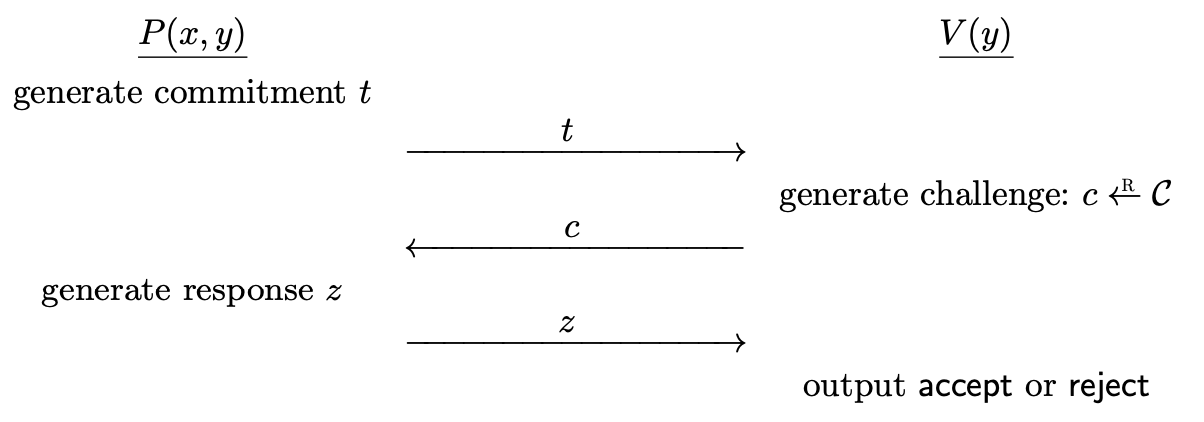
\includegraphics[width=0.75\linewidth]{figures/chapter19/fig5.png}
  \caption{Sigma协议的执行}
  \label{fig:19-5}
\end{figure}

图 \ref{fig:19-5} 展示了 Sigma 协议的执行流程。Sigma 协议的得名是因为这种协议中信息流的形状依稀让人想起希腊字母 $\Sigma$。

如定义所述,我们要求验证者的输出是陈述 $y$ 和对话 $(t,c,z)$ 的函数。当 $V$ 输出 $\mathsf{accept}$ 时,我们称对话 $(t,c,z)$ 是一个 $y$ \textbf{的接受对话 (accepting conversation for $y$)}。显然验证者与诚实的证明者之间只会产生接受对话;但当证明者不诚实或不遵循协议时,也有可能产生非接受对话。

在大多数 Sigma 协议的应用中,我们都会要求挑战空间的大小是超多项式的,为了简洁地表达该要求,我们有时也说协议需要\textbf{大的挑战空间}。

\begin{example}\label{exmp:19-1}
显然 Schnorr 识别协议 $(G,P,V)$ 中的算法 $(P,V)$ 是关系 $\mathcal{R}\subseteq\mathcal{X}×\mathcal{Y}$ 上的 Sigma 协议的一个特例,其中:
$$
\mathcal{X}=\mathbb{Z}_q,~~
\mathcal{Y}=\mathbb{G},~~
\mathcal{R}=\{(\alpha,u)\in\mathbb{Z}_q\times\mathbb{G}:g^\alpha=u\}
$$
挑战空间 $\mathcal{C}$ 是 $\mathbb{Z}_q$ 的一个子集。我们称 $(P,V)$ 为 \textbf{Schnorr的Sigma 协议 (Schnorr's Sigma protocol)}。

读者应该注意到,与识别协议不同的是,Sigma 协议本身并没有指定生成 $\mathcal{R}$ 中元素的算法。

还需要注意的是,关系 $\mathcal{R}$ 以群 $\mathbb{G}$ 作为参数,具体包括群 $\mathbb{G}$ 的阶 $q$ 和生成元 $g\in\mathbb{G}$。一般来说,我们允许用这种系统参数的方式来定义有效关系,这些参数在系统设置时产生,并公开给所有协议参与方。

Schnorr的Sigma 协议的陈述是一个群元素 $u\in\mathbb{G}$,而 $u$ 的见证是使得 $g^\alpha=u$ 成立的 $\alpha\in\mathbb{Z}_q$。因此每个陈述都对应着唯一的一个见证。一个 $u$ 的接受对话是一个形如 $(u_{\rm t},c,\alpha_{\rm z})$ 的三元组,其中 $u_{\rm t}\in\mathbb{G}$,$c\in\mathcal{C}$,$\alpha_{\rm z}\in\mathbb{Z}_q$,满足:
$$
g^{\alpha_{\rm z}}=u_{\rm t}\cdot u^c
$$

读者可能已经注意到,在 Schnorr 身份识别协议中,验证者 $P$ 只需要接受见证 $\alpha$ 作为输入,而不是像 Sigma 协议中所要求的见证-陈述对 $(\alpha,u)$。事实上,还有很多其他的 Sigma 协议的实例也同样不要求证明者在计算中显式地使用陈述。
\end{example}

\subsection{知识健全性}

接下来我们为 Sigma 协议定义一个关键的安全属性,称为\textbf{知识健全性 (knowledge soundness)}。

\begin{definition}[知识健全性]
令 $(P,V)$ 是一个关系 $\mathcal{R}\subseteq\mathcal{X}×\mathcal{Y}$ 上的 Sigma 协议,如果存在一个有效确定性算法 ${Ext}$(称为\textbf{见证提取器})具备下述属性:给定一个陈述 $y\in\mathcal{Y}$ 和 $y$ 的两个接受对话 $(t,c,z)$ 和 $(t,c',z')$ 作为输入,其中 $c\neq c'$,算法 ${Ext}$ 总是能输出 $x\in\mathcal{X}$ 使得 $(x,y)\in\mathcal{R}$,即 $x$ 是 $y$ 的一个见证;我们就称 Sigma 协议 $(P,V)$ 能够提供\textbf{知识健全性}。
\end{definition}

\begin{example}\label{exmp:19-2}
回顾例 \ref{exmp:19-1},我们很容易验证 Schnorr的Sigma 协议具备知识健全性。见证提取器 $\mathsf{Ext}$ 以 $u\in\mathbb{G}$ 为输入,并接受 $u$ 的两个接受对话 $(u_{\rm t},c,\alpha_{\rm z})$ 和 $(u_{\rm t},c',\alpha_{\rm z}')$,其中 $c\neq c'$。正如定理 \ref{theo:19-1} 的证明中所进行的操作,我们也可以从这两个接受对话中计算出相应的见证 $\alpha=\mathsf{Dlog}_gu$,其值为 ${\Delta\alpha}/{\Delta c}\in\mathbb{Z}_q$,其中 $\Delta\alpha:=\alpha_{\rm z}-\alpha_{\rm z}'$,$\Delta c:=c-c'$。
\end{example}

假设 $(P,V)$ 是关系 $\mathcal{R}\subseteq\mathcal{X}×\mathcal{Y}$ 上的 Sigma 协议。此外,假设 $(P,V)$ 提供知识健全性并且具有大的挑战空间。那么在某种意义上, $(P,V)$ 充当了一个\textbf{知识证明 (proof of knowledge)}。考虑任意一个证明者 $P^*$(甚至可能是一个潜在的``作弊"的验证者),使 $V$ 以不可忽略的概率接受一个陈述 $y$。那么$P^*$一定``知道" $y$ 的一个见证,方法如下:如定理 \ref{theo:19-1} 的证明中那样,我们可以回溯 $P^*$ 来得到 $y$ 的两个接受对话 $(t,c,z)$ 和 $(t,c',z')$,其中$c\neq c'$,然后使用见证提取器计算出见证 $x$。

更一般地说,当一个密码学家说 $P^*$ 一定``知道"一个陈述 $y$ 的见证时,她的意思是可以通过回溯从 $P^*$ 中提取出见证 $x$。虽然我们不会正式定义``知识证明"的概念,但我们将在一些应用中应用知识健全性。

\subsection{特殊诚实验证者零知识}

我们之前在 \ref{subsec:19-1-1}小节中介绍了用于身份认证协议的诚实验证者零知识(HVZK)的概念。我们现在可以很容易地将这个概念应用到 Sigma 协议的场景中。 

令 $(P,V)$ 是关系 $\mathcal{R}\subseteq\mathcal{X}×\mathcal{Y}$ 上的 Sigma 协议。直观上我们想表达的是,对于 $(x,y)\in\mathcal{R}$,$P(x,y)$ 和 $V(y)$ 之间的对话不应该透露任何关于见证 $x$ 的信息。下面我们将会严格定义这个直观上的概念,即我们可以在不了解见证 $x$ 的前提下有效模拟 $P(x,y)$ 和 $V(y)$ 之间的对话。然而,我们将增加一些额外的要求,这将简化一些构造和应用。

\begin{definition}[特殊诚实验证者零知识]
\label{def:19-5}
令 $(P,V)$ 是关系 $\mathcal{R}\subseteq\mathcal{X}×\mathcal{Y}$ 上的 Sigma 协议,其挑战空间为 $\mathcal{C}$。如果存在一个有效概率算法 ${Sim}$(称为\textbf{模拟器})以 $(y,c)\in\mathcal{Y}\times\mathcal{C}$ 为输入,并满足以下性质:
\begin{enumerate}
	\item 对于所有输入 $(y,c)\in\mathcal{Y}\times\mathcal{C}$ ,算法 ${Sim}$ 总是输出一个数对 $(t,z)$,使得 $(t,c,z)$ 是 $y$ 的一个接受对话;
	\item 对于任意 $(x,y)\in\mathcal{R}$,如果我们计算:
	$$
    c\overset{\rm R}\leftarrow\mathcal{C},~~
    (t,z)\overset{\rm R}\leftarrow {Sim}(y,c)
    $$
    则 $(t,c,z)$ 的分布与 $P(x,y)$ 与 $V(y)$ 之间对话记录的分布相同。
\end{enumerate}
则称 Sigma 协议 $(P,V)$ 是\textbf{特殊诚实验证者零知识(special honest verifier zero knowledge)}的,简称为\textbf{特殊 HVZK (special HVZK)} 的。
\end{definition}

读者有必要认识到这个定义的几个特点。首先,${Sim}$ 将挑战 $c$ 作为一个额外的输入。其次,要求即使陈述 $y$ 没有对应的见证,模拟器 ${Sim}$ 仍然能够产生一个接受对话。这两个特性是``特殊 HVZK"中``特殊"一词的原因。

\begin{example}
回到例 \ref{exmp:19-2},我们很容易验证 Schnorr的Sigma 协议是特殊 HVZK 的。事实上,我们可以将定理 \ref{theo:19-4} 的证明中的模拟器应用到这个场景中。对于输入 $u\in\mathbb{G}$ 和 $c\in\mathcal{C}$,模拟器计算:
$$
\alpha_{\rm z}\overset{\rm R}\leftarrow\mathbb{Z}_q,~~
u_{\rm t}\leftarrow{g^{\alpha_{\rm z}}}/{u^c}
$$
并输出 $(u_{\rm t},\alpha_{\rm z})$。读者可以自行验证该模拟器是否满足定义 \ref{def:19-5} 的所有要求。
\end{example}


\section{Sigma协议:范例}

到目前为止,我们所见过的唯一的 Sigma 协议是 Schnorr 协议,它允许一个证明者说服一个持怀疑态度的验证者,它``知道"一个给定群元素的离散对数,却不向验证者透露任何关于离散对数的信息。在本节中,我们将介绍另外几个 Sigma 协议的例子。这些例子不仅有助于充实 Sigma 协议的普遍理论,也有许多实际应用,其中的一些我们将在下面讨论。

\subsection{用于表示的 Okamoto 协议}\label{subsec:19-5-1}

令 $\mathbb{G}$ 是一个由 $g\in\mathbb{G}$ 生成的素阶 $q$ 的循环群,$h\in\mathbb{G}$ 是任意群元素。我们现在将 $h$ 看作是一个系统参数。所谓系统参数会在系统初始化时一次性生成,并对所有参与方公开。对于一个 $u\in\mathbb{G}$,如果给定 $g$ 和 $h$,可以使用一个数对 $(\alpha,\beta)\in\mathbb{Z}_q^2$ 来表示 $u$,方法是 $g^\alpha h^\beta=u$。

Okamoto 协议允许证明者说服持怀疑态度的验证者,它``知道"一个给定的 $u\in\mathbb{G}$ 的表示,但不需要向验证者透露任何有关该表示的具体信息。更确切地说,它是一个对于关系:
\begin{equation}\label{eq:19-11}
	\mathcal{R}=\bigg\lbrace
	\big((\alpha,\beta),u\big)\in\mathbb{Z}_q^2\times\mathbb{G}:g^\alpha h^\beta=u
	\bigg\rbrace
\end{equation}
的 Sigma 协议。陈述 $u\in\mathbb{G}$ 的一个见证 $u$ 是一个使得 $g^\alpha h^\beta=u$ 成立的数对 $(\alpha,\beta)\in\mathbb{Z}_q^2$,即 $u$ 的一个表示。因此,在这个例子中,每个陈述都对应着多个见证,准确的说是 $q$ 个见证。

通常假定 Okamoto 协议的挑战空间 $\mathcal{C}$ 是 $\mathbb{Z}_q$ 的一个子集。协议 $(P,V)$ 按如下方式运行,其中证明者 $P$ 由 $((\alpha,\beta),u)\in\mathcal{R}$ 初始化,验证者 $V$ 由 $u\in\mathbb{G}$ 初始化:
\begin{enumerate}
	\item $P$ 计算:
	$$
    \alpha_{\rm t}\overset{\rm R}\leftarrow\mathbb{Z}_q,~~
    \beta_{\rm t}\overset{\rm R}\leftarrow\mathbb{Z}_q,~~
    u_{\rm t}\leftarrow g^{\alpha_{\rm t}}h^{\beta_{\rm t}}
    $$
    并将承诺 $u_{\rm t}$ 发送给 $V$;
	\item $V$ 选取$c\overset{R}\leftarrow\mathcal{C}$,然后将挑战 $c$ 发送给 $P$;
	\item $P$ 计算:
	$$
    \alpha_{\rm z}\leftarrow\alpha_{\rm t}+\alpha c\in\mathbb{Z}_q,~~
    \beta_{\rm z}\leftarrow\beta_{\rm t}+\beta c\in\mathbb{Z}_q
    $$
    并将应答 $(\alpha_{\rm z}, \beta_{\rm z})$ 发送给 $V$;
	\item $V$ 检查$g^{\alpha_{\rm z}}h^{\beta_{\rm z}}\overset{?}=u_{\rm t}\cdot u^c$是否成立。如果是,$V$ 输出 $\mathsf{accept}$,否则 $V$ 输出 $\mathsf{reject}$。
\end{enumerate}
参见图 \ref{fig:19-6}。

\begin{figure}
  \centering
  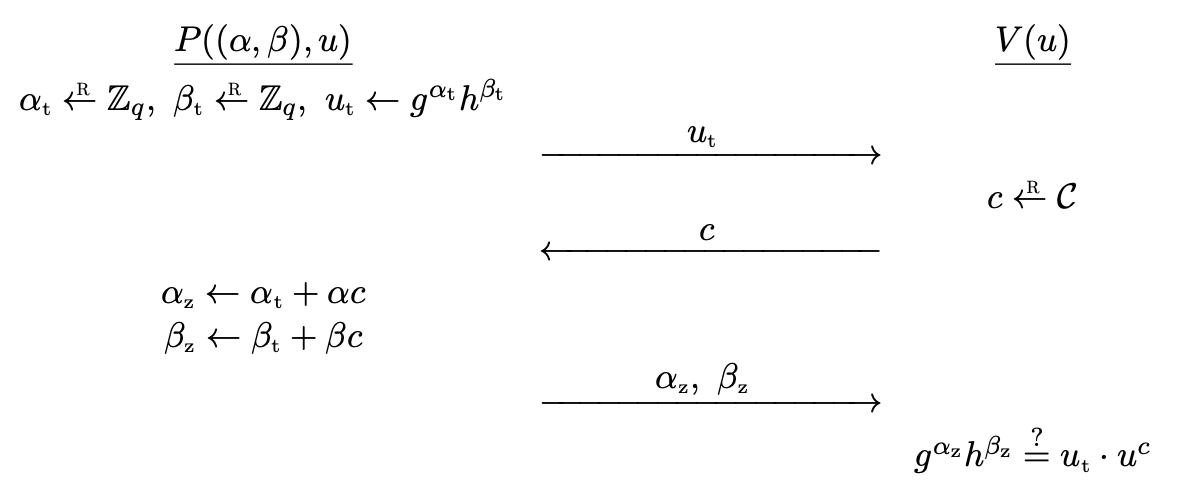
\includegraphics[width=0.75\linewidth]{figures/chapter19/fig6.png}
  \caption{Okamoto 协议}
  \label{fig:19-6}
\end{figure}

\begin{theorem}
Okamoto 协议是针对式 \ref{eq:19-11} 中定义的关系$\mathcal{R}$的一个 Sigma 协议。此外,Okamoto 协议提供知识健全性,且是特殊 HVZK 的。
\end{theorem}

\begin{proof}
显然,Okamoto 协议具有 Sigma 协议所要求的语法结构。陈述 $u\in\mathbb{G}$ 的一个接受对话形如:
$$
(u_{\rm t},c,(\alpha_{\rm z},\beta_{\rm z})) \text{~~s.t.~~} g^{\alpha_{\rm z}}h^{\beta_{\rm z}}=u_{\rm t}\cdot u^c
$$

\noindent
\emph{正确性.}
我们首先必须验证 Okamoto 协议是否满足基本的正确性要求,即诚实证明者和诚实验证者之间的交互总是能够产生一个接受对话。这很容易验证,因为如果:
$$
u_{\rm t}=g^{\alpha_{\rm t}}h^{\beta_{\rm t}},~~
\alpha_{\rm z}=\alpha_{\rm t}+\alpha c,~~
\beta_{\rm z}=\beta_{\rm t}+\beta c
$$
则我们有:
$$
g^{\alpha_{\rm z}}h^{\beta_{\rm z}}=
g^{\alpha_{\rm t}+\alpha c}h^{\beta_{\rm t}+\beta c}=
g^{\alpha_{\rm t}}h^{\beta_{\rm t}}\cdot(g^\alpha h^\beta)^c=
u_{\rm t}\cdot u^c
$$

\noindent
\emph{知识健全性.}
我们下面证明 Okamoto 协议提供知识健全性。假设我们现在有两个陈述 $u$ 的接受对话:
$$
(u_{\rm t},c,(\alpha_{\rm z},\beta_{\rm z})),~~
(u_{\rm t},c',(\alpha_{\rm z}',\beta_{\rm z}'))
$$
其中 $c\neq c'$。我们需要说明如何从这两个对话中有效提取 $u$ 的表示。这里的计算与 Schnorr 协议中的计算非常类似。注意到:
$$
g^{\alpha_{\rm z}}h^{\beta_{\rm z}}=u_{\rm t}\cdot u^c,~~
g^{\alpha_{\rm z}'}h^{\beta_{\rm z}'}=u_{\rm t}\cdot u^{c'}
$$
将第一个等式除以第二个等式,$u_{\rm t}$ 就被抵消了,于是我们有:
$$
g^{\Delta\alpha}h^{\Delta\beta}=u^{\Delta c},~~~~
\Delta\alpha:=\alpha_{\rm z}-\alpha_{\rm z}',~~
\Delta\beta:=\beta_{\rm z}-\beta_{\rm z}',~~
\Delta c:=c-c'
$$
因此,见证提取器可以用:
$$
\alpha\leftarrow{\Delta\alpha}/{c},~~
\beta\leftarrow{\Delta\beta}/{c}
$$
有效地计算出 $u$ 的一个表示 $(\alpha,\beta)\in\mathbb{Z}_q^2$。需要注意的是,由于 $c\neq c'$,$\Delta c$ 在 $\mathbb{Z}_q$ 中是可逆的。我们在这里利用了$q$是一个素数这个事实。

\vspace{5pt}

\noindent
\emph{特殊 HVZK.}
最后,我们通过给出一个模拟器来证明 Okamoto 协议是特殊 HVZK 的。这同样与 Schnorr 协议非常相似。对于输入 $u\in\mathbb{G}$ 和 $c\in\mathcal{C}$,模拟器计算:
$$
\alpha_{\rm z}\overset{\rm R}\leftarrow\mathbb{Z}_q,~~
\beta_{\rm z}\overset{\rm R}\leftarrow\mathbb{Z}_q,~~
u_{\rm t}\leftarrow{g^{\alpha_{\rm z}}h^{\beta_{\rm z}}}/{u^c}
$$
并输出 $(u_{\rm t},(\alpha_{\rm z},\beta_{\rm z}))$。可以发现,输出总是会产生一个符合要求的接受对话。

下面我们论证,当 $c\in\mathcal{C}$ 是随机选出的时候,模拟器在输入 $u,c$ 上的输出具有正确的分布。注意到在真实的对话中,$c$,$\alpha_{\rm z}$ 与 $\beta_{\rm z}$ 相互独立,其中 $c$ 在 $\mathcal{C}$ 上均匀分布,$\alpha_{\rm z}$ 和 $\beta_{\rm z}$ 在 $\mathbb{Z}_q$ 上均匀分布。此外,如果给定 $c$、$\alpha_{\rm z}$ 和 $\beta_{\rm z}$,$u_{\rm t}$ 的值由方程:

$$
g^{\alpha_{\rm z}}h^{\beta_{\rm z}}=u_{\rm t}\cdot u^c
$$
唯一决定。而这显然与模拟器的输出分布是一致的。
\end{proof}

\subsection{用于 DH 三元组的 Chaum-Pedersen 协议}\label{subsec:19-5-2}

Chaum-Pedersen 协议允许证明者在不向验证者透露任何其他信息的情况下,说服一个持怀疑态度的验证者相信一个给定的三元组是DH 三元组。

令 $\mathbb{G}$ 是一个 $q$ 阶循环群,其中 $q$ 是素数,$g\in\mathbb{G}$ 是生成元。回忆一下 10.5 节,对于 $\alpha,\beta,\gamma\in\mathbb{Z}_q$,如果 $\gamma=\alpha\beta$,我们就称元组 $(g^\alpha,g^\beta,g^\gamma)$ 为一个 DH 三元组 (DH-triple)。等价地,当且仅当存在 $\beta\in\mathbb{Z}_q$ 使得 $v=g^\beta$且$w=u^\beta$ 时,元组 $(u,v,w)$ 才是一个 DH 三元组。

Chaum-Pedersen 协议是关系:
\begin{equation}\label{eq:19-12}
\mathcal{R}:=\bigg\lbrace
\big(\beta, (u,v,w)\big)\in\mathbb{Z}_q\times\mathbb{G}^3:v=g^\beta, w=u^\beta
\bigg\rbrace
\end{equation}
上的 Sigma 协议。陈述 $(u,v,w)\in\mathbb{G}^3$ 的见证是使得 $v=g^\beta$ 且 $w=u^\beta$ 的一个 $\beta\in\mathbb{Z}_q$。因此,当且仅当陈述是一个 DH 三元组时,它才会存在一个见证。 与我们之前介绍的其它例子不同,在 Chaum-Pedersen 协议中,并非所有的陈述都必然存在见证。 

图 \ref{fig:19-7} 是 Chaum-Pedersen 协议 $(P,V)$ 的流程图,挑战空间 $\mathcal{C}$ 是 $\mathbb{Z}_q$ 的一个子集。

\begin{figure}
  \centering
  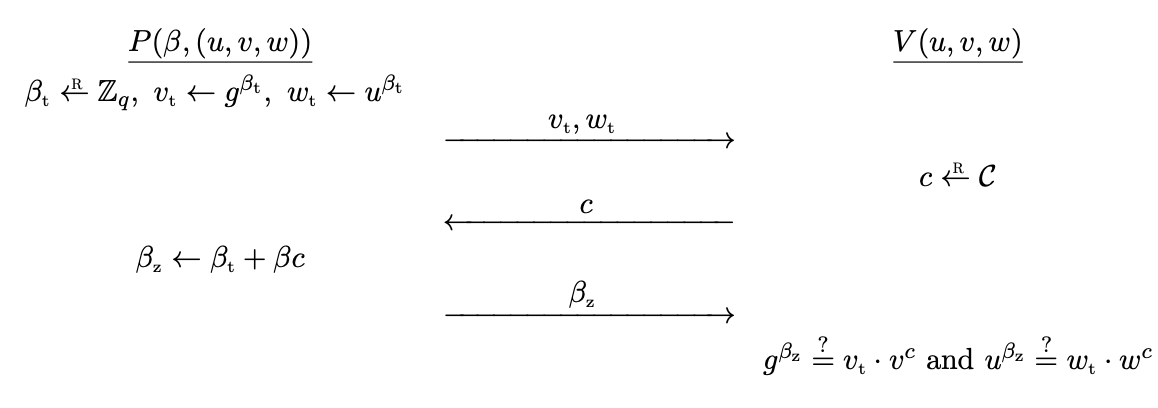
\includegraphics[width=0.75\linewidth]{figures/chapter19/fig7.png}
  \caption{Chaum-Pedersen 协议}
  \label{fig:19-7}
\end{figure}

\begin{theorem}
Chaum-Pedersen 协议是式 \ref{eq:19-12} 中定义的关系$\mathcal R$上的一个 Sigma 协议。此外,Chaum-Pedersen 协议提供知识健全性,且是特殊 HVZK 的。
\end{theorem}

\begin{proof}
显然,Chaum-Pedersen 协议具有 Sigma 协议所要求的语法结构。陈述 $(u,v,w)\in\mathbb{G}^3$ 的一个接受对话形如:
$$
((v_{\rm t},w_{\rm t}),c,\beta_{\rm z}) \text{~~s.t.~~} 
g^{\beta_{\rm z}}=v_{\rm t}\cdot v^c,~~
y^{\beta_{\rm z}}=w_{\rm t}\cdot w^c
$$
不难证明,一个诚实证明者与一个诚实验证者之间总是能够产生接受对话。

\noindent
\emph{知识健全性.}
假设我们有两个陈述 $(u,v,w)$ 的接受对话
$$
((v_{\rm t},w_{\rm t}),c,\beta_{\rm z}),~~
((v_{\rm t},w_{\rm t}),c',\beta_{\rm z}')
$$
其中 $c\neq c'$。不难发现
$$
\beta:={\Delta\beta}/{\Delta c}
$$
是陈述 $(u,v,w)\in\mathbb{G}^3$ 对应的见证,其中$\Delta\beta:=\beta_{\rm z}-\beta_{\rm z}'$,$\Delta c:=c-c'$。

\vspace{5pt}

\noindent
\emph{特殊 HVZK.}
对于输入 $(u,v,w)\in\mathbb{G}^3$ 和 $c\in\mathcal{C}$ 时,模拟器计算:
$$
\beta_{\rm z}\overset{\rm R}\leftarrow\mathbb{Z}_q,~~
v_{\rm t}\leftarrow{g^{\beta_{\rm z}}}/{v^c},~~
w_{\rm t}\leftarrow{u^{\beta_{\rm z}}}/{w^c}
$$
并输出 $((v_{\rm t},w_{\rm t}),c,\beta_{\rm z})$。可以发现,输出总是会产生一个符合要求的接受对话。

下面我们论证,当 $c\in\mathcal{C}$ 是随机选出的时候,模拟器在输入 $((u,v,w),c)$ 上的输出具有正确的分布。注意到在真实的对话中,$c$ 和 $\beta_{\rm z}$ 相互独立,其中 $c$ 在 $\mathcal{C}$ 上均匀分布,$\beta_{\rm z}$ 在 $\mathbb{Z}_q$ 上均匀分布。此外,如果给定 $c$ 和 $\beta_{\rm z}$,$v_{\rm t}$ 和 $w_{\rm t}$ 的值由
$$
g^{\beta_{\rm z}}=v_{\rm t}\cdot v^c, ~~
u^{\beta_{\rm z}} =w_{\rm t}\cdot w^c
$$
唯一决定。而这显然与模拟器的输出分布是一致的。
\end{proof}

\subsection{用于任意线性关系的 Sigma 协议}\label{subsec:19-5-3}

读者可能已经注意到 Schnorr、Okamoto 和 Chaum-Pedersen 协议之间的某些相似之处。事实上,它们都是用于证明一组元素之间线性关系的通用 Sigma 协议的特例。

与之前一样,令 $\mathbb{G}$ 是一个 $q$ 阶循环群,其中 $q$ 是素数,$g\in\mathbb{G}$ 是生成元。考察形如:
\begin{equation}\label{eq:19-13}
\phi(x_1,\dots,x_n):=
\left\{
~u_1=\prod^n_{j=1}g_{1j}^{x_j} ~~\land~~\cdots~~\land~~ u_m=\prod^n_{j=1}g_{mj}^{x_j}~
\right\}
\end{equation}
的布尔表达式 $\phi$。其中所有的 $g_{ij}$ 和 $u_i$ 都是 $\mathbb{G}$ 中的元素,这些元素中的有些可以是系统参数甚至是常数,有些是表达式特有的。$\phi$ 中的 $x_i$ 是公式的变量。当我们给 $x_1,\dots,x_n$ 赋 $\mathbb{Z}_q$ 中的值时,如果式 \ref{eq:19-13} 中的所有等式都成立,$\phi$ 就会输出 true。

对于这类公式的集合 $\mathcal{F}$,我们可以定义关系:
\begin{equation}\label{eq:19-14}
\mathcal{R}:=
\bigg\lbrace
\Big(
(\alpha_1,\dots,\alpha_n),\phi
\Big)
\in\mathbb{Z}_q^n\times\mathcal{F}: ~\phi(x_1,\dots,x_n)={\rm{true}}~
\bigg\rbrace
\end{equation}
因此,陈述是一个表达式 $\phi\in\mathcal{F}$,$\phi$ 的见证是能使得表达式 $\phi$ 输出 true 的 $x_1,\dots,x_n$ 的一组赋值 $(\alpha_1,\dots,\alpha_n)\in\mathbb{Z}_q^n$。我们之所以称其为``线性"关系集,是因为如果我们取离散对数,式 \ref{eq:19-13} 就可以改写为如下的线性方程组:
$$
{\rm\mathsf{Dlog}}_g(u_j)=\sum_{j=1}^nx_i\cdot {\rm\mathsf{Dlog}}_g(g_{ij})~~~~(i=1,2,\dots,m)
$$
而见证就是上述线性方程组的一组解。

\begin{figure}
  \centering
  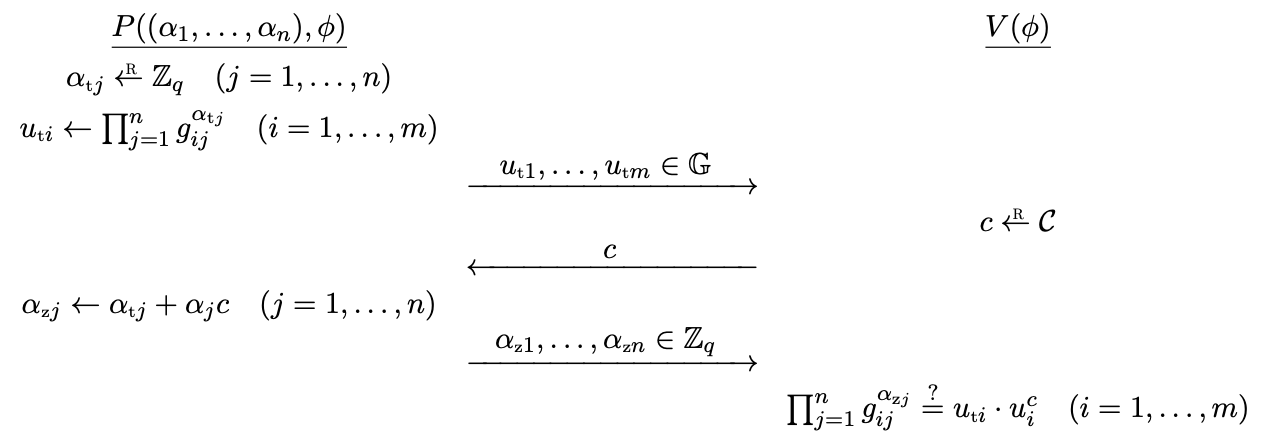
\includegraphics[width=0.85\linewidth]{figures/chapter19/fig8.png}
  \caption{通用线性协议}
  \label{fig:19-8}
\end{figure}

图 \ref{fig:19-8} 展示了关系 $\mathcal{R}$ 上的\textbf{通用线性协议 (generic linear protocol)} $(P,V)$。证明者拥有 $\phi$ 和见证 $(\alpha_1,\dots,\alpha_n)\in\mathbb{Z}_q^n$,挑战空间 $\mathcal{C}$ 是 $\mathbb{Z}_q$ 的一个子集。这样,到目前为止我们所介绍的所有 Sigma 协议都是这个通用线性协议的特例:
\begin{itemize}
	\item Schnorr 协议对应着 $\phi_1(x):=\{u=g^x\}$ 的情况。
	\item Okamoto 协议对应着 $\phi_2(x,y):=\{u=g^xh^y\}$ 的情况。
	\item Chaum-Pedersen 协议对应着 $\phi_3(x):=\{v=g^x\land w=u^x\}$ 的情况。
\end{itemize}

我们可以通过模仿Schnorr、Okamoto和Chaum-Pedersen的相应定理的证明来证明以下定理。我们把它作为一个练习留给读者。

\begin{theorem}\label{theo:19-11}
图 \ref{fig:19-8} 所描述的通用线性协议是式 \ref{eq:19-14} 中定义的关系 $\mathcal R$ 上的一个 Sigma 协议。此外,该协议提供知识健全性,且是特殊 HVZK 的。
\end{theorem}

我们还可以进一步泛化这个通用线性协议,方法是允许式 \ref{eq:19-13} 中的各个方程定义在不同的群上。唯一的要求是所有群都有相同的素阶 $q$。这种更通用的线性协议的典型出现场景是有两类方程,其中一类定义在密码学所感兴趣的群 $\mathbb{G}$ 上,群的阶为素数 $q$;另一类定义在 $\mathbb{Z}_q$ 上,其形式为 $\kappa_i=\sum_{j=1}^n\lambda_{ij}x_j$,其中 $\kappa_i$ 和 $\lambda_{ij}$ 是 $\mathbb{Z}_q$ 中的元素。

\subsection{一种用于同态原像的 Sigma 协议}

到目前为止我们介绍的所有 Sigma 协议,包括通用线性协议,都可以用群同态的语言来更清楚、更简洁地描述。令 $\mathbb{H}_1$ 和 $\mathbb{H}_2$ 是两个阶已知的有限阿贝尔群,$\psi:\mathbb{H}_1\to\mathbb{H}_2$ 是一个群同态。我们将群 $\mathbb{H}_1$ 中的运算表示为加法形式,将群 $\mathbb{H}_2$ 中的运算表示为乘法形式。

\begin{figure}
  \centering
  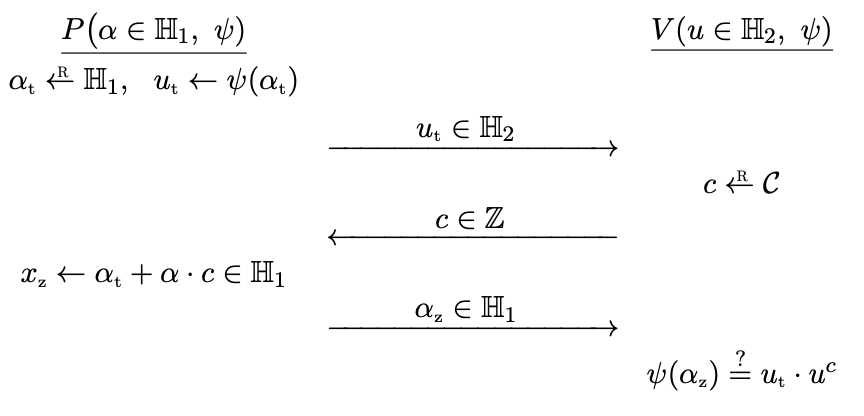
\includegraphics[width=0.6\linewidth]{figures/chapter19/fig9.png}
  \caption{用于同态原像的 Sigma 协议}
  \label{fig:19-9}
\end{figure}

令 $u\in\mathbb{H}_2$。图 \ref{fig:19-9} 展示了一个 Sigma 协议,它允许证明者说服验证者它``知道" $u$ 在 $\psi$ 下的原像。具体地,该协议是关系:
\begin{equation}\label{eq:19-15}
\mathcal{R}:=\bigg\lbrace
\Big(\alpha,(u,\psi)\Big)\in\mathbb{H}_1\times(\mathbb{H}_1\times\mathcal{F}):\psi(\alpha)=u
\bigg\rbrace
\end{equation}
上的一个 Sigma 协议。其中 $\alpha\in\mathbb{H}_1$ 是 $u\in\mathbb{H}_2$ 在 $\psi$ 下的原像。图 \ref{fig:19-9} 中的证明者持有见证 $\alpha\in\mathbb{H}_1$,验证者持有像 $u\in\mathbb{H}_2$,双方共有 $(\mathbb{H}_1,\mathbb{H}_2,\psi)$。挑战空间 $\mathcal{C}$ 为 $\{0,1,\dots,N-1\}\subseteq\mathbb{Z}$,其中 $N$ 为特定整数。

下面让我们看看这个协议是如何包含到目前为止所有的 Sigma 协议实例的。令 $\mathbb{G}$ 是一个素阶 $q$ 的群,且有生成元 $g,h,u\in\mathbb{G}$:
\begin{itemize}
	\item Okamoto 协议对应着 $\mathbb{H}_1:=\mathbb{Z}_q^2$,$\mathbb{H}_2:=\mathbb{G}$ 且 $\psi_1(x,y):=g^xh^y$ 的特殊情况。
	\item Chaum-Pedersen 协议对应着
	$$\mathbb{H}_1:=\mathbb{Z}_q,~~\mathbb{H}_2:=\mathbb{G}^2, ~~\psi_2(x):=(g^x,u^x)$$
	的特殊情况。我们甚至可以令 $\mathbb{H}_2=\mathbb{G}_1\times\mathbb{G}_2$,其中 $g\in\mathbb{G}_1$,$u\in\mathbb{G}_2$,并且 $|\mathbb{G}_1|=|\mathbb{G}_2|$。那么对于一个给定的 $(v,w)\in\mathbb{G}_1\times\mathbb{G}_2$,提供$(v, w)$ 在 $\psi_2$ 上的一个原像与计算群 $\mathbb{G}_1$ 和 $\mathbb{G}_2$ 上的离散对数问题 $\mathsf{Dlog}_g(v)=\mathsf{Dlog}_u(w)$ 等价。
	\item 图 \ref{fig:19-8} 中的通用线性协议对应着
	$$
    \mathbb{H}_1:=(\mathbb{Z}_q)^n,~~
    \mathbb{H}_2:=\mathbb{G}^m,~~
    \psi_3(x_1,\dots,x_n):=
    \left(
    ~\prod_{j=1}^ng_{1j}^{x_j},~\dots,~\prod_{j=1}^ng_{mj}^{x_j}~
    \right)
    $$
    的特殊情况。其中,对于所有的$i=1,\dots,m$和$j=1,\dots,n$,都有$g_{ij}\in\mathbb{G}$。
\end{itemize}
我们可以很容易地验证 $\psi_1,\psi_2,\psi_3$ 的映射都是群同态的。通过在图 \ref{fig:19-9} 中的协议使用这些同态映射,我们可以得到本节中介绍的所有 Sigma 协议实例。

\begin{theorem}\label{theo:19-12}
图 \ref{fig:19-9} 中的协议是式 \ref{eq:19-15} 中定义的关系 $\mathcal R$ 上的一个 Sigma 协议。此外,该协议是特殊 HVZK 的,而且只要 $|\mathbb{H}_1|\times|\mathbb{H}_2|$ 的最小素因子至少是 $|\mathcal{C}|$,该协议就提供知识健全性。
\end{theorem}

定理 \ref{theo:19-12} 的证明完全模仿了 Schnorr 协议相应定理的证明。对 $|\mathbb{H}_1|\times|\mathbb{H}_2|$ 的最小素因子的下限要求,是为了确保见证提取器可以从两个接受对话 $(u_{\rm t},c,\alpha_{\rm z})$ 和 $(u_{\rm t},c',\alpha_{\rm z}')$ 中获得一个映射 $\psi$ 的原像。就如同在 Schnorr 协议中的见证提取器中那样,我们可以得到$\psi(\Delta\alpha)=u^{\Delta c}$,其中$\Delta\alpha:=(\alpha_z-\alpha_z')\in\mathbb{H}_1$,$\Delta c=(c-c')\in\mathbb{Z}$。限制 $|\mathbb{H}_1|$ 和 $|\mathbb{H}_2|$ 素因子的下界是为了确保(1)我们可以在 $\mathbb{H}_1$ 中用 $\Delta c$ 除以 $\Delta\alpha$,并且(2)我们可以在等式两边同时升幂 $((\Delta c)^{-1}\mod |\mathbb{H}_2|)\in\mathbb{Z}$,以求得等式右项的 $\Delta c$ 次方根。然后,我们就可以得到$\psi({\Delta\alpha}/{\Delta c})=u$,因此 ${\Delta\alpha}/{\Delta c}\in\mathbb{H}_1$ 就是 $u\in\mathbb{H}_2$ 在映射 $\psi$ 下的原像。

\subsection{一种用于 RSA 的 Sigma 协议}\label{subsec:19-5-5}

为了避免读者认为 Sigma 协议只适用于与离散对数有关的问题,我们下面介绍一个与 RSA 有关的协议。

令 $(n,e)$ 是一个 RSA 公钥,$e$ 是一个素数。我们将 $(n,e)$ 视为一个系统参数。Guillou-Quisquater (GQ) 协议允许证明者说服持怀疑态度的验证者,它``知道" $y\in\mathbb{Z}_n^*$ 的一个 $e$ 次方根,而不透露任何其他信息。更确切地说,GQ 协议是关系:
\begin{equation}\label{eq:19-16}
\mathcal{R}=
\bigg\lbrace
(x,y)\in\mathbb{Z}_n^*\times\mathbb{Z}_n^*:x^e=y
\bigg\rbrace
\end{equation}
上的一个 Sigma 协议。陈述 $y\in\mathbb{Z}_n^*$ 的见证是 $x\in\mathbb{Z}_n^*$,满足 $x^e=y$。由于 $(n,e)$ 是一个 RSA 公钥,因此由 $x\in\mathbb{Z}_n^*$ 到 $y=x^e\in\mathbb{Z}_n^*$ 的映射是一个双射。因此每个陈述都对应着唯一的见证。

\begin{figure}
  \centering
  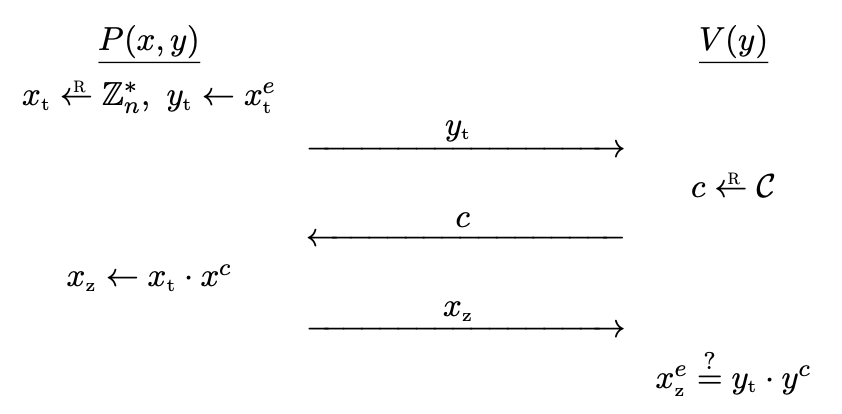
\includegraphics[width=0.6\linewidth]{figures/chapter19/fig10.png}
  \caption{Guillou-Quisquater 协议}
  \label{fig:19-10}
\end{figure}


图 \ref{fig:19-10} 展示了 GQ 协议 $(P,V)$ 的工作流程。其挑战空间 $\mathcal{C}$ 是 $\{0,\dots,e-1\}$ 的一个子集。需要注意的是,当 $e$ 很小时,挑战空间也很小。如果需要,我们可以用练习 19.5 中介绍的方法将其扩大。然而在使用该协议时,我们通常会将 $e$ 设定为一个大素数来确保挑战空间是足够大的。

图 \ref{fig:19-10} 中的 GQ 协议也是图 \ref{fig:19-9} 中展示的用于同态原像的 Sigma 协议的一个特例。此时群同态是 $\psi:\mathbb{Z}_n^*\to\mathbb{Z}_n^*$,定义为 $\psi(x)=x^e$。然而,我们无法像定理 \ref{theo:19-12} 那样证明 GO 协议提供知识健全性,因为群 $\mathbb{Z}_n^*$ 的阶是未知的。相反地,我们必须对这些属性进行单独证明。我们有下面的定理。

\begin{theorem}
GQ协议是式 \ref{eq:19-16} 中定义的关系$\mathcal R$上的一个Sigma协议。此外,它提供知识健全性,并且是特殊HVZK的。
\end{theorem}

\begin{proof}
$y$ 的一个接受对话形如 $(x_{\rm t},c,x_{\rm z})$,其中 $x^e_{\rm z}=y_{\rm t}\cdot y^c$。读者很容易验证基本的正确性要求,即一个诚实证明者和一个诚实验证者之间的交互总是会产生一个接受对话。

\vspace{5pt}

\noindent
\emph{知识健全性.}
下面我们将证明 GQ 协议具备知识健全性。假设我们有两个陈述 $y$ 的接受对话 $(x_{\rm t},c,x_{\rm z})$ 和 $(x_{\rm t},c',x_{\rm z}')$,其中 $c\neq c'$。我们必须证明能够有效计算出 $y$ 的 $e$ 次方根。观察到:
$$
x^e_{\rm z}=y_{\rm t}\cdot y^c,~~
(x_{\rm z}')^e=y_{\rm t}\cdot y^{c'}
$$
将第一个方程除以第二个方程,可以得到:
$$
(\Delta x)^e=y^{\Delta c}
$$
其中:$\Delta x:={x_{\rm z}}/{x_{\rm z}'}$,$\Delta c:=c-c'$。由于 $c\neq c'$,且 $c$ 和 $c'$ 都属于区间 $\{0,\dots,e-1\}$,因此有 $0<|\Delta c|<e$,所以 $e\nmid\Delta c$。此外由于 $e$ 是素数,所以 $\gcd(e,\Delta c)=1$。因此当给定 $e$,$f:=\Delta c$,$w:=\Delta x$ 时,我们可以利用定理 10.6 求得 $y$ 的 $e$ 次方根。

读者应该注意到,这里给出的从两个接受对话中计算 RSA 逆变换的技术与定理 10.7 的证明中使用的方法基本相同。事实上,这两个接受对话制造了哈希函数 $H_{\rm rsa}(a,b)=a^ey^b$ 上的一次碰撞 $((x_{\rm z},-c\mod e),(x_{\rm z}',-c'\mod e))$。

\vspace{5pt}

\noindent
\emph{特殊 HVZK.}
最后,我们通过给出一个模拟器来证明 GQ 协议是特殊 HVZK 的。对于输入 $y\in\mathbb{Z}_n^*$ 和 $c\in\mathcal{C}$,模拟器计算:
$$
x_{\rm z}\overset{\rm R}\leftarrow\mathbb{Z}_n^*,~~
y_{\rm t}\leftarrow{x_{\rm z}^e}/{y^c}
$$
并输出 $(y_{\rm t},x_{\rm z})$。注意到在真实的对话中,$c$ 和 $x_{\rm z}$ 是相互独立的,$c$ 在 $\mathcal{C}$ 上均匀分布,$x_z$ 在 $\mathbb{Z}_n^*$ 上均匀分布。此外,如果给定 $c$ 和 $x_z$,$y_t$ 的值由方程$x^e_{\rm z}=y_{\rm t}\cdot y^c$唯一决定。而这显然与模拟器的输出分布是一致的。
\end{proof}
\section{基于Sigma协议的身份识别和签名}\label{sec:19-6}

通过模仿 Schnorr 构造,我们很容易将任何 Sigma 协议转换成相应的识别方案和签名方案。

假设我们有一个关系 $\mathcal{R}\subseteq\mathcal{X}×\mathcal{Y}$ 上的 Sigma 协议 $(P,V)$。除了算法 $P$ 和 $V$ 之外,我们还需要一个 $\mathcal{R}$ \textbf{上的密钥生成算法}。它是一个概率算法 $G$,生成一个公私钥对 $(pk,sk)$,其中 $pk=y$,$sk=(x,y)$,$(x,y)\in\mathcal{R}$。

为了得到安全的识别和签名方案,我们需要以下的``单向性"特征:给定 $G$ 输出的公钥 $pk=y\in\mathcal{Y}$,应该很难计算出一个 $\hat x\in\mathcal{X}$ 满足 $(\hat x,y)\in\mathcal{R}$。我们用下面的攻击游戏来更加精准地描述这个概念。

\begin{game}[单向密钥生成]\label{game:19-2}
令 $G$ 是 $\mathcal{R}\subseteq\mathcal{X}×\mathcal{Y}$ 上的一个密钥生成算法。对于一个给定对手 $\mathcal{A}$,攻击游戏按如下方式运行:
\begin{itemize}
	\item 挑战者运行 $(pk,sk)\overset{\rm R}\leftarrow G()$,并将 $pk=y$ 发送给 $\mathcal{A}$;
	\item $\mathcal{A}$ 输出 $\hat x\in\mathcal{X}$。
\end{itemize}
如果 $(\hat x,y)\in\mathcal{R}$,我们就称对手赢得了攻击游戏。我们将 $\mathcal{A}$ 相对于 $\mathbb{G}$ 的优势定义为 ${\rm OW\mathsf{adv}}[\mathcal{A},\mathbb{G}]$,其值为 $\mathcal{A}$ 赢得游戏的概率。
\end{game}

\begin{definition}
如果对于所有有效对手 $\mathcal{A}$,${\rm OW\mathsf{adv}}[\mathcal{A},\mathbb{G}]$ 的值都是可忽略不计的,我们就称密钥生成算法 $G$ 是\textbf{单向的}。
\end{definition}

\begin{example}\label{exmp:19-4}
对于例 \ref{exmp:19-1} 介绍的 Schnorr的Sigma 协议,最自然的密钥生成算法是计算 $\alpha\overset{\rm R}\leftarrow\mathbb{Z}_q$ 和 $u\leftarrow g^\alpha\in\mathbb{G}$,并输出 $pk:=u$ 和 $sk:=(\alpha,u)$。在离散对数假设下,这种密钥生成算法显然是单向的。
\end{example}

\begin{example}\label{exmp:19-5}
考虑 \ref{subsec:19-5-5} 小节介绍的 GQ 协议,其中 RSA 公钥 $(n, e)$ 被视为一个系统参数。最自然的密钥生成算法是计算 $x\overset{\rm R}\leftarrow\mathbb{Z}_n^*$ 和 $y\leftarrow x^e\in\mathbb{Z}_n^*$,并输出 $pk:=y$ 和 $sk:=(x,y)$。在 RSA 假设下,这种密钥生成算法显然也是单向的(见定理10.5)。
\end{example}

一个含有密钥生成算法 $G$ 的 Sigma 协议 $(P,V)$ 能够提供一个身份识别方案 $(G,P,V)$。接下来的两个定理将证明它对窃听攻击是安全的。

\begin{theorem}
令 $(P,V)$ 是一个具有大挑战空间的有效关系 $\mathcal{R}$ 上的 Sigma 协议。令 $G$ 是$\mathcal{R}$ 的一个密钥生成算法。如果 $(P,V)$ 提供知识健全性,并且 $G$ 是单向的,那么身份识别方案 $\mathcal{I}:=(G,P,V)$ 对于直接攻击是安全的。

\begin{quote}
特别地,假设 $\mathcal{A}$ 是一个有效冒充对手,他通过攻击游戏 \ref{game:18-1} 中的直接攻击来攻击 $\mathcal{I}$,其优势为 $\epsilon:=\rm{ID1\mathsf{adv}}[\mathcal{A},\mathcal{I}]$。则必然存在一个有效对手 $\mathcal{B}$如攻击游戏 \ref{game:19-2} 那样攻击 $G$,其运行时间大约是 $\mathcal{A}$ 的两倍,其优势 $\epsilon':={\rm OW\mathsf{adv}}[\mathcal{A},\mathbb{G}]$,那么:
\end{quote}
\begin{equation}\label{eq:19-17}
\epsilon'\geq \epsilon^2-\frac{\epsilon}{N}
\end{equation}
\begin{quote}
其中 $N$ 是挑战空间的大小,这意味着:
\end{quote}
\begin{equation}\label{eq:19-18}
\epsilon\leq\frac{1}{N}+\sqrt{\epsilon'}
\end{equation}
\end{theorem}

\begin{proof}
我们可以模仿定理 \ref{theo:19-1} 的证明。利用冒充对手 $\mathcal{A}$,我们可以使用下述方法建立一个打破 $G$ 的单向性的对手 $\mathcal{B}$。对手 $\mathcal{B}$ 从其挑战者那里得到一个公钥 $pk = y$,而我们的目标是让 $\mathcal{B}$ 在 $\mathcal{A}$ 的帮助下计算出一个满足 $(\hat x,y)\in\mathcal{R}$的$\hat x$。$\mathcal{B}$ 的行为可以分为两个阶段。

在第一阶段,$\mathcal{B}$ 扮演 $\mathcal{A}$ 的挑战者的角色,给 $\mathcal{A}$ 提供值 $pk=y$ 作为验证公钥。使用与定理 \ref{theo:19-1} 的证明中相同的回溯方法,对手 $\mathcal{B}$ 可以以至少 $\epsilon^2-{\epsilon}/{N}$ 的概率获得 $y$ 的两个接受对话 $(t,c,z)$ 和 $(t,c',z')$,其中 $c\neq c'$。更具体地说,$\mathcal{B}$ 等待来自 $\mathcal{A}$ 的承诺 $t$,接着向 $\mathcal{A}$ 发送一个随机挑战 $c$,并等待 $\mathcal{A}$ 的应答 $z$。在此之后,$\mathcal{B}$ 将 $\mathcal{A}$ 的内部状态回溯到它产生 $t$ 的那一时刻,然后向 $\mathcal{A}$ 发送另一个随机挑战 $c'$,并等待 $\mathcal{A}$ 的应答 $z'$。根据回溯引理(引理\ref{theo:19-2}),这个过程将以至少 $\epsilon^2-{\epsilon}/{N}$ 的概率产生两个接受对话。

在计算的第二阶段,$\mathcal{B}$ 将这两个接受对话送入见证提取器(由知识健全性保证存在),以为 $y$ 提取一个见证 $\hat x$。

这样我们就证明了式 \ref{eq:19-17},而式 \ref{eq:19-18}可以通过与定理 \ref{theo:19-1} 相同的方式得到。
\end{proof}

定理 \ref{theo:19-3} 显然适用于从特殊 HVZK 的 Sigma 协议衍生出来的身份识别协议:

\begin{theorem}\label{theo:19-15}
令 $(P,V)$ 是一个有效关系 $\mathcal{R}$ 上的 Sigma 协议。令 $G$ $\mathcal{R}$ 的一个密钥生成算法。如果一个身份识别协议 $\mathcal{I}=(G,P,V)$ 对于直接攻击是安全的,且$(P,V)$是特殊 HVZK 的,那么 $\mathcal{I}$ 对于窃听攻击也是安全的。
\begin{quote}
特别地,对于每一个通过攻击游戏 18.2 中的窃听攻击来攻击 $\mathcal{I}$ 的冒充对手 $\mathcal{A}$,必然存在一个通过攻击游戏 \ref{game:18-1} 中的直接攻击来攻击 $\mathcal{I}$ 的对手 $\mathcal{B}$,其中 $\mathcal{B}$ 是 $\mathcal{A}$ 的一个基本包装器,使得:
\end{quote}
$$
{\rm ID2\mathsf{adv}}[\mathcal{A},\mathcal{I}]=
{\rm ID1\mathsf{adv}}[\mathcal{B},\mathcal{I}]
$$
\end{theorem}

\begin{example}\label{exmp:19-6}
如果我们用例 \ref{exmp:19-5} 中的密钥生成算法 $G$ 来增强 GQ 协议 $(P,V)$,我们就能够得到识别方案 $\mathcal{I}_{\rm GQ}=(G,P,V)$,只要挑战空间足够大,该识别方案在 RSA 假设下对窃听攻击就是安全的。
\end{example}

\subsection{用于签名的 Fiat-Shamir 启发式算法}\label{subsec:19-6-1}

使用 \ref{sec:19-2} 节中介绍的技术,我们就可以将 Sigma 协议转换为签名方案。这个普适的技术最早由 Fiat 和 Shamir 提出,它包含如下几个部分:
\begin{itemize}
	\item 一个关系 $\mathcal{R}\subseteq\mathcal{X}×\mathcal{Y}$ 上的 Sigma 协议 $(P,V)$。我们假设对话形如 $(t,c,z)$,其中 $t\in\mathcal{T}$,$c\in\mathcal{C}$,$z\in\mathcal{Z}$;
	\item 一个关系 $\mathcal{R}$ 的密钥生成算法 $G$;
	\item 一个哈希函数 $H:\mathcal{M}\times\mathcal{T}\to\mathcal{C}$,它被建模为一个随机预言机。集合 $\mathcal{M}$ 也同样是签名方案的消息空间。
\end{itemize}

由 $G$ 和 $(P, V)$ 派生出的\textbf{Fiat-Shamir 签名方案}的工作原理如下:
\begin{itemize}
	\item 密钥生成算法为 $G$,所以公钥形如 $pk=y$, 其中$y\in\mathcal{Y}$,私钥形如 $sk=(x,y)\in\mathcal{R}$。
	\item 使用私钥 $sk = (x, y)$ 对消息 $m\in\mathcal{M}$ 进行签名,签名算法运行如下:
	\begin{itemize}
		\item 运行验证者 $P(x,y)$ 并获得一个承诺 $t\in\mathcal{T}$;
		\item 计算挑战 $c\leftarrow H(m,t)$;
		\item 最后,将 $c$ 发送给证明者并得到一个应答 $z$,然后输出签名 $\sigma:=(t,z)\in\mathcal{T}\times\mathcal{Z}$。
	\end{itemize}
	\item 为了使用公钥 $pk=y$ 验证对消息 $m\in\mathcal{M}$ 的签名 $\sigma=(t,z)\in\mathcal{T}\times\mathcal{Z}$,验证算法计算 $c\leftarrow H(m,t)$,并检查 $(t,c,z)$ 是否是 $y$ 的接受对话。
\end{itemize}

正如我们对 Schnorr 协议所做的那样,我们下面会证明如果对应的识别方案 $(G,P,V)$ 对窃听攻击是安全的,那么 Fiat-Shamir 签名方案在随机预言机模型下是安全的。然而,我们还需要一个技术上的假设,基本上所有我们感兴趣的 Sigma 协议都满足这个假设。

\begin{definition}[不可预测承诺]\label{def:19-7}
令 $(P,V)$ 是关系 $\mathcal{R}\subseteq\mathcal{X}×\mathcal{Y}$ 上的 Sigma 协议,并假定所有对话 $(t,c,z)$ 都位于 $\mathcal{T}\times\mathcal{C}\times\mathcal{Z}$ 中。如果对于任意 $(x,y)$ 和 $\hat t\in\mathcal{T}$,$P(x,y)$ 和 $V(y)$ 之间的交互会以最多 $\delta$ 的概率产生一个对话 $(t,c,z)$ 满足 $t=\hat t$,则称 $(P,V)$ 有 \textbf{$\delta$-不可预测承诺 ($\delta$-unpredictable commitments)}。如果 $(P,V)$ 有 $\delta$-不可预测承诺,且 $\delta$ 的值不可忽略不计,我们就称 $(P,V)$ 有不可预测承诺。
\end{definition}

\begin{theorem}\label{theo:19-16}
如果 $H$ 被建模为一个随机预言机,身份识别方案 $\mathcal{I}=(G,P,V)$ 对窃听攻击是安全的,并且 $(P,V)$ 有不可预测承诺,那么从 $G$ 和 $(P, V)$ 派生出的 Fiat-Shamir 签名方案 $\mathcal{S}$ 是安全的。
\begin{quote}
	特别地,令 $\mathcal{A}$ 是一个像在攻击游戏 13.1 的随机预言机版本中一样的攻击 $\mathcal{S}$ 的对手。此外,假设 $\mathcal{A}$ 最多可以发起 $Q_{\rm s}$ 次签名查询和 $Q_{\rm ro}$ 次随机预言机查询,并且 $(P, V)$ 有 $\delta$-不可预测承诺。那么必然存在一个 $(Q_{\rm ro}+1)$ 次重复冒充攻击对手 $\mathcal{B}$,它能够通过攻击游戏 \ref{game:19-1} 中的窃听攻击来攻击 $\mathcal{I}$,其中 $\mathcal{B}$ 是 $\mathcal{A}$ 的一个基本包装器,使得:
\end{quote}
$$
{\rm SIG^{ro}\mathsf{adv}}[\mathcal{A},\mathcal{S}]\leq Q_{\rm s}(Q_{\rm s}+Q_{\rm ro}+1)\delta+{\rm rID2\mathsf{adv}}[\mathcal{B},\mathcal{I},Q_{\rm ro}+1]
$$
\end{theorem}

这个定理的证明与定理 \ref{theo:19-7} 的证明几乎相同,读者可以尝试自己证明该定理。

把以上结论结合起来,假设我们从一个 Sigma 协议 $(P, V)$ 开始,该协议是特殊 HVZK 的,并且它能提供知识健全性。此外,假设 $(P, V)$ 有不可预测承诺和一个大的挑战空间。那么,如果我们把 $(P, V)$ 和一个单向密钥生成算法 $G$ 结合起来,就可以利用 Fiat-Shamir 签名构造法基于一个随机预言机 $H$ 构建一个安全的签名方案。事实上,Schnorr 签名方案就是这个结构的一个特例。

就像我们对 Schnorr 签名所做的那样,我们也可以使用引理 \ref{theo:19-6} 将问题从 $r$ 次重复冒充规约到 $1$ 次冒充。但是更严格的规约也是有可能的,事实上引理 \ref{theo:19-8} 的证明在这里也是成立的,基本上不需要更改太多内容:

\begin{lemma}\label{theo:19-17}
令 $(P,V)$ 是一个关系 $\mathcal{R}\subseteq\mathcal{X}×\mathcal{Y}$ 上的特殊 HVZK 的 Sigma 协议,$G$ 是 $\mathcal{R}$ 上的一个密钥生成算法,考虑由此产生的身份识别协议 $\mathcal{I}=(G,P,V)$。假设 $\mathcal{A}$ 是一个如攻击游戏 \ref{game:19-1} 中那样的针对 $\mathcal{I}$ 的有效的 $r$ 次重复冒充窃听攻击对手,其优势为 $\epsilon:={\rm rID2\mathsf{adv}}[\mathcal{A},\mathcal{I},r]$。那么必然存在一个如攻击游戏 19.2 中那样的针对 $G$ 的有效对手 $\mathcal{B}$,其运行时间大约是 $\mathcal{A}$ 的两倍,其优势为 $\epsilon:={\rm OW\mathsf{adv}}[\mathcal{B},G]$,使得:
\begin{equation}
\epsilon'\geq\frac{\epsilon^2}{r}-\frac{\epsilon}{N}
\end{equation}
其中 $N$ 是挑战空间的大小,这意味着:
\begin{equation}\label{eq:19-20}
\epsilon\leq\frac{r}{N}+\sqrt{r\epsilon'}
\end{equation}
\end{lemma}

利用这一点,在 $(P, V )$ 是特殊 HVZK 的情况下,我们可以进一步确定定理 \ref{theo:19-16} 中给出的安全上界:

\begin{quote}
\emph{假设 $\mathcal{A}$ 是一个如攻击游戏 13.1 的随机预言机版本那样攻击 $\mathcal{S}$ 的有效对手。此外,假设 $\mathcal{A}$ 最多发起 $Q_{\rm s}$ 次签名查询和 $Q_{\rm ro}$ 次随机预言机查询。那么必然存在一个如攻击游戏 \ref{game:19-2} 中那样的针对 $G$ 的有效对手 $\mathcal{B}$,其运行时间大约是 $\mathcal{A}$ 的两倍,使得:}
\end{quote}
\begin{equation}
{\rm SIG^{ro}\mathsf{adv}}[\mathcal{A},\mathcal{S}]\leq Q_{\rm s}(Q_{\rm s}+Q_{\rm ro}+1)\delta+\frac{Q_{\rm ro}+1}{N}+\sqrt{(Q_{\rm ro}+1)\cdot{\rm OW\mathsf{adv}}[\mathcal{B},G]}
\end{equation}
\begin{quote}
\emph{其中 $N$ 是挑战空间的大小。}
\end{quote}

\subsubsection{GQ 签名方案}

将上面介绍的 Fiat-Shamir 签名构造应用于 GQ 协议(见 \ref{subsec:19-5-5} 小节),我们就可以构造出一个基于 RSA 的新签名方案。该方案利用 RSA 公钥 $(n,e)$ 作为系统参数,其中的指数 $e$ 是一个大素数。如果有需要的话,该系统参数可以被许多用户共享。我们需要一个哈希函数 $H:\mathcal{M}\times\mathcal{T}\to\mathcal{C}$,其中 $\mathcal{T}$ 是由 $\mathbb{Z}_n^*$ 中的所有元素编码后组成的集合,$\mathcal{M}$ 是签名方案的消息空间,$\mathcal{C}$ 是 $\{0,\dots,e-1\}$ 的一个子集。GQ 签名方案 $\mathcal{S}_{\rm GQ}=(G,S,V)$ 的组成部分如下:
\begin{itemize}
	\item 密钥生成算法 $G$ 计算:
	$$
    x\overset{\rm R}\leftarrow\mathbb{Z}_n^*,~~
    y\leftarrow x^e
    $$
	公钥为 $pk:=y$,私钥为 $sk:=x$。
	\item 为了使用私钥 $sk=x$ 对消息 $m\in\mathcal{M}$ 签名,签名算法$S(sk,m)$计算:
    $$
    x_{\rm t}\overset{\rm R}\leftarrow \mathbb{Z}_n^*,~~
    y_{\rm t}\leftarrow x_{\rm t}^e,~~
    c\leftarrow H(m,y_{\rm t}),~~
    x_{\rm z}\leftarrow x_{\rm t}\cdot x^c
    $$
    输出签名 $\sigma:=(y_{\rm t},x_{\rm z})$。
	\item 为了使用公钥 $pk=y$ 验证对消息 $m\in\mathcal{M}$ 的签名  $\sigma=(y_{\rm t},x_{\rm z})$,签名验证算法 $V$ 计算 $c:=H(m,y_t)$,当$x_{\rm z}^e=y_{\rm t}\cdot y^c$时输出$\mathsf{accept}$,否则输出$\mathsf{reject}$。
\end{itemize}    

正如我们在例 \ref{exmp:19-6} 中看到的那样,在 RSA 假设下,只要挑战空间足够大,GQ 识别方案对窃听攻击就是安全的。另外,可以观察到 GQ 协议有 ${1}/{\phi(n)}$-不可预测承诺。由定理 \ref{theo:19-16} 可知,在 RSA 假设下,相应的签名方案在随机预言机模型下是安全的。

GQ 签名相比 RSA 签名(如 $\mathcal{S}_{\rm RSA-FDH}$)的优势在于,它的签名算法要快得多。使用 $\mathcal{S}_{\rm RSA-FDH}$ 签名需要进行一个大指数运算,而 GQ 签名虽然需要进行 $e$ 和 $c$ 这两个指数运算,但这两个指数都只有 $128$ 位。当签名者是一个计算力孱弱的设备时,快速签名的能力是很重要的,比如使用芯片的信用卡在每笔交易中签名的场景。

\begin{snote}[一个优化.]
GQ 签名方案可以用和 Schnorr 签名方案相同的方式进行优化。在之前,我们定义的对消息 $m$ 的签名是一个数对  $(y_{\rm t},x_{\rm z})$,它满足:
$$
x_{\rm z}^e=y_{\rm t}\cdot y^c
$$
其中 $c:=H(m,y_{\rm t})$。为了进一步优化该签名方案,我们可以将签名定义为数对 $(c,x_{\rm z})$,它满足:
$$
c=H(m,y_{\rm t})
$$
其中 $y_{\rm t}:={x_{\rm z}^e}/{y^c}$。此外,我们可以在公钥中存储 $y^{-1}$ 而不是 $y$,这能够进一步将加快验证速度。

事实证明,这种优化也可以应用于Fiat-Shamir签名构造的大多数实例,参见练习 19.17。
\end{snote}

\section{Sigma协议的组合:AND和OR证明}

在本节中,我们将展示如何将 Sigma 协议组合起来构成新的 Sigma 协议。在 AND 证明结构中,证明者可以说服验证者它``知道"一对陈述的见证。在 OR 证明结构中,证明者可以说服验证者它``知道"两个陈述中其中一个的见证。

\subsection{AND 证明构造}

假设我们有一个 $\mathcal{R}_0\subseteq\mathcal{X}_0\times\mathcal{Y}_0$ 上的 Sigma 协议 $(P_0,V_0)$ 和一个 $\mathcal{R}_1\subseteq\mathcal{X}_1\times\mathcal{Y}_1$ 上的 Sigma 协议 $(P_1,V_1)$。此外,我们假设这两个 Sigma 协议都使用相同的挑战空间 $\mathcal{C}$。我们可以把它们组合起来构造一个关系:
\begin{equation}\label{eq:19-22}
\mathcal{R}_{\rm AND}=
\bigg\lbrace
\big((x_0,x_1),(y_0,y_1)\big)\in\left(\mathcal{X}_0\times\mathcal{X}_1\right)\times\left(\mathcal{Y}_0\times\mathcal{Y}_1\right):~(x_0,y_0)\in\mathcal{R}_0,~(x_1,y_1)\in\mathcal{R}_1
\bigg\rbrace
\end{equation}
上的 Sigma 协议。换句话说,给定一对陈述 $y_0\in\mathcal{Y}_0$ 和 $y_1\in\mathcal{Y}_1$,这个 \textbf{AND 协议}允许证明者说服持怀疑态度的验证者,它同时``知道" $y_0$ 的一个见证\emph{和} $y_1$ 的一个见证。该协议 $(P,V)$ 运行如下,其中验证者 $P$ 由 $((x_0,x_1),(y_0,y_1))\in\mathcal{R}_{\rm AND}$ 初始化,验证者 $V$ 由 $(y_0,y_1)\in\mathcal{Y}_0\times\mathcal{Y}_1$ 初始化:
\begin{enumerate}
	\item $P$ 运行 $P_0(x_0,y_0)$ 得到一个承诺 $t_0$,运行 $P_1(x_1,y_1)$ 得到一个承诺 $t_1$,并将承诺对 $(t_0,t_1)$发送给 $V$;
	\item $V$ 选取 $c\overset{\rm R}\leftarrow\mathcal{C}$,并将挑战 $c$ 发送给 $P$;
	\item $P$ 将挑战 $c$ 投入 $P_0(x_0,y_0)$ 和 $P_1(x_1,y_1)$,得到应答 $z_0$ 和 $z_1$,并将应答对 $(z_0,z_1)$ 发送给 $V$;
	\item $V$ 检查 $(t_0,c,z_0)$ 是否是 $y_0$ 的一个接受对话,$(t_1,c,z_1)$ 是否是 $y_1$ 的一个接受对话。
\end{enumerate}

\begin{theorem}
AND 协议 $(P,V)$ 是式 \ref{eq:19-22} 中定义的关系$\mathcal{R}_{\rm AND}$上的 Sigma 协议。若 $(P_0,V_0)$ 和 $(P_1,V_1)$ 提供知识健全性,则 $(P, V)$ 亦然。若 $(P_0,V_0)$ 和 $(P_1,V_1)$ 都是特殊 HVZK 的,则 $(P,V)$ 亦然。
\end{theorem}

\begin{proof}[证明简述]
正确性显然成立。

对于知识健全性,如果 $(P_0,V_0)$ 有提取器 $Ext_0$,$(P_1,V_1)$ 有提取器 $Ext_1$,那么 $(P, V)$ 的提取器是:
\begin{equation*}
\begin{aligned}
Ext
\Big( & (y_0,y_1),((t_0,t_1),c,(z_0,z_1)),~~((t_0,t_1),c',(z_0',z_1'))
\Big):=\\
& \Big(Ext_0(y_0,(t_0,c,z_0),(t_0,c',z_0')),~~Ext_1(y_1,(t_1,c,z_1),(t_1,c',z_1'))\Big)
\end{aligned}
\end{equation*}

对于特殊 HVZK,如果 $(P_0,V_0)$ 有模拟器 $Sim_0$,$(P_1,V_1)$ 有模拟器 $Sim_1$,那么 $(P, V)$ 的模拟器是:
$$
Sim((y_0,y_1),c):=((t_0,t_1),(z_0,z_1))
$$
其中:
$$
(t_0,z_0)\overset{\rm R}\leftarrow Sim_0(y_0,c),~~
(t_1,z_1)\overset{\rm R}\leftarrow Sim_1(y_1,c)
$$

读者可以自己填补证明的细节部分。我们必须指出,在构建模拟器 $Sim$ 的过程中,我们利用了这样一个事实,即在特殊 HVZK 的定义中,挑战是对模拟器的输入,我们可以将其交给 $Sim_0$ 和 $Sim_1$ 两方。
\end{proof}

\subsection{OR 证明构造}\label{subsec:19-7-2}

假设我们有一个 $\mathcal{R}_0\subseteq\mathcal{X}_0\times\mathcal{Y}_0$ 上的 Sigma 协议 $(P_0,V_0)$ 和一个 $\mathcal{R}_1\subseteq\mathcal{X}_1\times\mathcal{Y}_1$ 上的 Sigma 协议 $(P_1,V_1)$。我们还要附加几个假设:
\begin{itemize}
	\item 这两个 Sigma 协议都使用相同的挑战空间 $\mathcal{C}$,形如 $\mathcal{C}=\{0,1\}^n$。(注意,在我们看到的挑战是数字的例子中,我们总是可以将比特串编码为二进制符号的数字。)
	\item 这两个 Sigma 协议都是特殊 HVZK 的,它们分别有模拟器 $Sim_0$ 和 $Sim_1$。
\end{itemize}
我们可以把它们组合起来构造一个关系:
\begin{equation}\label{eq:19-23}
\mathcal{R}_{\rm OR}=
\bigg\lbrace
\big((b,x), (y_0,y_1)\big)\in\big(\{0,1\}\times(\mathcal{X}_0\cup\mathcal{X}_1)\big)\times\big(\mathcal{Y}_0\times\mathcal{Y}_1\big):~(x,y_b)\in\mathcal{R}_b
\bigg\rbrace
\end{equation}
上的 Sigma 协议。换句话说,给定一对陈述 $y_0\in\mathcal{Y}_0$ 和 $y_1\in\mathcal{Y}_1$,这个 \textbf{OR 协议}允许证明者说服持怀疑态度的验证者,它``知道" $y_0$ 的一个见证或 $y_1$ 的一个见证,除此之外不会再透露任何其他信息。更具体地,该协议不会透露证明者所拥有的到底是 $y_0$ 的还是 $y_1$ 的见证。

协议 $(P,V)$ 运行如下,其中验证者 $P$ 由 $((b,x),(y_0,y_1))\in\mathcal{R}_{\rm OR}$ 初始化,验证者 $V$ 由 $(y_0,y_1)\in\mathcal{Y}_0\times\mathcal{Y}_1$ 初始化,且 $d:=1-b$:
\begin{enumerate}
	\item $P$ 选取 $c_d\overset{\rm R}\leftarrow\mathcal{C}$ 并计算 $(t_d,z_d)\overset{R}\leftarrow Sim_d(y_d,c_d)$\\$P$ 运行 $P_b(x,y_b)$ 得到一个承诺 $t_b$,并将承诺对 $(t_0,t_1)$ 发送给 $V$;
	\item $V$ 选取 $c\overset{\rm R}\leftarrow\mathcal{C}$,并将挑战 $c$ 发送给 $P$;
	\item $P$ 计算 $c_b\leftarrow c\oplus c_d$\\$P$ 将挑战 $c_b$ 转发给 $P_b(x,y_b)$,得到一个响应 $z_b$,并将 $(c_0,z_0,z_1)$ 发送给 $V$;
	\item $V$ 计算 $c_1\leftarrow c\oplus c_0$,并检查 $(t_0,c_0,z_0)$ 是否是 $y_0$ 的接受对话,以及 $(t_1,c_1,z_1)$ 是否是 $y_1$ 的接受对话。
\end{enumerate}

\begin{theorem}
OR 协议 $(P,V)$ 是式 \ref{eq:19-23} 中定义的关系$\mathcal{R}_{\rm OR}$上的特殊 HVZK 的 Sigma 协议。若 $(P_0,V_0)$ 和 $(P_1,V_1)$ 提供知识健全性,则 $(P, V)$ 亦然。
\end{theorem}

\begin{proof}[证明简述]
正确性显然成立。

对于知识健全性,如果 $(P_0,V_0)$ 有提取器 $Ext_0$,$(P_1,V_1)$ 有提取器 $Ext_1$,那么 $(P, V)$ 的提取器 $Ext$ 的输入是 $(y_0,y_1)$ 和一对接受对话:
$$
\big((t_0,t_1),~c,~(c_0,z_0,z_1)\big),~~
\big((t_0,t_1),~c',~(c_0',z_0',z_1')\big)
$$
令 $c_1:=c\oplus c_0$,$c_1':=c\oplus c_0'$。一个重要的观察是,如果 $c\neq c'$,那么 $c_0\neq c_0'$ 和 $c_1\neq c_1'$ 中必有一个成立。因此 $Ext$ 按如下方式运行:

\vspace{8pt}

\hspace*{30pt} 如果 $c_0\neq c_0'$\\
\hspace*{90pt} 则输出 $\Big(0,~Ext_0(y_0,(t_0,c_0,z_0),(t_0,c_0',z_0'))\Big)$\\
\hspace*{90pt} 否则输出 $\Big(1,~Ext_1(y_1,(t_1,c_1,z_1),(t_1,c_1',z_1'))\Big)$

\vspace{8pt}

对于特殊 HVZK,$(P, V)$ 的模拟器是:
$$
Sim((y_0,y_1),c):=((t_0,t_1),(c_0,z_0,z_1))
$$
其中:

$$
c_0\overset{\rm R}\leftarrow\mathcal{C},~~
c_1\leftarrow c\oplus c_0,~~
(t_0,z_0)\overset{\rm R}\leftarrow Sim_0(y_0,c_0),~~
(t_1,z_1)\overset{\rm R}\leftarrow Sim_1(y_1,c_1)
$$

读者可以自己填补证明的细节部分。我们必须指出,为了确保正确性,我们利用了这样一个事实:对于特殊 HVZK,模拟器总是会输出一个接受对话。
\end{proof}
\section{见证独立性及其应用}

我们下面研究 Sigma 协议的一个有用的属性,称为\textbf{见证独立性(witness independence)}。

我们已经知道,一个给定陈述可能有若干个对应的见证。粗略地说,见证独立性意味着,如果一个``作弊"的验证者 $V^*$(他不需要遵守协议)与诚实证明者 $P$ 交互,$V^*$ 无法知道 $P$ 在使用\emph{哪个}见证。特别地,即使 $V^*$ 非常强大或者非常聪明,以至于它在与 $P$ 交互后能够计算出一个见证,这个见证也与 $P$ 所使用的见证无关。当然,只有在一个特定陈述对应着一个以上的见证时,这个属性才有意义。

下面,我们首先更精确地定义这个属性。其次我们将表明,特殊 HVZK 能够导出见证独立性。这也许有点令人惊讶,因为 HVZK 是一个关于\emph{诚实}验证者的属性,而见证独立性适用于\emph{所有}的验证者(甚至是没有计算性上界的作弊验证者)。最后,我们会展示如何使用见证独立性来设计能够抵抗主动攻击的身份识别协议。这些识别协议简单而高效,其安全性可以基于离散对数假设或 RSA 假设,并且不依赖随机预言机启发法。

\subsection{见证独立性的定义}

我们用一个攻击游戏来定义见证独立性。

\begin{game}[见证独立性]\label{game:19-3}
令 $\Pi=(P,V)$ 是 $\mathcal{R}\subseteq\mathcal{X}×\mathcal{Y}$ 上的一个 Sigma 协议。对于一个给定对手 $\mathcal{A}$,我们为每个 $(x,y)\in\mathcal{R}$ 定义一个实验 $(x,y)$,它按如下方式运行:
\begin{itemize}
	\item 最初,对手 $\mathcal{A}$ 被赋予一个值 $y$。
	\item 然后,对手 $\mathcal{A}$ 与证明者 $P(x,y)$ 的几个实例进行交互。在这些交互中,挑战者进行证明者的计算,而对手扮演作弊验证者的角色(即他不需要遵循 $V$ 的协议)。这些交互可能是并行的(特别地,对手可能会发出挑战,这些挑战取决于所有证明者实例到目前为止所输出的承诺和应答)。
	\item 在游戏结束时,对手 $\mathcal{A}$ 输出某个值 $s$,它属于一个有限的\textbf{输出空间} $\mathcal{S}$(该空间可能取决于 $\mathcal{A}$)。
\end{itemize}
对于每个 $(x,y)\in\mathcal{R}$ 和 $s\in\mathcal{S}$,我们定义 $\theta_{\mathcal{A},\Pi}(x,y,s)$ 为 $\mathcal{A}$ 在实验 $(x,y)$ 中输出 $s$ 的概率。
\end{game}

\begin{definition}
令 $\Pi=(P,V)$ 是 $\mathcal{R}\subseteq\mathcal{X}×\mathcal{Y}$ 上的一个 Sigma 协议。如果对于任意对手 $\mathcal{A}$ 和任意满足 $(x,y)\in\mathcal{R}$ 与 $(x',y)\in\mathcal{R}$ 的 $y\in\mathcal{Y}$ 和 $x,x'\in\mathcal{X}$,以及任意 $\mathcal{A}$ 的输出空间中的 $s$,都有:
$$
\theta_{\mathcal{A},\Pi}(x,y,s)=
\theta_{\mathcal{A},\Pi}(x',y,s)
$$
我们就称 $(P,V)$ 是\textbf{见证独立}的。
\end{definition}

该定义指出,对于任意 $y\in\mathcal{Y}$ 和 $s\in\mathcal{S}$,$\theta_{\mathcal{A},\Pi}(x,y,s)$ 的值对于所有满足 $(x,y)\in\mathcal{R}$ 的 $x\in\mathcal{X}$ 都相同。注意,在这个定义中,$\mathcal{A}$不需要是有效的。我们还可以注意到,在该定义中,如果 Sigma 协议使用了一个系统参数,而这个参数本身可能是随机产生的,我们坚持认为该属性应该对每个可能的系统参数的选择都成立。

这个定义在很强的意义上抓住了一个想法,即对手的行为只取决于陈述,而不取决于证明者所选用的特定见证。

在分析识别方案时,有时可以很方便地应用见证独立性的定义。假设 $(P,V)$ 是 $\mathcal{R}\subseteq\mathcal{X}\times\mathcal{Y}$ 上的 Sigma 协议,$G$ 是 $\mathcal{R}$ 的一个密钥生成算法。假设我们运行密钥生成算法得到 $pk=y$ 和 $sk=(x,y)$,然后用对手 $\mathcal{A}$ 运行攻击游戏 \ref{game:19-3} 中的实验 $(x,y)$。让我们定义随机变量 $\mathsf{X}$,$\mathsf{Y}$,$\mathsf{S}$ 如下:
\begin{itemize}
	\item $\mathsf{X}$ 代表由 $G$ 生成的见证 $x$;
	\item $\mathsf{Y}$ 代表由 $G$ 生成的陈述 $y$;
	\item $\mathsf{S}$ 代表对手的输出 $s\in\mathcal{S}$。
\end{itemize}

\begin{fact}\label{fact:19-20}
如果 $(P,V)$ 是见证独立的,那么对于所有的 $(x,y)\in\mathcal{R}$ 和 $s\in\mathcal{S}$,我们都有:
\begin{equation}\label{eq:19-24}
\Pr[\mathsf{X}=x\land\mathsf{S}=s\,|\,\mathsf{Y}=y]=
\Pr[\mathsf{X}=x\,|\,\mathsf{Y}=y]\cdot
\Pr[\mathsf{S}=s\,|\,\mathsf{Y}=y]
\end{equation}
\end{fact}

我们把事实 \ref{fact:19-20} 的证明留给读者,作为一个简单的练习。式 \ref{eq:19-24} 表明,对于任何特定的以 $\mathsf{Y}=y$ 为条件的$y$,随机变量 $\mathsf{X}$ 和 $\mathsf{S}$ 都是独立的。我们可以用许多不同的方式重写式 \ref{eq:19-24},举例来说,它等价于:
\begin{equation}\label{eq:19-25}
\Pr[\mathsf{X}=x\,|\,\mathsf{S}=s\land\mathsf{Y}=y]=
\Pr[\mathsf{X}=x\,|\,\mathsf{Y}=y]
\end{equation}

\begin{example}
下面的定理 \ref{theo:19-21} 将表明,\ref{subsec:19-7-2} 小节介绍的 OR 协议和 \ref{subsec:19-5-1} 小节介绍的 Okamoto 协议都是见证独立的协议。
\end{example}

\subsection{特殊 HVZK 意味着见证独立性}

我们下面证明特殊 HVZK 能够导出见证独立性。

\begin{theorem}[特殊 HVZK $\Longrightarrow$ 见证独立性]\label{theo:19-21}
如果一个 Sigma 协议是特殊 HVZK 的,那么它必然也是见证独立的。
\end{theorem}

\begin{proof}
令 $(P,V)$ 是 $\mathcal{R}\subseteq\mathcal{X}×\mathcal{Y}$ 上的一个 Sigma 协议。假设所有的对话 $(t,c,z)$ 都落在 $\mathcal{T}\times\mathcal{C}\times\mathcal{Z}$ 中。

令 $\mathsf{Coins}$ 为一个随机变量,它代表 $P$ 可能做出的随机选择 $coins$。比如在 Schnorr 协议中,$coins$ 就是 $\alpha_{\rm t}\in\mathbb{Z}_q$ 的取值,并且 $\mathsf{Coins}$ 在 $\mathbb{Z}_q$ 上均匀分布。证明者 $P$ 的逻辑可以完全由某个函数 $\gamma$ 来描述,该函数将 $(x,y,c,coins)$ 映射到 $(t,z)$ 上,其中 $(x,y)\in\mathcal{R}$,$(t,c,z)\in\mathcal{T}\times\mathcal{C}\times\mathcal{Z}$。

考虑 $P(x,y)$ 和 $V(y)$ 之间的真实交互产生一个特定对话 $(t,c,z)$ 的概率,其值为:
\begin{equation}\label{eq:19-26}
{\Pr[\gamma(x,y,c,\mathsf{Coins})=(t,z)]}\,/\,{|\mathcal{C}|}
\end{equation}


现在考虑一个由特殊 HVZK 属性保证的模拟器 $Sim$。对于任意 $(x,y)\in\mathcal{R}$,$c\in\mathcal{C}$ 和 $(t,z)\in\mathcal{T}\times\mathcal{Z}$,我们定义 $p(y,t,c,z)$ 为 $Sim(y,c)$ 输出 $(t,z)$ 的概率。在随机挑战上运行模拟器所产生的对话等于特定对话 $(t,c,z)$ 的概率为:
\begin{equation}\label{eq:19-27}
{p(y,t,c,z)}\,/\,{|\mathcal{C}|}
\end{equation}
由于式 \ref{eq:19-26} 和式 \ref{eq:19-27} 中的概率必然相等,我们能够得出结论,对于任意的 $(x,y)\in\mathcal{R}$ 和 $(t,c,z)\in\mathcal{T}\times\mathcal{C}\times\mathcal{Z}$,都有:
$$
\Pr[\gamma(x,y,c,\mathsf{Coins})=(t,z)]=p(y,t,c,z)
$$
且该值并不取决于 $x$。虽然细节有点复杂,但这个事实是证明的关键。

现在考虑攻击游戏 \ref{game:19-3} 中的实验 $(x,y)$,假设对手 $\mathcal{A}$ 与证明者 $P$ 的 $Q$ 个拷贝交互。我们用函数 $\gamma^*$ 来描述所有这些证明者实例的逻辑,该函数将 $(x,y,c^*,coins^*)$ 映射到 $(t^*,z^*)$ 上,其中 $t^*$,$c^*$,$z^*$ 和 $coins^*$ 是长度为 $Q$ 的向量。此外,如果用 $\mathsf{Coins}^*$ 表示随机变量 $\mathsf{Coins}$ 的 $Q$ 个独立副本组成的向量,那么对于任意 $(x,y)\in\mathcal{R}$ 和 $(t^*,c^*,z^*)\in\mathcal{T}^Q\times\mathcal{C}^Q\times\mathcal{Z}^Q$,我们都有:
$$
\Pr[\gamma^*(x,y,c^*,\mathsf{Coins}^*)=(t^*,z^*)]=\prod_{i}p(y,t^*[i],c^*[i], z^*[i])
$$
这个概率也是不取决于 $x$ 的。

令 $\mathsf{Coins}'$ 为一个随机变量,它代表对手可能做出的随机选择 $coins'$。用函数 $\gamma'$ 描述对手的运行逻辑,该函数将 $(y,t^*,z^*,coins')$ 映射到 $(c^*,s)$ 上,其中 $(t^*,c^*,z^*)\in\mathcal{T}^Q\times\mathcal{C}^Q\times\mathcal{Z}^Q$,$s\in\mathcal{S}$ 是对手的输出,$coins'$ 表示对手的特定随机选择。

令 $\mathsf{S}_{x,y}$ 为一个随机变量,它代表对手 $\mathcal{A}$ 在攻击游戏中的实验 $(x,y)$ 中的输出。令 $\mathsf{T}_{x,y}$ 为一个随机变量,它代表可能的交互记录 $t=(t^*,c^*,z^*)$。对于 $s\in\mathcal{S}$ 和 $t=(t^*,c^*,z^*)$,定义事件 $\boldsymbol{\Gamma}^*(x,y;t)$ 和 $\boldsymbol{\Gamma}'(y,s;t)$ 如下:
$$
\boldsymbol{\Gamma}^*(x,y;t):\gamma^*(x,y,c^*, \mathsf{Coins}^*)=(t^*,z^*),~~~~~~~~
\boldsymbol{\Gamma}'(y,s;t):\gamma'(y,t^*,z^*, \mathsf{Coins}')=(c^*,s)
$$
注意,$\boldsymbol{\Gamma}^*(x,y;t)$ 和 $\boldsymbol{\Gamma}'(y,s;t)$ 是独立事件。另外,正如我们上面所观察到的,概率 $\Pr[\boldsymbol{\Gamma}^*(x,y;t)]$ 与 $x$ 无关。

对于 $s\in\mathcal{S}$,通过对所有可能的交互记录 $t$ 进行求和,用全概率公式可以计算出 $\Pr[\mathsf{S}_{x,y}=s]$:
\begin{equation*}
\begin{aligned}
\Pr[\mathsf{S}_{x,y}=s]
&=\sum_{t}\Pr[\mathsf{S}_{x,y}=s\land\mathsf{T}_{x,y}=t]\\
&=\sum_{t}\Pr[\boldsymbol{\Gamma}^*(x,y;t)\land\boldsymbol{\Gamma}'(y,s;t)]\\
&=\sum_{t}\Pr[\boldsymbol{\Gamma}^*(x,y;t)]\cdot\Pr[\boldsymbol{\Gamma}'(y,s;t)]\text{ \emph{(独立性)}}
\end{aligned}
\end{equation*}
在最后一个式子中,我们可以观察到 $\Pr[\boldsymbol{\Gamma}^*(x,y;t)]$ 和 $\Pr[\boldsymbol{\Gamma}'(y,s;t)]$ 都与 $x$ 无关,这就证明了定理。
\end{proof}

\subsection{主动安全的身份识别协议}

我们下面将展示如何使用见证独立性来设计主动安全的识别协议。该构造是相当通用的,其基本构件是一个 Sigma 协议和一个单向密钥生成算法。我们还利用了 \ref{subsec:19-7-2} 小节中介绍的 OR 证明构造。

令 $(P,V)$ 是 $\mathcal{R}\subseteq\mathcal{X}×\mathcal{Y}$ 上的一个 Sigma 协议。我们假设 $(P,V)$ 是特殊 HVZK 的,其挑战空间形如 $\mathcal{C}=\{0,1\}^n$。以上假设使得我们可以应用 \ref{subsec:19-7-2} 小节中介绍的 OR 证明构造。在安全分析中,我们还需要假设 $(P,V)$ 具备知识健全性。

正如我们在 \ref{sec:19-6} 节中所介绍的,为了使用 $(P,V)$ 构建一个身份识别协议,我们还需要一个关系 $\mathcal{R}$ 上的单向密钥生成算法 $G$。识别方案 $\mathcal{I}:=(G,P,V)$ 对\emph{窃听}是安全的。然而不需要太多努力,也不需要做任何额外的假设,我们就可以建立一个能够抵抗\emph{主动}攻击的身份识别协议(如 \ref{sec:18-6} 节的定义)。

首先,我们通过对 $(P_0,V_0):=(P,V)$ 和 $(P_1,V_1):=(P,V)$ 应用 OR 证明构造建立一个新的 Sigma 协议 $(P',V')$。令 $\mathcal{R}':=\mathcal{R}_{\rm OR}$ 为对应于该 OR 构造的关系:$\mathcal{R}'$ 上的陈述形如 $Y=(y_0,y_1)\in\mathcal{Y}^2$,而 $Y$ 的见证形如 $X=(b,x)\in\{0,1\}\times\mathcal{X}$,其中 $(x,y_b)\in\mathcal{R}$。对于一个见证$X = (b,x)$,我们称 $b$ 这一比特为其\textbf{类型 (type)}。

其次,我们为关系 $\mathcal{R}'$ 构造一个新的密钥生成算法 $G'$,它按以下方式运行:

\vspace{8pt}

\hspace*{40pt} $(y_0,(x_0,y_0))\overset{\rm R}\leftarrow G()$,
               $(y_1,(x_1,y_1))\overset{\rm R}\leftarrow G()$\\
\hspace*{62pt} $b\overset{\rm R}\leftarrow\{0,1\}$\\
\hspace*{62pt} $Y\leftarrow(y_0,y_1)$\\
\hspace*{62pt} $X\leftarrow(b,x_b)$\\
\hspace*{62pt} 输出 $(Y,(X,Y))$

\vspace{8pt}

\noindent
$G'$ 的一个关键属性是,作为随机变量,$Y$ 和 $b$ 是相互独立的。也就是说,当我们获取陈述 $Y$ 时,我们无法推断 $X$ 是 $(0,x_0)$ 还是 $(1,x_1)$。

我们下面证明识别协议 $\mathcal{I}':=(G',P',V')$ 对于主动攻击是安全的。

\begin{theorem}\label{theo:19-22}
令 $(P,V)$ 是有效关系 $\mathcal{R}$ 上的 Sigma 协议,有形如 $\{0,1\}^n$ 的大挑战空间。假设 $(P,V)$ 是特殊 HVZK 的,且能提供知识健全性。进一步地,假设 $\mathcal{R}$ 上的密钥生成算法 $G$ 是单向的。那么上面定义的识别方案 $\mathcal{I}':=(G',P',V')$ 对主动攻击是安全的。
\begin{quote}
特别地,假设 $\mathcal{A}$ 是一个冒充对手,它使用攻击游戏 18.3 中的主动攻击方式来攻击 $\mathcal{I}'$,其优势为 $\epsilon:={\rm ID3\mathsf{adv}}[\mathcal{A},\mathcal{I}']$。那么必然存在一个有效对手 $\mathcal{B}$,其运行时间大约是 $\mathcal{A}$ 的两倍,使得:
\end{quote}
$$
{\rm OW\mathsf{adv}}[\mathcal{B},G]\geq\frac{1}{2}\left(\epsilon^2-\frac{\epsilon}{N}\right)
$$
\begin{quote}
其中 $N:=2^n$。
\end{quote}
\end{theorem}

\begin{proof}
我们首先回顾一下针对 $(P',V')$ 的主动冒充攻击是怎么进行的。它包含三个阶段。

\emph{密钥生成阶段。}挑战者运行密钥生成算法 $G'$,获得一个公钥 $pk'=Y$ 和一个私钥 $sk'=(X,Y)$,并将 $pk'$ 发送给对手 $\mathcal{A}$。

\emph{主动探测阶段。}对手 $\mathcal{A}$ 与验证者 $P'(sk')$ 交互。这里挑战者扮演证明者的角色,而对手 $\mathcal{A}$ 扮演可能作弊的验证者的角色。对手可能与多个证明者实例同时交互。

\emph{冒充尝试。}与直接攻击一样,对手现在与验证者 $V'(pk')$ 进行交互,试图使其输出 $\mathsf{accept}$。这里挑战者扮演验证者的角色,而对手 $\mathcal{A}$ 则扮演可能作弊的证明者。在该阶段,对手会提供一个承诺,挑战者将用一个随机的挑战来应答。如果对手对随机挑战的应答能够产生一个接受对话,它就赢得了游戏。

所以,令 $\epsilon$ 为 $\mathcal{A}$ 赢得该游戏的概率。

现在,我们描述我们想要构造的对手 $\mathcal{B}$,他被设计用来打破 $G$ 的单向性假设。首先,$\mathcal{B}$ 的挑战者计算 $(y^*,(x^*,y^*))\overset{\rm R}\leftarrow G()$,并将 $y^*$ 发送给 $\mathcal{B}$。$\mathcal{B}$ 的目标是计算一个 $y^*$ 的见证。

对手 $\mathcal{B}$ 首先扮演 $\mathcal{A}$ 的挑战者,在所有三个阶段中运行一次 $\mathcal{A}$。在密钥生成阶段,$\mathcal{B}$ 计算 $(pk',sk')=(Y,(X,Y))$,方法如下:

\vspace{8pt}

\hspace*{40pt} $b\overset{R}\leftarrow\{0,1\}$\\
\hspace*{62pt} $(y,(x,y))\overset{\rm R}\leftarrow G()$\\
\hspace*{62pt} 如果 $b=0$\\
\hspace*{82pt} 则 $Y\leftarrow(y,y^*)$\\
\hspace*{82pt} 否则 $Y\leftarrow(y^*,y)$\\
\hspace*{62pt} $X\leftarrow(b,x)$

\vspace{8pt}

\noindent
注意 $(pk',sk')$ 的分布正好与 $G'$ 的输出分布相同。

在运行所有三个阶段后,$\mathcal{B}$ 将 $\mathcal{A}$ 回溯到第三阶段中挑战者(作为验证者)向 $\mathcal{A}$ 发送随机挑战的那一时刻,并向 $\mathcal{A}$ 发送一个新的随机挑战。如果这样做能够构造出两个不同挑战的接受对话,那么根据知识健全性,$\mathcal{B}$ 必然可以为陈述 $Y$ 提取一个见证 $\widehat X=(\hat b,\hat x)$。此外,如果 $\hat b\neq b$,那么 $\hat x$ 就是 $y^*$ 的一个见证。

因此,剩下的工作就是分析 $\mathcal{B}$ 的成功概率了。现在,如果 $\mathcal{B}$ 从 $\mathcal{A}$ 中提取了一个见证 $\widehat X$,并且 $\widehat X$ 和 $X$ 的类型不同,那么 $\mathcal{B}$ 就成功了。根据回溯引理(引理 \ref{theo:19-2}),我们知道 $\mathcal{B}$ 从 $\mathcal{A}$ 中提取某个见证 $\widehat X$ 的最小概率为 $\epsilon^2-{\epsilon}/{N}$。此外,我们知道 $Y$ 本身没有向 $\mathcal{A}$ 透露任何关于 $X$ 的类型的信息,而见证独立性在本质上说,主动探测阶段没有向 $\mathcal{A}$ 透露更多关于 $X$ 的类型的信息。因此,对于 $\mathcal{B}$ 所提取的任何\emph{特定}见证,其类型与 $X$ 匹配的概率恰好是 ${1}/{2}$,这意味着 $\mathcal{B}$ 的总体成功概率最小是 $1/2\times(\epsilon^2-\epsilon/N)$,恰如要求。

如果我们愿意,我们也可以直接使用见证独立性的定义(以式 \ref{eq:19-25} 的形式),使上述关于 $\mathcal{B}$ 的成功概率的论证更严格一些。为此,我们用 $\mathsf{X}$,$\mathsf{\widehat X}$,$\mathsf{Y}$ 表示随机变量,用 $X$,$\widehat X$,$Y$ 来表示这些随机变量的特定取值。如果 $\mathcal{B}$ 未能提取到一个见证,我们就定义 $\mathsf{\widehat X}:=\;\perp$。记 $\sigma$ 为 $\mathcal{B}$ 的成功概率,那么我们有:
$$
\sigma=\Pr[(\mathsf{\widehat X},\mathsf{Y})\in\mathcal{R}'\;\land\;{\rm type}(\mathsf{X})\neq{\rm type}(\mathsf{\widehat X})] 
$$
使用全概率公式,我们可以对所有 $(\widehat X,Y)\in\mathcal{R}'$ 求和:
$$
\begin{aligned}
\sigma
&=\sum_{(\widehat X,Y)\in\mathcal{R}'}\Pr[{\rm type}(\mathsf{X})\neq{\rm type}(\mathsf{\widehat X})\land\mathsf{\widehat X}=\widehat X\land\mathsf{Y}=Y]\\
&=\sum_{(\widehat X,Y)\in\mathcal{R}'}\Pr[{\rm type}(\mathsf{X})\neq{\rm type}(\mathsf{\widehat X})\;|\;\mathsf{\widehat X}=\widehat X\land\mathsf{Y}=Y]\cdot\Pr[\mathsf{\widehat X}=\widehat X\land\mathsf{Y}=Y]\\
&=\sum_{(\widehat X,Y)\in\mathcal{R}'}\Pr[{\rm type}(\mathsf{X})\neq{\rm type}(\mathsf{\widehat X})\;|\;\mathsf{Y}=Y]\cdot\Pr[\mathsf{\widehat X}=\widehat X\land\mathsf{Y}=Y]\text{ \emph{(见证独立性)}}\\
&=\frac{1}{2}\sum_{(\widehat X,Y)\in\mathcal{R}'}\Pr[\mathsf{\widehat X}=\widehat X\land\mathsf{Y}=Y]\text{ \emph{(}\,}\mathsf{Y}\text{\emph{ 与 }}{\rm type}(\mathsf{X})\text{ \emph{相互独立)}}\\
&=\frac{1}{2}\Pr[(\mathsf{\widehat X},\mathsf{Y})\in\mathcal{R}']\geq \frac{1}{2}\left(\epsilon^2-\frac{\epsilon}{N}\right)
\end{aligned}
$$
\end{proof}

\begin{snote}[具体的实例化.]
	上述构造立即就为我们提供了两个具体的识别协议,它们对于主动攻击都是安全的。一个来自 Schnorr 协议,其安全性基于离散对数假设;另一个来自 GQ 协议,其安全性基于 RSA 假设。这两个主动安全协议的成本(在计算和带宽方面)大约是其抗窃听的对应协议的两倍。
\end{snote}

\subsection{Okamoto 身份识别协议}

我们刚刚看到了如何建立一个身份识别协议,其对主动攻击的安全性是基于离散对数假设的。现在,我们介绍一种更高效的方法,这种方法基于 Okamoto 协议。

首先让我们回顾一下 \ref{subsec:19-5-1} 小节介绍的 Okamoto 协议 $(P,V)$。除了由 $g\in\mathbb{G}$ 生成的 $q$ 阶循环群 $\mathbb{G}$,这个协议还利用了第二个群元素 $h\in\mathbb{G}$,我们将其看作是一个系统参数。该协议最自然的密钥生成算法 $G$ 是计算 $\alpha,\beta\overset{\rm R}\leftarrow\mathbb{Z}_q$,并输出 $pk=u$ 和 $sk=((\alpha,\beta),u)$,其中 $u:=g^\alpha h^\beta\in\mathbb{G}$。这就给我们提供了一个新的身份识别协议 $\mathcal{I}_{\rm O}=(G,P,V)$,我们称之为 \textbf{Okamoto 身份识别协议}。利用见证独立性的概念,我们不难证明 $\mathcal{I}_{\rm O}$ 对主动攻击是安全的。

\begin{theorem}\label{theo:19-23}
令 $\mathcal{I}_{\rm O}=(G,P,V)$ 是一个 Okamoto 身份识别协议。假设其挑战空间很大,同时假设系统参数 $h$ 是从 $\mathbb{G}$ 中均匀随机选取的。那么,只要$\mathbb{G}$上的离散对数假设成立,$\mathcal{I}_{\rm O}$ 对主动攻击就是安全的。
\begin{quote}
特别地,假设 $\mathcal{A}$ 是一个冒充攻击对手,他通过攻击游戏 18.3 中的主动攻击来攻击 $\mathcal{I}_{\rm O}$,其优势为 $\epsilon:={\rm ID3\mathsf{adv}}[\mathcal{A},\mathcal{I}_{\rm O}]$。那么必然存在一个有效对手 $\mathcal{B}$,其运行时间大约是 $\mathcal{A}$ 的两倍,满足:
$$
{\rm DL\mathsf{adv}}[\mathcal{B},\mathbb{G}]\geq\left(1-\frac{1}{q}\right)\left(\epsilon^2-\frac{\epsilon}{N}\right)
$$
其中 $N$ 是挑战空间的大小。
\end{quote}
\end{theorem}

\begin{proof}
定理 \ref{theo:19-23} 的证明与定理 \ref{theo:19-22} 的证明结构基本相同。

假设 $\mathcal{A}$ 在攻击游戏 18.3 中攻击 $\mathcal{I}_{\rm O}$ 时的优势为 $\epsilon$。我们的离散对数对手 $\mathcal{B}$ 从他的挑战者处收到一个随机的群元素 $h\in\mathbb{G}$。$\mathcal{B}$ 的目标是利用 $\mathcal{A}$ 计算 $\mathsf{Dlog}_gh$。

对手 $\mathcal{B}$ 首先会扮演 $\mathcal{A}$ 的挑战者的角色,在攻击游戏 18.3 中的所有三个阶段运行一次 $\mathcal{A}$。我们的对手 $\mathcal{B}$ 使用群元素 $h$ 作为 Okamoto 协议的系统参数,但在其他方面遵循攻击游戏 18.3 中挑战者的逻辑,没有其他修改。其运行流程如下:

\vspace*{5pt}

\emph{密钥生成阶段。}
$\mathcal{B}$ 计算 $\alpha,\beta\overset{\rm R}\leftarrow\mathbb{Z}_q$,$u\leftarrow g^\alpha h^\beta$,并将公钥 $pk:=u$ 发送给 $\mathcal{A}$,自己保留私钥 $sk:=((\alpha,\beta),u)$。

\vspace*{5pt}

\emph{主动探测阶段。}
$\mathcal{A}$ 与证明者 $P(sk)$ 的若干实例进行交互(可能是同时进行的)。这些证明者的角色由 $\mathcal{B}$ 来扮演。

\vspace*{5pt}

\emph{冒充尝试。}
$\mathcal{A}$ 试图让验证者 $V(pk)$ 输出 $\mathsf{accept}$。验证者的角色由 $\mathcal{B}$ 扮演。

\vspace*{5pt}

在运行所有三个阶段后,$\mathcal{B}$ 将 $\mathcal{A}$ 回溯到第三阶段中验证者向 $\mathcal{A}$ 发送随机挑战的那一时刻,并向 $\mathcal{A}$ 发送一个新的随机挑战。如果这样做能够构造出两个不同挑战的接受对话,那么根据知识健全性,$\mathcal{B}$ 必然可以为陈述 $u$ 提取一个见证 $(\hat\alpha,\hat\beta)$。此外,如果 $(\alpha,\beta)\neq(\hat\alpha,\hat\beta)$,我们就拥有 $u$ 的两个不同的表示,这样 $\mathcal{B}$ 就能采用事实 10.3 中的方法计算 $\mathsf{Dlog}_gh$。

如果我们的对手 $\mathcal{B}$ 能从 $\mathcal{A}$ 中提取一个与 $(\alpha,\beta)$ 不同的见证,那么它就成功了。根据回溯引理(引理 \ref{theo:19-2}),我们知道 $\mathcal{B}$ 从 $\mathcal{A}$ 中提取出\emph{某个}见证的最小概率为 $\epsilon^2-{\epsilon}/{N}$。此外,我们知道 $u$ 本身并没有揭示 $\mathcal{B}$ 使用的是 $u$ 的 $q$ 个可能见证中的哪一个,而见证独立性表明,主动探测阶段没有向 $\mathcal{A}$ 透露更多关于这个见证的信息。 因此,对于 $\mathcal{B}$ 从 $\mathcal{A}$ 那里提取的任何\emph{特定}见证,它恰好等于 $(\alpha,\beta)$ 的概率是 ${1}/{q}$。这意味着 $\mathcal{B}$ 的总体成功概率最小是 $(1-{1}/{q})\times(\epsilon^2-{\epsilon}/{N})$,恰如要求。
\end{proof}
\section{一个有趣的应用:一种两轮见证独立协议}

待写。
\section{笔记}

要添加的文献引用。
\section{练习}
\chapter{在零知识中证明属性}\label{chap:20}

在上一章中,我们介绍了如何使用 Sigma 协议来构建身份识别和签名方案。在这些应用中,我们把 Sigma 协议作为``知识证明":利用回溯和知识健全性,我们可以有效地从任何有说服力的证明者那里提取出一个见证。

在本章中,我们将介绍如何使用 Sigma 协议来证明某些事实是真实的(不需要披露太多其他信息)。在以这种方式使用 Sigma 协议的应用中,安全性取决于所谓事实的\emph{真实性},而不是任何\emph{知识}的概念。例如,Chaum-Pedersen 协议(见 \ref{subsec:19-5-2} 小节)允许证明者说服验证者相信一个给定的群元素构成的三元组是一个 DH 三元组。这种能力本身就是构建和分析有趣的加密协议的一个有用工具。

在 \ref{sec:20-1} 节中,我们首先会定义与有效关系相关的\emph{真实陈述的语言}:即存在相应见证的陈述的集合。然后,我们会为 Sigma 协议定义一个\emph{存在健全性}的概念,它意味着任何证明者想要使验证者接受一个不真实的陈述(即不存在对应的见证)是不可行的。这个概念与\emph{知识健全性}不同,因为我们不需要任何种类的见证提取器。然而,我们将会看到,知识健全性本身就意味着存在健全性。

在 \ref{sec:20-2} 节中,我们将提出一系列的例子来说明存在健全性。这些例子围绕着在加密数据上证明属性的想法而展开。

在 \ref{sec:20-3} 节中,然后我们会展示如何使用 Fiat-Shamir 变换(见 \ref{subsec:19-6-1} 小节)的变体将 Sigma 协议变成非交互式证明。

在更后面的章节中,我们将研究构建证明系统的更高级的技术。

\section{语言与存在健全性}\label{sec:20-1}

让我们从一个定义开始。

\begin{definition}[真实陈述的语言]
令 $\mathcal{R}\subseteq\mathcal{X}\times\mathcal{Y}$ 是一个有效关系。如果对于某个 $x\in\mathcal{X}$ 有 $(x,y)\in\mathcal{R}$,那么我们就称陈述 $y\in\mathcal{Y}$ 是一个\textbf{真实陈述 (true statement)},否则称其为\textbf{虚假陈述 (false statement)}。我们称 $L_{\mathcal{R}}$ 为\textbf{由 $\mathcal{R}$ 定义的语言 (language defined by $\mathcal{R}$)},即定义在 $\mathcal{R}$ 上的所有真实陈述,也就是说,$L_{\mathcal{R}}:=\{y\in\mathcal{Y}:(x,y)\in\mathcal{R}~\text{for some}~x\in\mathcal{X}\}$。
\end{definition}

上述定义中的``语言 (language)" 一词来自复杂性理论。在本章中,我们将研究一些有趣的关系 $\mathcal{R}$ 以及由它们所定义的语言集合 $L_{\mathcal{R}}$。举一个上一章的例子,回顾一下,Chaum-Pedersen 协议是一个定义在关系
$$
\mathcal{R}:=\bigg\lbrace
\big(\beta, (u,v,w)\big)\in\mathbb{Z}_q\times\mathbb{G}^3:v=g^\beta, w=u^\beta
\bigg\rbrace
$$
上的 Sigma 协议。那么,由 $\mathcal{R}$ 定义的语言 $L_{\mathcal{R}}$ 就是所有 DH 三元组 $(u,v,w)\in\mathbb{G}^3$ 的集合。

于是,我们就可以用下面的攻击游戏来定义存在健全性的概念:

\begin{game}[存在健全性]\label{game:20-1}
令 $\Pi=(P,V)$ 是关系 $\mathcal{R}\subseteq\mathcal{X}\times\mathcal{Y}$ 上的一个 Sigma 协议。对于一个给定对手 $\mathcal{A}$,攻击游戏按照如下方式运行:
\begin{itemize}
	\item 对手 $\mathcal{A}$ 选择一个陈述 $y\in\mathcal{Y}$,并将其发送给挑战者。
	\item 对手 $\mathcal{A}$ 与验证者 $V(y)$ 进行交互,其中挑战者扮演验证者的角色,对手 $\mathcal{A}$ 扮演``作弊的"证明者的角色。
\end{itemize}
如果 $V(y)$ 在交互结束时输出 $\mathsf{accept}$ 但 $y\notin L_{\mathcal{R}}$,我们就称对手 $\mathcal{A}$ 赢得了该游戏。我们定义 $\mathrm{ES}\mathsf{adv}[\mathcal{A},{\Pi}]$ 为对手 $\mathcal{A}$ 对于 $\Pi$ 的优势,其值为对手 $\mathcal{A}$ 赢得该游戏的概率。
\end{game}

\begin{definition}
如果对于所有的有效对手 $\mathcal{A}$,$\mathrm{ES}\mathsf{adv}[\mathcal{A},{\Pi}]$ 的值都可以忽略不计,我们就称 Sigma 协议 $\Pi$ 是\textbf{存在健全 (existentially sound)} 的。
\end{definition}

\begin{theorem}
令 $\Pi$ 是一个有大挑战空间的 Sigma 协议,如果 $\Pi$ 提供知识健全性,那么 $\Pi$ 一定是存在健全的。
\begin{quote}
特别地,对于所有对手 $\mathcal{A}$,我们都有:
\end{quote}
\begin{equation}
\mathrm{ES}\mathsf{adv}[\mathcal{A},{\Pi}]
\leq
\frac{1}{N}
\end{equation}
\begin{quote}
其中 $N$ 是挑战空间的大小。
\end{quote}
\end{theorem}

\begin{proof}
我们只需证明,如果 $\mathcal{A}$ 选择了一个虚假陈述 $y$ 和一个承诺 $t$,那么最多只能有一个挑战 $c$ 使得存在一个应答 $z$ 能够产生一个 $y$ 的接受对话 $(t,c,z)$。观察到,如果有两个这样的挑战,那么 $y$ 将有两个接受对话 $(t,c,z)$ 和 $(t,c',z')$,其中 $c\neq c'$,而知识健全性意味着仅存在一个 $y$ 的见证,这与事实相矛盾。
\end{proof}

我们指出,对于任意强大的对手,上述定理都\emph{无条件}成立。我们在下一节将这些想法付诸实施。
\section{证明加密数据的属性}\label{sec:20-2}

在许多应用中,以下情况都会出现。Alice 用 Bob 的公钥加密一个消息 $m$,得到一个密文 $c$。此外,Alice 想向第三方,比如 Charlie(他可以看到 $c$,但看不到 $m$),证明加密后的明文 $m$ 满足某个属性,但不向 Charlie 透露任何关于 $m$ 的其他信息。

一个存在健全的、特殊 HVZK 的 Sigma 协议可以用来解决这类问题。然而,这样的协议并不是一个完整的解决方案。一个问题是,只有 Charlie 诚实地遵循验证协议时,HVZK 属性才能保证不泄露关于 $m$ 的信息。解决这个问题的一个方法就是使用我们在 \ref{subsec:19-6-1} 小节介绍想法,将交互式识别协议变成签名。也就是说,我们不使用实际的验证者来生成随机挑战,而是使用哈希函数来生成挑战。我们将在下一节中详细介绍这种方法。现在,让我们先来看几个有趣而重要的例子,看看我们如何使用 Sigma 协议来证明加密数据的特定属性。

在我们的例子中,简便起见,我们使用 ElGamal 加密方案的乘法变体,我们曾在练习 11.5 中讨论过。该方案利用由 $g\in\mathbb{G}$ 生成的素阶 $q$ 的循环群 $\mathbb{G}$,私钥是随机选择的 $\alpha\in\mathbb{Z}_q$,公钥是 $u:=g^\alpha\in\mathbb{G}$。明文 $m$ 的加密是 $(v,e)\in\mathbb{G}^2$,其中 $v:=g^\beta$,$e:=u^\beta\cdot m$,并且 $\beta$ 也是从 $\mathbb{Z}_q$ 中随机选取的。要用私钥 $\alpha$ 解密 $(v,e)$,我们需要计算 $m:={e}/{v^\alpha}$。正如我们曾在练习 11.5 中要求的那样,可以证明当 $\mathbb{G}$ 满足 DDH 假设时,上述方案是语义安全的。

\begin{example}[明文相等]
假设 Alice 用 Bob 的公钥 $u_0$ 加密了消息 $m$,得到密文 $(v_0,e_0)$。然后 Alice 又用 Bill 的公钥 $u_1$ 加密了同一个消息 $m$,得到了密文 $(v_1,e_1)$。她想让 Charlie 相信两个密文对应的明文相同,但又不透露任何关于明文的信息。比如说,一些协议可能要求 Alice 向 Bob 和 Bill 广播相同的消息。针对这种场景的协议要求在保持消息加密的同时能够证明 Alice 所加密的明文消息确实是相同的。

因此,所以我们希望有一个关系:
$$
\mathcal{R}:=
\bigg\lbrace
\Big(
(\beta_0,\beta_1,m), (u_0,v_0,e_0,u_1,v_1,e_1)
~\Big) :\\
v_0=g^{\beta_0},\;
e_0=u_0^{\beta_0}\cdot m,\;
v_1=g^{\beta_1},\;
e_1=u_1^{\beta_1}\cdot m\,
\bigg\rbrace
$$
上的 Sigma 协议。语言 $L_\mathcal{R}$ 是元组 $(u_0,v_0,e_0,\,u_1,v_1,e_1)$,使得 $(v_0,e_0)$ 和 $(v_1,e_1)$ 对应在公钥 $u_0$ 和 $u_1$ 下加密的同一消息 $m$。

为了设计一个关系 $\mathcal{R}$ 上的有效 Sigma 协议,我们注意到 $(u_0,v_0,e_0,\,u_1,v_1,e_1)\in L_\mathcal{R}$ 就等价于:
$$
v_0=g^{\beta_0},\;
v_1=g^{\beta_1},\;
{e_0}/{e_1}=u_0^{\beta_0}u_1^{-\beta_1},\ 
\text{ for some }\ \beta_0,\beta_1\in\mathbb{Z}_q
$$

基于这一观察,我们可以使用 \ref{subsec:19-5-3} 小节中介绍的通用线性协议实现一个关系 $\mathcal{R}$ 上的 Sigma 协议。具体来说,Alice 需要向 Charlie 证明存在 $\beta_0$ 和 $\beta_1$ 使得方程组:
$$
v_0 =g^{β_0},\;
v_1=g^{\beta_1},\;
{e_0}/{e_1}=u_0^{\beta_0}u_1^{-\beta_1}
$$
成立。这样就得到了一个关系 $\mathcal{R}$ 上的存在健全的、特殊 HVZK 的 Sigma 协议。

请注意,尽管 Alice 在上述协议中没有显式地使用消息 $m$,但 Alice 还是需要知道它,因为她需要同时知道 $\beta_0$ 和 $\beta_1$,其中任何一个都决定了 $m$。
\end{example}

\begin{example}[明文相等2]
考虑上个例子的一个变体。现在 Alice 有两个密文 $(v_0,e_0)$ 和 $(v_1,e_1)$,这两个密文均来自于 Bob 的公钥 $u$ 所加密的相同的明文。不同的地方在于,现在两个密文均对应着使用\emph{相同}公钥加密的相同明文。同样的,Alice 想要向 Charlie 证明这一事实,但又不向他透露其他信息。注意到,如果 $(v_0,e_0)$ 和 $(v_1,e_1)$ 来自相同的明文,那么:
$$
v_0 =g^{\beta_0},\ 
e_0 =u^{\beta_0}·m,\ 
v_1 =g^{\beta_1},\ 
e_1 =u^{\beta_1}·m
$$
其中 $\beta_0,\beta_1\in\mathbb{Z}_q$,$m\in\mathbb{G}$。用第一式除以第三式,第二式除以第四式,我们可以得到:
\begin{equation}\label{eq:20-2}
{v_0}/{v_1}=g^\beta,\;\;
{e_0}/{e_1}=u^\beta
\end{equation}
其中 $\beta:=\beta_0-\beta_1$。此外,不难看出,如果式 \ref{eq:20-2} 对于某个 $\beta\in\mathbb{Z}_q$ 成立,则 $(v_0,e_0)$ 和 $(v_1,e_1)$ 必然来自对相同明文的加密。

因此,Alice 需要做的就是让 Charlie 相信存在满足式 \ref{eq:20-2} 的 $\beta$。为此,她可以使用 \ref{subsec:19-5-3} 小节介绍的通用线性协议。在本例的场景下,它其实就是证明 $(u,{v_0}/{v_1},{e_0}/{e_1})$ 是一个 DH 三元组的 Chaum-Pedersen 协议(见 \ref{subsec:19-5-2} 小节)。

需要注意的是,为了证明 $(v_0,e_0)$ 和 $(v_1,e_1)$ 加密了相同的消息,Alice 只需要知道满足上式的 $\beta$,她并不需要知道明文消息 $m$ 本身。特别地,Alice 不需要是产生这些密文的一方。事实上,她可以从其他方收到密文 $(v_0,e_0)$,然后通过计算 $v_1:=v_0\cdot g^\beta$ 和 $e_1:=e_0\cdot u^\beta$ 为她选择的 $\beta$ 创建同一消息 $m$ 的新密文 $(v_1,e_1)$。一些匿名服务就能执行类似的功能,他们能够利用这个协议对一个加密消息进行重加密。这个协议可以用来确保这一过程被正确完成。
\end{example}

\begin{example}[加密后的比特]\label{exmp:20-3}
为了加密一个比特 $b\in\{0,1\}$,比较方便的做法是将 $b$ 编码为群元素 $g^b\in\mathbb{G}$,然后用乘性 ElGamal 对 $g^b$ 进行加密。因此,假设 Alice 以这种方式用 Bob 的公钥 $u$ 对比特 $b$ 进行加密,产生一个密文 $(v,e)=(g^\beta,u^\beta\cdot{g^b})$。她想让 Charlie 相信 $(v,e)$ 确实是由 Bob 的公钥加密一个比特得到的(而不是加密其他的什么东西,比如 $g^{17}$),而又不向 Charlie 透露任何其他信息。

因此,我们希望有一个关系:
$$
\mathcal{R}:=
\bigg\lbrace
\Big(
(b,\beta),(u,v,e)
\Big):
v=g^\beta,\;
e=u^\beta\cdot g^b,\;
b\in\{0,1\}\;
\bigg\rbrace
$$
上的 Sigma 协议。与此关系相对应的语言 $L_{\mathcal R}$ 是一个元组 $(u,v,e)$,满足 $(v,e)$ 是用公钥 $u$ 加密一个比特得到的。

我们的 $\mathcal{R}$ 上的 Sigma 协议基于下面的观察,即$(u,v,e)\in L_{\mathcal R}$等价于:
$$
\text{either }
(u,v,e)
\text{ or }
(u,v,{e}/{g})
\text{ is a DH-triple}
$$
\ref{subsec:19-5-2} 中介绍的 Chaum-Pedersen 协议允许一方证明一个给定的三元组是 DH 三元组。我们把它与 \ref{subsec:19-7-2} 中介绍的 OR 证明构造结合起来。这为我们提供了一个关系:
$$
\mathcal{R}':=
\bigg\lbrace
\Big(
(b,\beta),\;((u_0,v_0,w_0),\;(u_1,v_1,w_1))
\Big):
v_b=g^\beta,~
w_b=u_b^\beta\;
\bigg\rbrace
$$
上的 Sigma 协议。如果 $(u_0,v_0,w_0)$,$(u_1,v_1,w_1)$ 中至少有一个是 DH 三元组,则语句 $((u_0,v_0,w_0),(u_1,v_1,w_1))$ 就在 $L_{\mathcal{R}'}$ 中。于是,我们有:
$$
(u,v,e)\in L_{\mathcal R}\ \iff\ 
\Big((u,v,e),(u,v,{e}/{g})\Big)\in L_{\mathcal R'}
$$
因此,为了让 Alice 向 Charlie 证明 $(u,v,e)\in L_{\mathcal{R}}$,可以使用陈述 $((u,v,e),(u,v,{e}/{g}))$ 和见证 $(b,\beta)$ 运行一个 $\mathcal{R}'$ 上的 Sigma 协议。完整起见,我们在图 \ref{fig:20-1} 中展示了完整的 $\mathcal R$ 上的 Sigma 协议。在证明者逻辑的第一行,证明者为其知道的见证启动证明过程,第二和第三行为其不知道的见证运行 HVZK 模拟器。由此产生的 $\mathcal R$ 上的 Sigma 协议是存在健全的,并且是特殊 HVZK 的。

\begin{figure}
  \centering
  \input{figures/chapter20/fig1.tex}
  \caption{用于加密比特的 Sigma 协议}
  \label{fig:20-1}
\end{figure}

正如练习 20.6 将要说明的,该协议可以泛化为证明一个密文 $(v,e)$ 在 $B>2$ 的情况下加密了一个值 $0\leq b < B$。该协议的交互记录随 $B$ 的增大线性增长,因此只适用于相对较小的 $B$。我们会在 \ref{subsec:20-4-1} 小节介绍如何处理 $B$ 较大的情况。
\end{example}

\begin{example}[加密后的 DH 三元组]\label{exmp:20-4}
假设 Alice 有一个 DH 三元组 $(g^{\gamma_1},g^{\gamma_2},g^{\gamma_3})$,其中 $\gamma_3=\gamma_1\gamma_2$。她使用 Bob 的公钥 $u$ 对每个元素进行加密,生成了三条密文 $(v_1,e_1)$,$(v_2,e_2)$,$(v_3,e_3)$,其中:
\begin{equation}\label{eq:20-3}
v_i=g^{\beta_i},\;
e_i=u^{\beta_i}g^{\gamma_i}\;\;
(i = 1,2,3)
\end{equation}
她把这些密文交给 Charlie,并想让他相信这些密文确实是对一个 DH 三元组的加密,但又不透露任何其他信息。

因此,我们希望有一个关系:
$$
\mathcal R:=
\bigg\lbrace
\Big((\beta_1,\beta_2,\beta_3,\gamma_1,\gamma_2,\gamma_3),(u,v_1,e_1,v_2,e_2,v_3,e_3)\Big):\\
v_i=g^{\beta_i},\;
e_i=u^{\beta_i}g^{\gamma_i}\,(i=1,2,3),\;
\gamma_3=\gamma_1\gamma2
\bigg\rbrace
$$
上的 Sigma 协议。相应的语言 $L_{\mathcal R}$ 是满足密文 $(v_1,e_1)$,$(v_2,e_2)$,$(v_3,e_3)$ 是由公钥 $u$ 加密一个 DH 三元组得到的元组 $(u,\;v_1,e_1,\;v_2,e_2,\;v_3,e_3)$。

虽然由于条件 $\gamma_3=\gamma_1\gamma_2$,关系 $\mathcal R$ 本质上是非线性的,但我们还是可以使用 \ref{subsec:19-5-3} 中介绍的通用线性协议为 $\mathcal R$ 设计一个 Sigma 协议。其基本思想是,Alice 向 Charlie 证明,存在$\beta_1$、$\beta_3$、$\gamma_1$ 和 $\tau$满足方程组:
\begin{equation}\label{eq:20-4}
v_1=g^{\beta_1},~~
e_1=u^{\beta_1}g^{\gamma_1},~~
v_3=g^{\beta_3},~~
v_2^{\gamma_1}=g^\tau,~~
e^{\gamma_1}u^{\beta_3}=e_3u^\tau
\end{equation}

为了证明这一点,我们声称 $(u,v_1,e_1,v_2,e_2,v_3,e_3)\in L_{\mathcal R}$ 成立当且仅当存在能够满足式 \ref{eq:20-4} 的 $\beta_1,\beta_3,\gamma_1,\tau$。注意到,密文 $(v_1,e_1)$,$(v_2,e_2)$,$(v_3,e_3)$ 唯一决定了 $\beta_i$ 和满足式 \ref{eq:20-3} 的 $\gamma_i$。$\beta_1$,$\beta_3$ 和 $\gamma_1$ 也是满足式 \ref{eq:20-4} 中前三个等式的唯一值。式 \ref{eq:20-4} 中的第四个方程可以通过令 $\tau:=\gamma_1\beta_2$ 而得到唯一的满足。因此,剩下的工作就是考虑式 \ref{eq:20-4} 中最后一个方程,其等号左边为:
$$
e^{\gamma_1}u^{\beta_3}=(u^{\beta_2}g^{\gamma_2})^{\gamma_1}u^{\beta_3}=u^{\beta_3+\tau}g^{\gamma_1\gamma_2}
$$
而等号右边为:
$$
e_3u^\tau=(u^{\beta_3}g^{\gamma_3})u^\tau =u^{\beta_3+\tau}g^{\gamma_3}
$$
因此,当且仅当 $\gamma_1\gamma_2=\gamma_3$ 时,该方程成立。这就证明了我们的声称。

这样,我们就得到了 $\mathcal R$ 上的 Sigma 协议。为了运行该协议,Alice 使用见证 $(\beta_1,\beta_3,\gamma_1,\tau:= \gamma_1\beta_2)$ 运行式 \ref{eq:20-4} 的通用线性协议。该协议的正确性、存在健全性和特殊 HVZK 性都来自于通用线性协议的相应属性。
\end{example}

\begin{example}[加密后的比特 2]\label{exmp:20-5}
利用上一个例子的思路,我们可以得到用于例 \ref{exmp:20-3} 中加密比特问题的另一个 Sigma 协议。

如果 Alice 想向 Charlie 证明密文 $(v,e)$ 形如 $v=g^\beta$,$e=u^\beta g^b$,其中 $b=\{0,1\}$,她只需要说明 $b^2=b$,因为 $b\in\mathbb{Z}_q$ 中满足 $b^2=b$ 的就只有 $b=0$ 或者 $b=1$。

因此,使用通用线性协议,Alice 只要向 Charlie 证明存在 $b,\beta,\tau(=\beta b)$ 满足方程组:
$$
v=g^\beta,~~
e=u^\beta g^b,~~
v^b=g^\tau,~~
e^b=u^\tau g^b
$$
读者可以自行验证这是否能够产生针对例 \ref{exmp:20-3} 中关系 $\mathcal R$ 的一个存在健全的、特殊 HVZK 的 Sigma 协议。所得到的协议与例 \ref{exmp:20-3} 中的加密比特协议具有类似的性能表现。

这个协议可以推广到向 Charlie 证明,一个密文 $(v,e)$ 来自对值 $0\leq b < B$ 的加密,其中 $B>2$。这种推广使用到了下一个例子中将要介绍的 Sigma 协议,用于向 Charlie 证明 $b$ 满足多项式关系$b(b-1)(b-2)\cdots(b-(B-1))=0$。该关系意味着 $0\leq b < B$。该协议的交互记录同样随 $B$ 的增大而线性增长,因此也只适用于相对较小的 $B$。
\end{example}

\begin{example}[多项式关系]\label{exmp:20-6}
我们可以进一步扩展例 \ref{exmp:20-4} 的想法。假设 Alice 用 Bob 的公钥 $u$ 生成两个密文 $(v,e)$ 和 $(v',e')$,第一个密文来自对群元素 $g^\gamma$ 的加密,第二个则来自 $g^{\gamma'}$。Alice 想让 Charlie 相信,对于某个特定的多项式 $f(x)=\sum_{i=0}^d\lambda_ix^i$,有 $\gamma'=f(\gamma)$。我们将假设多项式 $f(x)$ 的阶 $d$ 和系数 $\lambda_0,\dots,\lambda_d$ 都是固定且公开的值(即为常数或者系统参数)。

因此,我们想要一个关系:
$$
\mathcal R=
\bigg\lbrace
\Big((\beta,\gamma,\beta',\gamma'),(u,v,e,v',e')\Big):
v=g^\beta,\;
e=u^\beta\cdot g^\gamma,\;
v'=g^{\beta'},\;
e'=u^{\beta'}\cdot g^{\gamma'},\;
\gamma'=f(\gamma)
\bigg\rbrace
$$
上的 Sigma 协议。

为了得到 $\mathcal R$ 上的 Sigma 协议,Alice 和 Charlie 使用通用线性协议,其中 Alice 向 Charlie 证明,存在:
$$
\beta,~~~
\gamma_1,\dots,\gamma_d,~~~
\tau_1,\dots,\tau_{d-1},~~~
\beta',~
\gamma'
$$
满足方程组:
\begin{equation*}
\begin{aligned}
& v=g^\beta,\;
e=u^\beta g^{\gamma_1},\;
v'=g^{\beta'},\;
e'=u^{\beta'}g^{\gamma'},\;
\gamma'=\lambda_0+\lambda_1\gamma_1+\cdots+\lambda_d\gamma_d,\\
& v^{\gamma_i}=g^{\tau_i},\;
e^{\gamma_i}=u^{\tau_i}g^{\gamma_{i+1}}\;\;\;
(i=1,\dots,d-1)
\end{aligned}
\end{equation*}
请注意,这里我们使用的是通用线性协议的推广版本,它能够处理 $\mathbb G$ 和 $\mathbb{Z}_q$ 上的方程(见定理 \ref{theo:19-11} 之后的讨论)。Alice 使用 $\gamma_i:=\gamma^i,~~i=1,\dots,d$ 和 $\tau_i:=\beta\gamma^i,~~i=1,\dots,d-1$ 运行该协议。读者可以证明,这些实际上是满足这个方程组的唯一取值。通过一个简单的归纳论证可以很容易地证明这一点。由此可见,所得到的 Sigma 协议是一个关系 $\mathcal R$ 上存在健全的,特殊 HVZK 的Sigma 协议。
\end{example}

以上的例子展示了\emph{语言归约}的概念。一般来说,这种从 $\mathcal{R}\subseteq\mathcal{X}\times\mathcal{Y}$ 到 $\mathcal{R}'\subseteq\mathcal{X}'\times\mathcal{Y}'$ 的归约是一对可有效计算的映射 $f:\mathcal{X}\times\mathcal{Y}\to\mathcal{X}'$ 和 $g:\mathcal{Y}\to\mathcal{Y}'$,使得:
\begin{enumerate}[(i)]
	\item 对于所有 $(x,y)\in\mathcal{R}$ 都有 $(f(x,y),g(y))\in\mathcal{R}'$ 成立,并且
	\item 对于所有 $y\in\mathcal{Y}$,$g(y)\in L_{\mathcal{R}'}\; \Longrightarrow\; y\in L_{\mathcal R}$。
\end{enumerate}
利用这样的归约,我们就可以利用 $\mathcal{R}'$ 上的 Sigma 协议 $\Pi'$ 来构造一个 $\mathcal{R}$ 上的 Sigma 协议 $\Pi$。上面的第一个条件能够确保 $\Pi$ 能够从 $\Pi'$ 处继承正确性和特殊 HVZK 性,第二个条件确保 $\Pi$ 能够从 $\Pi'$ 处继承存在健全性。注意,知识可靠性不一定需要继承。也就是说,我们不要求可以从 $g(y)$ 的见证中恢复 $y$ 的见证。在上述几乎所有的例子中,关系 $\mathcal{R}'$ 都是通用线性关系的特例。唯一的例外是例 \ref{exmp:20-3},其关系 $\mathcal{R}'$ 来自 OR 证明构造。

\subsection{一种用于非线性关系的通用协议}\label{subsec:20-2-1}

在上面的几个例子中,我们可以看到,通用线性协议可以用于证明某些非线性关系。我们下面将展示更加通用的情况。正如我们将要看到的,例 \ref{exmp:20-6} 中的多项式求值协议可以很容易地推导出这种构造的一个特例。同样的通用构造也可以用来推导出针对例 \ref{exmp:20-4} 和例 \ref{exmp:20-4} 中的问题的协议;然而,所得到的协议不会像这两个例子中的协议那样高效。

与往常一样,令 $\mathbb{G}$ 是一个由 $g\in\mathbb{G}$ 生成的素阶 $q$ 的循环群。考虑 \ref{subsec:19-5-3} 小节中介绍的通用线性协议,该协议适用于形如式 \ref{eq:19-13} 所描述的公式 $\phi$。假设我们现在也允许 $\phi$ 中存在形如 $x_i=x_j\cdot x_k$ 的非线性方程。为了这个构造仍然有效,我们要求对于每个这样的非线性方程,$\phi$ 中还需要包含形如下面这样的两个辅助方程:
\begin{equation}\label{eq:20-5}
v=g^{x_\ell},\;\;
e=u^{x_\ell}g^{x_j}
\end{equation}
其中 $u$,$v$ 和 $e$ 都是群 $\mathbb{G}$ 中的元素,而 $x_\ell$ 是某个变量。为了简单起见,我们假设在对 $\phi$ 的描述中,存在从每个非线性方程到对应辅助方程的指针。

我们可以将这样的公式 $\phi$ 转化为可以使用通用线性协议处理的方程 $\phi'$,方法如下。对于 $\phi$ 中的每个非线性方程 $x_i=x_j\cdot x_k$ 以及式 \ref{eq:20-5} 中相应的辅助方程,我们引入一个临时变量 $t$,并将非线性方程 $x_i=x_j\cdot x_k$ 替换为下面的一对方程:
\begin{equation}\label{eq:20-6}
v^{x_k}=g^t,~~
e^{x_t}=u^th^{x_i}
\end{equation}

这种变换的结果就是一个可以用通用线性协议处理的方程 $\phi'$。用于 $\phi$ 的 Sigma 协议的工作原理如下。证明者和验证者都可以将 $\phi$ 转化为 $\phi'$。假设证明者有变量 $(x_1,\dots,x_n)$ 的一个赋值 $(\alpha_1,\dots,\alpha_n)$,该赋值能够使得 $\phi$ 的值为 $\mathsf{true}$。那么对于 $\phi$ 中的每个非线性方程 $x_i=x_j\cdot x_k$,证明者为式 \ref{eq:20-6} 中的临时变量 $t$ 赋值 $\alpha_k\alpha_\ell$,然后用这个扩展赋值与验证者一起运行 $\phi'$ 的通用线性协议。

读者可以验证,这种变换得到的 Sigma 协议是特殊 HVZK 的,并且为关系 \ref{eq:19-14} 提供知识健全性,其中方程 $\phi$ 现在被允许具有上述的非线性形式。

\begin{snote}[多项式计算.]
例 \ref{exmp:20-6} 中的协议可以用这种转换方式导出。Alice 向 Charlie 证明,存在:
$$
\beta,~~
\gamma_1,\dots,\gamma_d,~~
\beta',~
\gamma'
$$
满足方程组:
\begin{equation*}
\begin{aligned}
& v=g^\beta,~~
e=u^\beta g^{\gamma_1},~~
v'=g^{\beta'},~~
e'=u^{\beta'}g^{\gamma'},~~
\gamma'=\lambda_0+\lambda_1\gamma_1+\cdots+\lambda_d\gamma_d,\\
& \gamma_{i+1}=\gamma_1\cdot\gamma_i~~~(i=1,\dots,d-1)
\end{aligned}
\end{equation*}
读者可以自行验证,从非线性到线性的变换能够将每个方程 $\gamma_{i+1}=\gamma_1\cdot\gamma_i$ 转换为一对方程 $v^{\gamma_i}=g^{\tau_i}$ 和 $e^{\gamma_i}=u^{\tau_i}g^{\gamma_{i+1}}$。
\end{snote}

\begin{snote}[加密后的比特.]
例 \ref{exmp:20-5} 中的协议也可以用这种变换得出。Alice 向 Charlie 证明存在 $b$ 和 $\beta$ 使得:
$$
v=g^\beta,\;
e=u^\beta g^b,\;
b=b\cdot b
$$
成立。读者可以自行证明,从非线性到线性的变换能够得出例 \ref{exmp:20-5} 中的协议。
\end{snote}

\begin{snote}[加密后的 DH 三元组.]
我们也可以尝试使用这种技术来设计例 \ref{exmp:20-4} 中的协议。最明显的方法是让 Alice 向 Charlie 证明,存在:
$$
\beta_1,\beta_2,\beta_3,~~~~
\gamma_1,\gamma_2,\gamma_3
$$
使得:
$$
v_i=g^{\beta_i},\;
e_i=u^{\beta_i}g^{\gamma_i}~~(i=1,2,3),\;
\gamma_3=\gamma_1\gamma_2
$$
成立。我们可以将这个方程组插入上述从非线性到线性的变换中。这样做是可行的,但得到的协议不会像例 \ref{exmp:20-4} 中的协议那样高效。
\end{snote}

\begin{snote}[去除对非线性方程的约束.]
虽然我们的通用变换相当有用,但它仍然受到一定的限制。事实上,我们要求对于每个非线性方程 $x_i=x_j\cdot x_k$,方程组还必须包括描述使用乘性 ElGamal 加密 $x_j$ 或 $x_k$ 的方程。稍后,在 \ref{subsec:20-4-3} 小节中,我们将看到,如果我们愿意使用相对较弱(但仍然有用)的 HVZK 形式(或较弱的知识健全性形式,见练习 20.5),我们就可以去掉这一要求。
\end{snote}
\section{非交互式证明系统}\label{sec:20-3}

在上一节中,我们介绍了存在健全的 Sigma 协议的概念。在这一节中,我们将展示如何使用 Fiat-Shamir 变换(见 \ref{subsec:19-6-1} 小节)将任意 Sigma 协议转换为一个\emph{非交互式证明系统}。

基本思想非常简单:我们不依靠验证者来生成随机挑战,而是使用哈希函数 $H$ 从陈述和承诺中推导出挑战。如果将 $H$ 建模为一个随机预言机,那么我们可以证明以下事实:
\begin{enumerate}[(i)]
	\item 如果 Sigma 协议是存在健全的,那么导出的非交互式证明系统也是存在健全的;
	\item 如果 Sigma 协议是特殊 HVZK 的,那么运行对应的非交互式证明系统不会透露关于证明者的见证的任何有用信息。
\end{enumerate}

第一个属性是对存在健全性概念在非交互式环境中的一个相当直接的应用。第二个属性是一个新型的``零知识"属性,定义起来可能有点棘手。

\subsection{例子:一个投票协议}

在给出正式定义之前,我们先通过展示一个投票协议来说明非交互式协议的功能。对投票协议进行正确建模需要相当大的努力,光是全面考虑安全要求就相当具有挑战性,我们不会在这里尝试这样做。相反,我们只会简要阐述基本的想法,并对其他的问题给出简单的提示。

现在假设我们有 $n$ 个投票者,每个投票者都可以投 $0$ 或 $1$ 的票。在投票结束时,所有各方都应该知道票数的总和。当然,每个投票者都可以直接公布他们的投票内容。但是这并不是一个很好的解决方案,因为我们希望允许投票者保有他们的隐私。为此,一些投票协议会使用加密方案,使每个投票者公布其投票的加密信息。

一个方便的方案是 ElGamal 方案的乘性变体,我们已经在 \ref{sec:20-2} 节讨论过部分内容。同样,我们现在有一个由 $g\in\mathbb{G}$ 生成的素阶 $q$ 的循环群 $\mathbb{G}$。私钥 $\alpha\in\mathbb{Z}_q$,公钥 $u:=g^\alpha\in\mathbb{G}$。对消息 $m\in\mathbb{G}$ 的加密能得到 $(v,e)$,其中 $v:=g^\beta$,$e:=u^\beta\cdot m$。

我们下面介绍的设计是一个简单的尝试,它能够在一定程度上保护投票者的隐私。假设我们有一个可信服务器,称为\emph{投票统计中心}(VTC),它能够运行密钥生成算法并获得一个公钥 $pk=u$ 和一个私钥 $sk=\alpha$。它向所有投票者公布 $pk$,然后自己保留 $sk$。

\emph{投票阶段。}
在投票阶段,第 $i$ 个投票者将它的投票 $b_i\in\{0,1\}$ 加密,即将 $b_i$ 编码为群元素 $g^{b_i}\in\mathbb{G}$,然后用 VTC 的公钥对 $g^{b_i}$ 进行加密,得到密文 $(v_i,e_i)$。注意 $v_i=g^{\beta_i}$,$e_i=u^{\beta_i}\cdot g^{b_i}$,其中 $\beta_i\in\mathbb{Z}_q$ 是随机选出的。所有密文都会被公开。

\emph{计票阶段。}
VTC 将所有公布的密文聚合为一个单一的密文 $(v_*,e_*)$,其中:    
$$
v_*:=\prod_{i=1}^nv_i,~~
e_*:=\prod_{i=1}^ne_i
$$
令 $\beta_*:=\sum_i\beta_i$,$\sigma:=\sum_ib_i$,则有:
$$
v_*=g^{\beta_*},~~
e_*=u^{\beta_*}g^\sigma
$$
因此,$(v_*,e_*)$ 就相当于对 $g^\sigma$ 的加密。所以,VTC 可以解密 $(v_*,e_*)$ 并公布结果,这样所有投票者就都可以看到 $g^\sigma$。由于 $\sigma$ 本身是一个小数字,所以不难从 $g^\sigma$ 还原出 $\sigma$,只要通过暴力搜索或查表就可以了。

如果所有的投票者和 VTC 都正确地遵守协议,那么至少从直观上看,ElGamal 加密的语义安全能够确保在投票阶段结束时没有任何一个投票者能知道其他人的投票内容。此外,在计票阶段结束时,任何一个投票者都只能知道票数的总和,没有关于任何单独选票的额外信息会被披露。

上述协议不是很健壮,因为如果任何一个投票者或 VTC 被攻陷,选举结果的正确性和投票内容的隐私都可能受到影响。目前,我们先继续假设 VTC 是诚实的(本章后的一些练习会讨论防止 VTC 作弊的思路)。相对地,让我们把重点放在投票者作弊的可能性上。

投票者作弊的一种方式是将 $0$ 或 $1$ 以外的内容作为投票进行加密。比如说,它可能加密的并不是 $g^0$ 或者 $g^1$,而是 $g^{100}$。这就相当于它投了 $100$ 张内容为 $1$ 的票,这将使投票者能够不公平地影响选举的结果。

为了防止这种情况,当一个投票者投票时,我们应该坚持要求它\emph{证明}其加密的投票 $(v_i,e_i)$ 是\emph{有效的},即它形如 $(g^\beta,u^\beta\cdot g^b)$,其中 $b\in\{0,1\}$。为了做到这一点,我们对例 \ref{exmp:20-3} 中的 Sigma 协议应用 Fiat-Shamir 变换。投票者(使用见证 $(b,\beta)$)只需运行图 \ref{fig:20-1} 中证明者的逻辑,通过计算陈述和承诺的哈希来自行生成挑战。在此例中为:
\begin{equation}\label{eq:20-7}
c\leftarrow H(\;(u,v,e),\;(v_{\rm t0},w_{\rm t0},v_{\rm t1},w_{\rm t1})\;)
\end{equation}
投票者随后公布证明:
\begin{equation}\label{eq:20-8}
\pi=(\;(v_{\rm t0},w_{\rm t0},v_{\rm t1},w_{\rm t1}),\;(c_0,\beta_{\rm z0},\beta_{\rm z1})\;)
\end{equation}
和密文 $(v,e)$。任何人(特别是 VTC)都可以检查证明 $\pi$ 的合法性,即检查 $\pi$ 是否满足图 \ref{fig:20-1} 中验证者会验证的相应条件,区别只是现在 $c$ 是由哈希函数 $H$ 计算出来的,如式 \ref{eq:20-7}。

正如我们将看到的,如果我们把哈希函数 $H$ 建模为一个随机预言机,那么该证明就是健全的。也就是说,如果加密后的投票无效,那么构造出一个合法的证明在计算上是不可行的。此外,零知识属性将确保证明本身不会泄露任何关于投票内容的额外信息。事实上,如果我们定义一个新的、增强的加密方案,其中密文的形式为 $(v,e,\pi)$,那么我们可以证明这个增强的加密方案是语义安全的(在DDH假设下,$H$被建模为一个随机预言机)。我们把这个问题留给读者作为练习。

我们可以按照 \ref{subsec:19-2-3} 小节介绍的优化 Schnorr 签名的思路来优化这个证明系统。也就是说,我们可以使用形如:
$$
\pi^*=(c_0,c_1,\beta_{\rm z0},\beta_{\rm z1})
$$
的证明来代替式 \ref{eq:20-8} 中的证明 $\pi$。

为了验证该证明,我们可以从验证方程中推导出 $v_{\rm t0},w_{\rm t0},v_{\rm t1},w_{\rm t1}$ 的值(即计算 $v_{\rm t0}\leftarrow{g^{\beta_{\rm z0}}}/{v^{c_0}}$,以此类推),然后检查 $c_0\oplus c_1=H((u,v,e),(v_{\rm t0},w_{\rm t0},v_{\rm t1},w_{\rm t1}))$ 是否成立。在实践中,人们会使用这个优化后的系统,因为其证明更加紧凑,并且提供与未优化系统相同的安全属性(包括健全性和零知识性)。读者可参见练习 20.14 以了解这类优化可能存在的更多一般条件。练习 20.26 探讨了如何加强这个投票协议以对抗恶意的 VTC。

\subsection{非交互式证明:基本语法}

下面我们开始着手定义非交互式证明的一般情况及其安全属性,以及 Fiat-Shamir 变换的细节。

我们首先定义非交互式证明的基本语法。

\begin{definition}[非交互式证明系统]
令 $\mathcal{R}\subseteq\mathcal{X}\times\mathcal{Y}$ 是一个有效关系。\textbf{$\mathcal R$ 上的非交互式证明系统 (non-interactive proof system for $\mathcal{R}$)} 是一对算法 $(Gen,Check)$,其中:
\begin{itemize}
	\item $Gen$ 是一个有效概率性算法,它的调用方式为 $\pi\overset{\rm R}\leftarrow Gen(x,y)$,其中 $(x, y)\in\mathcal{R}$,并且 $\pi$ 属于某个\textbf{证明空间 (proof space)} $\mathcal{PS}$;
	\item $Check$ 是一个有效确定性算法,它的调用方式为 $Check(y,\pi)$,其中 $y\in\mathcal{Y}$,$\pi\in\mathcal{PS}$。$Check$ 的输出为 $\mathsf{accept}$ 或 $\mathsf{reject}$。如果 $Check(y,\pi)=\mathsf{accept}$,我们就称 \textbf{$\pi$ 是 $y$ 的一个有效证明 (a valid proof for $y$)}。
\end{itemize}
我们要求对于所有 $(x, y)\in\mathcal{R}$,$Gen(x,y)$ 的输出总是 $y$ 的有效证明。
\end{definition}

\subsection{Fiat-Shamir 变换}

我们下面详细介绍将 Sigma 协议转换为非交互式证明系统的 Fiat-Shamir 变换。

令 $\Pi=(P,V)$ 是一个关系 $\mathcal{R}\subseteq\mathcal{X}\times\mathcal{Y}$ 上的 Sigma 协议。假设 $\Pi$ 的对话 $(t,c,z)$ 属于 $\mathcal{T}\times\mathcal{C}\times\mathcal{Z}$。令 $H:\mathcal{Y}\times\mathcal{T}\to\mathcal{C}$ 是一个哈希函数。我们定义 Fiat-Shamir 非交互式证明系统 ${\rm FS}\text{-}\Pi=(Gen,Check)$,其验证空间 $\mathcal{PS}=\mathcal{T}\times\mathcal{Z}$,如下所示:
\begin{itemize}
	\item 对于输入 $(x,y)\in\mathcal{R}$,$Gen$ 首先运行 $P(x,y)$ 以获得承诺 $t\in\mathcal{T}$,然后将挑战 $c:=H(y,t)$ 转发给 $P(x,y)$ 获得应答 $z\in\mathcal{Z}$。$Gen$ 的输出为 $(t,z)\in\mathcal{T}\times\mathcal{Z}$;
	\item 对于输入 $(y,(t,z))\in\mathcal{Y}\times(\mathcal{T}\times\mathcal{Z})$,$Check$ 验证 $(t,c,z)$ 是否是 $y$ 的一个接受对话,其中 $c:=H(y,t)$。
\end{itemize}

\subsection{非交互式存在健全性}

我们接下来把存在健全性的定义应用到非交互式的环境中。从本质上说,该定义指为一个错误的陈述制造一个有效证明是很难的。

\begin{game}[非交互式存在健全性]\label{game:20-2}
令 $\Phi=(Gen,Check)$ 是 $\mathcal{R}\subseteq\mathcal{X}\times\mathcal{Y}$ 上的一个非交互式证明系统,其证明空间为 $\mathcal{PS}$。为了攻击 $\Phi$,对抗者 $\mathcal{A}$ 输出一个陈述 $y\in\mathcal{Y}$ 和一个证明 $\pi\in\mathcal{PS}$。

如果 $Check(y,\pi)=\mathsf{accept}$ 但 $y\notin L_{\mathcal R}$,我们就称对手 $\mathcal A$ 赢得游戏。我们将 $\mathcal{A}$ 相对于 $\Phi$ 的优势记为 ${\rm niES\mathsf{adv}}[\mathcal{A},\Phi]$,其值为 $\mathcal{A}$ 赢得该游戏的概率。
\end{game}

\begin{definition}
如果对所有有效对手 $\mathcal{A}$,${\rm niES\mathsf{adv}}[\mathcal{A},\Phi]$ 的值都可忽略不计,我们就称 $\Phi$ 是\textbf{存在健全的 (existential sound)}。
\end{definition}

我们下面会说明,在适当的假设下,如果我们将哈希函数建模为随机预言机,那么 Fiat-Shamir 变换可以导出一个存在健全的非交互式证明系统。

\begin{theorem}
设 $\Pi$ 是关系 $\mathcal{R}\subseteq\mathcal{X}\times\mathcal{Y}$ 上的一个 Sigma 协议,令 ${\rm FS}\text{-}\Pi$ 是由 $\Pi$ 派生的带有哈希函数 $H$ 的 Fiat-Shamir 非交互式证明系统,如果 $\Pi$ 是存在健全的,且 $H$ 被建模为一个随机预言机,那么 ${\rm FS}\text{-}\Pi$ 是存在健全的。
\begin{quote}
特别地,令 $\mathcal{A}$ 是攻击游戏 \ref{game:20-2} 的随机预言机版本中攻击 ${\rm FS}\text{-}\Pi$ 健全性的对手。此外,假设 $\mathcal{A}$ 最多发出 $Q_{\rm ro}$ 次随机预言机查询。那么必然存在一个攻击游戏 \ref{game:20-1} 中攻击 $\Pi$ 存在健全性的对手 $\mathcal{B}$,其中 $\mathcal{B}$ 是 $\mathcal{A}$ 的一个基本包装器,使得:
\end{quote}
$$
{\rm niES^{ro}\mathsf{adv}}[\mathcal{A},{\rm FS}_\Pi]\leq(Q_{\rm ro}+1)\cdot{\rm ES\mathsf{adv}}[\mathcal{B},\Pi]
$$
\end{theorem}

\begin{proof}[证明简述]
基本思想类似于我们在证明 Schnorr 签名方案的安全性时的分析(见定理 \ref{theo:19-7})。假设 $\mathcal{A}$ 在一个错误的陈述 $y$ 上产生一个有效的证明 $(t,z)$,这意味着 $(t,c,z)$ 是 $y$ 的一个有效对话,其中 $c$ 是随机预言机在 $(y,t)$ 点的输出。不失一般性,我们可以假设 $\mathcal{A}$ 在这一点上查询了随机预言机(即使它没有这样做,我们也可以使其如此,即把随机预言机的查询次数增加到 $Q_{\rm ro}+1$)。然后,我们的对手 $\mathcal{B}$ 开始(预先)猜测 $\mathcal{A}$ 的随机预言机查询中的哪一个将是相关的。在 $\mathcal{A}$ 进行随机预言机查询的时候,$\mathcal{B}$ 向自己的挑战者发起证明尝试,提供 $y$ 作为陈述,$t$ 作为承诺;$\mathcal{B}$ 的挑战者则以一个随机挑战 $c$ 作为应答,$\mathcal{B}$ 将其转发给 $\mathcal{A}$,就好像它就是 $(y,t)$ 处随机预言机的值。如果 $\mathcal{B}$ 的猜测是正确的,那么 $\mathcal{A}$ 的证明中的值 $z$ 将让 $\mathcal{B}$ 在它的攻击游戏中获胜。安全约束中存在因子 $(Q_{\rm ro}+1)$ 是由于 $\mathcal{B}$ 猜中的概率恰好为 ${1}/{(Q_{\rm ro}+1)}$。
\end{proof}

\subsection{非交互式零知识}

令 $\Phi=(Gen,Check)$ 是关系 $\mathcal{R}\subseteq\mathcal{X}\times\mathcal{Y}$ 上的一个非交互式证明系统,其证明空间为 $\mathcal{PS}$。我们希望定义一个有用的``零知识"的概念。直观地讲,我们希望这个概念能够反映出这样的想法,即 $Gen$ 在输入 $(x,y)$ 上的输出,除了 $y\in L_{\mathcal R}$ 这一事实之外不会透露任何其他信息。

定义这样一个概念是相当棘手的。我们采取的方法类似于我们之前定义 HVZK 的方法。即我们想说,有一个\emph{模拟器}在输入 $y\in L_{\mathcal R}$ 时可以忠实地模拟出 $Gen(x,y)$ 的输出分布。不幸的是,如果不给模拟器某种``内部优势",这个想法基本上是不能奏效的。事实上,如果一个模拟器能够在输入 $y\in L_{\mathcal R}$ 上产生一个有效证明,那么它很可能在输入 $y\notin L_{\mathcal R}$ 时也同样能产生一个有效证明,这就违反了存在健全性;此外,如果模拟器未能在输入 $y\notin L_{\mathcal R}$ 上输出一个有效证明,我们就可以仅依靠模拟器自身来区分 $L_{\mathcal R}$ 中的元素和 $\mathcal{Y}\setminus L_{\mathcal R}$ 中的元素,这对于大多数我们感兴趣的语言来说都是计算上不可行的。

我们将只会尝试在随机预言机模型基础上定义非交互式零知识,而我们赋予模拟器的``内部优势"是允许它同时管理 $Gen$ 的模拟输出和对随机预言机的访问。

假设 $\Phi$ 使用一个哈希函数 $H:\mathcal{U}\to\mathcal{C}$,并且 $H$ 被建模为一个随机预言机。\textbf{$\Phi$ 的模拟器}是一个交互式机器 $Sim$\footnote{正式地说,一个模拟器应当是一个有效接口,如定义 2.12 所示。} ,它能够对一系列的查询作出响应,其中的每个查询都属于以下两类中的一类:
\begin{itemize}
	\item \emph{不合理证明查询(unjustified proof query)},形如 $y\in\mathcal{Y}$,$Sim$ 的应答为 $\pi\in\mathcal{PS}$;
	\item \emph{随机预言机查询},形如 $u\in\mathcal{U}$,$Sim$ 的应答为 $c\in\mathcal{C}$。
\end{itemize}

我们对非交互式零知识 (niZK) 的定义是,一个有效对手无法区分``真实世界"和``模拟世界",其中前者要求获得真陈述的真实证明,后者只能获得由 $Sim$ 生成的模拟证明。在这两个世界中,哈希函数都 $H$ 被建模为一个随机预言机,对手可以进行随机预言机查询,但在模拟世界中,$Sim$ 也会处理这些查询。

\begin{game}[非交互式零知识]\label{game:20-3}
令 $\Phi=(Gen,Check)$ 是关系 $\mathcal{R}\subseteq\mathcal{X}\times\mathcal{Y}$ 上的一个非交互式证明系统,其证明空间为 $\mathcal{PS}$。假设 $\Phi$ 使用一个哈希函数 $H:\mathcal{U}\to\mathcal{C}$,它被建模为一个随机预言机。如上所述,令 $Sim$ 为 $\Phi$ 的一个模拟器。对于一个给定对手 $\mathcal{A}$,我们定义两个实验:实验 $0$ 和实验 $1$。在这两个实验中,对手会向挑战者提出一系列查询,形如:
\begin{itemize}
	\item \emph{合理证明查询(unjustified proof query)},形如 $(x,y)\in\mathcal{R}$,挑战者的应答为 $\pi\in\mathcal{PS}$;
	\item \emph{随机预言机查询},形如 $u\in\mathcal{U}$,挑战者的应答为 $c\in\mathcal{C}$。
\end{itemize}

在实验 0(``真实世界")中,挑战者随机选择 $\mathcal{O}\in{\rm Funs}[\mathcal{U},\mathcal{C}]$,运行 $Gen(x,y)\in\mathcal{R}$ 以应答每个合理证明查询 $(x,y)$。它用 $\mathcal O$ 来代替 $H$,用 $\mathcal{O}(u)$ 应答每个随机预言机查询 $u\in\mathcal{U}$。

在实验 1(``模拟世界")中,挑战者向 $Sim$ 转发\emph{不合理}证明查询 $y$ 以应答每个合理证明查询 $(x,y)\in\mathcal{R}$。它向 $Sim$ 转发随机预言机查询 $u$ 以响应随机预言机查询 $u\in\mathcal{U}$。

对于$b=0,1$,令 $W_b$ 是对手 $\mathcal{A}$ 在实验 $b$ 中输出 $1$ 的事件。我们将对手 $\mathcal{A}$ 对于 $\Phi$ 和 $Sim$ 的优势定义为:
$$
{\rm niZK\mathsf{adv}}[\mathcal{A},\Phi,Sim]:=\left|\Pr[W_0]-\Pr[W_1]\right|
$$
\end{game}

\begin{definition}\label{def:20-5}
如果存在一个 $\Phi$ 的有效模拟器 $Sim$ 使得对于任意有效对手 $\mathcal{A}$,${\rm niZK\mathsf{adv}}[\mathcal{A},\Phi,Sim]$ 的值都可忽略不计,我们就称 $\Phi$ \textbf{在随机预言机上提供了非交互式零知识}。
\end{definition}

我们注意到,在攻击游戏 \ref{game:20-3} 的模拟世界中,对于证明查询,对手必须提供一个见证,尽管这个见证不会被传递给模拟器。因此,模拟器只需要为真陈述生成模拟证明即可。

我们接下来表明,只要底层的 Sigma 协议是特殊 HVZK 的,并且有不可预测承诺(见定义 \ref{def:19-7}),则 Fiat-Shamir 变换总是能导出一个 niZK。

\begin{figure}
  \hspace*{95pt} 初始化:\\
  \hspace*{120pt} 初始化一个空的关联数组 $Map:\mathcal{Y}\times\mathcal{T}\to\mathcal{C}$;\\
  \hspace*{95pt} 当收到第 $i$ 个不合理证明查询 $y_i\in\mathcal{Y}$ 时:\\
  \hspace*{120pt} 计算 $c_i\overset{\rm R}\leftarrow\mathcal{C}$,$(t_i,z_i)\overset{\rm R}\leftarrow Sim_1(y_i,c_i)$\\
  \hspace*{120pt} 如果 $(y_i,t_i)\notin{\rm Domain}(Map)$,则令 $Map[y_i,t_i]\leftarrow c_i$\\
  \hspace*{120pt} 返回 $(t_i,z_i)$;\\
  \hspace*{95pt} 当收到第 $j$ 个随机预言机查询 $(\widehat{y_j},\widehat{t_j})\in\mathcal{Y}\times\mathcal{T}$ 时:\\
  \hspace*{120pt} 如果 $(\widehat{y_j},\widehat{t_j})\notin{\rm Domain}(Map)$,则令 $Map[\widehat{y_j},\widehat{t_j}]\overset{R}\leftarrow\mathcal{C}$\\
  \hspace*{120pt} 返回 $Map[\widehat{y_j},\widehat{t_j}]$
  \caption{Fiat-Shamir 的 niZK 模拟器}
  \label{fig:20-2}
\end{figure}

\begin{theorem}\label{theo:20-3}
令 $\Pi=(P,V)$ 是关系 $\mathcal{R}\subseteq\mathcal{X}\times\mathcal{Y}$ 上的一个特殊 HVZK 的 Sigma 协议,且其具有不可预测承诺,并令 ${\rm FS}\text{-}\Pi$ 是由 $\Pi$ 导出的含有哈希函数 $H$ 的 Fiat-Shamir 非交互式证明系统,如果 $H$ 被建模为一个随机预言机,那么 ${\rm FS}\text{-}\Pi$ 是 niZK。
\begin{quote}
特别地,存在一个模拟器 $Sim$,如果 $\mathcal{A}$ 是一个如攻击游戏 \ref{game:20-3} 中那样攻击 ${\rm FS}\text{-}\Pi$ 和 $Sim$ 的对手,如果它最多能够发起 $Q_{\rm p}$ 次合理证明查询和 $Q_{\rm ro}$ 次随机预言机查询,并且如果 $\Pi$ 有 $\delta$-不可预测承诺,则有:
\end{quote}
\begin{equation}
{\rm niZK\mathsf{adv}}[\mathcal{A},{\rm FS}_\Pi,Sim]\leq Q_{\rm p}(Q_{\rm p}+Q_{\rm ro})\cdot\delta
\end{equation}
\end{theorem}

\begin{proof}[证明简述]
基本思想类似于定理 \ref{theo:19-7} 中 Schnorr 签名方案的安全性证明。我们的 niZK 模拟器的原理见图 \ref{fig:20-2}。这里我们假设 $Sim_1$ 是由 $\Pi$ 的特殊 HVZK 属性保证的模拟器。读者可以自行验证定理 \ref{theo:20-3} 中的不等式,具体的论证过程与定理 \ref{theo:19-7} 的证明非常相似。我们不要求模拟器\emph{总是}返回一个合法的证明(但是如果定义 \ref{def:20-5} 得到满足的话,这应该以压倒性的概率发生)。
\end{proof}
\section{计算性零知识性及其应用}

事实证明,对于某些关系,我们需要更宽松的零知识的概念,以便得到更有效的 Sigma 协议。我们下面先用一个例子来建立直观上的感受。

\subsection{例子:范围证明}\label{subsec:20-4-1}

如 \ref{sec:20-2} 节中那样,我们还是使用乘性 ElGamal 加密方案。现在,假设 Bob 的公钥是 $u=g^\alpha\in\mathbb{G}$,私钥是 $\alpha\in\mathbb{Z}_q$。像往常一样,$\mathbb G$ 是一个素阶 $q$ 的循环群,生成元为 $g\in\mathbb{G}$。

我们现在进一步推广例 \ref{exmp:20-3},假如 Alice 现在加密的不再是一个比特 $b$,而是一个 $d$ 比特的数字 $x$,因此有 $x\in\{0,\dots,2^{d-1}\}$。为了进行加密,Alice 将 $x$ 编码为一个群元素 $g^x$,然后用 Bob 的公钥 $u$ 对这个群元素进行加密。由此产生的密文形如 $(v,e)$,其中 $v=g^\beta$,$e=u^\beta g^x$。我们假设 $2^d<q$,那么 $x$ 的编码方案是一个双射。像之前一样,Alice 想让 Charlie 相信 $(v,e)$ 确实来自于 Bob 的公钥加密的一个 $d$ 比特数字,但又不透露任何其他信息。

因此,我们希望有一个关系:
\begin{equation}
\mathcal{R}=
\bigg\lbrace
\Big((\beta,\gamma,x),(u,v,e)\Big)\;:\;
v=g^\beta,\;
e=u^\beta\cdot g^x,\;
x\in\{0,\dots,2^{d-1}\}\;
\bigg\rbrace
\end{equation}
上的 Sigma 协议。这里我们假设 $d$ 是一个固定的公共值。

一个直接的方法就是使用我们在例 \ref{exmp:20-3} 中所使用的 OR 证明构造。也就是说,Alice 可以分别证明 $x=0$,$x=1$,$\cdots$,或者 $x=2^{d-1}$。虽然这个想法可行,但由此产生的 Sigma 协议的通信和计算开销将与 $2^d$ 成正比。事实上我们可以做得更好,我们可以构建一个复杂度与 $d$ 成\emph{线性}关系的 Sigma 协议,而不是成\emph{指数}关系。

下面是具体的方法。Alice 首先用二进制表示 $x$,即令 $x=\sum_{i=0}^d2^ib_i$,其中$b_i\in\{0,1\}$对于$i=0,\dots,d-1$成立。接下来 Alice 分别加密每一比特。为了得到一个更简单有效的协议,她使用我们在练习 11.8 中讨论的 ElGamal 加密方案的变体。具体地,Alice 会生成一个随机公钥 $(u_0,\dots,u_{d-1})\in\mathbb{G}^d$,然后随机选择 $\beta_0\in\mathbb{Z}_q$ 并计算 $v_0\leftarrow g^{\beta_0}$;最后,她对 $i=0,\dots,d-1$ 计算 $e_i\leftarrow u_i^{\beta_0}g^{b_i}$。因此,$(v_0,e_0,e_1,\dots,e_{d-1})$ 就是用公钥 $(u_0,\dots,u_{d-1})$ 加密 $(b_0,\dots,b_{d-1})$ 的结果。然后 Alice 将 $v_0$,$(u_0,\dots,u_{d-1})$ 和 $(e_0,\dots,e_{d-1})$ 发送给 Charlie,并向他证明(i)每个被加密的 $b_i$ 都是一个比特;(ii) $\sum_{i}2^ib_i=x$。为了证明(i),Alice 会使用一个类似于例 \ref{exmp:20-5} 中所使用的技术,利用 $b_i\in\{0,1\}\iff b_i^2=b_i$ 这一事实。

为了证明(i)和(ii),Alice 和 Charlie 可以使用 \ref{subsec:19-5-3} 小节中介绍的通用线性协议。因此,Alice 向 Charlie 证明存在:
$$
\beta,x,~~
\beta_0,~~
b_0,\dots,b_{d-1},~~
\tau_0,\dots,\tau_{d-1}
$$
使得:
\begin{equation}\label{eq:20-11}
\left.
\begin{aligned}
& v=g^\beta,~~e=u^\beta g^x\\
& v_0=g^{\beta_0}\\
& e_i=u_i^{\beta_0}g^{b_i},~~v_0^{b_i}=g^{\tau_i},~~e_i^{b_i}=u_i^{\tau_i}g^{b_i}\quad(i=0,\dots,d-1)\\
& x=b_0+2b_1+\cdots+2^{d-1}b_{d-1}
\end{aligned}
\quad\quad
\right\}
\end{equation}
式 \ref{eq:20-11} 中第一行表明 $(v,e)$ 来自用 $u$ 加密的 $g^x$。第二行表明每个被加密的 $b_i$ 都是一个比特,使用例 \ref{exmp:20-5} 中所展示的技术的一个变体,其中 $\tau_i=\beta_0b_i$,第三行表明这些比特就是 $x$ 的二进制表示。

所以,该协议的整体结构如下:
\begin{enumerate}
	\item Alice 生成 $v_0$,$(u_0,\dots,u_{d-1})$ 和 $(e_0,\dots,e_{d-1})$,并将这些辅助群元素发送给 Charlie;
	\item Alice 和 Charlie 共同运行式 \ref{eq:20-11} 所描述的通用线性 Sigma 协议。
\end{enumerate}

我们首先就可以观察到,通过让 Alice 在通用线性 Sigma 协议的承诺信息之上``捎带"一些辅助群元素,这个协议在整体上仍然具有一般 Sigma 协议的基本结构。

读者可以自行证明该协议能够提供存在健全性。

在这里,我们感兴趣的问题是,这个协议在何种意义上是零知识的?问题在于,尽管通用线性协议是特殊 HVZK 的,但是整个协议并非如此,因为对 $x$ 的比特的加密仍然会向 Charlie 透露 $x$ 的一些信息。直观地说,在 DDH 假设下,这些加密是不应该透露任何信息的。因此该协议尽管仍然是零知识的,但只是\emph{计算上}的零知识。为了进一步增强零知识的概念,我们下面会定义特殊\emph{计算性} HVZK 的概念。

\subsection{特殊计算性 HVZK}

我们在定义 \ref{def:19-5} 中定义了 Sigma 协议的特殊 HVZK 的概念。现在,我们放松定义 \ref{def:19-5},以定义一个较弱的特殊\emph{计算性} HVZK 的概念,简称为特殊 cHVZK。我们的想法是,我们不要求真实定义和模拟定义的分布是\emph{完全相同}的,而只要求它们在\emph{计算上不可区分}。

令 $\Pi=(P,V)$ 是一个 $\mathcal{R}\subseteq\mathcal{X}\times\mathcal{Y}$ 上的 Sigma 协议,其挑战空间为 $\mathcal C$。如定义 \ref{def:19-5},$\Pi$ 的\emph{模拟器}是一个有效概率性算法 $Sim$,它接受 $(y,c)\in\mathcal{Y}\times\mathcal{C}$ 作为输入,并且总是输出数对 $(t,z)$,使得 $(t,c,z)$ 是 $y$ 的一个接受对话。

\begin{game}[特殊 cHVZK]\label{game:20-4}
令 $\Pi=(P,V)$ 是 $\mathcal{R}\subseteq\mathcal{X}\times\mathcal{Y}$ 上的一个 Sigma 协议,其挑战空间为 $\mathcal C$。如上所述,令 $Sim$ 是 $\Pi$ 的一个模拟器。对于一个给定的对手 $\mathcal A$,我们定义两个实验:实验 $0$ 和实验 $1$。在这两个实验中,$\mathcal A$ 一开始就计算 $(x,y)\in\mathcal{R}$,并将 $(x,y)$ 提交给挑战者。
\begin{itemize}
	\item 在实验 $0$ 中,挑战者运行 $P(x,y)$ 和 $V(y)$ 之间的协议,并将得到的对话 $(t,c,z)$ 交给 $\mathcal A$。
	\item 在实验 $1$ 中,挑战者计算:
	$$
    c\overset{\rm R}\leftarrow\mathcal C,~~
    (t,z)\overset{\rm R}\leftarrow Sim(y,c)
    $$
    并将模拟的对话 $(t,c,z)$ 交给 $\mathcal A$。
\end{itemize}
在游戏结束时,$\mathcal A$ 计算并输出一个比特 $\hat b\in\{0,1\}$。

对于 $b=0,1$,令 $W_b$ 是 $\mathcal A$ 在实验 $b$ 中输出 $1$ 的事件。 我们定义 $\mathcal A$ 对于 $\Pi$ 和 $Sim$ 的优势为:
$$
{\rm cHVZK\mathsf{adv}}[\mathcal{A},\Pi,Sim]:=\left|\Pr[W_0]-\Pr[W_1]\right|
$$
\end{game}

\begin{definition}
如果存在一个 $\Pi$ 的模拟器 $Sim$,使得对于每个有效对手 $\mathcal A$ 来说,${\rm cHVZK\mathsf{adv}}[\mathcal{A},\Pi,Sim]$ 的值都可忽略不计,我们就称 $\Pi$ 是\textbf{特殊计算性 HVZK} 的,简称为\textbf{特殊 cHZVK} 的。
\end{definition}

许多对特殊 HVZK 的 Sigma 协议成立的结论也对特殊 cHVZK 的 Sigma 协议成立:
\begin{itemize}
	\item 如果使用一个 cHVZK 的协议代替 HVZK 的协议,定理 \ref{theo:19-15} 仍然成立,但具体的安全边界变成了:
	$$
    {\rm ID2\mathsf{adv}}[\mathcal A,\mathcal I]\leq{\rm ID1\mathsf{adv}}[\mathcal B,\mathcal I]+Q\cdot{\rm cHVZK\mathsf{adv}}[\mathcal{B}',\Pi,Sim]
    $$
    其中 $Q$ 是在窃听攻击中获得的交互记录数量的上界。这个 $Q$ 的系数来自于应用一个标准混合论证,它允许我们用 $Q$ 次模拟对话代替 $Q$ 次真实对话。
    \item 引理 \ref{theo:19-17} 也可以被改编以适用于 cHVZK 的协议,此时,式 \ref{eq:19-20} 中的安全边界变成了:
    $$
    \epsilon\leq\frac{r}{N}+\sqrt{r\epsilon'}+Q\cdot{\rm cHVZK\mathsf{adv}}[\mathcal{B}',\Pi,Sim]
    $$
    其中 $Q$ 仍是在窃听攻击中获得的交互记录数量的上界。
    \item 定理 \ref{theo:20-3} 对于 cHVZK 的 Sigma 协议也仍然成立。同样地,具体的安全上界新增了一项 $Q_{\rm p}\cdot{\rm cHVZK\mathsf{adv}}[\mathcal{B},\Pi,Sim_1]$,其中 $Q_{\rm p}$ 是证明查询的次数。
\end{itemize}

然而,我们注意到,定理 \ref{theo:19-21}(关于见证独立性)对于 cHVZK \emph{并不}成立。

\begin{snote}[范围证明.]
读者可以自行证明,我们在 \ref{subsec:20-4-1} 小节中介绍的证明加密数值在区间 $[0,2^d)$ 中的 Sigma 协议是特殊 cHVZK 的。
\end{snote}

\subsection{一种用于非线性关系的无约束通用协议}\label{subsec:20-4-3}

我们在 \ref{subsec:20-4-1} 小节中所使用的技术可以被推广,以允许我们将形如 $x_i=x_j\cdot x_k$ 的非线性关系添加到通用线性协议所处理的线性方程组中,就像我们在 \ref{subsec:20-2-1} 小节中所做的那样。然而,与 \ref{subsec:20-2-1} 小节不同,我们不需要引入任何辅助方程。我们需要为这种推广所付出的代价是,我们现在只能实现特殊 cHVZK,而不是 HVZK。

同样地,令 $\mathbb G$ 是一个由 $g\in\mathbb{G}$ 生成的素阶 $q$ 的循环群,令 $\phi$ 是一个如式 \ref{eq:19-13} 的方程,但其中包含形如 $x_i=x_j\cdot x_k$ 的非线性方程。假设证明者和验证者都得到了 $\phi$,并且证明者还得到满足 $\phi$ 的变量 $(x_1,\dots,x_n)$ 的一组赋值 $(\alpha_1,\dots,\alpha_n)$。证明者采用如下方法构造一个新的方程 $\phi'$。证明者首先随机选择一个 $\beta\in\mathbb{Z}_q$ 并计算 $v\leftarrow g^\beta$,然后将等式 $v=g^y$ 添加到 $\phi$ 中,其中 $y$ 是一个新的变量。随后,对于 $\phi$ 中的每个非线性方程 $x_i=x_j\cdot x_k$,证明者随机选择 $u\in\mathbb{G}$ 并计算 $e\leftarrow u^\beta g^{\alpha_j}$,然后将方程:
\begin{equation}\label{eq:20-12}
e=u^yg^{x_j},~~
v^{x_k}=g^t,~~
e^{x_k}=u^tg^{x_i}
\end{equation}
添加到 $\phi$ 中,其中 $t$ 是另一个新的变量。这就产生了一个新的可由通用线性协议处理的公式 $\phi'$。然后证明者将由 $v$ 组成的辅助群元素集合以及每个非线性方程所对应的群元素 $u$ 和 $e$ 发送给验证者。

基于这些辅助群元素,验证者就可以重建公式 $\phi'$,这样证明者和验证者都可以对 $\phi'$ 运行通用线性协议。验证者为变量 $y$ 赋值 $\beta$,为每个非线性方程 $x_i=x_j\cdot x_k$ 所产生的变量 $t$ 赋值 $\tau:=\beta\alpha_k$。此外,验证者可以在通用线性协议的承诺信息之上``捎带"辅助群元素,从而使产生的协议具有正确的通信模式。

读者可以自行证明,上述转换所产生的 Sigma 协议是特殊 cHVZK 的(在 DDH 假设下,参见练习 11.8),并且能为关系 \ref{eq:19-14} 提供知识健全性,其中的公式 $\phi$ 现在可以是上面介绍的非线性形式。

在上述转换过程中,有几个地方还存在改善空间。比如 $u$ 和式 \ref{eq:20-12} 的第一个方程可以在所有 $x_j$ 是第一个乘数的非线性方程中重复使用。同样地,$t$ 和式 \ref{eq:20-12} 的第二个方程也可以在所有 $x_k$ 是第二个乘数的非线性方程中重复使用。

\begin{snote}[范围证明2.]
不难看出,我们之前介绍的范围证明协议可以由上面的转换导出。Alice 想向 Charlie 证明存在:
$$
\beta,x,~~
\beta_0,~~
b_0,\dots,b_{d-1}
$$
使得:
$$
v=g^\beta,~~
e=u^\beta g^x,~~
x=\sum_{i=0}^{d-1}2^ib_i,~~
b_i=b^2_i~~
(i=0,\dots,d-1)
$$
成立。读者可以自行证明,应用上面介绍的非线性到线性的转换,我们可以直接得到 \ref{subsec:20-4-1} 小节中介绍的协议(在转换中,$v_0$和$\beta_0$扮演$v$和$\beta$的角色)。
\end{snote}
\section{有效多轮协议}

待写。
\section{简洁非交互式零知识证明(SNARKs)}

待写。
\section{一个有趣的应用:一切能被证明的事情都可以被零知识证明}

待写。
\section{笔记}

要添加的文献引用。
\section{练习}

\begin{exercise}\label{exer:20-1}
\end{exercise}

\begin{exercise}\label{exer:20-2}
\end{exercise}

\begin{exercise}\label{exer:20-3}
\end{exercise}

\begin{exercise}\label{exer:20-4}
\end{exercise}

\begin{exercise}\label{exer:20-5}
\end{exercise}

\begin{exercise}\label{exer:20-6}
\end{exercise}

\begin{exercise}\label{exer:20-7}
\end{exercise}

\begin{exercise}\label{exer:20-8}
\end{exercise}

\begin{exercise}\label{exer:20-9}
\end{exercise}

\begin{exercise}\label{exer:20-10}
\end{exercise}

\begin{exercise}\label{exer:20-11}
\end{exercise}

\begin{exercise}\label{exer:20-12}
\end{exercise}

\begin{exercise}\label{exer:20-13}
\end{exercise}

\begin{exercise}\label{exer:20-14}
\end{exercise}

\begin{exercise}\label{exer:20-15}
\end{exercise}

\begin{exercise}\label{exer:20-16}
\end{exercise}

\begin{exercise}\label{exer:20-17}
\end{exercise}

\begin{exercise}\label{exer:20-18}
\end{exercise}

\begin{exercise}\label{exer:20-19}
\end{exercise}

\begin{exercise}\label{exer:20-20}
\end{exercise}

\begin{exercise}\label{exer:20-21}
\end{exercise}

\begin{exercise}\label{exer:20-22}
\end{exercise}

\begin{exercise}\label{exer:20-23}
\end{exercise}

\begin{exercise}\label{exer:20-24}
\end{exercise}

\begin{exercise}\label{exer:20-25}
\end{exercise}

\begin{exercise}\label{exer:20-26}
\end{exercise}

\chapter{认证密钥交换}\label{chap:21}

\section{使用在线可信第三方进行密钥交换}\label{sec:21-12}

\subsection{一种使用在线 TTP 的密钥交换协议}\label{subsec:21-12-1}

\subsection{\texttt{OnlineTTP} 协议的不安全变体}\label{subsec:21-12-2}

\subsection{\texttt{OnlineTTP} 协议的安全性}\label{subsec:21-12-3}

\begin{theorem}\label{theo:21-9}
	
\end{theorem}

\section{一个有趣的应用:建立 Tor 信道}\label{sec:21-13}

待写。

\chapter{安全多方计算}\label{chap:22}

\section{MPC 的基本思想}\label{sec:22-1}

\subsection{安全性的非正式定义}\label{subsec:22-1-1}

\subsection{假设}\label{subsec:22-1-2}

\subsection{安全性的正式定义}\label{subsec:22-1-3}

\subsection{MPC 的其他几个例子}\label{subsec:22-1-4}
\section{安全地评估算术电路}\label{sec:22-2}

\subsection{算数电路的评估}\label{subsec:22-2-1}

\subsection{Beaver 协议:一个诚实但好奇的 2.5 方协议}\label{subsec:22-2-2}

\subsection{对 Beaver 的 2.5 方协议进行抽象}\label{subsec:22-2-3}

\subsection{Beaver 的 2.5 方协议的一个恶意安全版本}\label{subsec:22-2-4}
\section{混淆电路:MPC 的另一种方法}\label{sec:22-3}

\subsection{布尔电路的评估}\label{subsec:22-3-1}

\subsection{混淆方案:基本思路}\label{subsec:22-3-2}

\subsection{混淆方案:一个在外包计算中的应用}\label{subsec:22-3-3}

\subsection{一种对混淆门编码的简单实现}\label{subsec:22-3-4}

\subsection{一个通用的混淆框架}\label{subsec:22-3-5}

\subsection{一个对诚实而好奇的对手安全的基于混淆的两方协议}\label{subsec:22-3-6}

\subsection{一个对恶意对手安全的基于混淆的三方协议}\label{subsec:22-3-7}
\section{基于安全分布式核心的多方计算}\label{sec:22-4}

\subsection{处理输入}\label{subsec:22-4-1}

\subsection{处理输出}\label{subsec:22-4-2}
\section{多方计算的形式化模型}\label{sec:22-5}

\subsection{真实协议及其执行方式}\label{subsec:22-5-1}

\subsection{理想协议及其执行方式}\label{subsec:22-5-2}

\subsection{示例:安全电路评估的理想功能}\label{subsec:22-5-3}

\subsection{安全实现:一个强安全性概念}\label{subsec:22-5-4}

\subsection{安全实现的后果}\label{subsec:22-5-5}

\subsection{一个安全性证明实例:Beaver 的 2.5 方协议}\label{subsec:22-5-6}

\subsection{一个安全性证明实例:基于安全分布式核心的多方计算}\label{subsec:22-5-7}

\subsection{一个安全性证明实例:三方混淆电路协议}\label{subsec:22-5-8}
\section{笔记}\label{sec:22-6}

要添加的文献引用。
\section{练习}\label{sec:22-7}
\part{附录}

\begin{appendix}
\chapter{基本数论}\label{chap:apdx-1}

\section{循环群}

\section{素数算术模运算}

\subsection{基本概念}

\subsection{$\mathbb{Z}_p^*$的结构}

\subsection{二次剩余}\label{subsec:a-2-3}

\section{合数算术模运算}
\chapter{基本概率论}

\section{生日悖论}\label{sec:B-1}

\begin{theorem}\label{theo:B-1}
	定理 B-1
\end{theorem}

\begin{theorem}\label{theo:B-3}
对于所有p∈[0,1]和ε<0.3,如果n=4⌈1/(pε2)⌉,那么Δ>0.5
\end{theorem}
\chapter{基本复杂性理论}

\chapter{概率性算法}\label{chap:D}

待写。
\end{appendix}

\end{document}
